% the following command is only required if the thesis is written in german
\RequirePackage[ngerman=ngerman-x-latest]{hyphsubst}

\documentclass[
  paper=A4,
  twoside,
  cdgeometry=centered,
  ngerman, % the thesis is written in German
  cdfont=on, % modify this to use the TUD font (Open Sans)
  numbers=noenddot, % remove trailing dots in chapter/section/... enumeration
  openright,
  parskip=half,
]{tudscrreprt}


% use a custom serif font
\usepackage[bitstream-charter]{mathdesign}
% make chapter, section, ... use serif font
\addtokomafont{disposition}{\rmfamily}

\usepackage[T1]{fontenc}
\usepackage[utf8]{inputenc}
\usepackage[
  ngerman % change to ngerman for german theses
]{babel}
\usepackage{isodate}
\usepackage{pdfpages}
\usepackage{listings}
\usepackage[toc, page]{appendix}
\usepackage{hyphenat}
\usepackage{subcaption}

\usepackage[
  style=alphabetic,
  backend=biber,
  url=false,
  doi=false,
  isbn=false,
  hyperref,
]{biblatex}
% configure the location of the biblatex file
\addbibresource{bibliography.bib}
\AtEveryBibitem{%
  \clearfield{note}%
}

% make all links clickable but hide ugly boxes
\usepackage[hidelinks]{hyperref}
% automatically insert Fig. X in the text with \cref{..}
\usepackage[capitalise,nameinlink,noabbrev]{cleveref}

\usepackage[colorinlistoftodos,prependcaption,textsize=tiny]{todonotes}

\usepackage{graphicx}
\graphicspath{ {./images/} }

\usepackage{svg}
\usepackage{amsmath}


% if you need mathy stuff
\newtheorem{lem}{Lemma}
\crefname{lem}{Lemma}{Lemmas}
\newtheorem{thm}{Theorem}
\crefname{thm}{Theorem}{Theorems}
\newtheorem{defs}{Definition}
\crefname{defs}{Def.}{Defs.}

\usepackage{blindtext}

%\usepackage{tudscrsupervisor} % if you want to copy the sources of the task description into the thesis

\usepackage{csquotes}

\usepackage{caption}
\captionsetup{font=normalfont,labelfont=normalfont,labelsep=space}
\usepackage{floatrow}
\floatsetup{font=normalfont}
\floatsetup[table]{style=plaintop}
\captionsetup{singlelinecheck=off,format=hang,justification=raggedright}
\DeclareCaptionSubType[alph]{figure}
\DeclareCaptionSubType[alph]{table}
\captionsetup[subfloat]{labelformat=brace,list=off}

\usepackage{booktabs}
\usepackage{array}
\usepackage{tabularx}
\usepackage{tabulary}
\usepackage{tabu}
\usepackage{longtable}
\usepackage{gensymb}
\usepackage{multirow}
\usepackage{colortbl,dcolumn}
\usepackage{quoting}
\usepackage{tikzducks}
\usepackage[weather]{ifsym}
\usepackage{wasysym}

\usepackage[babel]{microtype}

\usepackage{xfrac}

\usepackage{amssymb}% http://ctan.org/pkg/amssymb
\usepackage{pifont}% http://ctan.org/pkg/pifont
\newcommand{\cmark}{\ding{51}}%
\newcommand{\xmark}{\ding{55}}%
\usepackage{pdflscape}

\usepackage{makecell}

\usepackage{enumitem}
\setlist[itemize]{noitemsep}

\usepackage{ellipsis}
\let\ellipsispunctuation\relax

\usepackage{listings}
\usepackage{xcolor}

\definecolor{commentsColor}{rgb}{0.497495, 0.497587, 0.497464}
\definecolor{keywordsColor}{rgb}{0.000000, 0.000000, 0.635294}
\definecolor{stringColor}{rgb}{0.558215, 0.000000, 0.135316}

\lstset{ %
  backgroundcolor=\color{white},   % choose the background color; you must add \usepackage{color} or \usepackage{xcolor}
  basicstyle=\footnotesize,        % the size of the fonts that are used for the code
  breakatwhitespace=false,         % sets if automatic breaks should only happen at whitespace
  breaklines=true,                 % sets automatic line breaking
  captionpos=b,                    % sets the caption-position to bottom
  commentstyle=\color{commentsColor}\textit,    % comment style
  deletekeywords={...},            % if you want to delete keywords from the given language
  escapeinside={\%*}{*)},          % if you want to add LaTeX within your code
  extendedchars=true,              % lets you use non-ASCII characters; for 8-bits encodings only, does not work with UTF-8
  frame=tb,	                   	   % adds a frame around the code
  keepspaces=true,                 % keeps spaces in text, useful for keeping indentation of code (possibly needs columns=flexible)
  keywordstyle=\color{keywordsColor}\bfseries,       % keyword style
  language=Python,                 % the language of the code (can be overrided per snippet)
  otherkeywords={*,...},           % if you want to add more keywords to the set
  numbers=left,                    % where to put the line-numbers; possible values are (none, left, right)
  numbersep=5pt,                   % how far the line-numbers are from the code
  numberstyle=\tiny\color{commentsColor}, % the style that is used for the line-numbers
  rulecolor=\color{black},         % if not set, the frame-color may be changed on line-breaks within not-black text (e.g. comments (green here))
  showspaces=false,                % show spaces everywhere adding particular underscores; it overrides 'showstringspaces'
  showstringspaces=false,          % underline spaces within strings only
  showtabs=false,                  % show tabs within strings adding particular underscores
  stepnumber=1,                    % the step between two line-numbers. If it's 1, each line will be numbered
  stringstyle=\color{stringColor}, % string literal style
  tabsize=2,	                   % sets default tabsize to 2 spaces
  title=\lstname,                  % show the filename of files included with \lstinputlisting; also try caption instead of title
  columns=fixed                    % Using fixed column width (for e.g. nice alignment)
}

\lstdefinelanguage{XML} % use with language = XML
{
  morestring=[b]",
  morestring=[s]{>}{<},
  morecomment=[s]{<?}{?>},
  morekeywords={xmlns,version,type}
}


 % code styles (listings)

% use this custom theorem for research questions
\newtheorem{researchquestion}{Forschungsfrage}
\crefname{researchquestion}{Forschungsfrage}{Forschungsfragen}

% use this custom environment for equations
\newenvironment{conditions}
  {\par\vspace{\abovedisplayskip}\noindent\begin{tabular}{>{$}l<{$} @{${}={}$} l}}
  {\end{tabular}\par\vspace{\belowdisplayskip}}

\usepackage{float}

% configure the name of your appendix
\renewcommand\appendixtocname{Anhang}
\renewcommand\appendixpagename{Anhang}

% use \tocless before a chapter/section/... in the
% appendix to hide it from the toc
\newcommand{\nocontentsline}[3]{}
\newcommand{\tocless}[2]{
  \bgroup\let\addcontentsline=\nocontentsline#1{#2}\egroup
}

\newcommand{\intersection}{S}

\newcommand{\intersectionx}{S_x}

\newcommand{\intersectiony}{S_y}
\newcommand{\gazevector}{\vec{g}}
\newcommand{\cameraplane}{E_{\text{Kamera}}}
\newcommand{\centerface}{C}
\newcommand{\numberframe}{\(n\)\xspace}
\newcommand{\timestamp}{\(t_n\)\xspace}
\newcommand{\widthvideo}{w_{\text{Video}}}
\newcommand{\heightvideo}{h_{\text{Video}}}
\newcommand{\rotationvector}{\vec{r}}
\newcommand{\translationvector}{\vec{t}}
\newcommand{\rotationmatrix}{R}
\newcommand{\indexlandmark}{i}
\newcommand{\landmark}{L_{\text{\indexlandmark}}}
\newcommand{\landmarkxnorm}{x_{\text{norm}}}
\newcommand{\landmarkynorm}{y_{\text{norm}}}
\newcommand{\landmarkznorm}{z_{\text{norm}}}
\newcommand{\landmarkxbild}{x_{\text{Bild}}}
\newcommand{\landmarkybild}{y_{\text{Bild}}}
\newcommand{\landmarkxmodel}{x_{\text{mod}}}
\newcommand{\landmarkymodel}{y_{\text{mod}}}
\newcommand{\landmarkzmodel}{z_{\text{mod}}}

\newcommand{\hitthresholdsize}{l}
\newcommand{\hitthresholdposition}{p}
\newcommand{\ethg}{\textit{ETH-XGaze}\xspace}
\newcommand{\mpii}{\textit{MPIIFaceGaze}\xspace}
\newcommand{\gazed}{\textit{Gaze360}\xspace}

\newcommand{\earthreshold}{T_{\text{EAR}}}
\newcommand{\ear}{EAR}


\newcommand{\mediapipe}{\textit{MediaPipe}\xspace}
\newcommand{\dlib}{\textit{dlib}\xspace}

\newcommand{\cameramatrix}{K}
\newcommand{\normcameramatrix}{K_{\text{normalisiert}}}
\newcommand{\cnn}{Convolutional Neural Network\xspace}
\newcommand{\projectionmatrix}{M_\text{Projektion}}
\newcommand{\scalematrix}{M_\text{Skalierung}}

\newcommand{\precision}{\textit{Precision}\xspace}
\newcommand{\recall}{\textit{Recall}\xspace}

\newcommand{\distancefacecamera}{d_{\text{GK}}\xspace}
\newcommand{\markus}{Person A\xspace}
\newcommand{\paul}{Person B\xspace}
\newcommand{\florian}{Person C\xspace}
\newcommand{\philipp}{Person D\xspace}



\begin{document}

  % use uppercase roman letters for all pages until the introduction
  % this way, it is easier to identify how many pages the thesis has
  \pagenumbering{Roman}

  \faculty{Fakultät Informatik}
  \department{}
  \institute{Institut für Systemarchitektur}
  \chair{Professur für Distributed and Networked Systems}
  \title{Konzeption und Evaluation einer Smartphone-basierten Eye-Tracking-Lösung für den Einsatz bei Radfahrten mit hoher Robustheit gegenüber wechselnden Umweltbedingungen}

  \thesis{diploma} % the type of thesis you want to write

  \author{Markus Uwe Wieland}
  \matriculationnumber{4791192}
  \matriculationyear{2018}
  \dateofbirth{09.05.2000}
  \placeofbirth{Chemnitz}

  \course{Diplom Informatik (PO 2010)}

  \supervisor{%
    Dr.-Ing. Thomas Springer\\
    Dipl.-Inf. Philipp Matthes
  }
  \date{04.12.2023} % the date of submission
  \maketitle

  \newpage

  % include the task definition if you want
  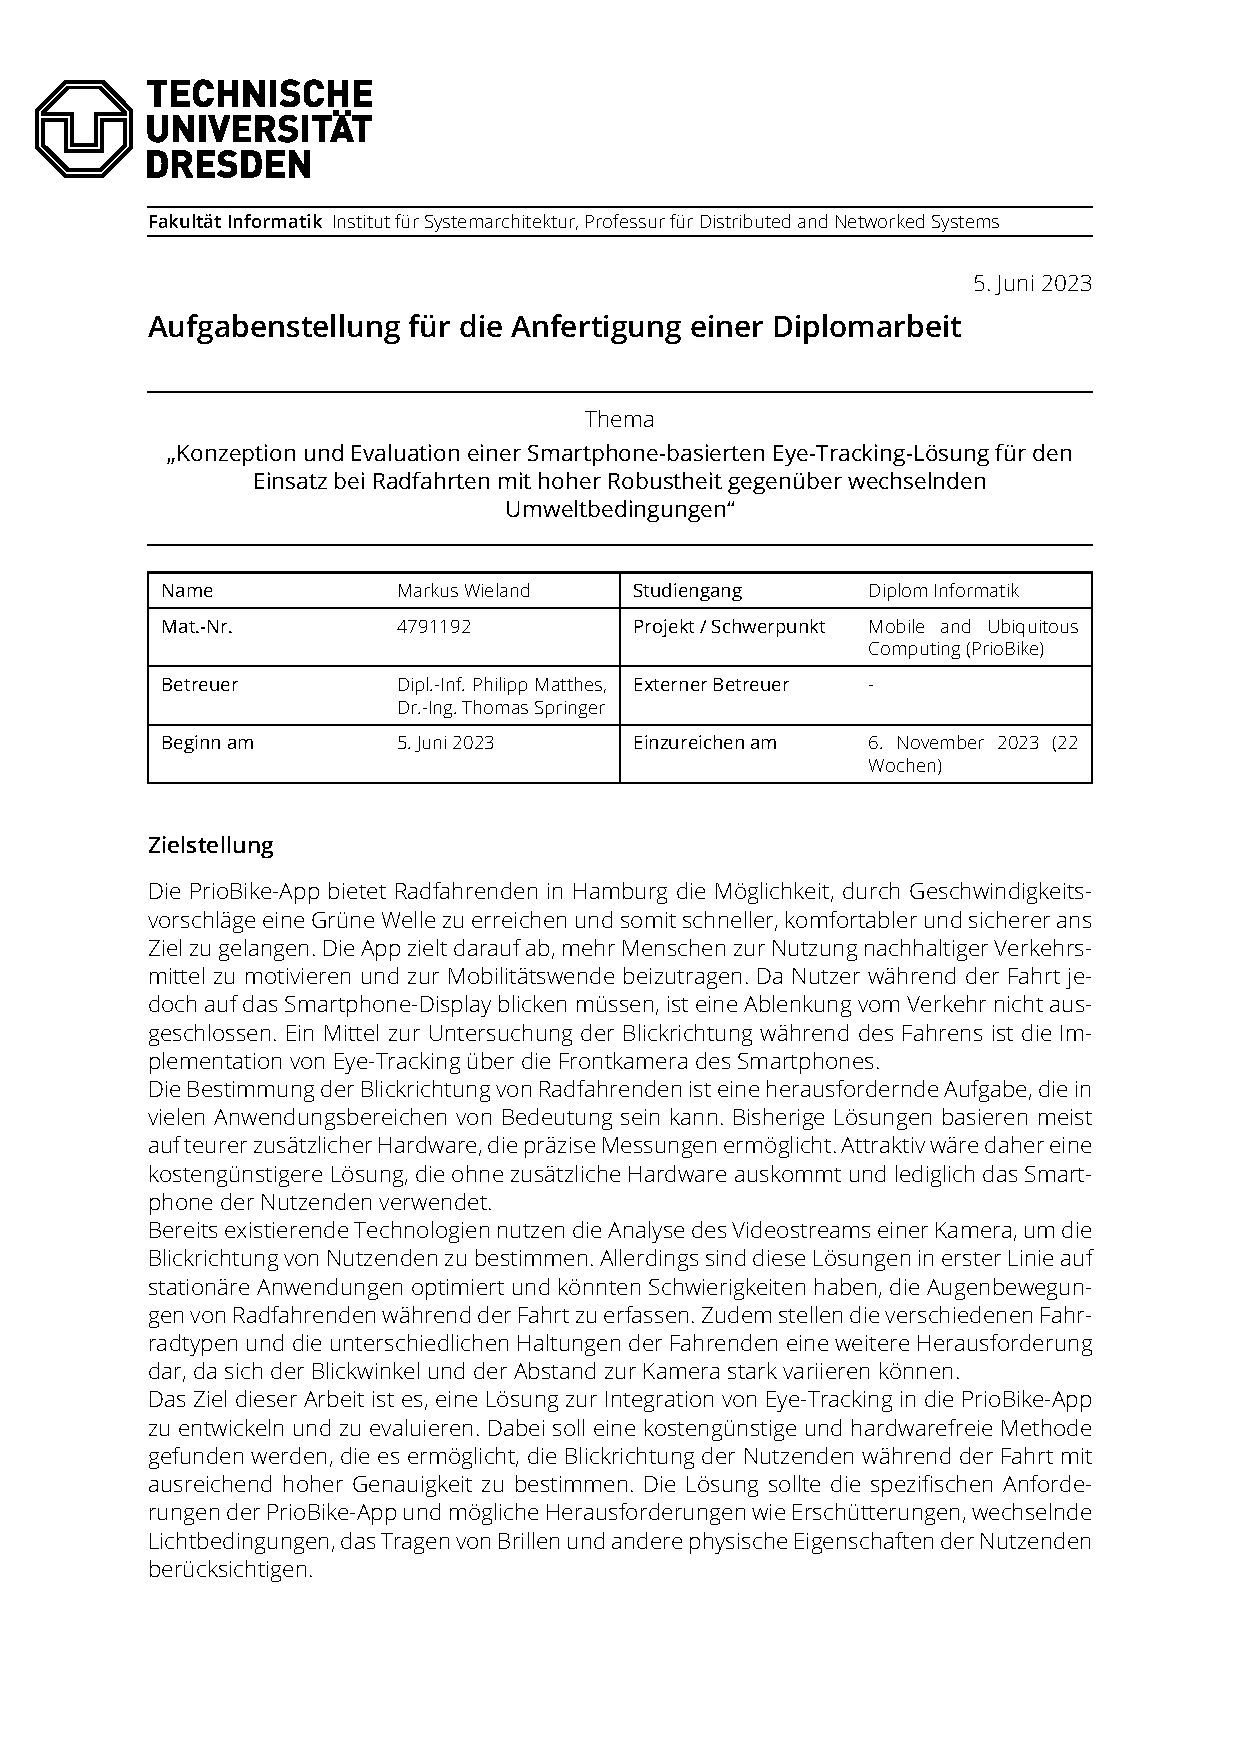
\includepdf[pages=-]{task/task.pdf}
  \newpage

  % for the order of the following sections please refer to
  % the recommendations for thesis structuring
  \confirmation

  \tableofcontents

  \listoffigures
  \addcontentsline{toc}{chapter}{\listfigurename}

  \listoftables
  \addcontentsline{toc}{chapter}{\listtablename}

  % this is where your thesis lives

  \chapter{Einleitung}\label{sec:introduction}\pagenumbering{arabic}

\section{Motivation}\label{sec:introduction:motivation}

Die Klimakrise ist zweifellos eine der größten Herausforderungen unserer Zeit. Ein Hauptgrund dafür ist der städtische Verkehr, der oft von vollen Straßen, Stau und Lärm geprägt ist, was zu hohen $\text{CO}_\text{2}$- und Feinstaubemissionen führt. Eine mögliche Lösung, um den Verkehr in Städten zu entlasten und umweltfreundlicher zu gestalten, ist die Förderung des Fahrradfahrens. Aus diesem Grund hat die Stadt Hamburg das \textit{PrioBike} Projekt\footnote{\url{https://www.hamburg.de/bvm/priobike/} (Abgerufen am 08.11.2023)} ins Leben gerufen. Es zielt darauf ab, das Fahrradfahren in der Stadt attraktiver und revolutionärer zu gestalten. 

Neben speziellen Fahrradstreifen und Anpassungen der Lichtsignalanlagen in der Stadt wird eine App für Radfahrende von der Technischen Universität Dresden entwickelt\footnote{\url{https://tu-dresden.de/bu/verkehr/vis/vpa/forschung/Individualverkehr/priobike} (Abgerufen am 08.11.2023)}. Diese App ermöglicht eine für Fahrräder optimierte Navigation durch die Stadt. Dabei werden während der Fahrt Ampeldaten genutzt, die von der Stadt Hamburg bereitgestellt werden, um den Nutzenden der App eine Geschwindigkeitsempfehlung zu geben, mit der diese die nächste Lichtsignalanlage bei Grün erreichen können, ohne an roten Ampeln warten zu müssen. Weitere Daten wie das Wetter oder die Oberflächenbeschaffenheit der Straßen sollen genutzt werden, um in der App nicht nur die schnellste oder kürzeste Route bereitzustellen, sondern auch die sicherste und attraktivste Route. 

Um die App während der Fahrt zu verwenden, kann man das Smartphone mit einer Halterung am Lenker des Fahrrads befestigen. Die Verwendung des Smartphones während der Fahrt birgt jedoch Risiken, da die Radfahrenden leicht abgelenkt werden können, wodurch eine gefährliche Situationen im Straßenverkehr entstehen kann. 

Um Ablenkungen durch die PrioBike-App zu vermeiden, sollen unübersichtliche oder ablenkende Ansichten in der App identifiziert und überarbeitet werden. Gleichzeitig wird an Features geforscht, die dazu beitragen sollen, dass Personen während der Fahrt seltener auf ihr Smartphone schauen müssen. Ein Beispiel für ein solches Feature wird in der Arbeit von Pickhardt \cite{diplom:paul:pickhardt} präsentiert. Diese Arbeit beschäftigt sich mit der Entwicklung von multimodalen Interaktionsmethoden für die Geschwindigkeitsempfehlung der PrioBike-App durch vibrotaktile und auditive Signale.

Um herauszufinden, ob ein solche Funktion dazu beiträgt, dass Radfahrende weniger auf ihr Smartphone schauen, bzw. um ablenkende Ansichten in der App zu identifzieren, muss ermittelt werden, zu welchen Zeitpunkten und über welchen Zeitraum die Personen auf ihr Smartphone schauen. Da eine Befragung der Personen häufig durch Bias beeinträgt ist, sollte die Erfassung der Daten durch eine Messung geschehen, um eine quantitative Auswertung zu ermöglichen. Daher soll im Rahmen dieser Arbeit untersucht werden, wie geeignet die Smartphones der Nutzenden sind, um eine solche Messung der Blickrichtung durchzuführen.

\section{Problem- und Zielstellung}\label{sec:introduction:goal}

Die Bestimmung der Blickrichtung von Menschen ist eine anspruchsvolle Aufgabe, welche in vielen Anwendungsbereichen relevant sein kann. Infolgedessen wurde bereits umfangreiche Forschung betrieben, um die Blickrichtungsverfolgung von Menschen zu optimieren. So wurden zahlreiche unterschiedliche Technologien entwickelt, die teilweise sehr präzise Messungen der Blickrichtung erlauben. Diese Technologien basieren jedoch meist auf teurer, zusätzlicher Hardware und erfordern eine Kalibrierung, um optimale Ergebnisse zu erzielen.

Für den Anwendungsfall der PrioBike-App ist jedoch eine kostengünstige Lösung notwendig, da während einer Testphase der App die Daten von vielen verschiedenen Teilnehmenden gesammelt werden sollen. Da die Teilnehmenden durch die Nutzung der PrioBike-App ihr Smartphone bereits am Fahrradlenker befestigt haben, wäre eine Lösung ideal, die ohne zusätzliche Hardware und Kalibrierung auskommt und nur mit der Innenkamera der Smartphones funktioniert.

Es existieren bereits Lösungen, die anhand der Analyse des Videostreams einer Kamera die Blickrichtung von Menschen bestimmen können. Diese sind nicht so präzise, erlauben aber trotzdem eine gute Annäherung, was im Fall der PrioBike-App ausreichend ist. Solche Technologien werden auch bereits in Anwendungen für mobile Geräte verwendet. Diese sind jedoch hauptsächlich für ruhende Menschen optimiert, welche frontal zur Kamera positioniert sind. In der Priobike-App ergeben sich jedoch Probleme aufgrund der unterschiedlichen Fahrradkonstruktionen und der damit verbundenen Körperhaltung. So können der Abstand zur Kamera und die Ausrichtung des Kopfes relativ zur Kamera stark variieren. Dies kann dazu führen, dass die Smartphone-Kamera einen schwierigen Blickwinkel auf die Gesichter der Personen hat, wodurch die Augen möglicherweise nur teilweise oder gar nicht zu sehen sind.

Die Nutzenden der PrioBike-App verwenden die App während der Fahrt mit dem Fahrrad. Der Videostream der Frontkamera kann daher durch verschiedene Umgebungsbedingungen beeinträchtigt werden. Vibrationen, die durch den Fahrstil der Nutzenden oder durch die Fahrbahnoberfläche verursacht werden, können das aufgenommene Bild verzerren, was bei bestehenden Lösungen zu Problemen bei der Erfassung der Augenbewegungen der Personen führen kann. 

Ein weiteres Problem ist die Umgebung der Nutzenden während der Fahrt. Durch die Montage des Smartphones am Lenker, filmt die Frontkamera größtenteils den Himmel. Dadurch ist mit wechselnden und vor allem schwierigen Lichtverhältnissen zu rechnen. Auch andere Umwelteinflüsse wie das Wetter können die Messgenauigkeit einschränken.

Eine weitere Herausforderung stellt die visuelle Vielfalt der verschiedenen Beteiligten an der Studie dar. Es ist anzunehmen, dass ein nicht unwesentlicher Teil der Nutzenden auf das Tragen eine Brille angewiesen ist. Das Glas der Brille kann Licht reflektieren und so die Augen unkenntlich machen. Je nach Form der Brille könnte diese auch Teile der Augen verdecken. Bei sonnigem Wetter könnten die Teilnehmenden eine Sonnenbrille tragen, was das Erkennen der Augen ebenfalls sehr erschweren könnte. Dazu kommen weitere körperliche Eigenschaften, wie unterschiedliche Haare, welche bei manchen Nutzenden Teile des Gesichts verdecken.
 
Im Rahmen dieser Arbeit soll die Eignung bestehender Ansätze für den speziellen Anwendungsfall der Messung während der Fahrradfahrt untersucht werden, um ein für die PrioBike-App optimiertes Verfahren zu entwickeln. Dieses Verfahren soll robust gegenüber den oben genannten Problemen sein, die durch die Umgebung, die individuelle Vielfalt der Menschen und den Blickwinkel der Kamera auf die Menschen während der Fahrt entstehen können. Um dieses Ziel zu erreichen, sollen folgende Forschungsfragen beantwortet werden:

\begin{researchquestion}\label{rq:best_possibility}
Was ist die beste Möglichkeit, nur mittels der Frontkamera eines mobilen Geräts die Blickrichtung der Nutzenden während der Fahrt zu verfolgen?
\end{researchquestion}

\begin{researchquestion}\label{rq:precision}
Wie präzise lässt sich mit der Frontkamera eines Smartphones, welches am
Lenker eines Fahrrads befestigt ist, bestimmen, zu welchen Zeitpunkten eine Person während der Fahrt auf das Smartphone sieht?
\end{researchquestion}

\begin{researchquestion}\label{rq:technical_problems}
Welche technischen Hürden sind zu überwinden, um eine Blickrichtungserkennung mittels
Smartphones auf einem Fahrrad zu entwickeln?
\end{researchquestion}

\begin{researchquestion}\label{rq:qc}
Wie kann die Qualität der aufgezeichneten Daten maximiert und Fehler minimiert werden?
\end{researchquestion}

\begin{researchquestion}\label{rq:umwelt}
Wie gut können die genannten Umwelteinflüsse (Licht, Erschütterungen) kompensiert werden?
\end{researchquestion}

\begin{researchquestion}\label{rq:verdeckt}
Wie gut lässt sich die Messung durchführen, wenn Teile des Gesichts der Person verdeckt sind?
\end{researchquestion}

\begin{researchquestion}\label{rq:kalibrierung}
Welche Kalibrierungen müssen zwingend vorgenommen werden, damit das Eye-Tracking funktioniert?
\end{researchquestion}

\section{Struktur der Arbeit}\label{sec:introduction:structure}

In diesem Kapitel wird der Aufbau der Arbeit vorgestellt. Zunächst werden in Kapitel \ref{sec:basics} Grundlagen vermittelt, die für das allgemeine Verständnis der Arbeit relevant sind. Dabei wird zunächst die Funktionsweise des menschlichen Auges erläutert. Anschließend wird ein Überblick über verschiedene Möglichkeiten gegeben, die Blickrichtung eines Menschen zu bestimmen. Außerdem werden Metriken vorgestellt, die in dieser Arbeit für die Evaluation verwendet werden.

In Kapitel \ref{sec:related} werden verwandte Arbeiten diskutiert. Insbesondere wird in diesem Kapitel die Bachelorarbeit von Henseler \cite{bachelor:henseler:gaze-ebikes} vorgestellt. In dieser beschäftigte sich Henseler bereits mit der Entwicklung eines Konzepts zur Bestimmung der Blickrichtung von Radfahrenden mittels der Innenkamera eines Smartphones. Es wird diskutiert, ob dieser Ansatz auch im Rahmen der PrioBike-App genutzt werden kann. Des Weiteren wird der aktuelle Stand der Forschung zu Methoden der Blickrichtungsbestimmung vorgestellt. Dabei wird auf verschiedene Ansätze eingegangen, die sich entweder mit der Blickrichtungsbestimmung mit Smartphones oder mit der Blickrichtungsbestimmung aus dem Videofeed einer Kamera beschäftigen. Abschließend wird ein Überblick über Arbeiten gegeben, die sich mit der Erkennung von Gesichtern in einem Bild beschäftigen, da dies während der Recherche als wichtiger Teilschritt identifiziert wurde.

Anhand der Erkenntnisse aus den verwandten Arbeiten wurden verschiedene Ansätze identifiziert, die danach in Kapitel \ref{sec:concept} auf ihre Eignung für den Einsatz in der PrioBike-App untersucht werden. Darauf aufbauend werden zwei unterschiedliche Konzepte zur Bestimmung der Blickrichtung von Radfahrenden entwickelt. 

In Kapitel \ref{sec:implementation} wird die Implementierung der beiden Konzepte vorgestellt. Zunächst wird ein allgemeiner Überblick über die Funktionsweise der Implementierung gegeben. Anschließend wird beschrieben, wie die einzelnen Schritte der beiden Konzepte umgesetzt wurden.

Anschließend wird die Evaluation der Konzepte in Kapitel \ref{sec:evaluation} vorgestellt. Dazu wird die Planung und Vorbereitung der Evaluation beschrieben und die Ergebnisse der Evaluation vorgestellt und diskutiert.

Abschließend werden in Kapitel \ref{sec:fazit} anhand der Ergebnisse die Forschungsfragen 
beantwortet. Darüber hinaus werden verschiedene Schwächen und Stärken dieser Arbeit diskutiert und weitere Forschungsrichtungen aufgezeigt, die auf dieser Arbeit aufbauen können.





  \chapter{Grundlagen}\label{sec:basics}

In diesem Kapitel werden Themen vorgestellt, die für das generelle Verständnis der Arbeit benötigt werden. Dafür wird zunächst die grobe Funktionsweise des menschlichen Auges beschrieben. Weiter wird vorgestellt, welche verschiedenen Methoden es gibt, um die Blickrichtung eines Menschen zu bestimmen. Anschließend werden Convolutional Neural Networks vorgestellt. Am Ende werden Metriken präsentiert, die für die Evaluation dieser Arbeit verwendet werden.

\section{Funktionsweise des menschlichen Auges}\label{sec:basics:eye}

Um unsere Umwelt optisch wahrnehmen zu können, wandelt das menschliche Auge Licht in elektrische Signale um. Das Licht fällt dabei zunächst durch die Pupille des Auges, wird im Auge gebrochen und auf die Netzhaut \cite[S.~12]{book:eyes} projiziert. Auf der Netzhaut befinden sich lichtempfindliche Zellen, die das einfallende Licht in elektrische Signale umwandeln können. Man unterscheidet zwischen Zapfen und Stäbchen. Die Zapfen sind die Zellen, mit denen der Mensch Farben wahrnehmen kann. Die Stäbchen hingegen können auch schwache Lichtreize wahrnehmen und ermöglichen so das Sehen bei schlechten Lichtverhältnissen. Über den Sehnerv werden die Signale an den visuellen Cortex weitergeleitet. So nennt man den Teil des menschlichen Gehirns, der die elektrischen Signale zu einem Bild zusammensetzt \cite[S.~13]{book:eyes}\cite{paper:cnn}. 

Auf der Netzhaut gibt es einen Bereich, in dem besonders viele Zapfen vorhanden sind. Diesen Bereich nennt man den gelben Fleck \cite[S.~13]{book:eyes}. Um etwas scharf sehen zu können, muss das Auge so bewegt werden, dass das Licht direkt auf diesen Bereich fällt. Die Linie zwischen dem Punkt, den das Auge dabei fixiert, und dem gelben Fleck wird Sichtlinie oder visuelle Achse genannt und gibt die Blickrichtung eines Menschen an \cite{paper:basic:eye:tracking}. Daneben gibt es noch die Blicklinie oder optische Achse, die die Verbindung der Pupille mit dem Zentrum des Augapfels beschreibt \cite{paper:basic:eye:tracking}.

Bei der dreidimensionalen Betrachtung der Blickrichtung einer Person spielt neben den Augenbewegungen auch die Kopfdrehung eine Rolle. Diese können als Drehung um drei verschiedene Achsen beschrieben werden. Die erste Achse ist die Querachse, auch horizontale Achse genannt. Der Winkel, um den der Kopf oder das Auge um diese Achse gedreht wird, wird als \textit{Pitch} bezeichnet. Dieser beschreibt die Rotation nach oben und unten. Dann gibt es die Vertikalachse. Sie beschreibt die Drehung nach links und rechts. Die Drehung um diese Achse wird mit dem \textit{Yaw}-Winkel angegeben. Die dritte Achse ist die Längsachse, die das Kippen des Kopfes nach links und rechts beschreibt. Der Winkel, um den der Kopf dabei gekippt wird, wird als \textit{Roll}-Winkel bezeichnet. Die Achsen sind in der Abbildung \ref{fig:basics:axis} dargestellt.

\begin{figure}[]
    \centering
    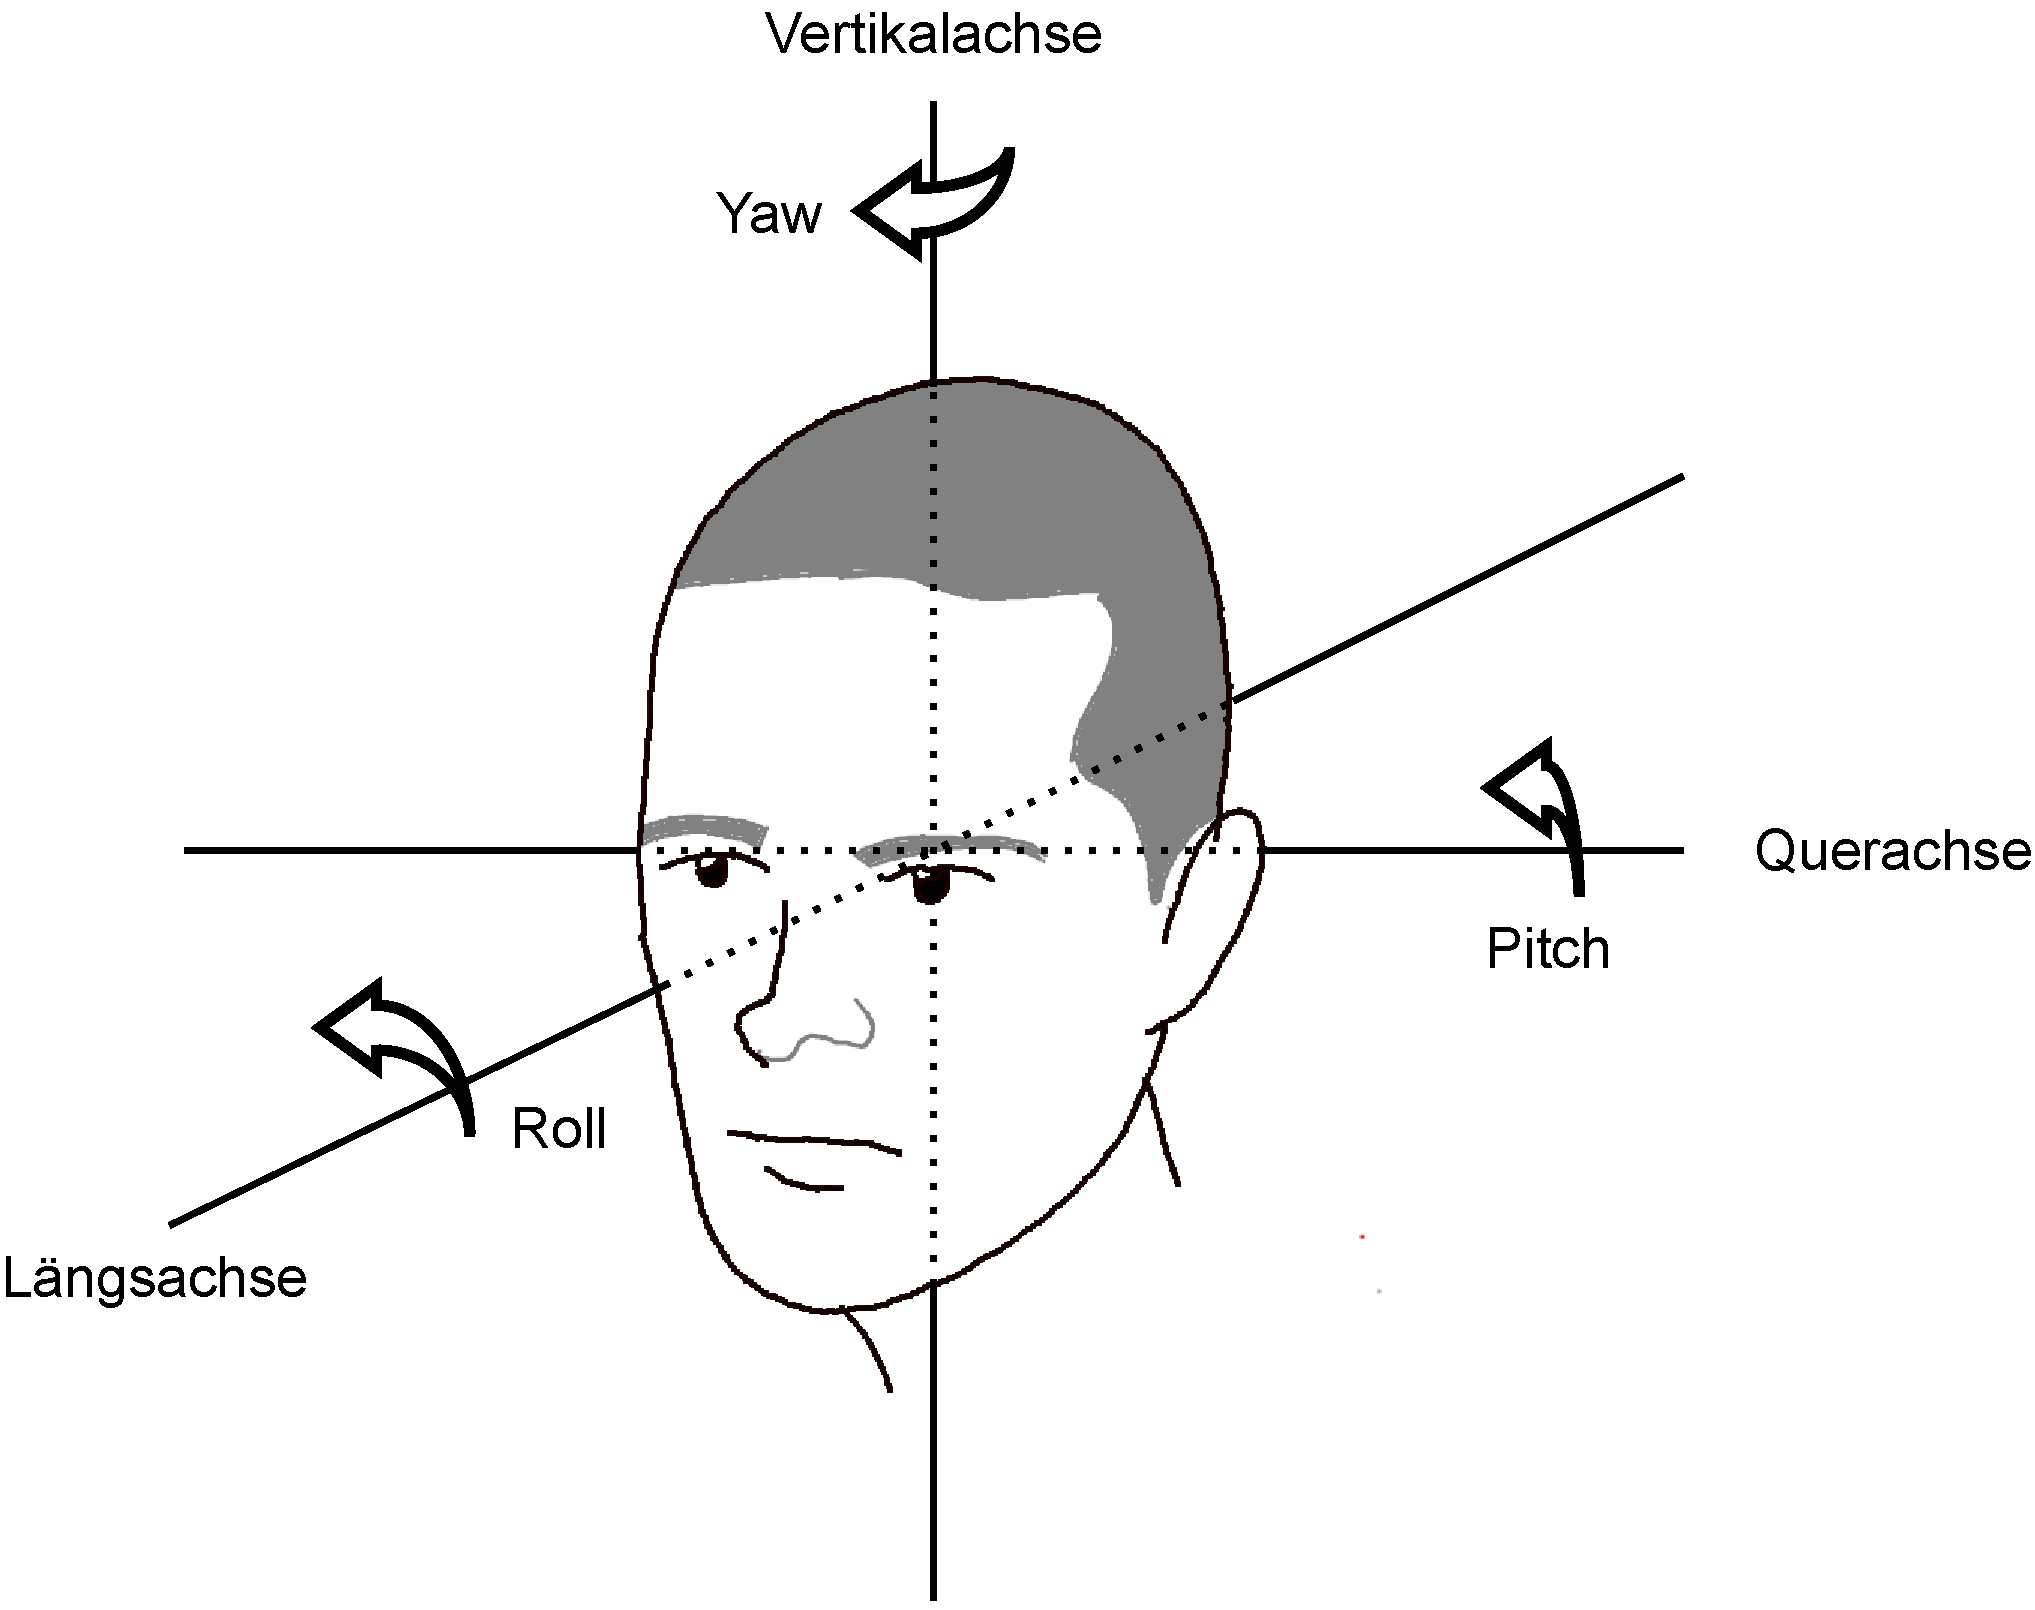
\includegraphics[width=0.8\linewidth]{basics/head.pdf}
    \caption{Darstellung der Quer-, Längs- und Vertikalachse des Kopfes eines Menschen. Quelle: Abbildung nach \cite{paper:eye-coordinates}}
    \label{fig:basics:axis}
\end{figure}

\section{Methoden zur Bestimmung der Blickrichtung}

In diesem Abschnitt werden verschiedene Methoden vorgestellt, die es ermöglichen die Blickrichtung einer Person zu bestimmen.

Das erste Verfahren ist die \textit{Elektrookulographie}. Bei diesem Verfahren werden die Augenbewegungen gemessen, um die Blickrichtung eines Menschen zu bestimmen. Zur Messung der Augenbewegung werden Elektroden links und rechts bzw. oberhalb und unterhalb der Augen angebracht. Aus der zwischen diesen Elektroden abgeleiteten Spannung können Rückschlüsse auf die Augenbewegung gezogen werden. Diese Methode ist daher nur für spezielle Anwendungsfälle geeignet \cite{paper:basics:survey}\cite[S.~70]{book:eyes}. 

Weiter lässt sich die Blickrichtung mittels \textit{3D Eye Model Recovery-Based} Methoden \cite{paper:basics:survey} bestimmen. Bei diesem Verfahren wird mithilfe von zusätzlicher Hardware wie Infrarotkameras ein dreidimensionales geometrisches Modell des Auges rekonstruiert. Für die Konstruktion dieses Modells werden jedoch personenspezifische Werte des Auges benötigt, die durch eine Kalibrierung ermittelt werden müssen. Ein solches Verfahren liefert genaue Vorhersagen über die Blickrichtung, kann aber immer nur für eine Person verwendet werden. Für jede weitere Person muss die Kalibrierung erneut durchgeführt werden. Außerdem wird, wie bereits erwähnt, zusätzliche Hardware benötigt, was die Einsatzmöglichkeiten dieses Verfahrens ebenfalls limitiert \cite{paper:basics:survey}. 

Bei \textit{2D Feature Regression-Based Methoden} \cite{paper:basics:survey} werden ebenfalls mit zusätzlicher Hardware geometrische Eigenschaften des Auges erfasst. Diese Eigenschaften können z.B. das Zentrum der Pupille oder die Reflektion von Lichtquellen auf der Hornhaut des Auges sein. Anhand der erkannten Merkmale, kann dann mit einer Regressionsfunktion bestimmt werden, wohin eine Person sieht \cite{paper:basics:survey}.

Es gibt Verfahren, die ohne zusätzliche Hardware und nur mit einer Kamera auskommen. Dabei handelt es sich um die \textit{Deep Learning Appearance-Based} \cite{paper:basics:survey} Verfahren. Sie nutzen das Bild einer Person, um Informationen über die Blickrichtung der Person zu extrahieren und darauf aufbauend die Blickrichtung vorherzusagen. Diese Verfahren benötigen jedoch eine große Menge an Trainingsdaten, um eine zuverlässige Blickrichtungsbestimmung zu ermöglichen. Dabei ist die Wahl des Datensatzes für den jeweiligen Anwendungsfall entscheidend. In der Regel sind die Ergebnisse eines solchen Ansatzes nicht so genau wie Verfahren, die auf zusätzlicher Hardware basieren \cite{paper:basics:survey}. Sie benötigen jedoch keine Kalibrierung, sind kostengünstiger und können ohne Einschränkungen eingesetzt werden. Ein weiterer Vorteil ist, dass sich die Personen bei solchen Verfahren uneingeschränkt bewegen können.

\section{Convolutional Neural Networks}

Eine Architektur von Neuronalen Netzen, die für Deep Learning Methoden verwendet werden kann, sind \textit{Convolutional Neural Networks}. \cite{diplom:matthes, paper:cnn}. Diese eignen sich sehr gut zur Erkennung von Mustern in Bildern \cite{diplom:matthes, paper:eth-xgaze, paper:mpiigaze, paper:rt_gene, paper:gaze360}. Als Eingabe dient ein Raster von Pixelwerten der zu verarbeitenden Bilder. Der generelle Aufbau von Convolutional Neural Networks besteht im Wesentlichen aus mehreren \textit{Convolution}-Schichten, denen jeweils eine \textit{Pooling}-Schicht \cite{paper:cnn} folgt. In den Convolution-Schichten werden Filter verwendet, um Muster in den Bilddaten zu erkennen. Ein solcher Filter ist eine kleine Matrix, die über das Raster der Pixelwerte verschoben wird und eine Punktprodukt-Operation mit den Pixelwerten durchführt. So können in diesen Schichten Muster wie Kanten und andere visuelle Informationen extrahiert werden \cite{diplom:matthes, paper:cnn}. In der anschließenden Pooling-Schicht wird die Dimensionalität der Daten reduziert, wobei die wichtigen Informationen erhalten bleiben \cite{paper:cnn}. In einer abschließenden \textit{Fully Connected}-Schicht werden die extrahierten Merkmale der vorhergehenden Schichten verwendet, um eine Klassifikation vorzunehmen, wie z.B. die ermittelte Blickrichtung der abgebildeten Person.

\section{Metriken für binäre Entscheidungen}

In diesem Abschnitt werden Metriken vorgestellt, die für die Evaluation dieser Arbeit verwendet werden. Die grundlegende Entscheidung, die in dieser Arbeit getroffen werden muss, ist, zu welchen Zeitpunkten die Radfahrenden auf ihr Smartphone schauen. Dabei handelt es sich um eine binäre Entscheidung, d.h. die Person schaut auf das Smartphone oder die Person schaut nicht auf das Smartphone. Zur Bewertung dieser Entscheidung wird eine Ground Truth benötigt, die den tatsächlichen Zustand zu einem bestimmten Zeitpunkt repräsentiert. Die Ground Truth kann in positive und negative Instanzen unterteilt werden. Die positiven Instanzen sind in diesem Beispiel die Zeitpunkte, zu denen die Person auf das Smartphone schaut. Die negativen Instanzen sind die Zeitpunkte, zu denen die Person nicht auf das Smartphone schaut. Anhand der Ground Truth kann jede Vorhersage, einer von vier Klassen zugeordnet werden \cite{diplom:matthes}.

Zunächst gibt es die \textit{True Positives} ($TP$). Eine Entscheidung gehört zu dieser Klasse, wenn richtig vorhergesagt wurde, dass der positive Fall eingetreten ist. In diesem Fall würde das bedeuten, dass richtig erkannt wurde, dass die Person auf das Smartphone schaut. Analog dazu gibt es die \textit{True Negatives} ($TN$). Diese geben in diesem Beispiel an, dass richtig vorhergesagt wurde, dass die Person nicht auf das Smartphone schaut. Für falsche Entscheidungen gibt es die \textit{False Positives} ($FP$) und die \textit{False Negatives} ($FN$). Zu den \textit{False Positives} gehören die Entscheidungen, bei denen erkannt wurde, dass die Person auf das Smartphone schaut, die Person aber zu diesem Zeitpunkt nicht auf das Smartphone geschaut hat. Die \textit{False Negatives} hingegen beschreiben, dass nicht erkannt werden konnte, dass die Person zu einem bestimmten Zeitpunkt auf das Smartphone geschaut hat.

Aus dieser vier Klassen lassen sich die Metriken \textit{Recall} und \textit{Precision} bestimmen. Der \textit{Recall} ist das Verhältnis der richtig vorhergesagten positiven Instanzen ($TP$) zur Gesamtzahl der positiven Instanzen in der Ground Truth. Die Gesamtzahl kann als Summe der \textit{True Positives} und der \textit{False Negatives} definiert werden \cite{diplom:matthes}. Der Recall kann somit wie folgt berechnet werden:

\[
\text{Recall} = \frac{TP}{TP + FN}
\]

Die Metrik \textit{Precision} beschreibt, wie viele positive Vorhersagen richtig waren \cite{diplom:matthes}. Dabei wird das Verhältnis der \textit{True Positives} zur Summe der \textit{True Positives} und \textit{False Positives} berechnet:

\[
\text{Precision} = \frac{TP}{TP + FP} \\
\]

Aus diesen beiden Metriken lässt sich die Metrik \textit{F1-Score} bestimmen. Diese Metrik ermöglicht es, \textit{Precision} und \textit{Recall} in einer gemeinsamen Metrik \cite{diplom:matthes} abzubilden. Der \textit{F1-Score} beschreibt dabei das harmonische Mittel zwischen den beiden Metriken.

\[
\text{F1-Score} = 2 \cdot \left( \frac{\text{Precision} \cdot \text{Recall}}{\text{Precision} + \text{Recall}} \right)
\]

Der kleinstmögliche Wert des \textit{F1-Scores} ist 0. Tritt dieser Fall ein, bedeutet das, dass entweder \textit{Precision} oder \textit{Recall} gleich 0 sind. Der bestmögliche Wert für den \textit{F1-Score} ist 1, was bedeutet, dass bei der Bestimmung keine falsche Vorhersage getroffen wurde.

\section{Zusammenfassung}

In diesem Kapitel wurden die wichtigsten Grundlagen für das Verständnis der Arbeit erläutert. Zunächst wurde die Funktionsweise des Auges dargestellt. Darauf aufbauend konnte erklärt werden, dass die Blickrichtung eines Menschen durch die Linie zwischen Pupille, gelbem Fleck und dem betrachteten Objekt definiert werden kann. Weiterhin wurde gezeigt, wie die Bewegung der Augen bzw. des Kopfes eines Menschen durch Drehung um drei verschiedene Achsen mit den Winkeln \textit{Pitch}, \textit{Yaw} und \textit{Roll} angegeben werden kann.  

Anschließend wurden verschiedene Methoden zur Bestimmung der Blickrichtung vorgestellt.  Diese lassen sich im Wesentlichen in zwei Kategorien einteilen: Methoden, die auf zusätzlicher Hardware basieren und Methoden, die mittels Deep Learning auf Basis eines Kamerabildes arbeiten. Für diese Deep Learning Appearance-Based Methoden eignen sich insbesondere Convolutional Neural Networks, deren Funktionsweise ebenfalls vorgestellt wurde. 

Abschließend wurden die Metriken \textit{Recall}, \textit{Precision} und \textit{F1-Score} vorgestellt, die zur Evaluation dieser Arbeit verwendet werden. 



  
  \chapter{Verwandte Arbeiten}\label{sec:related}

In diesem Kapitel wird ein Überblick über verwandte Arbeiten gegeben. Dazu wird zunächst die Arbeit von Henseler \cite{bachelor:henseler:gaze-ebikes} vorgestellt, die sich speziell mit der Blickrichtungsbestimmung von Radfahrenden beschäftigt. Anschließend werden Arbeiten vorgestellt, die sich mit Deep Learning Appearance-Based Methoden zur Bestimmung der Blickrichtung aus dem Bild einer Person beschäftigen. Während der Recherche wurde festgestellt, dass die Gesichtserkennung bei diesen Methoden eine wichtige Rolle spielt. Daher werden im Anschluss Arbeiten vorgestellt, die sich mit der Erkennung von Gesichtern in einem Bild beschäftigen.

\section{Bachelor-Arbeit Matthias Henseler}\label{sec:related:henseler}

Henseler beschäftigt sich in seiner Arbeit \cite{bachelor:henseler:gaze-ebikes} mit der Entwicklung einer Blickrichtungserkennung für Personen auf einem E-Bike mittels des Videostreams der Innenkamera von einem Smartphone. Ziel der Arbeit war es eine Methode zu entwickeln, mit der sich bestimmen lässt, wohin eine dargestellte Person während der Fahrradfahrt sieht. Dabei soll die Blickrichtung in eine der folgenden Kategorien eingeteilt werden:

\begin{itemize}
\item Geradeaus
\item Rechts, stark rechts
\item Links, stark links
\item Lenker rechts, Lenker Mitte (Smartphone), Lenker links
\end{itemize}

Das Smartphone wird dabei in einer speziell für diese Arbeit angefertigten Halterung befestigt. Sie ist nicht wie üblich am Lenker des Fahrrads montiert sondern am Fahrradrahmen. Diese Halterung wurde entwickelt, da eine Halterung am Lenker beim Fahren in einer Kurve zusammen mit dem Lenker einknickt und dadurch der Blickwinkel der Kamera auf den Radfahrenden verändert wird. Dies würde den Ansatz von Henseler beeinträchtigen, wie später in diesem Kapitel erläutert wird. Die Halterung wurde speziell für ein Smartphone entwickelt, mit welchem anschließend alle Tests durchgeführt wurden. Durch diese Limitation ist der Ansatz nicht sehr flexibel, da diese spezielle Halterung und das entsprechende Smartphone benötigt werden, wenn eine andere Person diesen Ansatz nutzen möchte. 

Zur Bestimmung der Blickrichtung müssen mit dem Ansatz von Henseler verschiedene Merkmale im Gesicht der abgebildeten Person identifiziert werden. Das erste Merkmal ist eine Bounding Box, die das gesamte Gesicht der Person umfasst. Für die Gesichtserkennung wird ein Binärbild basierend auf den Pixeln erstellt, die innerhalb eines vordefinierten Farbbereichs liegen, welcher die Hautfarbe darstellen soll. Ein solches Binärbild zeigt einen weißen Pixel, wenn der entsprechende Pixel des Originalbilds in dem vordefinierten Farbbereich liegt. Liegt der Farbwert außerhalb des Bereichs, wird ein schwarzer Pixel zu dem Binärbild hinzugefügt. Henseler beschreibt, dass der Erfolg der Gesichtserkennung durch den vordefinierten Farbbereich sehr von den aktuellen Beleuchtungsbedingungen abhängt. Eine weitere Limitation ist, dass es schwer ist mit diesem Ansatz die Diversität der menschlichen Hautfarbe abzubilden. Im nächsten Schritt werden Lücken im Binärbild geschlossen, die beispielsweise durch den Kinnriemen des Helms oder eine Sonnenbrille entstehen. Anschließend wird innerhalb des Binärbildes nach Gruppen von zusammenhängenden Pixeln gesucht, welche eine vordefinierte Größe aufweisen. Wenn eine solche Gruppe gefunden wird, wird angenommen, dass es sich dabei um das Gesicht handelt. Für diese Gruppe wird dann eine Bounding Box berechnet, die es ermöglicht, das Gesicht im Originalbild auszuschneiden. Wenn keine passende Gruppe gefunden wird, bedeutet das, dass kein Gesicht in diesem Bild erkannt werden konnte. Wenn kein Gesicht erkannt wird, kann keine Aussage über die Blickrichtung getroffen werden, da alle weiteren Merkmale, die zur Bestimmung der Blickrichtung benötigt werden, auf der Erkennung des Gesicht beruhen. 

Das nächste Merkmal, das erkannt werden soll, ist die Stirn des Radfahrenden. Da dies allerdings schwierig ist, wenn die Person einen Helm und eine Sonnenbrille trägt, wurde stattdessen ein gelber Klebestreifen an der unteren Kante des Helms des Radfahrenden angebracht. Anstelle der Stirn muss also der Klebestreifen im Bild erkannt werden. Dafür wird nach Pixeln mit einem Farbwert innerhalb eines vordefinierten Farbbereichs gesucht, um erneut ein Binärbild zu berechnen. Anschließend werden erneut Gruppen von zusammenhängenden Pixeln in dem Binärbild gesucht. Da zu erwarten ist, dass sich der Klebestreifen im oberen Bereich des erkannten Gesichts befindet, können diese Gruppen anhand ihrer Größe und Position gefiltert werden.

Zum Schluss müssen die Nase und der Mund der Person erkannt werden. Für die Erkennung der Nase wird das Originalbild zuerst anhand unterschiedlicher Farbbereiche in mehrere Binärbilder aufgeteilt. Anschließend wird in jedem dieser entstandenen Binärbilder nach zusammenhängenden Pixelgruppen gesucht, um potentielle Nasenlöcher zu erkennen. Dafür werden zunächst Gruppen außerhalb der Bounding Box des Gesichts verworfen. Dann werden die erkannten Gruppen nach Größe und Form gefiltert. Zum Schluss wird bei den verbleibenden Gruppen nach solchen gesucht, die sich ungefähr auf einer horizontalen Linie befinden und einen Abstand von 5 bis 19 Pixeln voneinander haben. Falls damit immer noch keine Nase erkannt werden kann, wird die Position der Nase aus dem vorherigen Frame genutzt. 
Um den Mund zu erkennen, wird das Bild zunächst in Graustufen umgewandelt. Die Erkennung des Mundes erfolgt dann mittels eines vortrainierten Haarcascade-Classifiers. Henseler beschreibt, dass dadurch für fast jedes Bild mehrere Münder erkannt werden. Es wird sich für den erkannten Mund entschieden, dessen Zentrum sich unter der erkannten Nase befindet. Wenn kein Mund erkannt wurde, wird angenommen, dass sich dieser 20 Pixel unterhalb der Nase befindet.

Das Erkennen von Gesichtsmerkmalen erfolgt direkt auf dem Smartphone. Das Konzept wurde als Android-App umgesetzt und erreicht eine Leistung von 7 bis 15 Bildern pro Sekunde. Zur Realisierung des beschriebenen Prozesses wird die Android-Bibliothek von \textit{OpenCV}\footnote{\url{https://opencv.org/releases/} (Zugriff am 05.11.2023)} genutzt, welche Algorithmen für Computer-Vision-Aufgaben sowie Bildverarbeitung bereitstellt. 

Mithilfe der erkannten Merkmale der Person wird dann die Blickrichtung in eine der acht oben genannten Kategorien eingeordnet. Die Bestimmung wird dabei in zwei Teile geteilt. Zunächst wird die Rotation entlang der Querachse bestimmt. Dabei wird eine binäre Entscheidung getroffen, ob die Person nach oben auf den Straßenverkehr oder nach unten auf den Lenker des Fahrrads sieht. Des Weiteren muss die Rotation entlang der Vertikalachse des Kopfes bestimmt werden. Dabei wird zwischen den Kategorien \textit{stark links}, \textit{links}, \textit{geradeaus}, \textit{rechts} und \textit{stark rechts} unterschieden. Die Klassifizierung nach \textit{stark rechts} und \textit{stark links} erfolgt nur dann, wenn die Person auf den Straßenverkehr und nicht auf den Lenker sieht.

Für die Berechnung wird als erstes eine Strecke zwischen dem Mittelpunkt des erkannten Mundes und der erkannten Nasen berechnet. Dann wird der Mittelpunkt dieser Strecke bestimmt. Dieser Punkt wird im Folgenden als $P_{\text{MN}}$ bezeichnet. Für die binäre Entscheidung, ob die dargestellte Person auf den Lenker sieht oder nicht, wird die Distanz $d_{\text{KMN}}$ zwischen dem Mittelpunkt des erkannten Klebestreifens und dem Punkt $P_{\text{MN}}$ berechnet. Der Kamerawinkel des Smartphones sorgt dafür, dass $d_{\text{KMN}}$ bei Bildern, bei denen die Person auf das Smartphone sieht, größer ist als bei Bildern, bei denen die Person auf den Straßenverkehr schaut. Dieser Abstand ist allerdings von Person zu Person unterschiedlich und hängt auch sehr von der Sitzposition der Person ab. Aus diesem Grund kann kein vordefinierter Grenzwert festgelegt werden. Dieser muss für jede Person einzeln bestimmt werden. Diese Kalibrierung findet zu Beginn der Fahrt statt. Wenn die gemessene Distanz $d_{\text{KMN}}$ größer als der bestimmte Grenzwert ist, schaut die Person auf den Lenker. Andernfalls schaut die Person nach oben und betrachtet den Straßenverkehr.

Für die Bestimmung der Rotation entlang der Querachse des Kopfes wird die ermittelte Bounding Box des Kopfes in fünf verschiedene Zonen unterteilt, wie in der Abbildung \ref{fig:related:henseler:box} zu sehen ist. Die Höhe der Zonen entspricht der Höhe der Bounding Box. Die Breite der mittleren Zone entspricht 40\% der Breite der Bounding Box des Kopfes. Die Breite der anderen Zonen beträgt jeweils 15\% der Breite der Bounding Box. Nun wird überprüft, in welcher der Zonen sich der Punkt $P_{\text{MN}}$ befindet. Befindet sich der Punkt $P_{\text{MN}}$ in einer der äußeren Zone, so schaut die Person nach \textit{stark links} bzw. \textit{stark rechts}. Befindet sich der Punkt in der mittleren Zone, schaut die Person \textit{geradeaus}. Befindet sich der Punkt in einer der verbleibenden Zonen, schaut die Person nach \textit{links} oder \textit{rechts}. 
Um Fehldetektionen zu vermeiden, wird eine ermittelte Blickrichtung nur dann als legitim angesehen, wenn zwei aufeinander folgende Bilder gleich klassifiziert wurden. Henseler beschreibt dies als eine weitere Einschränkung seines Ansatzes, da so schnelle Kopfbewegungen unter Umständen nicht erkannt werden können und bei Übergängen zwischen zwei Blickrichtungen immer mindestens ein Bild keine legitime Blickrichtungsbestimmung hat.

\begin{figure}
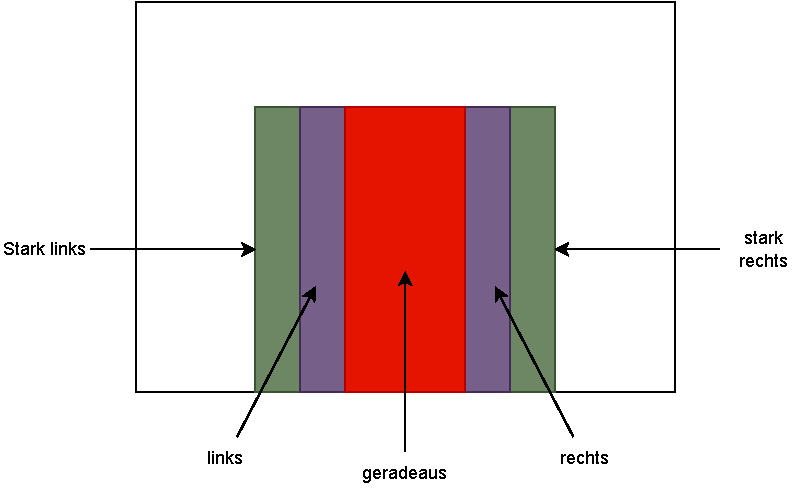
\includegraphics[width=0.7\linewidth]{concept/henseler-aufbau-kopf.pdf}
\caption{Einteilung der Bounding Box des Kopfes (grün dargestellt) in Zonen. Die blaue Zone hat eine Größe von 70\% der grünen Zonen. Die rote Zone hat eine Größe von 40\% der grünen Zone. Quelle: Abbildung nach \cite{bachelor:henseler:gaze-ebikes}.}
\label{fig:related:henseler:box}
\end{figure}

Für die Bewertung dieses Ansatzes wurden insgesamt 160 Minuten Videomaterial aufgezeichnet, das drei verschiedene Personen zeigt. Es wird darauf hingewiesen, dass in den meisten Videos die abgebildete Person eine Sonnenbrille trägt. Alle Videos wurden bei sonnigem oder leicht bewölktem Wetter aufgenommen. Andere Tageszeiten oder Wetterbedingungen wurden nicht berücksichtigt, da der von Henseler beschriebene Ansatz zur Gesichtserkennung nur bei einem gut beleuchteten Gesicht funktioniert. Bei stark bewölktem Himmel stellt die automatische Helligkeitsanpassung der Kamera des Smartphones laut Henseler ein Problem dar, da dadurch das Gesicht nicht ausreichend hell genug ist, um es zu erkennen. 

Aus den aufgezeichneten Videos wurden in regelmäßigen Abständen 1.516 Einzelbilder ausgewählt und separat gespeichert. Anschließend hat Henseler diese manuell in eine der acht oben genannten Kategorien eingeordnet, um eine Ground Truth zu erstellen. Ein Problem, das während der Erstellung der Ground Truth aufgetreten ist, war die Einordnung von Randfällen, bei denen es beispielsweise schwierig war zu entscheiden, ob die abgebildete Person nach links oder stark nach links schaut. Eine interessante Tendenz, die an den Daten der Ground Truth ersichtlich wird, ist, dass nur in jeweils zwei Fällen die Personen links oder rechts auf den Lenker geschaut haben, während insgesamt 49 Mal auf die Mitte des Lenkers (Smartphone) gesehen wurde. Dies weist darauf hin, dass Radfahrende vor allem auf ihr Smartphone schauen, wenn sie ihren Blick vom Straßenverkehr abwenden.

Nach der Erstellung der Ground Truth wurden die Bilder von dem implementierten Ansatz von Henseler verarbeitet. Dabei wurden die erkannten Gesichtsmerkmale in jedem Bild markiert und separat gespeichert. Diese Bilder wurden anschließend ebenfalls manuell ausgewertet. Dabei wurde für jedes Merkmal die binäre Entscheidung getroffen, ob das Merkmal richtig erkannt wurde oder nicht. Diese Entscheidung basierte auf der Einschätzung von Henseler.  

Das Ergebnis war, dass nur in 964 Bildern ein Gesicht erkannt werden konnte. Da die weitere Erkennung der Blickrichtung auf dem erkannten Gesicht basiert, kann somit bei den restlichen 552 Bilder keine Aussage darüber getroffen werden, wohin die dargestellte Person schaut, was eine große Schwäche des Ansatzes von Henseler ist.

Die weitere Auswertung wurde daher nur für die Bilder mit erkanntem Gesicht fortgesetzt. Von den 964 Bildern mit erkanntem Gesicht wurden bei 805 Bildern die Blickrichtung entsprechend der Ground Truth richtig klassifiziert. Die meisten Fehler sind auf eine falsche Erkennung der Nase oder des Mundes zurückzuführen. Die größten Ungenauigkeiten traten bei der Erkennung der Kategorie \textit{Lenker mitte} (Smartphone) auf. Von insgesamt 49 Bildern konnte die Kategorie nur bei 31 Bildern richtig zugeordnet werden.

Zusammenfassend kann gesagt werden, dass es Henseler gelungen ist, eine Blickrichtungserkennung von Radfahrenden zu realisieren. Mit dieser lassen sich gute Ergebnisse erzielen, wenn in einem Bild ein Gesicht erkannt werden kann. Eine besondere Stärke ist, dass teilweise verdeckte Gesichter, wie zum Beispiel durch Sonnenbrillen, erkannt werden können. Für einen Einsatz im Rahmen der PrioBike-App ist dieser Ansatz jedoch nicht geeignet. Dies liegt zum einen an der zusätzlichen Hardware in Form der Halterung des Smartphones am Fahrradrahmen und dem notwendigen gelben Klebestreifen am Fahrradhelm, ohne die der Ansatz nicht funktioniert. Eine weitere Schwäche ist, dass keine Aussage über die Blickrichtung getroffen werden kann, wenn kein Gesicht erkannt wurde, was bei Henseler bei gut einem Drittel aller Bilder der Fall ist. Außerdem ist für das PrioBike-Projekt vor allem wichtig zu erkennen, wann die Person auf das Smartphone schaut, was bei Henselers Ansatz die schlechtesten Ergebnisse lieferte. Die generelle Idee, die Blickrichtung anhand der Kopfrotation zu bestimmen, wird jedoch als vielversprechend angesehen und soll in dieser Arbeit aufgegriffen werden.

\section{Blickrichtungsbestimmung}\label{sec:related:gaze}

Im Folgenden werden Arbeiten vorgestellt, die sich mit verschiedenen Methoden zur Blickrichtungsbestimmung beschäftigen. Dabei werden sowohl Arbeiten speziell für Smartphones als auch allgemeine Methoden zur Blickrichtungsbestimmung betrachtet.

\subsection{MobiGaze}\label{sec:related:gaze:model:mobigaze}

Eine frühe Arbeit, die sich mit der Bestimmung der Blickrichtung auf Smartphone-Displays beschäftigt, ist die Arbeit von Nagamatsu et al. \cite{paper:mobigaze}. Da die einhändige Bedienung von Smartphones umständlich ist, wollten die Autoren einen Ansatz entwickeln, der die Blickrichtung einer Person nutzt, um eine Interaktion mit dem Smartphone zu ermöglichen. Zu diesem Zweck entwickelten Nagamatsu et al. \textit{MobiGaze}. Dabei handelt es sich um ein System, das aus zwei zusätzlichen Kameras und einer Infrarot-LED besteht, die am Smartphone angebracht werden. Mit diesen kann die dreidimensionale Blickrichtung des Menschen bestimmt werden. \textit{MobiGaze} ist so konzipiert, dass es dabei egal ist, wie die Person das Smartphone hält, solange die Augen von den Kameras erfasst werden können. Da die Rechenleistung von Smartphones damals noch nicht ausreichte, um die Berechnungen direkt auf dem Gerät durchzuführen, war bei diesem Ansatz zusätzlich ein Computer notwendig. Dieser hat die Berechnung der Blickrichtung durchgeführt und das Ergebnis an das Smartphone übermittelte.  

Mit dieser Interaktionsmethode stellen die Autoren einige mögliche Anwendungen vor, die darauf basieren, eine Auswahl anhand des Blicks zu treffen und diese in Kombination mit einem Druck auf das Smartphone zu bestätigen \cite{paper:mobigaze}. Damit zeigen die Autoren, dass eine dreidimensionale Blickrichtungsbestimmung für den Einsatz auf Smartphones möglich ist, auch wenn diese Methode auf zusätzlicher Hardware basiert, was sie für die Blickrichtungsbestimmung von Radfahrenden ungeeignet macht. 

\subsection{WebGazer}\label{sec:related:webgazer}\label{sec:related:gaze:appearance:webgazer}

Eine Arbeit, die sich damit beschäftigt, die Blickrichtungsbestimmung der Allgemeinheit zugänglich zu machen, ist die Arbeit von Papoutski et al. \cite{paper:webgazer}, in der sie \textit{WebGazer} vorstellen. Bei dieser Arbeit handelt es sich um eine JavaScript-Bibliothek, die in jede beliebige Webseite eingebunden werden kann. Mit \textit{WebGazer} können die Punkte auf dem Bildschirm ermittelt werden, die eine Person beim Betrachten einer Webseite ansieht. \textit{WebGazer} ist dabei nicht auf spezielle zusätzliche Hardware angewiesen, sondern ermöglicht die Blickrichtungsbestimmung mittels einer Webcam. 

Die Blickrichtungsbestimmung funktioniert dabei so, dass zunächst die Augen der Person im Bild der Webcam erkannt werden\footnote{In ihrer Arbeit verwenden Papoutsaki et al. drei verschiedene Methoden, um die Augen zu erkennen. Diese sind \textit{clmtrackr} \url{https://github.com/auduno/clmtrackr} (Abgerufen am 08.11.2023), \textit{js-objectdetect} \url{https://github.com/mtschirs/js-objectdetect} (Abgerufen am 08.11.2023), und \textit{tracking.js} \url{https://trackingjs.com/} (Abgerufen am 08.11.2023)}. Anhand der erkannten Augen kann die Blickrichtung anschließend mit zwei verschiedenen Methoden bestimmt werden. Bei dem ersten Ansatz wird die Position der Pupille des Auges erkannt, anhand derer die Bildschirmkoordinaten linear geschätzt werden. 

Für den zweiten Ansatz untersuchten Papoutski et al. den Zusammenhang zwischen den Blicken und den Interaktionen von Menschen mit einer Website. Zunächst wurden Mausklicks untersucht. Die Autoren stellten fest, dass Personen dorthin schauen, wohin sie klicken. Anschließend untersuchten sie die Mausbewegungen und stellten fest, dass diese den Blicken mit einer leichten Verzögerung folgen. Mit diesen Erkenntnissen und einem mehrdimensionalen Merkmalsvektor, den die Autoren aus dem Bild der Augen extrahierten, können so mittels einer Regressionsfunktion die Bildschirmkoordinaten bestimmt werden, auf die die Person schaut. 

Da die Implementierung von \textit{WebGazer} frei zugänglich ist und einfach in jede Webseite integriert werden kann, könnte diese Methode für die Bestimmung der Blickrichtung auf einem Smartphone implementiert werden. Damit bietet \textit{WebGazer} eine Möglichkeit, die Stellen des Displays zu identifizieren, auf die Radfahrende während der Fahrt schauen. Es ist jedoch unklar, ob mit dieser Methode unterschieden werden kann, ob eine Person auf das Display schaut oder nicht.

\subsection{Übersicht über Deep Learning Appearance-Based Methoden}\label{sec:related:gaze:appearance}

Die Bestimmung der Blickrichtung von Menschen mithilfe von Deep Learning Appearance-Based Methoden ist ein Thema, mit dem sich einige Forschungsarbeiten beschäftigen. Cheng et al. geben in ihrer Arbeit \cite{paper:basics:survey} einen Überblick über den aktuellen Stand der Forschung zu diesen Methoden.

Dafür präsentieren die Autoren zunächst die gängigen Schritten, die während der Umsetzung dieser Methode ausgeführt werden. Nach der Aufnahme eines Bildes einer Person mit einer Kamera ist es zunächst erforderlich, das Gesicht oder die Augen dieser Person innerhalb des Bildes zu erkennen. Dadurch kann das Bild auf den für die Betrachtung relevanten Bereich des Gesichts zugeschnitten werden, wodurch unwichtige Informationen aus dem Rest des Bildes eliminiert werden können.

Cheng et al. beschreiben darüber hinaus ein Verfahren, mit dem weitere Störfaktoren aus dem Bild entfernt werden können. Diese Störfaktoren entstehen vor allem dadurch, dass sich die Personen bei Appearance-Based Methoden frei bewegen können. Dadurch ist eine große Variation der Kopfdrehung möglich. Die Drehung des Kopfes um die Längsachse kann bei solchen Verfahren jedoch ignoriert werden, da sich die generelle Orientierung des Gesichts zur Kamera durch sie nicht ändert. Außerdem kann die Entfernung des Gesichts zur Kamera während der Aufnahme der Bilder variieren. Das oben genannte Verfahren von Cheng et al. vermeidet diese beiden Störfaktoren. Dazu wird zunächst ein Referenzpunkt im Gesicht der Person festgelegt. Anschließend wird die Kamera virtuell so verschoben, dass sie sich direkt über diesem Referenzpunkt befindet. Anschließend wird das Bild so gedreht, dass die Drehung des Kopfes um die Längsachse aufgehoben wird. Im letzten Schritt wird das Bild so skaliert, dass das Gesicht einen festen virtuellen Abstand zur Kamera hat \cite{paper:basics:survey}. Das Verfahren ist beispielhaft in der Abbildung \ref{fig:related:normalisierung} dargestellt.

\begin{figure}
    \centering
    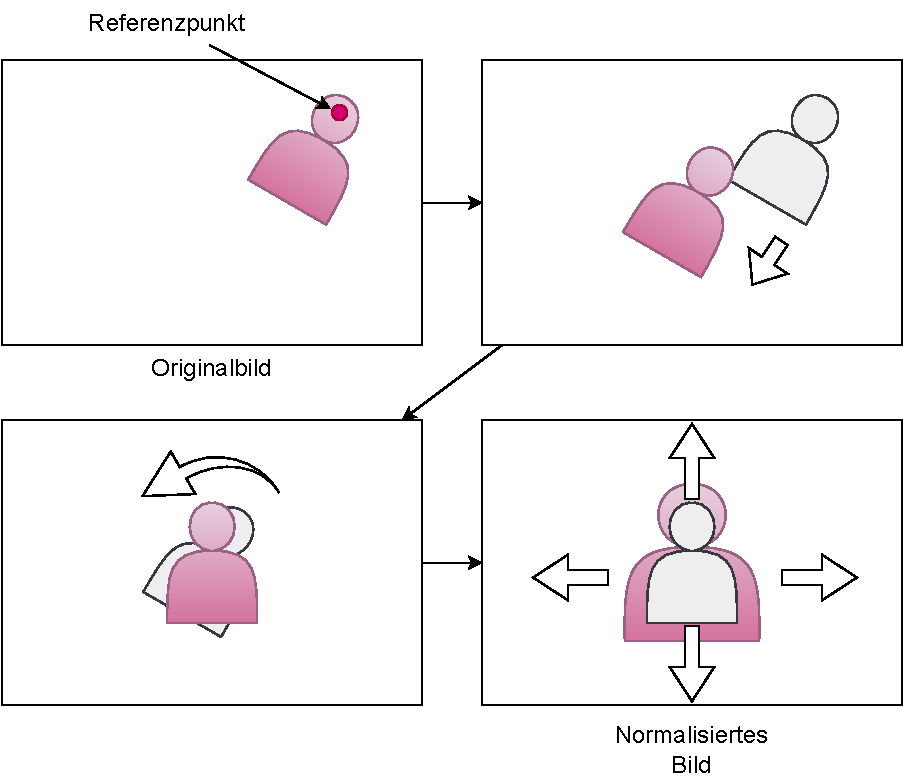
\includegraphics[width=0.8\linewidth]{related/normalisierung.pdf}
    \caption{Beispielhafte Darstellung der Normalisierung von Bildern. Quelle: Abbildung nach \cite{paper:basics:survey}}
    \label{fig:related:normalisierung}
\end{figure}

Das normalisierte Bild wird dann von einem neuronalen Netz verarbeitet, um auf die Blickrichtung der Person zu schließen. Für diese Aufgabe eignen sich besonders Convolutional Neural Networks \cite{paper:basics:survey, paper:cnn, diplom:matthes}. Eine wichtige Entscheidung, die dabei getroffen werden muss, ist die Wahl des Datensatzes, der als Grundlage für das Convolutional Neural Network verwendet wird. Cheng et al. geben in ihrer Arbeit \cite{paper:basics:survey} einen Überblick über verschiedene Datensätze. Je nach Anwendungsfall sind verschiedene Datensätze unterschiedlich gut geeignet. Eine Auswahl dieser Datensätze wird im weiteren Verlauf des Kapitels vorgestellt.

Die Vorhersage eines solchen Convolutional Neural Networks ist dann, je nach Wahl der Trainingsdaten, ein zweidimensionaler Punkt auf einem Bildschirm oder eine dreidimensionale Blickrichtung, die durch einen Pitch- und einen Yaw-Winkel angegeben wird \cite{paper:basics:survey}. Es ist zu beachten, dass sich die Vorhersage auf das normalisierte Gesicht bezieht, wenn die Bilder normalisiert wurden. Die entsprechenden Ergebnisse müssen daher umgerechnet werden, damit sie dem tatsächlich dargestellten Gesicht entsprechen.

Im Folgenden werden verschiedene Implementierungen von Convolutional Neural Networks sowie Datensätze vorgestellt, die für das Training verwendet werden können.

\subsubsection{Columbia}\label{sec:related:gaze:appearance:gaze-locking}

Smith et al. stellen in ihrer Arbeit \cite{paper:columbia} den \textit{Columbia} Datensatz vor. Dieser besteht aus 5.880 Bildern von 56 verschiedenen Personen, die unter Laborbedingungen aufgenommen wurden. Der Datensatz zeigt die Teilnehmenden in einer von fünf verschiedenen fixierten Kopfpositionen, bei denen der Kopf entlang der Vertikalachse gedreht wurde. Für jede der fünf Kopfpositionen wurden dann 21 verschiedene Ziele von den Teilnehmenden betrachtet. Somit können für jede Kopfposition 21 verschiedene Blickwinkel dargestellt werden. Durch die Fixierung des Kopfes, das Wissen, wohin die Person schaut und die Position der Kamera konnte für alle aufgenommenen Bilder ein dreidimensionaler Blickrichtungsvektor gespeichert werden, der als Ground Truth verwendet wird.

Ziel war es, mittels dieses Datensatzes einen Ansatz zu ermöglichen, den sie \textit{Gaze Locking} \cite{paper:columbia} nennen. Der Ansatz basiert auf der Tatsache, dass wir Menschen sehr gut erkennen können, ob eine Person uns ansieht oder nicht. Wir haben allerdings größere Schwierigkeiten, genau zu bestimmen, wohin eine Person schaut, wenn sie uns nicht ansieht. Daher wollten die Autoren das Problem der Blickrichtungsbestimmung vereinfachen, indem sie es zu einem binären Problem machen. Sie wollten anhand des Bildes einer Person entscheiden, ob diese Person in die Kamera schaut oder nicht.

Dafür trainierten sie anhand des Datensatzes ein Modell, das diese binäre Entscheidung treffen sollte. Das Modell erzielte sehr genaue Ergebnisse, auch bei großen Abständen zwischen Person und Kamera. Generell konnte die Arbeit zeigen, dass das Ziel der binären Entscheidung, ob eine Person in die Kamera schaut oder nicht, mithilfe des Modells umgesetzt werden konnte.
Der verwendete Datensatz von Smith et al. ist jedoch aufgrund der geringen Variation der Kopfpositionen nicht für die Bestimmung der Blickrichtung von Radfahrenden geeignet. Dies liegt vor allem daran, dass der Datensatz keine Variation der Kopfdrehung entlang der Querachse enthält. Aus Sicht der Innenkamera eines Smartphones ist jedoch vor allem die Kopfdrehung entlang der Querachse entscheidend dafür, ob Radfahrende auf das Smartphone schauen oder nicht.

\subsubsection{MPIIGaze \& MPIIFaceGaze}\label{sec:related:gaze:appearance:mpiigaze}

In einer Arbeit von Zhang et al. \cite{paper:mpiigaze, paper:mpiigaze-old} wird der \textit{MPIIGaze} Datensatz vorgestellt. Ziel der Arbeit war es, einen Datensatz zu entwickeln, der Menschen bei der Benutzung von Laptops in normalen Alltagssituationen zeigt und somit eine größere Variation von Kopfdrehungen, Hintergründen und Lichtverhältnissen darstellen kann. Dies wurde erreicht, indem 15 verschiedene Personen über einen längeren Zeitraum zu zufälligen Tageszeiten einen Punkt auf dem Bildschirm ihres Laptops fixierten. Dabei wurden Aufnahmen mit der Webcam des Laptops gemacht. Insgesamt wurden so 213.659 Bilder in verschiedenen Situationen aufgenommen. Für alle diese Bilder wurde ein dreidimensionaler Blickrichtungsvektor als Ground Truth bestimmt. 

Der Datensatz zeigt daher eine größere Variation der Kopfdrehung und der Lichtverhältnisse als der \textit{Columbia} \cite{paper:columbia} Datensatz. Aufgrund des notwendigen Blickkontakts der abgebildeten Person mit dem Bildschirm des Laptops ist der Datensatz jedoch in den abgebildeten Kopfdrehungen dennoch eingeschränkt. Der Blickwinkel einer Laptop-Webcam auf die Person vor ihr ist in den meisten Fällen nicht vergleichbar mit dem Blickwinkel eines Smartphones am Fahrradlenker auf Radfahrende. Es ist daher davon auszugehen, dass eine Verwendung des Datensatzes für den Anwendungsfall der PrioBike-App nicht geeignet ist.

Anhand ihres Datensatzes haben Zhang et al. \cite{paper:mpiigaze} anschließend ein Convolutional Neural Network entwickelt. Dazu wurden die Bilder des Datensatzes zunächst vorverarbeitet. Zuerst wurde das Gesicht innerhalb des Bildes identifiziert. Anschließend wurden verschiedene Gesichtspunkte in Form von zweidimensionalen Bildkoordinaten bestimmt \cite{paper:dlib}. Um den Einfluss der Gesichtsmerkmalserkennung auf die Ergebnisse des Convolutional Neural Networks zu untersuchen, wurden die korrekten Gesichtsmerkmale in einem Teil des Datensatzes bestimmt. Dazu wurden die Gesichtsmerkmale zunächst automatisch erkannt und anschließend von einem Menschen manuell korrigiert. Nach der Erkennung der Gesichtsmerkmale wurden diese verwendet, um die Augen der Person aus dem Bild zu extrahieren. Daraufhin wurde ein dreidimensionales Modell eines Kopfes erstellt, das auf dem Durchschnitt der im Datensatz gezeigten Personen basiert. Dieses Modell wurde verwendet, um die dreidimensionale Position der zweidimensionalen Bildkoordinaten \cite{paper:epnp} zu bestimmen. Mit diesem Verfahren konnten eine Rotationsmatrix und ein Translationsvektor bestimmt werden, die dann zur Normalisierung der Bilder mit der von Cheng et al. \cite{paper:basics:survey} vorgestellten Methode verwendet wurden. Aus dieser Normalisierung berechnen Zhang et al. einen Rotationsvektor $h$, der die Rotation des normalisierten Gesichts angibt. Da die Normalisierung die Rotation um die Längsachse eliminiert, kann der Vektor als zweidimensional betrachtet werden. Anhand der erkannten Gesichtsmerkmale werden dann die Augen aus dem Bild extrahiert. Mit $h$ und den Bildern der Augen wird dann das \cnn trainiert, um eine dreidimensionale Blickrichtung des normalisierten Kopfes zu bestimmen, die dann wieder in das ursprüngliche Koordinatensystem vor der Normalisierung umgerechnet werden kann.

In einer späteren Arbeit \cite{paper:mpiifacegaze} haben Zhang et al. untersucht, wie die Ergebnisse des Modells verbessert werden können, wenn nicht nur einzelne Augenbilder, sondern das gesamte Gesicht als Input verwendet wird. Diese Untersuchungen zeigten, dass die Verwendung des gesamten Gesichts die Qualität der Vorhersagen deutlich verbessern kann. Eine besonders wichtige Erkenntnis ihrer Arbeit war, dass das Modell vor allem bei schwierigen Lichtverhältnissen und extremen Kopfdrehungen deutlich bessere Ergebnisse erzielen konnte, was eine sehr wichtige Erkenntnis für die Anwendung einer solchen Methode im Rahmen der PrioBike-App ist.

\subsubsection{GazeCapture}\label{sec:related:gaze:appearance:gazecapture}

Krafka et al. stellen in ihrer Arbeit den Datensatz \textit{GazeCapture} vor \cite{paper:gazecapture}. Dieser Datensatz umfasst Bilder von 1.474 verschiedenen Personen und ist somit der Datensatz mit der größten Anzahl von verschiedenen Teilnehmenden. Er besteht aus 2.400.000 Bildern von Personen im täglichen Leben. Aufgenommen wurden die Bilder mit den Smartphones und Tablets der Personen. Der Datensatz spiegelt damit eine sehr große Diversität von verschiedenen Gesichtern, Accessoirs, Hintergründen und Beleuchtungebedingungen wieder. Dafür wurde eine Anwendung entwickelt, welche die Personen auf ihrem Gerät installieren konnten. Diese Anwendung zeigte den Teilnehmenden einen Punkt auf dem Bildschirm ihres Geräts, den sie fixieren sollten. Zusätzlich wurden die Teilnehmenden durch die Anwendung dazu motiviert, ihren Kopf zu bewegen und den Abstand zwischen dem Gerät und dem Kopf zu vergrößern. Für alle der dabei entstanden Bilder wurde die entsprechende Koordinate des Punktes auf dem Bildschirm, die Orientierung des Geräts sowie die Art des Geräts als Ground Truth gespeichert.

Aufbauend auf \textit{GazeCapture} entwickelten Krafka et al. \textit{iTracker} \cite{paper:gazecapture}. Dabei handelt es sich um einen \cnn, das aus den Bildern des Gesichts und der Augen einer Person und einer binären Maske, die die relative Position des Kopfes im Originalbild wiedergibt, eine zweidimensionale Koordinate für ein Gerät ermitteln kann. Dazu haben sie verschiedene Experimente durchgeführt und unter anderem \textit{iTracker*} entwickelt. Dieses Modell verwendet das Daten über die Orientierung und die Art des verwendeten Geräts, um die Ergebnisse zu maximieren. Mit ihrem Ansatz erzielten Krafka et al. einen durchschnittlichen Fehler von 1,04 cm bei Smartphones und 1,69 cm bei Tablets \cite{paper:gazecapture}.

Dieser Datensatz und das damit trainierte Modell beinhalten jedoch aufgrund der Art der Datenerhebung mit dem durchgehenden Blickkontakt der Person mit dem Display nur eine eingeschränkte Variation der Kopfdrehung, die nicht mit der Kopfdrehung von Radfahrenden vergleichbar ist, was diesen Datensatz für eine Verwendung in dieser Arbeit ungeeignet macht.

\subsubsection{TabletGaze}\label{sec:related:gaze:appearance:tabletgaze}

Ein weiterer Datensatz, der speziell mit Tablets aufgenommen wurde, wird von Huang et al. in ihrer Arbeit \cite{paper:tabletgaze} vorgestellt. Dabei handelt es sich um den \textit{Rice TabletGaze} Datensatz. Ziel des Datensatzes war es, eine unkalibrierte Bestimmung der Blickrichtung von Personen auf einem Tablet zu ermöglichen. Dazu wurde ein Datensatz erstellt, der auf 51 verschiedenen Personen basiert. Von diesen Personen wurden Videos mit der Innenkamera des Tablets aufgenommen, während sie das Tablet benutzten. Während der Aufnahme konnten sich die Teilnehmenden frei bewegen, es wurde lediglich eine von vier allgemeinen Körperhaltungen vorgegeben. Diese Körperhaltungen waren Sitzen, Liegen, Stehen und eine entspannte Haltung auf einem Sofa. Während der Nutzung des Tablets sollten die Probanden einen zufällig auf dem Bildschirm platzierten Punkt verfolgen. Mithilfe dieses Punktes wurde für jedes aufgenommene Bild die zweidimensionale Koordinate des Punktes als Ground Truth gespeichert.

Anschließend wurden die aufgenommenen Bilder gefiltert. So wurden Aufnahmen entfernt, die kurz nach dem Positionswechsel des Punktes gemacht wurden, um die Übergangsphase, in der sich die Person auf den neuen Punkt fixiert, zu eliminieren. Außerdem wurde versucht, die Augen der Person im Bild zu erkennen, um diese zu dem Datensatz hinzufügen zu können. Können keine Augen erkannt werden, werden auch diese Bilder aussortiert. Anschließend wird anhand der durchschnittlichen Pixelintensität im Bereich der Augen erkannt, ob die Augen geschlossen sind oder nicht. Wenn ein geschlossenes Auge erkannt wurde, wurde das entsprechende Bild sowie die Bilder direkt davor und danach entfernt. Auf diese Weise entstand ein Datensatz mit insgesamt 100.000 Einträgen.

In diesem Datensatz ist zwar auch eine Variation der Kopfdrehung enthalten, diese wird jedoch durch den ständigen Blickkontakt der Person mit dem Display des verwendeten Gerätes eingeschränkt, was diesen Datensatz für die Verwendung der Blickrichtungsbestimmung von Radfahrenden für diese Arbeit ungeeignet macht.

\subsubsection{RT-GENE}\label{sec:related:gaze:appearance:rt-gene}

Fischer et al. präsentieren in ihrer Arbeit den \textit{RT-GENE} Datensatz \cite{paper:rt_gene}. Dieser wurde dadurch motiviert, dass existierende Datensätze keine große Varianz bezüglich der Entfernung der Personen zur Kamera aufweisen. Der Datensatz besteht aus 15 verschiedenen Personen, von denen 122.531 Bilder aufgenommen wurden. Der Datensatz wurde unter Laborbedingungen aufgenommen. Dazu wurde eine Person in einem Raum platziert. Dieser Person wurde eine Halterung auf den Kopf gesetzt, in die ein Eye-Tracker integriert wurde. Die Aufgabe dieser Halterung ist es, die Blickrichtung zu messen. So kann der Kopf frei bewegt werden, ohne ein bestimmtes Ziel anvisieren zu müssen. Dieser Rahmen wurde so groß gestaltet, dass möglichst wenig von den Augen verdeckt wird. An dieser Halterung wurden vier Marker befestigt. Anhand dieser Marker konnte ein Motion-Capture-System die Kopfdrehung der Versuchspersonen ermitteln. Mit diesem Aufbau war es möglich, Bilder der Testperson aufzunehmen, bei denen die Testperson weiter von der Kamera entfernt stand und den Kopf frei bewegen konnte. Aus der gemessenen Blickrichtung des Eye-Trackers und der gemessenen Kopfhaltung des Motion-Capture-Systems konnte so für jedes Bild ein dreidimensionaler Blickrichtungsvektor ermittelt und gespeichert werden.

In diesen Bildern der Personen ist jedoch das Gestell mit dem integrierten Eye-Tracker zu erkennen, was in einem alltäglichen Anwendungsfall natürlich nicht der Fall wäre. Daher wird das Gestell mittels eines Generative Adversial Network (GAN) \cite{paper:gan} aus dem Originalbild entfernt. Der Datensatz wurde weiter gefiltert, indem Bilder entfernt wurden, bei denen die Kopfdrehung zu groß war, um beide Augen der Person zu erkennen. Bilder mit geschlossenen Augen wurden ebenfalls entfernt.

Der Datensatz zeigt ein breiteres Spektrum an Kopfdrehungen als die vorherigen Datensätze. Allerdings wurden die Bilder unter Laborbedingungen bei gleicher Beleuchtung aufgenommen, was für den Anwendungsfall der Blickrichtungsbestimmung beim Radfahren nicht ideal ist. 

Weiter stellen Fischer et al. einen Ansatz vor, diesen Datensatz zur Bestimmung der Blickrichtung von Personen zu verwenden \cite{paper:rt_gene}. Dazu werden zunächst markante Gesichtsmerkmale im Bild erkannt \cite{paper:mtcnn}. Anhand der erkannten Gesichtspunkte werden die Augen aus dem Originalbild ausgeschnitten. Anschließend wird das von Cheng et al. vorgestellte Verfahren zur Normalisierung der Bilder der Augen \cite{paper:basics:survey} angewendet. Diese werden separat in einen VGG-16 \cnn geladen. Damit ist es möglich, die dreidimensionale Blickrichtung einer Person durch den Pitch- und Yaw-Winkel zu bestimmen. Die Methode lieferte sehr gute Ergebnisse und konnte auch die maximale Performance anderer Datensätze, wie zum Beispiel \textit{MPIIGaze}, verbessern.

\subsubsection{Gaze360}\label{sec:related:gaze:appearance:gaze360}

Kellnhofer et al. stellen in ihrer Arbeit \cite{paper:gaze360} den Datensatz \textit{Gaze360} vor. Dabei handelt es sich um einen Datensatz, der sowohl Außen- als auch Innenaufnahmen enthält und eine große Variation von Kopfdrehungen zeigt. Der Datensatz besteht aus 238 verschiedenen Personen mit insgesamt 172.000 Aufnahmen. Zur Aufnahme der Bilder wurde eine 360°-Kamera verwendet. Um diese Kamera herum wurden verschiedene Personen in einem Abstand von zwei bis drei Metern aufgestellt. Eine weitere Person trägt ein Schild. Auf diesem Schild ist zum einen ein Code \cite{paper:april-tag} und zum anderen ein großer Punkt zu sehen. Auf diesen Punkt sollen die Teilnehmenden schauen, während die Person mit dem Schild um sie herumgeht. Der Aufnahmeprozess wurde dabei in zwei verschiedene Phasen unterteilt. In der ersten Phase war es den Teilnehmenden erlaubt, ihren Kopf zu bewegen, um so eine große Reichweite von verschiedenen Kopfdrehungen im Datensatz zu ermöglichen. In der zweiten Phase durften die Teilnehmenden ihren Kopf nicht bewegen und sollten den Punkt nur mittels der Augen verfolgen, um so auch eine große Reichweite von Blickwinkeln zu ermöglichen. Das Schild mit dem Punkt war dabei immer so ausgerichtet, dass der dargestellte Code auf dem Schild zur Kamera zeigt. Anhand des Codes wurde das Schild später in den Aufnahmen erkannt. So konnten Rückschlüsse auf die dreidimensionale Position des Punkt geschlossen werden. So konnte für jede Aufnahme ein dreidimensionaler Blickrichtungsvektor bestimmt werden. 
Durch die große Variation der Kopfdrehungen und dem Vorhandensein von Außenaufnahmen könnte dieser Datensatz gut geeignet sein, um eine Blickrichtungsbestimmung von Radfahrenden zu ermöglichen.

Darüber hinaus stellen Kellnhofer et al. in ihrer Arbeit  \cite{paper:gaze360} ein Modell zur Blickrichtungsbestimmung vor. Dieses basiert auf der Tatsache, dass die Bestimmung der Blickrichtung ein kontinuierlicher Prozess ist und daher die Blickrichtungen aufeinanderfolgender Bilder voneinander abhängig sind. Dafür verwenden wird die Autoren ein \cnn, bei dem als Eingabe sieben aufeinanderfolgende Bilder mit Gesichtern einer Person verwendet werden. Diese werden dann in bidirektionale Long Short-Term Memory Capsules (LSTM) \cite{paper:lstm} gegeben. Mittels einer Fully Connceted-Schicht wird dann die Blickrichtung vorhergesagt. Das Modell kann somit für die Vorhersage des aktuellen Bildes auch die Vorhersagen der drei vorhergehenden und der drei nachfolgenden Bilder zur Blickrichtungsbestimmung verwenden.

\subsubsection{L2CS-net}\label{sec:related:gaze:appearance:l2cs}

Abdelrahman et al. stellen in ihrer Arbeit \cite{paper:l2csnet} ein robustes \cnn zur Bestimmung der Blickrichtung in freien Umgebungen vor. Dazu verwenden sie die Datensätze \textit{MPIIGaze} und \textit{Gaze360}. Die Bilder der Datensätze werden zunächst mit dem von Cheng et al. \cite{paper:basics:survey} präsentierten Verfahren zur Normalisierung der Bilder verarbeitet. Für die Blickrichtungsbestimmung, verwenden die Autoren ein ResNet-50 \cnn. Das besondere an ihrem Ansatz ist, dass der Pitch- und der Yaw-Winkel, die die dreidimensionale Blickrichtung angeben, jeweils separat von einem Fully Connected Layer vorhergesagt werden. Mit diesem Ansatz konnten sie im Vergleich zu anderen Arbeiten in beiden Datensätzen den geringsten Blickrichtungsfehler erzielen. Ihre Implementierung des Verfahrens ist öffentlich zugänglich\footnote{\url{https://github.com/Ahmednull/L2CS-Net} (Abgerufen am 09.11.2023)}.


\subsubsection{ETH-XGaze}\label{sec:related:eth-xgaze}\label{sec:related:gaze:appearance:eth-xgaze}

In der Arbeit von Zhang et al. \cite{paper:eth-xgaze} wird der Datensatz \textit{ETH-XGaze} vorgestellt. Ziel der Arbeit war es, einen robusten Datensatz für die Bestimmung der Blickrichtung bei einer großen Variation von Kopfposen zu erstellen, da vorherige Arbeiten wie zum Beispiel \textit{MPIIGaze} \cite{paper:mpiigaze} oder \textit{RT-Gene} \cite{paper:rt_gene} sehr limitiert sind, was die Reichweite der Kopfrotation betrifft.

Der Datensatz von Zhang et al. umfasst 1.083.492 Bilder mit den dazugehörigen dreidimensionalen Blickrichtungen von insgesamt 110 Teilnehmenden im Alter von 19 bis 41 Jahren. Die Teilnehmenden stammen aus diversen Ethnien. 47 der Teilnehmenden sind weiblich, 63 sind männlich. Für die Erstellung des Datensatzes wurden die Teilnehmenden in einem Abstand von etwa einem Meter vor einen Bildschirm mit einer Größe von 120 $\times$ 100 cm platziert. Dabei wurden die Teilnehmenden von insgesamt vier Lichtquellen beleuchtet, welche links und rechts neben dem Bildschirm platziert wurden. Mit diesen Lichtquellen lassen sich durch das Ein- und Ausschalten einzelner Lichtquellen 16 verschiedene Beleuchtungsbedingungen simulieren. Um die Kopfrotation der Teilnehmenden während der Aufnahme zu messen, wurde der Kopf der Probanden fixiert. Die Teilnehmenden wurden dazu angehalten, ihren Kopf während des Experiments nicht zu bewegen. Um dennoch eine große Variation von Kopfposen zu ermöglichen, wurden die Teilnehmenden von 18 verschiedenen Kameras aufgenommen, welche alle einen anderen Blickwinkel auf die Probanden zeigen. Diese Kameras nehmen Bilder mit einer Auflösung von 6000 $\times$ 4000 Pixeln auf. 

Der Datensatz von Zhang et al. enthält im Vergleich zu den bisherigen Datensätzen die größte Vielfalt an Kopfrotationen und Blickwinkeln. Außerdem variieren die Einträge des Datensatzes stark in der Beleuchtung. Aufgrund der zu erwartenden Vielfalt an Kopfrotationen der Radfahrenden sowie der vielen unterschiedlichen Lichtbedingungen während der Fahrt ist dieser Datensatz vielversprechend für den Einsatz innerhalb der PrioBike-App.

Anhand des Datensatzes haben Zhang et al. anschließend ein \cnn mit einer Standard ResNet-50 Architektur trainiert. Für das Trainieren des Modells werden die Bilder vorab bearbeitet. Die Autoren beschreiben, dass dafür zunächst das Gesicht und anschließend die Gesichtsmerkmale innerhalb des Bildes erkannt werden. Um die dreidimensionale Kopfrotation der Person zu bestimmen, werden die erkannten zweidimensionalen Gesichtspunkte auf ein dreidimensionales Gesichtsmodell übertragen \cite{paper:eth-xgaze-3d-pose}. Mithilfe der dabei bestimmten Kopfrotation werden die Bilder anschließend mit der von Cheng et al. beschriebenen Methode \cite{paper:basics:survey} normalisiert.

Die Leistung des trainierten Modells wurden mit Modellen basierend auf Datensätze von anderen Arbeiten verglichen. Die Ergebnisse haben gezeigt, dass Zhang et al. mit ihrem Ansatz den geringsten Blickrichtungsfehler sowohl bei niedrigen als auch hohen Kopf- und Blickwinkeln erzielen konnten, was ebenfalls vielversprechend für den Einsatz der Arbeit im Rahmen des PrioBike-Projekts ist. 

\subsubsection{Zusammenfassung}


Cheng et al. stellen in ihrer Arbeit die allgemeine Vorgehensweise zur Bestimmung der Blickrichtung mit Deep Learning Appearance-Based Methoden vor. Darüber hinaus geben sie einen Überblick über verschiedene Implementierungen und Datensätze, die dafür verwendet werden können. Eine Übersicht über diese Datensätze ist in Tabelle \ref{tab:related:overview:gaze:angles} und Tabelle \ref{tab:related:overview:gaze:content} \cite{paper:eth-xgaze, paper:gaze360} dargestellt.

\begin{table}
\begin{tabular}{l c c c }
\toprule
                                        & \makecell{\textbf{Anzahl}\\\textbf{Personen}} & \makecell{\textbf{Variation}\\\textbf{Kopfdrehung}} & \makecell{\textbf{Variation}\\\textbf{Blickwinkel}} \\
\midrule
Columbia \cite{paper:columbia}          & 56    & 0\degree, $\pm$30\degree    & $\pm$15\degree, $\pm$10\degree  \\
MPIIGaze \cite{paper:mpiigaze}          & 15    & $\pm$15\degree, 30\degree   & $\pm$20\degree, $\pm$20\degree  \\ 
GazeCapture \cite{paper:gazecapture}    & 1.474 & $\pm$30\degree, 40\degree     & $\pm$20\degree, $\pm$20\degree  \\
RT-GENE \cite{paper:rt_gene}            & 15    & $\pm$40\degree, $\pm$40\degree  & $\pm$40\degree, -40\degree    \\
Gaze360 \cite{paper:gaze360}            & 238   & $\pm$90\degree, unknown       & $\pm$140\degree, -50\degree   \\
ETH-XGaze \cite{paper:eth-xgaze}        & 110   & $\pm$80\degree, $\pm$80\degree  & $\pm$120\degree, $\pm$70\degree \\
\bottomrule
\end{tabular}
\caption{Überblick über die vorgestellten Datensätze. Die Tabelle beinhaltet die Anzahl der Personen in einem Datensatz sowie die dargestellte maximale Kopfdrehung (Yaw, Pitch) und den maximalen Blickwinkel (Yaw, Pitch). Die angebenen Reichweiten der Kopfdrehung und Blickwinkel entstammen der Arbeit von Zhang et al. \cite{paper:eth-xgaze}. Der \textit{TabletGaze} Datensatz wird in der Arbeit von Zhang et al. \cite{paper:eth-xgaze} nicht aufgeführt.}
\label{tab:related:overview:gaze:angles}
\end{table}

\begin{table}
\begin{tabular}{l c c c c c}
\toprule
                                        & \textbf{\#Daten} & \textbf{Auflösung} & \textbf{Outdoor} & \textbf{Gaze} & \textbf{Image}  \\
\midrule

Columbia \cite{paper:columbia}          &  5.880     & $5.184 \times 3.456$ & \xmark & \textcolor{blue}{3D} & Gesicht\\
MPIIGaze \cite{paper:mpiigaze}          &  213.659   & $1.280 \times 720$   & \xmark & \textcolor{blue}{3D} & Gesicht\\ 
GazeCapture\footnote{In der Tabelle von Kellnhofer et al. \cite{paper:gaze360} als \textit{iTracker} bezeichnet.} \cite{paper:gazecapture}    &  2.445.504 & $640 \times 480$     & Teilweise & \textcolor{red}{2D} & Gesicht\\
TabletGaze\footnote{Zhang et al. nennen in ihrer Arbeit \cite{paper:eth-xgaze} keine Daten über den \textit{TabletGaze} Datensatz. Die dadurch fehlenden Daten wurden aus der Arbeit von Huang et al. \cite{paper:tabletgaze} entnommen.} \cite{paper:tabletgaze}      
                                    &  100.000   & $1.280 \times 720$   & \xmark & \textcolor{red}{2D}  & Augen \\
RT-GENE \cite{paper:rt_gene}            & 122.531    & $1.920 \times 1.080$ & \xmark & \textcolor{blue}{3D} & Gesicht\\
Gaze360 \cite{paper:gaze360}            & 172.000    & $3.382 \times 4.096$\footnote{Die hier verwendete Auflösung stammt nicht aus der Arbeit von Zhang et al. \cite{paper:eth-xgaze}, sondern aus der Arbeit von Kellnhofer et al. \cite{paper:gaze360}.} & \cmark & \textcolor{blue}{3D} & Gesicht \\
ETH-XGaze\footnote{Dieser Datensatz wurde in der Arbeit von Kellnhofer et al. nicht aufgeführt \cite{paper:gaze360}. Die Daten dieser Zeile entstammen der Arbeit von Zhang et al. \cite{paper:eth-xgaze}} \cite{paper:eth-xgaze}    & 1.083.492  & $6.000 \times 4.000$ & \xmark& \textcolor{blue}{3D} & Gesicht \\
\bottomrule
\end{tabular}
\caption{Übersicht über den Inhalt der Datensätze. Die Tabelle enthält die Größe des Datensatzes sowie die Auflösung der aufgezeichneten Daten. Die Daten in den beiden Spalten sind der Arbeit von Zhang et al. \cite{paper:eth-xgaze} entnommen. Darüber hinaus gibt die Tabelle an, ob ein Datensatz Außenaufnahmen enthält, welche Art von Ground Truth-Daten die Blickrichtung des Datensatzes angibt (2D für Bildschirmkoordinaten, 3D für Blickrichtungsvektor) und ob Bilder des gesamten Gesichts oder Bilder der Augen Teil des Datensatzes sind. Die Daten dieser drei Spalten stammen aus der Arbeit von Kellnhofer et al. \cite{paper:gaze360}}
\label{tab:related:overview:gaze:content}
\end{table}



\section{Gesichtserkennung und Gesichtsmerkmalsbestimmung}\label{sec:related:face}

Eine wichtige Teilaufgabe bei der Bestimmung der Blickrichtung ist das Erkennen des Gesichts einer Person in einem Bild und zusätzlich das Erkennen von Gesichtsmerkmalen der Person anhand des erkannten Gesichts. Diese Aufgabe findet auch Anwendung in anderen Forschungsbereichen, wie zum Beispiel der Emotionserkennung von Menschen, der Messung der Aufmerksamkeit von Autofahrenden und vielem mehr \cite{paper:face:survey}. Aus diesem Grund gibt es einige Forschungsarbeiten zu diesem Thema. 

\subsection{Übersicht über Methoden zur Erkennung von Gesichtsmerkmalen}\label{sec:related:face:survey}
In ihrer Arbeit \cite{paper:face:survey} geben Khabarlak et al. einen Überblick über den Stand der Forschung zur Erkennung von Gesichtsmerkmalen, welcher im Folgenden zusammengefasst wird.

Zunächst stellen die Autoren die wichtigsten Datensätze vor, die für das Training und die Evaluierung von Algorithmen zur Erkennung von Gesichtsmerkmalen verwendet werden. Diese Datensätze bilden jeweils eine große Variation von Gesichtsausdrücken, Lichtverhältnissen und Posen ab. Auch Bilder mit teilweise verdeckten Gesichtern sind in den Datensätzen enthalten. 

Als erstes gibt es den Datensatz \textit{300 Faces in-the-Wild (300W)} \cite{paper:300w}, der von Sagonas et al. eingeführt wurde. Er besteht aus 4.437 Bildern, die sowohl Innen- als auch Außenaufnahmen enthalten. Diese Bilder wurden halbautomatisch mit dem von Sagonas et al. in ihrer Arbeit \cite{paper:300w:ground:truth} vorgestellten Ansatz mit 68 Gesichtsmerkmalen annotiert und anschließend manuell korrigiert. Anschließend wird der \textit{Annotated Facial Landmarks in-the-Wild (AFLW)}-Datensatz von Köstinger et al. \cite{paper:aflw} vorgestellt.  Dieser Datensatz besteht aus 24.386 Bildern, die mit 21 Gesichtsmerkmalen pro Bild annotiert wurden. Ein weiterer Datensatz, \textit{Caltech Occlued Faces in the Wild (COFW)}, wird von Burgos-Artizzu et al. \cite{paper:cofw} eingeführt. Dieser besteht aus 1.852 Bildern, in denen hauptsächlich das Gesicht der abgebildeten Person durch Gegenstände oder Körperteile verdeckt ist. Die Bilder wurden mit 29 Gesichtsmerkmalen annotiert. Abschließend nennen Khabarlak et al. den \textit{Wider Facial Landmarks in-the-Wild (WFLW)} Datensatz. Dieser wurde von Wu et al. in ihrer Arbeit \cite{paper:wflw} vorgestellt. Er enthält 10.000 Bilder, welche mit 98 Gesichtsmerkmalen annotiert wurden.

Zusätzlich zu diesen vorgestellten Datensätzen gibt es Abwandlungen dieser Datensätze, in denen die genutzten Bilder zum Beispiel mit einer anderen Anzahl von Gesichtsmerkmalen annotiert wurden.

Anschließend geben Khabarlak et al. einen Überblick über die entwickelten Algorithmen zur Bestimmung von Gesichtsmerkmalen. Diese sind in Kategorien eingeteilt. Zum einen gibt es \textit{direkte} Algorithmen, deren Ergebnis eine Liste von zweidimensionalen Bildkoordinaten der einzelnen Gesichtspunkte ist. Dann gibt es den \textit{Shape-Model} Ansatz, bei dem ein dreidimensionales Modell eines Kopfes so verformt wird, dass es dem abgebildeten Kopf entspricht. Aus diesem Modell können dann beliebig viele Gesichtsmerkmale extrahiert werden. Schließlich gibt es noch den \textit{Heatmap} Ansatz. Bei diesem Ansatz wird eine Heatmap für das Bild berechnet. Die Werte der Heatmap können als Wahrscheinlichkeit für die Position eines Gesichtspunktes verwendet werden \cite{paper:face:survey}. 

Im Folgenden werden einige von Khabarlak et al. präsentierten Algorithmen zusammengefasst, die für den Anwendungsfall der PrioBike-App relevant sind. Bei dem ersten Algorithmus, handelt es sich um \textit{Ensemble of Regression Trees (ERT)}. Dieser Algorithmus gehört zu den \textit{direkten} Algorithmen. Er wird unter anderem in der Open-Source-Bibliothek \textit{dlib} \cite{paper:dlib:main, paper:dlib} verwendet, um Gesichtsmerkmale zu bestimmen. Für die Verwendung dieses Algorithmus muss zunächst eine Bounding Box des im Bild dargestellten Gesichts ermittelt werden. Bei \textit{dlib} geschieht das durch einen Ansatz, der in der Arbeit von Viola et al. \cite{paper:dlib:face} vorgestellt wird. Nach dem Erkennen des Gesichts wird als Ausgangspunkt das Modell eines Gesichts verwendet, das auf Durchschnittswerten basiert und aus 68 Gesichtspunkten besteht. Anschließend wird dieses Modell iterativ an das im Bild dargestellte Gesicht angepasst. Der Algorithmus wurde auf dem \textit{300W} Datensatz trainiert. Der Algorithmus ist einer der ersten Algorithmen, die für die Gesichtsmerkmalsbestimmung verwendet wurden. Er zeichnet sich aber durch eine hervorragende Geschwindigkeit aus, weswegen er immer noch in der aktuellen Forschung verwendet wird \cite{paper:face:survey}. Es existieren auch Implementierung dieses Algorithmus für den Einsatz auf Smartphones \cite{paper:face:survey}, wodurch er im Rahmen der PrioBike-App verwendet werden könnte. 

Ein weiterer Algorithmus ist \textit{Dense Face Alignment (DeFA)}, welcher in der Arbeit von Lui et al. \cite{paper:defa} entwickelt wurde. Die Autoren wollten mit dieser Arbeit einen Ansatz entwickeln, mit dem Gesichtsmerkmale bei extremen Kopfrotationen robust bestimmt werden können. Der dafür entwickelte Algorithmus verwendet einen \textit{Shape-Model} Ansatz. Dabei wird ein \cnn verwendet, um ein dreidimensionales Modell eines Gesichts so zu verformen, dass es dem Gesicht der dargestellten Person entspricht. Anschließend werden aus diesem Modell die Gesichtsmerkmale extrahiert. Der Algorithmus könnte im Rahmen dieser Arbeit genutzt werden, um Gesichter der Radfahrenden bei extremen Kopfrotationen zu identifizieren.

In der Arbeit von Dong et al. \cite{paper:san} wird der Ansatz \textit{Style Aggregated Network (SAN)} vorgestellt. Dabei handelt es sich um einen \textit{Heatmap}-Ansatz, der auf einem Resnet-152 Modell basiert. Dieser eignet sich laut Khabarlak et al. \cite{paper:face:survey} hervorragend zur Identifizierung von Gesichtsmerkmalen unter extremen Lichtbedingungen. Dadurch könnte der Ansatz im Rahmen dieser Arbeit genutzt werden, um die Auswirkungen von extremen Lichtbedingungen aufgrund von Wetter- und Umweltbedingungen während der Fahrt zu kompensieren.

Khabarlak et al. nennen zwei Methoden speziell für die Anwendung auf Smartphones. Die erste Methode ist \textit{Multi-task Cascaded Convolutional Neural Networks (MTCNN)}, entwickelt von Zhang et al. \cite{paper:mtcnn}. Diese Methode ermöglicht eine effiziente Bestimmung des Gesichts zusammen mit fünf Gesichtsmerkmalen. Erkannt werden dabei die Positionen des linken und rechten Auges, der Nasenspitze sowie der linke und rechte Mundwinkel. Die zweite Methode \textit{BlazeFace} wurde von Bazarevsky et al. \cite{paper:mediapipe:blazeface} entwickelt. Sie zeichnet sich vor allem durch ihre außerordentliche Geschwindigkeit aus. Auch mit diesem Ansatz können das Gesicht sowie sechs Merkmale im Gesicht wie Ohren, Augen, Nasenspitze sowie die Mitte des Mundes erfasst werden.

Durch die Untersuchungen von Khabarlak et al. konnte ein umfassender Überblick über verschiedene Gesichtserkennungsalgorithmen gewonnen werden. Dabei wurden spezielle Algorithmen herausgefiltert, die als Grundlage für die Blickrichtungsbestimmung in dieser Arbeit eingesetzt werden können.


\subsection{MediaPipe}\label{sec:related:mediapipe}\label{sec:related:face:mediapipe}

Lugaresi et al. stellen in ihrer Arbeit \cite{paper:mediapipe} \mediapipe vor. Dabei handelt es sich um ein Framework, mit dem Pipelines für Computer Vision Aufgaben erstellt werden können. \mediapipe wurde speziell für den Einsatz auf Smartphones entwickelt. Teil dieses Frameworks ist unter anderem eine vorgefertigte Pipeline zur Erkennung von Gesichtern innerhalb eines Bildes. Dabei handelt es sich um eine Kombination aus Gesichtserkennung, Bestimmung von Gesichtsmerkmalen und Verfeinerung dieser Gesichtsmerkmale.

Der erste Schritt dieser Pipeline, die Gesichtserkennung, erfolgt durch \textit{BlazeFace} \cite{paper:mediapipe:blazeface}, das bereits in Kapitel \ref{sec:related:face:survey} vorgestellt wurde. Basierend auf den Ergebnissen dieser Gesichtserkennung wird mittels eines Modells, welches von Kartynnik et al. in ihrer Arbeit \cite{paper:mediapipe:landmarks} eingeführt wurde, eine Liste dreidimensionaler Gesichtspunkte berechnet.  In einem optionalen weiteren Schritt können durch \textit{Attention Mesh}, welches von Grishchenko et al. in der Arbeit \cite{paper:mediapipe:attention} vorgestellt wurde, die Gesichtsmerkmale an markanten Stellen wie dem Mund und der Nase weiter verfeinert werden. 
Dies ermöglicht eine robuste und schnelle Erkennung von Gesichtsmerkmalen auf Smartphones mit \mediapipe und macht sie somit zu einem vielversprechenden Anwendungsgebiet für die PrioBike-App.

\section{Zusammenfassung}

In diesem Kapitel wurden relevante Arbeiten zur Blickrichtungsbestimmung von Radfahrenden vorgestellt. Zunächst wurde die Arbeit von Henseler \cite{bachelor:henseler:gaze-ebikes} diskutiert, die sich bereits speziell mit der Blickrichtungsbestimmung von Radfahrenden beschäftigt. Der von Henseler vorgestellte Ansatz, die Kopfdrehung der Radfahrenden zur Bestimmung der Blickrichtung zu nutzen, wurde als vielversprechender Ansatz für diese Arbeit identifiziert. Es wurden jedoch einige Limitationen bei der Umsetzung des Konzepts von Henseler festgestellt. So erfordert die Implementierung eine spezielle Halterung für das Smartphone. Außerdem ist die Implementierung nicht robust gegenüber wechselnden Lichtverhältnissen und funktioniert daher nur bei gutem Wetter. Zudem konnte während der Evaluation bei gut einem Drittel der Bilder mit der Implementierung keine Aussage über die Blickrichtung getroffen werden. Das entscheidende Problem der Implementierung ist jedoch, dass die größte Ungenauigkeit bei der Erkennung von Blicken auf das Smartphone besteht.

Außerdem wurden einige Arbeiten vorgestellt, die sich mit der Bestimmung der Blickrichtung von Personen beschäftigen. Insbesondere wurden Deep Learning Appearance-Based Methoden untersucht. Mit diesen Methoden kann aus einem Kamerabild die Blickrichtung einer abgebildeten Person bestimmt werden. Aus der Arbeit von Cheng et al. \cite{paper:basics:survey} konnte ein Überblick über die allgemeine Bildverarbeitung sowie einige Datensätze, die für diese Methoden verwendet werden können, gewonnen werden. Diese vorgestellten Datensätze beschäftigen sich zum einen mit der Blickrichtungsbestimmung auf Smartphones oder Laptops, wie \textit{TabletGaze} \cite{paper:tabletgaze}, \textit{GazeCaptuure} \cite{paper:gazecapture} oder \textit{MPIIGaze}. Diese sind besonders gut geeignet, um einen Blickpunkt auf einem Display zu identifizieren. Zum anderen gibt es Datensätze, die darauf ausgelegt sind, die Blickrichtung von Personen in uneingeschränkten Umgebungen zu bestimmen. Beispiele hierfür sind \textit{RT-GENE} \cite{paper:rt_gene}, \textit{Gaze360} \cite{paper:gaze360} oder \ethg \cite{paper:eth-xgaze}.

Aus der Arbeit von Zhang et al. \cite{paper:mpiifacegaze} konnte abgeleitet werden, dass für den Anwendungsfall der PrioBike-App vor allem Datensätze verwendet werden sollten, die das Gesicht der Person zeigen, da diese bei großen Kopfdrehungen und schlechten Lichtverhältnissen bessere Ergebnisse liefern als Ansätze, die nur mit den Augen des Menschen trainiert wurden.

Darüber hinaus wurden Methoden zur Erkennung von Gesichtsmerkmalen identifiziert, die für die Bestimmung der Blickrichtung wichtig sind. Dadurch konnte ein Überblick über die vorhandenen Technologien gewonnen werden. 




  \chapter{Konzept}\label{sec:concept}

Dieses Kapitel befasst sich mit der Entwicklung von Konzepten zur Bestimmung der Blickrichtung von Radfahrenden. Darüber hinaus wird diskutiert, wie eine ermittelte Blickrichtung genutzt werden kann, um eine Aussage darüber zu treffen, ob eine Person während der Fahrt auf das Display des Smartphones schaut.

Aufbauend auf den in Kapitel \ref{sec:related} vorgestellten verwandten Arbeiten wurden drei verschiedene Ansätze identifiziert. Diese werden in diesem Kapitel getestet und auf ihre Anwendbarkeit im Rahmen der PrioBike-App untersucht.

Dazu wird zunächst untersucht, ob Methoden zur Vorhersage von zweidimensionalen Bildschirmkoordinaten während der Fahrradfahrt eingesetzt werden können. 

Anschließend wird diskutiert, wie der Ansatz Henseler \cite{bachelor:henseler:gaze-ebikes}, die Blickrichtung anhand der Kopfrotation zu bestimmen, im Rahmen der PrioBike-App umgesetzt werden kann.  Schließlich wird ein Konzept vorgestellt, das auf Deep Learning Appearance-Based Methoden basiert, um die dreidimensionale Blickrichtung von Radfahrenden zu schätzen.

\section{Bestimmung der Blickrichtung anhand von zweidimensionalen Bildschirmkoordinaten}\label{sec:concept:2d}

Als erstes wurde untersucht, ob ein speziell für die Vorhersage von zweidimensionalen Bildschirmkoordinaten trainiertes Modell im Rahmen der PrioBike-App eingesetzt werden kann. Eine solches Verfahren ist vor allem für ruhende Personen vor einem Bildschirm optimiert. Eine große Variation der Kopfrotation oder Beleuchtung der Person ist dabei nicht zu erwarten, weshalb eine solche Methoden Schwierigkeiten bei einem Einsatz auf dem Fahrrad haben könnte. Vor allem aber muss eine solche Methode für den Anwendungsfall der PrioBike-App erkennen, zu welchen Zeitpunkten Radfahrende nicht auf ihr Smartphone sehen. 

Um dies zu untersuchen, wurde ein Prototyp entwickelt, der auf der Arbeit von Papoutsaki et al. \cite{paper:webgazer} basiert, die in Kapitel \ref{sec:related:webgazer} vorgestellt wurde. In dieser Arbeit stellen Papoutsaki et al. \textit{WebGazer} vor. Dabei handelt es sich um eine JavaScript-Bibliothek, die in jede Webseite eingebunden werden kann. \textit{WebGazer} ermöglicht die Vorhersage von Bildschirmkoordinaten auf der Grundlage des von einer Webcam aufgenommenen Bildes einer Person. Damit kann ein Ansatz entwickelt werden, der unabhängig vom Betriebssystem in einem Browser des Smartphones funktioniert, was für den Anwendungsfall der PrioBike-App ideal ist. \textit{WebGazer} benötigt weiterhin keine direkte Kalibrierung, sondern nutzt Benutzerinteraktionen wie Mausklicks und Mausbewegungen um die Blickrichtungsbestimmung während der Nutzung der Anwendung zu optimieren.

Der Prototyp wurde zunächst auf einem Laptop und einem Smartphone von einer ruhenden Person getestet, die frontal zu dem Bildschirm und der Kamera orientiert war. Die Person sollte dabei nur auf den Bildschirm schauen. Dazu wurde zuvor eine Kalibrierung durchgeführt, bei der die Person auf neun verschiedene Punkte schauen und klicken sollte. Die Qualität der Vorhersagen von \textit{WebGazer} wurde anschließend von der Testperson qualitativ bewertet. Die Vorhersagen wurden generell als gut eingeschätzt. Es wurde jedoch festgestellt, dass die Vorhersagen auf dem Smartphone etwas ungenauer waren. Außerdem wurde festgestellt, dass die Qualität unter schlechten Lichtverhältnissen, wie zum Beispiel in einem dunklen Raum oder bei einer Lichtquelle im Rücken der Person, sehr stark abnahm. Anschließend wurde der Prototyp noch einmal ohne vorherige Kalibrierung getestet, da solche Interaktionen mit der App während der Fahrt vermieden werden. Außerdem wäre eine Kalibrierung vor Fahrtbeginn wenig sinnvoll, da sich die Position der Personen auf dem Fahrrad während der Fahrt ändert. Die Ergebnisse waren auch bei diesem Versuch gut, allerdings schlechter als mit der Kalibrierung.

Anschließend sollte überprüft werden, wie gut mit einem solchen Ansatz erkannt wird, ob die Person auf den Bildschirm sieht oder nicht. Dafür wird angenommen, dass \textit{WebGazer} in einem solchen Fall entweder tatsächlich die Koordinaten des absoluten Bildschirmrandes vorhersagt oder zumindest Koordinaten in der Nähe des Bildschirmrandes. Deshalb wurde eine Zone am Rand des Bildschirms definiert. Dieser Bereich ist in der Abbildung \ref{fig:concept:webgazer:threshold} blau markiert. Liegt die Vorhersage in diesem Bereich, wird davon ausgegangen, dass die Person nicht auf das Gerät schaut.

\begin{figure}
    \centering
    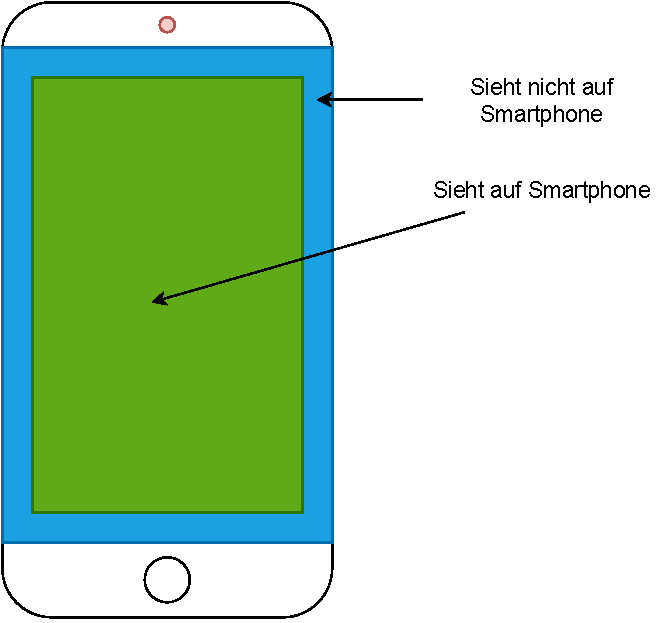
\includegraphics[width=0.5\linewidth]{concept/webgazer.drawio.pdf}
    \caption{Darstellung des Grenzwertes am Rand des Smartphones (blau). Fällt die Prognose in diese Zone, soll angenommen werden, dass die Person nicht auf das Smartphone sieht.}
    \label{fig:concept:webgazer:threshold}
\end{figure}

Doch bereits die ersten Tests mit dem neuen Prototypen haben gezeigt, dass dieser Ansatz bereits bei einem Laptop mit einem größeren Bildschirm als bei einem Smartphone nicht funktioniert. Wenn absichtlich nicht auf den Bildschirm gesehen wurde, waren die Vorhersagen sehr ungenau. Sie wurden nicht wie erwartet am Rand des Bildschirms angezeigt. Beispiele für solche Fehlerfälle sind in der Abbildung \ref{fig:concept:webgazer:wrong} zu sehen. Dasselbe Verhalten konnte bei dem Einsatz auf einem Smartphone beobachtet werden. 

\begin{figure}{}
    \begin{subfigure}{0.9\textwidth}
        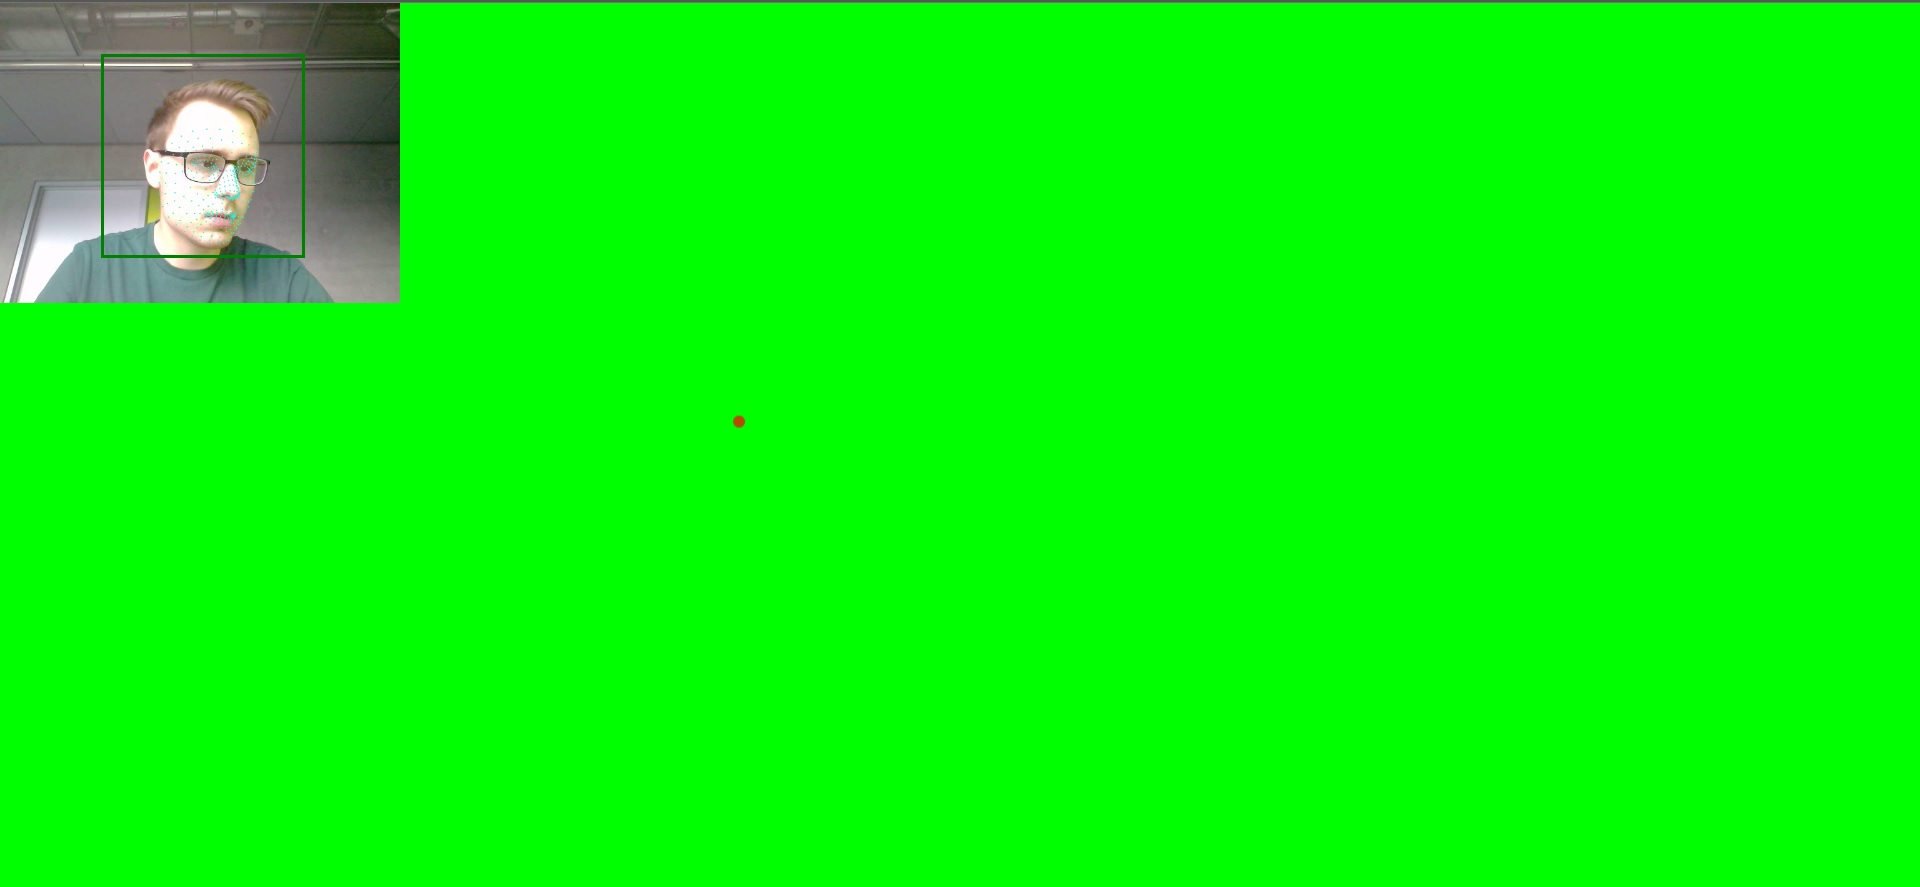
\includegraphics[width=\linewidth]{webgazer/webgazer_wrong_1.jpg}
    \end{subfigure}%
     \vspace{0.5cm} % Abstand zwischen den beiden Bildern
    \begin{subfigure}{0.9\textwidth}
        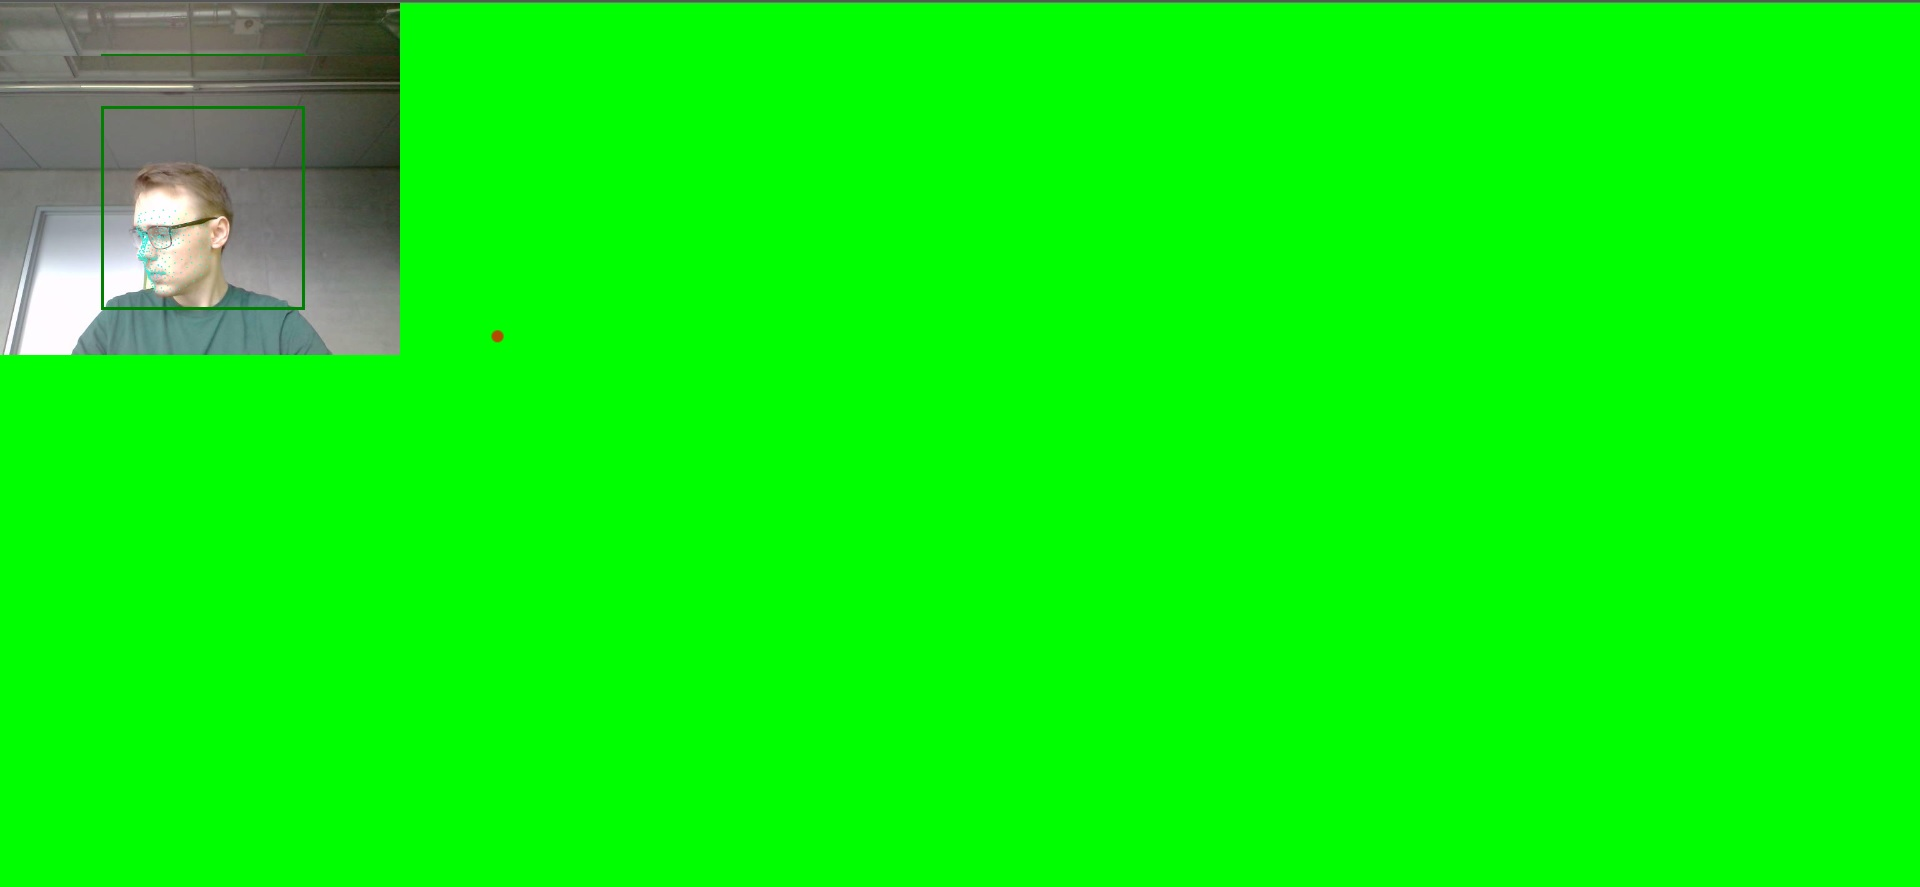
\includegraphics[width=\linewidth]{webgazer/webgazer_wrong_2.jpg}
    \end{subfigure}
    \caption{Beispiele für die Vorhersagen von WebGazer (roter Punkt), wenn eine Person nicht auf den Bildschirm sieht.}
    \label{fig:concept:webgazer:wrong}
\end{figure}

Somit kann mittels \textit{WebGazer} keine Aussage darüber getroffen werden, ob die Person auf das Smartphone schaut oder nicht. Daher ist ein solcher Ansatz für den Einsatz im Rahmen der PrioBike-App nicht geeignet, weshalb dieser Ansatz verworfen wurde. 

\section{Blickrichtungsbestimmung anhand der Kopfrotation}\label{sec:concept:head}

Ein weiterer in der Recherche identifizierter Ansatz besteht darin, die Blickrichtung von Radfahrenden anhand ihrer Kopfrotation zu bestimmen. Dieser Ansatz wird in der Arbeit von Henseler \cite{bachelor:henseler:gaze-ebikes} vorgestellt und in Kapitel \ref{sec:related:henseler} erläutert. Der Ansatz kann in mehrere Teilprobleme unterteilt werden. Zunächst muss das Gesicht des Radfahrenden im Bild erkannt werden. Anschließend müssen die Gesichtsmerkmale identifiziert werden. Abschließend erfolgt die Bestimmung der Kopfrotation anhand der erkannten Gesichtsmerkmale und eine Interpretation der Ergebnisse.  Die Umsetzung des von Henseler vorgestellten Ansatzes weist jedoch einige Probleme auf, die diese für den Einsatz im Rahmen der PrioBike-App ungeeignet machen. Die Umsetzung ist bezüglich der Lichtverhältnisse im Video sehr unflexibel. Zudem sind eine spezielle Smartphone-Halterung und eine Markierung am Fahrradhelm erforderlich. Außerdem treten die größten Ungenauigkeiten bei Henseler's Umsetzung auf, wenn es darum geht zu erkennen, wann die Person auf das Smartphone schaut.

Daher wurde untersucht, wie die Blickrichtung der Radfahrenden anhand der Kopfrotation robuster bestimmt werden kann. Es wurde festgestellt, dass das Thema der Gesichtserkennung und Gesichtsmerkmalsbestimmung in vielen verschiedenen Anwendungsbereichen von Bedeutung ist und daher bereits umfangreiche Forschung zu diesem Thema betrieben wurde, wie in Kapitel \ref{sec:related:face} erläutert wird. Dementsprechend gibt es auch einige Technologien, welche dafür entwickelt wurden, das Erkennen von Gesichtern und Gesichtsmerkmalen in Bildern zu ermöglichen. Um zu prüfen, ob diese Form der Gesichtserkennung für den Anwendungsfall der PrioBike-App geeignet ist, wurde ein Prototyp unter Verwendung von \textit{Google ML Kit}\footnote{\url{https://pub.dev/packages/google_ml_kit} (Abgerufen am 09.11.2023)} entwickelt. Diese Bibliothek wurde speziell für die Verwendung auf Smartphones entwickelt und ermöglicht das Lösen verschiedener Computer Vision Aufgaben mithilfe von maschinellem Lernen. So können mit \textit{Google ML Kit} Gesichter sowie eine Liste von Gesichtsmerkmalen in Form von zweidimensionalen Punkten erkannt werden. Ein Beispiel für das Ergebnis der Erkennung ist in Abbildung \ref{fig:concept:google_ml_kit} dargestellt.

\begin{figure}
    \centering
    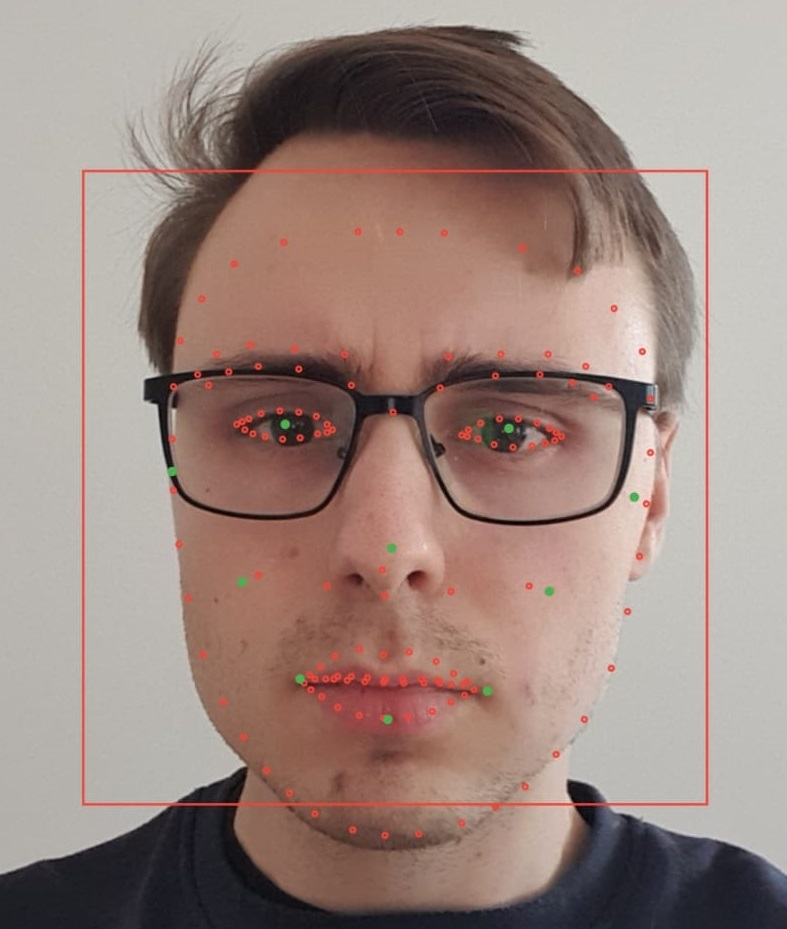
\includegraphics[width=0.5\linewidth]{concept/google_ml_kit.jpg}
    \caption{Erkannte Orientierungspunkte des Gesichts mit \textit{Google ML Kit}}
    \label{fig:concept:google_ml_kit}
\end{figure}

Mit diesem Prototypen wurden erste Tests durchgeführt, um den Einfluss von Licht, teilweise verdeckten Gesichtern und extremen Kopfrotationen auf die Qualität der Gesichtserkennung zu untersuchen. Es wurde festgestellt, dass die Erkennung auch bei sehr heller oder sehr dunkler Beleuchtung gut funktioniert. Es wurde auch kein Unterschied zwischen Personen mit und ohne Brillen festgestellt. Allerdings wurde beobachtet, dass die Qualität bei extremen Kopfrotationen, insbesondere entlang der Querachse, leicht nachgelassen hat. Insgesamt wurde dieser Ansatz der Gesichtserkennung jedoch als vielversprechend eingestuft.

\subsection{Betrachtung anhand Kopfrotation}

Nach der Erkennung der Gesichtsmerkmalen hat sich Henseler als nächstes mit der Bestimmung und Interpretation der Kopfrotation beschäftigt. Auch für dieses Problem bietet das \textit{Google ML Kit} eine Lösung, bei der anhand der erkannten Gesichtsmerkmale die Rotationswinkel entlang der Quer-, Längs- und Vertikalachse bestimmt werden können. Anhand dieser Werte soll nun entschieden werden, ob das Gesicht zum Smartphone orientiert ist oder nicht.

Dafür wurde der Prototyp weiterentwickelt. Es wurden experimentell Grenzwerte für die Rotationswinkel entlang der Quer- und Vertikalachse festgelegt. Wenn die erkannte Rotation bei einer der Achsen außerhalb dieser Grenzwerte liegt, wird davon ausgegangen, dass die dargestellte Person nicht auf das Smartphone schaut. Die Längsachse wurde dabei nicht berücksichtigt, da durch eine Rotation um diese Achse die generelle Orientierung des Gesichts zum Bildschirm unverändert bleibt. 

Dieser Ansatz hat gute Resultate bei einer ruhenden Person vor dem Bildschirm erzielt. Eine solche Person ist in der Abbildung \ref{fig:concept:google_vision:position:middle} zu sehen. Der Ansatz funktioniert jedoch nur, solange die Position des Kopfes im Bild konstant bleibt. In Abbildung \ref{fig:concept:google_vision:position:top} ist eine Person mit ähnlicher Kopfrotation wie in Abbildung \ref{fig:concept:google_vision:position:middle} zu sehen, allerdings ist zu erkennen, dass diese Person nicht auf das Smartphone sieht. Das zeigt, dass die ermittelten Grenzwerte von der Position und Größe des Kopfes im Bild abhängen. Aus diesem Grund müssten diese Grenzwerte je nach Position des Kopfes relativ zu Kamera angepasst und optimiert werden, da auf dem Fahrrad nicht gewährleistet werden kann, dass sich der Kopf immer in derselben Position im Bild befindet. Es muss daher eine andere Lösung gefunden werde, um die Kopfrotation zu interpretieren.

\begin{figure}[]
    \begin{subfigure}{0.35\textwidth}
        
\includegraphics[width=\linewidth]{concept/googlevision/google_vision_schaut.jpg}
        \caption{Nutzer schaut auf das Smartphone-Display}
        \label{fig:concept:google_vision:position:middle}
    \end{subfigure}\hspace{0.5cm}
    \begin{subfigure}{0.35\textwidth}
        
\includegraphics[width=\linewidth]{concept/googlevision/google_vision_schaut_nicht.jpg}
        \caption{Nutzer schaut nicht auf das Smartphone-Display}
        \label{fig:concept:google_vision:position:top}
    \end{subfigure}
    \caption{Darstellung der Auswirkung unterschiedlicher Kopfpositionen im Bild auf die Bedeutung der Kopfdrehung. Zweimal ist eine Person zu sehen, die fast keine Kopfdrehung aufweist. In Abbildung \ref{fig:concept:google_vision:position:middle} ist zu sehen, dass dies bedeutet, dass die Person auf das Smartphone schaut. In Abbildung \ref{fig:concept:google_vision:position:top} ist dieselbe Person mit derselben Kopfdrehung zu sehen. Es ist jedoch zu erkennen, dass die Person in diesem Bild nicht auf das Smartphone schaut.}
    \label{fig:concept:google_vision:position}
\end{figure}

\subsection{Dreidimensionale Betrachtung}\label{sec:concept:head:3d}

In einem neuen Ansatz wird die Entscheidung, ob eine Person auf das Smartphone schaut oder nicht, als dreidimensionales Problem betrachtet. Das Koordinatensystem des dreidimensionale Raumes wird dabei so konzipiert, dass die Kamera den Koordinatenursprung darstellt. Unter der Annahme, dass sich die Kamera in der Mitte des Bildes befindet, lässt sich die Position des Kopfes relativ zur Kamera anhand der zweidimensionalen Gesichtspunkte durch die x-Achse in der Breite und die y-Achse in der Höhe bestimmen. Allerdings ist die Tiefe $z$ dieser Punkte nicht bekannt. Da diese Gesichtspunkte im Sichtfeld der Kamera liegen, muss ihre Tiefe größer als null sein. Die Kamera liegt auf der dreidimensionalen Ebene $\cameraplane$, die durch $z = 0$ beschrieben werden kann. Da die Kamera fest im Smartphone integriert ist, hat auch das gesamte Display eine Tiefe von 0 und befindet sich damit ebenfalls auf derselben Ebene.
Wenn man annimmt, dass man die dreidimensionale Position eines Kopfes kennt, der sich direkt frontal vor der Kamera befindet und in keiner der Achsen rotiert wurde, kann man einen Richtungsvektor $\gazevector$ bestimmen, der parallel zur z-Achse und in Richtung der Ebene $\cameraplane$ verläuft. Dieser Richtungsvektor entspricht in diesem Fall der Blickrichtung des Kopfes. Mithilfe eines Punktes $\centerface$ des Kopfes und diesem Vektor $\gazevector$ lässt sich eine Gerade $G$ definieren, die orthogonal zur Ebene $\cameraplane$ verläuft und sie im Punkt $\intersection$ schneidet. 

Rotiert man diesen Kopf und entsprechend auch den Vektor $\gazevector$, dann verändert sich die Position des Schnittpunkts $\intersection$ auf der Ebene $\cameraplane$. Da das Display des Smartphones, wie bereits erwähnt, ebenfalls auf der Ebene $\cameraplane$ liegt, soll auf dieser Ebene $\cameraplane$ eine Zone definiert werden, die das Display des Smartphones repräsentiert. Wenn sich der Punkt $\intersection$ innerhalb dieser Zone befindet, sieht die dargestellte Person auf das Smartphone (siehe Abbildung \ref{fig:concept:head:example:yes}). Wenn sich der Punkt $\intersection$ außerhalb dieser Zone befindet, sieht die Person nicht auf das Smartphone (siehe Abbildung \ref{fig:concept:head:example:no}).

\begin{figure}[]
    \begin{subfigure}{0.8\textwidth}
        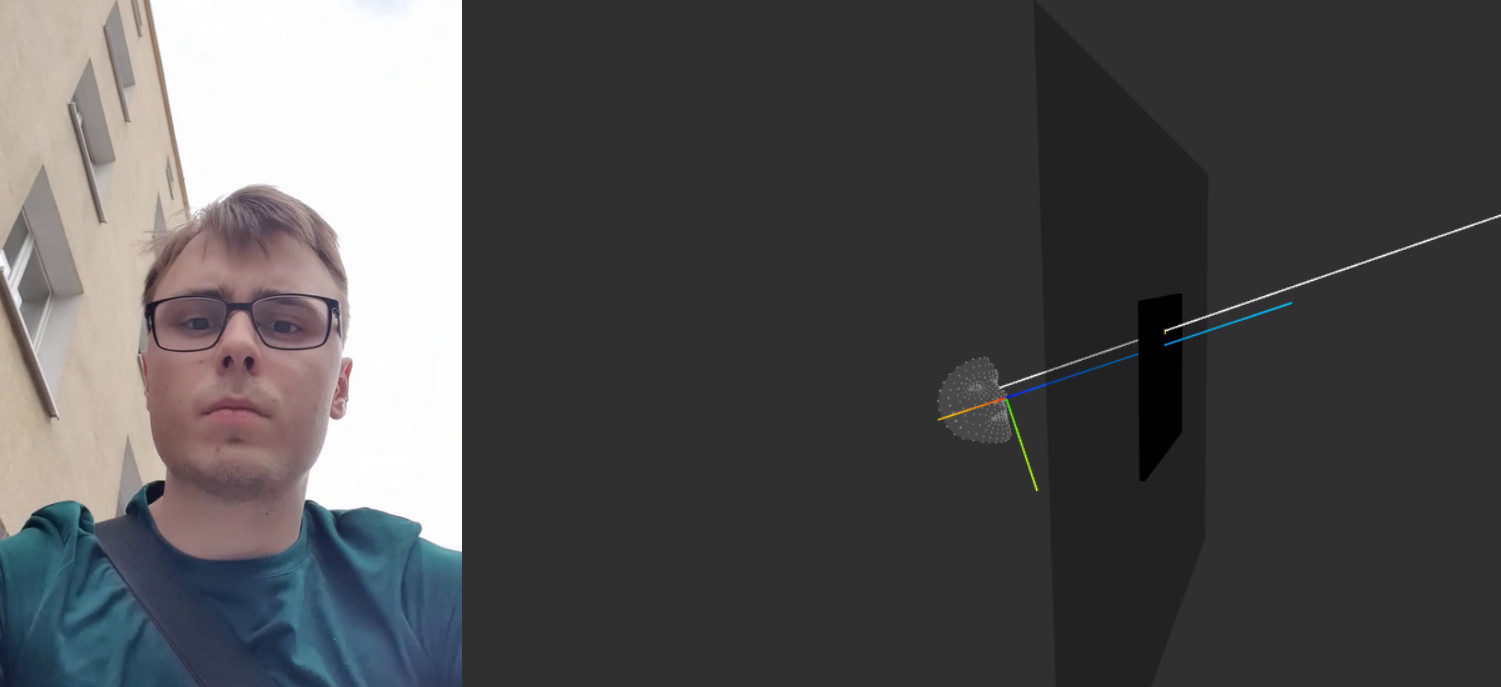
\includegraphics[width=\linewidth]{concept/concept_head_sieht.jpg}
        \caption{Person sieht auf Smartphone}
        \label{fig:concept:head:example:yes}
    \end{subfigure}
    \begin{subfigure}{0.8\textwidth}
        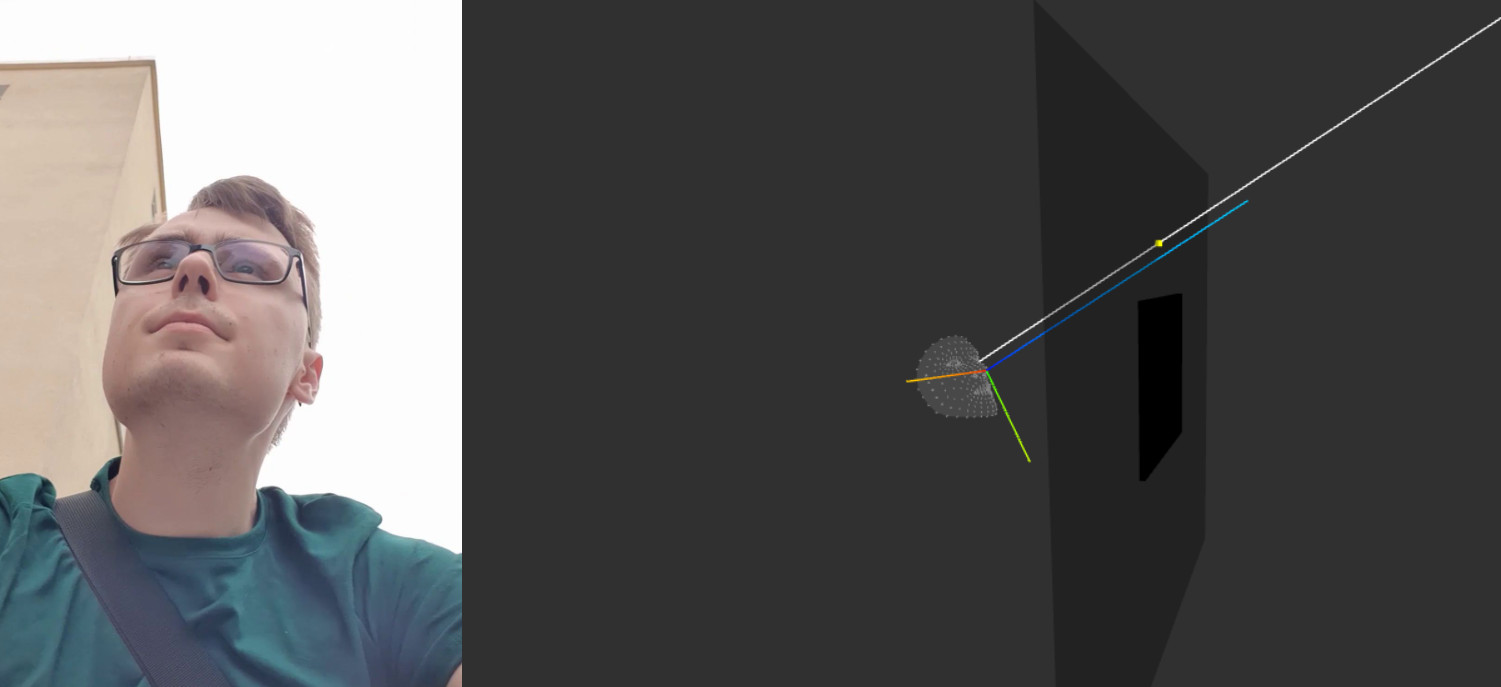
\includegraphics[width=\linewidth]{concept/concept_head_sieht_nicht.jpg}
        \caption{Person sieht nicht auf Smartphone}
        \label{fig:concept:head:example:no}
    \end{subfigure}
    \caption{Darstellung der dreidimensionalen Gesichtspunkte, der Ebene $\cameraplane$, der Geraden $G$, des Bereichs, der das virtuelle Smartphone-Display darstellt, und des entsprechenden Schnittpunkts $\intersection$.}
    \label{fig:concept:head:example}
\end{figure}

Über die Tiefe der einzelnen Gesichtspunkte gibt \textit{Google ML Kit} leider keine Aussage. Da der Abstand zwischen dem Kopf des Radfahrers je nach Körpergröße, Sitzhaltung und Fahrradtyp unterschiedlich ist, kann auch keine generelle Distanz geschätzt werden. 

Das Problem der Abbildung von zweidimensionalen Bildpunkten auf dreidimensionale Punkte wird als \textit{Pose Computation Problem} \cite{paper:pose:problem} bezeichnet. Dieses Problem wird unter anderem in der Arbeit von Zhang et al. über den \textit{ETH-XGaze} Datensatz diskutiert \cite{paper:eth-xgaze}. Zur Lösung dieses Problems nutzen sie ein spezielles dreidimensionales Modelle des Gesichts, das aus der gleichen Anzahl von Punkten bestehen wie die Anzahl der erkannten Gesichtsmerkmale. Zudem wird eine Abbildung verwendet, um zu ermitteln, welcher zweidimensionale Punkt zu welchem dreidimensionalen Punkt gehört. Anhand von diesem Modell lässt sich ein Rotationsvektor $\vec{r}$ und ein Translationsvektor $\vec{t}$ bestimmen. Diese geben an, wie das dreidimensionale Modell des Gesichts verformt und verschoben werden muss, um der durch die zweidimensionalen Bildpunkte gegeben Kopfposition zu entsprechen. Somit lässt sich aus den erkannten zweidimensionalen Punkten eine dreidimensionale Darstellung des Kopfes entwickeln, mit der der oben beschriebene Ansatz umgesetzt werden kann.

Auf dieser Grundlage wurde das erste Konzept für die Bestimmung der Blickrichtung in dieser Arbeit festgelegt. Hierfür sollen Videos von Radfahrenden mittels der Innenkamera des Smartphones unter verschiedenen Umweltbedingungen aufgenommen werden. Anschließend soll das Gesicht in den einzelnen Frames der Videos erkannt werden. Dafür sollen verschiedene Methoden zur Erkennung von Gesichtsmerkmalen verwendet werden, die in Kapitel \ref{sec:related:face} vorgestellt wurden. Mittels der dabei erkannten Gesichtspunkte soll im nächsten Schritt ein dreidimensionales Modell erstellt werden, mit dessen Hilfe dann die Gerade $G$ bestimmt wird, um den Schnittpunkt $\intersection$ mit der Ebene $\cameraplane$ zu finden. Anschließend soll untersucht werden, bei welchen dieser Schnittpunkte die Person auf das Smartphone gesehen hat, um so die beschriebene Zone auf der Ebene $\cameraplane$ zu bestimmen.

Um mögliche Fehlerquellen und Schwächen dieses Ansatzes zu untersuchen, soll die Erkennungsqualität der Gesichtsmerkmale evaluiert werden. Für eine quantitative Evaluation der erkannten Gesichtspunkte müssten für jedes aufgenommene Bild alle vorhandenen Gesichtspunkte manuell markiert werden \cite{paper:face:survey}. Leider ist dies im zeitlichen Rahmen dieser Arbeit nicht umsetzbar. Die Qualität der Gesichtserkennung soll daher subjektiv für jedes einzelne Bild eingeschätzt werden, was jedoch ebenfalls mit großem zeitlichem Aufwand verbunden ist. Aus diesem Grund können nicht alle in Kapitel \ref{sec:related:face} präsentierten Algorithmen in dieser Arbeit getestet werden.

Es wurde daher beschlossen, sich in erster Linie auf Gesichtserkennungsmethoden zu konzentrieren, die gut auf Smartphones genutzt werden können. Die Entscheidung fiel auf die Verwendung des \textit{Ensemble of Regression Trees (ERT)} und der Gesichtserkennungspipeline des \textit{MediaPipe} Frameworks. Diese Wahl wurde aufgrund der hohen Geschwindigkeit der Methoden und der Verfügbarkeit von Open-Source-Implementierungen getroffen.

Problematisch an diesem Ansatz ist, dass er darauf beruht, dass ein Gesicht und die entsprechenden Gesichtsmerkmale erkannt werden konnten. Daher stellt sich die Frage, ob eine Aussage darüber getroffen werden kann, ob die Person auf das Smartphone schaut oder nicht, obwohl kein Gesicht erkannt wurde. Wie bereits erwähnt, haben erste Tests mit dem Prototypen basierend auf \textit{Google ML Kit} gezeigt, dass vor allem eine starke Kopfdrehung zu Problemen bei der Gesichtserkennung geführt hat. Daher wird die Annahme getroffen, dass in den meisten Situationen, in welchen das Gesicht nicht identifiziert werden kann, dies auf die Rotation des Kopfes zurückzuführen ist. Weiter wird angenommen, dass wenn der Kopf extrem gedreht ist, sich das Smartphone am Lenker außerhalb des Blickfeldes der Person befindet und diese daher höchstwahrscheinlich nicht auf das Gerät schaut. Diese Annahme soll bei der Evaluation des Ansatzes untersucht werden. Wenn diese Annahme bestätigt werden kann, kann gesagt werden, dass wenn kein Gesicht erkannt wurde, die Person auch höchstwahrscheinlich nicht auf das Smartphone gesehen hat.

\subsection{MediaPipe}

Das in Kapitel \ref{sec:concept:head:3d} beschriebene Konzept basiert ausschließlich auf der Rotation und Position des Kopfes. Der große Nachteil dieses Ansatzes ist jedoch, dass die Blickrichtung der Augen nicht berücksichtigt wird, die das Ergebnis der Vorhersage noch weiter verfeinern könnte. Bei der Recherche wurde das Framework \textit{MediaPipe} \cite{paper:mediapipe} entdeckt, welches in Kapitel \ref{sec:related:mediapipe} vorgestellt wurde. Teil des Frameworks ist die \textit{FaceLandmarker}\footnote{\url{https://developers.google.com/mediapipe/solutions/vision/face_landmarker} (Abgerufen am 15.11.2023)} Pipeline. Mit dieser können neben dem Gesicht auch sogenannte \textit{Facial Blendshapes Scores} erkannt werden. Bei diesen Scores handelt es sich um einen Wert, der beschreibt, mit welcher Sicherheit einer von 52 Gesichtsausdrücken erkannt wird. Unter diesen Gesichtsausdrücken gibt es einige, die sich auf die Augen der erkannten Person beziehen. So gibt es für jedes Auge eine Score für den Blick nach links, nach rechts, nach oben und nach unten.

Basierend auf diesen augenbezogenen Scores wurde ein Ansatz entwickelt, um die Augenposition in den Vektor $\gazevector$ zu integrieren. Dazu sollte eine Abbildung zwischen den Scores und einem Blickrichtungsvektor $\vec{g'}$ bestimmt werden. Um diese Abbildung zu bestimmen, wurde testweise eine Person beim Radfahren mit der Innenkamera eines Smartphones gefilmt. Anschließend wurden mithilfe von \textit{MediaPipe} für jeden einzelnen Frame des Videos das Gesicht der Person und die damit verbundenen Gesichtsausdrücke erkannt und analysiert. Dabei wurde schnell bemerkt, dass bei zu großer Kopfrotation die Scores der Augen ungenaue und oft falsche Tendenzen angaben. Aus diesem Grund wurde dieser Ansatz verworfen und nicht weiterverfolgt.

\section{Dreidimensionale Blickrichtungsbestimmung mit Convolutional Neural Networks}\label{sec:concept:3d}

Der letzte zu untersuchende Ansatz zur Bestimmung der Blickrichtung von Radfahrern basiert auf Deep Learning Appearance Based Methoden, die eine dreidimensionale Blickrichtungserkennung ermöglichen, nachdem sich, wie in Kapitel \ref{sec:concept:2d} beschrieben, die zweidimensionalen Bildschirmkoordinaten als unzureichend erwiesen haben. Einen Überblick über die bisherige Forschung zu diesem Thema wird in Kapitel \ref{sec:related:gaze:appearance} gegeben. 

Dort werden einige Datensätze und Verfahren vorgestellt, mit denen die Blickrichtung aus dem Bild des Gesichts oder der Augen einer Person mittels eines Convolutional Neural Networks bestimmt werden kann.
Ein solche Methode soll nun auch in dieser Arbeit verwendet werden, um anhand der Innenkamera des Smartphones Bilder der Radfahrenden aufzunehmen, diese in ein Modell zu geben und dann eine Vorhersage der Blickrichtung zu erhalten.

Für das Training eines solchen Convolutional Neural Networks wurden in Kapitel \ref{sec:related:gaze:appearance} verschiedene Datensätze vorgestellt. Zunächst gibt es Datensätze mit zweidimensionalen Bildschirmpunkten als Ground Truth, wie zum Beispiel \textit{GazeCapture} \cite{paper:gazecapture} und \textit{TabletGaze} \cite{paper:tabletgaze}. Diese Datensätze sind daher, wie oben genannt, für die Verwendung in der PrioBike-App nicht geeignet. 

Die Arbeit von Zhang et al. \cite{paper:mpiifacegaze} hat gezeigt, dass die Blickrichtung mit solchen Methoden besser bestimmt werden kann, wenn das ganze Gesicht zur Vorhersage der Blickrichtung verwendet wird und nicht nur die Bilder der Augen. Dies ist insbesondere dann der Fall, wenn die Kopfdrehung oder die Lichtverhältnisse ungünstig sind, wie es beim Fahrradfahren häufig vorkommt. Außerdem kann die Kopfdrehung dazu führen, dass die Augen des Radfahrenden nicht mehr sichtbar sind. Die Grundlage für das Convolutional Neural Network sollte daher ein Datensatz sein, der Bilder von Gesichtern von Personen enthält.

Darüber hinaus sollte der Datensatz ein breites Spektrum an Kopfrotationen sowohl entlang der Querachse als auch entlang der Vertikalachse enthalten. Aus dem Blickwinkel der Innenkamera des Smartphones am Lenker ist die Kopfrotation entlang der Querachse sehr hoch, wenn die Person geradeaus entlang der Fahrtrichtung schaut. Bei einem Schulterblick oder sonstiger Verkehrsraumbeobachtung kann es zu hohen Kopfdrehungen entlang der Vertikalachse kommen. Außerdem müssen die verschiedenen Umwelteinflüsse, die sich auf die Bildqualität bei der Aufnahme während der Fahrt auswirken, durch den Datensatz kompensiert werden können. Es wurde daher entschieden, drei verschiedene Datensätze für das Training eines Convolutional Neural Networks auszuprobieren.

Der erste ausgewählte Datensatz ist der \textit{ETH-XGaze} Datensatz von Zhang et al. \cite{paper:eth-xgaze}. Dieser Datensatz zeigt die höchste Variation der Kopfdrehungen. Darüber hinaus wurden bei der Aufnahme des Datensatzes 16 verschiedene Lichtverhältnisse simuliert. Mit 110 abgebildeten Personen ist ein breites Spektrum menschlicher Vielfalt in diesem Datensatz enthalten.

Der zweite Datensatz, der verwendet werden soll, ist der \textit{Gaze360} Datensatz von Kellnhofer et al. \cite{paper:gaze360}. Dieser zeigt ebenfalls eine hohe Variation an Kopfrotationen und beinhaltet sowohl Innen- als auch Außenaufnahmen. Auch in diesem Datensatz ist mit 238 teilnehmenden Personen eine hohe Variation menschlicher Diversität enthalten.

Viele der anderen in Kapitel \ref{sec:related:gaze:appearance} vorgestellten Datensätze wurden mit der Webcam eines Laptops oder der Innenkamera eines Smartphones oder Tablets aufgenommen \cite{paper:mpiigaze, paper:gazecapture, paper:tabletgaze}. Für die Aufnahme dieser Datensätze mussten die Teilnehmenden einen Punkt auf dem Display ihres Geräts fixieren, um die Bilder mit der entsprechenden Blickrichtungen der Personen zu annotieren. Durch diese Methode sehen alle im Datensatz enthaltenen Personen auf das Display ihres Geräts. Dadurch wird einerseits die Variation der Kopfdrehung der Personen begrenzt. Andererseits sind dadurch keine Bilder im Datensatz enthalten, bei denen die Personen nicht auf das Gerät schauen. Da die Radfahrenden während der Fahrt großteils nicht auf das Smartphone schauen, ist davon auszugehen, dass solche Datensätze nicht für den Einsatz im Rahmen dieser Arbeit geeignet sind. Um das zu belegen, soll ein solcher Datensatz in die Untersuchung aufgenommen werden. Es wurde beschlossen, den \textit{MPIIGaze} \cite{paper:mpiigaze} Datensatz zu verwenden, insbesondere den \textit{MPIIFaceGaze} Datensatz, der die Bilder der Gesichter der Personen \cite{paper:mpiifacegaze} enthält. Es wurde sich für diesen Datensatz entschieden, da dieser Datensatz die dreidimensionale Blickrichtung der Person als Ground Truth besitzt. Darüber hinaus wurde der Datensatz während der alltäglichen Nutzung eines Laptops aufgenommen, wodurch eine hohe Variation verschiedener Umgebungsbedingungen repräsentiert wird.
 
In Kapitel \ref{sec:concept:head} wurde bereits ein Konzept zur Modellierung der Blickrichtung von Radfahrenden anhand der dreidimensionalen Kopfdrehung entwickelt. Mittels der mit den ausgewählten Datensätzen trainierten Convolutional Neural Networks kann nun die tatsächliche Blickrichtung einer Person als Vektor bestimmt werden. Dieser soll verwendet werden, um den Vektor, der nur auf der Kopfdrehung basiert, zu ersetzen, um anschließend wie in Kapitel \ref{sec:concept:3d} beschrieben einen Schnittpunkt $\intersection$ mit der Ebene $\cameraplane$ zu bestimmen.

Zusammengefasst besteht das Konzept darin, dass zunächst ein Bild des Radfahrenden mit der Innenkamera des Smartphones aufgenommen wird. Anschließend wird die in Kapitel \ref{sec:concept:head:3d} beschriebene Gesichtserkennung durchgeführt. Anhand der erkannten Gesichtspunkte wird das Gesicht des Radfahrenden aus dem Originalbild ausgeschnitten. Anschließend wird die dreidimensionale Kopfrotation und Kopfposition bestimmt. Dabei sollen verschiedene Störfaktoren bei der Blickrichtungsbestimmung eliminiert werden. Dafür soll das von Cheng et al. beschriebenen Verfahren zur Normalisierung \cite{paper:basics:survey} dieser Bilder verwendet werden. Dabei werden Störfaktoren wie der unterschiedliche Abstand zwischen Kamera und Gesicht oder die Drehung des Kopfes entlang der Längsachse, entfernt. Ein Beispiel für eine solche Normalisierung ist in Abbildung \ref{fig:concept:normalisation} dargestellt.

\begin{figure}[]
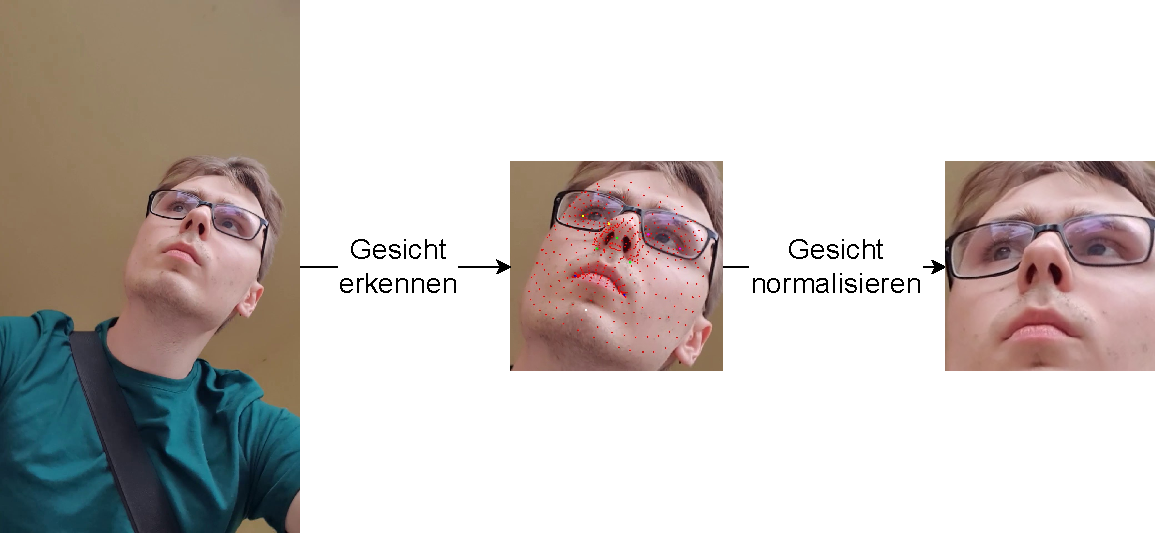
\includegraphics[width=\linewidth]{concept/normalisierung.drawio.pdf}
\caption{Beispielhafte Darstellung eines normalisierten Gesichts.}
\label{fig:concept:normalisation}
\end{figure}

Aus dem normalisierten Bild wird dann die Blickrichtung mithilfe von Convolutional Neural Networks vorhergesagt, die auf dem \textit{ETH-XGaze} \cite{paper:eth-xgaze}, \textit{Gaze360} \cite{paper:gaze360} und dem \textit{MPIIFaceGaze} \cite{paper:mpiifacegaze} Datensatz trainiert wurden. Das Ergebnis beschreibt dann die Blickrichtung des normalisierten Gesichts. Es muss daher wieder in das Koordinatensystem vor der Normalisierung transformiert werden, um die tatsächliche Blickrichtung $\gazevector$ zu erhalten. Mit dem Vektor $\gazevector$ wird dann zusammen mit der dreidimensionalen Position des Kopfes $\centerface$ eine Gerade $G$ entlang der Blickrichtung konstruiert. Mit $G$ wird dann der Schnittpunkt $\intersection$ mit der Ebene $\cameraplane$ bestimmt.  

Die Ergebnisse dieses Konzepts sollen dann genauso wie die Ergebnisse des Konzepts zur Bestimmung der Blickrichtung mittels der Kopfrotation evaluiert werden. Dafür wird für die entstandenen Schnittpunkte untersucht, bei welchen dieser Schnittpunkte die Person auf das Smartphone sieht, um so eine Zone auf der Ebene $\cameraplane$ zu bestimmen, die das Display des Smartphones repräsentiert (siehe Abbildung \ref{fig:concept:head:example}).

Bei vielen der im Kapitel \ref{sec:related:gaze} vorgestellten Datensätze wurden Bilder mit geschlossenen Augen bei der Datensatzerstellung aussortiert \cite{paper:eth-xgaze, paper:rt_gene, paper:tabletgaze}. Daher sollen auch in dieser Arbeit Bilder mit geschlossenen Augen identifiziert werden, um diese bei der Interpretation der Blickrichtung zu ignorieren.

Einen möglichen Ansatz für die Erkennung von geschlossenen Augen stellen Ibrahim et al. in ihrer Arbeit \cite{paper:ear} vor. Sie verwenden erkannte Gesichtspunkte rund um das Auge, um zu bestimmen, ob ein Auge offen (siehe Abbildung \ref{fig:concept:ear:open}) oder geschlossen (siehe Abbildung \ref{fig:concept:ear:closed}) ist. 

\begin{figure}[]
    \begin{subfigure}{0.45\textwidth}
        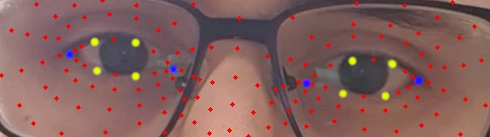
\includegraphics[width=\linewidth]{concept/ear-augen-offen.jpg}
        \caption{Augen geöffnet}
        \label{fig:concept:ear:open}
    \end{subfigure}%
    \vspace{0.5cm}
    \begin{subfigure}{0.45\textwidth}
        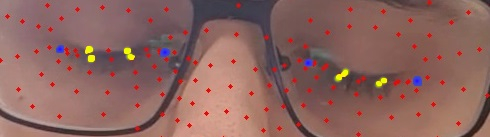
\includegraphics[width=\linewidth]{concept/ear-augen-zu.jpg}
        \caption{Augen geschlossen}
        \label{fig:concept:ear:closed}
    \end{subfigure}
    \begin{subfigure}{0.45\textwidth}
        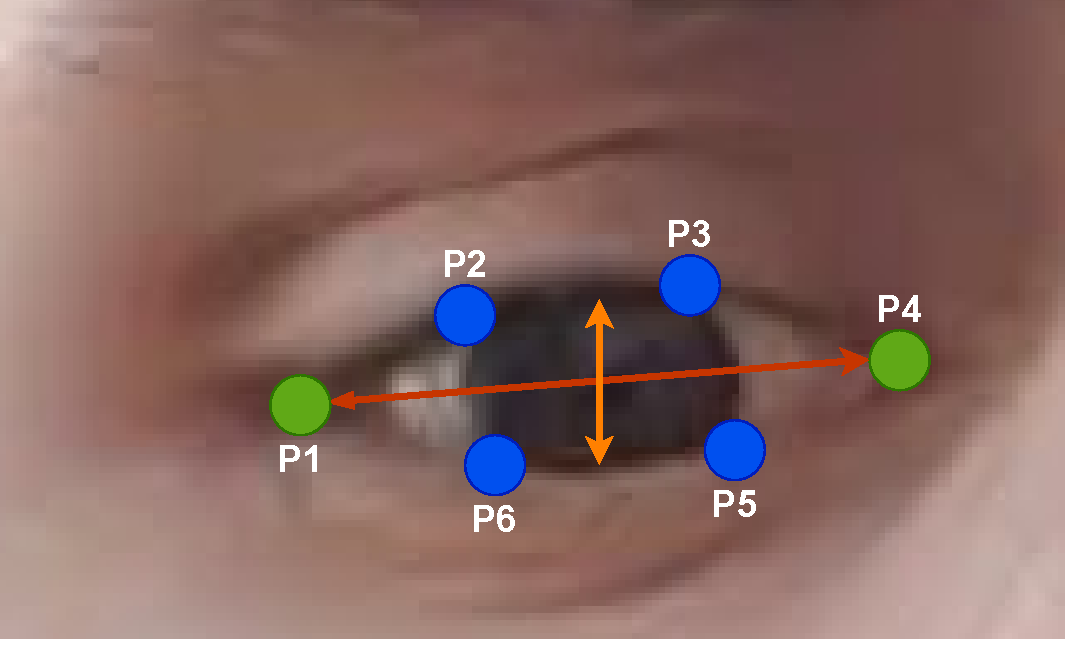
\includegraphics[width=\linewidth]{implementation/ear.drawio.pdf}
        \caption{Benötigte Punkte für die Berechnung des $EAR$}
        \label{fig:concept:ear:points}
    \end{subfigure}
    \caption{Erkennung von geschlossenen Augen anhand augenbezogener Gesichtspunkte.}
    \label{fig:concept:ear}
\end{figure}

Dazu wird das \textit{Eye Aspect Ratio} ($\ear$) berechnet. Dieser Wert errechnet sich aus sechs Punkten $P_1$ bis $P_6$ um das Auge herum. Die benötigten Punkte sind in Abbildung \ref{fig:concept:ear:points} dargestellt. Der Wert wird zunächst für jedes Auge einzeln mit folgender Formel berechnet:

\[
EAR_{\text{links/rechts}} = \frac{\|P_2 - P_6\| + \|P_3 - P_5\|}{2\|P_1 - P_4\|}
\]

Anschließend wird der Mittelwert aus beiden Werten gebildet. Dieser ergibt dann den endgültigen $EAR$-Wert.

\[
EAR = \frac{EAR_{\text{links}} + EAR_{\text{rechts}}}{2}
\]

Um nun zu entscheiden, ob eine Auge offen oder geschlossen ist, muss ein Grenzwert $\earthreshold$ festgelegt werden. Ist der berechnete Wert größer als $\earthreshold$, dann sind die Augen geöffnet. Wenn der Wert kleiner ist, sind die Augen geschlossen. Der ideale Grenzwert soll dabei während der Evaluation bestimmt werden.

\section{Zusammenfassung}

In diesem Kapitel wurden drei verschiedene Ansätze zur Bestimmung der Blickrichtung von Radfahrenden untersucht. 

Dabei hat sich gezeigt, dass Modelle, die für die Vorhersage von zweidimensionalen Bildschirmkoordinaten trainiert wurden, für die Anwendung im Rahmen der PrioBike-App nicht geeignet sind, da keine Aussage über die Blickrichtung der Radfahrenden getroffen werden kann, wenn diese nicht auf das Smartphone-Display schauen.

Weiter wurde untersucht, wie die Bestimmung der Blickrichtung anhand der Kopfrotation sowie mittels Convolutional Neural Networks in die PrioBike-App integriert werden kann. Dabei wurden zwei Konzepte entwickelt. In beiden Konzepten werden Radfahrende während der Fahrt mit der Innenkamera des Smartphones am Lenker gefilmt. Für die einzelnen Bilder dieser Videos wird anschließend eine Gesichtserkennung durchgeführt. Diese besteht aus dem Erkennen der Bounding Box des Gesichts, der Bestimmung von Gesichtspunkten in Form von zweidimensionalen Bildkoordinaten sowie der Bestimmung von der dreidimensionalen Position des Gesicht relativ zur Kamera.

Darauf aufbauend wird eine dreidimensionale Blickrichtung mit den beiden Konzepten auf unterschiedliche Weise bestimmt. Im ersten Konzept wird die dreidimensionale Drehung des Kopfes verwendet, um einen Vektor $\gazevector$ zu konstruieren, der die Blickrichtung der abgebildeten Person repräsentiert. Im zweiten Konzept werden Convolutional Neural Networks verwendet, um den Vektor $\gazevector$ zu bestimmen. Die Convolutional Neural Networks werden mit drei verschiedenen Datensätzen trainiert. Diese Datensätze sind \ethg \cite{paper:eth-xgaze}, \gazed \cite{paper:gaze360} und \mpii \cite{paper:mpiifacegaze}. 

Mithilfe des Vektors $\gazevector$ und der dreidimensionalen Position des Kopfes wird dann eine Gerade $G$ definiert. Mit $G$ wird ein Schnittpunkt $\intersection$ mit der Ebene $\cameraplane$ berechnet. Während der Auswertung wird untersucht, bei welchem dieser Schnittpunkte die Person auf das Smartphone geschaut hat, um einen Bereich auf der Ebene $\cameraplane$ zu definieren, der ein virtuelles Smartphone darstellt. Liegt ein Schnittpunkt $\intersection$ innerhalb dieses Bereichs, so hat die Person auf das Smartphone gesehen. Die Erkennung der Blickrichtung basiert auf den Ergebnissen der Gesichtserkennung. Wird kein Gesicht erkannt, kann der Vektor $\gazevector$ nicht bestimmt werden. Es wird davon ausgegangen, dass in den meisten Fällen ein nicht erkanntes Gesicht auf eine Drehung des Kopfes entlang der Querachse zurückzuführen ist. Da sich das Smartphone in diesem Fall nicht im Blickfeld der Person befindet, wird angenommen, dass die Person nicht auf das Smartphone schaut, wenn kein Gesicht erkannt wurde. Diese Annahme wird in der Evaluation überprüft.














  \chapter{Implementation}\label{sec:implementation}

In diesem Kapitel wird die Umsetzung der beiden in Kapitel \ref{sec:concept} erarbeiteten Konzepte vorgestellt. Dazu wird zunächst ein Überblick über den Stand der Implementierung gegeben. Anschließend wird die Umsetzung der einzelnen Teilschritte wie die Gesichtserkennung und die darauf aufbauende Blickrichtungsbestimmung vorgestellt.

\section{Übersicht}

Das Ziel der Implementierung ist die Analyse der Blickrichtung von Radfahrenden anhand der vorgestellten Konzepte, um Rückschlüsse zu ziehen, wann die Radfahrenden auf ihr Smartphone sehen. Dazu werden Videos mit der Frontkamera des Smartphones aufgenommen. Das Smartphone wird während der Fahrt am Lenker des Fahrrads befestigt.

Der grundlegende Ablauf der beiden Konzepte ist ähnlich. Zunächst erfolgt die Zerlegung der Videos in ihre einzelnen Teilbilder. Anschließend wird eine Gesichtserkennung als Grundlage für beide Konzepte durchgeführt. Das Ergebnis ist eine Liste der im Bild erkannten Gesichtspunkte, die sowohl als zweidimensionale Koordinaten als auch als dreidimensionale Position relativ zur Kamera angegeben werden. Da beide Konzepte auf den Ergebnissen der Gesichtserkennung basieren, wurde dieser Schritt separat von der restlichen Verarbeitung der Videos implementiert. Die Umsetzung des Prozesses wird in Kapitel \ref{sec:implementation:face} erläutert.

Der wesentliche Unterschied zwischen den beiden erarbeiteten Konzepten besteht darin, wie der Vektor ermittelt wird, der die Blickrichtung der Radfahrenden angibt. Die Interpretation dieser Blickrichtungen ist jedoch für beide Konzepte gleich.
Daher wird die Blickrichtungsbestimmung der beiden Konzepte separat voneinander durchgeführt. Die Interpretation der Ergebnisse erfolgte dann in einem gemeinsamen Schritt. Die spezifischen Details zur Implementierung der Blickrichtungsbestimmung werden in Kapitel \ref{sec:implementation:gaze} erläutert.

Die Umsetzung der Konzepte erfolgt mittels der Programmiersprache Python. Ein Überblick über die Struktur der Implementierung ist in Abbildung \ref{fig:implementation:uml} zu sehen. Für mathematische Berechnungen in dieser Arbeit wird zu großen Teilen die Python Bibliothek \textit{NumPy}\footnote{\url{https://numpy.org/} (Abgerufen am 29.11.2023)} verwendet.

\begin{figure}[]
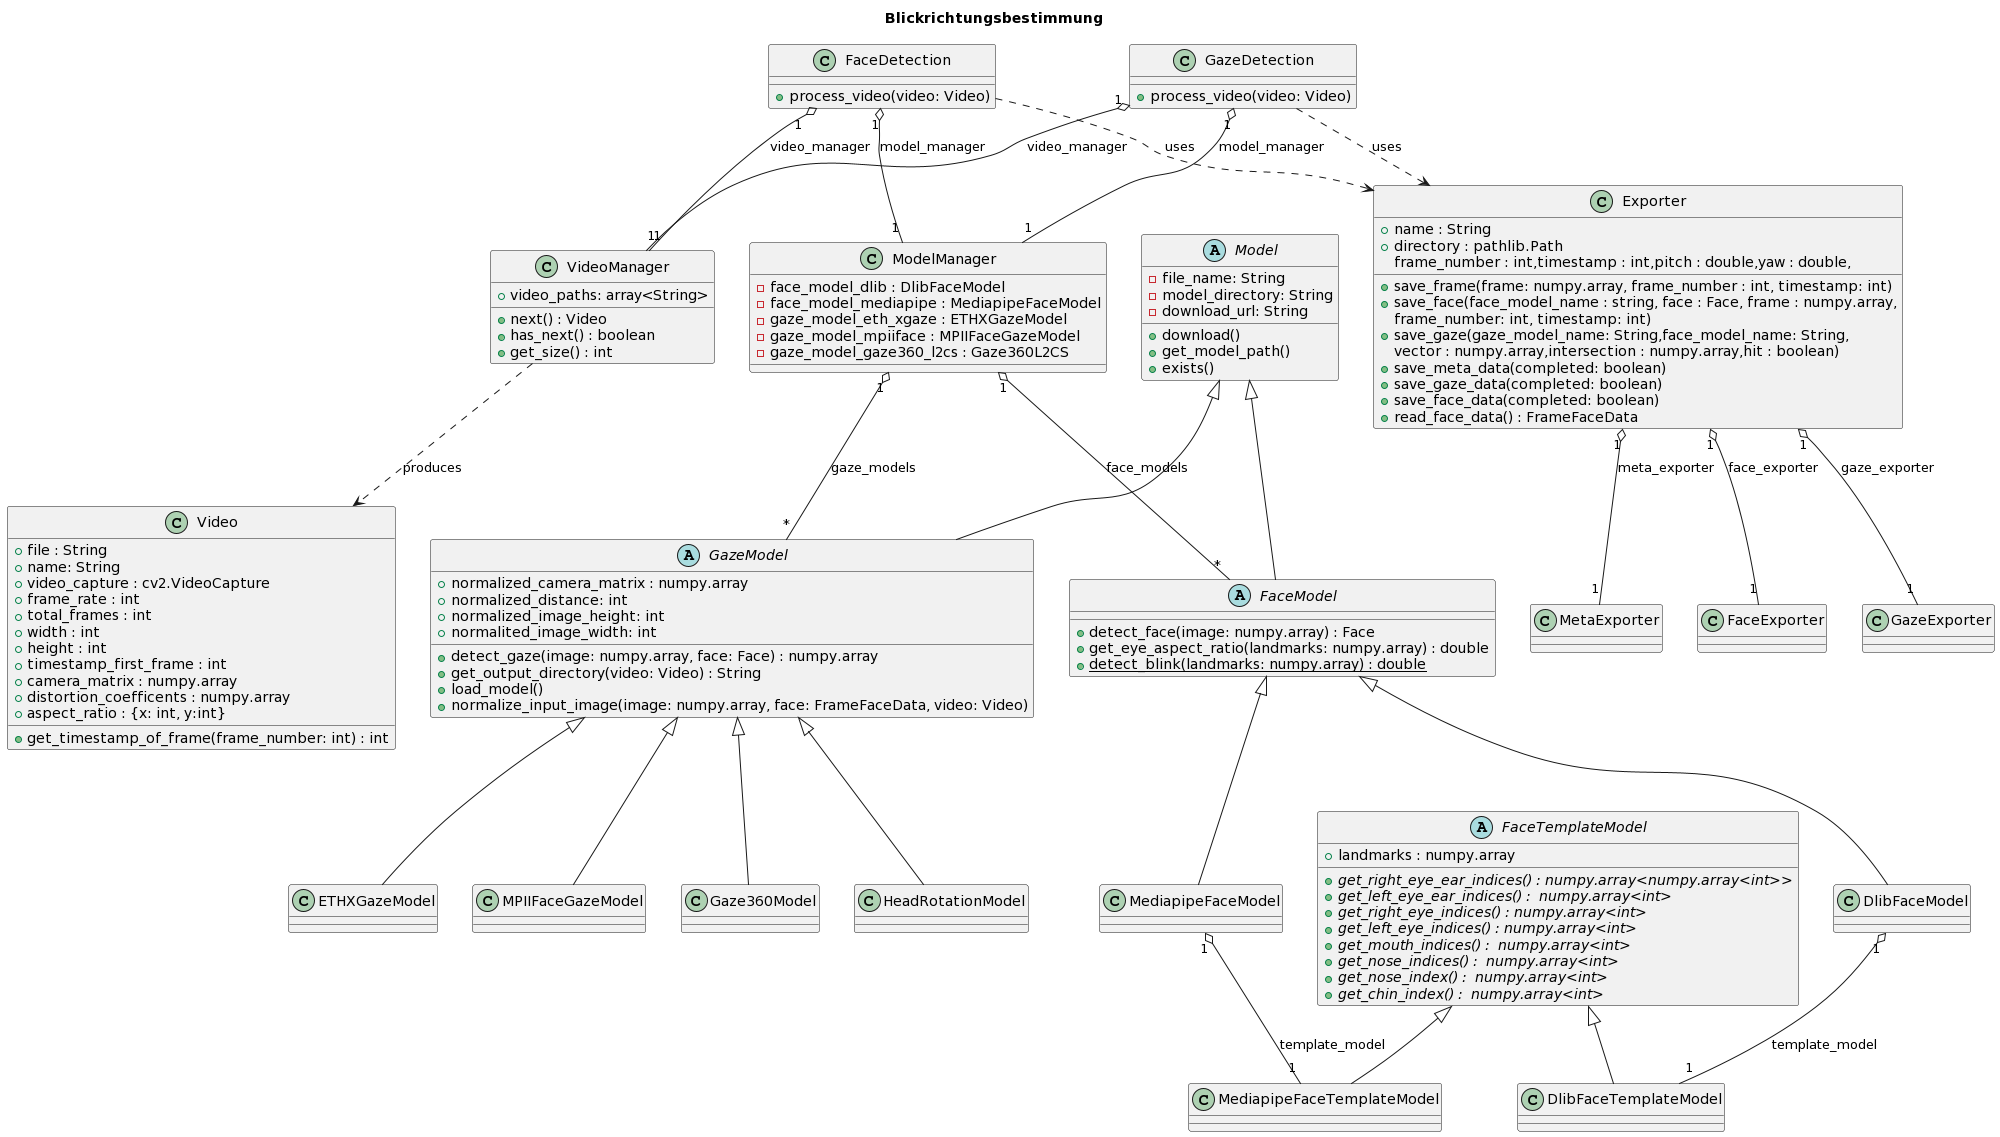
\includegraphics[width=\linewidth]{implementation/uml.png}
\caption{UML-Klassendiagramm\protect\footnote{Erstellt mit \url{https://www.planttext.com/} (Abgerufen am 09.11.2023)} des aktuellen Stands der Implementierung.}
\label{fig:implementation:uml}
\end{figure}

\section{Verarbeitung der Videos}\label{sec:implemenation:video}

Im ersten Schritt werden die Videos, die analysiert werden sollen, in die einzelne Frames der Videos zerlegt. Zudem werden weitere Details der Videos ermittelt, wie die Gesamtzahl der Frames eines Videos, die Anzahl der Frames pro Sekunde sowie die Höhe $\heightvideo$ und Breite $\widthvideo$ der Frames in Pixeln. Dafür wird die Python-Bibliothek von OpenCV\footnote{\url{https://github.com/opencv/opencv-python}  (24.10.2023)} \cite{paper:opencv} genutzt, welche Algorithmen für die Verarbeitung von Bildern und Videos bereitstellt. 

In der aktuellen Implementierung werden nur Videos im MP4-Format unterstützt, da bei der Aufnahme der Videos ausschließlich dieses Format verwendet wurde. OpenCV unterstützt jedoch eine Vielzahl von verschiedenen Videoformaten, wodurch bei Bedarf weitere Formate hinzugefügt werden können.

Anschließend werden die einzelnen Frames des Videos mithilfe von OpenCV iteriert. In der aktuellen Implementierung wird jedoch nur jeder dritte Frame verarbeitet, um den Aufwand während der Evaluation zu minimieren. Für jeden Frame $f$ wird dabei die Nummer $n$ sowie der Zeitpunkt des Frames $t$ in Millisekunden relativ zum Beginn des Videos bestimmt. Für die spätere Auswertung werden in diesem Schritt die ausgewählten Frames des Videos als Bild in einer separaten Datei gespeichert.  

\section{Erkennung und Verarbeitung von Gesichtsmerkmalen}\label{sec:implementation:face}

Für die in Kapitel \ref{sec:implemenation:video} ausgewählten Frames wird dann die Gesichtserkennung durchgeführt. Die Umsetzung von diesem Schritt wird in diesem Kapitel vorgestellt. Der generelle Ablauf der Gesichtserkennung ist in Abbildung \ref{fig:implementation:process:video} zu sehen.

\begin{figure}
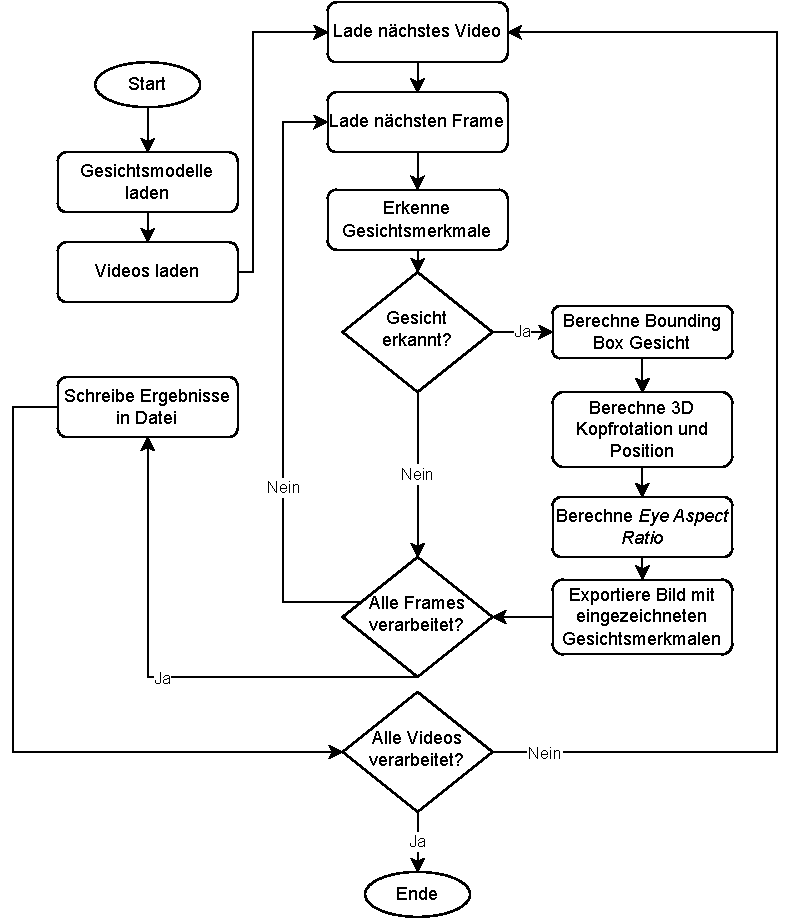
\includegraphics[width=0.5\linewidth]{implementation/process-face.pdf}
\caption{Ablauf der Gesichtserkennung.\protect\footnote{Erstellt mit \url{https://app.diagrams.net/} (Abgerufen am 09.11.2023)}}
\label{fig:implementation:process:video}
\end{figure}

\subsection{Identifizieren der Gesichtsmerkmale}\label{sec:implementation:face:landmarks}

Zunächst müssen die Gesichtsmerkmale der Radfahrenden identifiziert werden.
In Kapitel \ref{sec:concept:head} wurde festgelegt, dass zwei verschiedene Algorithmen zur Erkennung der Gesichtsmerkmale verwendet werden. Dabei handelt es sich um den \textit{ERT} Algorithmus \cite{paper:dlib} und die Gesichtserkennungspipeline von \mediapipe \cite{paper:mediapipe,paper:mediapipe:landmarks,paper:mediapipe:blazeface,paper:mediapipe:attention}.

Um den \textit{ERT} Algorithmus zu verwenden, wird die Implementierung des Algorithmus in der Open-Source Python Bibliothek\footnote{\url{https://pypi.org/project/dlib/} (Abgerufen am 21.08.2023)} von \dlib \cite{paper:dlib:main, paper:dlib} genutzt. Für die Erkennung von Gesichtsmerkmalen mit dem \mediapipe Framework wird das Python Package\footnote{\url{https://pypi.org/project/mediapipe/} (Abgerufen am 21.08.2023)} von \mediapipe verwendet.


Ziel ist nun eine Liste von einzelnen zweidimensionalen Gesichtspunkten $\landmark$ zu bestimmen, wobei $\indexlandmark$ den entsprechenden Index des Punktes in der Liste darstellt.
Das Erkennen der Gesichtsmerkmalen mit den beiden Methoden wird im Folgenden erläutert.

\subsubsection{MediaPipe}\label{sec:implementation:face:landmarks:mediapipe}

Für die Erkennung von Gesichtsmerkmalen mit \mediapipe wird die Klasse \textit{FaceMesh}\footnote{\url{https://github.com/google/mediapipe/blob/master/mediapipe/python/solutions/face_mesh.py} (Abgerufen am 21.11.2023)} des Frameworks verwendet.  Diese kombiniert den Schritt der Gesichtserkennung innerhalb des Bildes mit der Erkennung von insgesamt 468 Gesichtspunkten. Ein Beispiel für ein Bild mit erkannten Gesichtsmerkmalen ist in Abbildung \ref{fig:implementation:landmarks:mediapipe} zu sehen.

Die Klasse \textit{FaceMesh} kann über verschiedene Parameter konfiguriert werden. Zunächst kann festgelegt werden, ob das angezeigte Bild als einzelnes statisches Bild betrachtet werden soll oder ob das Bild Teil eines Videos ist und somit in Beziehung zu den vorhergehenden Bildern steht. Es wurde entschieden, das Bild einzeln zu betrachten. Dies wurde gemacht, da bei ersten Tests festgestellt wurde, dass sich ein Fehler bei der Gesichtserkennung sonst über mehrere Bilder erstreckt und immer nur stückweise korrigiert wird, um einen angenehmen Übergang beim Betrachten des Videos zu schaffen.
Darüber hinaus bietet \mediapipe mit dem Parameter \textit{refine\_landmarks} die Möglichkeit, die erkannten Punkte an markanten Stellen des Gesichts, zum Beispiel um das Auge und den Mund, weiter zu verfeinern \cite{paper:mediapipe:attention}. Dabei werden zusätzlich zehn weitere Gesichtspunkte zu den bereits erkannten hinzugefügt, welche die Iris der beiden Augen des Menschen darstellen. Es wurde sich dazu entschieden diese Verfeinerung der Gesichtspunkte durchzuführen. Die dabei zusätzlich erkannten Gesichtsmerkmale werden jedoch verworfen, da sie für die weitere Betrachtung der Gesichtserkennung ohne Bedeutung sind.
Weiterhin kann die erforderliche Zuversicht des Modells für die erfolgreiche Erkennung des Gesichts und der Gesichtsmerkmale konfiguriert werden. Diese wird als Wert zwischen 0 und 1 angegeben und ist standardmäßig auf 0,5 eingestellt. Bei Tests wurde jedoch festgestellt, dass die Standardzuversicht zu gering ist, da die Drehung des Kopfes des Radfahrenden häufig zu falsch erkannten Gesichtern geführt hat. Durch Ausprobieren wurde die erforderliche Mindestzuversicht des Modells für beide Erkennungen auf 0,8 festgelegt. Es ist jedoch anzumerken, dass keine Aussage darüber getroffen werden kann, welche Konfiguration für den Anwendungsfall in der PrioBike-App wirklich ideal ist, da die Qualität der Gesichtsmerkmalsbestimmung, wie bereits in Kapitel \ref{sec:concept:head} erwähnt, nur mit sehr großem Aufwand bewertet werden kann. Entweder man markiert für jedes Bild manuell die tatsächlichen Gesichtsmerkmale im Bild, um eine Ground Truth zu erstellen, was im zeitlichen Rahmen dieser Arbeit leider nicht umsetzbar war, oder ein Mensch klassifiziert die Qualität manuell durch das Betrachten der erkannten Gesichtsmerkmale jedes Mal neu, sobald man einen der Parameter angepasst hat, was im zeitlichen Rahmen dieser Arbeit ebenfalls nicht umsetzbar war.

Mit \mediapipe kann eine Liste von 468 einzelnen Gesichtsmerkmalen $\landmark$ in Form von dreidimensionalen Punkten, bestehend aus $\landmarkxnorm$, $\landmarkynorm$ und $\landmarkznorm$, ermittelt werden. $\landmarkxnorm$ gibt die normierte Position entlang der Breite des Bildes $\widthvideo$ an, $\landmarkynorm$ die normierte Position entlang der Höhe des Bildes $\heightvideo$. Die Koordinate $\landmarkznorm$ gibt einen normierten Tiefenwert für jeden Punkt an. Wie in Kapitel \ref{sec:concept:head:3d} beschrieben, soll aus den zweidimensionalen Bildkoordinaten eines Gesichtspunktes auf einen dreidimensionalen Gesichtspunkt relativ zur Kamera geschlossen werden. Mit dieser Methode liegen bereits dreidimensionale Punkte vor. Um jedoch eine bessere Vergleichbarkeit der beiden Methoden zur Bestimmung der Gesichtsmerkmale zu ermöglichen, soll die dreidimensionale Lage der Punkte auf die gleiche Weise bestimmt werden, weshalb die von \mediapipe bestimmte Tiefe der Punkte nicht weiter verwendet wird. Für mögliche zukünftige Experimente werden die Koordinaten jedoch gespeichert.

Für die in Kapitel \ref{sec:implementation:face:3d} beschriebene dreidimensionale Positionsbestimmung werden die Bildkoordinaten der Gesichtspunkte in Pixeln benötigt, weshalb die normierten Werte in Bildkoordinaten $\landmarkxbild$, $\landmarkybild$ umgerechnet werden.
 
\[
\landmarkxbild = \landmarkxnorm \cdot \widthvideo \qquad \landmarkybild = \landmarkynorm \cdot \heightvideo
\]

\subsubsection{dlib}

Um mit \dlib Gesichtspunkte zu bestimmen, muss zunächst im Bild ein Gesicht erkannt werden. Dafür wird der von \dlib Bibliothek bereitgestellte \textit{Face Detector} verwendet \cite{paper:dlib:face}. Die erkannten Gesichter liegen dann in Form einer Bounding Box vor. Anschließend wird mittels des von \dlib\footnote{\url{http://dlib.net/files/shape_predictor_68_face_landmarks.dat.bz2} (Abgerufen am 24.08.2023)} bereitgestellten \textit{Shape Predictors} 68 verschiedene Gesichtsmerkmale im Bild erkannt, welche in Form einer Liste von zweidimensionalen Bildkoordinaten $\landmarkxbild$ und $\landmarkybild$ vorliegen. Ein Beispiel für diese 68 erkannten Gesichtspunkte sind in Abbildung \ref{fig:implementation:landmarks:dlib} zu sehen.

Da die Koordinaten der Gesichtspunkte bei \mediapipe sowohl in normalisierter Form als auch in Bildkoordinaten vorliegen, wurden die Koordinaten $\landmarkxbild$ und $\landmarkybild$ aus Konsistenzgründen ebenfalls in die zweidimensionalen Koordinaten $\landmarkxnorm$, $\landmarkynorm$ umgewandelt. Wie bereits im Kapitel \ref{sec:implementation:face:landmarks:mediapipe} erläutert, wird die durch \mediapipe ermittelte Tiefe in Form der $\landmarkznorm$ Koordinate zwar nicht verwendet, aber dennoch gespeichert. \textit{Dlib} kann keine Auskunft über die Tiefe der Gesichtspunkte geben. Aus Konsistenzgründen wird aber ein Wert für $\landmarkznorm$ gespeichert werden. Dieser wurde für alle Gesichtspunkte auf 1 gesetzt. 

\[
\landmarkxnorm = \frac{\landmarkxbild}{\widthvideo} \qquad \landmarkynorm = \frac{\landmarkybild}{\heightvideo} \qquad \landmarkznorm = 1
\]


\begin{figure}[]
    \begin{subfigure}{0.425\textwidth}
        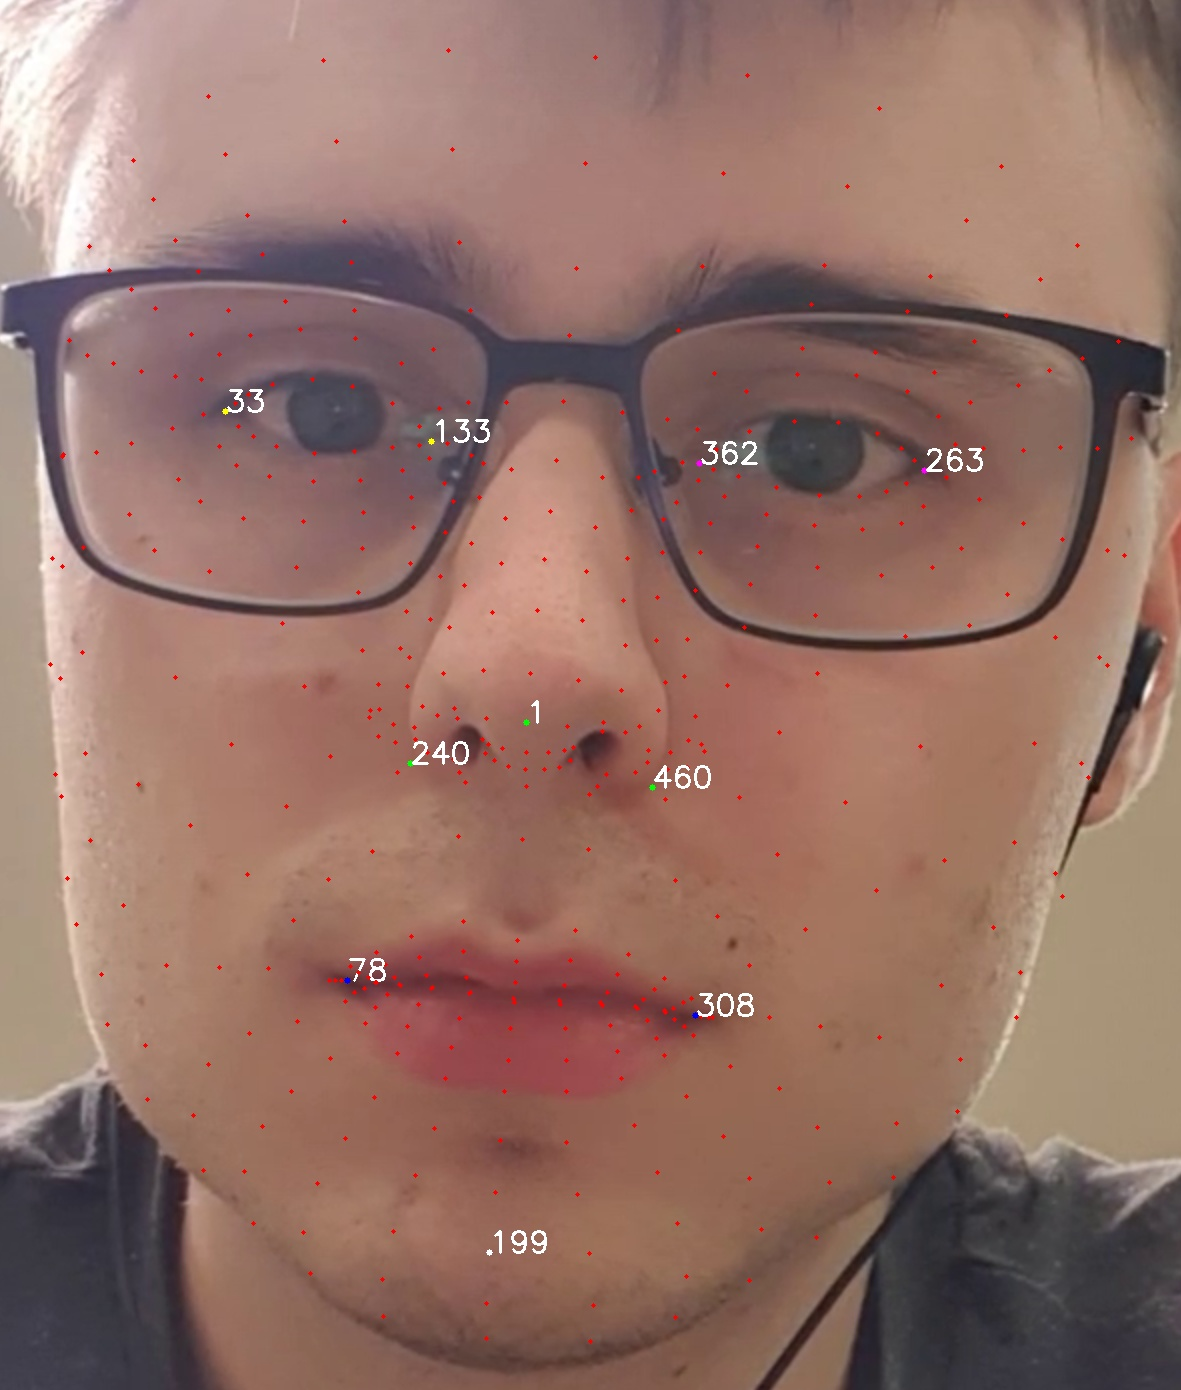
\includegraphics[width=\linewidth]{implementation/mediapipe.jpg}
        \caption{Beispiel von 468 Gesichtsmerkmalen mit \mediapipe}
        \label{fig:implementation:landmarks:mediapipe}
    \end{subfigure}%
    \hspace{0.5cm}
    \begin{subfigure}{0.475\textwidth}
        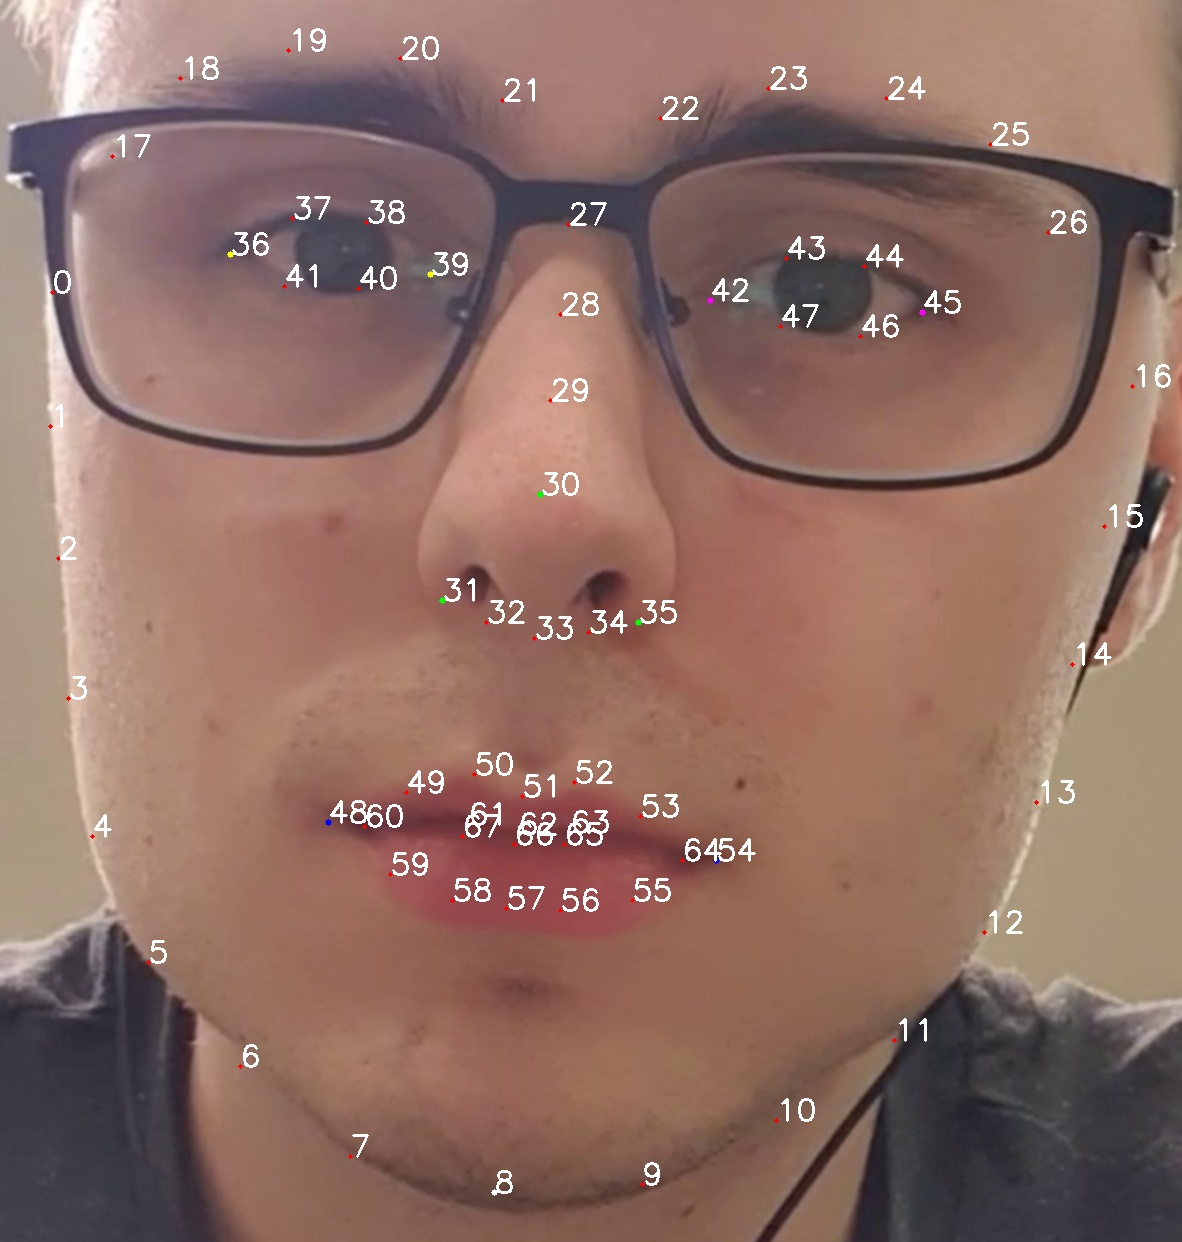
\includegraphics[width=\linewidth]{implementation/dlib.jpg}
        \caption{Beispiel von 68 Gesichtsmerkmalen mit der \dlib Bibliothek}
        \label{fig:implementation:landmarks:dlib}
    \end{subfigure}
    \caption{Beispiele für erkannte Gesichtsmerkmale mit \mediapipe und \dlib. Diese Gesichtsmerkmale sind anhand ihres Index $\indexlandmark$ beschriftet. In Abbildung \ref{fig:implementation:landmarks:mediapipe} sind aus Gründen der Übersichtlichkeit nur die wichtigsten Gesichtsmerkmale nummeriert.}
    \label{fig:implementation:landmarks}
\end{figure}

\subsection{Identifizieren von geschlossenen Augen}\label{sec:implementation:gaze:ear}

Aus den ermittelten zweidimensionalen Koordinaten $\landmarkxbild$ und $\landmarkybild$ eines Bildpunktes $\landmark$ wird nun das im Kapitel \ref{sec:concept:3d} beschriebene Verfahren zur Erkennung geschlossener Augen \cite{paper:ear} implementiert. Bei diesem Verfahren wird das \textit{Eye Aspect Ratio} ($EAR$) berechnet. Dazu werden sechs Punkte $P_1$ bis $P_6$ um das linke und rechte Auge benötigt. Die dafür verwendeten Gesichtsmerkmale $\landmark$ von \mediapipe und \dlib sind in Tabelle \ref{tab:implementation:ear} dargestellt.

\[
\ear_{\text{links/rechts}} = \frac{\|P_2 - P_6\| + \|P_3 - P_5\|}{2\|P_1 - P_4\|} \qquad \ear = \frac{\ear_{\text{links}} + \ear_{\text{rechts}}}{2}
\]

Anschließend muss ein Grenzwert $\earthreshold$ ermittelt werden. Ist der ermittelte $\ear$ Wert größer als $\earthreshold$, dann sind die Augen geöffnet. Wenn der Wert kleiner ist als $\earthreshold$, sind die Augen geschlossen. Dieser Grenzwert $\earthreshold$ wurde in der Evaluation für \dlib und \mediapipe bestimmt. Für \dlib beträgt der Wert 0,173 und für \mediapipe 0,159. Näheres dazu wird in Kapitel \ref{sec:evaluation:results:gaze:ear} erläutert.

\begin{table}[]
    \centering
    \begin{tabular}{c | c c | c c}
        \toprule
        & \multicolumn{2}{c|}{\textbf{dlib}} &\multicolumn{2}{c}{\textbf{MediaPipe}} \\
        \midrule
        \textbf{Punkt} & Linkes Auge & Rechtes Auge & Linkes Auge & Rechtes Auge \\
        \midrule
        $P_1$ & 42 & 36 & 362 & 33 \\
        $P_2$ & 43 & 37 & 385 & 160 \\
        $P_3$ & 44 & 38 & 387 & 158 \\
        $P_4$ & 45 & 39 & 263 & 133 \\
        $P_5$ & 46 & 40 & 373 & 153 \\
        $P_6$ & 47 & 41 & 380 & 144 \\
        \bottomrule
    \end{tabular}
    \caption{Verwendete Gesichtsmerkmale zur Bestimmung des $\ear$. Siehe Abbildung \ref{fig:implementation:landmarks}.}
    \label{tab:implementation:ear}
\end{table}

\subsection{Exportieren der Bilder mit erkannten Gesichtsmerkmalen}\label{sec:implementation:face:export:landmarks}

Wie in Kapitel \ref{sec:concept:head} beschrieben, soll die Gesichtserkennung in der Evaluation durch einen Menschen qualitativ beurteilt werden. Um diese Beurteilung zu ermöglichen, werden die zweidimensionalen Bildkoordinaten $\landmarkxbild$ und $\landmarkybild$ mittels der OpenCV-Bibliothek farblich markiert. Zusätzlich wird anhand dieser Punkte eine Bounding Box um das Gesicht berechnet, mit der das Bild auf das Gesicht zugeschnitten wird. Um die Beurteilung der Gesichtspunkte für einen Menschen zu erleichtern, werden markante Gesichtspunkte an Augen, Nase, Mundwinkel und Kinn farblich hervorgehoben. Die dafür verwendeten Gesichtsmerkmale sind in der Tabelle \ref{tab:implementation:used:landmarks} aufgeführt.
 
\begin{table}[]
    \centering
    \begin{tabular}{l c c }
    \toprule
        \textbf{Gesichtsmerkmal} & \textbf{dlib} & \textbf{MediaPipe} \\ \midrule
        Linkes Auge & 36, 39 & 33, 133 \\
        Rechtes Auge & 42, 45 & 263, 362 \\
        Mund & 48, 54 & 78, 308 \\
        Nase & 31, 35& 240, 460\\
        Nasenspitze & 30 & 1 \\
        Kinn & 8 & 199\\
        \bottomrule
    \end{tabular}
    \caption{Farblich hervorgehobene Gesichtspunkte für die Evaluation der erkannten Gesichtsmerkmale.}
    \label{tab:implementation:used:landmarks}
\end{table}

\subsection{Dreidimensionale Kopfrotation bestimmen}\label{sec:implementation:face:3d}

Wie in Kapitel \ref{sec:concept:head:3d} beschrieben, wird für die weitere Bestimmung der Blickrichtung die dreidimensionale Position des Kopfes relativ zur Kamera benötigt. Ein Ansatz hierfür wurde ebenfalls in Kapitel \ref{sec:concept:head:3d} beschrieben \cite{paper:eth-xgaze, paper:mpiigaze}. Für diesen Ansatz wird ein dreidimensionales, statisch ausgerichtetes Modell des Kopfes mit der gleichen Anzahl von Punkten benötigt, wie Gesichtspunkte erkannt werden - also ein dreidimensionales Modell des Kopfes mit 68 Punkten für die Erkennung mit \dlib und ein Modell mit 468 Punkten für die Erkennung mit \mediapipe. Die verwendeten Modelle stammen aus der \textit{pt-gaze} Python Bibliothek\footnote{\url{https://pypi.org/project/ptgaze/} (Abgerufen am 25.08.2023). 68 Gesichtsmerkmale: \url{https://github.com/hysts/pytorch_mpiigaze_demo/blob/master/ptgaze/common/face_model_68.py} (Abgerufen am 01.11.2023), 468 Gesichtsmerkmale: \url{https://github.com/hysts/pytorch_mpiigaze_demo/blob/master/ptgaze/common/face_model_mediapipe.py} (Abgerufen am 01.11.2023)}, welche die Funktionsweise von verschiedenen neuronalen Netzwerken zur Bestimmung von Blickrichtungen demonstriert. Eine Darstellung dieser Kopfmodelle ist in Abbildung \ref{fig:implementation:templates} zu sehen.

\begin{figure}[]
    \begin{subfigure}{0.5\textwidth}
        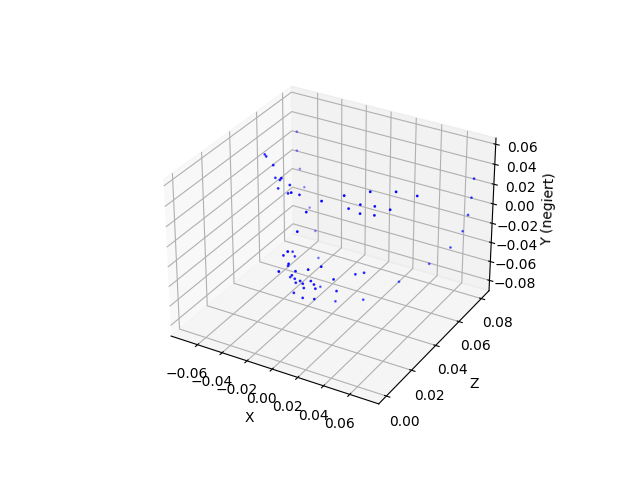
\includegraphics[width=\linewidth]{implementation/68_face_template_model.png}
        \caption{3D Gesichtsmodell bestehend aus 68 Punkten}
        \label{fig:implement:templates:dlib}
    \end{subfigure}%
    \begin{subfigure}{0.5\textwidth}
        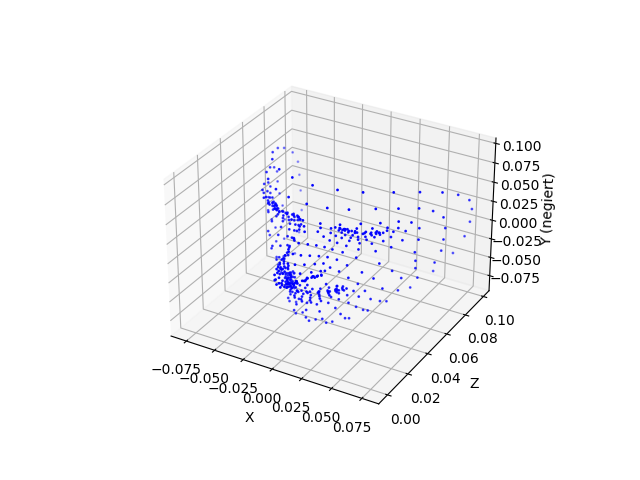
\includegraphics[width=\linewidth]{implementation/468_face_template_model.png}
        \caption{3D Gesichtsmodell bestehend aus 468 Punkten}
        \label{fig:implement:templates:mediapipe}
    \end{subfigure}
    \caption{Verwendete dreidimensionale Modelle des Kopfes mit 68 Punkten (Abbildung \ref{fig:implement:templates:dlib}) und 468 Punkten (Abbildung \ref{fig:implement:templates:mediapipe}). Zur Darstellung wurde jeweils die y-Achse invertiert.}
    \label{fig:implementation:templates}
\end{figure}

Zur Bestimmung der dreidimensionalen Position der Punkte bietet OpenCV die \textit{solvePnP} Funktion\footnote{\url{https://docs.opencv.org/4.x/d5/d1f/calib3d_solvePnP.html} (Abgerufen am 25.09.2023)} an. Mit dieser können mittels der intrinsischen Parameter der Kamera, der Liste der erkannten zweidimensionalen Gesichtspunkte und der Liste der dreidimensionalen Punkte des Modells ein Rotationsvektor $\rotationvector$ und ein Translationsvektor $\translationvector$ berechnet werden. Diese geben an, wie das dreidimensionale Modell des Kopfes gedreht und verschoben werden muss, um der dargestellten zweidimensionalen Pose zu entsprechen.

Das dreidimensionale Koordinatensystem kann dabei wie folgt beschrieben werden:

\begin{itemize}
    \item Die Kamera befindet sich im Koordinatenursprung.
    \item Die x-Achse zeigt relativ zur Kamera nach rechts und gibt die relative Position in der Breite des Bildes an.
    \item Die y-Achse zeigt relativ zur Kamera nach unten und gibt die relative Position in der Höhe des Bildes an. 
    \item Die z-Achse zeigt relativ zur Kamera nach vorn und gibt die Tiefe des Bildpunktes zur Kamera an.
\end{itemize}

Bevor das Problem gelöst werden kann, müssen die intrinischen Parameter der Kamera bestimmt werden. Dazu gehören eine Kameramatrix $\cameramatrix$ und die Verzerrungskoeffizienten der Smartphone-Kamera, mit der das Video aufgenommen wurde. Um diese exakt zu bestimmen, muss die Kamera kalibriert werden. OpenCV bietet hierfür die Funktion \textit{calibrateCamera}\footnote{\url{https://docs.opencv.org/3.4/dc/dbb/tutorial_py_calibration.html} (Abgerufen am 20.11.2023)}, mit der diese Parameter bestimmt werden können. Dazu ist jedoch ein spezieller Kalibrierungsprozess erforderlich, bei dem zum Beispiel Bilder von einem Schachbrett mit einem bestimmten Abstand der Kamera zu diesem Schachbrett aufgenommen werden. Da dieser Kalibrierungsprozess für jede Kamera durchgeführt werden müsste, ist er ungeeignet für den Anwendungsfall der PrioBike-App. Daher wurden diese Parameter geschätzt. Es ist zu beachten, dass dies zu ungenaueren Ergebnissen führt, als wenn diese Parameter exakt bestimmt würden. Zunächst wird für jedes aufgenommene Video eine Kameramatrix $\cameramatrix$ erstellt. Dazu wird die Brennweite entlang der Bildbreite sowie der Bildlänge als Bildgröße in Pixeln angenommen. Das optische Zentrum des Bildes wird in der Bildmitte angenommen.

\[
c_w = \frac{\widthvideo}{2} \qquad
c_h = \frac{\heightvideo}{2} \qquad  
\cameramatrix = \begin{pmatrix}
\widthvideo & 0 & c_w \\
0 & \heightvideo & c_h \\
0 & 0 & 1\\
\end{pmatrix}
\]

Das Bild einer Kamera kann durch radiale und tangentiale Verzerrungen beeinflusst werden. Die radiale Verzerrung bewirkt, dass eine gerade Linie in einem Bild gekrümmt wird. Die tangentiale Verzerrung führt dazu, dass Teile des Bilder näher an der Kamera erscheinen, als sie eigentlich sind. Diese Verzerrung des Bildes kann angegeben werden mittels der Verzerrungskoeffizienten $k_1$, $k_2$, und $k_3$, welche die radiale Verzerrung beschreiben, sowie mit $p_1$ und $p_2$, welche die tangentiale Verzerrung beschreiben \footnote{Siehe \url{https://docs.opencv.org/4.x/dc/dbb/tutorial_py_calibration.html} (Abgerufen am 02.11.2023)}. Kennt man diese Koeffizienten, kann man die Verzerrung des Bildes korrigieren. Im Anwendungsfall der PrioBike-App ist jedoch nicht mit größeren Verzerrungen der Bilder durch die Innenkamera des Smartphones zu rechnen. Daher werden diese Koeffizienten als 0 angenommen.

\[
\text{Verzerrungskoeffizienten} = (k_1, k_2, p_1, p_2, k_3) = (0, 0, 0, 0, 0)
\]

Nachdem diese Parameter geschätzt wurden, kann die Funktion ausgeführt werden.
Wie bereits erwähnt, liefert die Funktion als Ergebnis einen Rotationsvektor $\rotationvector$ und einen Translationsvektor $\translationvector$. Aus $\rotationvector$ wird im nächsten Schritt eine Rotationsmatrix $\rotationmatrix$ berechnet:

\[
\rotationvector = \begin{pmatrix}
    r_x \\ r_y \\ r_z
\end{pmatrix} \\
\]

\[
\theta = \|\vec{r}\| \qquad
\omega =  1- \cos \theta \qquad
\alpha = \frac{r_x}{\theta} \qquad
\beta = \frac{r_y}{\theta} \qquad
\gamma = \frac{r_z}{\theta}
\]

\[
\rotationmatrix = \begin{pmatrix}
    \alpha^2\cdot\omega + \cos \theta & \alpha\cdot\beta\cdot\omega - \gamma \cdot\sin\theta & \alpha\cdot\gamma\cdot\omega + \beta\cdot\sin\theta \\
    \alpha\cdot\beta\cdot\omega + \gamma \cdot \sin \theta & \beta^2 \cdot\omega+\cos\theta & \beta\cdot\gamma\cdot\omega-\alpha\cdot\theta \\
    \alpha\cdot\gamma\cdot\omega - \beta \cdot \sin\theta & \beta\cdot\gamma\cdot\omega + \alpha\cdot\sin\theta & \gamma^2\cdot\omega+\cos\theta \\
\end{pmatrix}
\]

Mittels der bestimmten Rotationsmatrix $\rotationmatrix$ und dem Translationsvektor $\translationvector$  können die Punkte des Kopfmodells $F_i$ (wobei $i$ der Index des entsprechenden zweidimensionalen Gesichtspunkt $\landmark$ ist) nun so rotiert und verschoben werden, dass sie der dreidimensionalen Position des dargestellten Gesichts entsprechen. Somit erhält man die dreidimensionale Position bestehend aus $\landmarkxmodel$, $\landmarkymodel$, $\landmarkzmodel$ für jeden Gesichtspunkt $L_i$.

\[
\begin{pmatrix}
   \landmarkxmodel \\ \landmarkymodel \\ \landmarkzmodel \\ 
\end{pmatrix} = F_i \cdot \rotationmatrix^T + \translationvector
\]

Anhand der dreidimensionalen Position der Gesichtspunkte kann nun das Zentrum des Kopfes $\centerface$ im dreidimensionalen Raum berechnet werden. Dieser wird definiert als das Zentrum der äußersten Punkte der Augen sowie den äußersten Punkte der Nase. Die dafür verwendeten Gesichtspunkte sind in der Tabelle  \ref{tab:implementation:used:landmarks} zu sehen.
Aus diesem Punkt $\centerface$ kann nun der Abstand des Kopfes zur Kamera im Koordinatenursprung, im folgenden $\distancefacecamera$ genannt, berechnet werden. Die Distanz $\distancefacecamera$ entspricht der Länge des Vektors vom Koordinatenursprung zu Punkt $\centerface$.

\subsection{Persistenz der Ergebnisse}

Die Ergebnisse der Gesichtserkennung eines Videos werden für jedes verwendete Gesichtsmodell in einer separaten Datei gespeichert. Die Datei ist folgendermaßen aufgebaut: In der ersten Zeile steht ein Wahrheitswert, der angibt, ob die Gesichtserkennung für das entsprechende Video vollständig abgeschlossen wurde oder nicht. Anschließend wird für jedes ausgewählte Frame $f$, in dem ein Gesicht erkannt werden konnte, ein Eintrag in die Datei eingefügt. Zu einem Eintrag gehören:

\begin{itemize}
    \item Nummer des Frames $f$ ($n$)
    \item Zeitpunkt des Frames $f$ in Millisekunden ($t$)
    \item Distanz $\distancefacecamera$
    \item Rotationsvektor $\vec{r}$
    \item Kopfzentrum $C$
    \item Translationsvektor $\translationvector$ 
    \item $EAR$
    \item Auflistung erkannter Gesichtspunkte $\landmark$
    \begin{itemize}
        \item Index $\indexlandmark$
        \item $\landmarkxmodel$
        \item $\landmarkymodel$
        \item $\landmarkzmodel$
        \item $\landmarkxnorm$
        \item $\landmarkynorm$
        \item $\landmarkznorm$
        \item $\landmarkxbild$
        \item $\landmarkybild$
    \end{itemize}
\end{itemize}

Die einzelnen Einträge sind durch eine Leerzeile getrennt. Wenn für ein Bild kein Gesicht erkannt wurde, wird in der Datei kein Eintrag erstellt. Ein Beispiel für eine solche Datei ist in Abbildung \ref{code:implementation:face:output} dargestellt.

\begin{figure}
    \centering
   \begin{lstlisting}[language=Java]
true // Video wurde vollstaendig verarbeitet

0 // Nummer des Frames 
0 // Zeitpuntk des Frames
0.2617788121569677 // Distanz zwischen Gesicht und Kamera
-0.04532,-0.01643,0.08828 // Rotationsvektor des Gesichts
-0.01548,-0.02905,0.2597 // Kopfzentrum
-0.0165,-0.0125,0.22876 // Translationsvektor des Gesichts
0.4318541506079564 // EAR
0,-0.08664,-0.04335,0.31008,0.2056,0.4109,1,222,789 // Gesichtspunkt mit Index 0
1,-0.08752,-0.02475,0.30845,0.2046,0.4464,1,221,857 // Gesichtspunkt mit Index 1
... // Face Landmarks mit Index 2 bis 66
67,-0.0278,0.02461,0.24632,0.3944,0.5521,1,426,1060 // Gesichtspunkt mit Index 67

3
99
0.2608503005208114
-0.04663,-0.00485,0.08932
-0.01503,-0.02871,0.25883
-0.01642,-0.01222,0.22787
0.5655616094861263
0,-0.0856,-0.04296,0.31005,0.2074,0.4156,1,224,798
1,-0.08651,-0.02437,0.3084,0.2056,0.4495,1,222,863
...
\end{lstlisting}
    \caption{Ausschnitt aus der Ergebnisdatei der Gesichtserkennung mit \dlib.}
    \label{code:implementation:face:output}
\end{figure}

\section{Blickrichtungsbestimmung}\label{sec:implementation:gaze}

Nachdem die Gesichtserkennung durchgeführt wurde, wird aufbauend auf den Ergebnissen der Gesichtserkennung die Blickrichtungsbestimmung durchgeführt. Hierfür wurden zwei unterschiedliche Konzepte erarbeitet. Zum einen soll die Blickrichtung mithilfe von Convolutional Neural Networks aus dem Gesicht des Radfahrers bestimmt werden, wie in Kapitel \ref{sec:concept:3d} erläutert wird. Das zweite Konzept verwendet die bei der Gesichtserkennung ermittelte Kopfdrehung als Blickrichtung, wie in Kapitel \ref{sec:concept:head} beschrieben wird. Die Implementierung der beiden Methoden zur Bestimmung der Blickrichtung und die Interpretation der Ergebnisse werden im Folgenden vorgestellt.

\subsection{Blickrichtungsbestimmung mit Convolutional Neural Networks}\label{sec:implementation:gaze:vector:models}

Im Folgenden wird die Blickrichtungsbestimmung mittels Convolutional Neural Networks beschrieben. Dazu wird zunächst die Implementierung der Modelle erläutert. Anschließend wird die Implementierung des von Cheng et al. vorgestellten Verfahrens zur Bildnormalisierung \cite{paper:basics:survey} beschrieben. Abschließend wird gezeigt, wie die Ergebnisse der Convolutional Neural Networks verwendet werden können, um einen dreidimensionalen Blickrichtungsvektor $\gazevector$ zu bestimmen.


\subsubsection{Implementierung der Convolutional Neural Networks}

Wie in Kapitel \ref{sec:concept:3d} beschrieben, wurden die Datensätze \textit{ETH-XGaze} \cite{paper:eth-xgaze}, \textit{Gaze360} \cite{paper:gaze360} und \textit{MPIIFaceGaze} \cite{paper:mpiifacegaze} ausgewählt, die als Grundlage für je ein \cnn dienen sollen. Für die generelle Implementierung der Modelle wird die \textit{PyTorch} Python Bibliothek\footnote{\url{https://pytorch.org/} (Abgerufen am 29.11.2023)} verwendet.

Für die Datensätze \ethg und \mpii stellt die \textit{pt-gaze}\footnote{\url{https://pypi.org/project/ptgaze/} (Abgerufen am 02.12.2023), \url{https://github.com/hysts/pytorch_mpiigaze_demo/tree/master} (Abgerufen am 02.12.2023)} Python Bibliothek jeweils eine Implementierung eines Convolutional Neural Networks zur Verfügung, die in dieser Arbeit verwendet werden. 

Die Implementierung des Modells, das den \ethg Datensatz verwendet, wird mit der \textit{PyTorch Image Models}\footnote{\url{https://pypi.org/project/timm/} (Abgerufen am 02.12.2023)} Python Bibliothek realisiert und beruht auf einer ResNet-18 Architektur. Zusätzlich werden die vortrainierten Gewichtungen des Modells\footnote{\url{https://github.com/hysts/pytorch_mpiigaze_demo/releases/download/v0.2.2/eth-xgaze_resnet18.pth} (Abgerufen am 25.08.2023)} durch die \textit{pt-gaze} Bibliothek bereitgestellt. 

Die Implementierung des Modells, das auf dem \mpii Datensatz beruht, kann in der \textit{pt-gaze} Bibliothek auf verschiedene Arten und Weisen konfiguriert werden. Im Rahmen dieser Arbeit wurde die Implementation des Modells\footnote{\url{https://github.com/hysts/pytorch_mpiigaze_demo/blob/master/ptgaze/models/mpiifacegaze/resnet_simple.py} (Abgerufen am 03.12.2023), Backbone: \url{https://github.com/hysts/pytorch_mpiigaze_demo/blob/master/ptgaze/models/mpiifacegaze/backbones/resnet_simple.py} (Abgerufen am 03.12.2023)} so angepasst, dass sie der Standardkonfiguration\footnote{\url{https://github.com/hysts/pytorch_mpiigaze_demo/blob/master/ptgaze/data/configs/mpiifacegaze.yaml} (Abgerufen am 03.12.2023)} der Bibliothek entspricht. Weiter musste eine Anpassungen an der Implementierung vorgenommen werden, da durch eine unterschiedliche Version des \textit{PyTorch torchvision} Python Packages ein Fehler aufgetreten ist. Speziell wird in der \textit{pt-gaze} Bibliothek das \textit{model\_urls} Attribut von \textit{torchvision.models.resnet} verwendet, um die vortrainierten Gewichtungen einer ResNet-18 Architektur zu laden. Dieses Attribut wird in der Version, die in dieser Arbeit genutzt wird\footnote{Version 0.15.2}, nicht mehr unterstützt. Daher wurde die entsprechende URL\footnote{Gemeint ist \url{https://download.pytorch.org/models/resnet18-f37072fd.pth} (Abgerufen am 03.12.2023)} manuell eingefügt. Auch für die Anwendung dieses Modells werden die vortrainierten Gewichtungen\footnote{\url{https://github.com/hysts/pytorch_mpiigaze_demo/releases/download/v0.1.0/mpiifacegaze_resnet_simple.pth} (Abgerufen am 25.08.2023)} der \textit{pt-gaze} Bibliothek verwendet. 

Für den \textit{Gaze360}-Datensatz wird die Implementierung von Abdelrahman et al. \textit{L2CS-net} \cite{paper:l2csnet} verwendet. Die Implementierung wurde in Kapitel \ref{sec:related:gaze:appearance:l2cs} vorgestellt und ist öffentlich zugänglich\footnote{\url{https://github.com/Ahmednull/L2CS-Net} (Abgerufen am 29.11.2023) verwendet. Die Implementierung des von Abdelrahman et al. vorgestellten Convolutional Neural Networks ist unter folgender URL zu finden: \url{https://github.com/Ahmednull/L2CS-Net/blob/main/l2cs/model.py} (Abgerufen am 29.11.2023)}. Auch Abdelrahman et al. stellen vortrainierte Gewichtungen\footnote{\url{https://drive.google.com/uc?id=18S956r4jnHtSeT8z8t3z8AoJZjVnNqPJ&export=download} (Abgerufen am 25.08.2023)} zur Verfügung, die in dieser Arbeit verwendet werden. Es ist jedoch aufgefallen, dass in der Implementierung von Abdelrahman et al. die Bedeutung der Pitch- und Yaw-Winkel\footnote{Siehe \url{https://github.com/Ahmednull/L2CS-Net/blob/a4d8f7fa5436a2b2b9f088471623b552a85811bd/l2cs/vis.py#L13C5-L14C39} (Abgerufen am 03.12.2023)} von der Definition in Kapitel \ref{sec:basics:eye} abweicht. Die entsprechenden Ergebnisse des Modells werden daher im Rahmen dieser Arbeit vertauscht.

Im Folgenden werden die Convolutional Neural Networks nach dem Datensatz benannt, mit dem sie trainiert wurden.

\subsubsection{Normalisierung}

Bevor die erkannten Gesichter der Radfahrenden mit den Convolutional Neural Networks verarbeitet werden können, müssen sie (wie in Kapitel \ref{sec:concept:3d}) beschrieben normalisiert werden. Dazu muss eine Projektionsmatrix $\projectionmatrix$ bestimmt werden. Für die Berechnung dieser Matrix werden folgende Daten benötigt:

\begin{itemize}
    \item die Rotationsmatrix $\rotationmatrix$, die aus dem bei der Gesichtserkennung gespeicherten Rotationsvektor $\rotationvector$ berechnet werden kann,
    \item ein Referenzpunkt im Gesicht der abgebildeten Person, um den die Kamera entlang der Längsachse gedreht wird (Zentrum des Kopfes $\centerface$),
    \item der Vektor $\vec{c}$, der vom Koordinatenursprung (Kamera) zum Zentrum des Kopfes $\centerface$ zeigt,
    \item die geschätzte Kameramatrix $\cameramatrix$ der Innenkamera des Smartphones,
    \item eine normalisierte Distanz $\hat{d}$, die den Abstand der virtuellen Kamera zum dargestellten Gesicht beschreibt,
    \item eine Skalierungsmatrix $\scalematrix$ zur Berechnung des virtuellen Abstands der Kamera zum Gesicht,
    \item die Größe des normalisierten Bildes in Pixeln,
    \item eine normalisierte Kameramatrix $\normcameramatrix$, die die virtuelle Kamera nach der Normalisierung beschreibt.
\end{itemize}

Die verwendeten normalisierten Kameramatrizen $\normcameramatrix$, Distanzen $\hat{d}$ und Bildgrößen für die Eingabebilder der einzelnen Modelle sind in Tabelle \ref{tab:implementation:gaze:camera:configs} aufgeführt.

\begin{table}[]
    \centering
    \begin{tabular}{l c c c}
    \toprule
        \textbf{Modell} & \makecell{\textbf{Normalisierte}\\ \textbf{Kameramatrix $\normcameramatrix$}}  & \textbf{Bildgröße} & \makecell{\textbf{Normalisierte}\\ \textbf{Distanz $\hat{d}$}}  \\ 
        \midrule
        ETH-XGaze\footnote{Die verwendete normalisierte Kameramatrix und Distanz stammen aus der \textit{pt-gaze} Bibliothek. Die Parameter sind unter folgender URL zu finden: \url{https://github.com/hysts/pytorch_mpiigaze_demo/blob/master/ptgaze/data/normalized_camera_params/eth-xgaze.yaml} (Abgerufen am 29.11.2023)} & $\begin{pmatrix}960 & 0 & 112 \\0 & 960 & 112 \\ 0 & 0 & 1 \end{pmatrix}$ & $224 \times 224$ & 0,6 \\
        MPIIFaceGaze\footnote{Die verwendete normalisierte Kameramatrix und Distanz stammen aus der \textit{pt-gaze} Bibliothek. Die Parameter sind unter folgender URL zu finden: \url{https://github.com/hysts/pytorch_mpiigaze_demo/blob/master/ptgaze/data/normalized_camera_params/mpiifacegaze.yaml} (Abgerufen am 29.11.2023)} & $\begin{pmatrix}1600 & 0 & 112 \\0 & 1600 & 112 \\ 0 & 0 & 1 \end{pmatrix}$ & $224 \times 224$ & 1\\
        Gaze360\footnote{Es werden die gleichen Parameter wie für \textit{ETH-XGaze} verwendet.} & $\begin{pmatrix}960 & 0 & 112 \\0 & 960 & 112 \\ 0 & 0 & 1 \end{pmatrix}$ & $224 \times 224$ & 0,6 \\
        \bottomrule
        
    \end{tabular}
    \caption{Darstellung der verwendeten Normalisierungsmatrizen, normalisierte Bildgröße und normalisierte Distanz $\hat{d}$, die für die einzelnen Datensätze, auf denen die Modelle basieren, verwendet wurden.}
    \label{tab:implementation:gaze:camera:configs}
\end{table}

Die Projektionsmatrix $\projectionmatrix$ kann dann wie folgt berechnet werden:

\[
\rotationmatrix = \begin{pmatrix}
    r_{11} & r_{12} & r_{13} \\
    r_{21} & r_{22} & r_{23} \\
    r_{31} & r_{32} & r_{33}
\end{pmatrix} \qquad R_x = \begin{pmatrix}
r_{11} \\
r_{21} \\
r_{31} 
\end{pmatrix} \qquad \scalematrix = \begin{pmatrix}
    1 & 0 & 0 \\
    0 & 1 & 0 \\
    0 & 0 & \frac{\hat{d}}{\distancefacecamera}
\end{pmatrix}
\]

\[
z_{\text{axis}} = \frac{\vec{c}}{\|\vec{c}\|} \qquad
y' = z_{\text{axis}} \times R_x \qquad
y_{\text{axis}} = \frac{y'}{\|y'\|} \qquad
x' = y_{\text{axis}} \times z_{\text{axis}} \qquad
x_{\text{axis}} = \frac{x'}{\|x'\|}
\]

\[
R_{\text{Normalisierung}} = \begin{pmatrix}
    x_{\text{axis},1} & x_{\text{axis},2} & x_{\text{axis},3} \\
    y_{\text{axis},1} & y_{\text{axis},2} & y_{\text{axis},3} \\
    z_{\text{axis},1} & z_{\text{axis},2} & z_{\text{axis},3}
\end{pmatrix}
\]

\[
T = \scalematrix \cdot R_{\text{Normalisierung}}
\]

\[
\projectionmatrix = \normcameramatrix \cdot T \cdot \cameramatrix^{-1}
\]

Diese Projektionsmatrix $\projectionmatrix$ kann dann für die Normalisierung des Bildes verwendet werden. Dazu wird die Funktion \textit{warpPerspective}\footnote{\url{https://docs.opencv.org/3.4/da/d54/group__imgproc__transform.html#gaf73673a7e8e18ec6963e3774e6a94b87} (Abgerufen am 29.11.2023)} von OpenCV verwendet. Mit dieser kann ein Bild mit gegebener Projektionsmatrix und normalisierter Bildgröße perspektivisch transformiert werden.

\subsubsection{Bestimmen der Blickrichtung}

Die normalisierten Bilder werden im Anschluss in die Convolutional Neural Networks geladen. Alle drei Modelle berechnen aus dem normalisierten Bild einen Pitch- und Yaw-Winkel, der die Blickrichtung der dargestellten normalisierten Person beschreibt. Diese beiden Winkel können wie folgt in den normalisierten Blickrichtungsvektor $\vec{g'}$ umgerechnet werden:

\[
 \vec{g'} = \begin{pmatrix}
     \cos(\text{pitch}) \cdot \sin(\text{yaw}) \\
    \sin(\text{pitch}) \\
     \cos(\text{pitch}) \cdot \cos(\text{yaw}) \\
 \end{pmatrix}
\]

Anhand der normalisierten Kopfrotation $R_\text{Normalisierung}$ kann der Vektor anschließend so rotiert werden, dass er der Blickrichtung der Person vor der Normalisierung entspricht:

\[
\gazevector = R_{\text{Normalisierung}} \cdot \vec{g'}
\]

\subsection{Blickrichtungsbestimmung anhand der Kopfrotation}

Für die Bestimmung der Blickrichtung anhand der Kopfdrehung einer abgebildeten Person wird die Rotationsmatrix $\rotationmatrix$ benötigt, die bei der Gesichtserkennung für die erkannten Gesichter der einzelnen Videoframes berechnet wurde. Weiterhin wird ein Vektor benötigt, der die Kopfdrehung einer Person repräsentiert, die keine Rotation entlang der Quer- oder Vertikalachse aufweist. Da die Tiefendimension die z-Achse ist und alle von der Kamera erfassten Objekte eine Tiefe größer als Null haben, kann ein Vektor $\vec{g'}$ bestimmt werden. Dieser Vektor ist orthogonal zur Ebene $\cameraplane$.

\[
\vec{g}' = \begin{pmatrix}
    0 \\ 0 \\ -1 \\
\end{pmatrix}
\]

Mit der Rotationsmatrix $\rotationmatrix$ kann dieser Vektor $\vec{g'}$ nun gedreht werden, um die tatsächliche Kopfdrehung darzustellen, die in diesem Konzept die Blickrichtung repräsentiert.

\[
\gazevector = \rotationmatrix \cdot \vec{g}'
\]

\subsection{Interpretation der Blickrichtung}\label{sec:implementation:gaze:interpretation}

Bisher wurden in diesem Kapitel bereits drei Convolutional Neural Networks sowie ein Ansatz zur Bestimmung der Blickrichtung aus der Kopfdrehung implementiert. Insgesamt kann also von vier verschiedenen Verfahren zur Blickrichtungsbestimmung gesprochen werden. Zusammen mit den beiden implementierten Methoden zur Gesichtserkennung mittels \dlib und \mediapipe ergeben sich somit insgesamt acht mögliche Kombinationen für ein Video, um einen Blickrichtungsvektor zu bestimmen.

Die weitere Verarbeitung dieser Kombinationen verläuft für alle gleich. Wie in den Kapiteln \ref{sec:concept:head} und \ref{sec:concept:3d} beschrieben, wird aus dem durch die Gesichtserkennung ermittelten Zentrum des Kopfes $\centerface$ und dem durch die Blickrichtungsbestimmung ermittelten Vektor $\gazevector$ eine Gerade $G$ definiert. Im nächsten Schritt wird mit dieser Geraden ein Schnittpunkt $\intersection$ mit der Ebene $\cameraplane$ berechnet.

\[G: \begin{pmatrix}
    x \\ y \\ z 
\end{pmatrix}= \centerface + m \cdot \gazevector\qquad \cameraplane: z = 0\qquad \intersection= \centerface + \frac{-\centerface_z}{\gazevector_z} \cdot \gazevector
\]

Da die Ebene $\cameraplane$ durch $z = 0$ beschrieben werden kann, kann zur Vereinfachung die z-Koordinate des Schnittpunktes $\intersection$ ignoriert werden, wodurch ein zweidimensionaler Punkt entsteht. 

Im nächsten Schritt sieht das Konzept die Definition einer Zone auf der Ebene $\cameraplane$ vor, die das virtuelle Display des Smartphones repräsentiert. Dazu wird zunächst angenommen, dass sich die Innenkamera eines Smartphones immer in der oberen Mitte des Displays befindet. Die genaue Position der Kamera wird dabei vernachlässigt. Ausgehend von dieser Annahme wurde eine Grundzone definiert, die durch ein Quadrat mit der Seitenlänge $\hitthresholdsize$ beschrieben werden kann. Diese Zone wird so positioniert, dass sich die Kamera im Koordinatenursprung in der Mitte der Oberkante dieses Quadrats befindet, wie in Abbildung \ref{fig:evaluation:threshold:normal} dargestellt.

Die Größe dieser Grundzone kann dann durch Änderung der Seitenlänge $\hitthresholdsize$ angepasst werden. Die Oberkante bleibt dabei statisch am Koordinatenursprung fixiert. Ein Beispiel für eine solche Modifikation ist in Abbildung \ref{fig:evaluation:threshold:size} dargestellt.

Bei ersten Tests wurde erkannt, dass wenn eine Person auf das Smartphone sieht, sie den Kopf dabei nur teilweise in Richtung des Smartphones neigt. Die Schnittpunkte $\intersection$ lagen daher immer oberhalb dieser Zone. Deshalb wurde ein weiterer Parameter $\hitthresholdposition$ eingeführt. Mit diesem lässt sich die Grundzone nach unten und oben entlang der y-Achse verschieben, wie in Abbildung \ref{fig:evaluation:threshold:position} zu sehen ist.

Anhand dieser zwei Parameter $\hitthresholdsize$ und $\hitthresholdposition$ kann somit eine quadratische Zone mit den Eckpunkten ($x_{\text{min}}$, $y_{\text{min}}$) und ($x_{\text{max}}$, $y_{\text{max}}$) definiert werden, wobei gilt:

\[
x_{\text{min}} = - \frac{\hitthresholdsize}{2} \qquad
x_{\text{max}} = \frac{\hitthresholdsize}{2} \qquad
y_{\text{min}} = -\hitthresholdposition \qquad
y_{\text{max}} = \hitthresholdsize - \hitthresholdposition
\]

Darauf aufbauend kann eine Funktion $h$ definiert werden, die für einen gegebenen Schnittpunkt $\intersection$ bestimmt, ob dieser Schnittpunkt innerhalb der Zone liegt oder nicht:

\[h(\intersection) = \begin{cases}
      true & \text{wenn} x_{\text{min}} \leq \intersection_x \leq x_{\text{max}} \text{und} y_{\text{min}} \leq \intersection_y \leq y_{\text{max}} \\
      false & \text{sonst}.
\end{cases}\]

Die idealen Werte für die Parameter $\hitthresholdsize$ und $\hitthresholdposition$ wurden während der Evaluation für jede der acht möglichen Kombinationen berechnet. Näheres dazu wird im Kapitel \ref{sec:evaluation:results:gaze:threshold} erläutert. 

\begin{figure}{}
    \begin{subfigure}{0.3\textwidth}
        
\includegraphics[width=\linewidth]{evaluation/threhsold-normal.jpg}
        \caption{Ausgangsposition und Ausgangsgröße der Zone}
        \label{fig:evaluation:threshold:normal}
    \end{subfigure}%
    \vspace{0.5cm}
    \begin{subfigure}{0.3\textwidth}
        
\includegraphics[width=\linewidth]{evaluation/threhsold-size.jpg}
        \caption{Zone mit vergrößerter Seitenlänge $\hitthresholdsize$}
        \label{fig:evaluation:threshold:size}
    \end{subfigure}
    \begin{subfigure}{0.3\textwidth}
        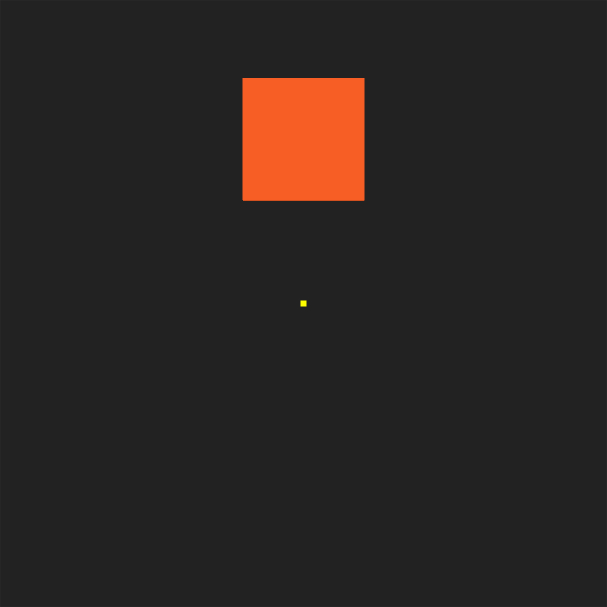
\includegraphics[width=\linewidth]{evaluation/threhsold-position.jpg}
        \caption{Zone verschoben um $\hitthresholdposition$ entlang der y-Achse}
        \label{fig:evaluation:threshold:position}
    \end{subfigure}
    \caption{Darstellung der Zone, die das Display des Smartphones beschreibt (orange dargestellt). Der gelbe Punkt zeigt den Koordinatenursprung, in dem die Kamera liegt. Für eine vereinfachte Darstellung wurde die y-Achse invertiert.}
    \label{fig:evaluation:threshold}
\end{figure}

\subsection{Persistenz der Ergebnisse}

Am Ende der Verarbeitung eines Videos wird für jede mögliche Kombination von Gesichtserkennung und Blickrichtungsbestimmung eine Datei erstellt, in der die Ergebnisse der Verarbeitung gespeichert werden. Diese Datei ist ähnlich aufgebaut wie die Datei, in der die Ergebnisse der Gesichtserkennung zwischengespeichert werden. 

In der ersten Zeile steht ein Wahrheitswert, der angibt, ob das Video vollständig verarbeitet wurde oder ob das Programm abgebrochen wurde, bevor alle Frames des Videos verarbeitet werden konnten. Anschließend folgt für jedes verarbeitete Bild ein Eintrag mit den Ergebnissen der Blickrichtungsbestimmung. Die einzelnen Einträge sind dabei durch eine Leerzeile voneinander getrennt. Zu einem Eintrag gehören:

\begin{itemize}
    \item Nummer des Frames $n$
    \item Zeitpunkt des Frames $t$ in Millisekunden
    \item Pitch-Winkel
    \item Yaw-Winkel
    \item Blickrichtungsvektor $\gazevector$ 
    \item Schnittpunkt $\intersection$
    \item $h(\intersection)$
\end{itemize}

Die Blickrichtungsbestimmung kann nur durchgeführt werden, wenn für ein Frame ein Gesicht erkannt werden konnte. Wenn kein Gesicht erkannt werden konnte, wird für dieses Frame trotzdem ein Eintrag in der Datei angelegt. Dieser besteht nur aus der Nummer des Frame $n$ und dem Zeitpunkt $t$. Ein Ausschnitt einer solchen Datei ist in Abbildung \ref{code:implementation:gaze:output} dargestellt.

\begin{figure}
    \centering
   \begin{lstlisting}[language=Java]
true // Video wurde vollstaendig verarbeitet

0 // Nummer des Frames
0 // Zeitpunkt des Frames
0.3394844 // Pitch-Winkel
0.09545608 // Yaw-Winkel
-0.159,-0.15416,-0.97517 // Blickrichtungsvektor
-0.02955,-0.14221,0.0 // Schnittpunkt mit Ebene der Kamera
false // Schnittpunkt liegt ausserhalb der definierten Zone. Person sieht nicht auf Smartphone

3 // Der Frame mit der Nummer 3 hat kein erkanntes Gesicht. Daher gibt es keine Blickrichtung
99

...
\end{lstlisting}
    \caption{Beispielhafter Ausschnitt aus einer Ergebnisdatei der Blickrichtungsbestimmung.}
    \label{code:implementation:gaze:output}
\end{figure}

\section{Zusammenfassung}

In diesem Kapitel wurde die Umsetzung der im Kapitel \ref{sec:concept} erarbeiteten Konzepte vorgestellt. Als Grundlage für die Implementierung dienten Videos von Radfahrenden. Zur Umsetzung der Konzepte wurde beschrieben, wie die einzelnen Frames eines Videos iteriert und verarbeitet werden.  Zunächst wurde dargestellt, wie die Gesichtserkennung mit \dlib \cite{paper:dlib:main} und \mediapipe \cite{paper:mediapipe} für die einzelnen Frames durchgeführt wird. Dabei werden sowohl die Bilder mit den erkannten Gesichtsmerkmalen als auch die Originalbilder gespeichert. Diese werden für die Auswertung benötigt. Außerdem wurde beschrieben, wie die Ergebnisse der Gesichtserkennung gespeichert werden. Aufbauend auf der Gesichtserkennung wurden anschließend die beiden Konzepte zur Bestimmung der Blickrichtung implementiert. Dazu wurde die Erkennung der Kopfdrehung als Blickrichtung sowie die Erkennung der Blickrichtung mit drei verschiedenen Convolutional Neural Networks umgesetzt. Damit ergeben sich insgesamt vier verschiedene Methoden, um aus einem erkannten Gesicht eine Blickrichtung zu bestimmen. Zusammen mit den beiden Methoden zur Gesichtserkennung ergeben sich somit acht verschiedene Möglichkeiten zur Bestimmung eines Blickrichtungsvektors. Anhand des ermittelten Blickrichtungsvektors und der erkannten Gesichtsmerkmale wurde anschließend beschrieben, wie die Bestimmung eines Schnittpunktes $\intersection$ mit der Ebene $\cameraplane$ implementiert wurde und wie dieser für die Entscheidung, ob Radfahrende auf ihr Smartphone schauen, interpretiert werden kann.










  \chapter{Evaluation}\label{sec:evaluation}

In diesem Kapitel wird die Evaluation der Arbeit vorgestellt. Generell soll untersucht werden, welches der vorgestellten Konzepte am besten geeignet ist, um festzustellen, wann Radfahrende auf ihr Smartphone schauen. Des Weiteren soll untersucht werden, wie gut verschiedene Umgebungsbedingungen und Störfaktoren kompensiert werden können. Dazu wird in diesem Kapitel zunächst ein Überblick über die Planung und Vorbereitung der Evaluation gegeben. Danach werden die Ergebnisse vorgestellt und diskutiert.

\section{Planung und Vorbereitung}

Mit der Evaluation sollen verschiedene Erkenntnisse gewonnen werden. Wie bereits erwähnt, liegt dabei der Fokus auf der Frage, welches Konzept am besten geeignet ist, die Blickrichtung von Radfahrenden zu ermitteln.

Um dies zu überprüfen, sollen Videos von Radfahrenden während der Fahrt mit der Innenkamera des Smartphones aufgenommen werden. Dabei sollen möglichst viele verschiedene Situationen dargestellt werden. Die Videos werden anschließend mit der Implementierung der Konzepte verarbeitet. Um einen Vergleichswert für die Ergebnisse zu schaffen, soll zunächst eine Ground Truth erstellt werden, die für jedes Bild der Videos angibt, ob die Person auf das Smartphone schaut oder nicht. Außerdem sollen Idealwerte für die im Kapitel \ref{sec:implementation:gaze:interpretation} beschriebenen Parameter ermittelt werden, mit denen ein virtuelles Smartphone modelliert werden soll. Bei der Entwicklung der Konzepte wurde die Annahme getroffen, dass wenn keine Blickrichtung ermittelt werden kann, die Person zu diesem Zeitpunkt nicht auf das Smartphone schaut, was ebenfalls während der Evaluation überprüft werden soll. 

Außerdem wird der Einfluss von geschlossenen Augen auf die Ergebnisse der Arbeit untersucht. Die Erkennung geschlossener Augen wurde im Kapitel \ref{sec:implementation:gaze:ear} beschrieben. Dafür wird der $\ear$-Wert berechnet. Um daraus erkennen zu können, ob die Augen einer Person geschlossen sind, muss bei der Auswertung ein Grenzwert $\earthreshold$ festgelegt werden. Um dies zu untersuchen, muss für die zu verarbeitenden Bilder entschieden werden, ob die Augen der abgebildeten Person geschlossen sind, um eine Ground Truth zu erstellen.

Ein wichtiger Teil der Blickrichtungsbestimmung ist die Erkennung von Gesichtern in einem Bild. Hierfür wurden zwei verschiedene Verfahren implementiert. Es soll untersucht werden, welche sich am besten für die Erkennung der Gesichter von Radfahrenden eignet und wie gut die beiden Verfahren unter verschiedenen Umgebungsbedingungen funktionieren. 

\subsection{Aufnahme von Videos}\label{sec:evaluation:videos}

Um das implementierte Konzept zu testen, wurden insgesamt 24 Videos von vier verschiedenen Personen aufgenommen. Die Personen werden im folgenden als Person A, B, C und D bezeichnet. Dabei muss angemerkt werden, dass ein Großteil der Videos \markus zeigen. Alle Teilnehmenden waren in das Ziel des Experiments eingeweiht und wussten daher, dass anhand der Aufnahme bestimmt werden soll, zu welchen Zeitpunkten sie auf das Smartphone sehen. Ihr Blickverhalten in den Videos könnte dadurch beeinflusst wurden sein. Die Videos zeigen die Probanden beim Fahrradfahren. Die einzige Ausnahme ist Video 06 von Person A. In diesem Video sitzt die Person auf einer Bank, frontal zu der Kamera und sieht dabei in alle Richtungen neben das Smartphone.

\begin{figure}[H]
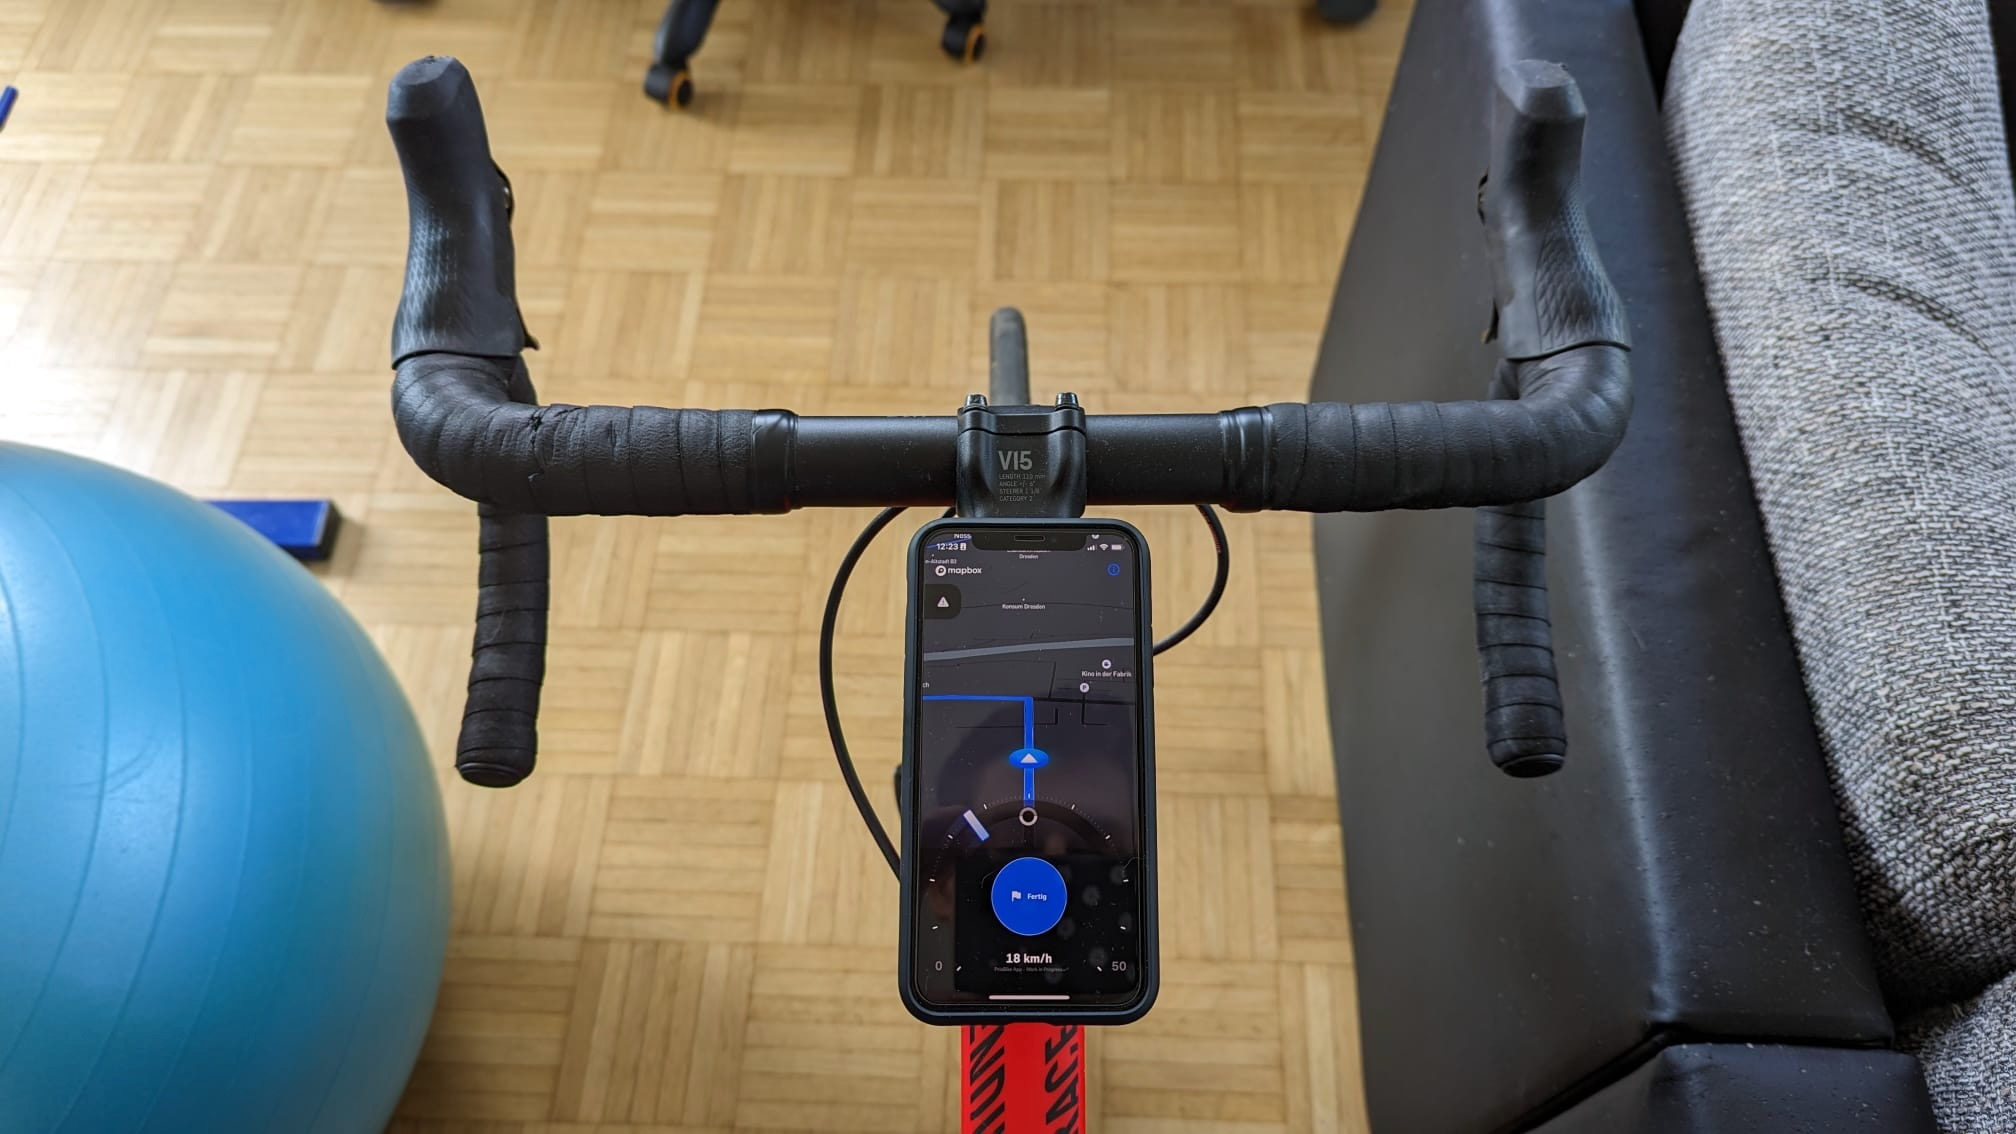
\includegraphics[width=\linewidth]{evaluation/Halterung_Philipp.jpeg}
\caption{Smartphone-Halterung von \philipp.}\label{fig:evaluation:philipp:halterung}
\end{figure}

\begin{figure}[]
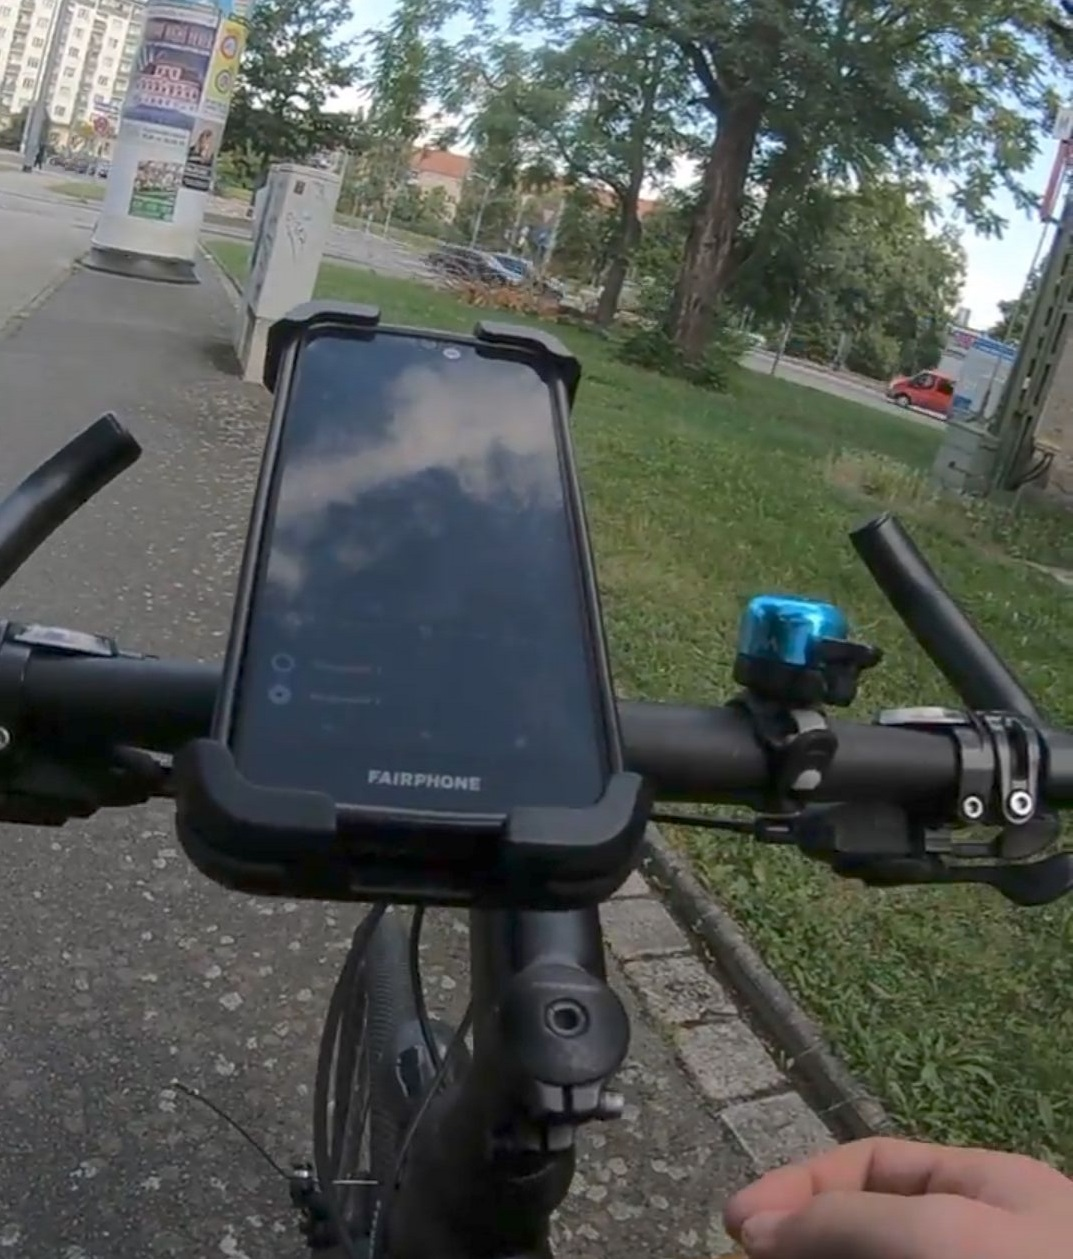
\includegraphics[width=0.5\linewidth]{evaluation/halterung.jpg}
\caption{Am Lenker befestigte Smartphone-Halterung von \florian. Person A und B verwenden eine ähnliche Halterung.}\label{fig:evaluation:default:halterung}
\end{figure}

Die Smartphones wurden mittels einer Halterung am Fahrrad befestigt. Person A, B und C verwendeten eine Halterung, welche am Lenker des Fahrrads befestigt wurde, wie sie beispielhaft in Abbildung \ref{fig:evaluation:default:halterung} zu sehen ist. Dabei wurde versucht, eine Reichweite von Blickwinkeln der Innenkamera des Smartphones auf die Person zu erzeugen, indem die Halterungen an anderen Stellen des Lenkers befestigt wurden. Person D verwendet eine Halterung, wodurch ein generell anderer Winkel auf die Person gegeben ist. Die Halterung ist in Abbildung \ref{fig:evaluation:philipp:halterung} zu sehen. Die Probanden haben für die Aufnahme der Videos unterschiedliche Geräte verwendet. Eine Übersicht über die verwendeten Geräte ist in Tabelle \ref{tab:evaluation:devices} zu sehen.

\begin{table}[]
\begin{tabular}{c l}
\toprule
\textbf{Person} & \textbf{Gerät} \\ \midrule
A      & Samsung Galaxy S10 \\
B      & Google Pixel 5     \\
C      & Fairphone 3+       \\
D      & iPhone XS     \\ \bottomrule    
\end{tabular}
\caption{Übersicht über die verwendeten Smartphones.}
\label{tab:evaluation:devices}
\end{table}

Es gab keine Vorgaben, wie sich die Personen auf dem Fahrrad verhalten sollten. Die Videos wurden jedoch mit dem Ziel aufgenommen, möglichst viele verschiedene Situationen darzustellen. So wurde darauf geachtet, dass möglichst viele verschiedene Wettersituationen, wie sonniges oder bewölktes Wetter, dargestellt werden. Es wurden auch Videos bei Nacht aufgenommen. Außerdem soll die Auswirkungen von Brillen untersucht werden. Daher gibt es Videos, in denen die Personen eine Brille oder Sonnenbrille tragen, sowie Videos, in denen keine Brille getragen wird. Zusätzlich ist zu beachten, dass in manchen Videos ein Verhalten simuliert wurde, das in realen Situationen wahrscheinlich nicht so auftreten würde. So neigt zum Beispiel \philipp in Video 10 den Kopf besonders stark zum Smartphone-Display, wenn die Person auf das Smartphone schaut.

Alle Videos wurden im MP4-Format gespeichert\footnote{Die Videos von \philipp (Video 9 und 10) wurden im MOV-Format gespeichert und vor der Verarbeitung des Videos in das MP4-Format konvertiert.}. Die Videos wurden im Hochformat mit einem Seitenverhältnis von 9:16 und mit einer Bildrate von 30 Bildern pro Sekunde aufgenommen\footnote{Das Video von Person C (Video 8) wurde mit 60 Bildern pro Sekunde aufgenommen und anschließend auf 30 Bilder pro Sekunde komprimiert.}. Die Videos haben eine Auflösung von $1080 \times 1920$ Pixel. Bei der Zerlegung der Videos in die einzelnen Frames ergeben sich insgesamt 67.017 Bilder. Wie in Kapitel \ref{sec:implemenation:video} erwähnt, wird davon nur jedes dritte Bild für die Evaluation verarbeitet. Insgesamt werden also 22.339 Frames in der Auswertung berücksichtigt. Eine Übersicht über die aufgenommen Videos ist in den Tabellen \ref{tab:evaluation:videos:1} und \ref{tab:evaluation:videos:2} dargestellt.

\begin{table}[]
\begin{tabular}{c c r p{2cm} p{4cm} c c}
\toprule
\textbf{Video} & \textbf{Person} & \textbf{Frames}  & \textbf{Datum} & \textbf{Besonderheiten} & \textbf{Wetter} & \textbf{Accessoire}     \\ \midrule
01   & A  & 1.427     & 26.08.2023, 17:22 Uhr &  & \Cloud & \tikz{\duck[invisible,squareglasses]}                       \\
02   & A  & 1.267     & 26.08.2023, 17:27 Uhr &  & \Cloud  & \tikz{\duck[invisible,squareglasses]}                     \\
03   & A  & 1.238     & 26.08.2023, 17:31 Uhr & & \Cloud & \tikz{\duck[invisible,squareglasses]}                      \\
04   & A  & 1.573     & 26.08.2023, 17:42 Uhr & Holpriger Untergrund & \Cloud & \tikz{\duck[invisible,squareglasses]} \\
05   & A  & 1.427     & 26.08.2023, 17:48 Uhr & Holpriger Untergrund & \Cloud & \tikz{\duck[invisible,squareglasses]} \\
06   & A  & 674       & 04.09.2023, 14:22 Uhr & Person in Ruhe, sitzend auf Bank  & \Sun\footnote{Person A befindet sich in einem ausgeleuchteten Raum.} &  \tikz{\duck[invisible,squareglasses]}                    \\
07   & B  & 2.623     & 05.09.2023, 13:53 Uhr &  & \Sun &  \tikz{\duck[invisible,sunglasses]}  \\
08   & C  & 3.596     & 05.09.2023, 17:22 Uhr & Helm & \Sun & \\
09   & D  & 4.922     & 05.09.2023, 17:42 Uhr & Helm, Halterungsposition & \Sun & \\
10  & D  & 3.268     & 05.09.2023, 17:46 Uhr & Helm, Halterungsposition, Versucht mit Kopfrotation auf Gerät zu schauen & \Sun & \tikz{\duck[invisible,sunglasses]} \\
11  & A  & 7.098     & 06.09.2023, 11:32 Uhr &  & \Sun & \tikz{\duck[invisible,squareglasses]}\footnote{Person A nimmt die Brille während der Fahrt ab.}  \\
12  & A  & 4.684     & 06.09.2023, 11:36 Uhr & Holpriger Untergrund & \Sun & \tikz{\duck[invisible,squareglasses]}   \\
13  & A  & 9.172     & 06.09.2023, 11:41 Uhr & Holpriger Untergrund & \Sun & \tikz{\duck[invisible,squareglasses]} \\
14  & A  & 3.744     & 06.09.2023, 11:46 Uhr & sehr sonnig & \Sun & \tikz{\duck[invisible,squareglasses]}\\
15  & A  & 2.334     & 06.09.2023, 11:48 Uhr & sehr sonnig& \Sun & \\
16  & A  & 785       & 06.09.2023, 11:51 Uhr &  & \Sun & \tikz{\duck[invisible,squareglasses]}\\
17  & A  & 2.448     & 06.09.2023, 11:57 Uhr & Halterungsposition & \Sun &  \\
18  & A  & 2.525     & 08.09.2023, 09:32 Uhr &  & \Sun & \\
19  & A  & 1.568     & 08.09.2023, 10:01 Uhr &  & \Sun &  \\
\bottomrule
\end{tabular}
\caption{Teil 1 der Übersicht über die aufgenommenen Videos. Die Übersicht zeigt die dargestellte Person, die Anzahl der Bilder des Videos, den Aufnahmezeitpunkt sowie Besonderheiten, die in diesem Video zu sehen sind. Außerdem wird das Wetter angezeigt. \Cloud\xspace bedeutet bewölkter Himmel. \Sun\xspace bedeutet sonniges Wetter. \leftmoon bedeutet klarer Nachthimmel. Außerdem werden Accessoires gezeigt, die von den dargestellten Personen getragen werden. \protect\tikz{\duck[invisible,squareglasses]} bedeutet, dass die Person eine Brille trägt. \protect\tikz{\duck[invisible,sunglasses]} bedeutet, dass die Person eine Sonnenbrille trägt.}
\label{tab:evaluation:videos:1}
\end{table}

\begin{table}[]
\begin{tabular}{c c r p{2cm} p{4cm} c c}
\toprule
\textbf{Video} & \textbf{Person} & \textbf{Frames}  & \textbf{Datum} & \textbf{Besonderheiten} & \textbf{Wetter} & \textbf{Accessoire}     \\ \midrule
20  & A  & 3.250     & 08.09.2023, 13:44 Uhr &  & \Sun & \tikz{\duck[invisible,squareglasses]} \\
21  & A  & 2.315     & 08.09.2023, 13:47 Uhr &  & \Sun & \tikz{\duck[invisible,squareglasses]} \\
22  & A  & 1.893     & 10.09.2023, 20:22 Uhr & sehr dunkle Umgebung & \leftmoon & \tikz{\duck[invisible,squareglasses]}\\
23  & A  & 1.450     & 10.09.2023, 20:37 Uhr & dunkle Umgebung, vereinzelt Laternen  & \leftmoon & \tikz{\duck[invisible,squareglasses]}\\
24  & A  & 1.736     & 10.09.2023, 20:41 Uhr & dunkle Umgebung, ausgeleuchtete Hauptstraße & \leftmoon & \tikz{\duck[invisible,squareglasses]} \\
\bottomrule
\end{tabular}
\caption{Teil 2 der Übersicht über die Videos.}
\label{tab:evaluation:videos:2}
\end{table}

\subsection{Erstellung Ground Truth}\label{sec:evaluation:ground:truths}

In der Evaluation soll untersucht werden, zu welchen Zeitpunkten die Person auf das Smartphone sieht. Um dafür einen Vergleichswert zu haben, muss eine Ground Truth für die einzelnen Frames erstellt werden, die angibt, ob eine Person auf das Smartphone sieht oder nicht. Wie in Kapitel \ref{sec:implemenation:video} beschrieben, werden dafür die einzelnen Frames des Videos als Bild gespeichert. Während der Aufnahme der Videos war es nicht möglich, die Ground Truth automatisiert zu erstellen. Wie in der Arbeit von Smith et al. \cite{paper:columbia} erwähnt, können wir Menschen jedoch sehr gut erkennen, ob eine Person uns ansieht oder nicht. Die bearbeiteten Bilder der Videos sollen daher von einem Menschen annotiert werden. Die Bilder können in eine der drei folgenden Kategorien eingeordnet werden:

\begin{itemize}
\item A.0) Person sieht nicht auf das Gerät (siehe Abbildung \ref{fig:evaluation:gaze:no}).
\item A.1) Person sieht auf das Gerät (siehe Abbildung \ref{fig:evaluation:gaze:yes}).
\item A.2) Augen oder Gesicht der Person sind nicht im Bild (siehe Abbildung \ref{fig:evaluation:gaze:not_sure}).
\end{itemize}

\begin{figure}{}
    \begin{subfigure}{0.3\textwidth}
        
\includegraphics[width=\linewidth]{evaluation/sieht_nicht_0.jpg}
        \caption{Person sieht nicht auf das Smartphone.}
        \label{fig:evaluation:gaze:no}
    \end{subfigure}
    \begin{subfigure}{0.3\textwidth}
        
\includegraphics[width=\linewidth]{evaluation/sieht_nicht_1.jpg}
        \caption{Person sieht auf das Smartphone.}
        \label{fig:evaluation:gaze:yes}
    \end{subfigure}
    \begin{subfigure}{0.3\textwidth}
        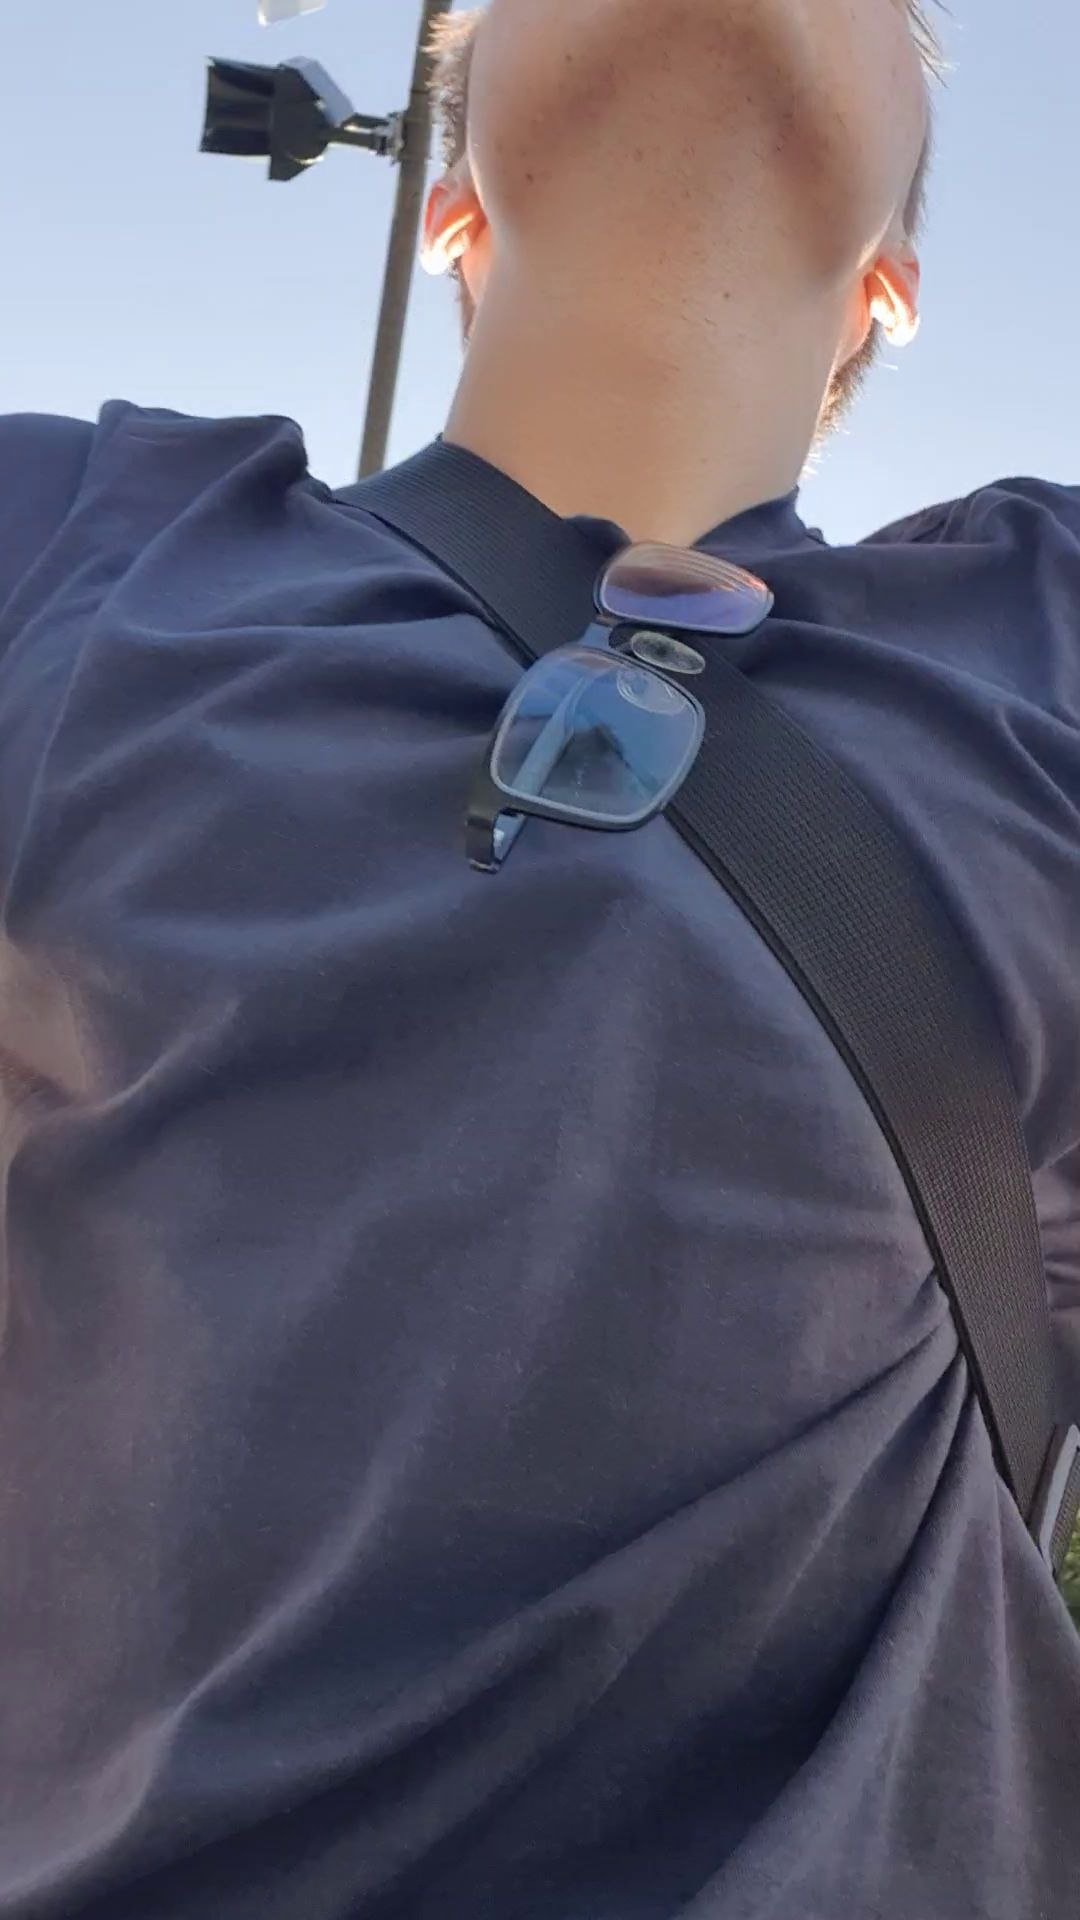
\includegraphics[width=\linewidth]{evaluation/sieht_nicht_2.jpg}
        \caption{Gesicht von Person ist außerhalb des Bildes.}
        \label{fig:evaluation:gaze:not_sure}
    \end{subfigure}
    \caption{Beispiel für die einzelnen Kategorien der Ground Truth für den Blickkontakt einer Person mit dem Display eines Smartphones.}
    \label{fig:evaluation:gaze:labels}
\end{figure}

Dabei wird angenommen, dass wenn das Gesicht der Person nicht erkennbar ist, die Person auch nicht auf das Smartphone sieht. 

Weiter soll bei der Evaluation ein Grenzwert für das \textit{Eye Aspect Ratio} ($EAR$) bestimmt werden, um geschlossene Augen erkennen zu können. Dafür muss für jedes dieser Bilder zusätzlich entschieden werden, ob die Augen der Person geschlossen sind. Jedes Bild wird dabei einer der folgenden Kategorien zugeordnet:

\begin{itemize}
    \item B.0) Augen geschlossen (siehe Abbildung \ref{fig:evaluation:eye:closed})
    \item B.1) Augen geöffnet (siehe Abbildung \ref{fig:evaluation:eye:open})
    \item B.2) Augen nicht erkenntlich (siehe Abbildung \ref{fig:evaluation:eye:not_sure})
\end{itemize}

\begin{figure}{}
    \begin{subfigure}{0.3\textwidth}
        
\includegraphics[width=\linewidth]{evaluation/auge_geschlossen.jpg}
        \caption{Augen der Person sind geschlossen.}
        \label{fig:evaluation:eye:closed}
    \end{subfigure}
    \begin{subfigure}{0.3\textwidth}
        
\includegraphics[width=\linewidth]{evaluation/auge_offen.jpg}
        \caption{Augen der Person sind geöffnet.}
        \label{fig:evaluation:eye:open}
    \end{subfigure}
    \begin{subfigure}{0.3\textwidth}
        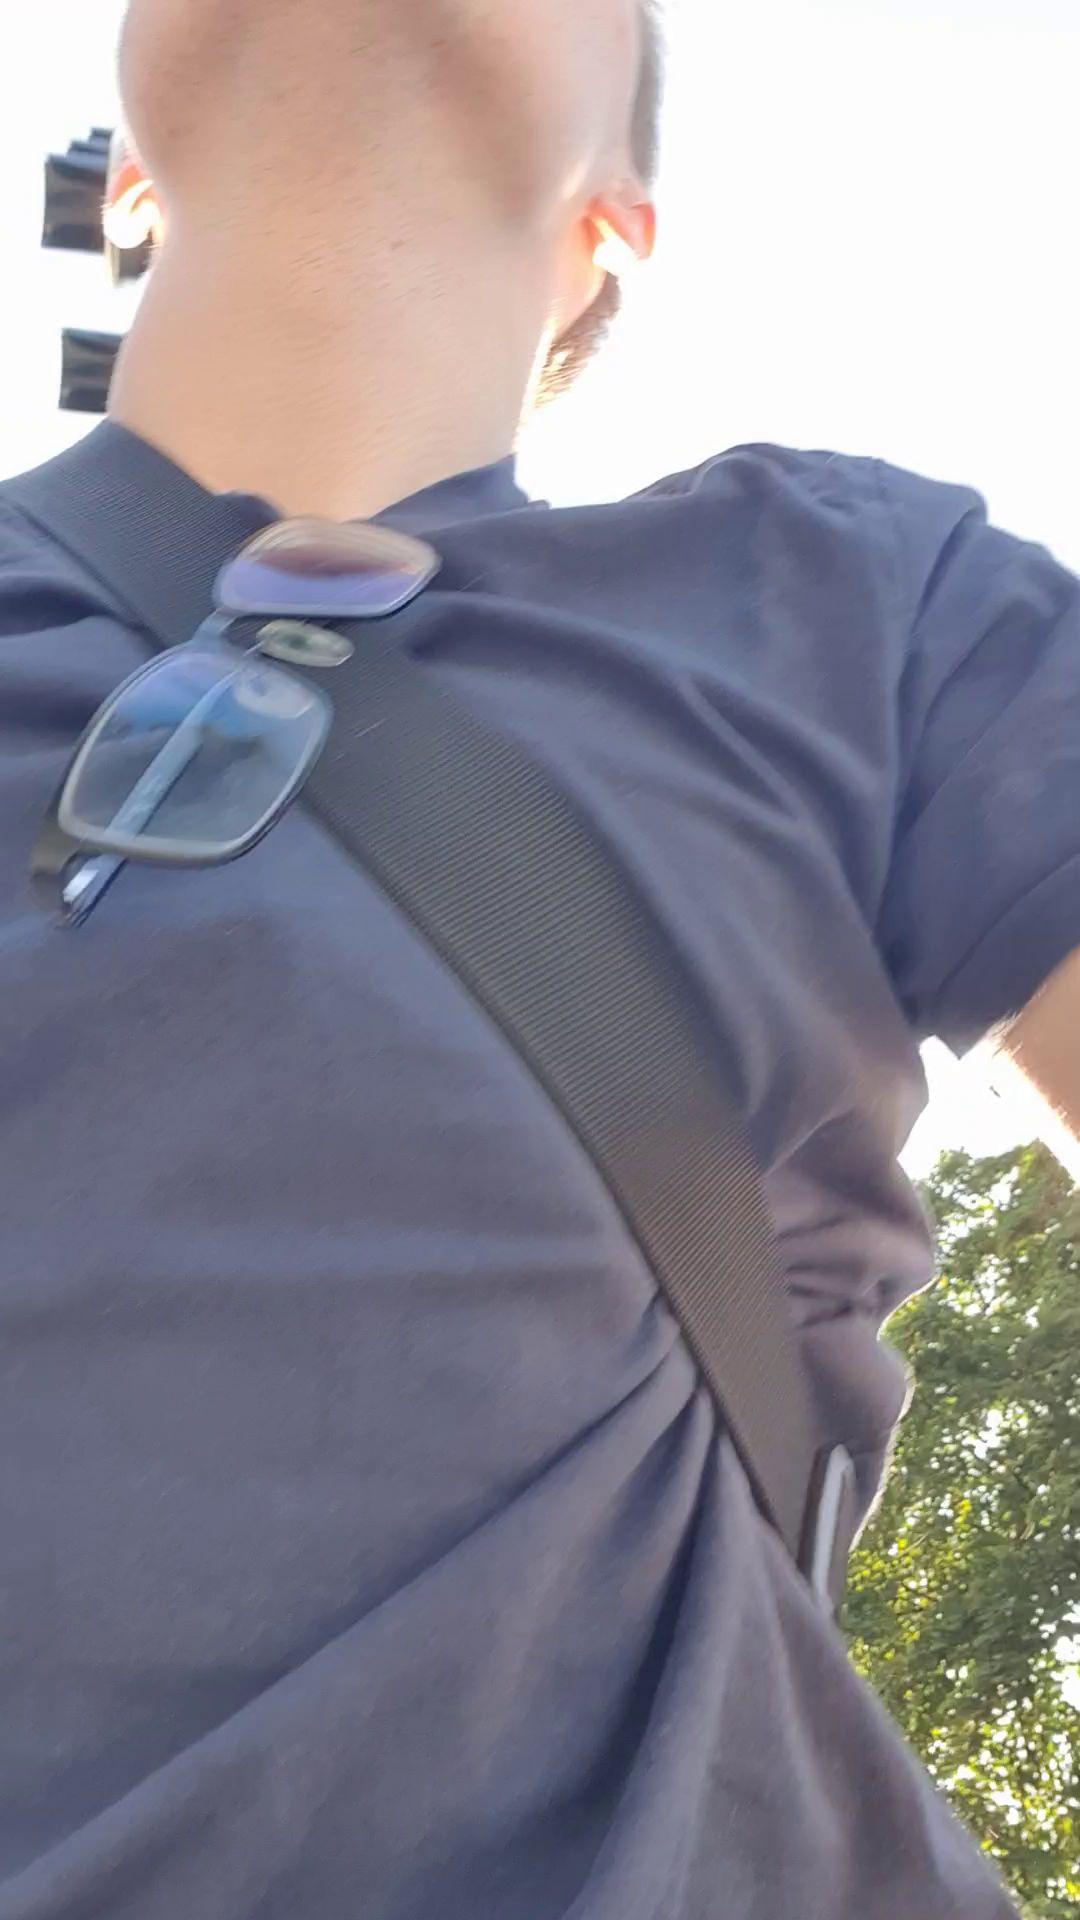
\includegraphics[width=\linewidth]{images/evaluation/auge_none.jpg}
        \caption{Augen der Person sind außerhalb des Bildes.}
        \label{fig:evaluation:eye:not_sure}
    \end{subfigure}
    \caption{Beispiel für die einzelnen Kategorien der Ground Truth für den Blickkontakt einer Person mit dem Display eines Smartphones.}
    \label{fig:evaluation:eye:labels}
\end{figure}


Für die Erstellung der Ground Truth wurde eine kleine Gruppe von Personen ausgewählt und instruiert. Diese Gruppe von Personen hat dann das Kategorisieren der Bilder durchgeführt. Um menschliche Fehler zu vermeiden, wurde der Prozess nach Abschluss des ersten Durchgangs wiederholt. Unterschiede zwischen dem ersten und dem zweiten Durchgang wurden anschließend in der Gruppe diskutiert und entschieden. 

Da sowohl die Ground Truth für den Blickkontakt als auch für die Erkennung von geschlossenen Augen aus drei Kategorien bestehen, können diese in einem gemeinsamen Dateiformat gespeichert werden. Dafür wird jeder Kategorie ein numerischer Wert zwischen 0 und 2 zugeordnet. Die genaue Zuordnung ist in Tabelle \ref{tab:evaluation:labels:numeric:values} dargestellt. Die Ergebnisse werden dann in einer Datei gespeichert. Ein Ausschnitt einer solchen Datei ist in Abbildung \ref{code:evaluation:labels:output} dargestellt. Für jeden Frame des Videos wird ein eigener Eintrag in der entsprechenden Datei erzeugt. Dieser besteht aus der Nummer des Frames $n$ und dem entsprechenden numerischen Wert der Kategorie, welche durch ein Semikolon getrennt werden. Wenn für einen Frame noch keine Kategorie festgelegt wurde, erhält dieser Frame den Wert 3. Am Anfang der Datei steht ein Wahrheitswert, der angibt, ob allen vorhandenen Bildern eine Kategorie zugewiesen wurde.

\begin{table}[]
    \centering
    \begin{tabular}{c c c}
    \toprule
         \textbf{Wert} & \makecell{\textbf{Ground Truth}\\\textbf{Blickkontakt}} & \makecell{\textbf{Ground Truth}\\\textbf{Augen geöffnet}} \\ \midrule
         0 & A.0 & B.0 \\
         1 & A.1 & B.1 \\
         2 & A.2 & B.2 \\
         \bottomrule
    \end{tabular}
    \caption{Numerischer Wert der Kategorien der beiden Ground Truths.}
    \label{tab:evaluation:labels:numeric:values}
\end{table}

\begin{figure}
    \centering
   \begin{lstlisting}[language=Java]
false // Nicht alle Frames des Videos wurden in eine Kategorie eingeordnet
0;0 // Der Frame mit der Nummer 0 gehoert zur Kategorie 0
3;1 // Der Frame mit der Nummer 3 gehoert zur Kategorie 1
6;0
9;2 // Der Frame mit der Nummer 9 gehoert zur Kategorie 2
12;3 // Fuer den Frame 12 wurde noch keine Kategorie festgelegt
15;3 
...
\end{lstlisting}
    \caption{Ausschnitt einer Datei die Ground Truth Daten enthält.}
    \label{code:evaluation:labels:output}
\end{figure}


\subsection{Qualität der Gesichtserkennung}\label{sec:evaluation:plan:quality:face}

Wie bereits in Kapitel \ref{sec:concept:head} diskutiert, muss für eine genaue Auswertung der Gesichtserkennung die mittlere Abweichung der erkannten Gesichtsmerkmale von ihrer tatsächlichen Position \cite{paper:evaluation-face} bestimmt werden. Im Rahmen dieser Arbeit würde dies bedeuten, dass für alle 22.339 verarbeiteten Bilder die tatsächliche Position einiger markanter Gesichtspunkte manuell im Bild markiert werden muss. Dies war im zeitlichen Rahmen dieser Arbeit nicht realisierbar. Daher wurde entschieden, die Gesichtserkennung qualitativ zu bewerten. Dazu wurden, wie in Kapitel \ref{sec:implementation:face:export:landmarks} beschrieben, während der Verarbeitung der Videos die Bilder der erkannten Gesichter mit den markierten Gesichtspunkten gespeichert. Zur besseren Übersicht wurden markante Punkte im Gesicht farblich hervorgehoben, um die Qualitätsbeurteilung zu erleichtern. Die Bilder mit den erkannten Gesichtern wurden dann manuell in eine der drei folgenden Kategorien eingeordnet:  

\begin{itemize}
\item Gut erkannt (siehe Abbildungen \ref{fig:evaluation:face:dlib:good} und \ref{fig:evaluation:face:mediapipe:good})
\item Ungenau erkannt (siehe Abbildungen \ref{fig:evaluation:face:dlib:medium} und \ref{fig:evaluation:face:mediapipe:medium})
\item Schlecht erkannt (siehe Abbildungen \ref{fig:evaluation:face:dlib:bad} und \ref{fig:evaluation:face:mediapipe:medium})
\end{itemize}

Indirekt kann noch eine vierte Kategorie abgeleitet werden, die Bilder beinhaltet, in denen kein Gesicht erkannt werden konnte.

Um eine einheitliche Bewertung zu gewährleisten, wurden alle erkannten Gesichter von derselben Person bewertet. 

\begin{figure}{}
    \begin{subfigure}{0.33\textwidth}
        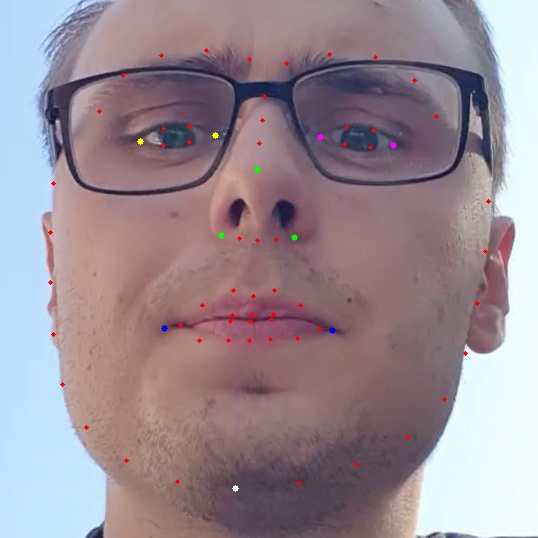
\includegraphics[width=0.9\linewidth]{evaluation/dlib_gute_erkennung.jpg}
        \caption{Gut erkannte Gesichtsmerkmale (dlib)}
        \label{fig:evaluation:face:dlib:good}
    \end{subfigure}%
    \begin{subfigure}{0.33\textwidth}
        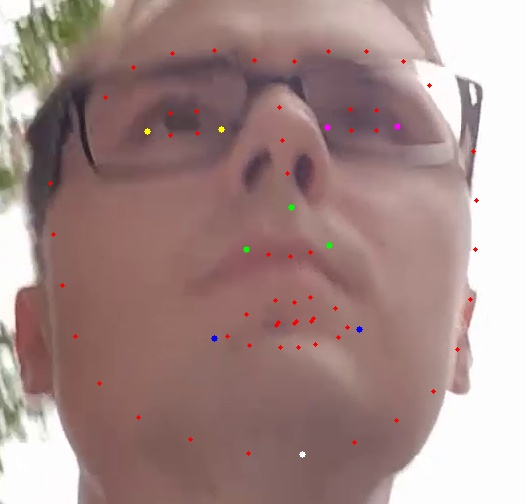
\includegraphics[width=0.9\linewidth]{evaluation/dlib_ungenaue_erkennung.jpg}
        \caption{Ungenau erkannte Gesichtsmerkmale (dlib)}
        \label{fig:evaluation:face:dlib:medium}
    \end{subfigure}
    \begin{subfigure}{0.33\textwidth}
        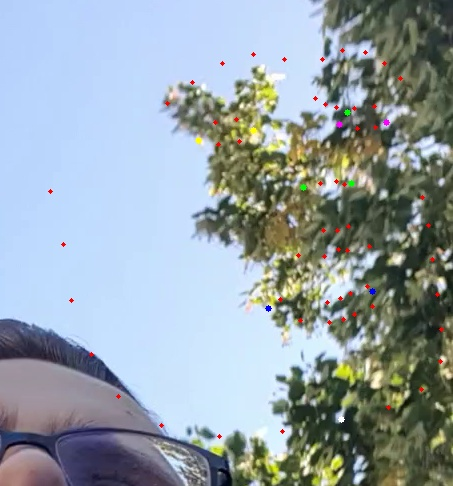
\includegraphics[width=0.9\linewidth]{evaluation/dlib_schlechte_erkennung.jpg}
        \caption{Schlecht erkannte Gesichtsmerkmale (dlib)}
        \label{fig:evaluation:face:dlib:bad}
    \end{subfigure}
    \begin{subfigure}{0.33\textwidth}
        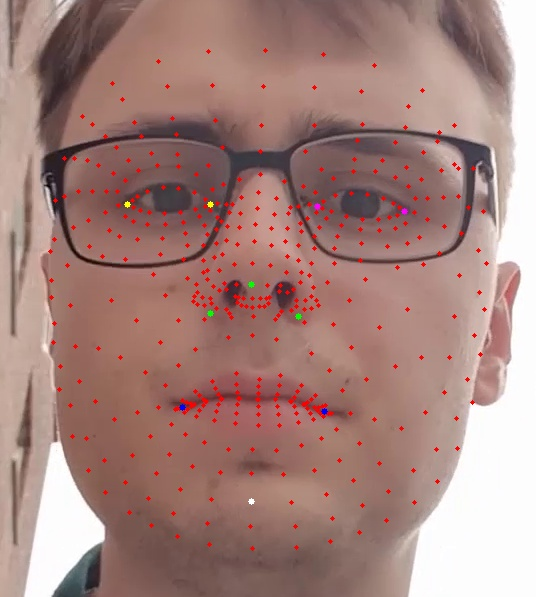
\includegraphics[width=0.9\linewidth]{evaluation/mediapipe_gute_erkennung.jpg}
        \caption{Gut erkannte Gesichtsmerkmale (MediaPipe)}
        \label{fig:evaluation:face:mediapipe:good}
    \end{subfigure}%
    \begin{subfigure}{0.33\textwidth}
        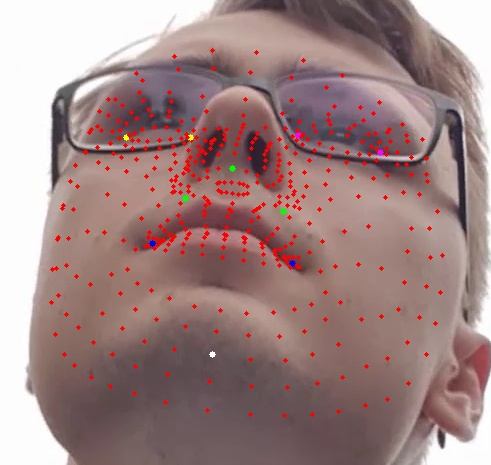
\includegraphics[width=0.9\linewidth]{evaluation/mediapipe_ungenaue_erkennung.jpg}
        \caption{Ungenau erkannte Gesichtsmerkmale (MediaPipe)}
        \label{fig:evaluation:face:mediapipe:medium}
    \end{subfigure}
    \begin{subfigure}{0.33\textwidth}
        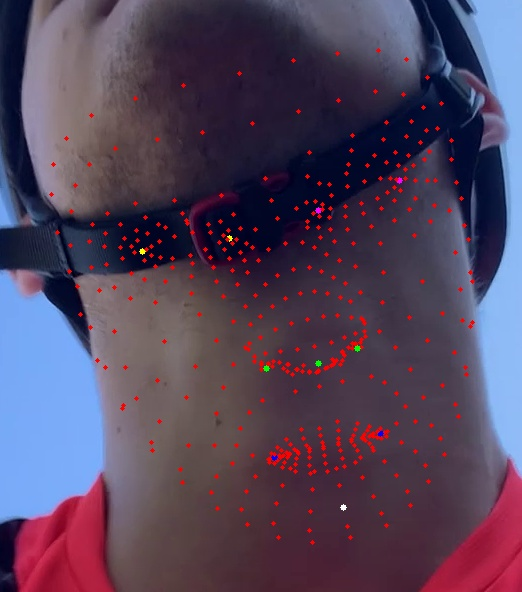
\includegraphics[width=0.9\linewidth]{evaluation/mediapipe_schlecht_erkennung.jpg}
        \caption{Schlecht erkannte Gesichtsmerkmale (MediaPipe)}
        \label{fig:evaluation:face:mediapipe:bad}
    \end{subfigure}
    \caption{Beispiele für verschiedene Qualitäten der erkannte Gesichter von \dlib und \mediapipe.}
    \label{fig:evaluation:face}
\end{figure}

\subsection{Webanwendung für die Evaluation}\label{sec:evaluation:plan:tool}

Für die Evaluation wurde eine Webanwendung mit Angular\footnote{\url{https://angular.io/} (Abgerufen am 31.10.2023)} entwickelt. Sie besteht aus zwei Ansichten. Zum einen gibt es eine Ansicht, die für die Erstellung der Ground Truth entwickelt wurde. Zum anderen gibt es eine Ansicht, mit der die Ergebnisse der Gesichtserkennung und der Blickrichtungsbestimmung visualisiert werden können, um so mögliche Fehlerquellen zu identifizieren und zu verstehen. Beide Ansichten werden im Folgenden näher vorgestellt.

\subsubsection{Ansicht Ground Truth}

Für die effiziente Erstellung der Ground Truth sowohl für Blickkontakt als auch für geschlossene Augen wurde eine Ansicht erstellt. Ein Beispiel für diese Ansicht ist in Abbildung \ref{fig:evaluation:tool} dargestellt. In der Mitte der Ansicht ist das aktuelle Bild zu sehen. Links und rechts davon befinden sich zwei große Schaltflächen. Der linke rote Button speichert je nach aktueller Auswahl die Kategorie A.0 oder B.0 für das angezeigte Bild. Der rechte grüne Knopf wird für die Kategorien A.1 und B.1 verwendet. Die Sonderfälle A.2 und B.2 können durch die Schaltfläche mit dem Fragezeichen markiert werden. Durch Drücken einer der Schaltflächen wird die entsprechende Kategorie für das Bild gespeichert und automatisch das nächste Bild des Videos geladen.
Diese Ansicht wurde auch verwendet, um die Qualität der Gesichtserkennung zu bewerten.

\begin{figure}[]

\includegraphics[width=\linewidth]{evaluation/tool.jpg}
\caption{Ansicht zur Kategorisierung eines einzelnen Frames.}\label{fig:evaluation:tool}
\end{figure}

\subsubsection{Ansicht Analyse}

In der Ansicht zur Analyse der Ergebnisse werden verschiedene Daten, die während der Verarbeitung eines Frames gesammelt wurden, für eine gemeinsame Betrachtung zusammengestellt. Die Ansicht ist in Abbildung \ref{fig:evaluation:debug} zu sehen. Auf der linken Seite der Ansicht befindet sich das Originalbild des aktuellen Frames. Im unteren Teil der Ansicht wird die Ground Truth des Blickkontakts in Worten angezeigt, um gegebenenfalls ein falsch zugeordnetes Bild zu erkennen.  Im unteren Teil der rechten Seite ist ein Bild des erkannten Gesichts mit den zugehörigen Gesichtspunkten zu sehen, das während der Verarbeitung gespeichert wurde. Im mittleren Teil der Ansicht ist eine dreidimensionale Szene dargestellt. Zur Berechnung dieser Szene wurde die JavaScript-Bibliothek \textit{three.js}\footnote{\url{https://threejs.org/} (Abgerufen am 25.09.2023)} verwendet. In dieser Szene sind folgende Elemente zu sehen:

\begin{itemize}
    \item die berechnete dreidimensionale Position der Gesichtspunkte relativ zur Kamera,
    \item die Ebene $\cameraplane$,
    \item die Zone auf der Ebene $\cameraplane$, die das virtuelle Smartphone darstellt,
    \item die Sichtlinie der abgebildeten Person, berechnet aus dem Zentrum des Kopfes $\centerface$ und dem Blickrichtungsvektor $\gazevector$. 
\end{itemize}

Durch Knöpfe am unteren rechten Teil der Ansicht kann zwischen den einzelnen Frames des Videos gewechselt werden.

\begin{figure}
    \centering
    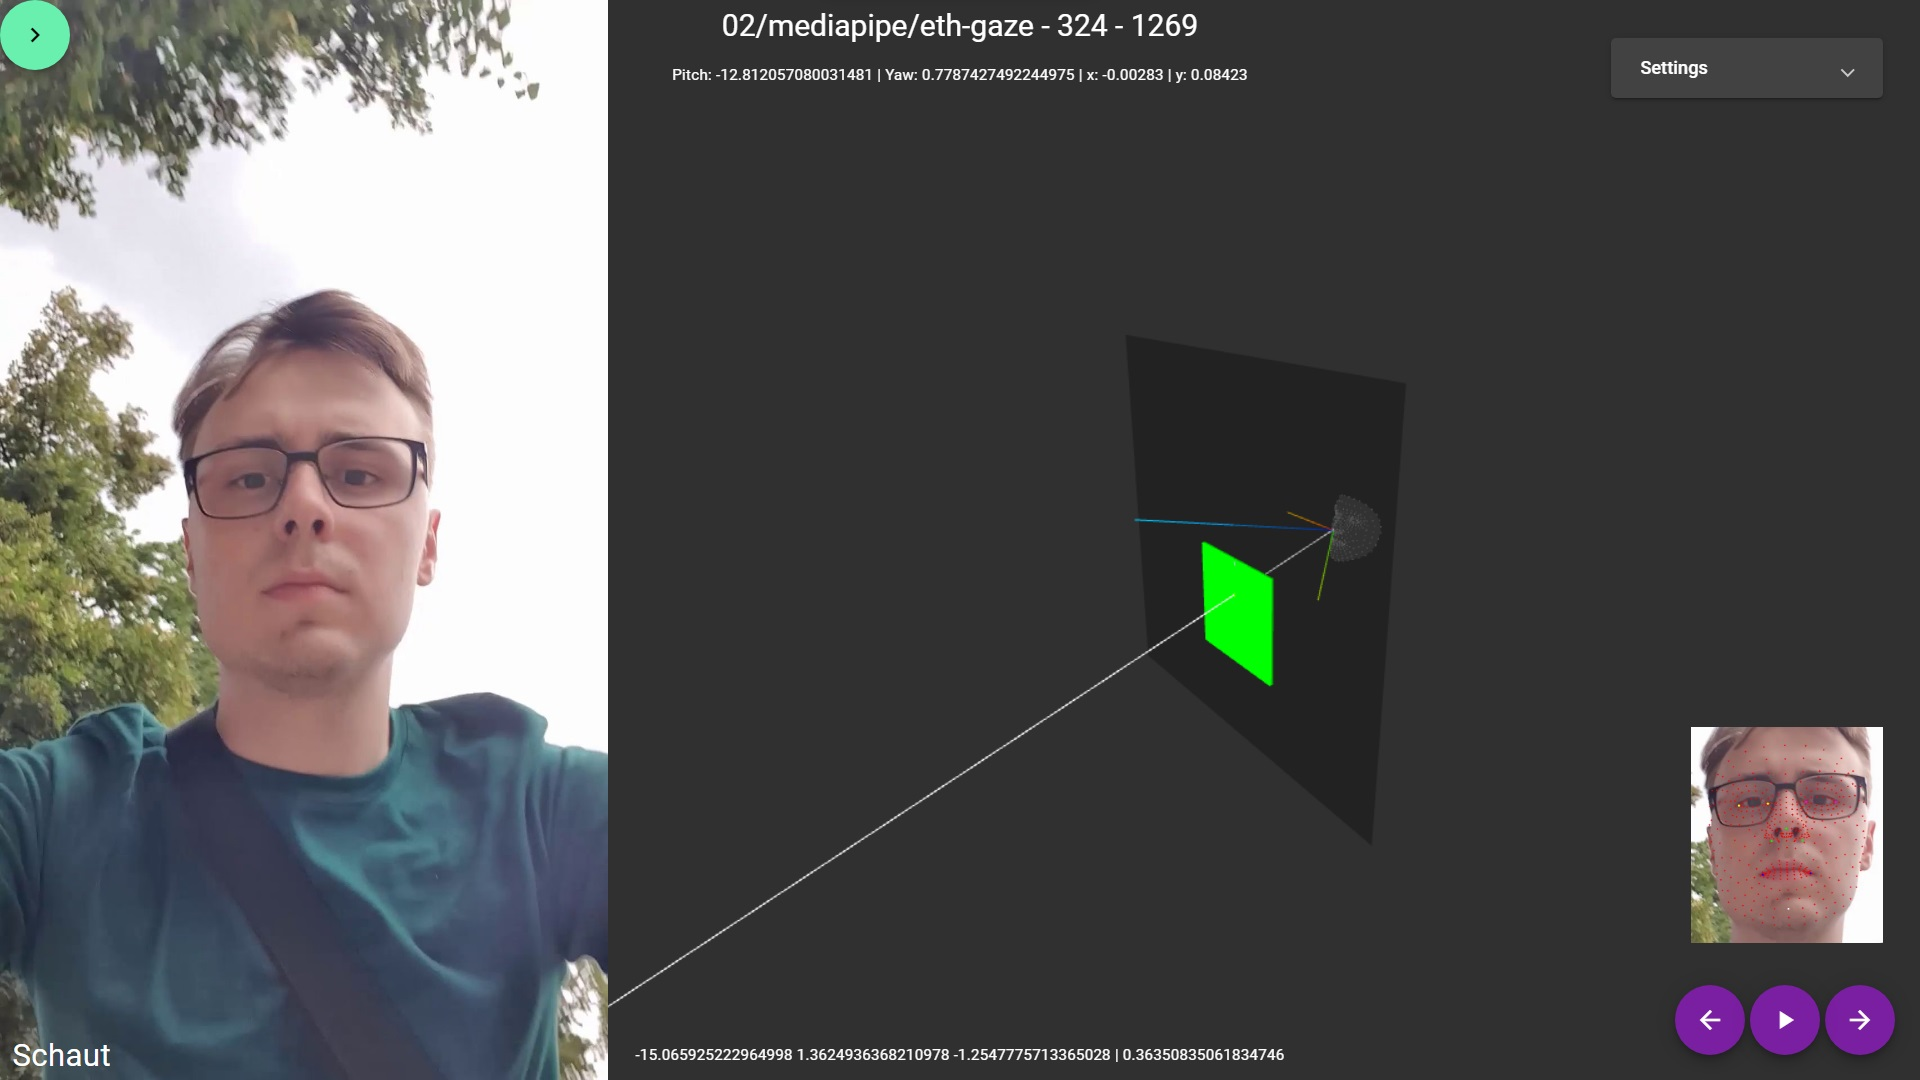
\includegraphics[width=\linewidth]{debug.jpg}
    \caption{Ansicht zur Analyse der Gesichtserkennung und Blickrichtungsbestimmung.}
    \label{fig:evaluation:debug}
\end{figure}

\section{Ergebnisse}\label{sec:evaluation:results}

In diesem Kapitel werden die Ergebnisse der Evaluation vorgestellt. Zunächst werden die Ergebnisse der Gesichtserkennung mit \dlib und \mediapipe diskutiert. Anschließend werden die Erkenntnisse der Analyse der Blickrichtungsbestimmung vorgestellt.

\subsection{Ergebnisse Gesichtserkennung}\label{sec:evaluation:results:face}

\begin{figure}
    \centering
    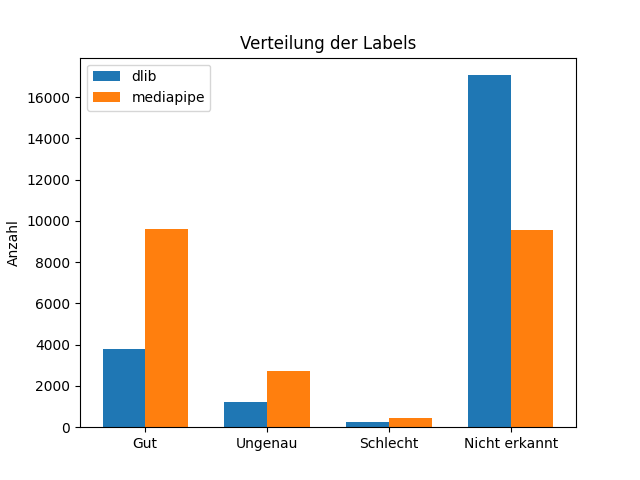
\includegraphics[width=0.7\linewidth]{evaluation/total-bar-quality.png}
    \caption{Gesamtzahl der Vorkommen der einzelnen Kategorien für \dlib und \mediapipe.}
    \label{fig:evaluation:total:quality}
\end{figure}

Nachdem die Qualität der Gesichtserkennung manuell bewertet wurde, können die Ergebnisse der beiden Gesichtserkennungsmethoden \dlib und \mediapipe verglichen werden. Abbildung \ref{fig:evaluation:total:quality} zeigt die Gesamtzahl der Vorkommen der einzelnen Kategorien sowohl für \dlib als auch für \mediapipe. Es ist zu erkennen, dass \mediapipe generell in deutlich mehr Bildern ein Gesicht erkennt als \dlib. Die genauen Vorkommen der Kategorien in den einzelnen Videos sind im Anhang zu finden.

Um die Gesamtqualität der erkannten Gesichter zwischen den Videos vergleichen zu können, wird der \textit{Qualitätsscore} eingeführt. Dazu wird zunächst eine Funktion $q$ definiert, die der Qualitätskategorie eines Frames einen numerischen Wert zuteilt. Die Funktion $q$ kann wie folgt beschrieben werden:

\[
q(Kategorie) = 
\begin{cases} 
0 & \text{wenn } Kategorie = schlecht \\
0,5 & \text{wenn } Kategorie = ungenau \\
1 & \text{wenn } Kategorie = gut \\
\end{cases}
\]

Der \textit{Qualitätsscore} ist dann der Durchschnitt der ermittelten Werte für alle erkannten Gesichter des Videos. 

In Kapitel \ref{sec:concept:head} wurde die These aufgestellt, dass wenn kein Gesicht im Bild erkannt werden kann, die Person auch nicht auf das Smartphone schaut. Dies wird vermutet, da erste Tests gezeigt haben, dass die Gesichtserkennung umso schlechter wird, je weiter der Kopf entlang der Querachse nach oben gedreht wird. Dies ist der Fall, wenn Radfahrende auf den Straßenverkehr schauen. Wenn sie jedoch auf ihr Smartphone schauen, neigen sie ihren Kopf in Richtung des Smartphone-Displays, wodurch die Gesichtserkennung besser funktioniert. Diese These soll in der Auswertung überprüft werden, indem untersucht wird, in wie vielen Bildern, in denen die Person auf das Smartphone schaut, ein Gesicht erkannt werden kann. Dazu wird der Bewertungsfaktor $\lambda$ eingeführt. Dieser gibt den prozentualen Anteil der Bilder, bei denen die Person auf das Smartphone schaut und gleichzeitig ein Gesicht erkannt wird ($N_{\text{Smartphone, Gesicht}}$), an der Gesamtzahl der Bilder an, bei denen die Person auf das Smartphone schaut ($N_{\text{Smartphone}}$). 

\[
\lambda = \frac{N_{\text{Smartphone,Gesicht}}}{N_{\text{Smartphone}}}\cdot 100
\]

Ein Wert von 100\% bedeutet, dass jedes Mal, wenn die Person auf das Smartphone geschaut hat, ein Gesicht erkannt werden konnte. Ein Wert von 0\% bedeutet, dass in keinem der Bilder, in denen die Person auf das Smartphone schaut, ein Gesicht erkannt werden konnte.

Die Tabelle \ref{tab:evaluation:face:scores} gibt einen Überblick über die Gesichtserkennung der einzelnen Videos. In der Tabelle wird angegeben:

\begin{itemize}
    \item der prozentuale Anteil der Bilder, in denen die Person auf das Smartphone sieht,
    \item der prozentuale Anteil der Bilder, in denen ein Gesicht erkannt wurde,
    \item der Wert $\lambda$, inklusive der Differenz von $N_{\text{Smartphone}}$ und $N_{\text{Smartphone, Gesicht}}$ 
    \item sowie der Qualitätsscore.
\end{itemize}

\begin{table}[]
    \centering
    \begin{tabular}{c | c | c  c c | c c c}
    \toprule
    & & \multicolumn{3}{c|}{\textbf{dlib}} & \multicolumn{3}{c}{\textbf{MediaPipe}} \\
    \midrule 
    Video 
    & \makecell{Auf\\Smartphone\\gesehen (\%)}
    & \makecell{Gesicht\\erkannt\\(\%)} 
    &  $\lambda$
    & \makecell{Qualitäts-\\Score}
    & \makecell{Gesicht\\erkannt\\(\%)}
    & $\lambda$
    & \makecell{Qualitäts-\\Score} 
    \\
    \hline 
01 & \cellcolor[HTML]{D1D1D1}\textcolor{black}{18,28} & \cellcolor[HTML]{BE4100}\textcolor{white}{25,42} & \cellcolor[HTML]{14EB00}\textcolor{black}{91,95 (7)} & \cellcolor[HTML]{2BD300}\textcolor{black}{0,83}& \cellcolor[HTML]{3EC100}\textcolor{black}{75,63} & \cellcolor[HTML]{01FD00}\textcolor{black}{98,85 (1)} & \cellcolor[HTML]{07F800}\textcolor{black}{0,97} \\
02 & \cellcolor[HTML]{DCDCDC}\textcolor{black}{13,71} & \cellcolor[HTML]{BA4500}\textcolor{white}{27,19} & \cellcolor[HTML]{0DF200}\textcolor{black}{94,83 (3)} & \cellcolor[HTML]{22DC00}\textcolor{black}{0,86}& \cellcolor[HTML]{3DC200}\textcolor{black}{75,89} & \cellcolor[HTML]{00FF00}\textcolor{black}{100,0 (0)} & \cellcolor[HTML]{0CF300}\textcolor{black}{0,95} \\
03 & \cellcolor[HTML]{E9E9E9}\textcolor{black}{8,72} & \cellcolor[HTML]{C83700}\textcolor{white}{21,79} & \cellcolor[HTML]{07F800}\textcolor{black}{97,22 (1)} & \cellcolor[HTML]{2ED100}\textcolor{black}{0,82}& \cellcolor[HTML]{1FE000}\textcolor{black}{87,89} & \cellcolor[HTML]{00FF00}\textcolor{black}{100,0 (0)} & \cellcolor[HTML]{18E600}\textcolor{black}{0,9} \\
04 & \cellcolor[HTML]{DEDEDE}\textcolor{black}{12,95} & \cellcolor[HTML]{649B00}\textcolor{black}{60,76} & \cellcolor[HTML]{00FF00}\textcolor{black}{100,0 (0)} & \cellcolor[HTML]{22DC00}\textcolor{black}{0,86}& \cellcolor[HTML]{02FC00}\textcolor{black}{98,48} & \cellcolor[HTML]{00FF00}\textcolor{black}{100,0 (0)} & \cellcolor[HTML]{1CE300}\textcolor{black}{0,89} \\
05 & \cellcolor[HTML]{CFCFCF}\textcolor{black}{19,12} & \cellcolor[HTML]{B64900}\textcolor{white}{28,57} & \cellcolor[HTML]{1CE300}\textcolor{black}{89,01 (10)} & \cellcolor[HTML]{20DE00}\textcolor{black}{0,87}& \cellcolor[HTML]{31CD00}\textcolor{black}{80,46} & \cellcolor[HTML]{01FD00}\textcolor{black}{98,9 (1)} & \cellcolor[HTML]{38C700}\textcolor{black}{0,78} \\
06 & \cellcolor[HTML]{C1C1C1}\textcolor{black}{24,44} & \cellcolor[HTML]{2ED100}\textcolor{black}{81,78} & \cellcolor[HTML]{00FF00}\textcolor{black}{100,0 (0)} & \cellcolor[HTML]{01FD00}\textcolor{black}{0,99}& \cellcolor[HTML]{00FF00}\textcolor{black}{100,0} & \cellcolor[HTML]{00FF00}\textcolor{black}{100,0 (0)} & \cellcolor[HTML]{00FF00}\textcolor{black}{1,0} \\
07 & \cellcolor[HTML]{DEDEDE}\textcolor{black}{12,91} & \cellcolor[HTML]{DB2400}\textcolor{white}{14,17} & \cellcolor[HTML]{7B8300}\textcolor{white}{51,75 (55)} & \cellcolor[HTML]{8F7000}\textcolor{white}{0,44}& \cellcolor[HTML]{798500}\textcolor{white}{52,0} & \cellcolor[HTML]{00FF00}\textcolor{black}{100,0 (0)} & \cellcolor[HTML]{30CF00}\textcolor{black}{0,81} \\
08 & \cellcolor[HTML]{EDEDED}\textcolor{black}{7,26} & \cellcolor[HTML]{CD3200}\textcolor{white}{19,6} & \cellcolor[HTML]{55AA00}\textcolor{black}{66,67 (29)} & \cellcolor[HTML]{30CF00}\textcolor{black}{0,81}& \cellcolor[HTML]{34CB00}\textcolor{black}{79,32} & \cellcolor[HTML]{00FF00}\textcolor{black}{100,0 (0)} & \cellcolor[HTML]{26D900}\textcolor{black}{0,85} \\
09 & \cellcolor[HTML]{EDEDED}\textcolor{black}{7,25} & \cellcolor[HTML]{E91600}\textcolor{white}{8,96} & \cellcolor[HTML]{09F500}\textcolor{black}{95,8 (5)} & \cellcolor[HTML]{18E600}\textcolor{black}{0,9}& \cellcolor[HTML]{D32B00}\textcolor{white}{17,0} & \cellcolor[HTML]{00FF00}\textcolor{black}{100,0 (0)} & \cellcolor[HTML]{51AE00}\textcolor{black}{0,68} \\
10 & \cellcolor[HTML]{DDDDDD}\textcolor{black}{13,58} & \cellcolor[HTML]{E21D00}\textcolor{white}{11,65} & \cellcolor[HTML]{2CD300}\textcolor{black}{82,43 (26)} & \cellcolor[HTML]{32CC00}\textcolor{black}{0,8}& \cellcolor[HTML]{D92600}\textcolor{white}{14,95} & \cellcolor[HTML]{00FF00}\textcolor{black}{100,0 (0)} & \cellcolor[HTML]{00FF00}\textcolor{black}{1,0} \\
11 & \cellcolor[HTML]{D0D0D0}\textcolor{black}{18,64} & \cellcolor[HTML]{BB4400}\textcolor{white}{26,8} & \cellcolor[HTML]{20DE00}\textcolor{black}{87,07 (57)} & \cellcolor[HTML]{39C500}\textcolor{black}{0,77}& \cellcolor[HTML]{54AB00}\textcolor{black}{67,16} & \cellcolor[HTML]{04FB00}\textcolor{black}{98,19 (8)} & \cellcolor[HTML]{28D700}\textcolor{black}{0,84} \\
12 & \cellcolor[HTML]{EAEAEA}\textcolor{black}{8,45} & \cellcolor[HTML]{D92600}\textcolor{white}{14,85} & \cellcolor[HTML]{07F800}\textcolor{black}{96,97 (4)} & \cellcolor[HTML]{38C700}\textcolor{black}{0,78}& \cellcolor[HTML]{649B00}\textcolor{black}{60,88} & \cellcolor[HTML]{00FF00}\textcolor{black}{100,0 (0)} & \cellcolor[HTML]{30CF00}\textcolor{black}{0,81} \\
13 & \cellcolor[HTML]{E1E1E1}\textcolor{black}{11,97} & \cellcolor[HTML]{DB2400}\textcolor{white}{14,39} & \cellcolor[HTML]{1EE100}\textcolor{black}{87,98 (44)} & \cellcolor[HTML]{22DC00}\textcolor{black}{0,86}& \cellcolor[HTML]{8C7300}\textcolor{white}{44,93} & \cellcolor[HTML]{00FF00}\textcolor{black}{99,73 (1)} & \cellcolor[HTML]{28D700}\textcolor{black}{0,84} \\
14 & \cellcolor[HTML]{D7D7D7}\textcolor{black}{15,95} & \cellcolor[HTML]{E11E00}\textcolor{white}{11,78} & \cellcolor[HTML]{659A00}\textcolor{black}{60,4 (80)} & \cellcolor[HTML]{10EE00}\textcolor{black}{0,93}& \cellcolor[HTML]{619D00}\textcolor{black}{61,7} & \cellcolor[HTML]{22DC00}\textcolor{black}{86,14 (28)} & \cellcolor[HTML]{39C500}\textcolor{black}{0,77} \\
15 & \cellcolor[HTML]{C9C9C9}\textcolor{black}{21,47} & \cellcolor[HTML]{B74800}\textcolor{white}{28,28} & \cellcolor[HTML]{00FF00}\textcolor{black}{100,0 (0)} & \cellcolor[HTML]{20DE00}\textcolor{black}{0,87}& \cellcolor[HTML]{38C700}\textcolor{black}{77,76} & \cellcolor[HTML]{00FF00}\textcolor{black}{100,0 (0)} & \cellcolor[HTML]{1CE300}\textcolor{black}{0,89} \\
16 & \cellcolor[HTML]{ECECEC}\textcolor{black}{7,63} & \cellcolor[HTML]{E21D00}\textcolor{white}{11,45} & \cellcolor[HTML]{00FF00}\textcolor{black}{100,0 (0)} & \cellcolor[HTML]{38C700}\textcolor{black}{0,78}& \cellcolor[HTML]{B64900}\textcolor{white}{28,63} & \cellcolor[HTML]{00FF00}\textcolor{black}{100,0 (0)} & \cellcolor[HTML]{35CA00}\textcolor{black}{0,79} \\
17 & \cellcolor[HTML]{CBCBCB}\textcolor{black}{20,47} & \cellcolor[HTML]{C63800}\textcolor{white}{22,43} & \cellcolor[HTML]{24DB00}\textcolor{black}{85,63 (24)} & \cellcolor[HTML]{10EE00}\textcolor{black}{0,93}& \cellcolor[HTML]{A15E00}\textcolor{white}{36,76} & \cellcolor[HTML]{04FB00}\textcolor{black}{98,2 (3)} & \cellcolor[HTML]{22DC00}\textcolor{black}{0,86} \\
18 & \cellcolor[HTML]{E2E2E2}\textcolor{black}{11,4} & \cellcolor[HTML]{BA4500}\textcolor{white}{27,08} & \cellcolor[HTML]{0FF000}\textcolor{black}{93,75 (6)} & \cellcolor[HTML]{2ED100}\textcolor{black}{0,82}& \cellcolor[HTML]{2DD200}\textcolor{black}{82,19} & \cellcolor[HTML]{01FD00}\textcolor{black}{98,96 (1)} & \cellcolor[HTML]{10EE00}\textcolor{black}{0,93} \\
19 & \cellcolor[HTML]{D3D3D3}\textcolor{black}{16,83} & \cellcolor[HTML]{916E00}\textcolor{white}{43,21} & \cellcolor[HTML]{00FF00}\textcolor{black}{100,0 (0)} & \cellcolor[HTML]{30CF00}\textcolor{black}{0,81}& \cellcolor[HTML]{17E800}\textcolor{black}{91,01} & \cellcolor[HTML]{00FF00}\textcolor{black}{100,0 (0)} & \cellcolor[HTML]{26D900}\textcolor{black}{0,85} \\
20 & \cellcolor[HTML]{B3B3B3}\textcolor{black}{29,34} & \cellcolor[HTML]{8C7300}\textcolor{white}{45,11} & \cellcolor[HTML]{0EF100}\textcolor{black}{94,34 (18)} & \cellcolor[HTML]{0FF000}\textcolor{black}{0,94}& \cellcolor[HTML]{2BD300}\textcolor{black}{82,84} & \cellcolor[HTML]{00FF00}\textcolor{black}{100,0 (0)} & \cellcolor[HTML]{17E800}\textcolor{black}{0,91} \\
21 & \cellcolor[HTML]{A3A3A3}\textcolor{black}{35,75} & \cellcolor[HTML]{699500}\textcolor{black}{58,29} & \cellcolor[HTML]{09F500}\textcolor{black}{96,03 (11)} & \cellcolor[HTML]{10EE00}\textcolor{black}{0,93}& \cellcolor[HTML]{27D800}\textcolor{black}{84,72} & \cellcolor[HTML]{00FF00}\textcolor{black}{100,0 (0)} & \cellcolor[HTML]{17E800}\textcolor{black}{0,91} \\
22 & \cellcolor[HTML]{C2C2C2}\textcolor{black}{24,09} & \cellcolor[HTML]{B54900}\textcolor{white}{29,0} & \cellcolor[HTML]{768900}\textcolor{white}{53,59 (71)} & \cellcolor[HTML]{4FB000}\textcolor{black}{0,69}& \cellcolor[HTML]{B54900}\textcolor{white}{29,16} & \cellcolor[HTML]{728C00}\textcolor{white}{54,9 (69)} & \cellcolor[HTML]{39C500}\textcolor{black}{0,77} \\
23 & \cellcolor[HTML]{EAEAEA}\textcolor{black}{8,26} & \cellcolor[HTML]{DD2200}\textcolor{white}{13,43} & \cellcolor[HTML]{1FE000}\textcolor{black}{87,8 (5)} & \cellcolor[HTML]{51AE00}\textcolor{black}{0,68}& \cellcolor[HTML]{E11E00}\textcolor{white}{11,78} & \cellcolor[HTML]{25DA00}\textcolor{black}{85,37 (6)} & \cellcolor[HTML]{32CC00}\textcolor{black}{0,8} \\
24 & \cellcolor[HTML]{CDCDCD}\textcolor{black}{19,69} & \cellcolor[HTML]{BB4400}\textcolor{white}{26,77} & \cellcolor[HTML]{0FF000}\textcolor{black}{93,86 (7)} & \cellcolor[HTML]{619E00}\textcolor{black}{0,62}& \cellcolor[HTML]{B94600}\textcolor{white}{27,63} & \cellcolor[HTML]{2CD300}\textcolor{black}{82,46 (20)} & \cellcolor[HTML]{0CF300}\textcolor{black}{0,95} \\

\hline
& & 28,03 & 87,74 & 0,82 & 61,2 & 95,90 & 0,86 \\
        \bottomrule
    \end{tabular}
    \caption{Übersicht über die Ergebnisse der Auswertung der Gesichtserkennung.}
    \label{tab:evaluation:face:scores}
\end{table}

Wie bereits erwähnt, wird deutlich, dass \dlib in wesentlich weniger Bildern ein Gesicht erkennt als \mediapipe. Überdurchschnittlich viele Gesichter erkennt \dlib in Video 06, allerdings ist dies das Video, in dem die Person nicht auf dem Fahrrad sondern auf einer Bank sitzt. Dabei sei angemerkt, dass \mediapipe in diesem Video in jedem Frame ein Gesicht erkennen kann, während \dlib nur in 81,78\% der Fälle ein Gesicht erkennt. Außerdem können mit \dlib viele Gesichter in den Videos 04 und 21 erkannt werden. Bei Video 04 handelt es sich um ein Video, in dem eine Person über einen sehr holprigen Untergrund fährt. Der Blick der Person ist daher größtenteils direkt auf die Fahrbahn vor ihr gerichtet, wodurch die allgemeine Kopfdrehung entlang der Querachse nicht so groß ist wie in den anderen Videos. Bei Video 21 ist zu erkennen, dass die Person in diesem Video prozentual am häufigsten auf das Display des Smartphones schaut. Dadurch ist der Kopf in diesem Video häufiger nicht extrem geneigt, weshalb auch hier viele Gesichter erkannt werden können. Am schlechtesten funktioniert die Gesichtserkennung mit \dlib in Video 09. Dies ist ein Video von \philipp, das mit der in Abbildung \ref{fig:evaluation:philipp:halterung} dargestellten Smartphone-Halterung aufgenommen wurden. Dadurch ist der Kopf relativ zur Kamera noch extremer gedreht als in den anderen Videos. Deshalb wird nur ein Gesicht erkannt, wenn die Person den Kopf neigt, um auf das Smartphone zu schauen, wie in Abbildung \ref{fig:appendix:09:dlib} zu sehen ist.

Die Gesichtserkennung mit \mediapipe funktioniert überwiegend sehr gut. Wie bereits erwähnt, kann in Video 06 bei einer ruhenden Person für jedes Bild des Videos ein Gesicht erkannt werden. Die größten Probleme bei der Gesichtserkennung mit \mediapipe treten in den Videos 09 und 10 auf. Dabei handelt es sich um die Videos von \philipp, die, wie bereits beschrieben, durch eine spezielle Halterung einen schwierigen Blickwinkel auf die Person zeigen. Daher kann auch mit \mediapipe in diesen Videos fast ausschließlich nur ein Gesicht erkannt werden, wenn die Person auf das Smartphone schaut, wie in Abbildung \ref{fig:appendix:09:mediapipe} zu sehen ist. Außerdem hat \mediapipe Probleme mit der Gesichtserkennung in den Videos 22, 23 und 24. Diese Videos wurden bei Nacht aufgenommen, weshalb die dargestellten Personen nur sehr schlecht beleuchtet sind. Ein Beispiel dafür ist in Abbildung \ref{fig:evaluation:face:error:dark} zu sehen. Ein weiterer Fall, in dem \mediapipe vergleichbar wenige Gesichter erkennt, ist Video 16. Wie in Tabelle \ref{tab:evaluation:videos:1} zu sehen ist, handelt es sich dabei um das kürzeste der aufgenommenen Videos. Außerdem fällt auf, dass die Person in diesem Video nur in 7,63\% des Videos auf das Smartphone schaut. Daher ist die Kopfdrehung der Person in den meisten Bildern zu hoch, um ein Gesicht zu erkennen. Ein weiteres Problem zeigt sich in Video 17. In diesem Video wurde die Smartphone-Halterung am äußersten Rand des Lenkergriffs montiert. Dadurch hat die Innenkamera zusätzlich einen seitlichen Blickwinkel auf die Person, weshalb in weniger Bildern ein Gesicht erkannt werden kann.

Die durchschnittliche Qualität der erkannten Gesichter von \dlib und \mediapipe ist sehr ähnlich. Es fällt auf, dass die Qualität der erkannten Gesichter bei Nacht (Videos 22, 23 und 24) mit \mediapipe besser ist als bei \dlib. Den mit Abstand schlechtesten \textit{Qualitätsscore} hat Video 07 mit der Gesichtserkennung mit \dlib. Auffällig ist, dass die Person in diesem Video eine Sonnenbrille trägt.

Von insgesamt 22.339 Bildern erkennt \mediapipe auf 9.546 Bildern kein Gesicht. Bei \dlib sind es sogar 17.068 Bilder, in denen kein Gesicht erkannt werden kann. Wie die $\lambda$-Werte der Videos zeigen, wird jedoch fast immer ein Gesicht erkannt, wenn die Person auf das Smartphone schaut. \mediapipe erkennt in 95\% aller Bilder, in denen die Person auf das Smartphone schaut, ein Gesicht.  Dabei ist vor allem auffällig, dass die schlechten Lichtbedingungen von Video 22, 23 und 24 einen großen Anteil daran haben, dass kein Gesicht erkannt wurde, wenn die Person auf das Smartphone sieht. Ein weiteres Video, was bei der Betrachtung der $\lambda$-Werte mit der Gesichtserkennung von \mediapipe hervorsticht, ist das Video 14. In diesem Video befindet sich die Sonne direkt hinter der dargestellten Person, wie in Abbildung \ref{fig:evaluation:face:error:bright} zu sehen ist.  Damit können 123 der insgesamt 138 Bilder, die bei der Gesichtserkennung mit \mediapipe davon betroffen sind, auf die sehr schlechten Lichtbedingungen in diesen Videos zurückgeführt werden. Bei \dlib kann in 87,74\% Prozent der Bilder, bei denen die Person auf das Smartphone sieht, ein Gesicht erkannt werden. Die meisten Bilder, bei denen das nicht der Fall ist, stammen ebenfalls aus den Videos mit den außergewöhnlichen Lichtbedingungen (Video 14, 22, 23 und 24). Auch fällt auf, das viele dieser Bilder aus den Videos 07 und 10 stammen, in denen die jeweils dargestellte Person eine Sonnenbrille trägt. \mediapipe hat mit diesen Videos kein Problem. 

Die Annahme, dass wenn kein Gesicht erkannt wird, die Person nicht auf das Smartphone schaut, konnte somit in den meisten Fällen bestätigt werden. Für die weitere Auswertung wird daher angenommen, dass wenn auf einem Bild kein Gesicht erkannt und somit keine Blickrichtung bestimmt werden konnte, die Person auf diesen Bildern nicht auf das Smartphone sieht.

Darüber hinaus konnte in dieser Auswertung gezeigt werden, dass die Kopfdrehung sowohl bei \dlib als auch bei \mediapipe eine entscheidende Rolle bei der Gesichtserkennung spielt. Des Weiteren konnte gezeigt werden, dass extreme Lichtverhältnisse, wie sie in Abbildung \ref{fig:evaluation:face:score} zu sehen sind, sowie das Tragen einer Sonnenbrille die Gesichtserkennung beeinträchtigen. 

\begin{figure}{}
    \begin{subfigure}{0.3\textwidth}
        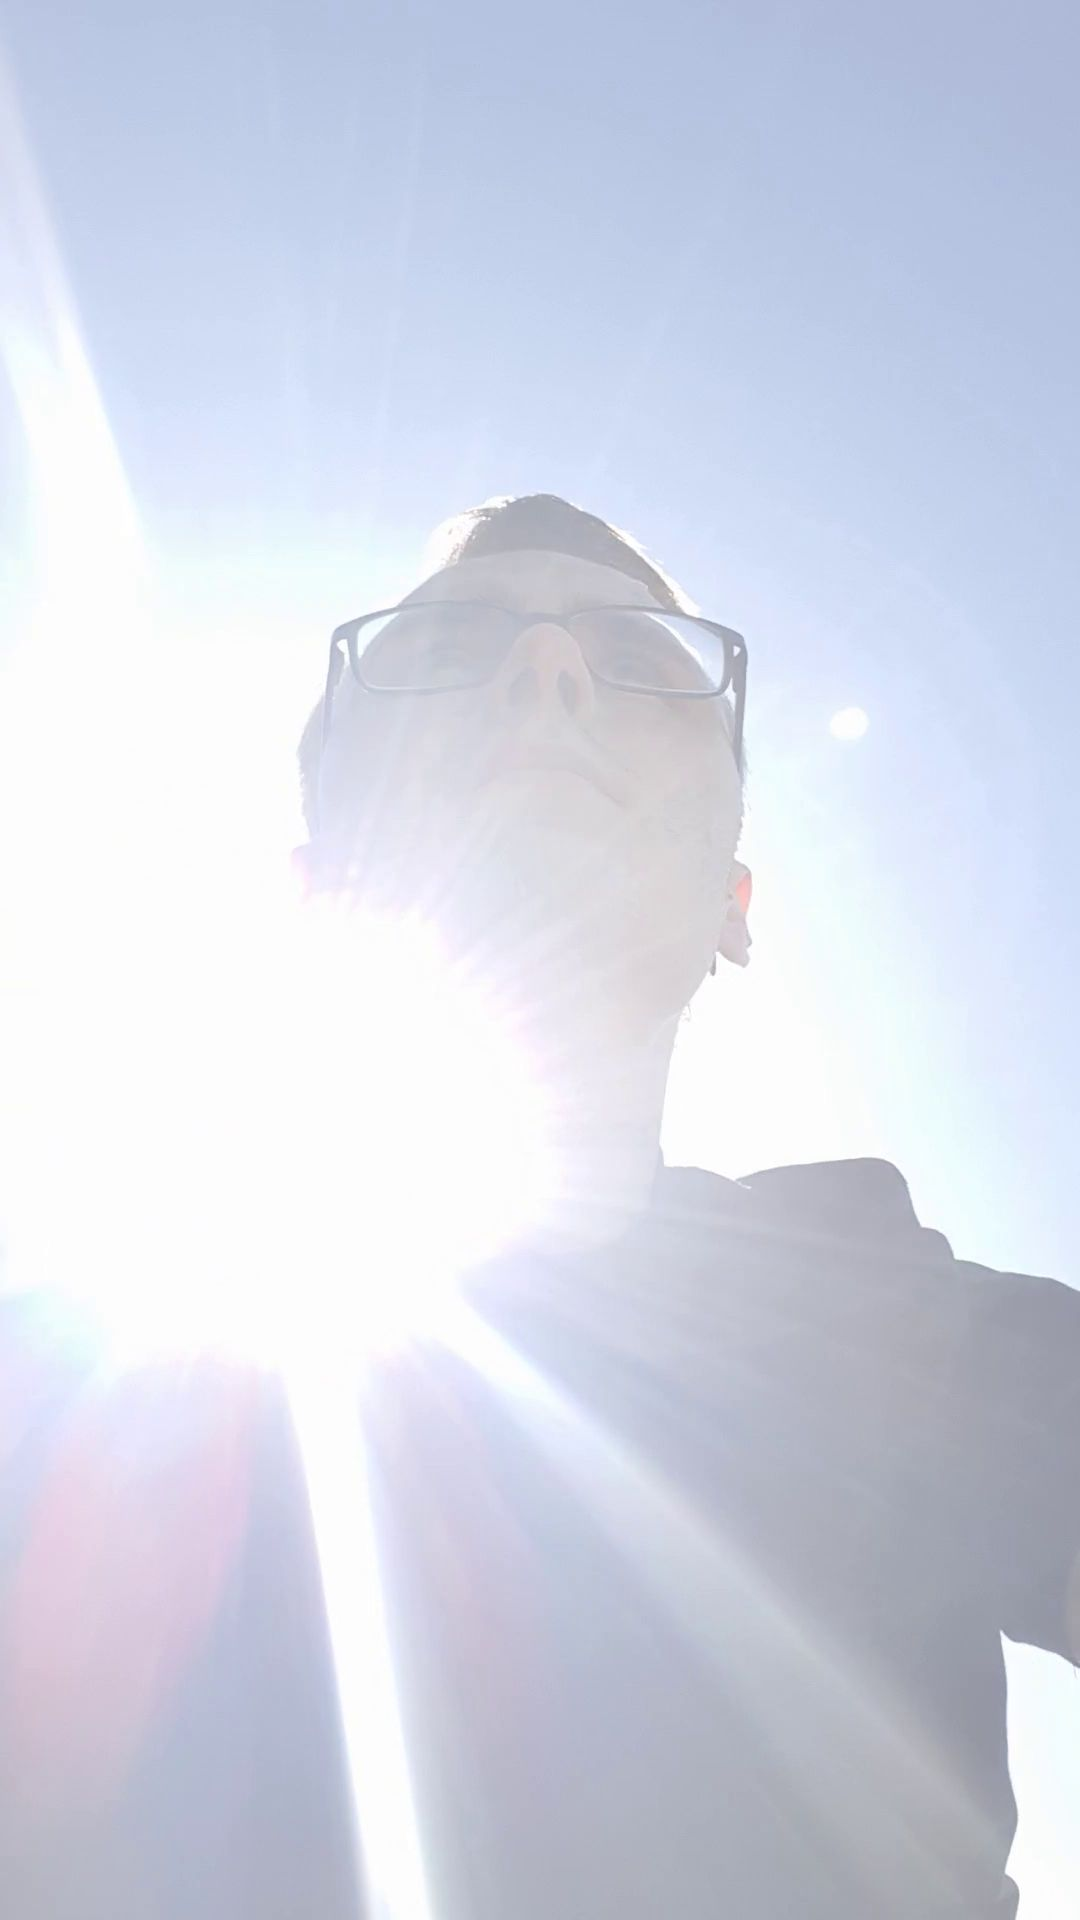
\includegraphics[width=\linewidth]{evaluation/face_error_bright.jpg}
        \caption{Beispiel für nicht erkanntes Gesicht wegen extremer Helligkeit.}
        \label{fig:evaluation:face:error:bright}
    \end{subfigure}
    \begin{subfigure}{0.3\textwidth}
        
\includegraphics[width=\linewidth]{evaluation/face_error_dark.jpg}
        \caption{Beispiel für nicht erkanntes Gesicht wegen extremer Dunkelheit.}
        \label{fig:evaluation:face:error:dark}
    \end{subfigure}
    \caption{Extreme Lichtverhältnisse, die das Erkennen von Gesichtern erschweren.}
    \label{fig:evaluation:face:score}
\end{figure}

Zusätzlich zu der bereits beschriebenen Auswertung wurde untersucht, welchen Einfluss der ermittelte Abstand des Gesichts zum Bildschirm $\distancefacecamera$ auf die Qualität der Gesichtserkennung hat. Dabei wurde festgestellt, dass ab einem bestimmten Grenzwert alle erkannten Gesichter als \textit{schlecht} eingestuft wurden, wie in Abbildung \ref{fig:evaluation:distance:total} zu sehen ist. Weiterhin wurde festgestellt, dass alle betroffenen Gesichter mit \dlib erkannt wurden, wie in Abbildung \ref{fig:evaluation:distance:model} zu sehen ist. Beispiele für solche erkannten Gesichter sind in Abbildung \ref{fig:evaluation:bad:distance} zu sehen. Diese Gesichter sollen daher bei der weiteren Betrachtung ignoriert werden. Der Grenzwert, den die Distanz $\distancefacecamera$ dabei nicht überschreiten darf, wurde anhand der Daten auf 1 festgelegt.

\begin{figure}
    \centering
    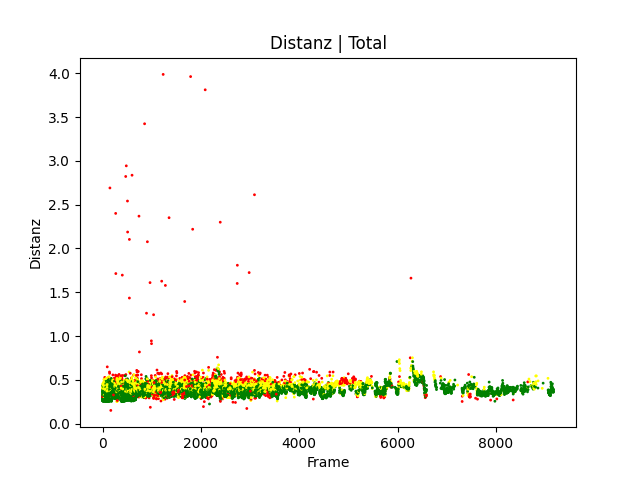
\includegraphics[width=0.7\linewidth]{evaluation/distance-total.png}
    \caption{Abhängigkeit der Qualität der Gesichtserkennung von der Distanz $\distancefacecamera$. Rot markiert sind die Gesichter, welche als \textit{schlecht erkannt} eingestuft wurden. Grün sind die Gesichter, die als \textit{gut erkannt} eingestuft wurden. Gelbe Punkte repräsentieren Gesichter, die als \textit{ungenau erkannt} eingestuft wurden.}
        \label{fig:evaluation:distance:total}
\end{figure}

\begin{figure}
    \centering
    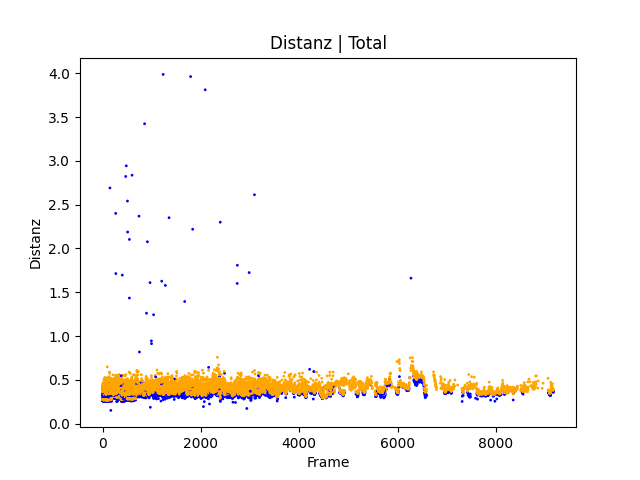
\includegraphics[width=0.7\linewidth]{evaluation/distance_model.png}
    \caption{Abhängigkeit der ermittelten Distanz $\distancefacecamera$ von der verwendeten Methode. Mit \dlib erkannte Gesichter werden blau dargestellt. Mit \mediapipe erkannte Gesichter werden orange dargestellt.}
    \label{fig:evaluation:distance:model}
\end{figure}



\begin{figure}[]
    \begin{subfigure}{0.425\textwidth}
        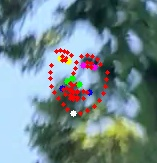
\includegraphics[width=\linewidth]{evaluation/bad_distance_1.jpg}
        \caption{Video 13, Frame 150, Distanz 2,69}
        \label{fig:evaluation:bad:distance:1}
    \end{subfigure}%
    \vspace{0.5cm}
    \begin{subfigure}{0.45\textwidth}
        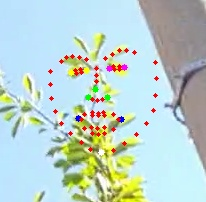
\includegraphics[width=\linewidth]{evaluation/bad_distance_2.jpg}
        \caption{Video 13, Frame 2739, Distanz 1,6}
        \label{fig:evaluation:bad:distance:2}
    \end{subfigure}
    \caption{Beispiele für Bilder, die als \textit{schlecht} eingestuft wurden und einen auffällig großen Abstand aufweisen.}
    \label{fig:evaluation:bad:distance}
\end{figure}

\subsection{Ergebnisse Blickrichtungsbestimmung}

Im Folgenden werden die Ergebnisse der Blickrichtungsbestimmung diskutiert. Dazu wird zunächst die Bestimmung der idealen Werte für die in Kapitel \ref{sec:implementation:gaze:interpretation} vorgestellte Seitenlänge $\hitthresholdsize$ und die Verschiebung $\hitthresholdposition$ beschrieben. Diese Werte werden für alle acht möglichen Kombinationen von Gesichtserkennung und Blickrichtungsbestimmung separat ermittelt. Basierend auf diesen Werten wird dann die Qualität der Blickrichtungsbestimmung für die einzelnen Videos analysiert, um zu untersuchen, wie gut verschiedene Umwelteinflüsse von den einzelnen Methoden zur Blickrichtungsbestimmung erkannt werden. Abschließend wird der Einfluss von geschlossenen Augen auf die Qualität der Blickrichtungsbestimmung diskutiert.

Generell wird für die Bewertung der Blickrichtung der F1-Score verwendet. Dazu wurde eine Ground Truth erstellt, die für jedes Bild angibt, ob die abgebildete Person auf das Smartphone schaut oder nicht. Als positive Instanzen werden alle Bilder verwendet, in denen die Person auf das Smartphone schaut (Kategorie A.1). Die negative Instanzen sind dann alle anderen Bilder, bei denen die Person nicht auf das Smartphone schaut (Kategorie A.0) oder bei denen das Gesicht der Person nicht im Bild erkenntlich ist (Kategorie A.2). Diese werden dann mit den Vorhersagen der einzelnen Methoden verglichen, um die \textit{True Positives} ($TP$), \textit{True Negatives} ($TN$), \textit{False Positives} ($FP$) und die \textit{False Negatives} ($FN$) zu ermitteln, anhand derer sich dann der F1-Score berechnet lässt. Aufgrund der Erkenntnisse aus Kapitel \ref{sec:evaluation:results:face} werden Bilder, bei denen das erkannte Gesicht einen Abstand von mehr als eins hat, bei der Berechnung des F1-Scores nicht berücksichtigt.

\subsubsection{Hyperparameter-Tuning}\label{sec:evaluation:results:gaze:threshold}

Um die idealen Werte für die Seitenlänge $\hitthresholdsize$ und die Verschiebung $\hitthresholdposition$ zu ermitteln, wurden zunächst erste Tests mit dem in Kapitel \ref{sec:evaluation:plan:tool} vorgestellten Anwendung zur Analyse der Daten durchgeführt, um ein grobes Intervall möglicher Werte für die Parameter $\hitthresholdsize$ und $\hitthresholdposition$ zu definieren. Dieser Test ergab die folgenden Intervalle:

\[
\hitthresholdsize \in [0,0.5] \qquad \hitthresholdposition \in [-0.1, 0.5]
\]

Diese Intervalle wurden in 50 gleich große Schritte unterteilt. Dann wurde für jede mögliche Kombination der Werte dieser Parameter der F1-Score für das Video berechnet. Diese wurden für jedes Video in einer Matrix gespeichert, wobei jede Kombination der Parameterwerte eine Zelle adressiert. Nach der Bearbeitung jedes Videos wurde der durchschnittliche F1-Score für alle diese Kombinationen berechnet. Ausgehend vom maximalen F1-Score wurden dann die Parameter $\hitthresholdsize$ und $\hitthresholdposition$ für jede mögliche Kombination von Gesichtserkennung und Blickrichtungsbestimmung ermittelt. 

Die aufgezeichneten Videos zeigen Faktoren, die bei der Analyse der Gesichtserkennung in Kapitel \ref{sec:evaluation:results:face} als hinderlich eingestuft wurden, die aber bei einer möglichen Studie im Rahmen der PrioBike-App beeinflusst werden können. So kann man den Teilnehmenden einer solchen Studie das Tragen von Sonnenbrillen verbieten. Des Weiteren hat man Einfluss auf die Tageszeit, zu der eine Studie stattfindet, weshalb extreme Dunkelheit in der Nacht vermieden werden kann. Daher wurde das oben beschriebene Verfahren erneut durchgeführt. Diesmal wurden jedoch einige Videos von der Betrachtung ausgeschlossen. Diese Videos waren:

\begin{itemize}
    \item Video 06, da \markus in diesem Video auf einer Bank sitzt und nicht auf dem Fahrrad,
    \item Video 07 und 10, da \paul und \philipp in diesen Videos eine Sonnenbrille tragen,
    \item Video 22, 23 und 24, da diese bei Nacht aufgenommen wurden.
\end{itemize}

Die besten Werte für die Parameter $\hitthresholdsize$ und $\hitthresholdposition$ der Blickrichtungsbestimmung mit Gesichtserkennung unter Verwendung von \dlib sind in den folgenden Abbildungen dargestellt:

\begin{itemize}
    \item  \textit{ETH-XGaze} in Abbildung  \ref{fig:evaluation:threshold:dlib:eth-gaze}
    \item  \textit{Gaze360} in Abbildung 
 \ref{fig:evaluation:threshold:dlib:l2cs-gaze-360}
    \item  \textit{MPIIFaceGaze} in Abbildung \ref{fig:evaluation:threshold:dlib:mpiifacegaze}
    \item  \textit{Kopfrotation} in Abbildung 
 \ref{fig:evaluation:threshold:dlib:head-rotation}
\end{itemize}

Für die Blickrichtungsbestimmung basierend auf der Gesichtserkennung mit \mediapipe sind die Parameter in den folgenden Abbildungen dargestellt:

\begin{itemize}
    \item  \textit{ETH-XGaze} in Abbildung \ref{fig:evaluation:threshold:mediapipe:eth-gaze}
    \item  \textit{Gaze360} in Abbildung \ref{fig:evaluation:threshold:mediapipe:l2cs-gaze-360}
    \item  \textit{MPIIFaceGaze} in Abbildung \ref{fig:evaluation:threshold:mediapipe:mpiifacegaze}
    \item  \textit{Kopfrotation} in Abbildung \ref{fig:evaluation:threshold:mediapipe:head-rotation}
\end{itemize}

Es ist zu beachten, dass zur Bestimmung dieser Werte größtenteils Videos verwendet wurden, die von derselben Person aufgenommen wurden. Auch wenn versucht wurde, in diesen Videos eine möglichst große Vielfalt darzustellen, können die ermittelten Parameter dadurch beeinflusst worden sein. Im Anhang sind die idealen Parameter und die entsprechenden maximalen F1-Scores aufgeführt, die speziell für jedes Video ermittelt wurden. 

In Tabelle \ref{tab:evaluation:results:gaze:best:f1} sind die maximalen F1-Scores für jede Kombination von Gesichtserkennung und Blickrichtungsbestimmung aufgeführt. Es ist zu erkennen, dass die Eliminierung von vermeidbaren Umwelteinflüssen den F1-Score für jede Kombination verbessert. Die einzige Ausnahme ist die Kombination aus \mediapipe mit \mpii. Generell ist zu erkennen, dass die Blickrichtungsbestimmung mit \mpii mit Abstand die schlechtesten Ergebnisse erzielte. Bei näherer Betrachtung der Daten fiel auf, dass mit \mpii der Schnittpunkt $\intersection$ bei jedem verarbeiteten Frame in der Nähe des Koordinatenursprungs liegt. Dies ist auch daran zu erkennen, dass die ermittelte Seitenlänge $\hitthresholdsize$ (siehe Abbildungen \ref{fig:evaluation:threshold:dlib:mpiifacegaze} und \ref{fig:evaluation:threshold:mediapipe:mpiifacegaze}) deutlich kleiner ist als bei den anderen Ansätzen. Daher wird in fast allen Bildern, in denen zuvor ein Gesicht erkannt wurde, festgestellt, dass die Person auf das Smartphone schaut. Dies ist auch in Abbildung \ref{fig:evaluation:gaze:mpiifacegaze} zu sehen. Diese zeigt die Ground Truth des Blickkontaktes, die Vorhersage des Blickkontaktes, die Qualität der erkannten Gesichter und ob ein Gesicht erkannt wurde.

\begin{figure}
    \centering
    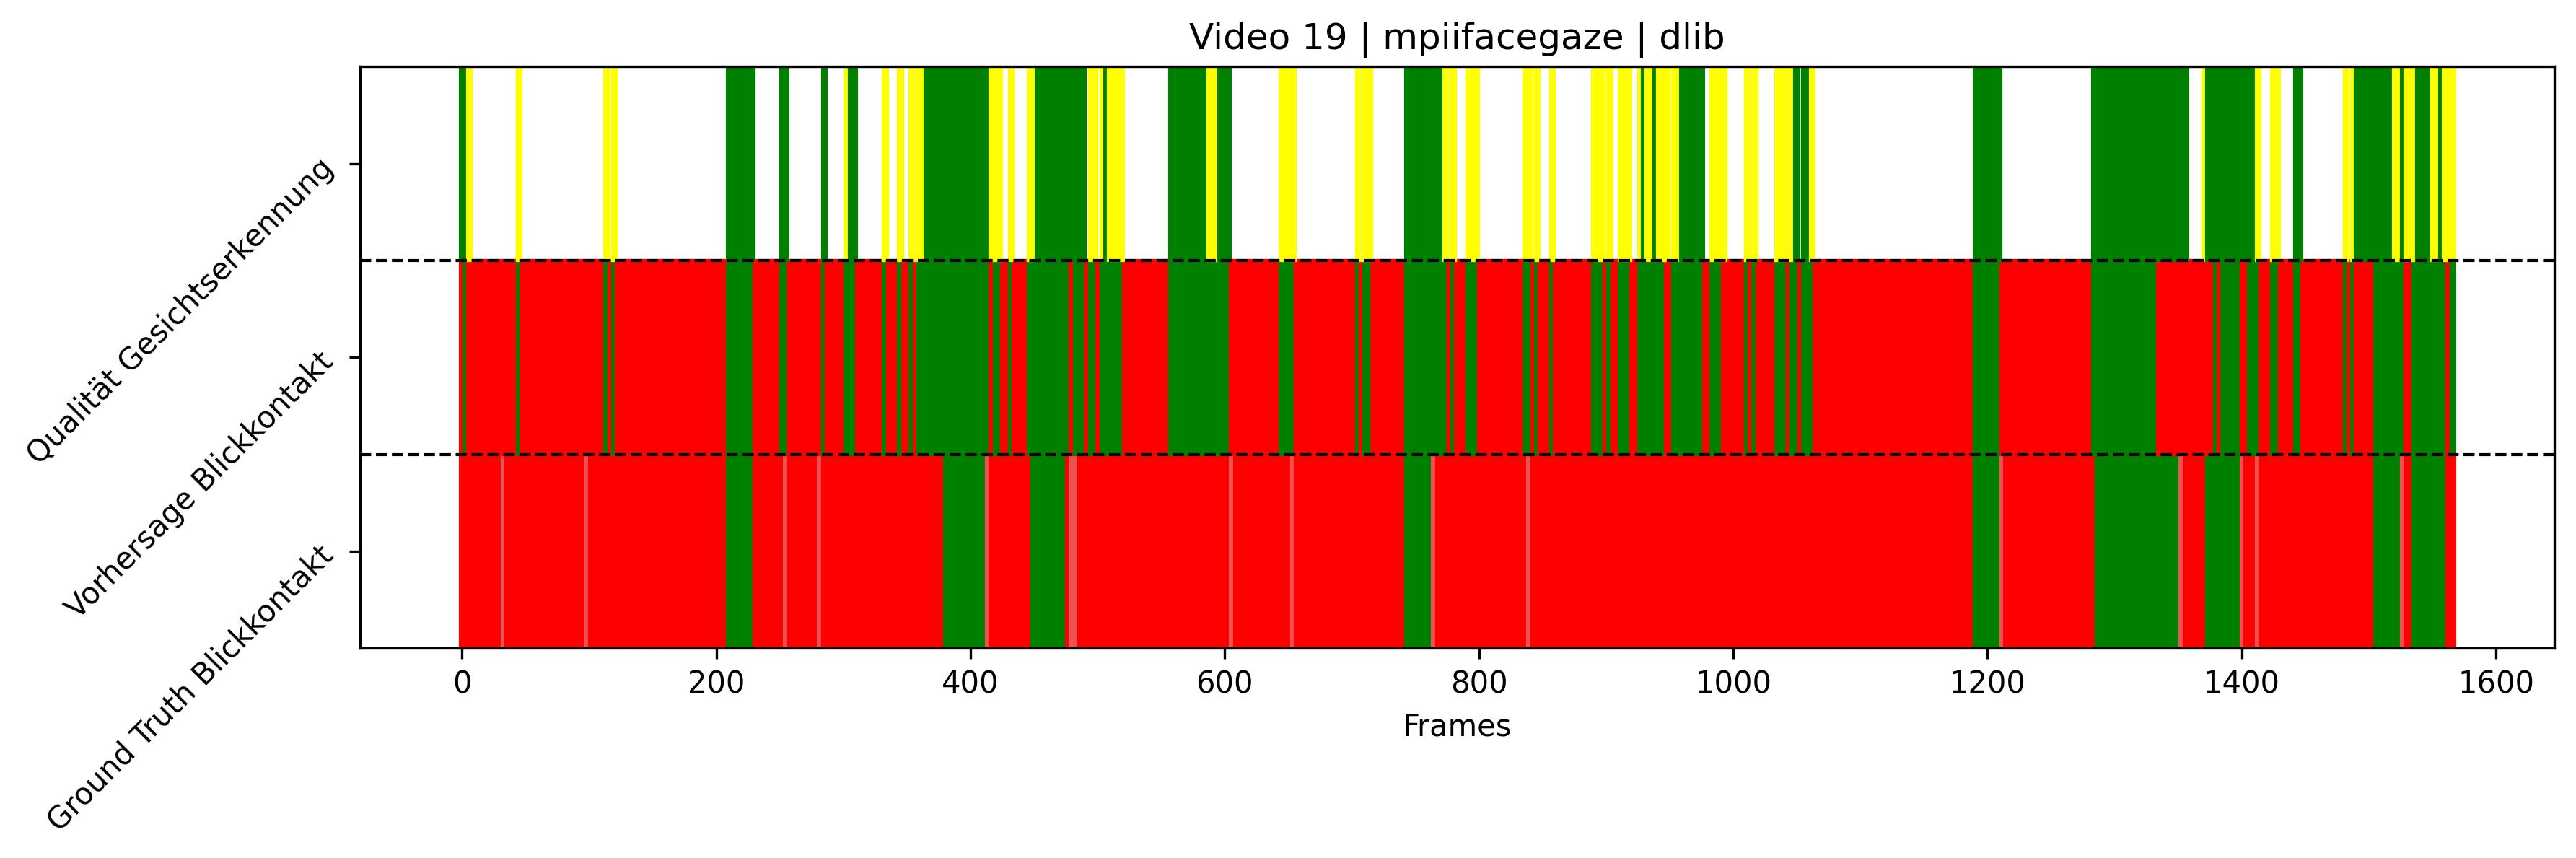
\includegraphics[width=\linewidth]{evaluation/19_dlib_mpiifacegaze.jpg}
    \caption{Übersicht über die Ground Truth des Blickkontakts, die Vorhersage des Blickkontakts und die Qualität der erkannten Gesichter. Bei der Gound Truth steht grün für die Kategorie A.1, rot für die Kategorie A.0 und rosa für die Kategorie A.2. Bei der Blickkontaktvorhersage bedeutet rot, dass die Person nicht auf das Smartphone schaut und grün, dass die Person auf das Smartphone schaut. Bei der Qualität der Gesichtserkennung steht rot für \textit{schlecht erkannt}, gelb für \textit{ungenau erkannt} und grün für \textit{gut erkannt}. Bilder, bei denen kein Gesicht erkannt wurde, werden nicht angezeigt. }
    \label{fig:evaluation:gaze:mpiifacegaze}
\end{figure}

Aufgrund der in Kapitel \ref{sec:evaluation:results:face} bestätigten Annahme, dass wenn kein Gesicht erkannt wird, die Person auch nicht auf das Smartphone schaut, erzielt dieser Ansatz bessere Ergebnisse, wenn nur in wenigen Bildern ein Gesicht erkannt wird. Da, wie in Kapitel \ref{sec:evaluation:results:face} gezeigt, \dlib generell weniger Gesichter erkennt, funktioniert der Ansatz mit \mpii am besten mit \dlib. Bereits bei der Konzeptentwicklung wurde vermutet, dass die Verwendung des \mpii-Datensatzes für die Bestimmung der Blickrichtung von Radfahrenden nicht geeignet ist, da der Datensatz nur Bilder von Personen enthält, die auf den Bildschirm eines Laptops schauen. Diese Vermutung konnte damit bestätigt werden.

Den mit Abstand besten F1-Score erreicht die Kombination aus Blickrichtungsbestimmung mit \ethg und Gesichtserkennung durch \mediapipe, direkt gefolgt von der Kombination aus \ethg und \dlib. Dies zeigt, dass der \ethg-Datensatz am besten geeignet ist, die Blickrichtung von Radfahrenden zu bestimmen. Der \gazed Datensatz erzielte ebenfalls gute Ergebnisse, wenn auch deutlich schlechter als der \ethg Datensatz. Weiterhin ist zu erkennen, dass die Blickrichtungsbestimmung aus der Kopfdrehung in Kombination mit \mediapipe ebenfalls gut für die Bestimmung der Blickrichtung von Radfahrenden geeignet ist.

\begin{table}[]
\begin{tabular}{l c c c c c}
\toprule
               & \textbf{Gesichtserkennung} & \textbf{ETH-XGaze} &\textbf{Gaze360}  & \textbf{MPIIFaceGaze} & \textbf{Kopfrotation} \\
\midrule
\multirowcell{2}{Alle Videos}   & dlib          & 0,855             & 0,732                & 0,686    & 0,703                     \\
                                & MediaPipe     & 0,874             & 0,708                & 0,493      & 0,797        \\
\midrule
\multirowcell{2}{Teilmenge\\der Videos} & dlib          & 0,91            & \textbf{0,848}        & \textbf{0,704}  & 0,729            \\
                                        & MediaPipe    & \textbf{0,928}    & 0,808                  & 0,439& \textbf{0,833}           \\
          \bottomrule
\caption{Maximaler durchschnittlicher F1-Score für die einzelnen Methoden zur Bestimmung der Blickrichtung mit unterschiedlicher Gesichtserkennungen als Grundlage.}
\label{tab:evaluation:results:gaze:best:f1}
\end{tabular}
\end{table}


\begin{figure}{}
    \begin{subfigure}{0.45\textwidth}
        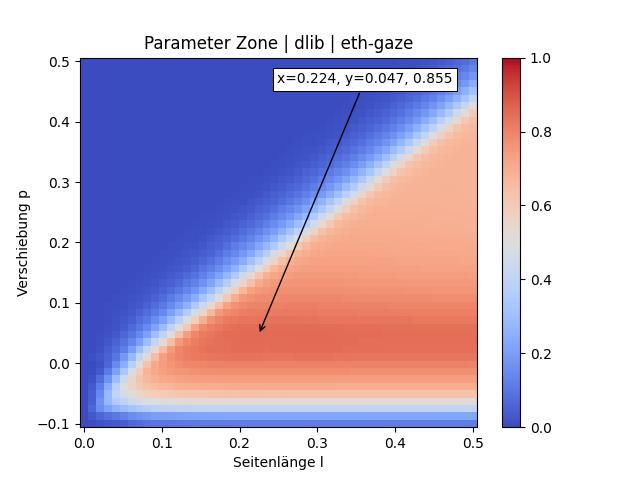
\includegraphics[width=\linewidth]{evaluation/dlib-eth-gaze-total-contour.jpg}
        \caption{Alle Videos}
        \label{fig:evaluation:threshold:dlib:eth-gaze:all}
    \end{subfigure}
    \begin{subfigure}{0.45\textwidth}
        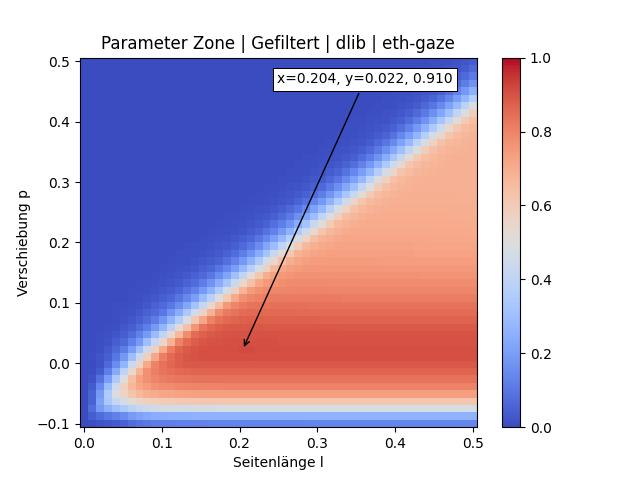
\includegraphics[width=\linewidth]{evaluation/dlib-eth-gaze-total-ignore-contour.jpg}
        \caption{Teilmenge der Videos}
        \label{fig:evaluation:threshold:dlib:eth-gaze:ignore}
    \end{subfigure}%
    \caption{Ergebnis des Hyperparameter-Tunings für die Gesichtserkennung mit \dlib und die Blickrichtungsbestimmung mit \ethg.}
    \label{fig:evaluation:threshold:dlib:eth-gaze}
\end{figure}
\begin{figure}{}
    \begin{subfigure}{0.45\textwidth}
        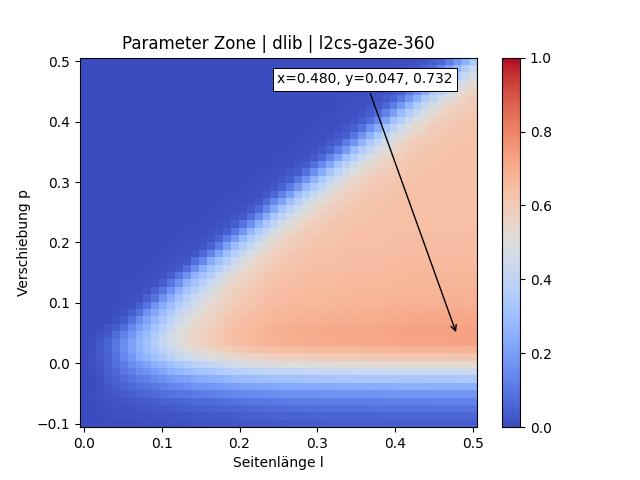
\includegraphics[width=\linewidth]{evaluation/dlib-l2cs-gaze-360-total-contour.jpg}
        \caption{Alle Videos}
        \label{fig:evaluation:threshold:dlib:l2cs-gaze-360:all}
    \end{subfigure}%
    \begin{subfigure}{0.45\textwidth}
        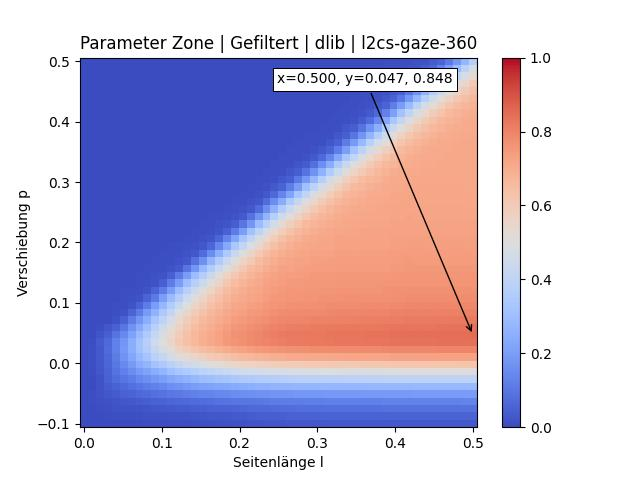
\includegraphics[width=\linewidth]{evaluation/dlib-l2cs-gaze-360-total-ignore-contour.jpg}
        \caption{Teilmenge der Videos}
        \label{fig:evaluation:threshold:dlib:l2cs-gaze-360:ignore}
    \end{subfigure}%
    \caption{Ergebnis des Hyperparameter-Tunings für die Gesichtserkennung mit \dlib und die Blickrichtungsbestimmung mit \gazed.}
    \label{fig:evaluation:threshold:dlib:l2cs-gaze-360}
\end{figure}
\begin{figure}{}
    \begin{subfigure}{0.45\textwidth}
        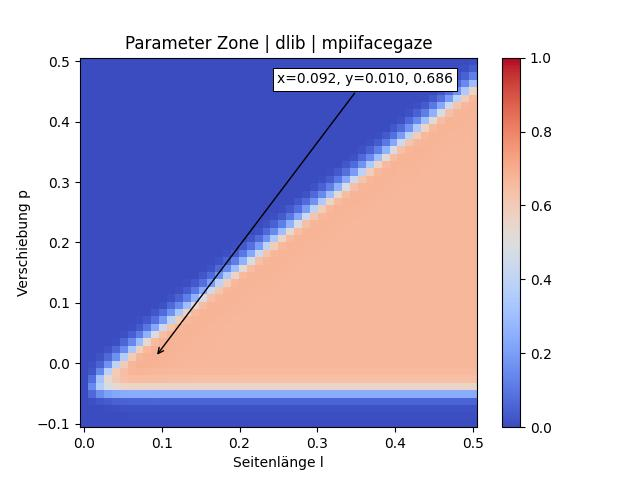
\includegraphics[width=\linewidth]{evaluation/dlib-mpiifacegaze-total-contour.jpg}
        \caption{Alle Videos}
        \label{fig:evaluation:threshold:dlib:mpiifacegaze:all}
    \end{subfigure}
    \begin{subfigure}{0.45\textwidth}
        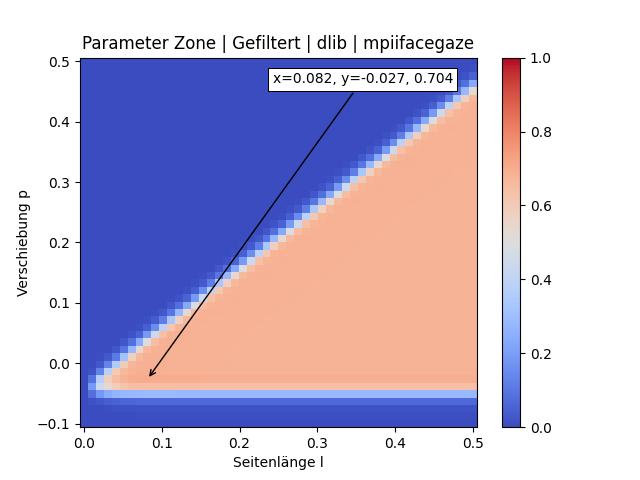
\includegraphics[width=\linewidth]{evaluation/dlib-mpiifacegaze-total-ignore-contour.jpg}
        \caption{Teilmenge der Videos}
        \label{fig:evaluation:threshold:dlib:mpiifacegaze:ignore}
    \end{subfigure}%
    \caption{Ergebnis des Hyperparameter-Tunings für die Gesichtserkennung mit \dlib und die Blickrichtungsbestimmung mit \mpii.}
    \label{fig:evaluation:threshold:dlib:mpiifacegaze}
\end{figure}
\begin{figure}{}
    \begin{subfigure}{0.45\textwidth}
        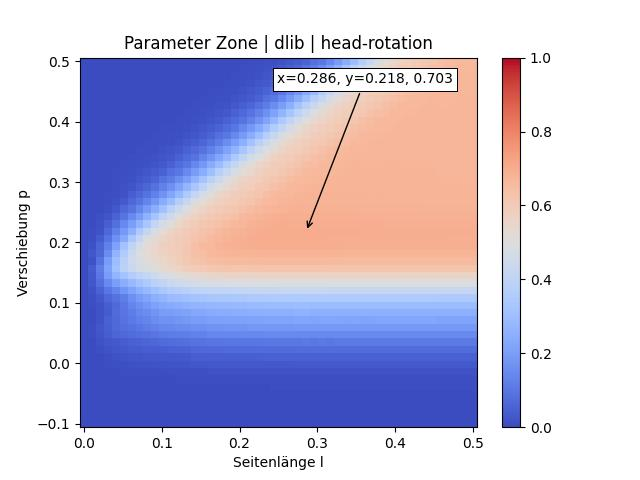
\includegraphics[width=\linewidth]{evaluation/dlib-head-rotation-total-contour.jpg}
        \caption{Alle Videos}
        \label{fig:evaluation:threshold:dlib:head-rotation:all}
    \end{subfigure}
    \begin{subfigure}{0.45\textwidth}
        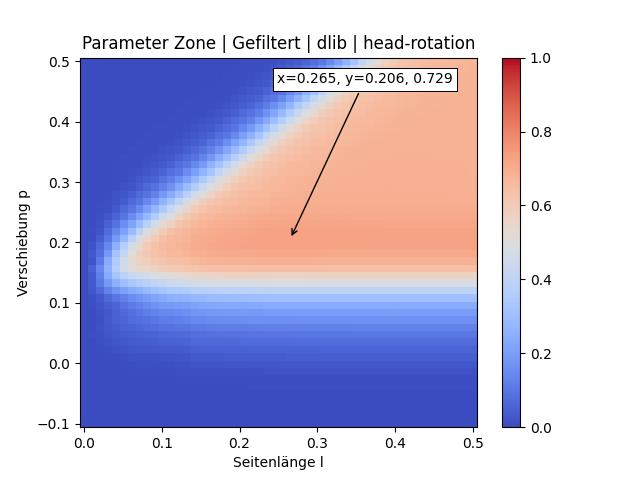
\includegraphics[width=\linewidth]{evaluation/dlib-head-rotation-total-ignore-contour.jpg}
        \caption{Teilmenge der Videos}
        \label{fig:evaluation:threshold:dlib:head-rotation:ignore}
    \end{subfigure}%
    \caption{Ergebnis des Hyperparameter-Tunings für die Gesichtserkennung mit \dlib und die Blickrichtungsbestimmung mittels der Kopfrotation.}
    \label{fig:evaluation:threshold:dlib:head-rotation}
\end{figure}

\begin{figure}{}
    \begin{subfigure}{0.45\textwidth}
        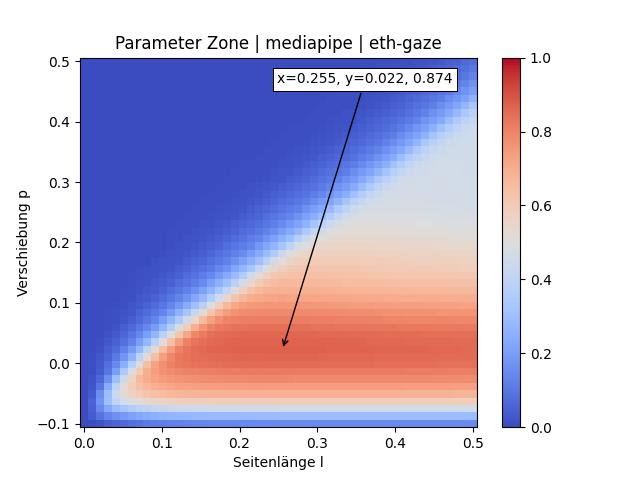
\includegraphics[width=\linewidth]{evaluation/mediapipe-eth-gaze-total-contour.jpg}
        \caption{Alle Videos}
        \label{fig:evaluation:threshold:mediapipe:eth-gaze:all}
    \end{subfigure}
    \begin{subfigure}{0.45\textwidth}
        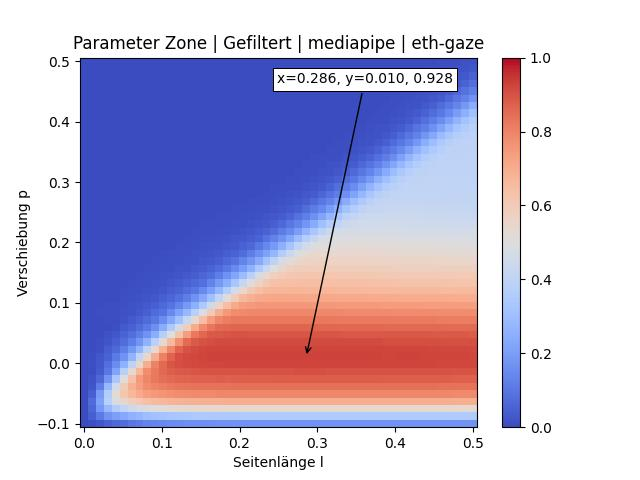
\includegraphics[width=\linewidth]{evaluation/mediapipe-eth-gaze-total-ignore-contour.jpg}
        \caption{Teilmenge der Videos}
        \label{fig:evaluation:threshold:mediapipe:eth-gaze:ignore}
    \end{subfigure}%
    \caption{Ergebnis des Hyperparameter-Tunings für die Gesichtserkennung mit \mediapipe und die Blickrichtungsbestimmung mit \ethg.}
    \label{fig:evaluation:threshold:mediapipe:eth-gaze}
\end{figure}
\begin{figure}{}
    \begin{subfigure}{0.45\textwidth}
        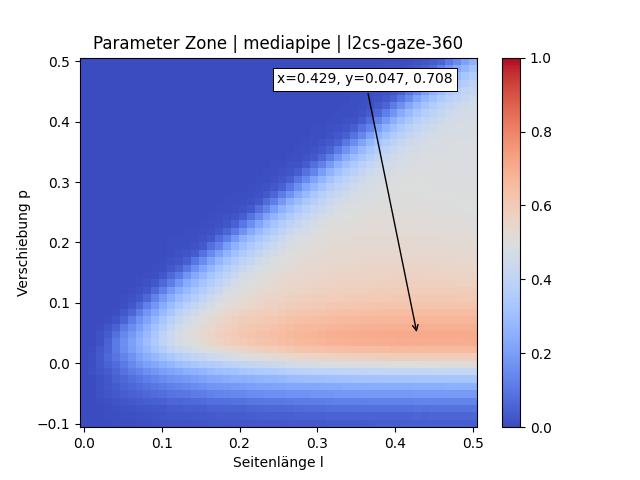
\includegraphics[width=\linewidth]{evaluation/mediapipe-l2cs-gaze-360-total-contour.jpg}
        \caption{Alle Videos}
        \label{fig:evaluation:threshold:mediapipe:l2cs-gaze-360:all}
    \end{subfigure}%
    \begin{subfigure}{0.45\textwidth}
        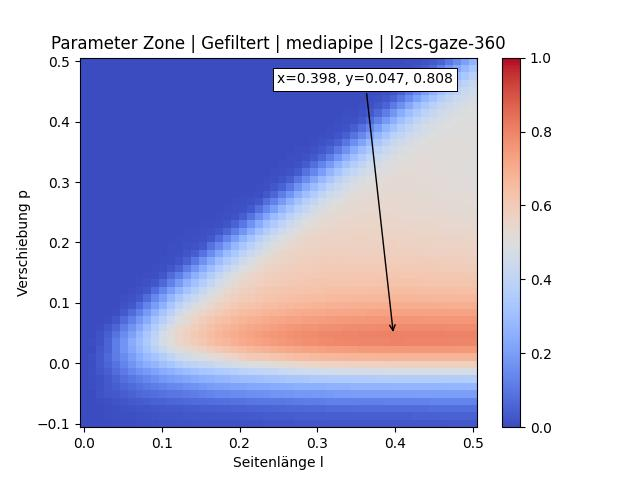
\includegraphics[width=\linewidth]{evaluation/mediapipe-l2cs-gaze-360-total-ignore-contour.jpg}
        \caption{Teilmenge der Videos}
        \label{fig:evaluation:threshold:mediapipe:l2cs-gaze-360:ignore}
    \end{subfigure}%
    \caption{Ergebnis des Hyperparameter-Tunings für die Gesichtserkennung mit \mediapipe und die Blickrichtungsbestimmung mit \gazed.}
    \label{fig:evaluation:threshold:mediapipe:l2cs-gaze-360}
\end{figure}
\begin{figure}{}
    \begin{subfigure}{0.45\textwidth}
        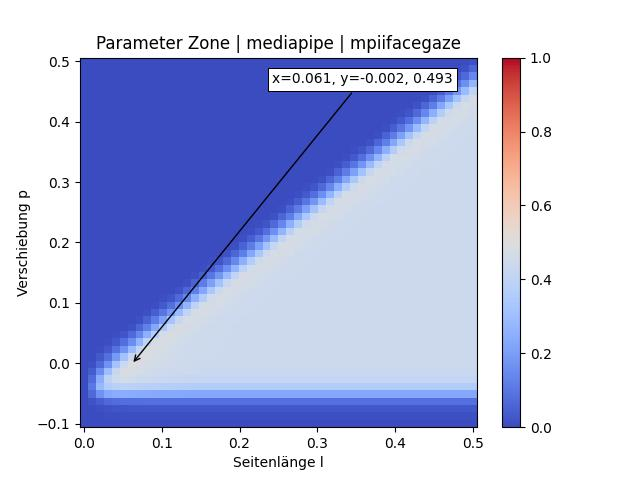
\includegraphics[width=\linewidth]{evaluation/mediapipe-mpiifacegaze-total-contour.jpg}
        \caption{Alle Videos}
        \label{fig:evaluation:threshold:mediapipe:mpiifacegaze:all}
    \end{subfigure}
    \begin{subfigure}{0.45\textwidth}
        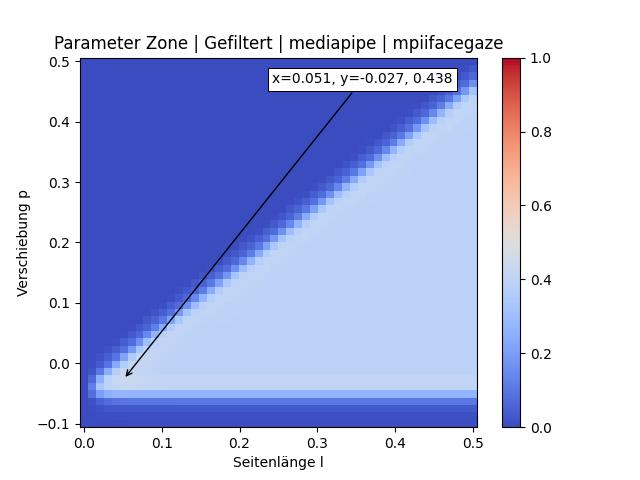
\includegraphics[width=\linewidth]{evaluation/mediapipe-mpiifacegaze-total-ignore-contour.jpg}
        \caption{Teilmenge der Videos}
        \label{fig:evaluation:threshold:mediapipe:mpiifacegaze:ignore}
    \end{subfigure}%
    \caption{Ergebnis des Hyperparameter-Tunings für die Gesichtserkennung mit \mediapipe und die Blickrichtungsbestimmung mit \mpii.}
    \label{fig:evaluation:threshold:mediapipe:mpiifacegaze}
\end{figure}
\begin{figure}{}
    \begin{subfigure}{0.45\textwidth}
        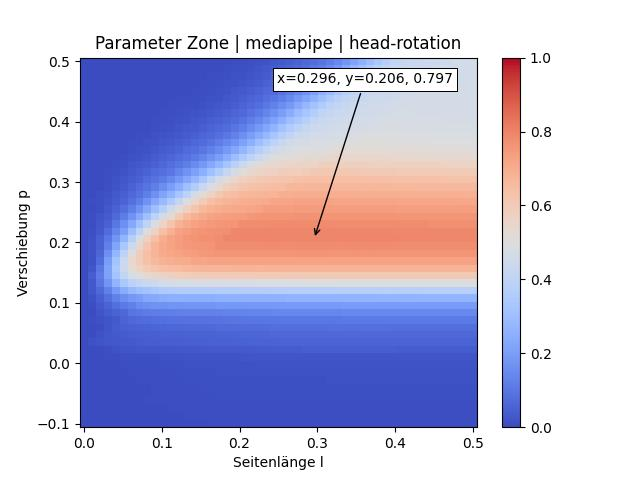
\includegraphics[width=\linewidth]{evaluation/mediapipe-head-rotation-total-contour.jpg}
        \caption{Alle Videos}
        \label{fig:evaluation:threshold:mediapipe:head-rotation:all}
    \end{subfigure}
    \begin{subfigure}{0.45\textwidth}
        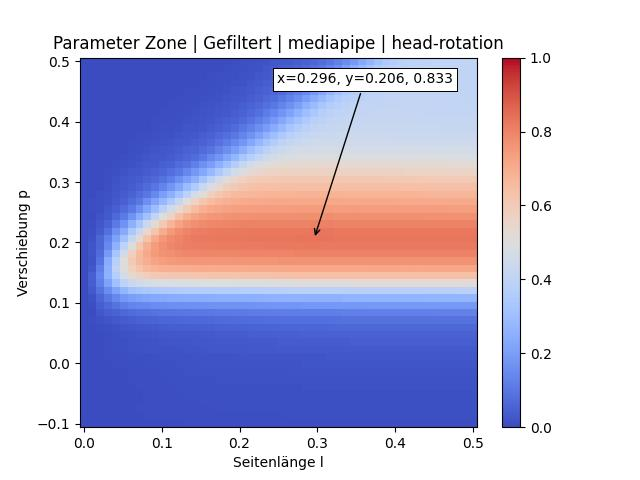
\includegraphics[width=\linewidth]{evaluation/mediapipe-head-rotation-total-ignore-contour.jpg}
        \caption{Teilmenge der Videos}
        \label{fig:evaluation:threshold:mediapipe:head-rotation:ignore}
    \end{subfigure}%
    \caption{Ergebnis des Hyperparameter-Tunings für die Gesichtserkennung mit \mediapipe und die Blickrichtungsbestimmung mittels der Kopfrotation.}
    \label{fig:evaluation:threshold:mediapipe:head-rotation}
\end{figure}

Betrachtet man die Diagramme in den Abbildungen \ref{fig:evaluation:threshold:dlib:eth-gaze} bis \ref{fig:evaluation:threshold:mediapipe:head-rotation} genauer, so scheint es, dass die Seitenlänge $\hitthresholdsize$ ab einem bestimmten Wert beliebig groß gewählt werden kann und dennoch ähnlich gute Ergebnissen erzielt werden. Bei der Vergrößerung von $\hitthresholdsize$ passiert vor allem, dass Schnittpunkte $\intersection$ von Personen, die links oder rechts neben das Smartphone schauen, als Blick auf das Smartphone interpretiert werden. Bereits in der Arbeit von Henseler \cite{bachelor:henseler:gaze-ebikes} konnte die Tendenz erkannt werden, dass, wenn Radfahrende ihren Blick vom Straßenverkehr abwenden, sie in fast allen Fällen auf das in der Halterung montierte Smartphone schauen. Von 1.516 Bildern schauten die Teilnehmenden der Studie von Henseler insgesamt nur vier Mal neben das Smartphone. Durch die scheinbar wirkungslose Vergrößerung der Seitenlänge $\hitthresholdsize$ ist diese Tendenz auch in den für diese Arbeit aufgenommenen Videos zu erkennen. Es ist daher zu beachten, dass je nach Wahl von $\hitthresholdsize$ Blicke links und rechts neben den Bildschirms nicht erkannt werden können. Dies wird unter anderem in Video 06 gezeigt. In diesem Video sitzt die dargestellte Person nicht auf dem Fahrrad, sondern ruht auf einer Bank. Dabei sieht die Person häufig links und rechts neben das Display des Smartphones. Die Ergebnisse des Hyperparameter-Tunings speziell für dieses Video sind in Abbildung \ref{fig:evaluation:threshold:daneben} dargestellt. Es ist zu erkennen, dass ab einer Seitenlänge von ca. 0,2 der F1-Score wieder abnimmt.

\begin{figure}
    \centering
    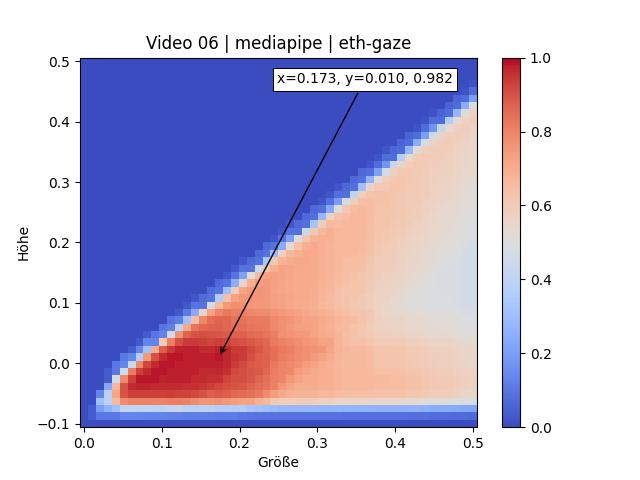
\includegraphics[width=0.6\linewidth]{evaluation/06-mediapipe-eth-gaze-contour.jpg}
    \caption{Ergebnisse des Hyperparameter-Tunings nur für Video 06.}
    \label{fig:evaluation:threshold:daneben}
\end{figure}

\subsubsection{Auswirkungen von Umwelteinflüssen auf die Blickrichtungsbestimmung}


Mittels der in Kapitel \ref{sec:evaluation:results:gaze:threshold} ermittelten Parameter $\hitthresholdsize$ und $\hitthresholdposition$ wurde für jedes Video der F1-Score berechnet, um die Leistungsfähigkeit der Ansätze unter verschiedenen Umgebungsbedingungen zu untersuchen. Es wurden die Parameter verwendet, die durch das Auslassen einiger Videos mit vermeidbaren Störfaktoren ermittelt wurden. Die Ergebnisse dieser Berechnung sind in Tabelle \ref{tab:evaluation:best:results} dargestellt. Im Anhang befindet sich eine detaillierte Auflistung der für den F1-Score erforderlichen Werte für alle Videos. 
\begin{table}[]
    \centering
    \begin{tabular}{c | c | c c c c}
    \toprule
        \textbf{Video} & \textbf{Gesichtsmodell} & \textbf{ETH-XGaze} & \textbf{Gaze360} & \textbf{MPIIFaceGaze} & \textbf{Kopfrotation} \\
        \hline
\multirow{2}{*}{01} & dlib & \cellcolor[HTML] {0DF200}\textcolor{black}{0,947} & \cellcolor[HTML] {10EE00}\textcolor{black}{0,93} & \cellcolor[HTML] {31CD00}\textcolor{black}{0,804} & \cellcolor[HTML] {3CC300}\textcolor{black}{0,765} \\ & MediaPipe & \cellcolor[HTML] {04FB00}\textcolor{black}{\textbf{0,983}} & \cellcolor[HTML] {34CB00}\textcolor{black}{0,794} & \cellcolor[HTML] {877800}\textcolor{white}{0,469} & \cellcolor[HTML] {28D700}\textcolor{black}{0,841} \\ \hline
\multirow{2}{*}{02} & dlib & \cellcolor[HTML] {0DF200}\textcolor{black}{\textbf{0,947}} & \cellcolor[HTML] {20DE00}\textcolor{black}{0,869} & \cellcolor[HTML] {45BA00}\textcolor{black}{0,73} & \cellcolor[HTML] {45BA00}\textcolor{black}{0,727} \\ & MediaPipe & \cellcolor[HTML] {0EF100}\textcolor{black}{0,943} & \cellcolor[HTML] {27D800}\textcolor{black}{0,846} & \cellcolor[HTML] {926D00}\textcolor{white}{0,429} & \cellcolor[HTML] {18E700}\textcolor{black}{0,903} \\ \hline
\multirow{2}{*}{03} & dlib & \cellcolor[HTML] {09F500}\textcolor{black}{0,959} & \cellcolor[HTML] {28D700}\textcolor{black}{0,843} & \cellcolor[HTML] {699500}\textcolor{black}{0,583} & \cellcolor[HTML] {48B700}\textcolor{black}{0,716} \\ & MediaPipe & \cellcolor[HTML] {06F900}\textcolor{black}{\textbf{0,973}} & \cellcolor[HTML] {718D00}\textcolor{white}{0,554} & \cellcolor[HTML] {C53A00}\textcolor{white}{0,227} & \cellcolor[HTML] {0EF100}\textcolor{black}{0,944} \\ \hline
\multirow{2}{*}{04} & dlib & \cellcolor[HTML] {0EF100}\textcolor{black}{\textbf{0,944}} & \cellcolor[HTML] {3BC300}\textcolor{black}{0,766} & \cellcolor[HTML] {7B8300}\textcolor{white}{0,518} & \cellcolor[HTML] {8F7000}\textcolor{white}{0,441} \\ & MediaPipe & \cellcolor[HTML] {0FF000}\textcolor{black}{0,938} & \cellcolor[HTML] {32CC00}\textcolor{black}{0,798} & \cellcolor[HTML] {986700}\textcolor{white}{0,405} & \cellcolor[HTML] {6C9300}\textcolor{black}{0,575} \\ \hline
\multirow{2}{*}{05} & dlib & \cellcolor[HTML] {10EF00}\textcolor{black}{0,936} & \cellcolor[HTML] {29D500}\textcolor{black}{0,834} & \cellcolor[HTML] {3FC000}\textcolor{black}{0,75} & \cellcolor[HTML] {38C700}\textcolor{black}{0,778} \\ & MediaPipe & \cellcolor[HTML] {01FD00}\textcolor{black}{\textbf{0,989}} & \cellcolor[HTML] {36C900}\textcolor{black}{0,786} & \cellcolor[HTML] {8D7100}\textcolor{white}{0,448} & \cellcolor[HTML] {27D800}\textcolor{black}{0,847} \\ \hline
\multirow{2}{*}{\textit{06}} & dlib & \cellcolor[HTML] {18E600}\textcolor{black}{\textbf{0,902}} & \cellcolor[HTML] {619E00}\textcolor{black}{0,62} & \cellcolor[HTML] {5FA000}\textcolor{black}{0,625} & \cellcolor[HTML] {807F00}\textcolor{white}{0,498} \\ & MediaPipe & \cellcolor[HTML] {38C600}\textcolor{black}{0,775} & \cellcolor[HTML] {4DB200}\textcolor{black}{0,697} & \cellcolor[HTML] {21DD00}\textcolor{black}{0,866} & \cellcolor[HTML] {7F8000}\textcolor{white}{0,5} \\ \hline
\multirow{2}{*}{\textit{07}} & dlib & \cellcolor[HTML] {A55900}\textcolor{white}{0,352} & \cellcolor[HTML] {A15E00}\textcolor{white}{0,368} & \cellcolor[HTML] {976800}\textcolor{white}{0,41} & \cellcolor[HTML] {A35C00}\textcolor{white}{0,363} \\ & MediaPipe & \cellcolor[HTML] {6C9300}\textcolor{black}{\textbf{0,574}} & \cellcolor[HTML] {AC5300}\textcolor{white}{0,325} & \cellcolor[HTML] {916E00}\textcolor{white}{0,431} & \cellcolor[HTML] {8C7300}\textcolor{white}{0,452} \\ \hline
\multirow{2}{*}{08} & dlib & \cellcolor[HTML] {4DB200}\textcolor{black}{\textbf{0,696}} & \cellcolor[HTML] {768900}\textcolor{white}{0,538} & \cellcolor[HTML] {E21D00}\textcolor{white}{0,115} & \cellcolor[HTML] {A95600}\textcolor{white}{0,337} \\ & MediaPipe & \cellcolor[HTML] {51AD00}\textcolor{black}{0,677} & \cellcolor[HTML] {51AE00}\textcolor{black}{0,681} & \cellcolor[HTML] {F50A00}\textcolor{white}{0,04} & \cellcolor[HTML] {728C00}\textcolor{white}{0,548} \\ \hline
\multirow{2}{*}{09} & dlib & \cellcolor[HTML] {17E800}\textcolor{black}{0,909} & \cellcolor[HTML] {0EF100}\textcolor{black}{0,942} & \cellcolor[HTML] {17E800}\textcolor{black}{0,908} & \cellcolor[HTML] {1FE000}\textcolor{black}{0,876} \\ & MediaPipe & \cellcolor[HTML] {2BD300}\textcolor{black}{0,829} & \cellcolor[HTML] {0BF300}\textcolor{black}{\textbf{0,955}} & \cellcolor[HTML] {46B900}\textcolor{black}{0,724} & \cellcolor[HTML] {1EE100}\textcolor{black}{0,881} \\ \hline
\multirow{2}{*}{\textit{10}} & dlib & \cellcolor[HTML] {59A500}\textcolor{black}{0,645} & \cellcolor[HTML] {837B00}\textcolor{white}{0,482} & \cellcolor[HTML] {936C00}\textcolor{white}{0,426} & \cellcolor[HTML] {1DE200}\textcolor{black}{0,886} \\ & MediaPipe & \cellcolor[HTML] {659A00}\textcolor{black}{0,604} & \cellcolor[HTML] {887700}\textcolor{white}{0,466} & \cellcolor[HTML] {817E00}\textcolor{white}{0,493} & \cellcolor[HTML] {10EF00}\textcolor{black}{\textbf{0,935}} \\ \hline
\multirow{2}{*}{11} & dlib & \cellcolor[HTML] {1EE100}\textcolor{black}{0,881} & \cellcolor[HTML] {28D700}\textcolor{black}{0,843} & \cellcolor[HTML] {48B700}\textcolor{black}{0,716} & \cellcolor[HTML] {46B900}\textcolor{black}{0,723} \\ & MediaPipe & \cellcolor[HTML] {0FF000}\textcolor{black}{\textbf{0,94}} & \cellcolor[HTML] {2ED100}\textcolor{black}{0,818} & \cellcolor[HTML] {9D6100}\textcolor{white}{0,386} & \cellcolor[HTML] {30CF00}\textcolor{black}{0,811} \\ \hline
\multirow{2}{*}{12} & dlib & \cellcolor[HTML] {0CF300}\textcolor{black}{0,951} & \cellcolor[HTML] {18E700}\textcolor{black}{0,906} & \cellcolor[HTML] {3DC200}\textcolor{black}{0,762} & \cellcolor[HTML] {3BC300}\textcolor{black}{0,768} \\ & MediaPipe & \cellcolor[HTML] {05FA00}\textcolor{black}{\textbf{0,978}} & \cellcolor[HTML] {37C800}\textcolor{black}{0,785} & \cellcolor[HTML] {AF5000}\textcolor{white}{0,313} & \cellcolor[HTML] {1CE300}\textcolor{black}{0,888} \\ \hline
\multirow{2}{*}{13} & dlib & \cellcolor[HTML] {12EC00}\textcolor{black}{0,922} & \cellcolor[HTML] {1DE200}\textcolor{black}{0,883} & \cellcolor[HTML] {2CD300}\textcolor{black}{0,826} & \cellcolor[HTML] {2BD300}\textcolor{black}{0,829} \\ & MediaPipe & \cellcolor[HTML] {0BF300}\textcolor{black}{\textbf{0,954}} & \cellcolor[HTML] {20DF00}\textcolor{black}{0,874} & \cellcolor[HTML] {897600}\textcolor{white}{0,461} & \cellcolor[HTML] {1DE200}\textcolor{black}{0,884} \\ \hline
\multirow{2}{*}{14} & dlib & \cellcolor[HTML] {3FC000}\textcolor{black}{0,754} & \cellcolor[HTML] {3FC000}\textcolor{black}{0,75} & \cellcolor[HTML] {4DB200}\textcolor{black}{0,698} & \cellcolor[HTML] {47B800}\textcolor{black}{0,719} \\ & MediaPipe & \cellcolor[HTML] {12EC00}\textcolor{black}{\textbf{0,925}} & \cellcolor[HTML] {47B800}\textcolor{black}{0,72} & \cellcolor[HTML] {9A6500}\textcolor{white}{0,396} & \cellcolor[HTML] {20DF00}\textcolor{black}{0,875} \\ \hline
\multirow{2}{*}{15} & dlib & \cellcolor[HTML] {02FC00}\textcolor{black}{\textbf{0,985}} & \cellcolor[HTML] {0EF100}\textcolor{black}{0,945} & \cellcolor[HTML] {1BE300}\textcolor{black}{0,891} & \cellcolor[HTML] {22DC00}\textcolor{black}{0,86} \\ & MediaPipe & \cellcolor[HTML] {02FC00}\textcolor{black}{\textbf{0,985}} & \cellcolor[HTML] {18E700}\textcolor{black}{0,905} & \cellcolor[HTML] {966900}\textcolor{white}{0,412} & \cellcolor[HTML] {0CF300}\textcolor{black}{0,953} \\ \hline
\multirow{2}{*}{16} & dlib & \cellcolor[HTML] {06F900}\textcolor{black}{\textbf{0,976}} & \cellcolor[HTML] {18E700}\textcolor{black}{0,905} & \cellcolor[HTML] {28D600}\textcolor{black}{0,837} & \cellcolor[HTML] {26D900}\textcolor{black}{0,851} \\ & MediaPipe & \cellcolor[HTML] {0CF300}\textcolor{black}{0,952} & \cellcolor[HTML] {11ED00}\textcolor{black}{0,927} & \cellcolor[HTML] {897600}\textcolor{white}{0,464} & \cellcolor[HTML] {0CF300}\textcolor{black}{0,952} \\ \hline
\multirow{2}{*}{17} & dlib & \cellcolor[HTML] {28D700}\textcolor{black}{0,843} & \cellcolor[HTML] {42BC00}\textcolor{black}{0,737} & \cellcolor[HTML] {29D500}\textcolor{black}{0,834} & \cellcolor[HTML] {30CE00}\textcolor{black}{0,807} \\ & MediaPipe & \cellcolor[HTML] {18E600}\textcolor{black}{\textbf{0,899}} & \cellcolor[HTML] {689700}\textcolor{black}{0,593} & \cellcolor[HTML] {32CC00}\textcolor{black}{0,799} & \cellcolor[HTML] {2FD000}\textcolor{black}{0,814} \\ \hline
\multirow{2}{*}{18} & dlib & \cellcolor[HTML] {18E700}\textcolor{black}{0,904} & \cellcolor[HTML] {20DE00}\textcolor{black}{0,868} & \cellcolor[HTML] {6D9200}\textcolor{black}{0,572} & \cellcolor[HTML] {56A900}\textcolor{black}{0,664} \\ & MediaPipe & \cellcolor[HTML] {14EB00}\textcolor{black}{\textbf{0,921}} & \cellcolor[HTML] {20DF00}\textcolor{black}{0,873} & \cellcolor[HTML] {B64900}\textcolor{white}{0,287} & \cellcolor[HTML] {20DE00}\textcolor{black}{0,871} \\ \hline
\multirow{2}{*}{19} & dlib & \cellcolor[HTML] {0BF300}\textcolor{black}{\textbf{0,956}} & \cellcolor[HTML] {10EF00}\textcolor{black}{0,935} & \cellcolor[HTML] {718D00}\textcolor{white}{0,552} & \cellcolor[HTML] {42BC00}\textcolor{black}{0,736} \\ & MediaPipe & \cellcolor[HTML] {0DF200}\textcolor{black}{0,946} & \cellcolor[HTML] {10EF00}\textcolor{black}{0,935} & \cellcolor[HTML] {936C00}\textcolor{white}{0,425} & \cellcolor[HTML] {27D800}\textcolor{black}{0,844} \\ \hline
\multirow{2}{*}{20} & dlib & \cellcolor[HTML] {10EE00}\textcolor{black}{0,932} & \cellcolor[HTML] {1DE200}\textcolor{black}{0,884} & \cellcolor[HTML] {35CA00}\textcolor{black}{0,79} & \cellcolor[HTML] {3CC300}\textcolor{black}{0,763} \\ & MediaPipe & \cellcolor[HTML] {10EE00}\textcolor{black}{\textbf{0,933}} & \cellcolor[HTML] {1EE100}\textcolor{black}{0,88} & \cellcolor[HTML] {699600}\textcolor{black}{0,588} & \cellcolor[HTML] {35CA00}\textcolor{black}{0,79} \\ \hline
\multirow{2}{*}{21} & dlib & \cellcolor[HTML] {0EF100}\textcolor{black}{0,945} & \cellcolor[HTML] {1CE300}\textcolor{black}{0,887} & \cellcolor[HTML] {32CC00}\textcolor{black}{0,799} & \cellcolor[HTML] {39C500}\textcolor{black}{0,772} \\ & MediaPipe & \cellcolor[HTML] {0EF100}\textcolor{black}{\textbf{0,945}} & \cellcolor[HTML] {2DD200}\textcolor{black}{0,821} & \cellcolor[HTML] {5DA200}\textcolor{black}{0,633} & \cellcolor[HTML] {38C600}\textcolor{black}{0,776} \\ \hline
\multirow{2}{*}{\textit{22}} & dlib & \cellcolor[HTML] {7D8200}\textcolor{white}{0,511} & \cellcolor[HTML] {FF0000}\textcolor{white}{0,0} & \cellcolor[HTML] {916E00}\textcolor{white}{0,43} & \cellcolor[HTML] {807F00}\textcolor{white}{0,498} \\ & MediaPipe & \cellcolor[HTML] {897600}\textcolor{white}{0,464} & \cellcolor[HTML] {FF0000}\textcolor{white}{0,0} & \cellcolor[HTML] {A35B00}\textcolor{white}{0,358} & \cellcolor[HTML] {689700}\textcolor{black}{\textbf{0,593}} \\ \hline
\multirow{2}{*}{\textit{23}} & dlib & \cellcolor[HTML] {42BC00}\textcolor{black}{0,737} & \cellcolor[HTML] {F30C00}\textcolor{white}{0,048} & \cellcolor[HTML] {8F7000}\textcolor{white}{0,439} & \cellcolor[HTML] {5DA200}\textcolor{black}{0,634} \\ & MediaPipe & \cellcolor[HTML] {2FD000}\textcolor{black}{0,816} & \cellcolor[HTML] {A55900}\textcolor{white}{0,353} & \cellcolor[HTML] {8F7000}\textcolor{white}{0,438} & \cellcolor[HTML] {2CD300}\textcolor{black}{\textbf{0,825}} \\ \hline
\multirow{2}{*}{\textit{24}} & dlib & \cellcolor[HTML] {25DA00}\textcolor{black}{\textbf{0,852}} & \cellcolor[HTML] {37C800}\textcolor{black}{0,782} & \cellcolor[HTML] {699500}\textcolor{black}{0,585} & \cellcolor[HTML] {2ED100}\textcolor{black}{0,817} \\ & MediaPipe & \cellcolor[HTML] {31CD00}\textcolor{black}{0,802} & \cellcolor[HTML] {6B9300}\textcolor{black}{0,58} & \cellcolor[HTML] {8E7100}\textcolor{white}{0,443} & \cellcolor[HTML] {2DD200}\textcolor{black}{0,822} \\ \hline

    \end{tabular}
    \caption{Übersicht über den F1-Score der einzelnen Videos in Abhängigkeit von $\hitthresholdsize$ und $\hitthresholdposition$. Aussortierte Videos sind kursiv dargestellt.}
    \label{tab:evaluation:best:results}
\end{table}

Mit \mpii wurden erwartungsgemäß keine guten Ergebnisse erzielt. Es ist jedoch zu erkennen, dass bis auf wenige Ausnahmen der F1-Score mit der Gesichtserkennung von \dlib deutlich besser ist als mit \mediapipe. Dies liegt, wie bereits erwähnt, daran, dass mit \mpii sehr viele \textit{False Positives} erkannt werden. Das liegt daran, dass Bilder ohne erkannte Gesichter als nicht auf das Smartphone schauend gewertet werden, und \dlib weniger Bilder erkennt als \mediapipe. So gibt es auch Videos, in denen die Blickrichtungsbestimmung mit \mpii sehr gut Ergebnisse erzielen konnte, wie zum Beispiel Video 09. Wie bereits im Kapitel \ref{sec:evaluation:results:face} erwähnt, ist \philipp in diesen Videos aus einem schwierigen Blickwinkel zu sehen, so dass nur Gesichter erkannt werden können, wenn die Person auf das Smartphone schaut.

Generell ist festzustellen, dass es Videos gibt, bei denen fast alle Methoden ein Problem haben. Dies sind vor allem die Videos mit vermeidbaren Störfaktoren (Videos 06, 07, 10, 22, 23 und 24). Diese schneiden schlechter ab, da sie bei der Berechnung der Parameter $\hitthresholdsize$ und $\hitthresholdposition$ nicht berücksichtigt wurden. Zusätzlich war der Grund, dass sie nicht beachtet wurden, dass mit diesen Störfaktoren generell weniger gute Ergebnisse erzielt werden konnten. Besonders schlecht schneiden Nacht-Videos 22, 23 und 24 ab. Dabei sind die Ergebnisse in Video 22 am schlechtesten. In den Videos 23 und 24, in denen die Beleuchtung stückweise besser wird, können auch bessere Ergebnisse erzielt werden. Besonders auffällig ist die schlechte Vorhersage von \gazed in Video 22. In diesem Video konnten keine \textit{True Positives} erkannt werden. Betrachtet man die Ergebnisse der Blickrichtungsbestimmung genauer, so fällt auf, dass der vorhergesagte Pitch- und Yaw-Winkel in diesen Fällen eine sehr große Abweichung von der tatsächlichen Blickrichtung aufweist, wie in Abbildung \ref{fig:evaluation:gaze:gaze360:error} zu sehen ist. Dies liegt daran, dass der \gazed Datensatz von Kellnhofer et al. \cite{paper:gaze360} keine Aufnahmen in dunkler Umgebung enthält. Auch wenn bei der Erstellung des Datensatzes Außenaufnahmen gemacht wurden, spiegeln diese nicht so dunkle Gesichter wider, wie sie in Video 22 zu sehen sind.



\begin{figure}
    \centering
    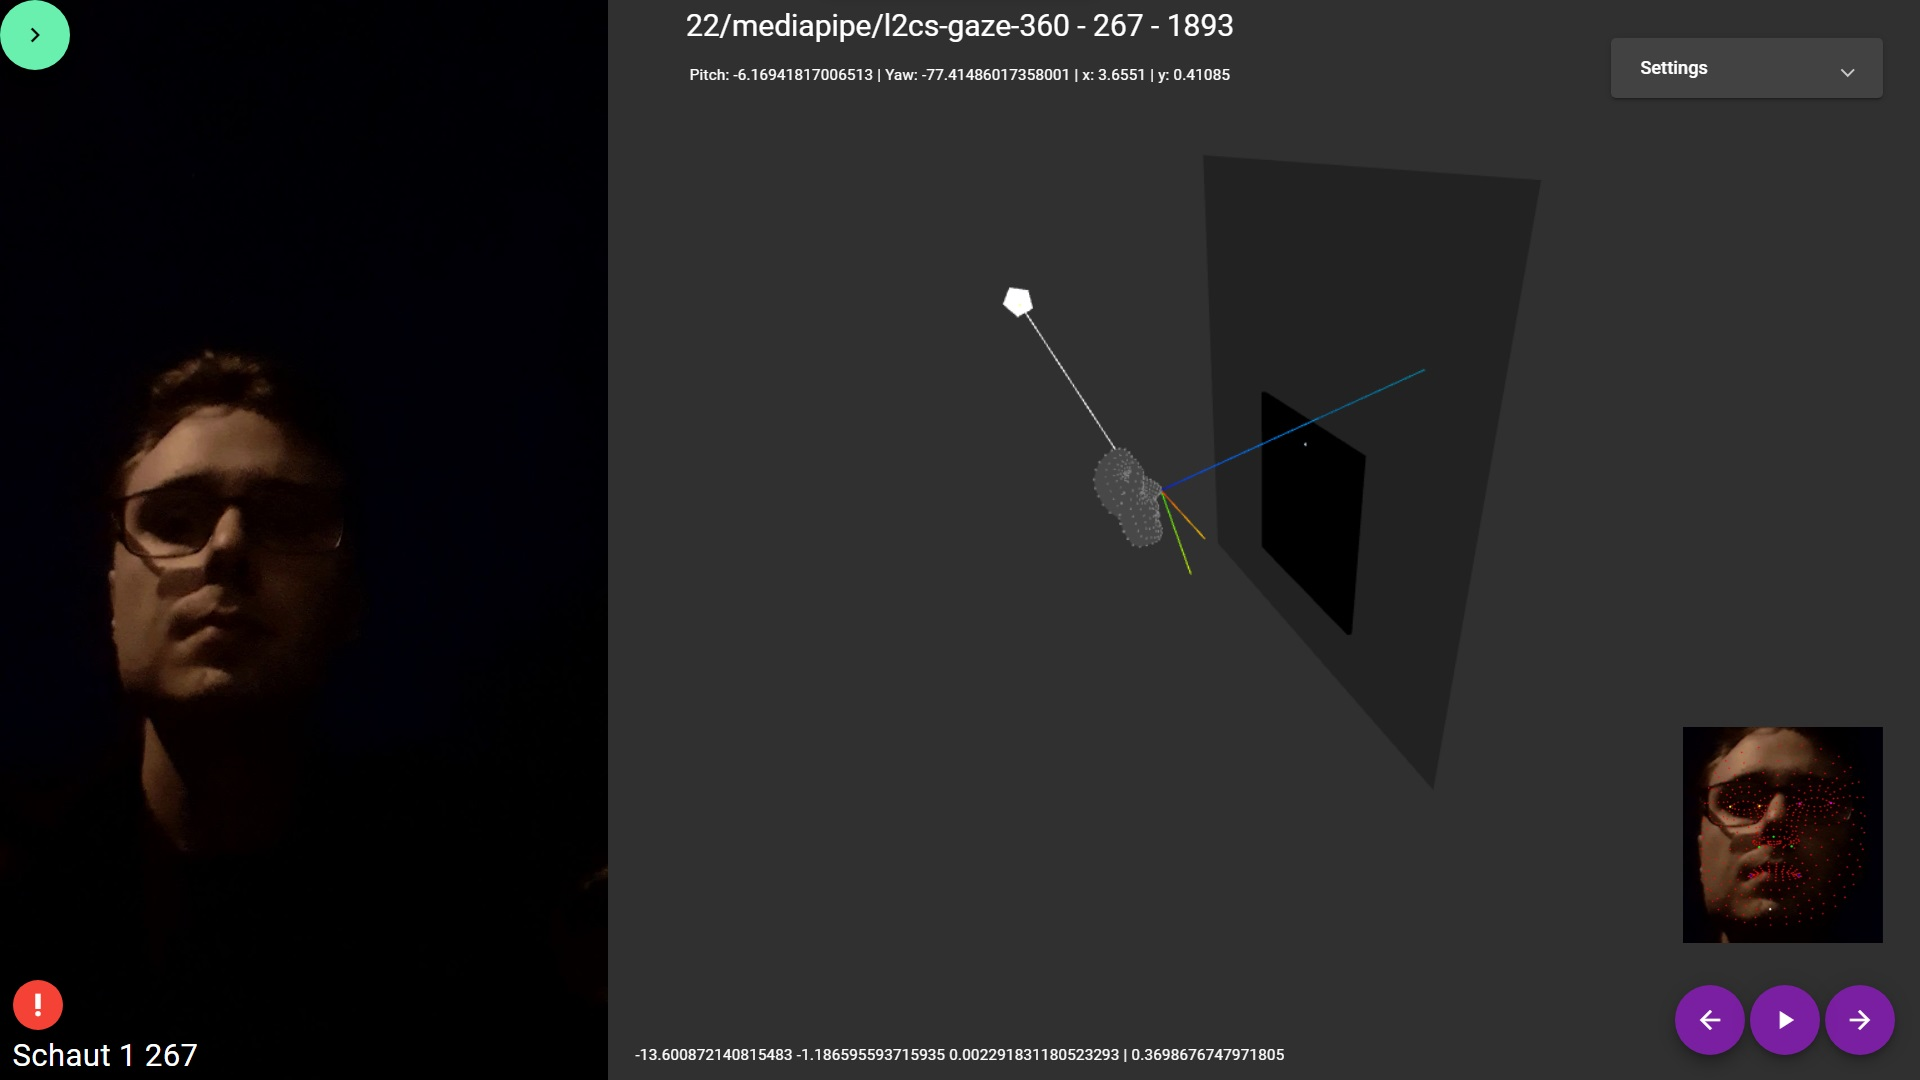
\includegraphics[width=0.9\linewidth]{evaluation/gaze360-error.jpg}
    \caption{Beispiel für die Blickrichtungsbestimmung mit \gazed bei Video 22. Es ist zu erkennen, dass der ermittelte Blickrichtungsvektor stark von der tatsächlichen Blickrichtung abweicht.}
    \label{fig:evaluation:gaze:gaze360:error}
\end{figure}

Weiterhin ist zu erkennen, dass die Verfahren zur Blickrichtungsbestimmung mit Convolutional Neural Networks in den Videos 07 und 10, in denen die dargestellten Personen eine Sonnenbrille tragen, Probleme haben.  Dagegen liefert die Blickrichtungsbestimmung mittels Kopfdrehung in Video 10 sehr gute Ergebnisse. Dies ist darauf zurückzuführen, dass die dargestellte Person in diesem Video, wie in Kapitel \ref{sec:evaluation:videos} beschrieben, den Kopf unnatürlich stark in Richtung des Smartphones neigt. In Video 07 hingegen kann auch mit der Kopfdrehung kein gutes Ergebnis erzielt werden. Dies ist jedoch auf das Auslassen der Videos bei der Bestimmung der Parameter zurückzuführen. Wie im Anhang in den Tabellen \ref{tab:appendix:07:local} (Video 07) und \ref{tab:appendix:10:local} (Video 10) zu sehen ist, werden bei der lokalen Berechnung der idealen Parameter mithilfe der Kopfdrehung jeweils die besten Ergebnisse mit einem F1-Score von 0,9 bzw. 0,977 erzielt.

Keine Auffälligkeiten zeigen hingegen die Videos, die durch Erschütterungen beeinträchtigt wurden (Video 04, 05, 12 und 13). Dies zeigt, dass Störfaktoren wie eine unebene Fahrbahnoberfläche von den Ansätzen gut kompensiert werden können. Auffällig ist auch, dass Video 14, das aufgrund der Sonne im Rücken der abgebildeten Person Probleme bei der Gesichtserkennung hatte, ebenfalls gute Ergebnisse erzielen konnte.

Es gibt jedoch ein Video, das keine besonderen Umgebungsbedingungen zeigt, für die Berechnung der Parameter verwendet wurde und dennoch schlechte Ergebnisse liefert. Es handelt sich um das Video 08 von \florian. Betrachtet man den bestmöglichen F1-Score, der bei der lokalen Berechnung der Parameter erzielt wurde (siehe Tabelle \ref{tab:appendix:08:local}), so fällt auf, dass dieser bei der Kombination von \mediapipe und \ethg mit 0,835 vergleichsweise niedrig ist. In allen anderen Videos, die keine Störfaktoren enthalten, liegt der F1-Score bei über 0,9. Daher wurde die Berechnung der lokalen Parameter des Videos genauer betrachtet. Dabei fiel auf, dass einige \textit{False Positives} in Momenten erkannt wurden, in denen \florian die Augen geschlossen hatte. Daher wurden die Bilder, in denen die Augen der Person geschlossen waren, aus der Betrachtung ausgeschlossen und die Parameterberechnung erneut durchgeführt. Wie in Abbildung \ref{fig:evaluation:threshold:mediapipe:eth-gaze:08} zu sehen ist, konnte der maximale F1-Score für das Video dadurch von 0,835 auf 0,944 verbessert werden. Dies zeigt, welchen Einfluss geschlossene Augen auf das Ergebnis haben können. Näheres dazu wird im folgenden Kapitel erläutert.

\begin{figure}{}
    \begin{subfigure}{0.45\textwidth}
        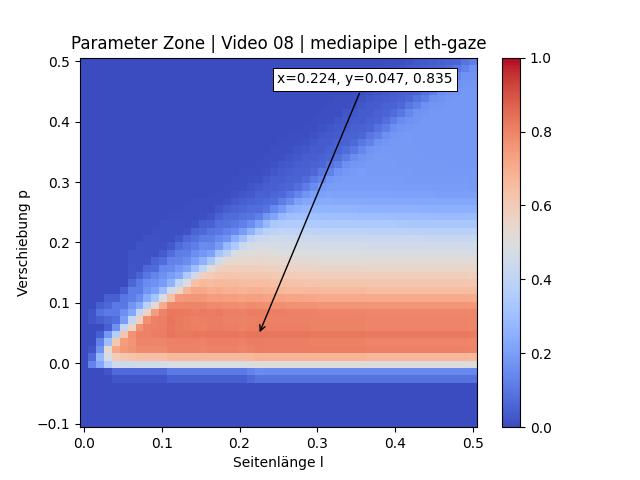
\includegraphics[width=\linewidth]{evaluation/08-mediapipe-eth-gaze-contour.jpg}
        \caption{Alle Bilder des Videos}
        \label{fig:evaluation:threshold:mediapipe:eth-gaze:08}
    \end{subfigure}
    \begin{subfigure}{0.45\textwidth}
        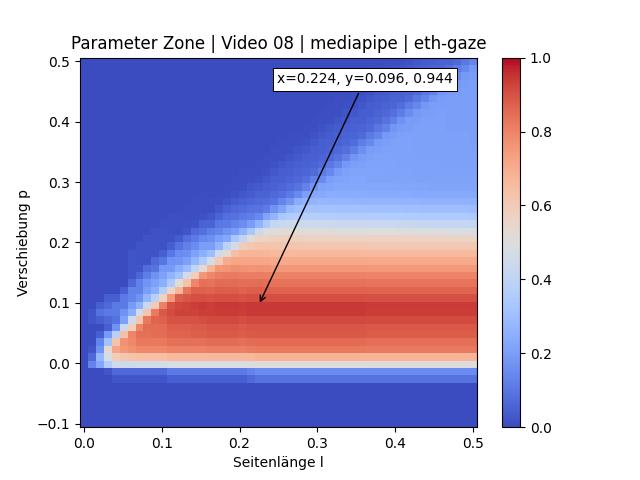
\includegraphics[width=\linewidth]{evaluation/08-mediapipe-eth-gaze-contour-without-blink.jpg}
        \caption{Nur Bilder mit geöffneten Augen}
        \label{fig:evaluation:threshold:mediapipe:eth-gaze:08:eye}
    \end{subfigure}%
    \caption{Ergebnis des Hyperparameter-Tunings basierend auf Video 08 mit Gesichtserkennung durch \mediapipe und Blickrichtungsbestimmung durch \ethg. Die Berechnung ist einmal mit allen Bildern des Videos in Abbildung \ref{fig:evaluation:threshold:mediapipe:eth-gaze:08} und einmal ohne Bilder, in denen die Augen der Person geschlossen waren, in Abbildung \ref{fig:evaluation:threshold:mediapipe:eth-gaze:08:eye} zu sehen.}
    \label{fig:evaluation:threshold:mediapipe:eth-gaze:08}
\end{figure}

\subsubsection{Auswirkung von geschlossenen Augen auf die Blickrichtungsbestimmung}\label{sec:evaluation:results:gaze:ear}

Teil des Konzepts der Blickrichtungsbestimmung mit Convolutional Neural Networks ist es, geschlossene Augen zu erkennen. Bilder mit geschlossenen Augen sollen, wie in Kapitel \ref{sec:concept:3d} beschrieben, bei der Bestimmung der Blickrichtung nicht beachtet werden. Im vorherigen Kapitel wurde bereits am Beispiel von Video 08 gezeigt, welchen Einfluss geschlossene Augen auf die Qualität der Blickrichtungsbestimmung haben können. Dies soll in diesem Kapitel weiter untersucht werden.

Als Grundlage wurde zunächst für jedes Bild untersucht, ob die Augen in diesem Bild geschlossen sind oder nicht, um eine Ground Truth zu erstellen. Im Kapitel \ref{tab:implementation:ear} wurde beschrieben, wie die Erkennung geschlossener Augen anhand der erkannten Gesichtsmerkmale um das Auge herum funktioniert. Dazu wird das \textit{Eye Aspect Ratio} \cite{paper:ear} für jedes erkannte Gesicht berechnet. Wie in Kapitel \ref{tab:implementation:ear} beschrieben, muss nun ein Grenzwert $\earthreshold$ bestimmt werden. Ist der $\ear$-Wert eines Gesichts kleiner als dieser Wert, werden die Augen als geschlossen betrachtet. 

Um den idealen Grenzwert zu bestimmen, wird der F1-Score verwendet. Die positiven Instanzen in diesem Fall sind alle Bilder mit geschlossenen Augen (Kategorie B.0). Die negativen Instanzen sind alle anderen Bilder. Anschließend wurde durch einen ersten Test ein Intervall ermittelt, in dem dieser Wert liegen muss:

\[
\earthreshold \in [0, 1]
\]

Dieses Intervall wird dann in 100 gleich große Schritte unterteilt. Jeder dieser Schritte wird als möglicher $\earthreshold$ angenommen, anhand dessen im Folgenden der F1-Score für jedes Video berechnet wird. Wie in Kapitel \ref{sec:evaluation:results:gaze:threshold}, wird auch diese Berechnung zweimal durchgeführt. Einmal mit allen Videos und einmal ohne die Videos mit vermeidbaren Störfaktoren wie Sonnenbrillen und dunkle Umgebungen bei Nacht. 

Die Ergebnisse sind in Tabelle \ref{tab:evaluation:ear} dargestellt. Es ist zu erkennen, dass mit diesem Ansatz geschlossene Augen nicht zuverlässig erkannt werden können. Der maximal erreichte F1-Score liegt bei 0,412. Gründe hierfür sind vor allem die schlechte Erkennung von Gesichtsmerkmalen um die Augen herum aufgrund der starken Kopfdrehung. Dadurch kann es vorkommen, dass die Gesichtspunkte ein geöffnetes Auge darstellen, obwohl das Auge in Wahrheit geschlossen ist. Außerdem wurde teilweise der Brillenrahmen als Auge erkannt, wie in Abbildung \ref{fig:evaluation:blink:false:positive} zu sehen ist, was zu einer falschen Erkennung eines geschlossenen Auges führt. Daher ist dieser Ansatz im Rahmen dieser Arbeit für die Erkennung geschlossener Augen nicht geeignet und wird daher für die weitere Auswertung nicht verwendet.

\begin{table}[]
    \centering
    \begin{tabular}{c | c c | c c}
        \toprule
        & \multicolumn{2}{c|}{\textbf{dlib}} &\multicolumn{2}{c}{\textbf{MediaPipe}} \\
        \midrule
        \textbf{Videos} & $\earthreshold$ & F1-Score & $\earthreshold$ & F1-Score \\
        \midrule
        Alle Videos & 0,183 & 0,325 & 0,165 & 0,362 \\
        Teilmenge der Videos & 0,173 & 0,362 & 0,159 & 0,412  \\
        \bottomrule
    \end{tabular}
    \caption{Maximaler mittlerer F1-Score für jede Methode mit Ausschluss der Bilder mit geschlossenen Augen im Vergleich zur Verarbeitung aller Bilder.}
    \label{tab:evaluation:ear}
\end{table}

\begin{figure}[]
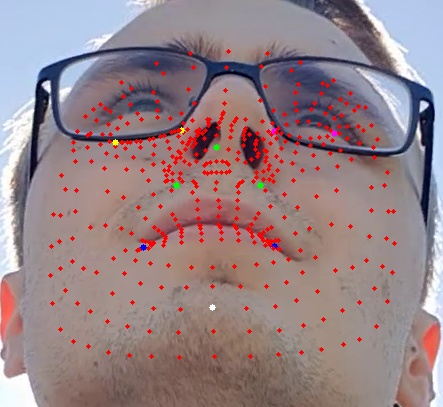
\includegraphics[width=0.5\linewidth]{evaluation/false_positive_blink.jpg}
\caption{Der Rahmen der Brille der Person wird als geschlossenes Auge erkannt.}\label{fig:evaluation:blink:false:positive}
\end{figure}

Da jedoch bereits in Video 08 gezeigt werden konnte, dass der F1-Score in diesem Video durch das Erkennen geschlossener Augen stark verbessert werden kann, soll untersucht werden, welche Verbesserung dadurch generell in den Videos erreicht werden kann. Dazu wurde das in Kapitel \ref{sec:evaluation:results:gaze:threshold} beschriebene Verfahren zur Bestimmung der idealen Parameter $\hitthresholdsize$ und $\hitthresholdposition$ erneut durchgeführt. Diesmal wurden jedoch die Bilder mit geschlossenen Augen anhand der Ground Truth erkannt und bei der Berechnung ignoriert. Die Ergebnisse sind in Tabelle \ref{tab:evaluation:blinks:filtered} dargestellt. Es ist zu erkennen, dass in allen Fällen der F1-Score durch das Erkennen der Augen verbessert werden konnte.

\begin{table}[]
\begin{tabular}{p{4cm} l c c c c}
\toprule
              &  & \textbf{ETH-XGaze} &\textbf{Gaze360}  & \textbf{MPIIFaceGaze} & \textbf{Kopfrotation} \\
\midrule
\multirowcell{2}{Teilmenge\\der Videos} & dlib          & 0,91            & 0,848    & 0,704  & 0,729            \\
                                        & MediaPipe    & 0,928    & 0,808                  & 0,439& 0,833          \\

\midrule
\multirowcell{2}{Teilmenge Videos ohne \\  geschlossene Augen} & dlib           & 0,920             & \textbf{0,855}          & \textbf{0,715} & 0,745                     \\
                                                            & MediaPipe      & \textbf{0,942}    & 0,817           & 0,450  & \textbf{0,846} \\               
\bottomrule
\caption{Darstellung der maximalen F1-Scores beim Aussortieren von Bildern mit geschlossen Augen. Zum Vergleich werden die F1-Scores aus Tabelle \ref{tab:evaluation:results:gaze:best:f1} gezeigt.}
\label{tab:evaluation:blinks:filtered}
\end{tabular}
\end{table}


\section{Zusammenfassung}

In diesem Kapitel wurde gezeigt, wie die Evaluation der erarbeiteten Konzepte durchgeführt wurde. Dazu wurden Videos von Radfahrenden in verschiedenen Situationen aufgenommen. Die Teilnehmenden wurden über das Ziel des Experiments informiert, was ihr Blickverhalten beeinflusst haben könnte. Die meisten Videos wurden von einer Person aufgenommen.

Zunächst wurde untersucht, wie gut die Gesichert der Radfahrenden mit \mediapipe und \dlib   erkannt werden können. Dabei zeigte sich, dass \mediapipe in deutlich mehr Bildern ein Gesicht erkennen konnte. Allerdings konnte auch mit \mediapipe in 9.546 von insgesamt 22.339 Bildern kein Gesicht erkannt werden. Es wurde jedoch gezeigt, dass in fast allen Fällen, in denen die Radfahrenden auf das Smartphone schauten, ein Gesicht erkannt werden konnte. Daraus kann geschlossen werden, dass wenn kein Gesicht erkannt wurde, die Person zu diesem Zeitpunkt nicht auf das Smartphone geschaut hat.

Als generelle Probleme bei der Gesichtserkennung konnten die Drehung des Kopfes, insbesondere entlang der Querachse, identifiziert werden. Weiterhin wurde festgestellt, dass extreme Lichtverhältnisse, z.B. bei Nacht, die Gesichtserkennung verschlechtern. 

Anschließend wurde die Blickrichtungsbestimmung ausgewertet. Dazu wurden für die Videos zunächst die Parameter $\hitthresholdsize$ und $\hitthresholdposition$ anhand der Ground Truth des Blickkontaktes bestimmt.  Dabei ist zu beachten, dass in den Videos zur Berechnung dieser Parameter hauptsächlich \markus zu sehen war. Die besten Ergebnisse wurden bei der Blickrichtungsbestimmung mit \ethg erzielt. Basierend auf der Gesichtserkennung von \mediapipe konnte ein F1-Score von 0,928 erreicht werden, bei \dlib waren es 0,91. Aber auch mit \gazed (0,848) und der Blickrichtungsbestimmung anhand der Kopfdrehung (0,833) konnten gute Ergebnisse erzielt werden. Weiterhin wurde gezeigt, dass der \mpii-Datensatz \cite{paper:mpiifacegaze} nicht für die Bestimmung der Blickrichtung von Radfahrern geeignet ist. Bei der Berechnung der Parameter wurde davon ausgegangen, dass keine im Rahmen der Studie beeinflussbaren Störfaktoren (Sonnenbrille, Tageszeit) in den Videos vorhanden sind.

Schließlich wurde der Einfluss geschlossener Augen auf die Ergebnisse untersucht. Es konnte festgestellt werden, dass die Erkennung geschlossener Augen die Ergebnisse aller Methoden zur Bestimmung der Blickrichtung verbessert. Der in dieser Arbeit implementierte Ansatz zur Erkennung geschlossener Augen lieferte jedoch nur sehr ungenaue Ergebnisse. Daher wurde dieser Ansatz für die weitere Auswertung nicht verwendet.













  \chapter{Fazit}\label{sec:fazit}

\section{Ergebnisse}

In dieser Arbeit wurden verschiedene Methoden zur Bestimmung der Blickrichtung von Radfahrenden anhand des Videostreams der Innenkamera eines Smartphones vorgestellt. Anhand dieser Blickrichtung wurde untersucht, wie gut man messen kann, zu welchen Zeitpunkten die Radfahrenden auf das Display ihres Smartphones sehen.

\vspace{0.3cm}
\noindent\textbf{Forschungsfrage 1} \textit{Was ist die beste Möglichkeit, nur mittels der Frontkamera eines mobilen Geräts die Blickrichtung der Nutzenden während der Fahrt zu verfolgen?}
\vspace{0.3cm}

In dieser Arbeit wurden verschiedene Möglichkeiten zur Bestimmung der Blickrichtung vorgestellt.

Zuerst wurde untersucht, ob Deep Learning Appearance-Based Methoden, die Bildschirmkoordinaten vorhersagen können, für die Blickrichtungsbestimmung von Radfahrenden geeignet sind. Dabei wurde festgestellt, dass solche Modelle nicht in der Lage sind zu unterscheiden, ob eine Person auf den Bildschirm schaut oder nicht.

Es wurden zwei Konzepte entwickelt. In beiden Konzepten wird zunächst das Gesicht einer Person im Bild erkannt. Dazu werden \mediapipe und \dlib verwendet. Anschließend wird die dreidimensionale Blickrichtung der Person anhand der Kopfdrehung der dargestellten Person und mithilfe von drei verschiedenen Convolutional Neural Networks bestimmt. Für das Training der Modelle werden die Datensätze \ethg \cite{paper:eth-xgaze}, \gazed \cite{paper:gaze360} und \mpii \cite{paper:mpiifacegaze} verwendet.

Die Auswertung ergab, dass die besten Ergebnisse mit der Kombination von \mediapipe und \ethg erzielt wurden. Mit dieser Kombination wurde ein F1-Score von 0,928 erreicht. Mit der Kombination von \dlib und \ethg wurde ein F1-Score von 0,91 erreicht. Somit sind Deep Learning Appearance-Based Methoden auf Basis des \textit{ETH-XGaze} Datensatz am besten geeignet, um die Blickrichtung von Radfahrenden zu bestimmen. Für die Gesichtserkennung ist die Empfehlung, \mediapipe zu verwenden. 

Es ist jedoch anzumerken, dass auch das Konzept zur Bestimmung der Blickrichtung anhand der Kopfdrehung gute Ergebnisse erzielte (F1-Score von 0,833).

\vspace{0.3cm}
\noindent\textbf{Forschungsfrage 2} \textit{Wie präzise lässt sich mit der Frontkamera eines Smartphones, welches am Lenker eines Fahrrads befestigt ist, bestimmen, zu welchen Zeitpunkten eine Person während der Fahrt auf das Smartphone sieht?}
\vspace{0.3cm}

Für die Interpretation der Blickrichtung des Radfahrenden wird eine Ebene $\cameraplane$ definiert, auf der sich sowohl die Kamera als auch das Display des Smartphones befinden. Das Display des Smartphones wird dabei durch eine Zone modelliert, die durch eine Seitenlänge $\hitthresholdsize$ und einen Versatz $\hitthresholdposition$ beschrieben werden kann. Aus der dreidimensionalen Position des Kopfes relativ zur Kamera und dem ermittelten Blickrichtungsvektor wird eine Gerade konstruiert, die die Ebene $\cameraplane$ im Punkt $\intersection$ schneidet. Liegt dieser Schnittpunkt innerhalb des vom Smartphone repräsentierten Bereichs, so wird angenommen, dass die Person auf das Smartphone schaut. 

Während der Evaluation wurden die idealen Parameter $\hitthresholdsize$ und $\hitthresholdposition$ anhand der aufgezeichneten Videos ermittelt. Mit diesen Parametern konnte mit der Blickrichtungsbestimmung mit \ethg und der Gesichtserkennung mit \mediapipe ein F1-Score von 0,928 erreicht werden. Kalibriert man die Werte für jedes Video einzeln, können fast perfekte Werte erzielt werden. Eine genaue Auflistung dieser Werte für die einzelnen Videos ist im Anhang der Arbeit zu finden.

\vspace{0.3cm}
\noindent\textbf{Forschungsfrage 3} \textit{Welche technischen Hürden sind zu überwinden, um eine Blickrichtungserkennung mittels Smartphones auf einem Fahrrad zu entwickeln?}
\vspace{0.3cm}

Für die derzeitige Umsetzung der Konzepte müssen Videos von Radfahrenden während der Fahrt aufgenommen werden. Für jedes Bild des Videos muss dann ein Gesicht sowie die dreidimensionale Position des Gesichts relativ zur Kamera bestimmt werden. Für die Erkennung von Gesichtern und Gesichtsmerkmalen werden Algorithmen verwendet, die für den Einsatz auf Smartphones optimiert sind. Um auf die dreidimensionale Position des Kopfes zu schließen, wurde das \textit{Pose Computation Problem} \cite{paper:pose:problem} gelöst. Zur genauen Bestimmung dieser Position werden die im Kapitel \ref{sec:implementation:face:3d} vorgestellten intrinsischen Kameraparameter benötigt. Da diese für jede verwendete Kamera durch einen Kalibrierungsprozess ermittelt werden müssen, wurden sie im Rahmen dieser Arbeit geschätzt. Dabei ist zu beachten, dass durch die Schätzung der Kameraparameter die Ergebnisse nicht so genau sind wie mit ermittelten Kameraparametern. Mithilfe der intrinsischen Kameraparameter und eines dreidimensionalen Template-Modells eines Kopfes wurden dann ein Rotations- und ein Translationsvektor bestimmt, die zur Berechnung der dreidimensionalen Position jedes erkannten Gesichts verwendet werden können. 
Im nächsten Schritt wurde eine Blickrichtungsbestimmung mit den beiden vorgestellten Konzepten auf Basis der erkannten Gesichter implementiert. Wie bereits erwähnt, musste für die Interpretation der so ermittelten Blickrichtung ein idealer Bereich auf der Ebene $\cameraplane$ gefunden werden. Dazu wurde ein Hyperparameter-Tuning durchgeführt.

\vspace{0.3cm}
\noindent\textbf{Forschungsfrage 4} \textit{Wie kann die Qualität der aufgezeichneten Daten maximiert und Fehler minimiert werden?}
\vspace{0.3cm}

Um die Qualität der Daten zu maximieren, wurde zunächst experimentiert, mit welchen Konfigurationen der Gesichtserkennungsmethoden eine robuste Gesichtserkennung möglich ist. Eine genaue Evaluierung dieser Konfigurationen konnte im Rahmen dieser Arbeit nicht durchgeführt werden, da die Qualitätsbewertung ein sehr zeitaufwändiger Prozess ist.

Weiterhin wurde untersucht, ob eine Aussage darüber getroffen werden kann, ob die Person auf ihr Smartphone schaut, wenn kein Gesicht erkannt wurde. Es konnte gezeigt werden, dass in solchen Fällen fast ausschließlich nicht auf das Smartphone geschaut wird. Somit kann auch für Lücken in der Gesichtserkennung eine Aussage getroffen werden.

Bei näherer Betrachtung der mit \dlib erkannten Gesichter wurde deutlich, dass mit dieser Methode aufgrund der gemessenen Distanz zwischen dem Kopf des Radfahrenden und der Kamera schlecht erkannte Gesichter detektiert werden können. Die Datenqualität konnte durch das Aussortieren dieser Gesichter weiter verbessert werden.

Außerdem wurde festgestellt, dass Sonnenbrillen und Nachtfahrten die Gesichtserkennung erheblich beeinträchtigen. Um optimale Ergebnisse während einer Studie zu erzielen, sollte daher auf das Tragen von Sonnenbrillen während der Fahrt verzichtet werden. Außerdem sollten Nachtfahrten vermieden werden.

Die Auswertung zeigte auch, dass die Erkennung geschlossener Augen die Ergebnisse der Blickrichtungsbestimmung verbessern kann. Leider konnte der in dieser Arbeit verwendete Ansatz zur Erkennung geschlossener Augen diese Bilder nicht zuverlässig erkennen.

\vspace{0.3cm}
\noindent\textbf{Forschungsfrage 5} \textit{
Wie gut können die genannten Umwelteinflüsse (Licht, Erschütterungen) kompensiert werden?}
\vspace{0.3cm}

Für die Auswertung der Arbeit wurden Videos von Radfahrern in verschiedenen Situationen aufgenommen. Bei der Auswertung der Gesichtserkennung wurde vor allem eine starke Kopfdrehung als Ursache für nicht erkannte Gesichter identifiziert. Normale Umwelteinflüsse konnten bei der Gesichtserkennung gut kompensiert werden. Die Umgebungsbedingungen wurden nur in extremen Fällen zum Problem. So konnten bei Nachtaufnahmen sowie bei Aufnahmen, bei denen die Sonne im Rücken der Radfahrenden stand, keine Gesichter erkannt werden. Erschütterungen, die die Qualität der Videos beeinträchtigten, konnten ohne weitere Auffälligkeiten verarbeitet werden.

Bei der anschließenden Blickrichtungsbestimmung konnten die Umwelteinflüsse in der Regel gut kompensiert werden. Auch hier gab es keine Auffälligkeiten bei den Videos mit Erschütterungen und normalen Umwelteinflüssen. Da die Blickrichtungsbestimmung auf den Ergebnissen der Gesichtserkennung aufbaut, wurden bei den Nachtvideos schlechtere Ergebnisse erzielt. Für das Video, in dem die Sonne direkt im Rücken der Person zu sehen ist (Video 14), konnte trotz fehlender Gesichtserkennung mit der Kombination aus \mediapipe und \ethg ein F1-Score von 0,925 erreicht werden.

Zusammenfassend kann gesagt werden, dass normale Umwelteinflüsse durch die Implementierung kompensiert werden können.

\vspace{0.3cm}
\noindent\textbf{Forschungsfrage 6} \textit{Wie gut lässt sich die Messung durchführen, wenn Teile des Gesichts der Person verdeckt sind?}
\vspace{0.3cm}

Die Evaluation hat gezeigt, dass Sonnenbrillen für die Blickrichtungsbestimmung mit Convolutional Neural Networks nicht geeignet sind. Mit dem Konzept der Blickrichtungsbestimmung durch Kopfdrehung konnten jedoch auch mit Sonnenbrillen gute Ergebnisse erzielt werden. Dennoch ist es ratsam, im Rahmen einer Studie auf Sonnenbrillen zu verzichten. Das Tragen einer normalen Brille beeinträchtigte die Ergebnisse der Blickrichtungsbestimmung nicht. Es traten jedoch teilweise Probleme bei der Gesichtserkennung auf, da der Brillenrahmen als Auge erkannt wurde. Dadurch wurde die zuverlässige Erkennung geschlossener Augen beeinträchtigt.

\vspace{0.3cm}
\noindent\textbf{Forschungsfrage 7} \textit{Welche Kalibrierungen müssen zwingend vorgenommen werden, damit das Eye-Tracking funktioniert?}
\vspace{0.3cm}

Wie bereits erwähnt, ist es notwendig, für eine ideale Bestimmung der dreidimensionalen Position des Kopfes relativ zur Kamera, die intrinsischen Kameraparameter zu bestimmen. Diese können mit einer Kalibrierung präzise bestimmt werden. Im Rahmen dieser Arbeit wurden jedoch auch mit geschätzen Kameraparametern gute Ergebnisse erzielt.

Die Ergebnisse basieren auf den Parametern $\hitthresholdsize$ und $\hitthresholdposition$, die im Rahmen dieser Arbeit kalibriert wurden. Diese Parameter wurden hauptsächlich anhand von Videos einer einzelnen Person bestimmt. Daher können die Parameter durch das Aussehen dieser Person beeinflusst worden sein, auch wenn versucht wurde, möglichst viele verschiedene Blickwinkel auf die Person zu zeigen. Im Rahmen dieser Arbeit konnten jedoch auch mit Videos anderer Personen gute Ergebnisse erzielt werden. Generell sollte jedoch darauf geachtet werden, dass die Person im Blickwinkel der Innenkamera des Smartphones gut zu sehen ist.  


\section{Ausblick}

Mit den Ergebnissen dieser Arbeit kann in zukünftigen Studien im Rahmen der PrioBike-App gemessen werden, zu welchen Zeitpunkten eine Person auf das Smartphone schaut. Damit können unter anderem die in der Arbeit von Pickhardt \cite{diplom:paul:pickhardt} vorgestellten multimodalen Interaktionskonzepte der App evaluiert werden. Darüber hinaus können durch die Analyse des Blickverhaltens der Radfahrenden potentiell ablenkende Ansichten in der App identifiziert werden. Insgesamt kann mit dieser Arbeit ein wichtiger Beitrag zur sicheren Nutzung der PrioBike-App geleistet werden.

Im Rahmen dieser Arbeit konnte gezeigt werden, dass die Ergebnisse der Blickrichtungsbestimmung verbessert werden können, wenn Bilder mit geschlossenen Augen bei der Betrachtung ausgeschlossen werden. Ein möglicher Ansatz zur Erkennung geschlossener Augen wurde vorgestellt, konnte jedoch keine zuverlässigen Ergebnisse liefern. Zur Optimierung des Verfahrens könnten daher weitere Untersuchungen durchgeführt werden, wie eine robuste Erkennung geschlossener Augen ermöglicht werden kann.

In dieser Arbeit wurden hauptsächlich Gesichtserkennungsmethoden verwendet, die für den Einsatz auf mobilen Geräten optimiert wurden. Weitere Methoden konnten im zeitlichen Rahmen dieser Arbeit nicht getestet werden. Die Evaluation hat gezeigt, dass die verwendeten Verfahren Schwierigkeiten haben, ein Gesicht bei einer hohen Rotation des Kopfes um die Querachse zu erkennen. Die allgemeinen Ergebnisse der Erkennung von Blicken auf das Smartphone-Display wurden dadurch nicht beeinträchtigt. Dennoch könnten andere Methoden zur Gesichtserkennung untersucht werden, wie sie unter anderem von Khabarlak et al. in ihrer Arbeit \cite{paper:face:survey} vorgestellt wurden. 

Weiter konnte gezeigt werden, dass die Kalibrierung der Zone für ein einzelnes Video nahezu perfekte Ergebnisse für dieses Video ermöglicht hat. Im Rahmen dieser Arbeit wurde nicht untersucht, ob es möglich ist, vor Fahrtbeginn diese Zone speziell für eine Person zu kalibrieren. Wenn eine solche Methode gefunden werden kann, könnte dadurch die Qualität der Vorhersage weiter verbessert werden.

Im Rahmen dieser Arbeit wurde die Erkennung von zweidimensionalen Bildschirmkoordinaten nicht weiter verfolgt, da mit diesen Ansätzen nicht unterschieden werden kann, ob die Person auf das Smartphone schaut oder nicht. Da in dieser Arbeit jedoch ein Verfahren vorgestellt wurde, mit dem Blicke auf das Smartphone detektiert werden können, könnte in diesen Fällen ein solches Modell verwendet werden, um genauer zu untersuchen, auf welchen Bereich des Displays eine Person schaut.

Während einer Fahrt mit der PrioBike-App werden noch viele weitere Daten gesammelt, z.B. über die Geschwindigkeit und die gefahrene Strecke. Diese Daten könnten genutzt werden, um das Konzept zu erweitern, indem z.B. je nach Anwendungsfall Passagen ignoriert werden, in denen die Person nicht fährt, sondern steht.






  \newpage
  \cleardoublepage
  

  % use lowercased roman page numbers for the appendix and the bibliography
  \pagenumbering{roman}
  \newpage

  \printbibliography[heading=bibintoc]\label{sec:bibliography}%
  
   \cleardoublepage
  \begin{appendices}
    \tocless\chapter{Auswertung Videos}\label{appendix:a}
\section{Video 01}
\begin{figure}[H]
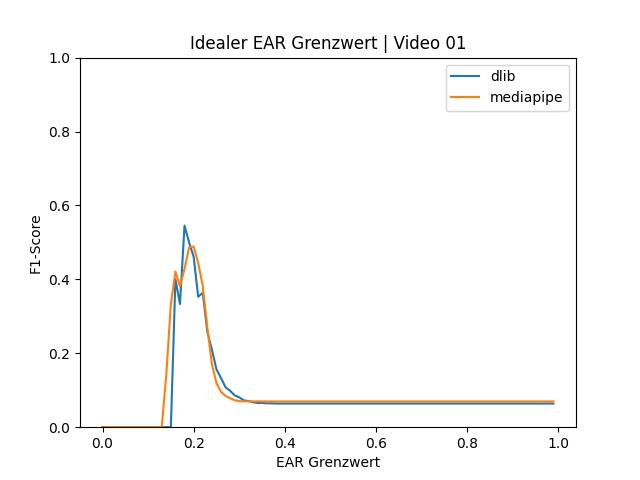
\includegraphics[width=0.7\linewidth]{appendix/01_f1-score-blink.jpg}
\caption{Ergebnisse der Bestimmung des idealen EAR-Grenzwerts für Video 01.}
\end{figure}

\begin{figure}[H]
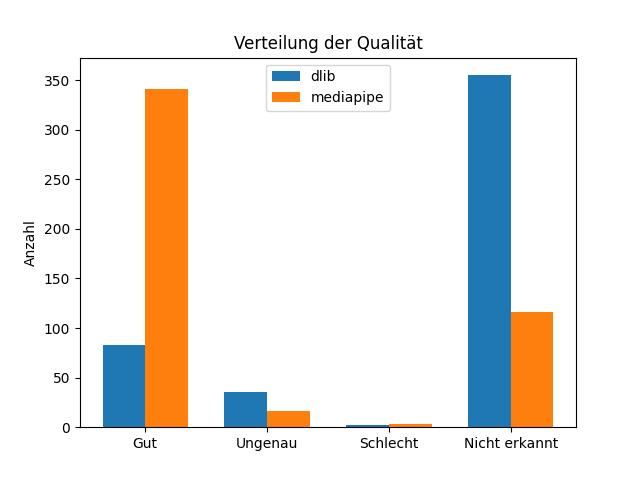
\includegraphics[width=0.7\linewidth]{appendix/01_bar-quality.jpg}
\caption{Aufteilung der Gesichtserkennungsqualität von Video 01.}
\end{figure}

\begin{table}[H]
\centering
\begin{tabular}{l|l|c c |c}
\toprule
\textbf{Gesichtserkennung} & \textbf{Blickrichtung} & \textbf{Seitenlänge} $\hitthresholdsize$ & \textbf{Verschiebung} $\hitthresholdposition$ & \textbf{F1-Score} \\ 
\midrule
\multirow{4}*{dlib}& ETH-XGaze & 0,133 & 0,01 & 0,952  \\ 
& Gaze360 & 0,296 & 0,035 & 0,952 \\ 
& MPIIFaceGaze & 0,041 & -0,039 & 0,826  \\ 
& Kopfrotation & 0,235 & 0,218 & 0,786  \\ 
\hline\multirow{4}*{MediaPipe}& ETH-XGaze & 0,122 & -0,002 & 0,983  \\ 
& Gaze360 & 0,265 & 0,035 & 0,872 \\ 
& MPIIFaceGaze & 0,031 & -0,039 & 0,57  \\ 
& Kopfrotation & 0,194 & 0,218 & 0,863  \\ 
\bottomrule\end{tabular}
\caption{Ergebnis des Hyperparameter-Tunings für die Zone speziell für Video 01.}
\label{tab:appendix:01:local}
\end{table}
\begin{table}[H]
\centering
\begin{tabular}{l|l|c c c c|c c|c}
\toprule
\textbf{Gesichtserkennung} & \textbf{Blickrichtung} & $TP$ & $TN$& $FP$ & $FN$ & \textbf{Precision} & \textbf{Recall} & \textbf{F1-Score} \\ 
\midrule
\multirow{4}*{dlib}& ETH-XGaze & 80 & 387 & 2 & 7 & 0,976 & 0,92 & 0,947 \\ 
& Gaze360 & 80 & 384 & 5 & 7 & 0,941 & 0,92 & 0,93 \\ 
& MPIIFaceGaze & 80 & 357 & 32 & 7 & 0,714 & 0,92 & 0,804 \\ 
& Kopfrotation & 75 & 355 & 34 & 12 & 0,688 & 0,862 & 0,765 \\ 
\hline\multirow{4}*{MediaPipe}& ETH-XGaze & 86 & 387 & 2 & 1 & 0,977 & 0,989 & 0,983 \\ 
& Gaze360 & 83 & 350 & 39 & 4 & 0,68 & 0,954 & 0,794 \\ 
& MPIIFaceGaze & 84 & 202 & 187 & 3 & 0,31 & 0,966 & 0,469 \\ 
& Kopfrotation & 66 & 385 & 4 & 21 & 0,943 & 0,759 & 0,841 \\ 
\bottomrule\end{tabular}
\caption{Zusammensetzung des F1-Scores unter Verwendung der in Kapitel \ref{sec:evaluation:results:gaze:threshold} bestimmten globalen Parameter $\hitthresholdsize$ und $\hitthresholdposition$.}
\label{tab:appendix:01:f1}
\end{table}
\begin{figure}[H]
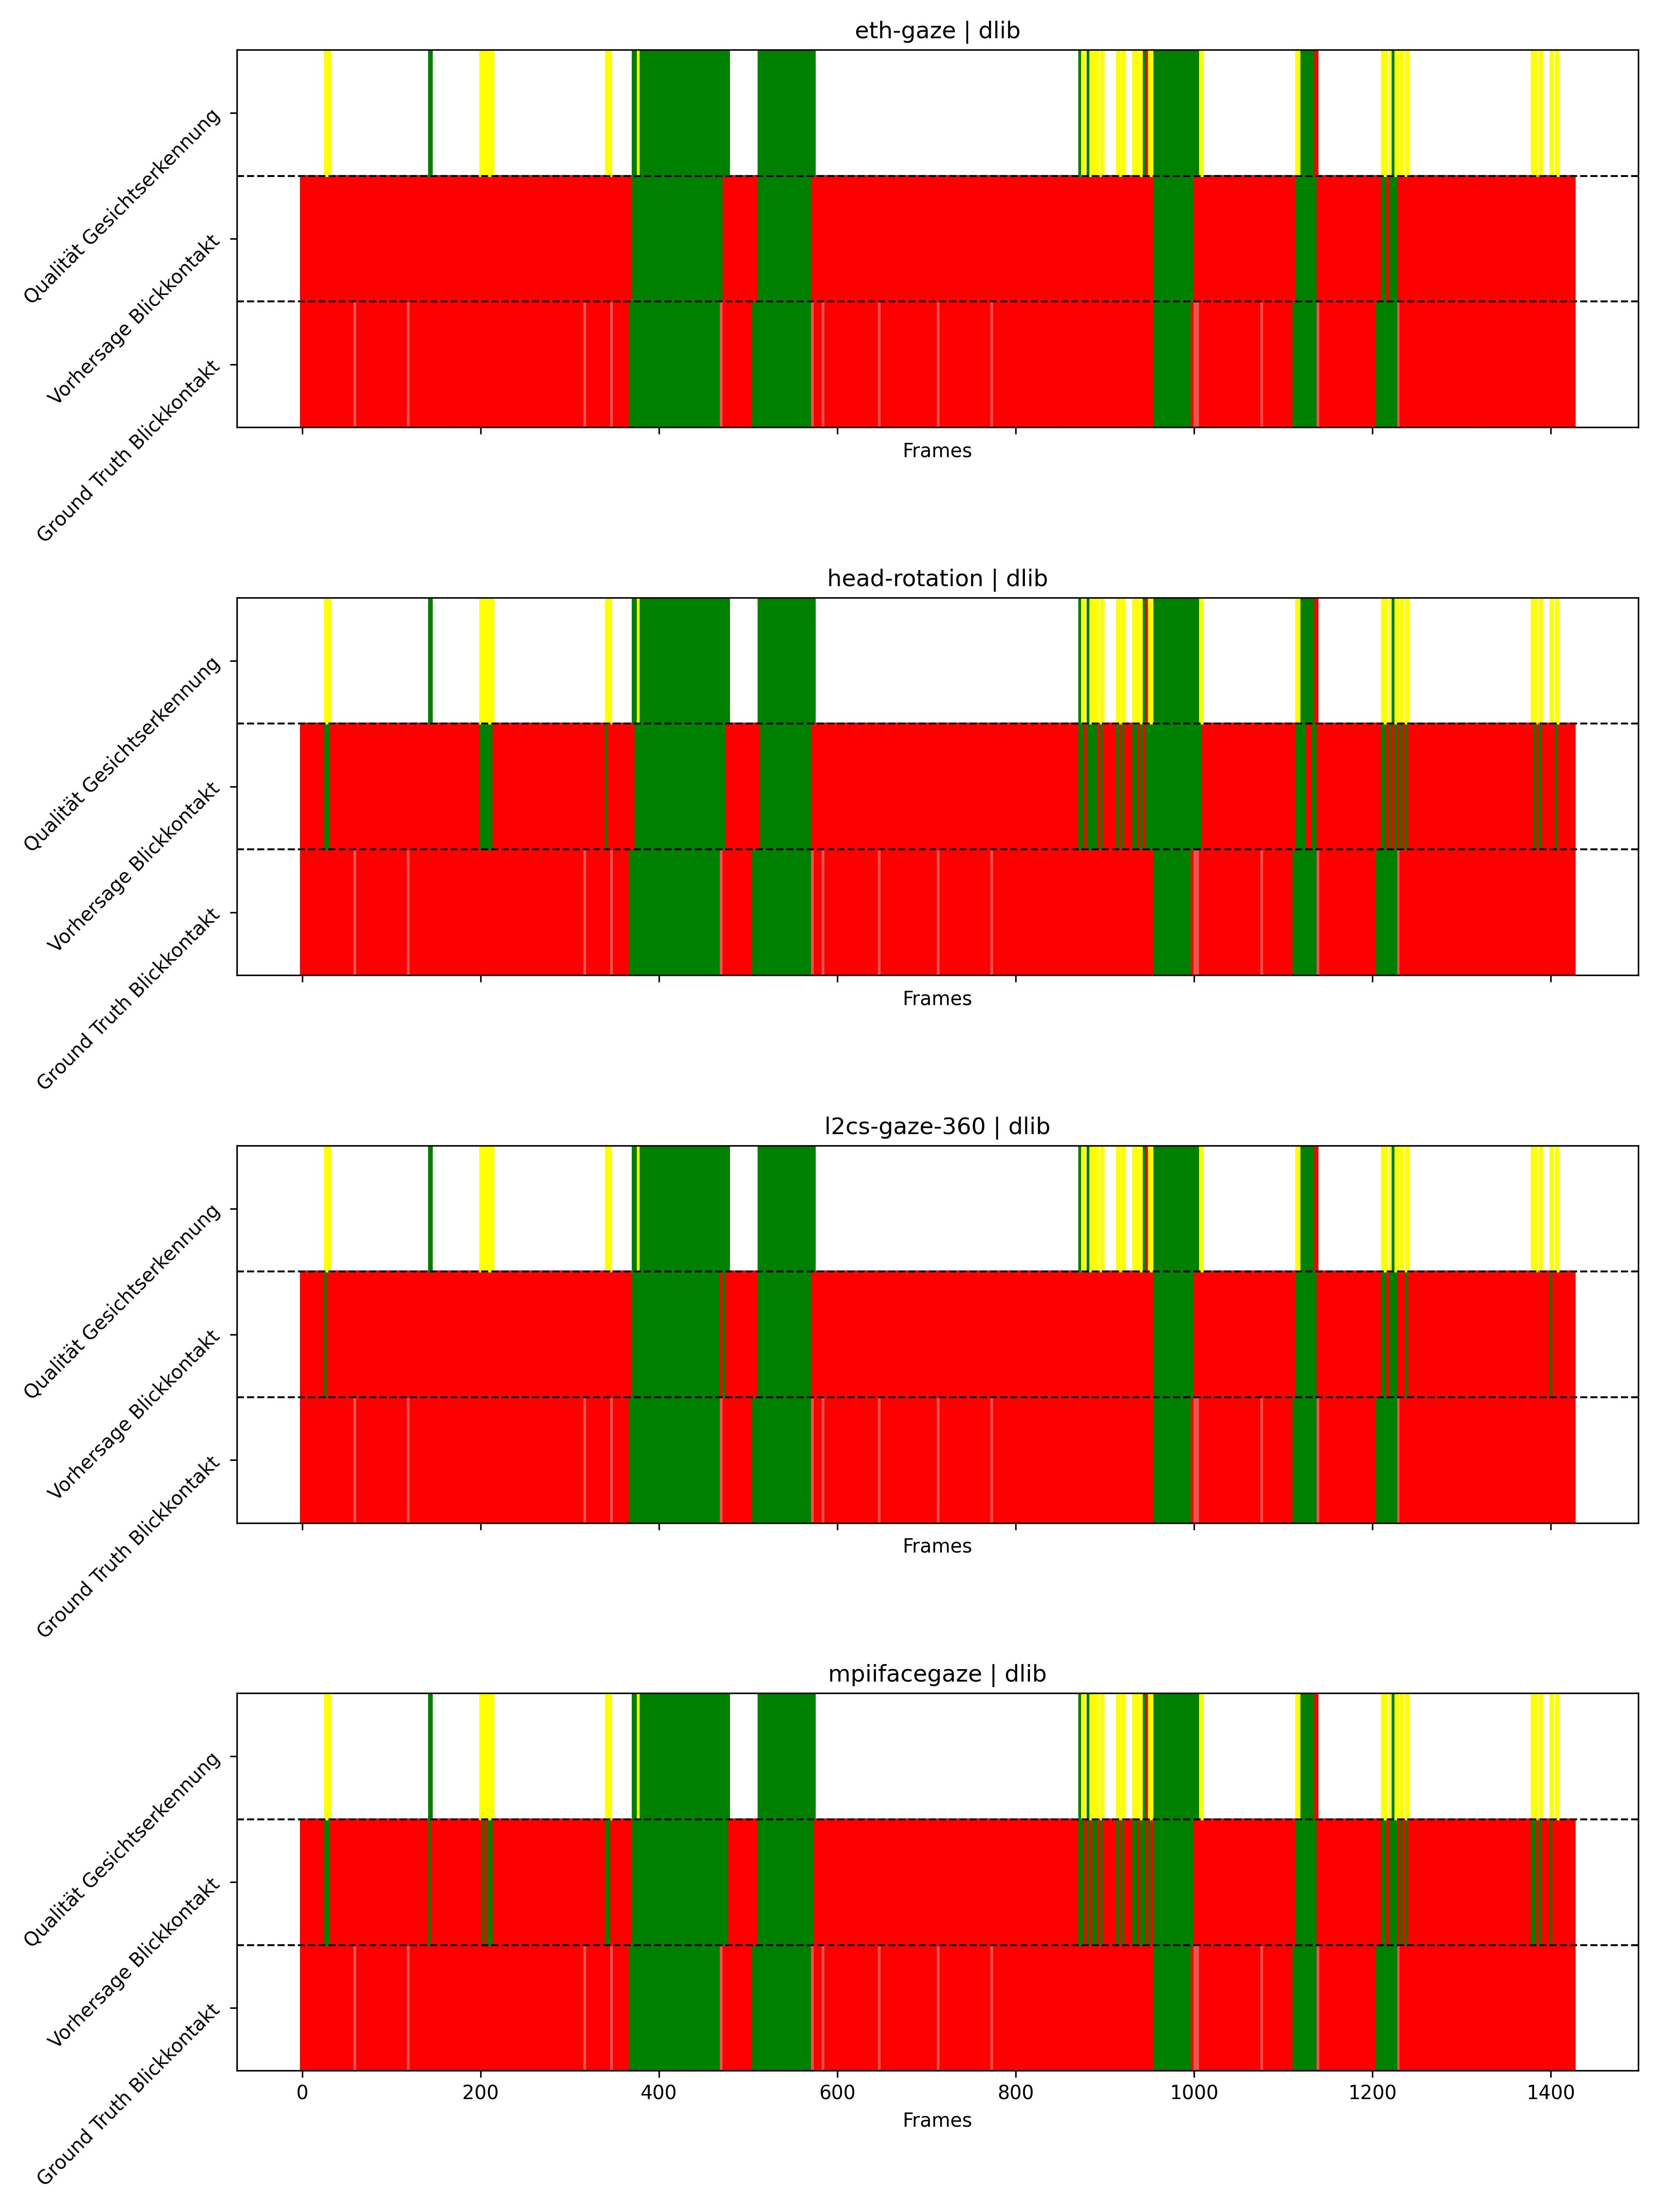
\includegraphics[width=1\linewidth]{appendix/01-dlib-overview-gaze.jpg}
\caption{Überblick über die Ground Truth des Blickkontakts, die Vorhersage des Blickkontakts und die Qualität der Gesichtserkennung mit \dlib. Die Bedeutung der Farben ist in Abbildung \ref{fig:evaluation:gaze:mpiifacegaze} erklärt.  }
\end{figure}

\begin{figure}[H]
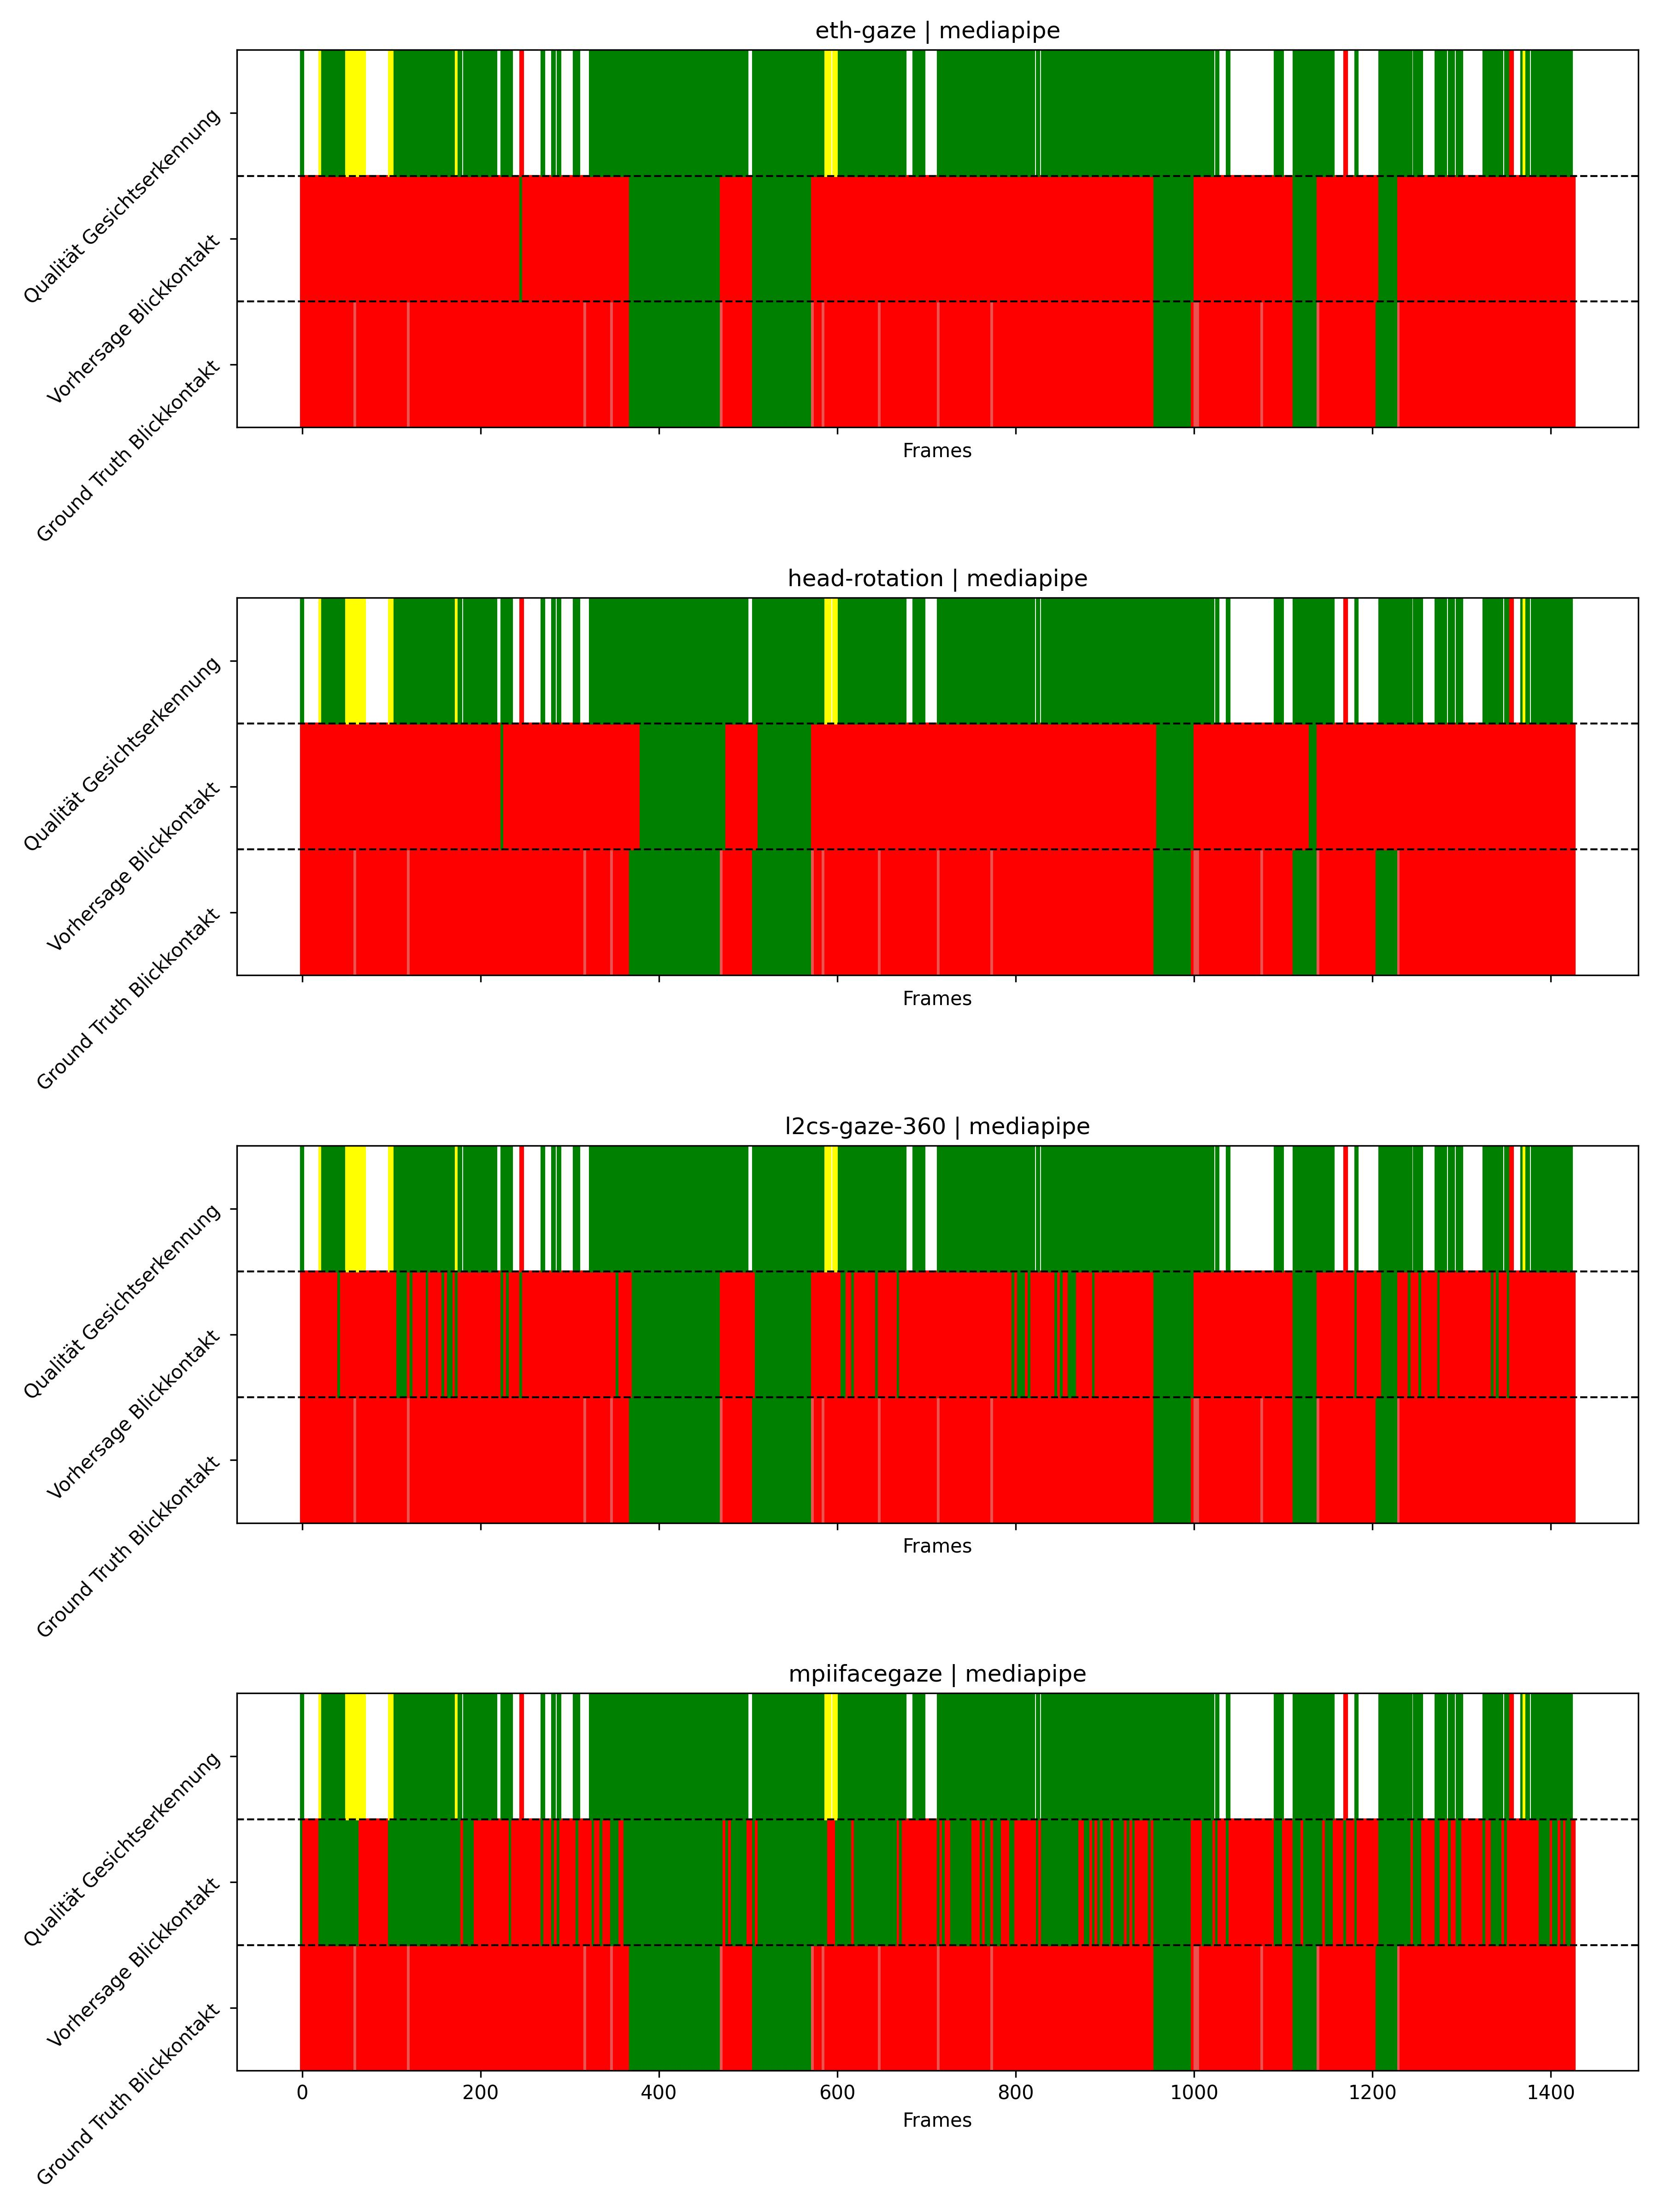
\includegraphics[width=1\linewidth]{appendix/01-mediapipe-overview-gaze.jpg}
\caption{Überblick über die Ground Truth des Blickkontakts, die Vorhersage des Blickkontakts und die Qualität der Gesichtserkennung mit \mediapipe. Die Bedeutung der Farben ist in Abbildung \ref{fig:evaluation:gaze:mpiifacegaze} erklärt.}
\end{figure}

\section{Video 02}
\begin{figure}[H]
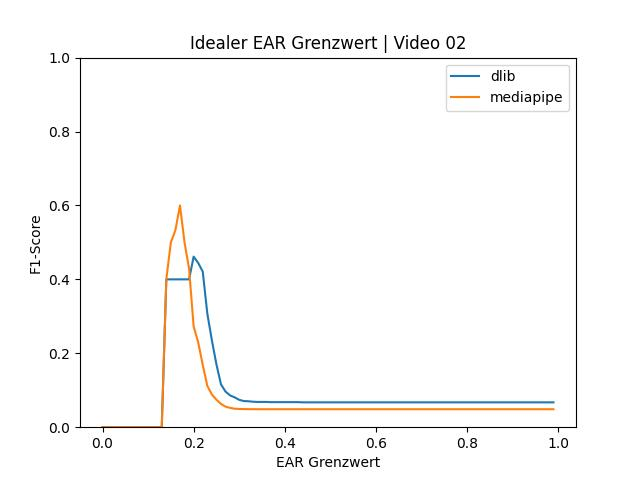
\includegraphics[width=0.7\linewidth]{appendix/02_f1-score-blink.jpg}
\caption{Ergebnisse der Bestimmung des idealen EAR-Grenzwerts für Video 02.}
\end{figure}

\begin{figure}[H]
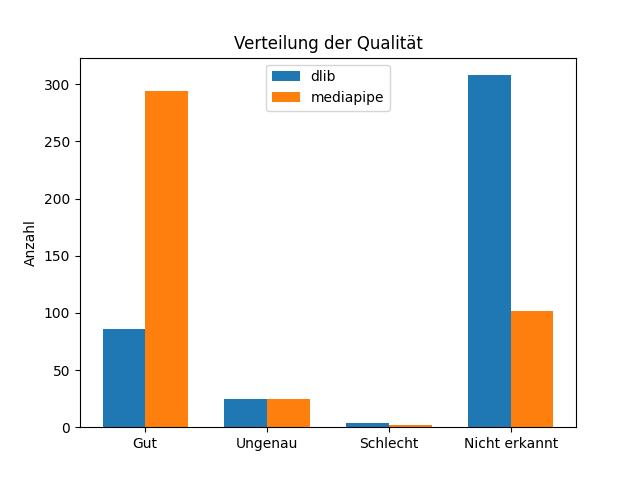
\includegraphics[width=0.7\linewidth]{appendix/02_bar-quality.jpg}
\caption{Aufteilung der Gesichtserkennungsqualität von Video 02.}
\end{figure}

\begin{table}[H]
\centering
\begin{tabular}{l|l|c c |c}
\toprule
\textbf{Gesichtserkennung} & \textbf{Blickrichtung} & \textbf{Seitenlänge} $\hitthresholdsize$ & \textbf{Verschiebung} $\hitthresholdposition$ & \textbf{F1-Score} \\ 
\midrule
\multirow{4}*{dlib}& ETH-XGaze & 0,092 & -0,014 & 0,956  \\ 
& Gaze360 & 0,286 & 0,047 & 0,906 \\ 
& MPIIFaceGaze & 0,031 & -0,027 & 0,785  \\ 
& Kopfrotation & 0,071 & 0,182 & 0,807  \\ 
\hline\multirow{4}*{MediaPipe}& ETH-XGaze & 0,092 & -0,014 & 0,974  \\ 
& Gaze360 & 0,255 & 0,047 & 0,862 \\ 
& MPIIFaceGaze & 0,031 & -0,027 & 0,591  \\ 
& Kopfrotation & 0,143 & 0,206 & 0,911  \\ 
\bottomrule\end{tabular}
\caption{Ergebnis des Hyperparameter-Tunings für die Zone speziell für Video 02.}
\label{tab:appendix:02:local}
\end{table}
\begin{table}[H]
\centering
\begin{tabular}{l|l|c c c c|c c|c}
\toprule
\textbf{Gesichtserkennung} & \textbf{Blickrichtung} & $TP$ & $TN$& $FP$ & $FN$ & \textbf{Precision} & \textbf{Recall} & \textbf{F1-Score} \\ 
\midrule
\multirow{4}*{dlib}& ETH-XGaze & 54 & 360 & 3 & 3 & 0,947 & 0,947 & 0,947 \\ 
& Gaze360 & 53 & 351 & 12 & 4 & 0,815 & 0,93 & 0,869 \\ 
& MPIIFaceGaze & 54 & 326 & 37 & 3 & 0,593 & 0,947 & 0,73 \\ 
& Kopfrotation & 52 & 329 & 34 & 5 & 0,605 & 0,912 & 0,727 \\ 
\hline\multirow{4}*{MediaPipe}& ETH-XGaze & 58 & 358 & 7 & 0 & 0,892 & 1,0 & 0,943 \\ 
& Gaze360 & 52 & 352 & 13 & 6 & 0,8 & 0,897 & 0,846 \\ 
& MPIIFaceGaze & 56 & 218 & 147 & 2 & 0,276 & 0,966 & 0,429 \\ 
& Kopfrotation & 51 & 361 & 4 & 7 & 0,927 & 0,879 & 0,903 \\ 
\bottomrule\end{tabular}
\caption{Zusammensetzung des F1-Scores unter Verwendung der in Kapitel \ref{sec:evaluation:results:gaze:threshold} bestimmten globalen Parameter $\hitthresholdsize$ und $\hitthresholdposition$.}
\label{tab:appendix:02:f1}
\end{table}
\begin{figure}[H]
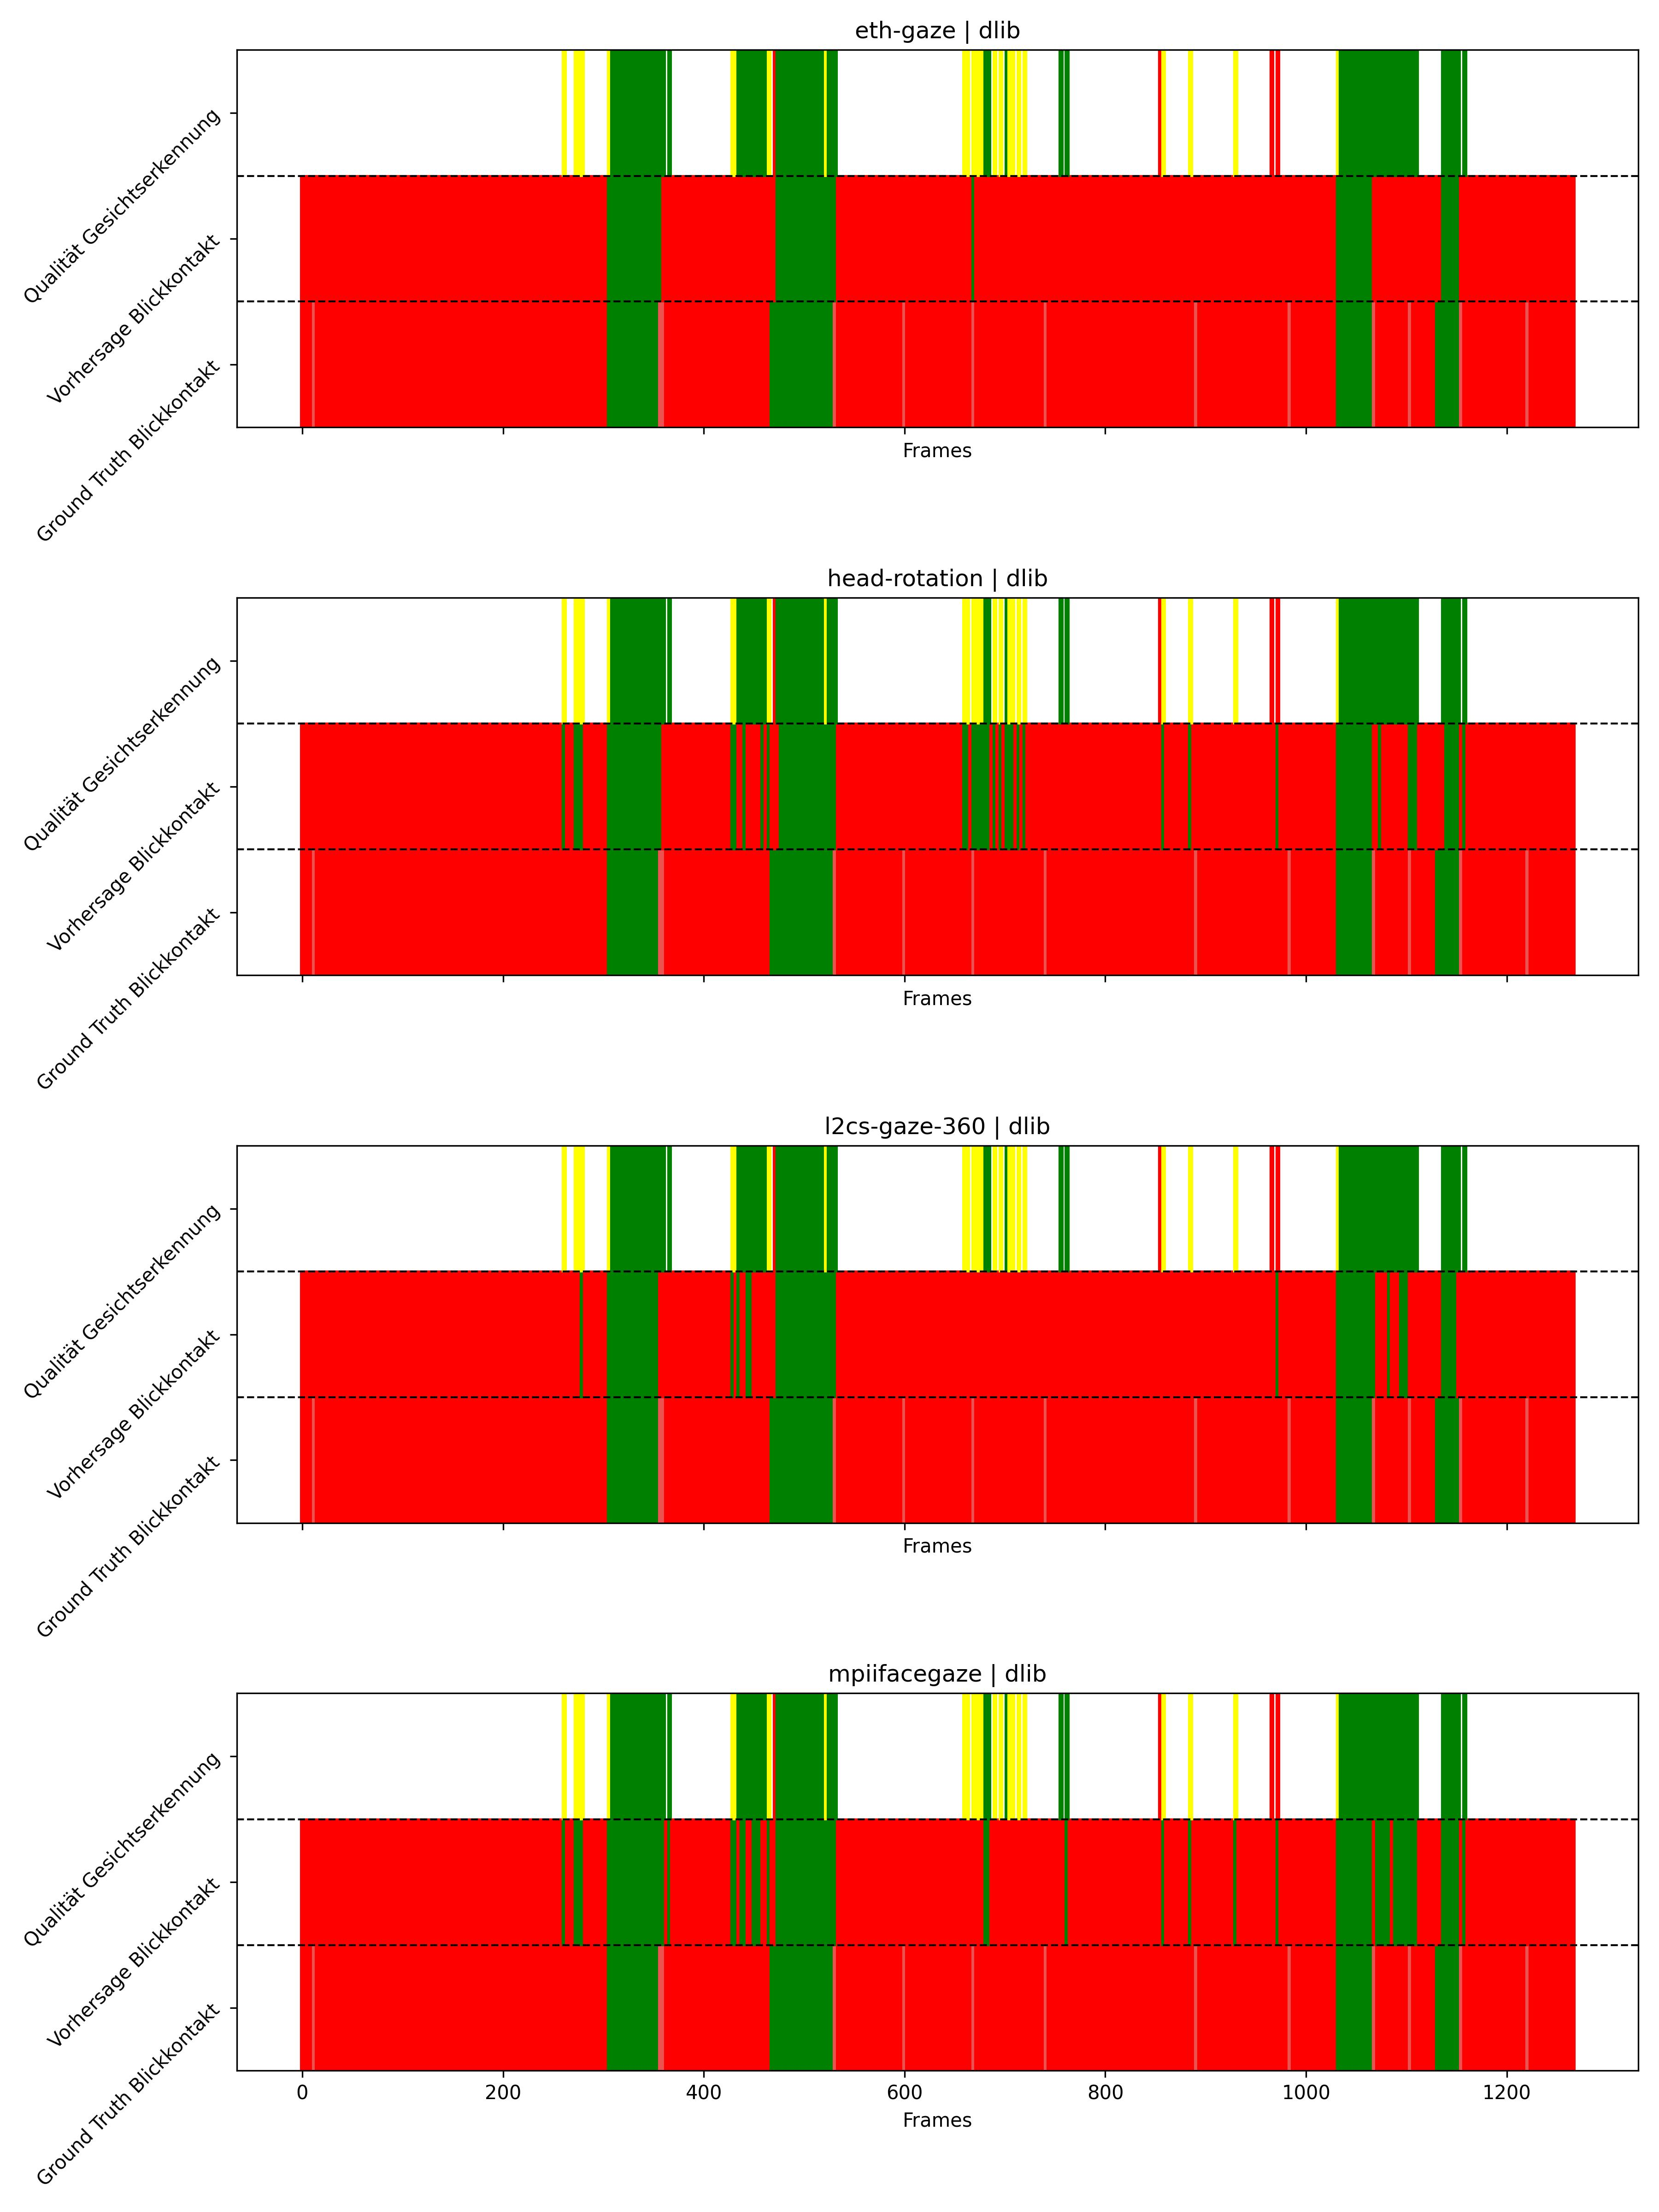
\includegraphics[width=1\linewidth]{appendix/02-dlib-overview-gaze.jpg}
\caption{Überblick über die Ground Truth des Blickkontakts, die Vorhersage des Blickkontakts und die Qualität der Gesichtserkennung mit \dlib. Die Bedeutung der Farben ist in Abbildung \ref{fig:evaluation:gaze:mpiifacegaze} erklärt.  }
\end{figure}

\begin{figure}[H]
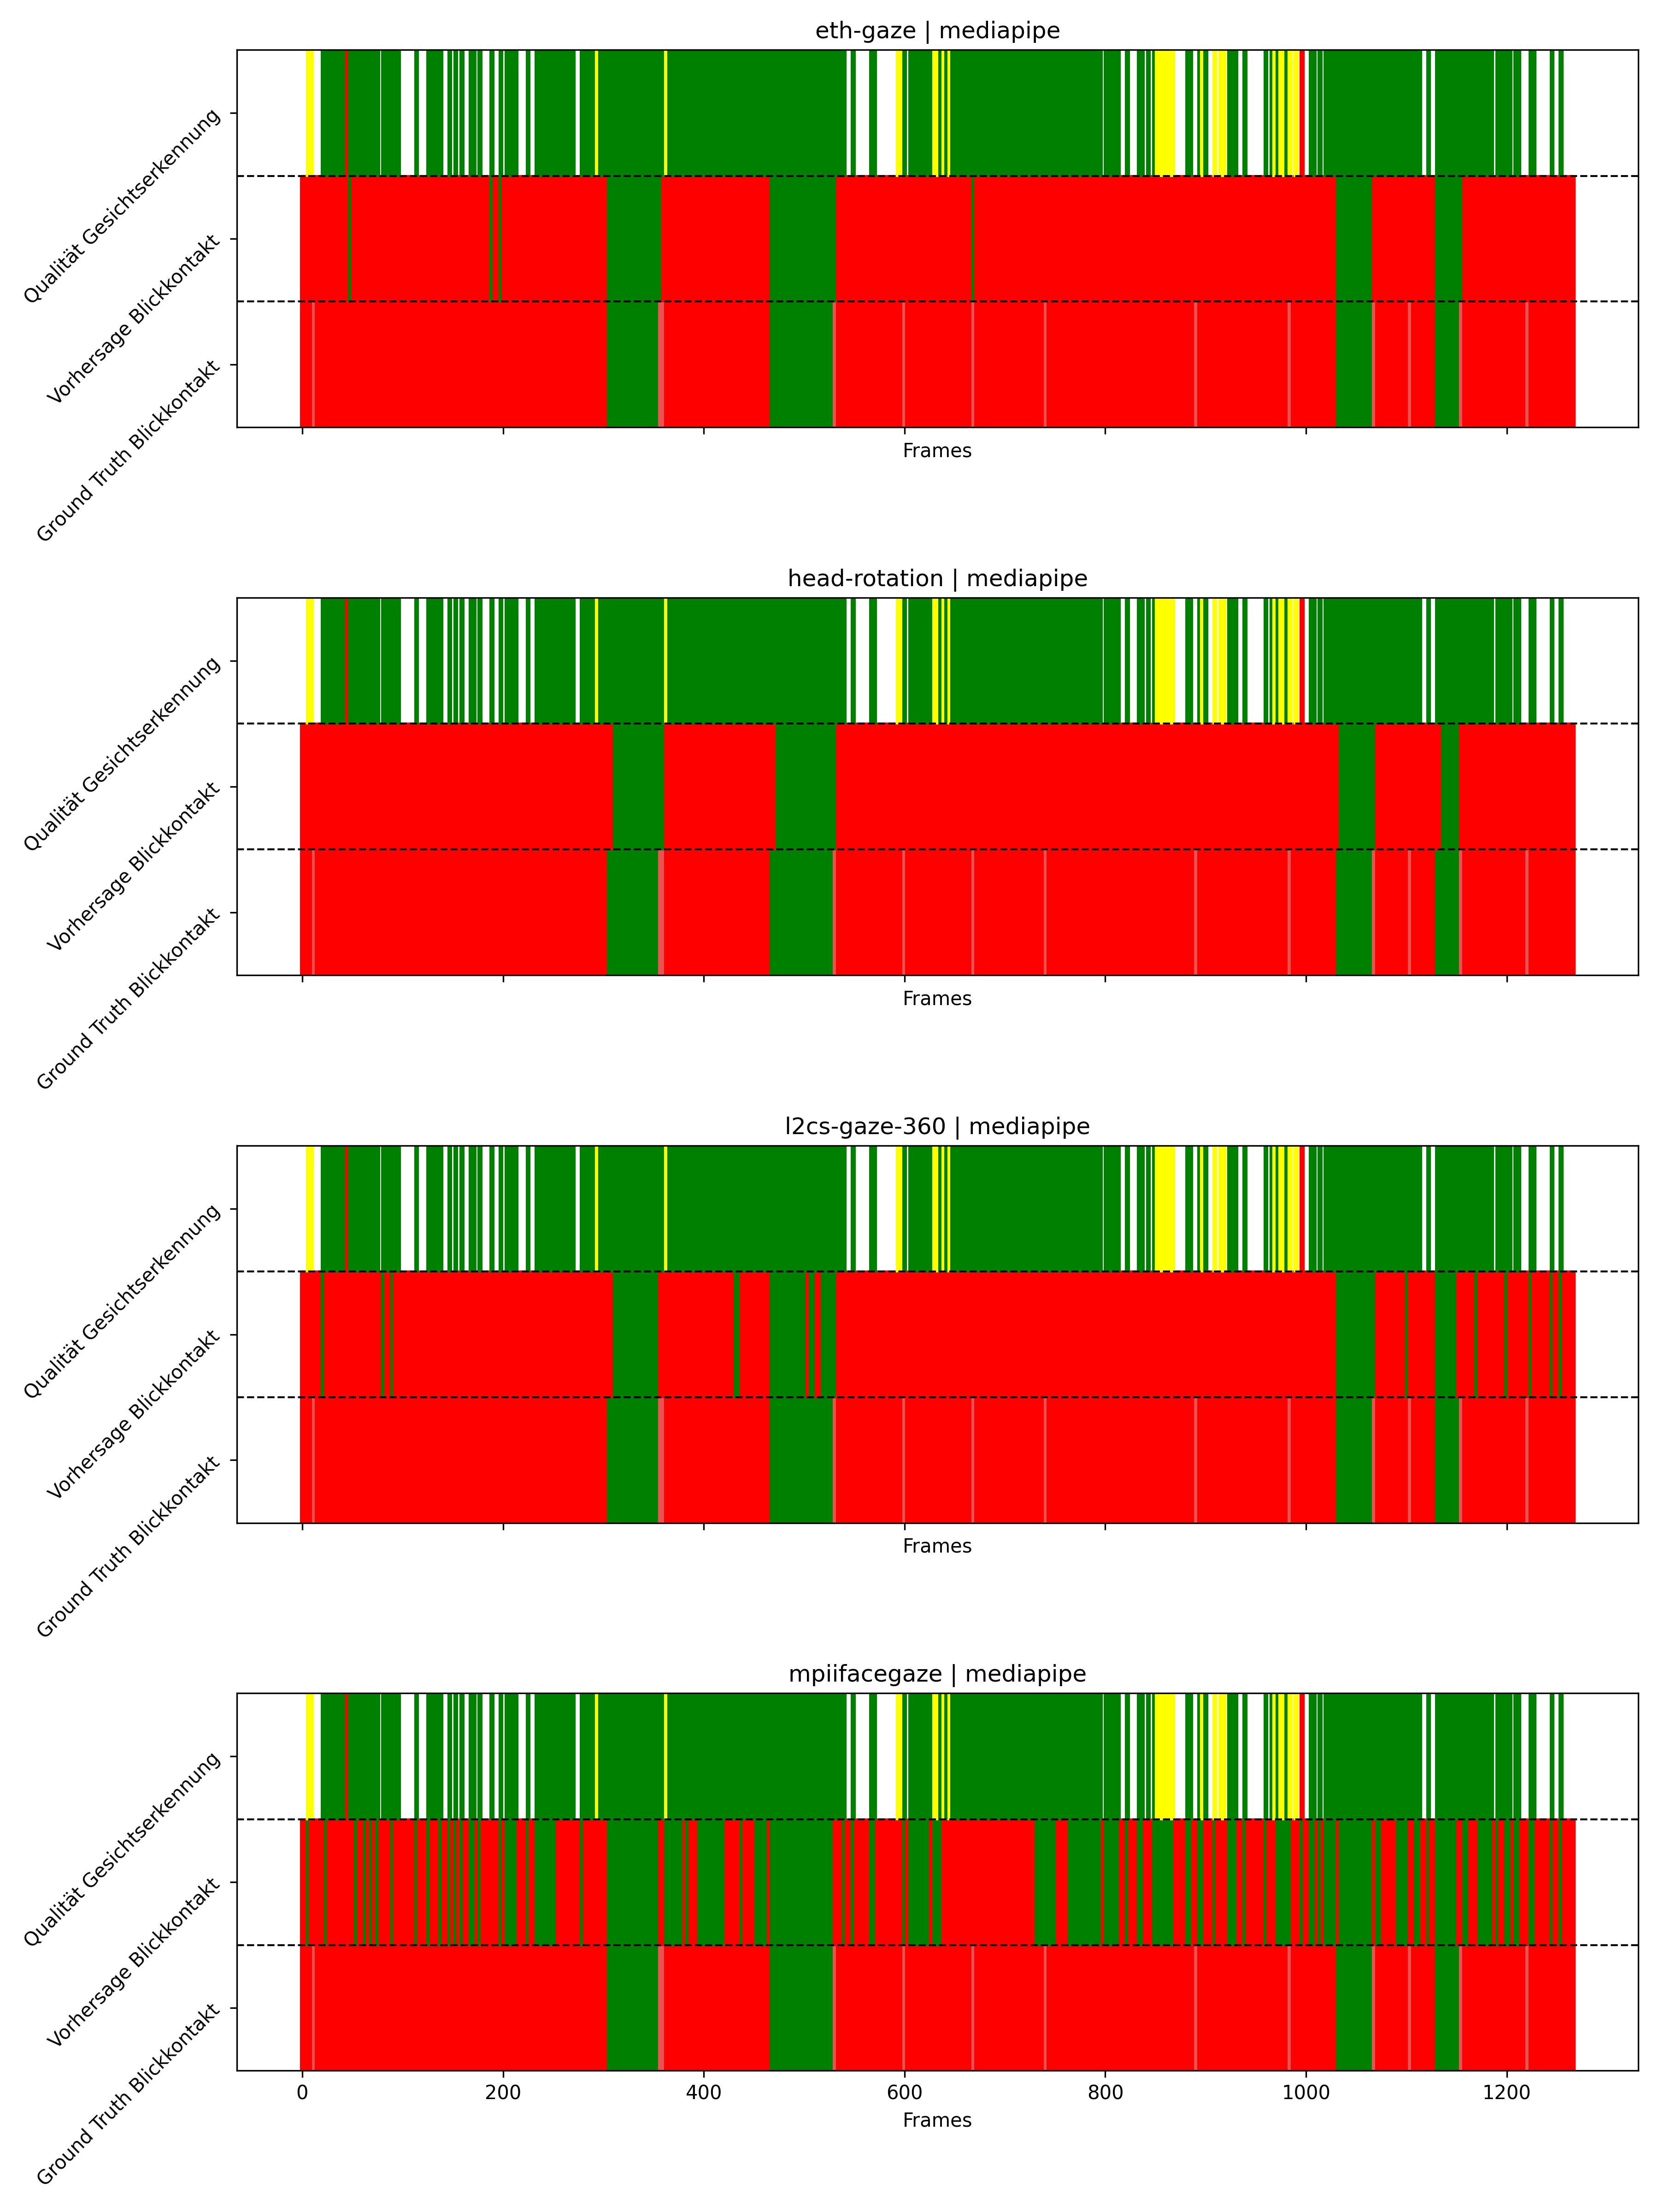
\includegraphics[width=1\linewidth]{appendix/02-mediapipe-overview-gaze.jpg}
\caption{Überblick über die Ground Truth des Blickkontakts, die Vorhersage des Blickkontakts und die Qualität der Gesichtserkennung mit \mediapipe. Die Bedeutung der Farben ist in Abbildung \ref{fig:evaluation:gaze:mpiifacegaze} erklärt.}
\end{figure}

\section{Video 03}
\begin{figure}[H]
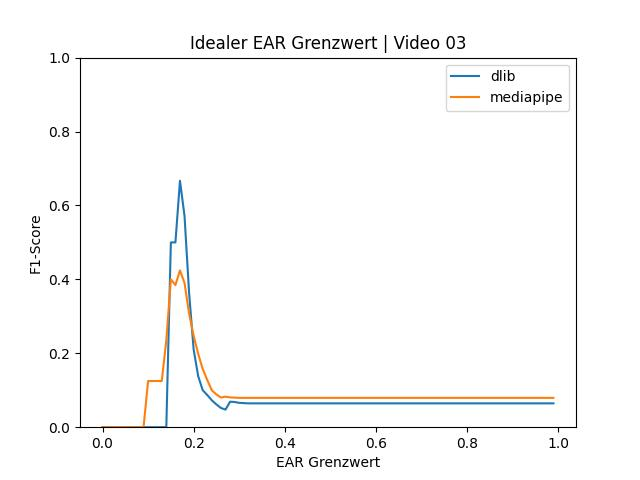
\includegraphics[width=0.7\linewidth]{appendix/03_f1-score-blink.jpg}
\caption{Ergebnisse der Bestimmung des idealen EAR-Grenzwerts für Video 03.}
\end{figure}

\begin{figure}[H]
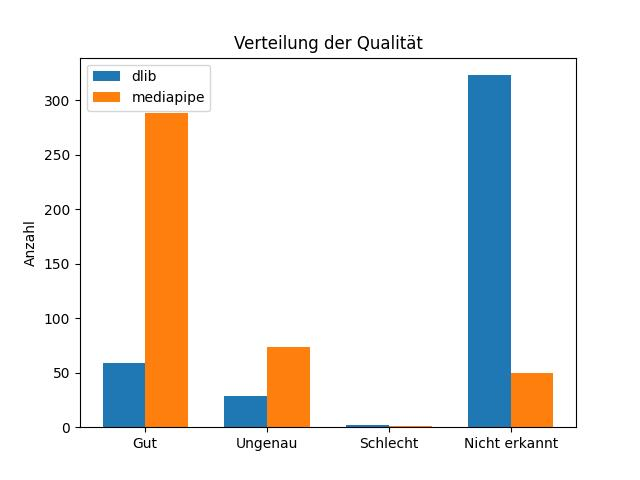
\includegraphics[width=0.7\linewidth]{appendix/03_bar-quality.jpg}
\caption{Aufteilung der Gesichtserkennungsqualität von Video 03.}
\end{figure}

\begin{table}[H]
\centering
\begin{tabular}{l|l|c c |c}
\toprule
\textbf{Gesichtserkennung} & \textbf{Blickrichtung} & \textbf{Seitenlänge} $\hitthresholdsize$ & \textbf{Verschiebung} $\hitthresholdposition$ & \textbf{F1-Score} \\ 
\midrule
\multirow{4}*{dlib}& ETH-XGaze & 0,061 & -0,039 & 0,972  \\ 
& Gaze360 & 0,214 & 0,035 & 0,907 \\ 
& MPIIFaceGaze & 0,02 & -0,039 & 0,683  \\ 
& Kopfrotation & 0,102 & 0,194 & 0,895  \\ 
\hline\multirow{4}*{MediaPipe}& ETH-XGaze & 0,092 & -0,014 & 0,986  \\ 
& Gaze360 & 0,214 & 0,035 & 0,695 \\ 
& MPIIFaceGaze & 0,02 & -0,039 & 0,525  \\ 
& Kopfrotation & 0,112 & 0,206 & 0,971  \\ 
\bottomrule\end{tabular}
\caption{Ergebnis des Hyperparameter-Tunings für die Zone speziell für Video 03.}
\label{tab:appendix:03:local}
\end{table}
\begin{table}[H]
\centering
\begin{tabular}{l|l|c c c c|c c|c}
\toprule
\textbf{Gesichtserkennung} & \textbf{Blickrichtung} & $TP$ & $TN$& $FP$ & $FN$ & \textbf{Precision} & \textbf{Recall} & \textbf{F1-Score} \\ 
\midrule
\multirow{4}*{dlib}& ETH-XGaze & 35 & 375 & 2 & 1 & 0,946 & 0,972 & 0,959 \\ 
& Gaze360 & 35 & 365 & 12 & 1 & 0,745 & 0,972 & 0,843 \\ 
& MPIIFaceGaze & 35 & 328 & 49 & 1 & 0,417 & 0,972 & 0,583 \\ 
& Kopfrotation & 34 & 352 & 25 & 2 & 0,576 & 0,944 & 0,716 \\ 
\hline\multirow{4}*{MediaPipe}& ETH-XGaze & 36 & 375 & 2 & 0 & 0,947 & 1,0 & 0,973 \\ 
& Gaze360 & 36 & 319 & 58 & 0 & 0,383 & 1,0 & 0,554 \\ 
& MPIIFaceGaze & 36 & 132 & 245 & 0 & 0,128 & 1,0 & 0,227 \\ 
& Kopfrotation & 34 & 375 & 2 & 2 & 0,944 & 0,944 & 0,944 \\ 
\bottomrule\end{tabular}
\caption{Zusammensetzung des F1-Scores unter Verwendung der in Kapitel \ref{sec:evaluation:results:gaze:threshold} bestimmten globalen Parameter $\hitthresholdsize$ und $\hitthresholdposition$.}
\label{tab:appendix:03:f1}
\end{table}
\begin{figure}[H]
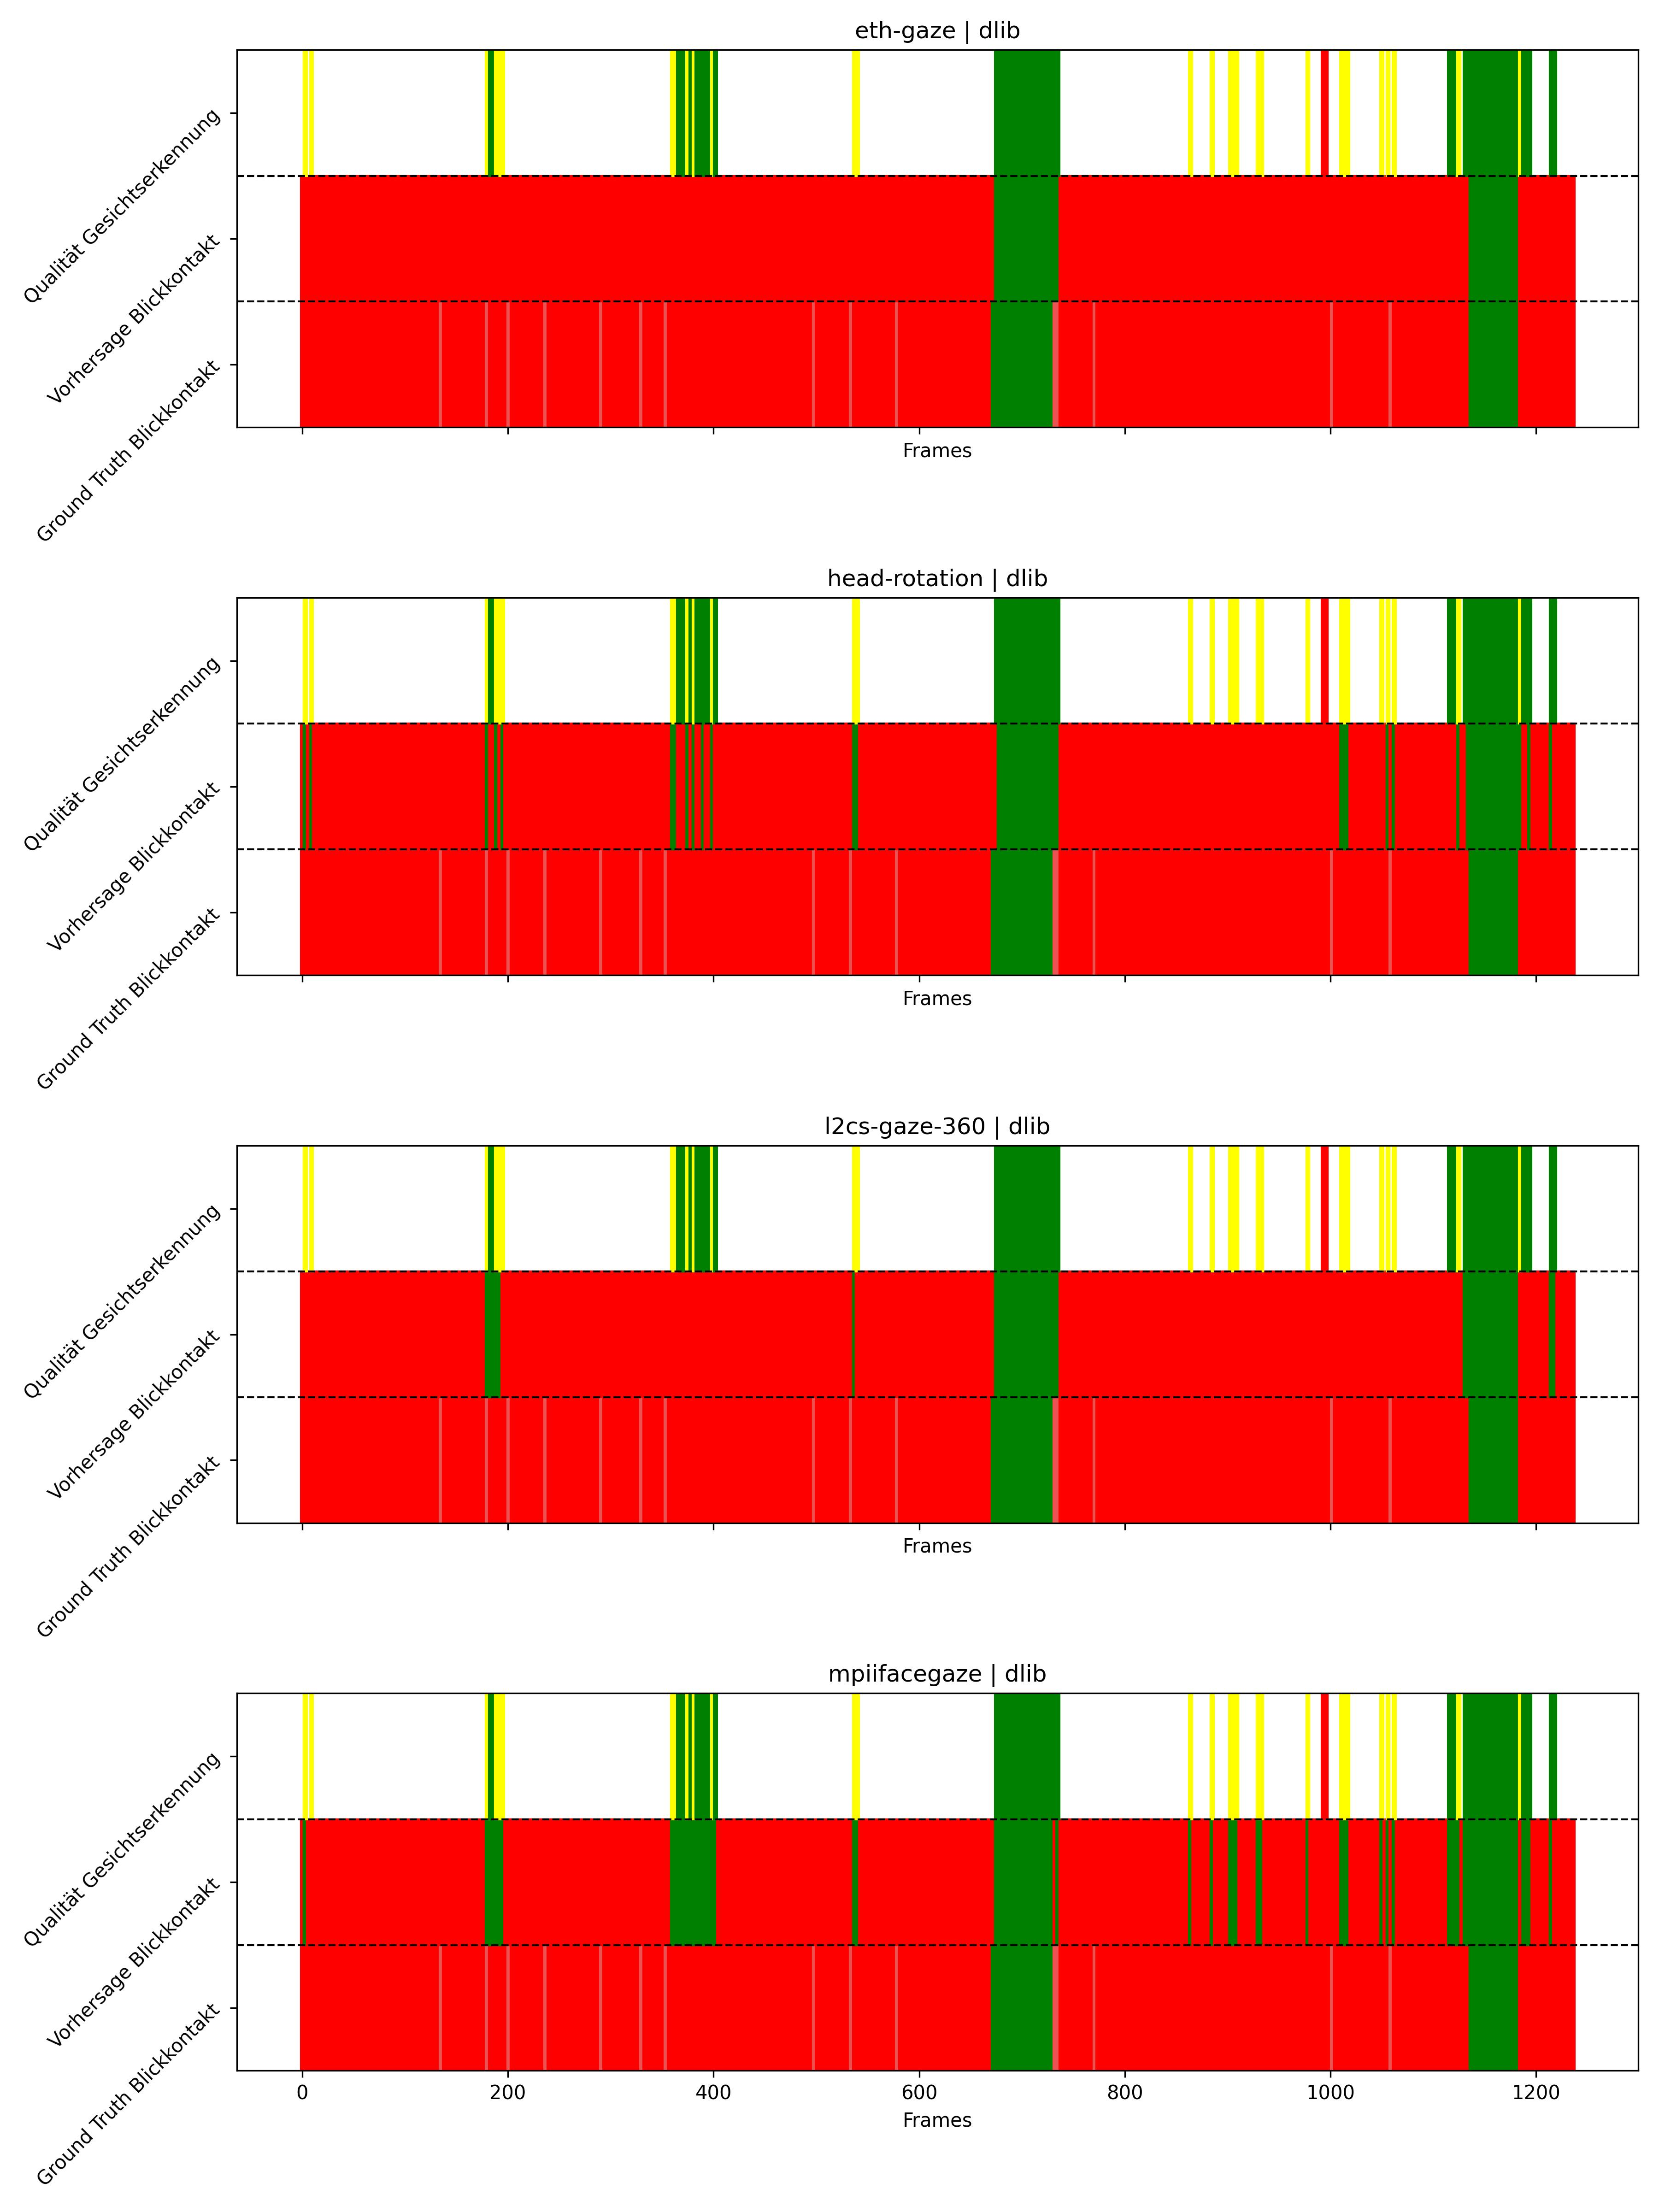
\includegraphics[width=1\linewidth]{appendix/03-dlib-overview-gaze.jpg}
\caption{Überblick über die Ground Truth des Blickkontakts, die Vorhersage des Blickkontakts und die Qualität der Gesichtserkennung mit \dlib. Die Bedeutung der Farben ist in Abbildung \ref{fig:evaluation:gaze:mpiifacegaze} erklärt.  }
\end{figure}

\begin{figure}[H]
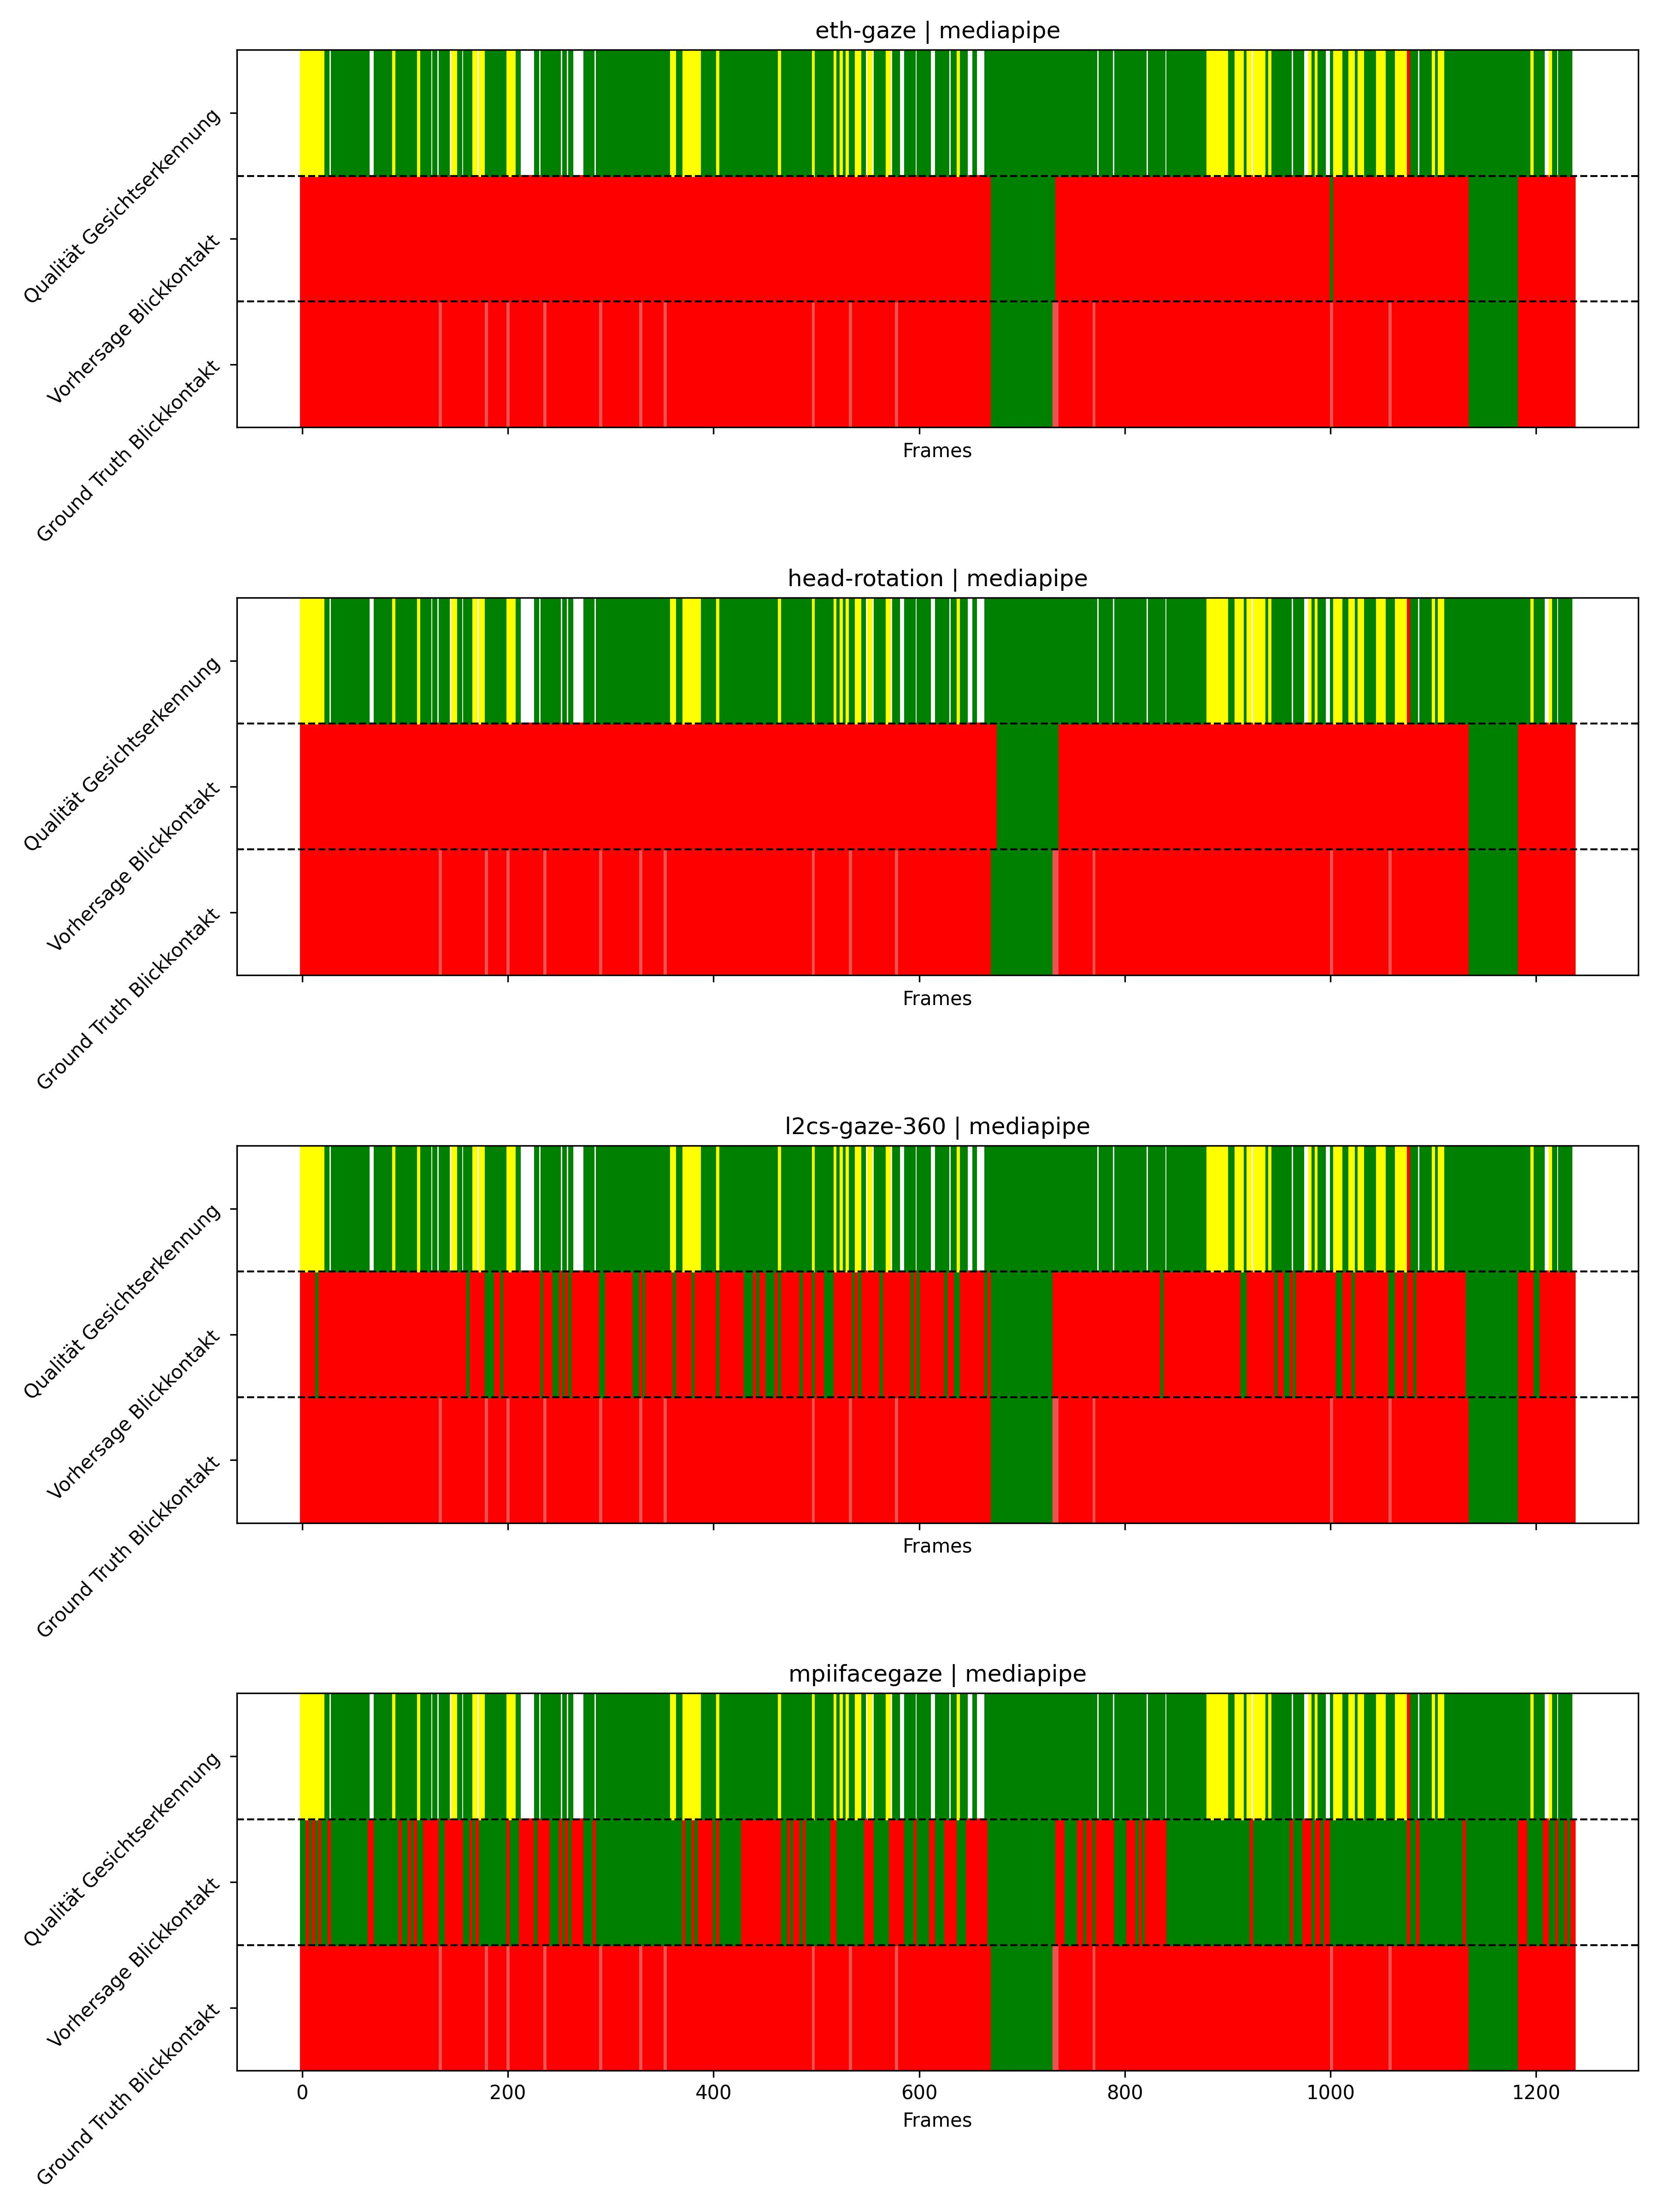
\includegraphics[width=1\linewidth]{appendix/03-mediapipe-overview-gaze.jpg}
\caption{Überblick über die Ground Truth des Blickkontakts, die Vorhersage des Blickkontakts und die Qualität der Gesichtserkennung mit \mediapipe. Die Bedeutung der Farben ist in Abbildung \ref{fig:evaluation:gaze:mpiifacegaze} erklärt.}
\end{figure}

\section{Video 04}
\begin{figure}[H]
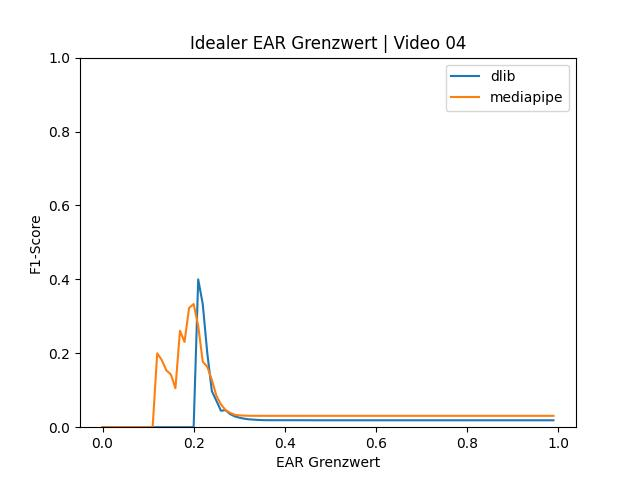
\includegraphics[width=0.7\linewidth]{appendix/04_f1-score-blink.jpg}
\caption{Ergebnisse der Bestimmung des idealen EAR-Grenzwerts für Video 04.}
\end{figure}

\begin{figure}[H]
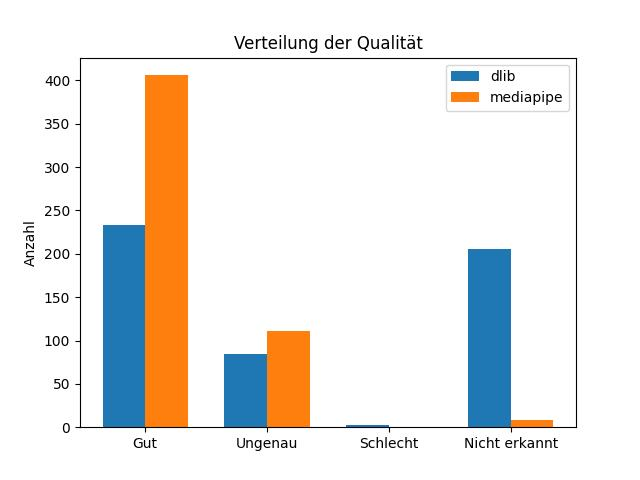
\includegraphics[width=0.7\linewidth]{appendix/04_bar-quality.jpg}
\caption{Aufteilung der Gesichtserkennungsqualität von Video 04.}
\end{figure}

\begin{table}[H]
\centering
\begin{tabular}{l|l|c c |c}
\toprule
\textbf{Gesichtserkennung} & \textbf{Blickrichtung} & \textbf{Seitenlänge} $\hitthresholdsize$ & \textbf{Verschiebung} $\hitthresholdposition$ & \textbf{F1-Score} \\ 
\midrule
\multirow{4}*{dlib}& ETH-XGaze & 0,112 & -0,014 & 0,986  \\ 
& Gaze360 & 0,316 & 0,022 & 0,904 \\ 
& MPIIFaceGaze & 0,041 & -0,027 & 0,536  \\ 
& Kopfrotation & 0,051 & 0,157 & 0,733  \\ 
\hline\multirow{4}*{MediaPipe}& ETH-XGaze & 0,122 & -0,039 & 0,993  \\ 
& Gaze360 & 0,306 & 0,035 & 0,843 \\ 
& MPIIFaceGaze & 0,031 & -0,039 & 0,474  \\ 
& Kopfrotation & 0,082 & 0,157 & 0,853  \\ 
\bottomrule\end{tabular}
\caption{Ergebnis des Hyperparameter-Tunings für die Zone speziell für Video 04.}
\label{tab:appendix:04:local}
\end{table}
\begin{table}[H]
\centering
\begin{tabular}{l|l|c c c c|c c|c}
\toprule
\textbf{Gesichtserkennung} & \textbf{Blickrichtung} & $TP$ & $TN$& $FP$ & $FN$ & \textbf{Precision} & \textbf{Recall} & \textbf{F1-Score} \\ 
\midrule
\multirow{4}*{dlib}& ETH-XGaze & 68 & 449 & 8 & 0 & 0,895 & 1,0 & 0,944 \\ 
& Gaze360 & 67 & 417 & 40 & 1 & 0,626 & 0,985 & 0,766 \\ 
& MPIIFaceGaze & 64 & 342 & 115 & 4 & 0,358 & 0,941 & 0,518 \\ 
& Kopfrotation & 65 & 295 & 162 & 3 & 0,286 & 0,956 & 0,441 \\ 
\hline\multirow{4}*{MediaPipe}& ETH-XGaze & 68 & 448 & 9 & 0 & 0,883 & 1,0 & 0,938 \\ 
& Gaze360 & 67 & 424 & 33 & 1 & 0,67 & 0,985 & 0,798 \\ 
& MPIIFaceGaze & 66 & 265 & 192 & 2 & 0,256 & 0,971 & 0,405 \\ 
& Kopfrotation & 67 & 359 & 98 & 1 & 0,406 & 0,985 & 0,575 \\ 
\bottomrule\end{tabular}
\caption{Zusammensetzung des F1-Scores unter Verwendung der in Kapitel \ref{sec:evaluation:results:gaze:threshold} bestimmten globalen Parameter $\hitthresholdsize$ und $\hitthresholdposition$.}
\label{tab:appendix:04:f1}
\end{table}
\begin{figure}[H]
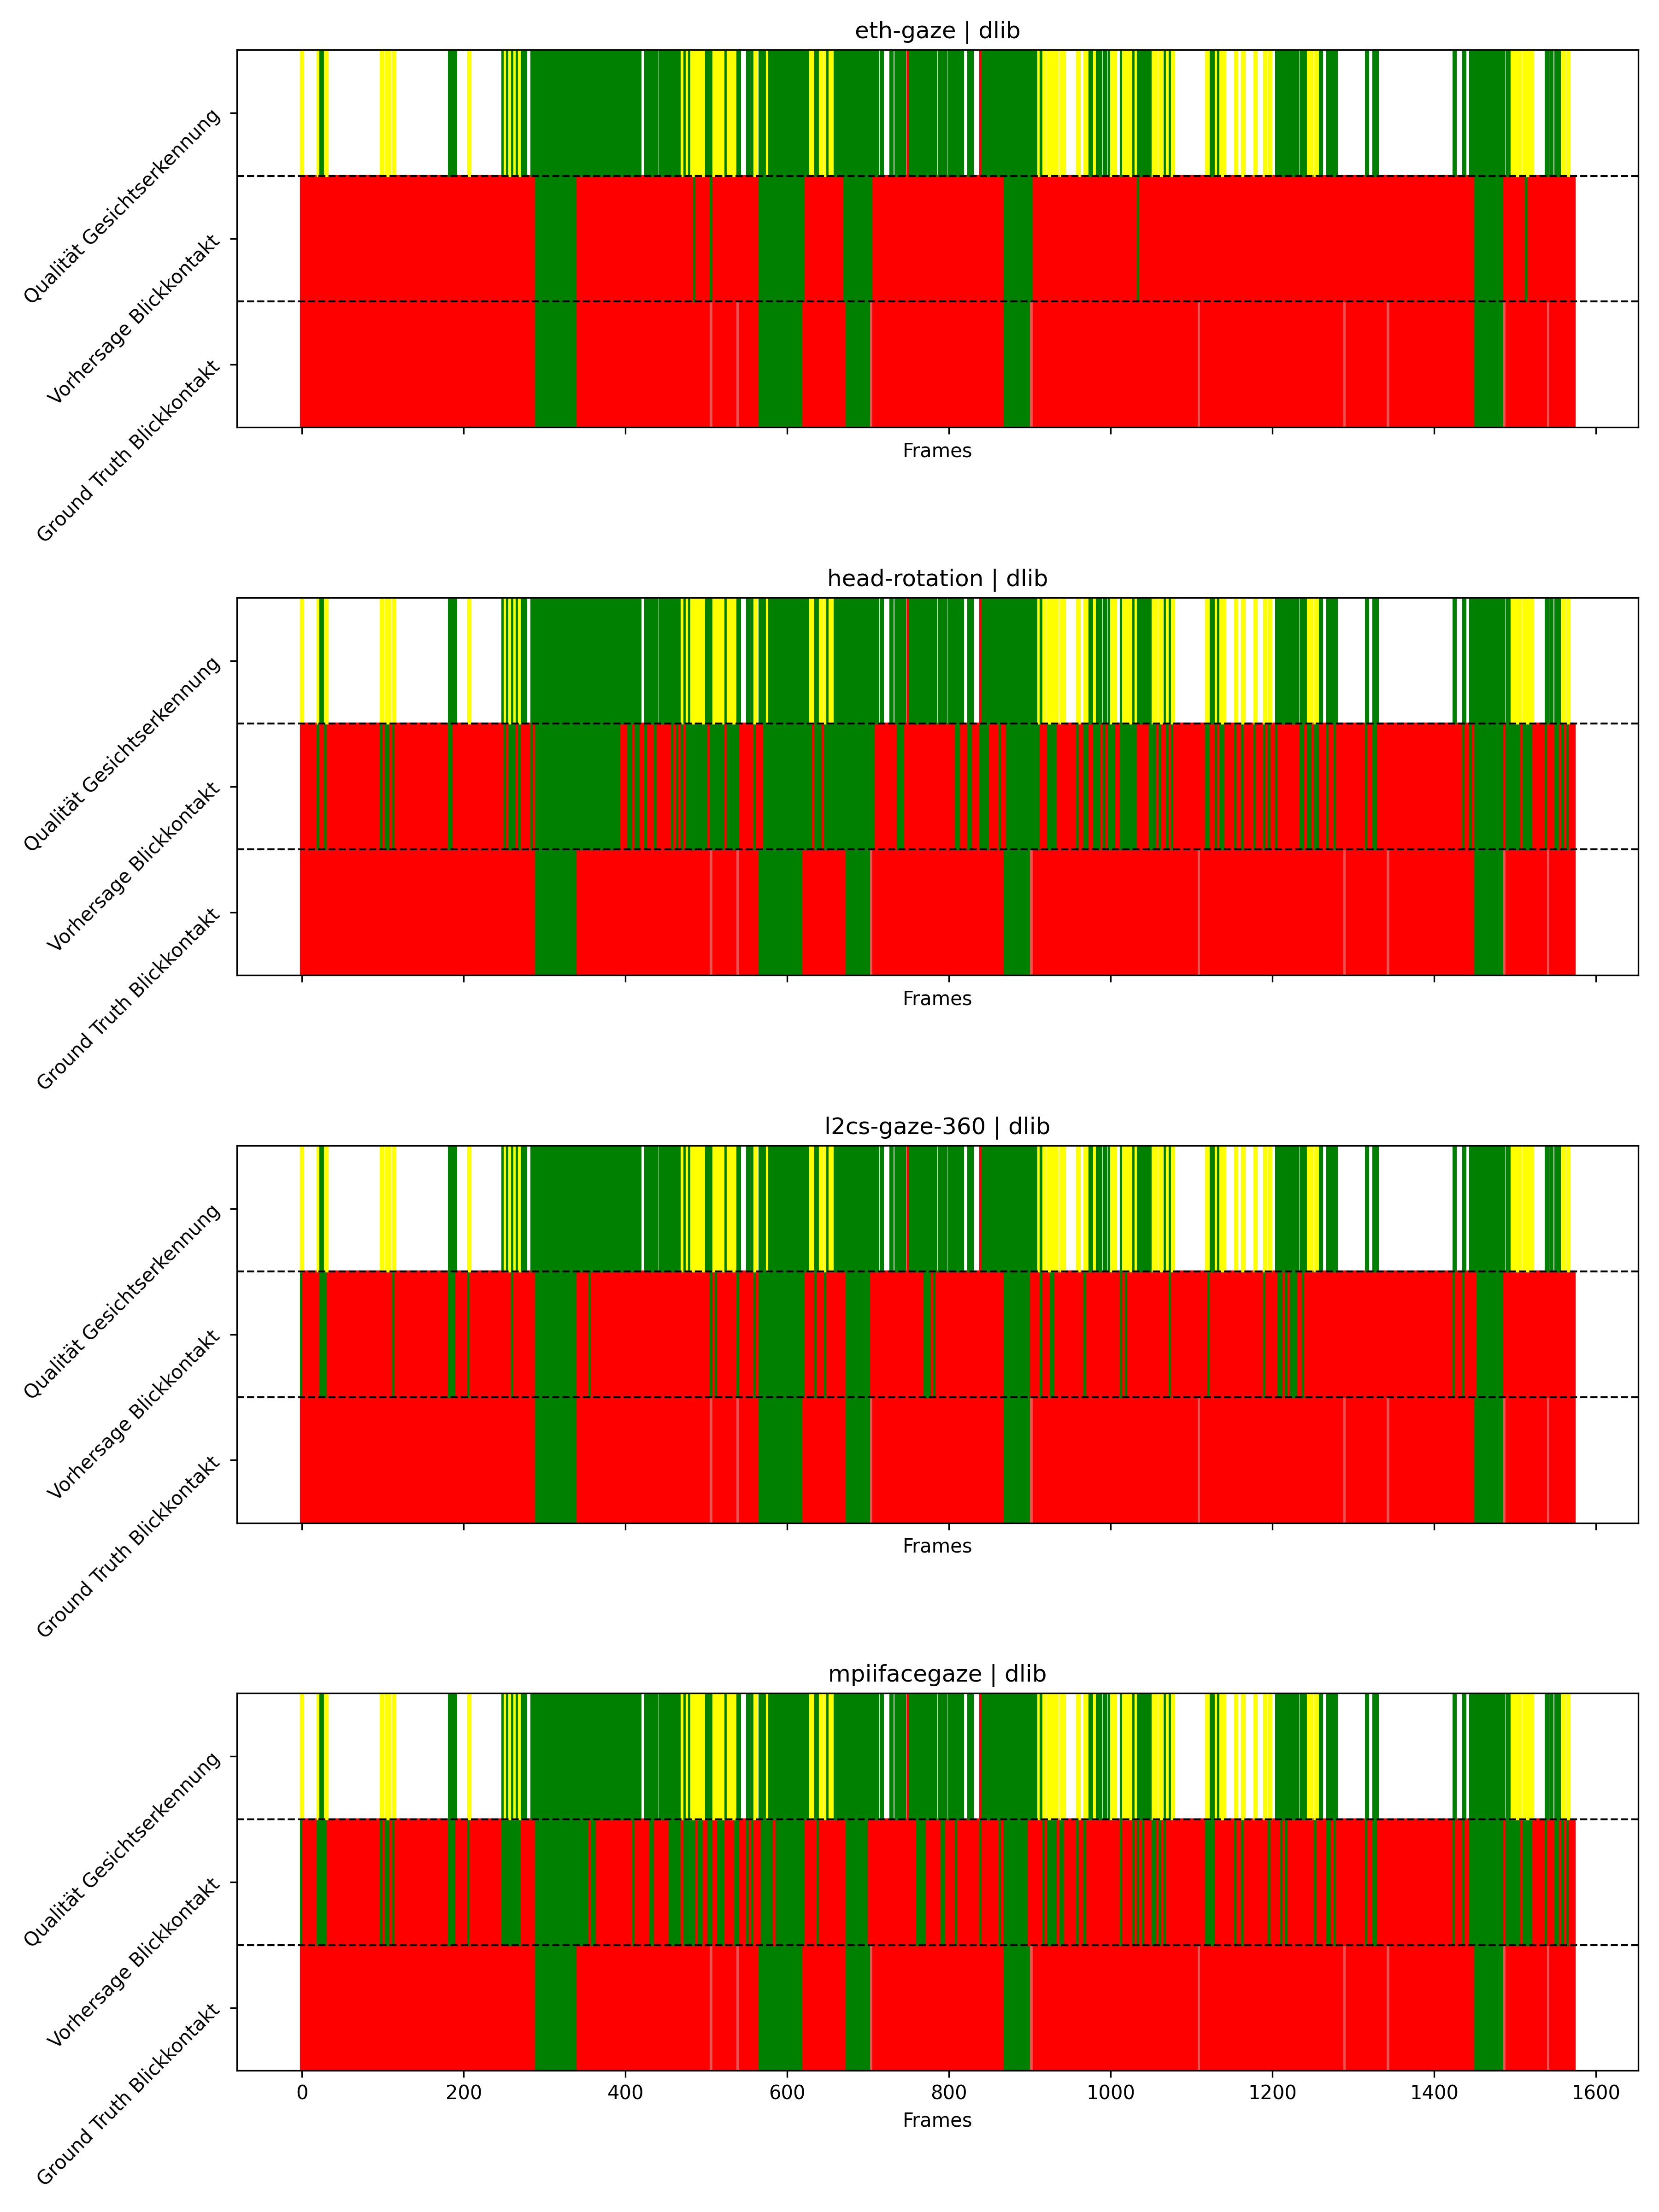
\includegraphics[width=1\linewidth]{appendix/04-dlib-overview-gaze.jpg}
\caption{Überblick über die Ground Truth des Blickkontakts, die Vorhersage des Blickkontakts und die Qualität der Gesichtserkennung mit \dlib. Die Bedeutung der Farben ist in Abbildung \ref{fig:evaluation:gaze:mpiifacegaze} erklärt.  }
\end{figure}

\begin{figure}[H]
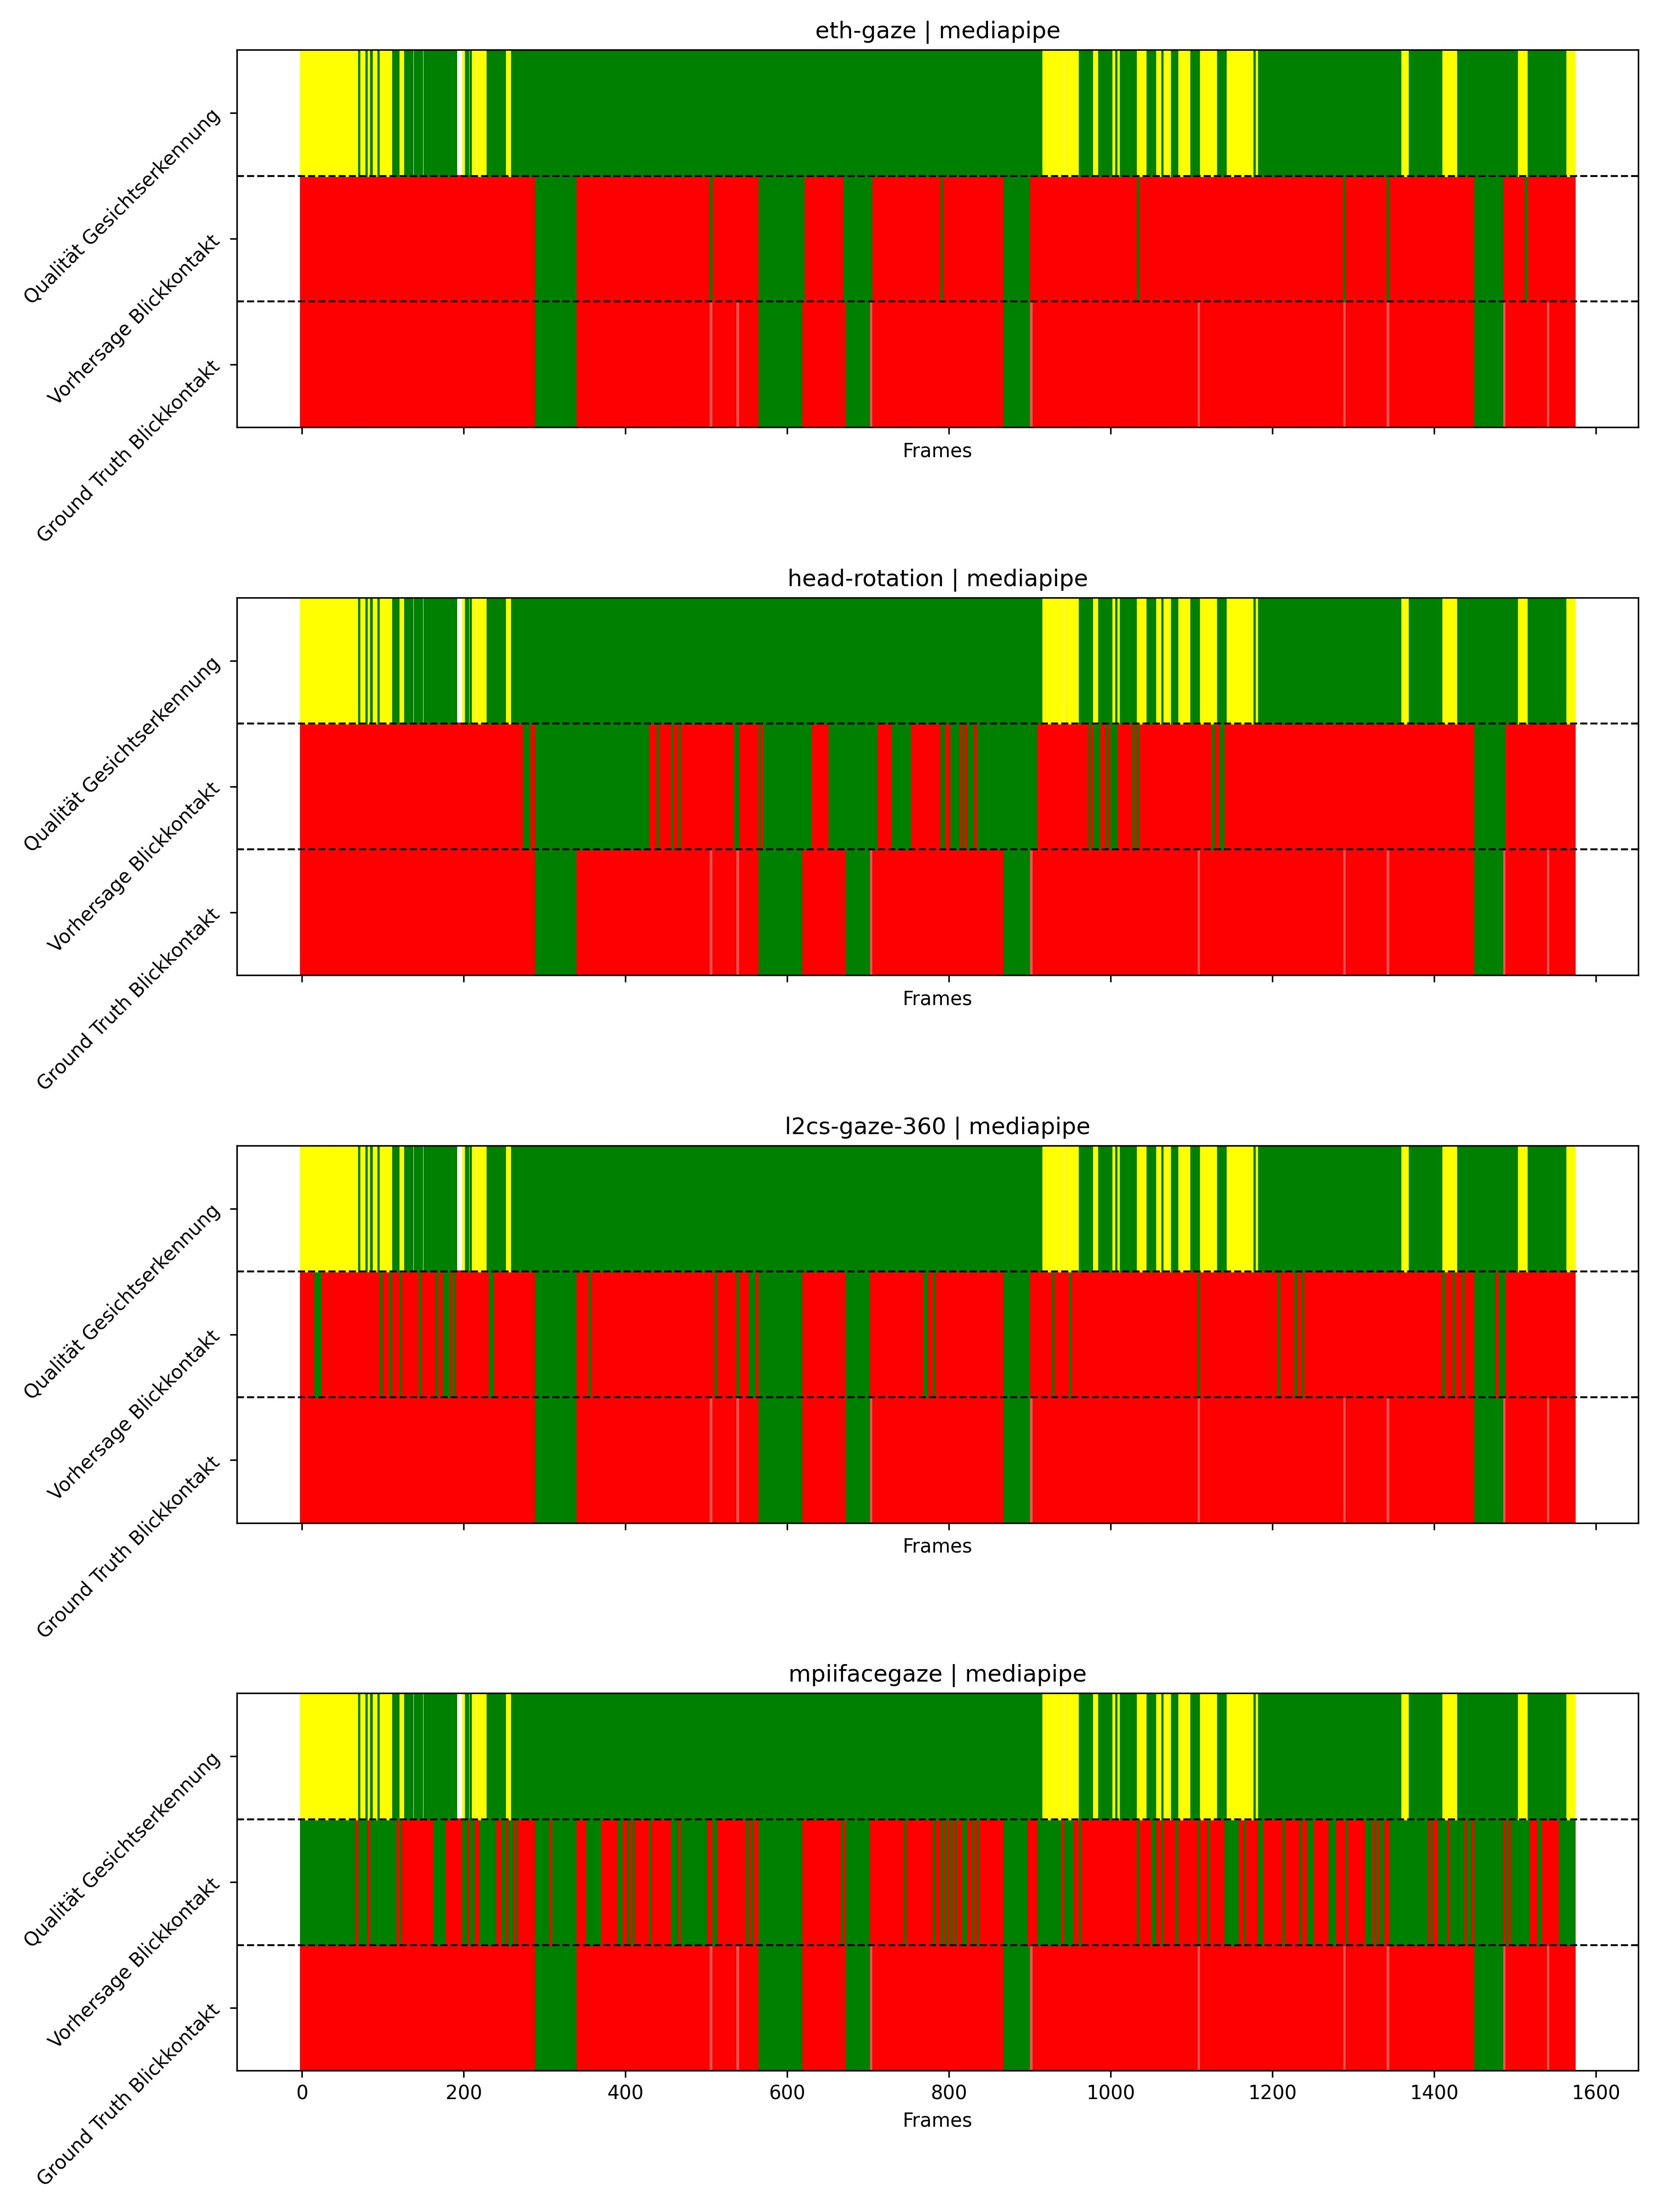
\includegraphics[width=1\linewidth]{appendix/04-mediapipe-overview-gaze.jpg}
\caption{Überblick über die Ground Truth des Blickkontakts, die Vorhersage des Blickkontakts und die Qualität der Gesichtserkennung mit \mediapipe. Die Bedeutung der Farben ist in Abbildung \ref{fig:evaluation:gaze:mpiifacegaze} erklärt.}
\end{figure}

\section{Video 05}
\begin{figure}[H]
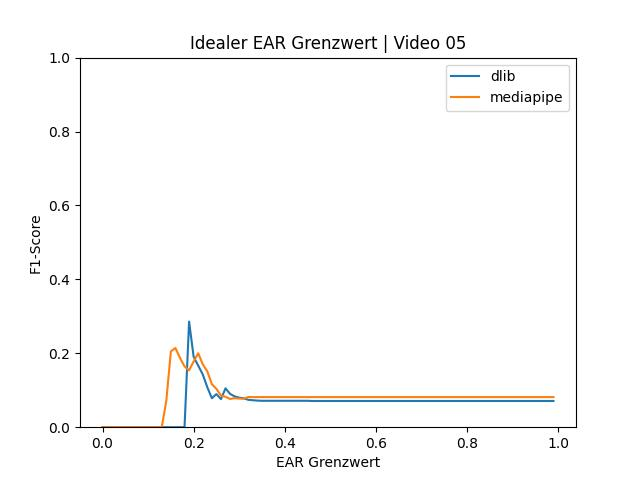
\includegraphics[width=0.7\linewidth]{appendix/05_f1-score-blink.jpg}
\caption{Ergebnisse der Bestimmung des idealen EAR-Grenzwerts für Video 05.}
\end{figure}

\begin{figure}[H]
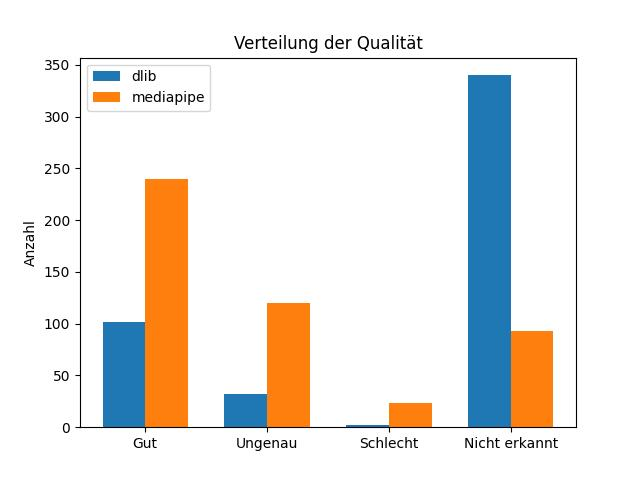
\includegraphics[width=0.7\linewidth]{appendix/05_bar-quality.jpg}
\caption{Aufteilung der Gesichtserkennungsqualität von Video 05.}
\end{figure}

\begin{table}[H]
\centering
\begin{tabular}{l|l|c c |c}
\toprule
\textbf{Gesichtserkennung} & \textbf{Blickrichtung} & \textbf{Seitenlänge} $\hitthresholdsize$ & \textbf{Verschiebung} $\hitthresholdposition$ & \textbf{F1-Score} \\ 
\midrule
\multirow{4}*{dlib}& ETH-XGaze & 0,122 & 0,01 & 0,942  \\ 
& Gaze360 & 0,459 & 0,059 & 0,84 \\ 
& MPIIFaceGaze & 0,082 & -0,027 & 0,75  \\ 
& Kopfrotation & 0,153 & 0,206 & 0,786  \\ 
\hline\multirow{4}*{MediaPipe}& ETH-XGaze & 0,153 & -0,002 & 0,989  \\ 
& Gaze360 & 0,357 & 0,047 & 0,792 \\ 
& MPIIFaceGaze & 0,031 & -0,027 & 0,538  \\ 
& Kopfrotation & 0,133 & 0,194 & 0,872  \\ 
\bottomrule\end{tabular}
\caption{Ergebnis des Hyperparameter-Tunings für die Zone speziell für Video 05.}
\label{tab:appendix:05:local}
\end{table}
\begin{table}[H]
\centering
\begin{tabular}{l|l|c c c c|c c|c}
\toprule
\textbf{Gesichtserkennung} & \textbf{Blickrichtung} & $TP$ & $TN$& $FP$ & $FN$ & \textbf{Precision} & \textbf{Recall} & \textbf{F1-Score} \\ 
\midrule
\multirow{4}*{dlib}& ETH-XGaze & 81 & 382 & 1 & 10 & 0,988 & 0,89 & 0,936 \\ 
& Gaze360 & 73 & 372 & 11 & 18 & 0,869 & 0,802 & 0,834 \\ 
& MPIIFaceGaze & 75 & 349 & 34 & 16 & 0,688 & 0,824 & 0,75 \\ 
& Kopfrotation & 77 & 353 & 30 & 14 & 0,72 & 0,846 & 0,778 \\ 
\hline\multirow{4}*{MediaPipe}& ETH-XGaze & 90 & 384 & 1 & 1 & 0,989 & 0,989 & 0,989 \\ 
& Gaze360 & 79 & 354 & 31 & 12 & 0,718 & 0,868 & 0,786 \\ 
& MPIIFaceGaze & 71 & 230 & 155 & 20 & 0,314 & 0,78 & 0,448 \\ 
& Kopfrotation & 80 & 367 & 18 & 11 & 0,816 & 0,879 & 0,847 \\ 
\bottomrule\end{tabular}
\caption{Zusammensetzung des F1-Scores unter Verwendung der in Kapitel \ref{sec:evaluation:results:gaze:threshold} bestimmten globalen Parameter $\hitthresholdsize$ und $\hitthresholdposition$.}
\label{tab:appendix:05:f1}
\end{table}
\begin{figure}[H]
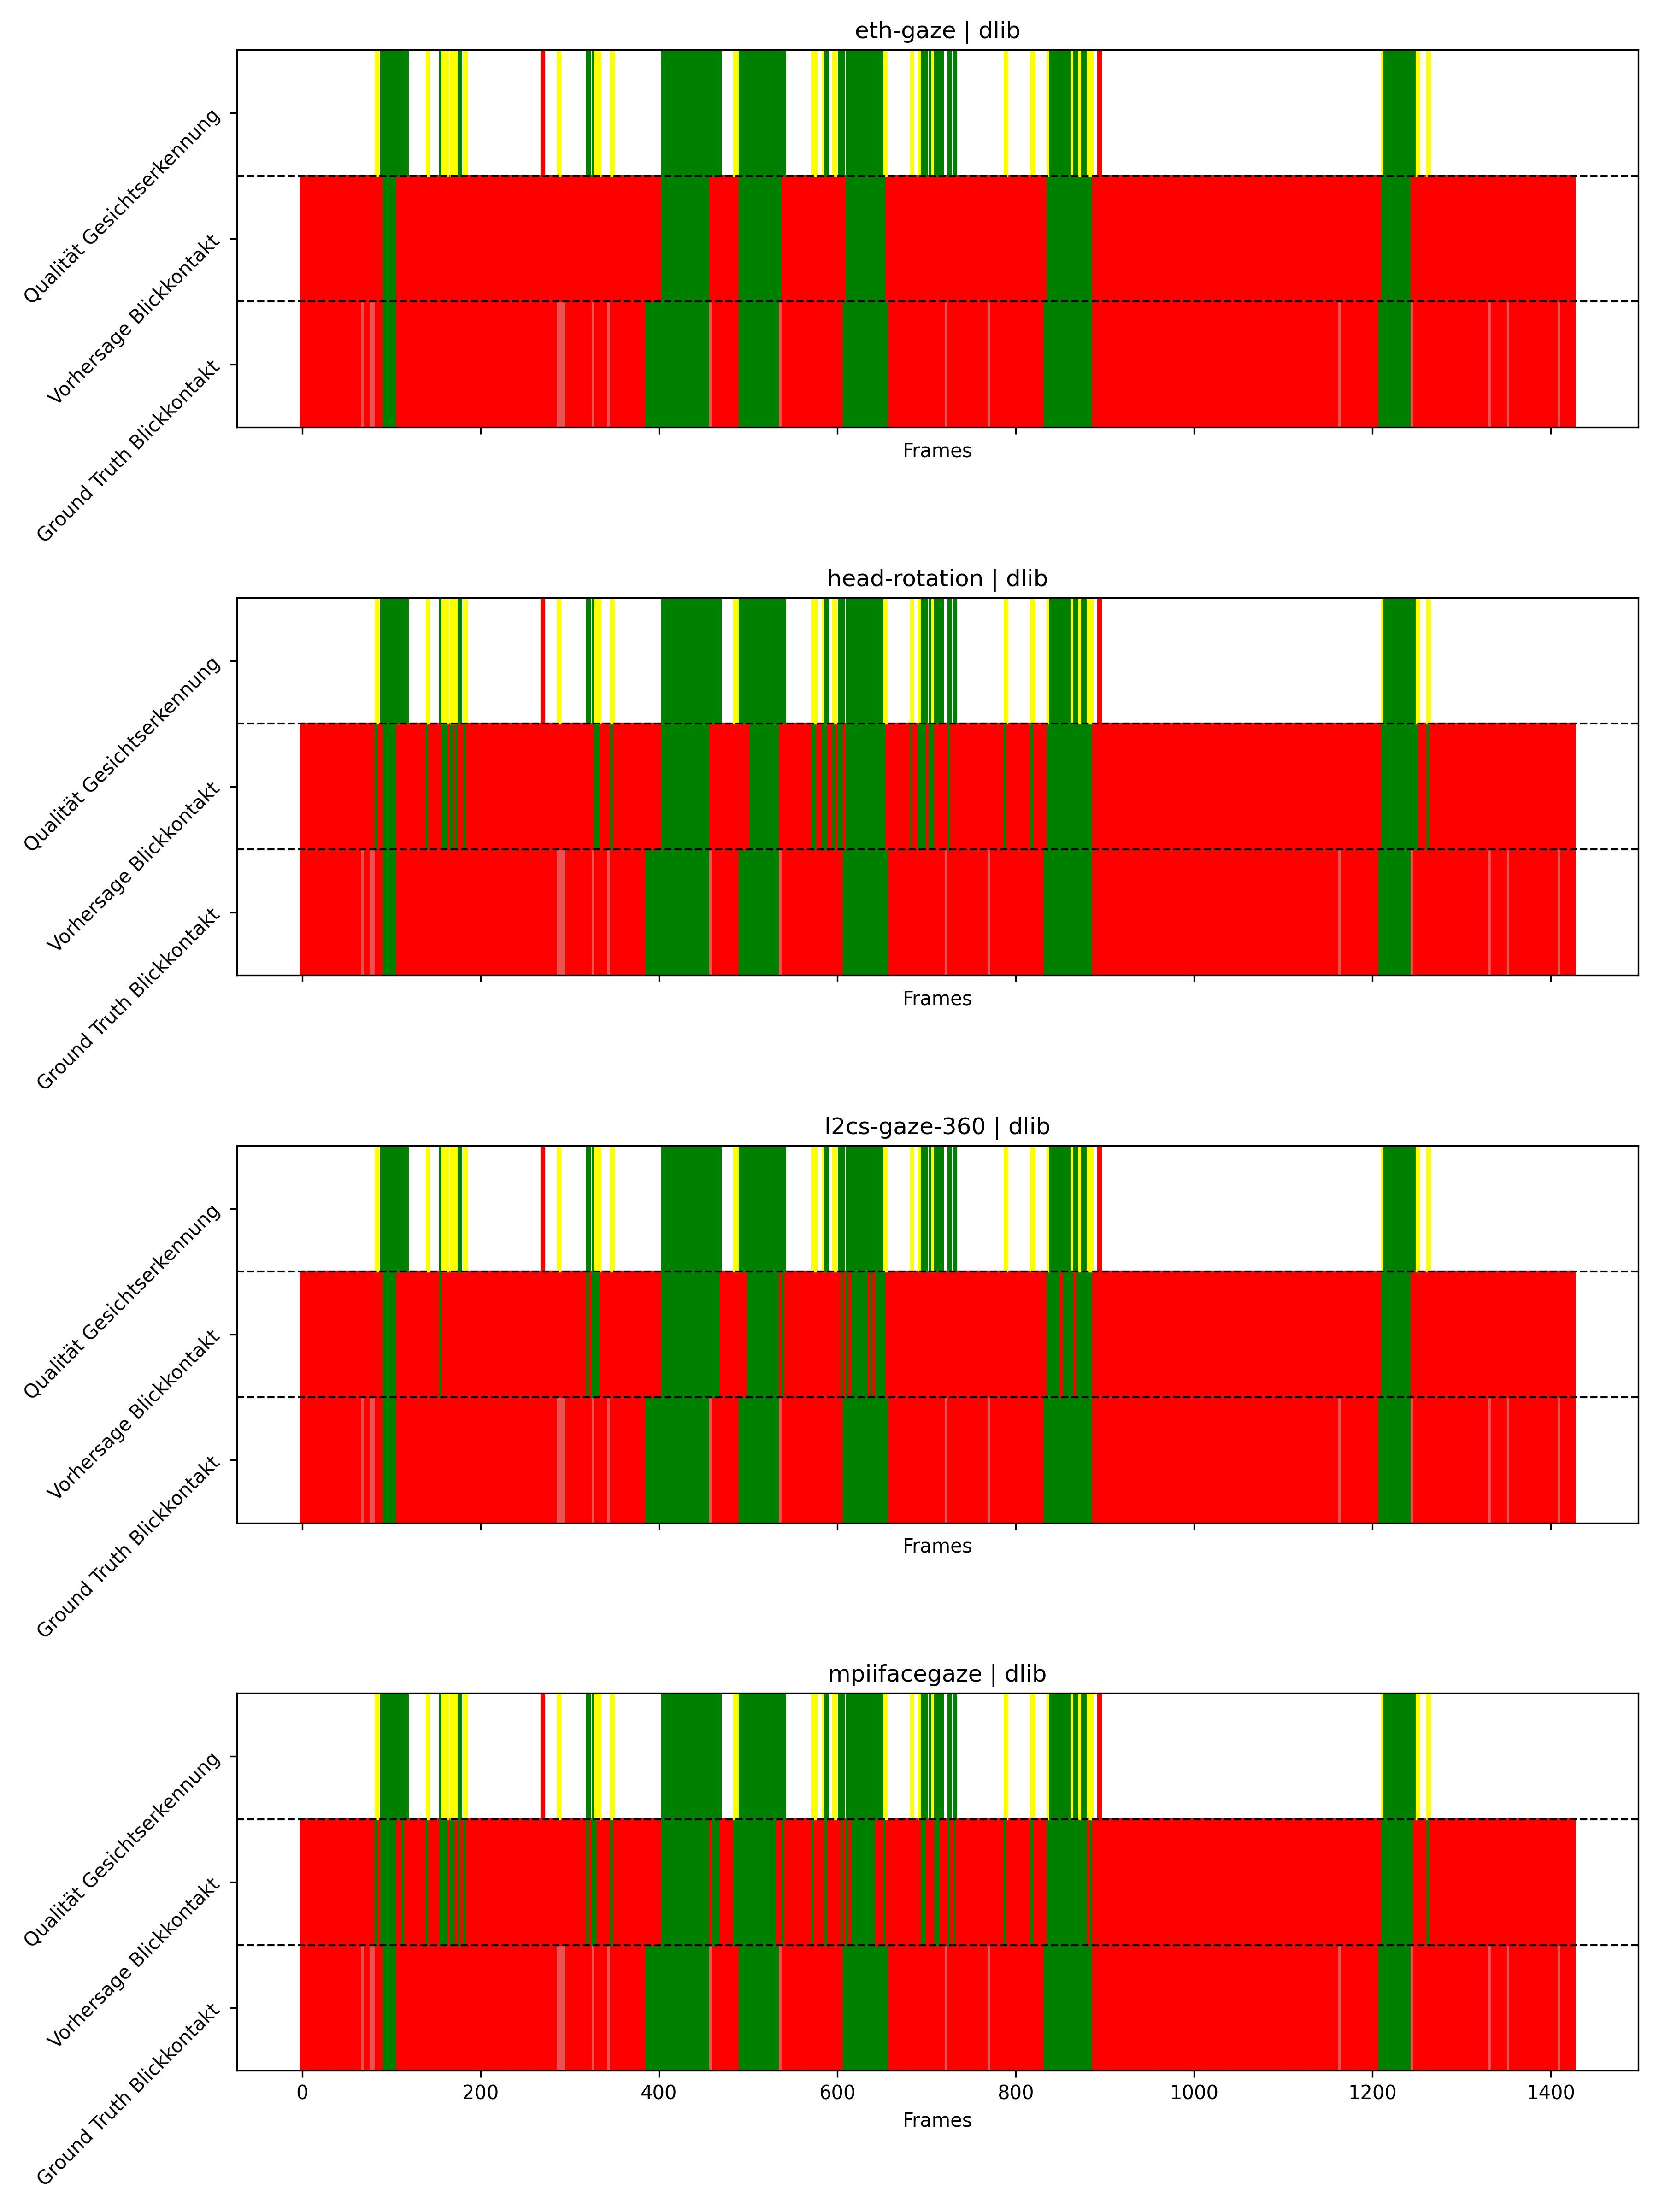
\includegraphics[width=1\linewidth]{appendix/05-dlib-overview-gaze.jpg}
\caption{Überblick über die Ground Truth des Blickkontakts, die Vorhersage des Blickkontakts und die Qualität der Gesichtserkennung mit \dlib. Die Bedeutung der Farben ist in Abbildung \ref{fig:evaluation:gaze:mpiifacegaze} erklärt.  }
\end{figure}

\begin{figure}[H]
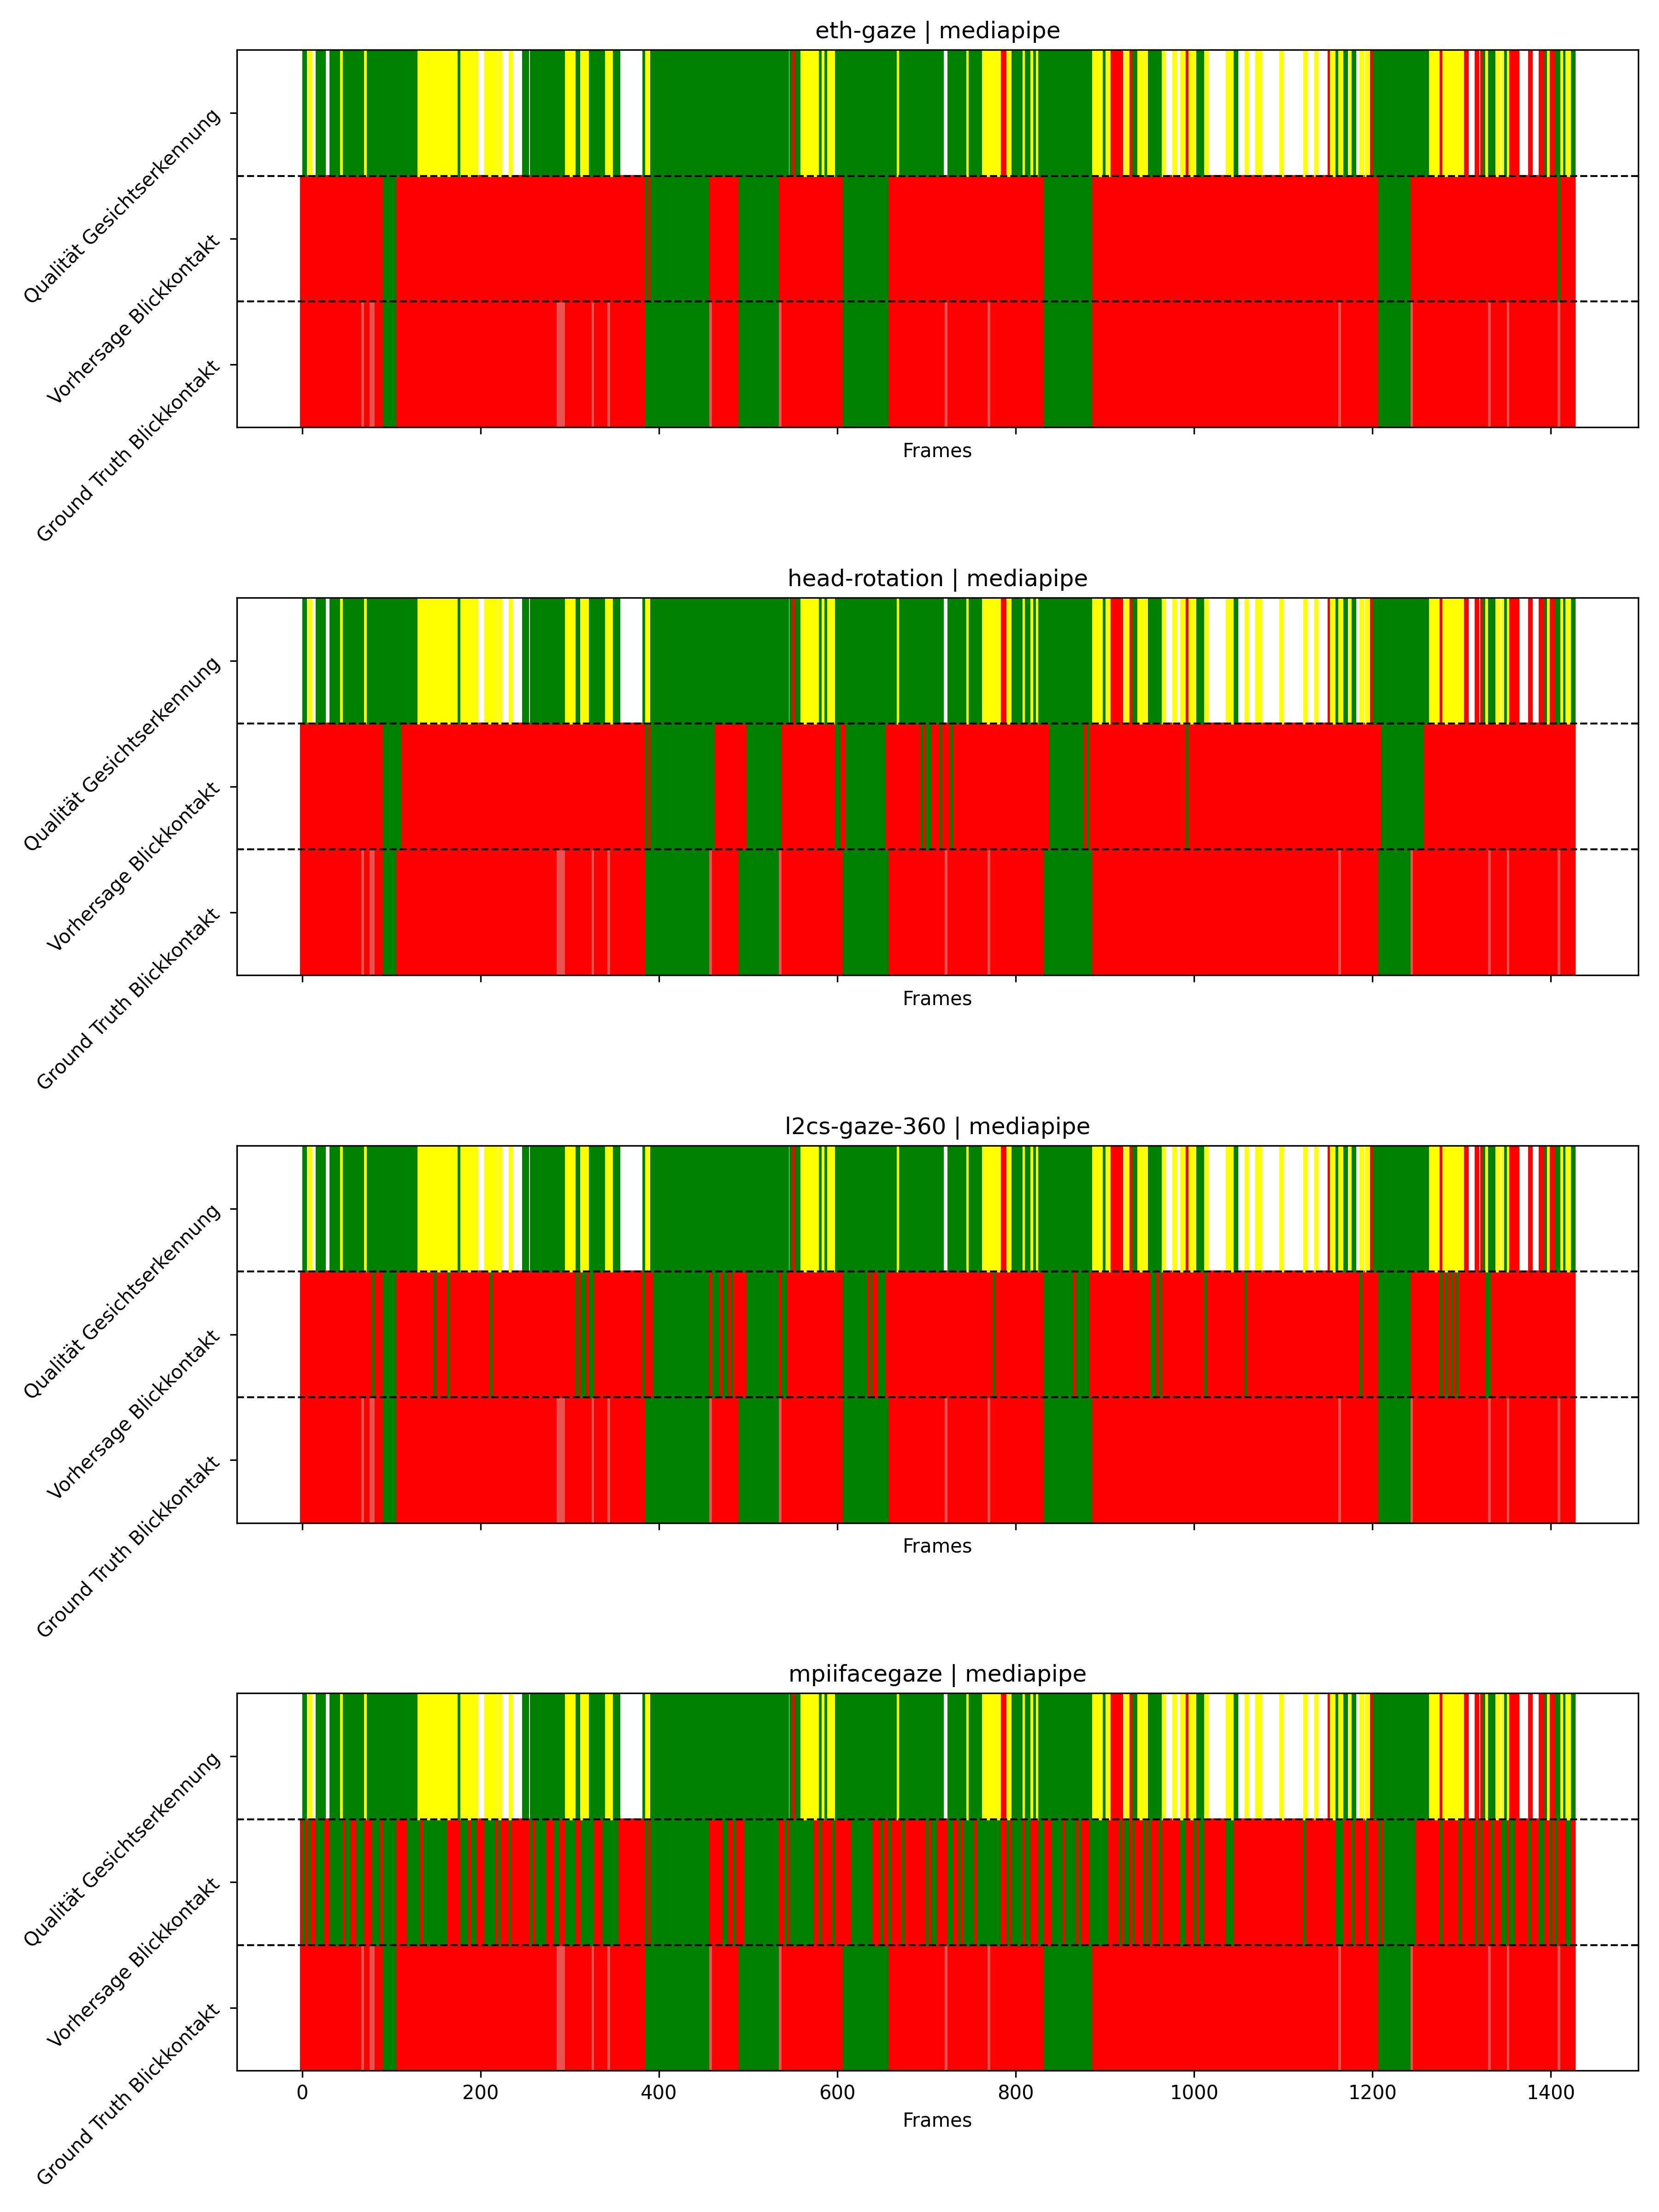
\includegraphics[width=1\linewidth]{appendix/05-mediapipe-overview-gaze.jpg}
\caption{Überblick über die Ground Truth des Blickkontakts, die Vorhersage des Blickkontakts und die Qualität der Gesichtserkennung mit \mediapipe. Die Bedeutung der Farben ist in Abbildung \ref{fig:evaluation:gaze:mpiifacegaze} erklärt.}
\end{figure}

\section{Video 06}
\begin{figure}[H]
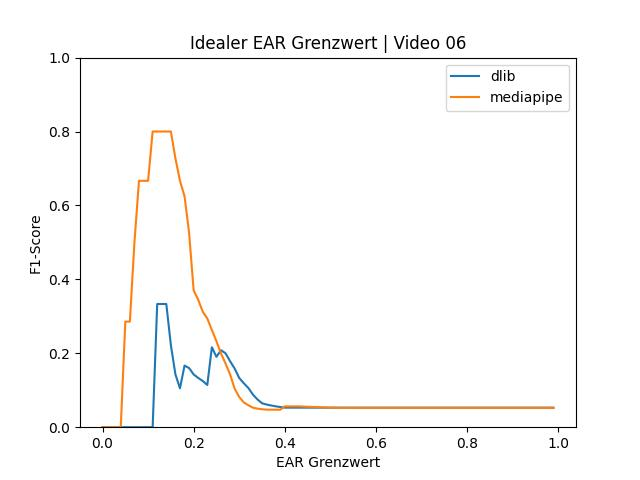
\includegraphics[width=0.7\linewidth]{appendix/06_f1-score-blink.jpg}
\caption{Ergebnisse der Bestimmung des idealen EAR-Grenzwerts für Video 06.}
\end{figure}

\begin{figure}[H]
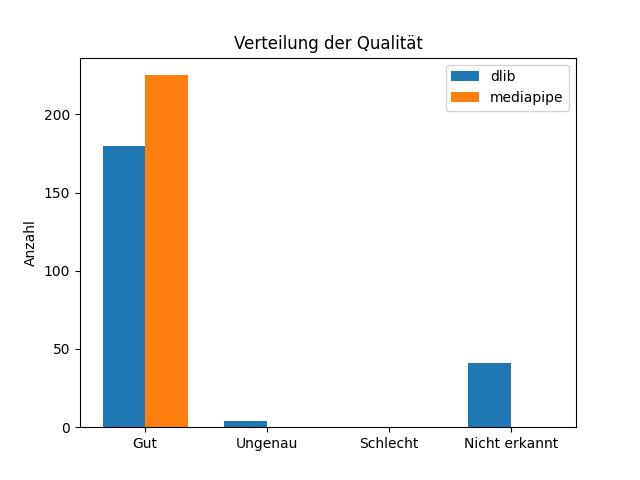
\includegraphics[width=0.7\linewidth]{appendix/06_bar-quality.jpg}
\caption{Aufteilung der Gesichtserkennungsqualität von Video 06.}
\end{figure}

\begin{table}[H]
\centering
\begin{tabular}{l|l|c c |c}
\toprule
\textbf{Gesichtserkennung} & \textbf{Blickrichtung} & \textbf{Seitenlänge} $\hitthresholdsize$ & \textbf{Verschiebung} $\hitthresholdposition$ & \textbf{F1-Score} \\ 
\midrule
\multirow{4}*{dlib}& ETH-XGaze & 0,092 & -0,027 & 0,991  \\ 
& Gaze360 & 0,276 & 0,231 & 0,842 \\ 
& MPIIFaceGaze & 0,041 & -0,027 & 0,831  \\ 
& Kopfrotation & 0,112 & 0,108 & 0,573  \\ 
\hline\multirow{4}*{MediaPipe}& ETH-XGaze & 0,173 & 0,01 & 0,982  \\ 
& Gaze360 & 0,133 & 0,047 & 0,876 \\ 
& MPIIFaceGaze & 0,041 & -0,027 & 0,895  \\ 
& Kopfrotation & 0,112 & 0,12 & 0,568  \\ 
\bottomrule\end{tabular}
\caption{Ergebnis des Hyperparameter-Tunings für die Zone speziell für Video 06.}
\label{tab:appendix:06:local}
\end{table}
\begin{table}[H]
\centering
\begin{tabular}{l|l|c c c c|c c|c}
\toprule
\textbf{Gesichtserkennung} & \textbf{Blickrichtung} & $TP$ & $TN$& $FP$ & $FN$ & \textbf{Precision} & \textbf{Recall} & \textbf{F1-Score} \\ 
\midrule
\multirow{4}*{dlib}& ETH-XGaze & 55 & 158 & 12 & 0 & 0,821 & 1,0 & 0,902 \\ 
& Gaze360 & 53 & 107 & 63 & 2 & 0,457 & 0,964 & 0,62 \\ 
& MPIIFaceGaze & 55 & 104 & 66 & 0 & 0,455 & 1,0 & 0,625 \\ 
& Kopfrotation & 55 & 59 & 111 & 0 & 0,331 & 1,0 & 0,498 \\ 
\hline\multirow{4}*{MediaPipe}& ETH-XGaze & 55 & 138 & 32 & 0 & 0,632 & 1,0 & 0,775 \\ 
& Gaze360 & 53 & 126 & 44 & 2 & 0,546 & 0,964 & 0,697 \\ 
& MPIIFaceGaze & 55 & 153 & 17 & 0 & 0,764 & 1,0 & 0,866 \\ 
& Kopfrotation & 55 & 60 & 110 & 0 & 0,333 & 1,0 & 0,5 \\ 
\bottomrule\end{tabular}
\caption{Zusammensetzung des F1-Scores unter Verwendung der in Kapitel \ref{sec:evaluation:results:gaze:threshold} bestimmten globalen Parameter $\hitthresholdsize$ und $\hitthresholdposition$.}
\label{tab:appendix:06:f1}
\end{table}
\begin{figure}[H]
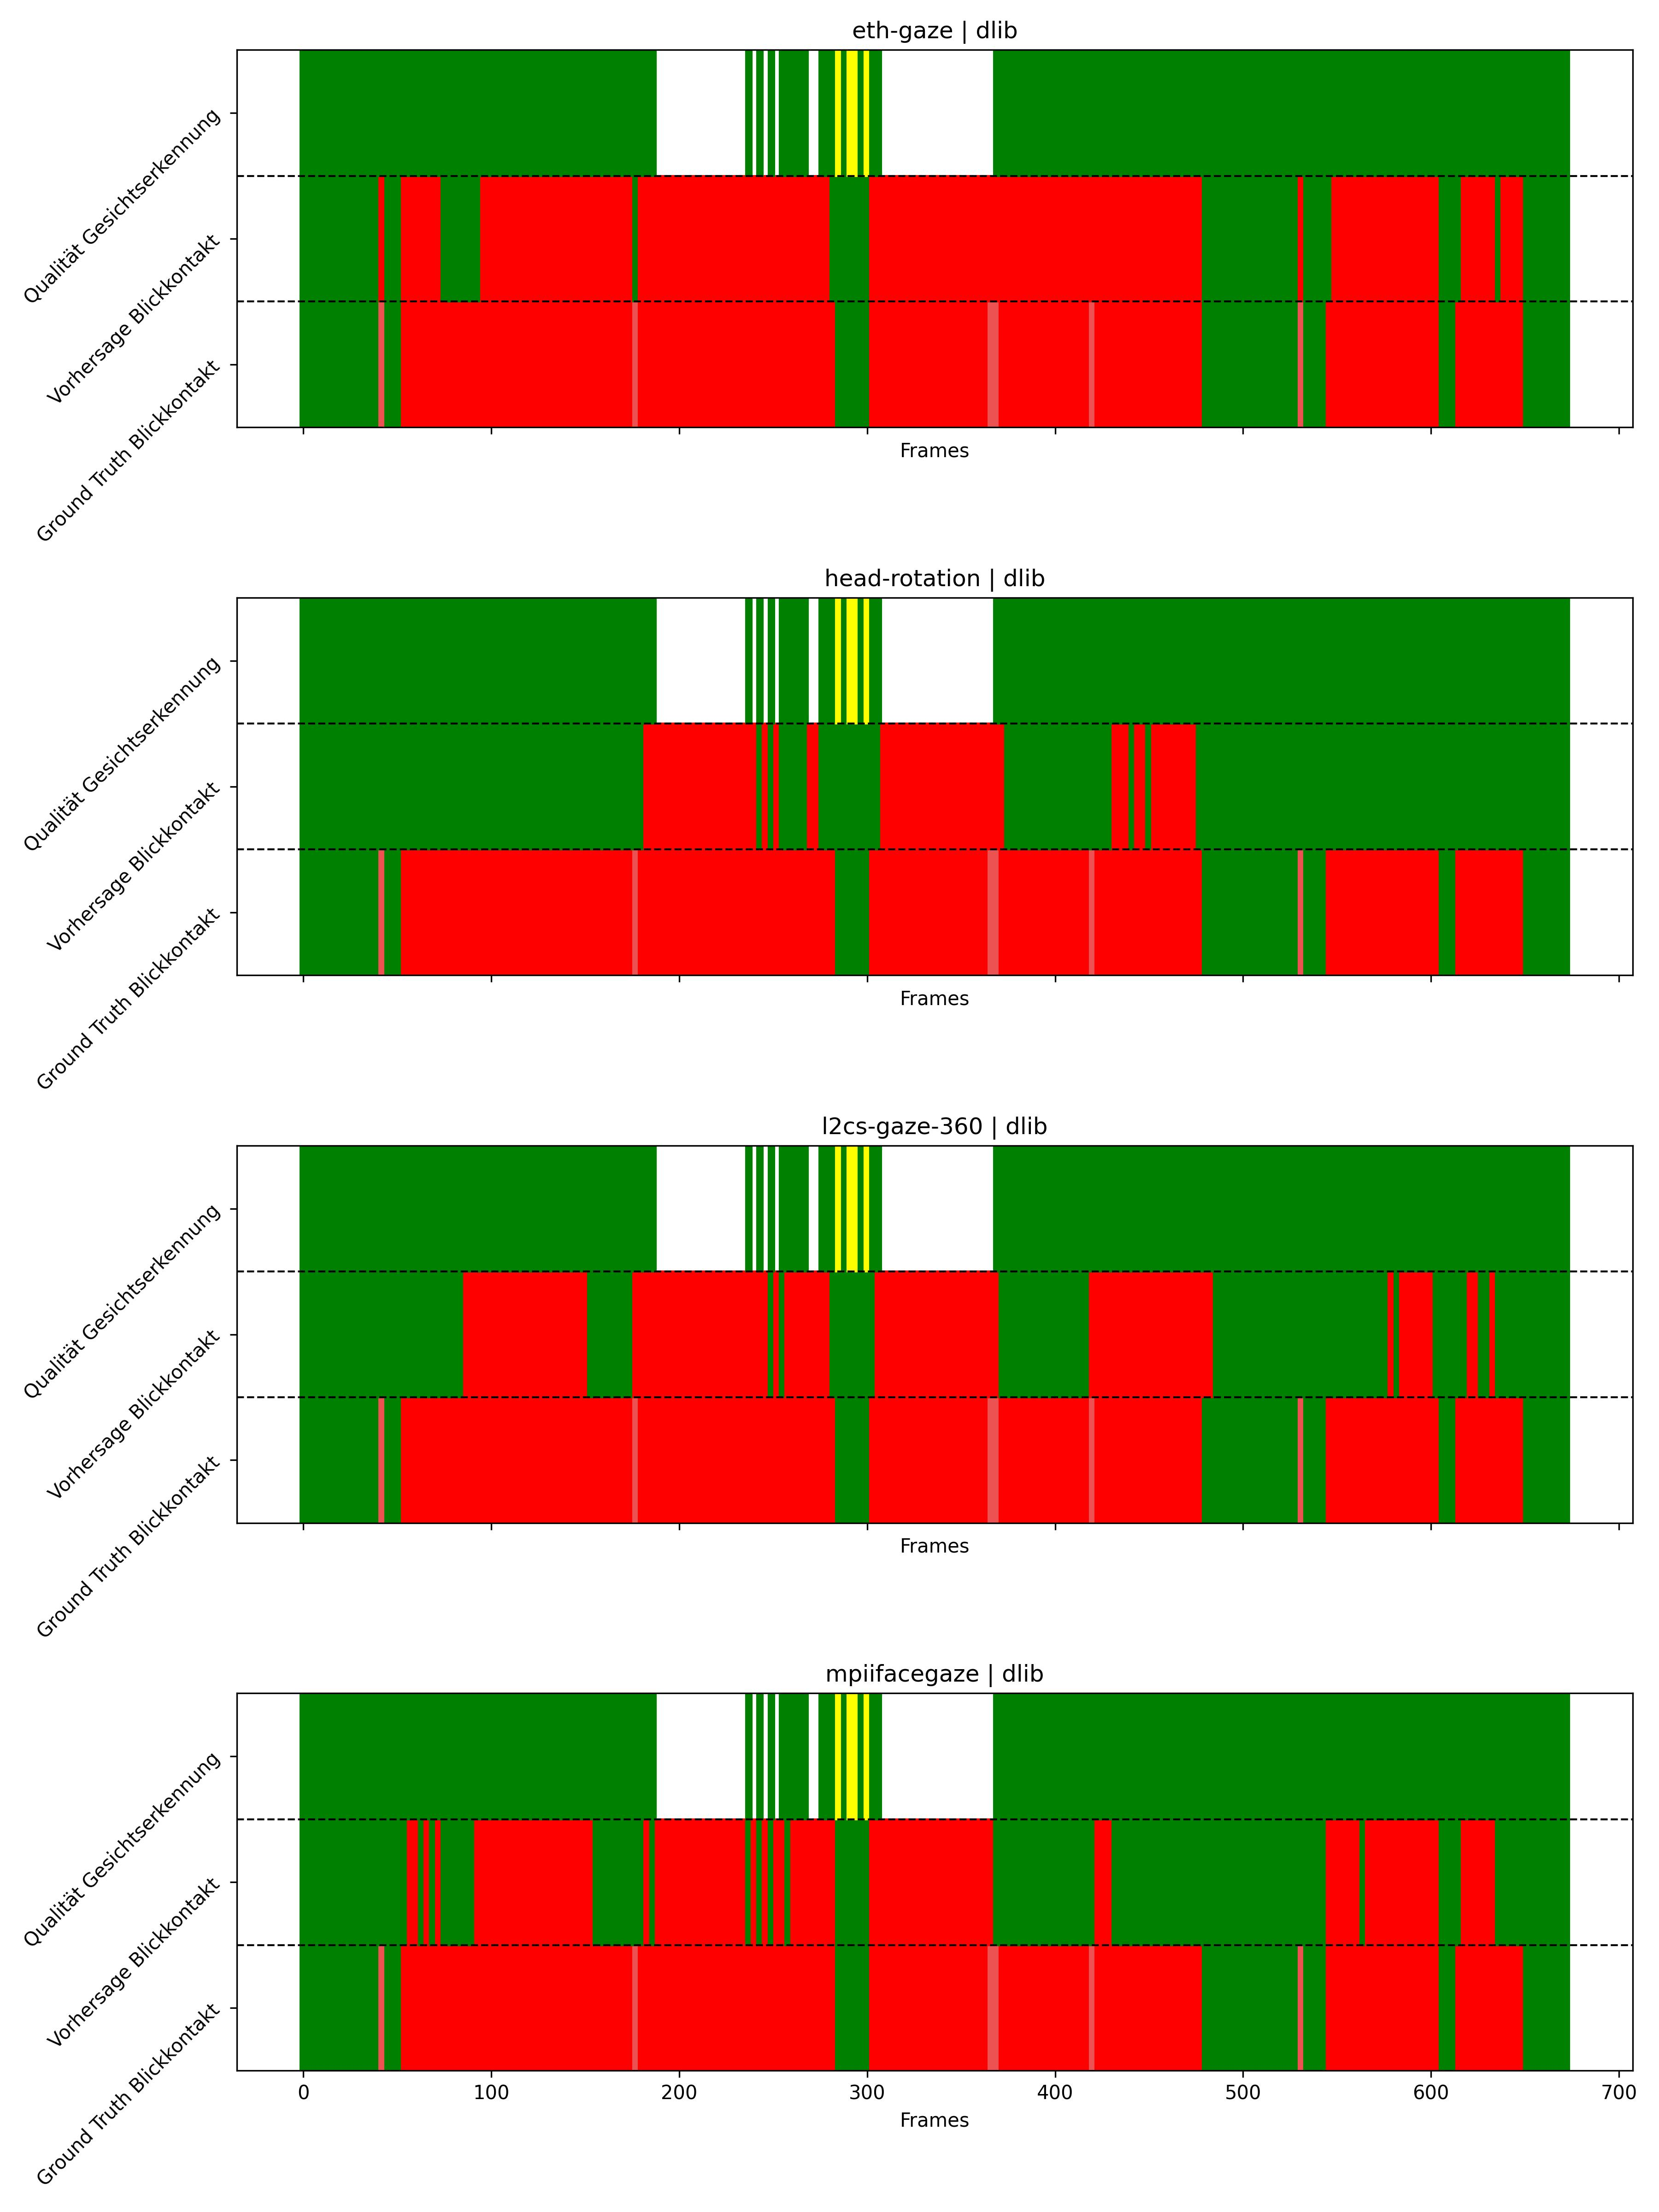
\includegraphics[width=1\linewidth]{appendix/06-dlib-overview-gaze.jpg}
\caption{Überblick über die Ground Truth des Blickkontakts, die Vorhersage des Blickkontakts und die Qualität der Gesichtserkennung mit \dlib. Die Bedeutung der Farben ist in Abbildung \ref{fig:evaluation:gaze:mpiifacegaze} erklärt.  }
\end{figure}

\begin{figure}[H]
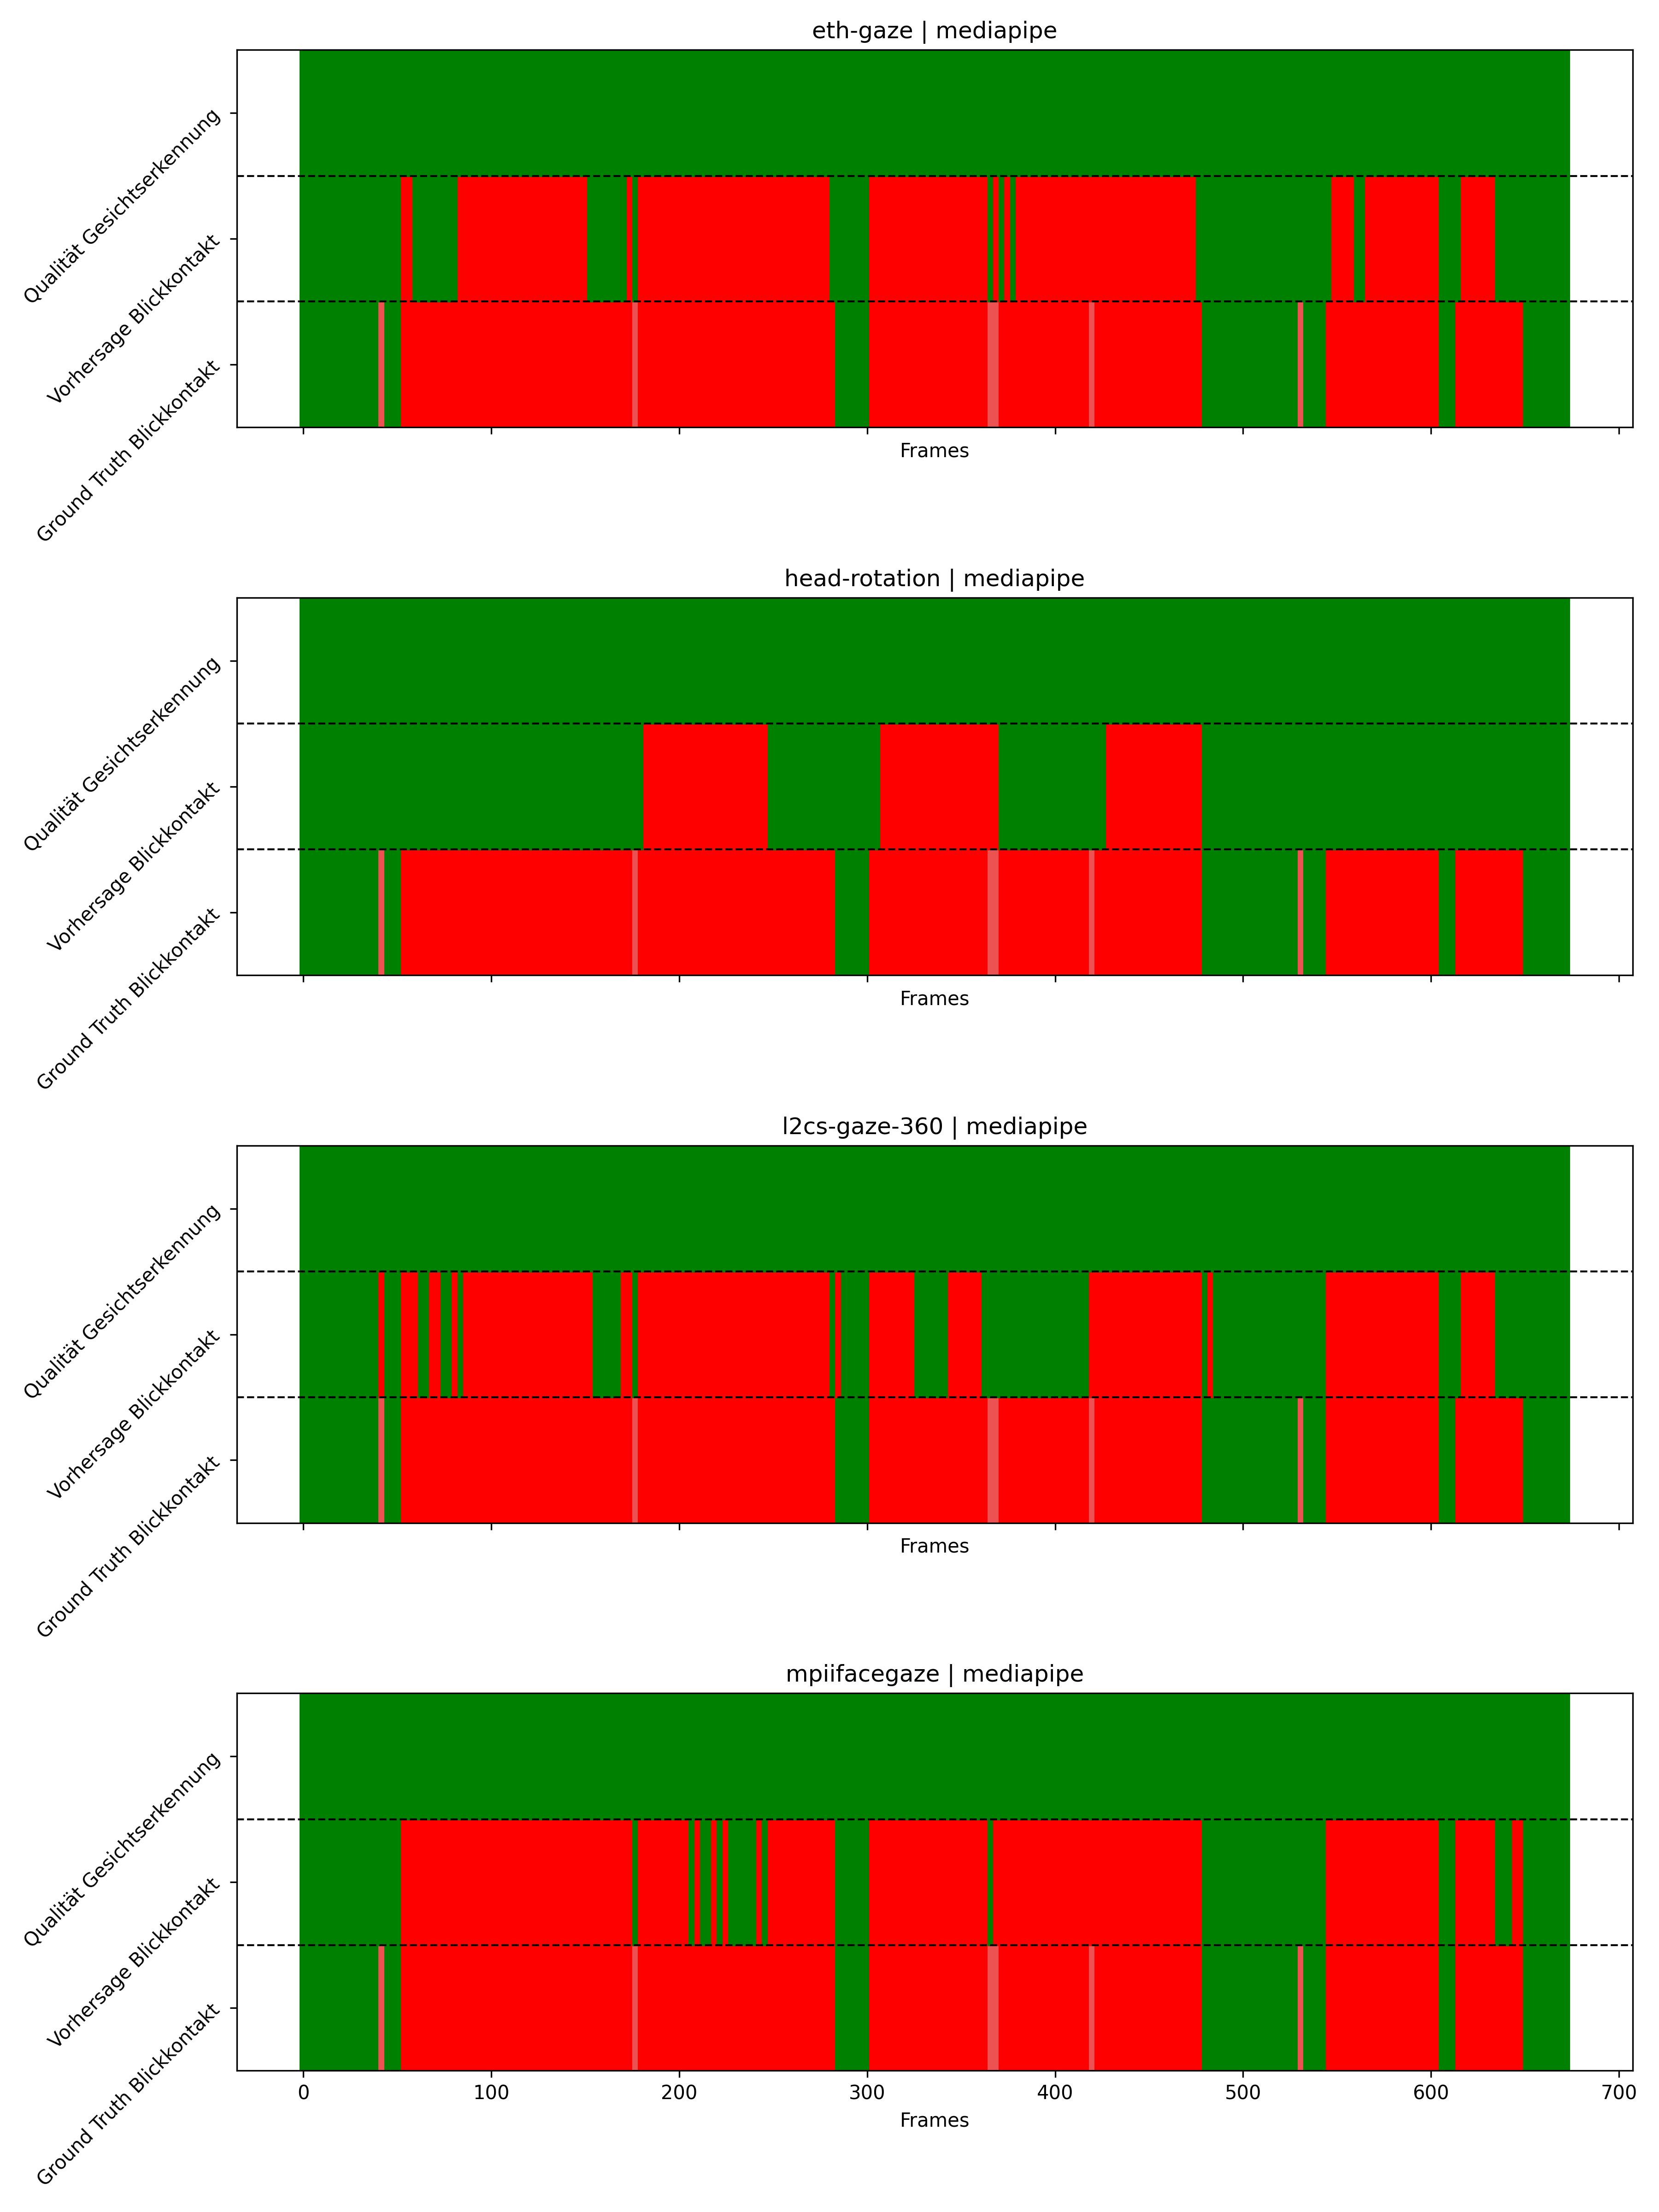
\includegraphics[width=1\linewidth]{appendix/06-mediapipe-overview-gaze.jpg}
\caption{Überblick über die Ground Truth des Blickkontakts, die Vorhersage des Blickkontakts und die Qualität der Gesichtserkennung mit \mediapipe. Die Bedeutung der Farben ist in Abbildung \ref{fig:evaluation:gaze:mpiifacegaze} erklärt.}
\end{figure}

\section{Video 07}
\begin{figure}[H]
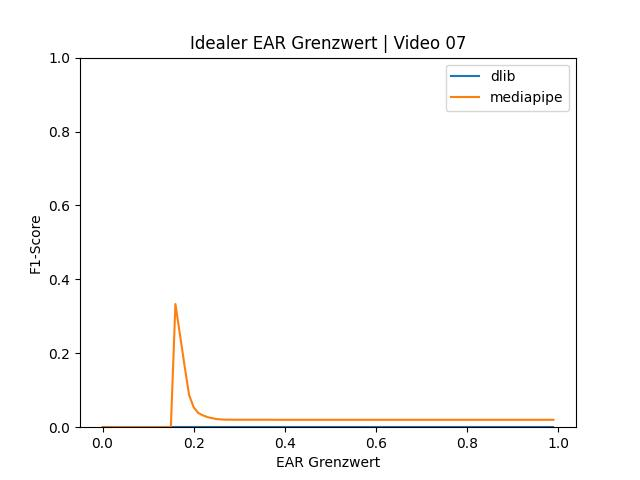
\includegraphics[width=0.7\linewidth]{appendix/07_f1-score-blink.jpg}
\caption{Ergebnisse der Bestimmung des idealen EAR-Grenzwerts für Video 07.}
\end{figure}

\begin{figure}[H]
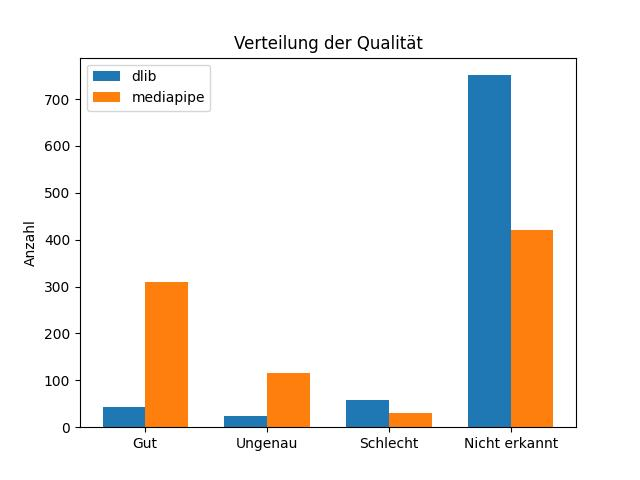
\includegraphics[width=0.7\linewidth]{appendix/07_bar-quality.jpg}
\caption{Aufteilung der Gesichtserkennungsqualität von Video 07.}
\end{figure}

\begin{table}[H]
\centering
\begin{tabular}{l|l|c c |c}
\toprule
\textbf{Gesichtserkennung} & \textbf{Blickrichtung} & \textbf{Seitenlänge} $\hitthresholdsize$ & \textbf{Verschiebung} $\hitthresholdposition$ & \textbf{F1-Score} \\ 
\midrule
\multirow{4}*{dlib}& ETH-XGaze & 0,357 & 0,059 & 0,626  \\ 
& Gaze360 & 0,5 & 0,084 & 0,435 \\ 
& MPIIFaceGaze & 0,102 & 0,035 & 0,581  \\ 
& Kopfrotation & 0,235 & 0,292 & 0,575  \\ 
\hline\multirow{4}*{MediaPipe}& ETH-XGaze & 0,296 & 0,084 & 0,786  \\ 
& Gaze360 & 0,5 & 0,071 & 0,4 \\ 
& MPIIFaceGaze & 0,112 & 0,059 & 0,788  \\ 
& Kopfrotation & 0,184 & 0,292 & 0,9  \\ 
\bottomrule\end{tabular}
\caption{Ergebnis des Hyperparameter-Tunings für die Zone speziell für Video 07.}
\label{tab:appendix:07:local}
\end{table}
\begin{table}[H]
\centering
\begin{tabular}{l|l|c c c c|c c|c}
\toprule
\textbf{Gesichtserkennung} & \textbf{Blickrichtung} & $TP$ & $TN$& $FP$ & $FN$ & \textbf{Precision} & \textbf{Recall} & \textbf{F1-Score} \\ 
\midrule
\multirow{4}*{dlib}& ETH-XGaze & 25 & 758 & 4 & 88 & 0,862 & 0,221 & 0,352 \\ 
& Gaze360 & 30 & 742 & 20 & 83 & 0,6 & 0,265 & 0,368 \\ 
& MPIIFaceGaze & 42 & 712 & 50 & 71 & 0,457 & 0,372 & 0,41 \\ 
& Kopfrotation & 35 & 717 & 45 & 78 & 0,438 & 0,31 & 0,363 \\ 
\hline\multirow{4}*{MediaPipe}& ETH-XGaze & 56 & 736 & 26 & 57 & 0,683 & 0,496 & 0,574 \\ 
& Gaze360 & 46 & 638 & 124 & 67 & 0,271 & 0,407 & 0,325 \\ 
& MPIIFaceGaze & 56 & 671 & 91 & 57 & 0,381 & 0,496 & 0,431 \\ 
& Kopfrotation & 33 & 762 & 0 & 80 & 1,0 & 0,292 & 0,452 \\ 
\bottomrule\end{tabular}
\caption{Zusammensetzung des F1-Scores unter Verwendung der in Kapitel \ref{sec:evaluation:results:gaze:threshold} bestimmten globalen Parameter $\hitthresholdsize$ und $\hitthresholdposition$.}
\label{tab:appendix:07:f1}
\end{table}
\begin{figure}[H]
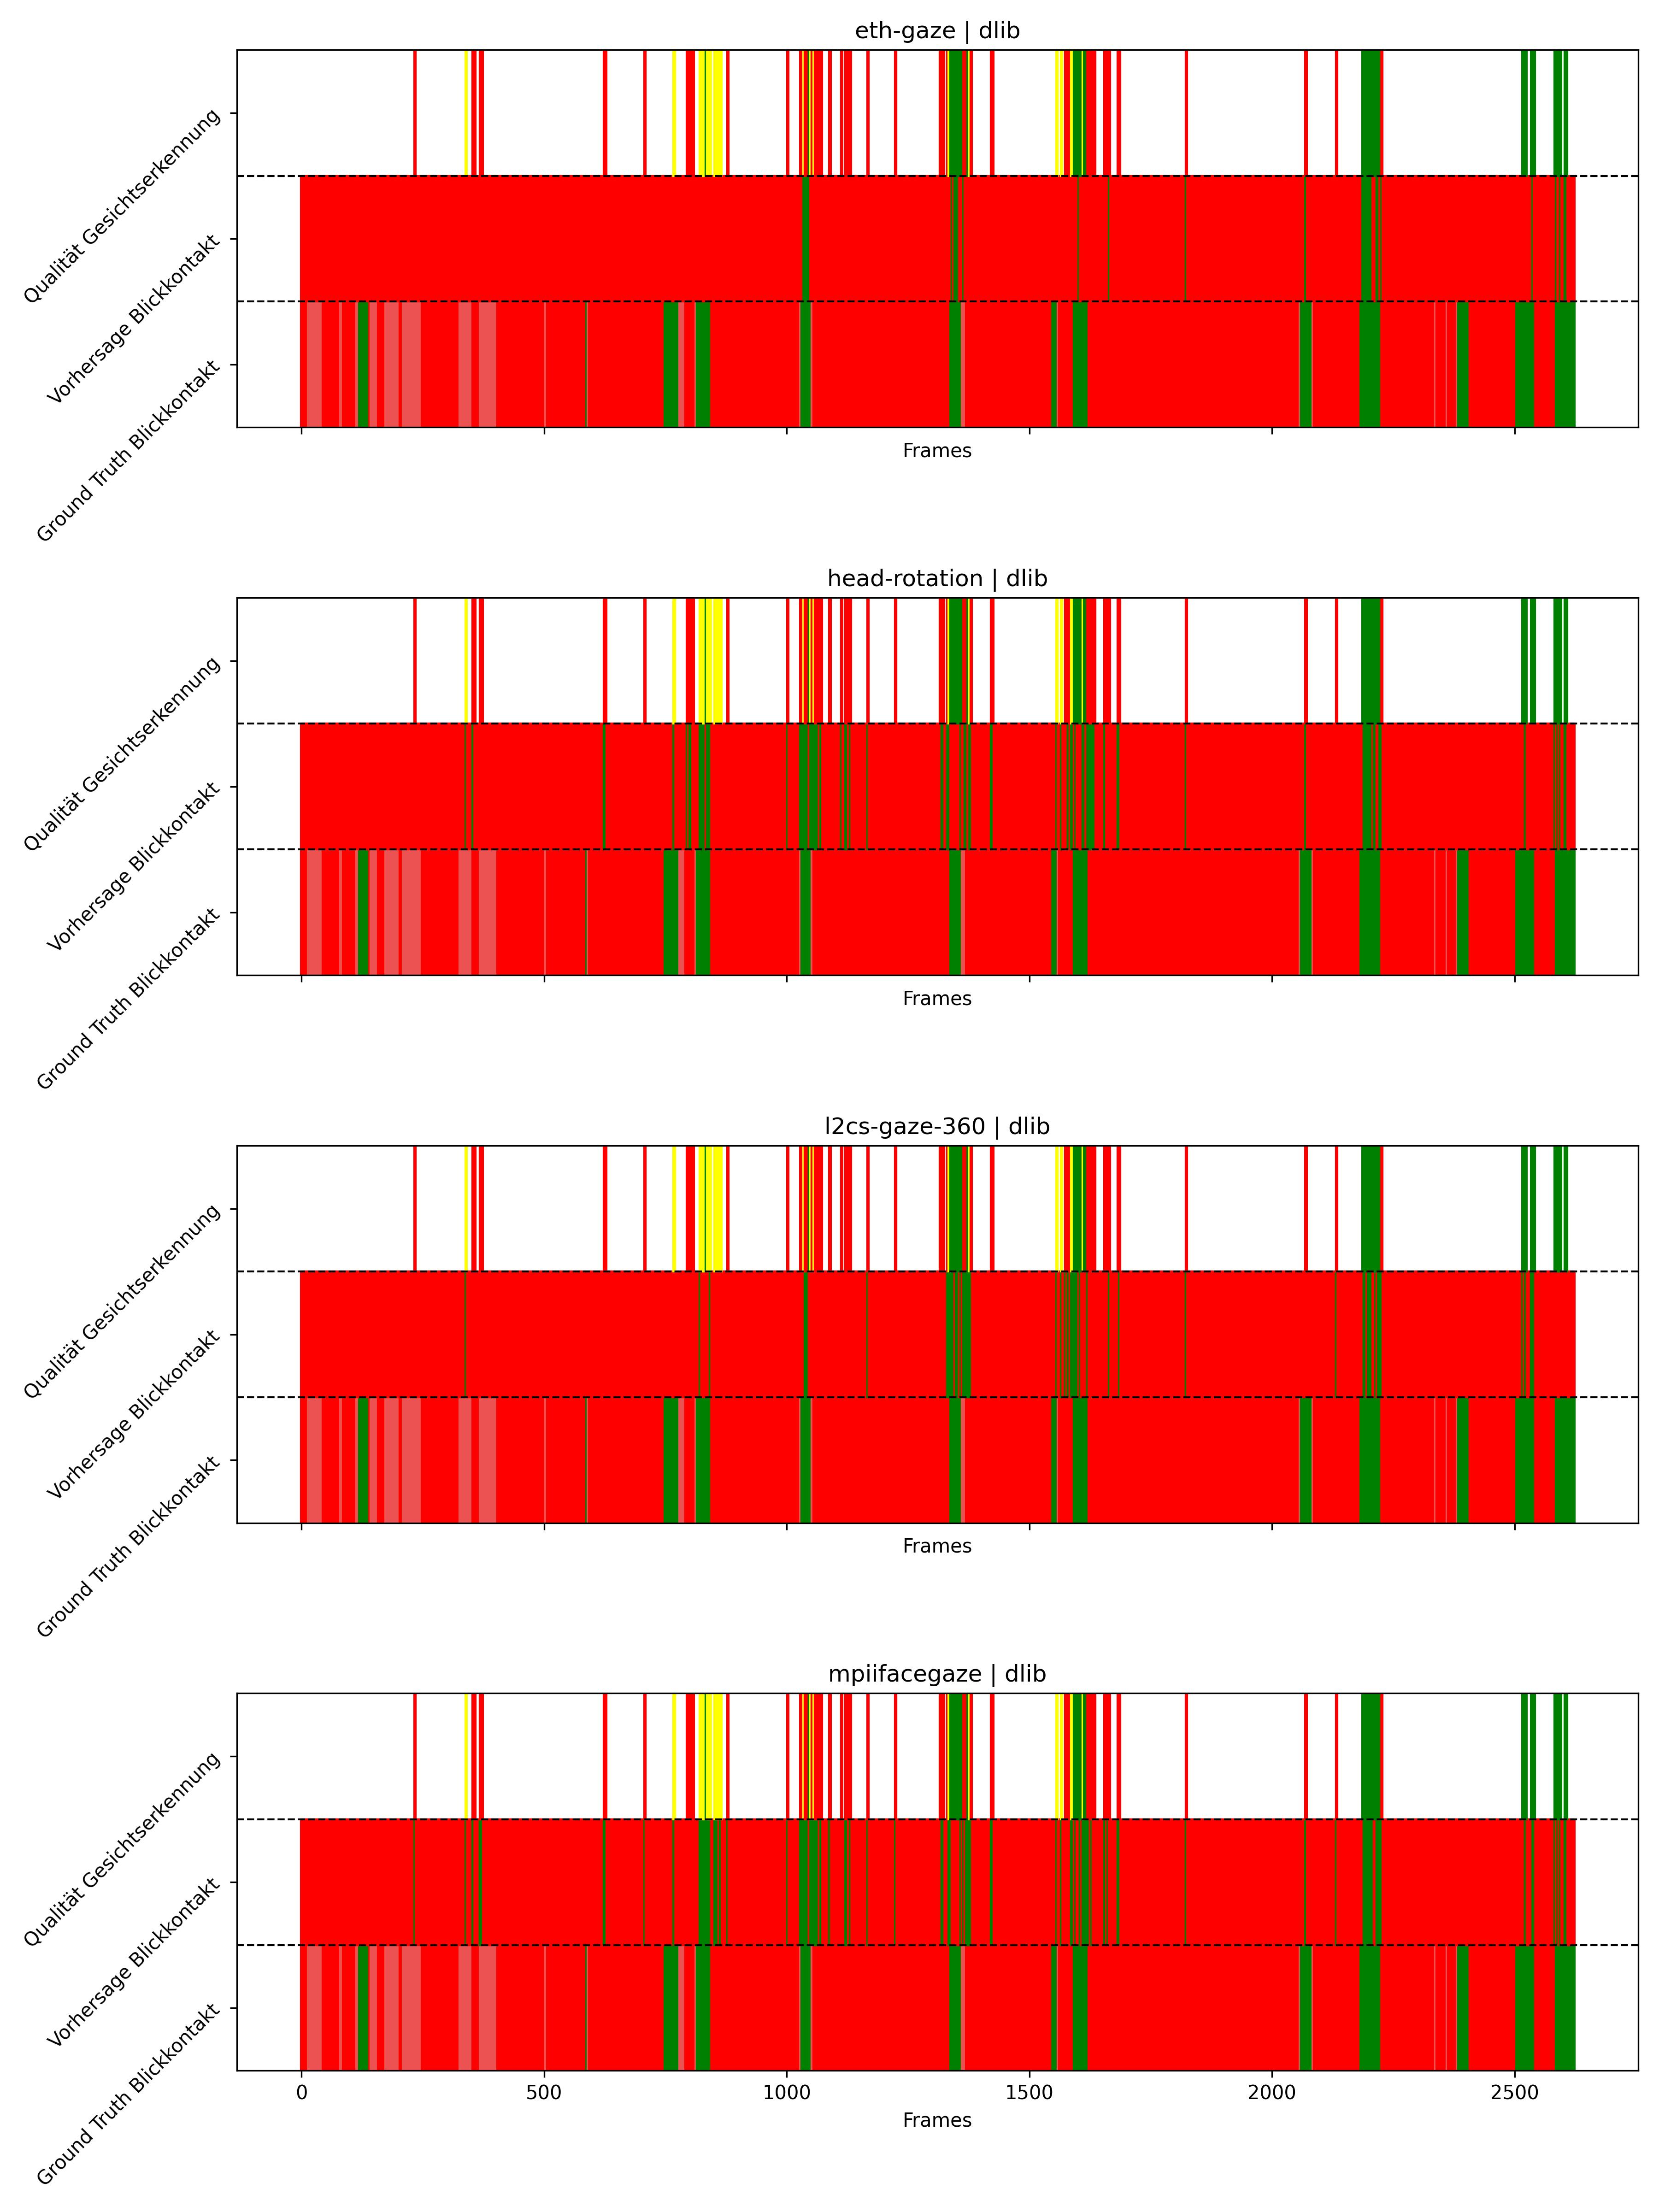
\includegraphics[width=1\linewidth]{appendix/07-dlib-overview-gaze.jpg}
\caption{Überblick über die Ground Truth des Blickkontakts, die Vorhersage des Blickkontakts und die Qualität der Gesichtserkennung mit \dlib. Die Bedeutung der Farben ist in Abbildung \ref{fig:evaluation:gaze:mpiifacegaze} erklärt.  }
\end{figure}

\begin{figure}[H]
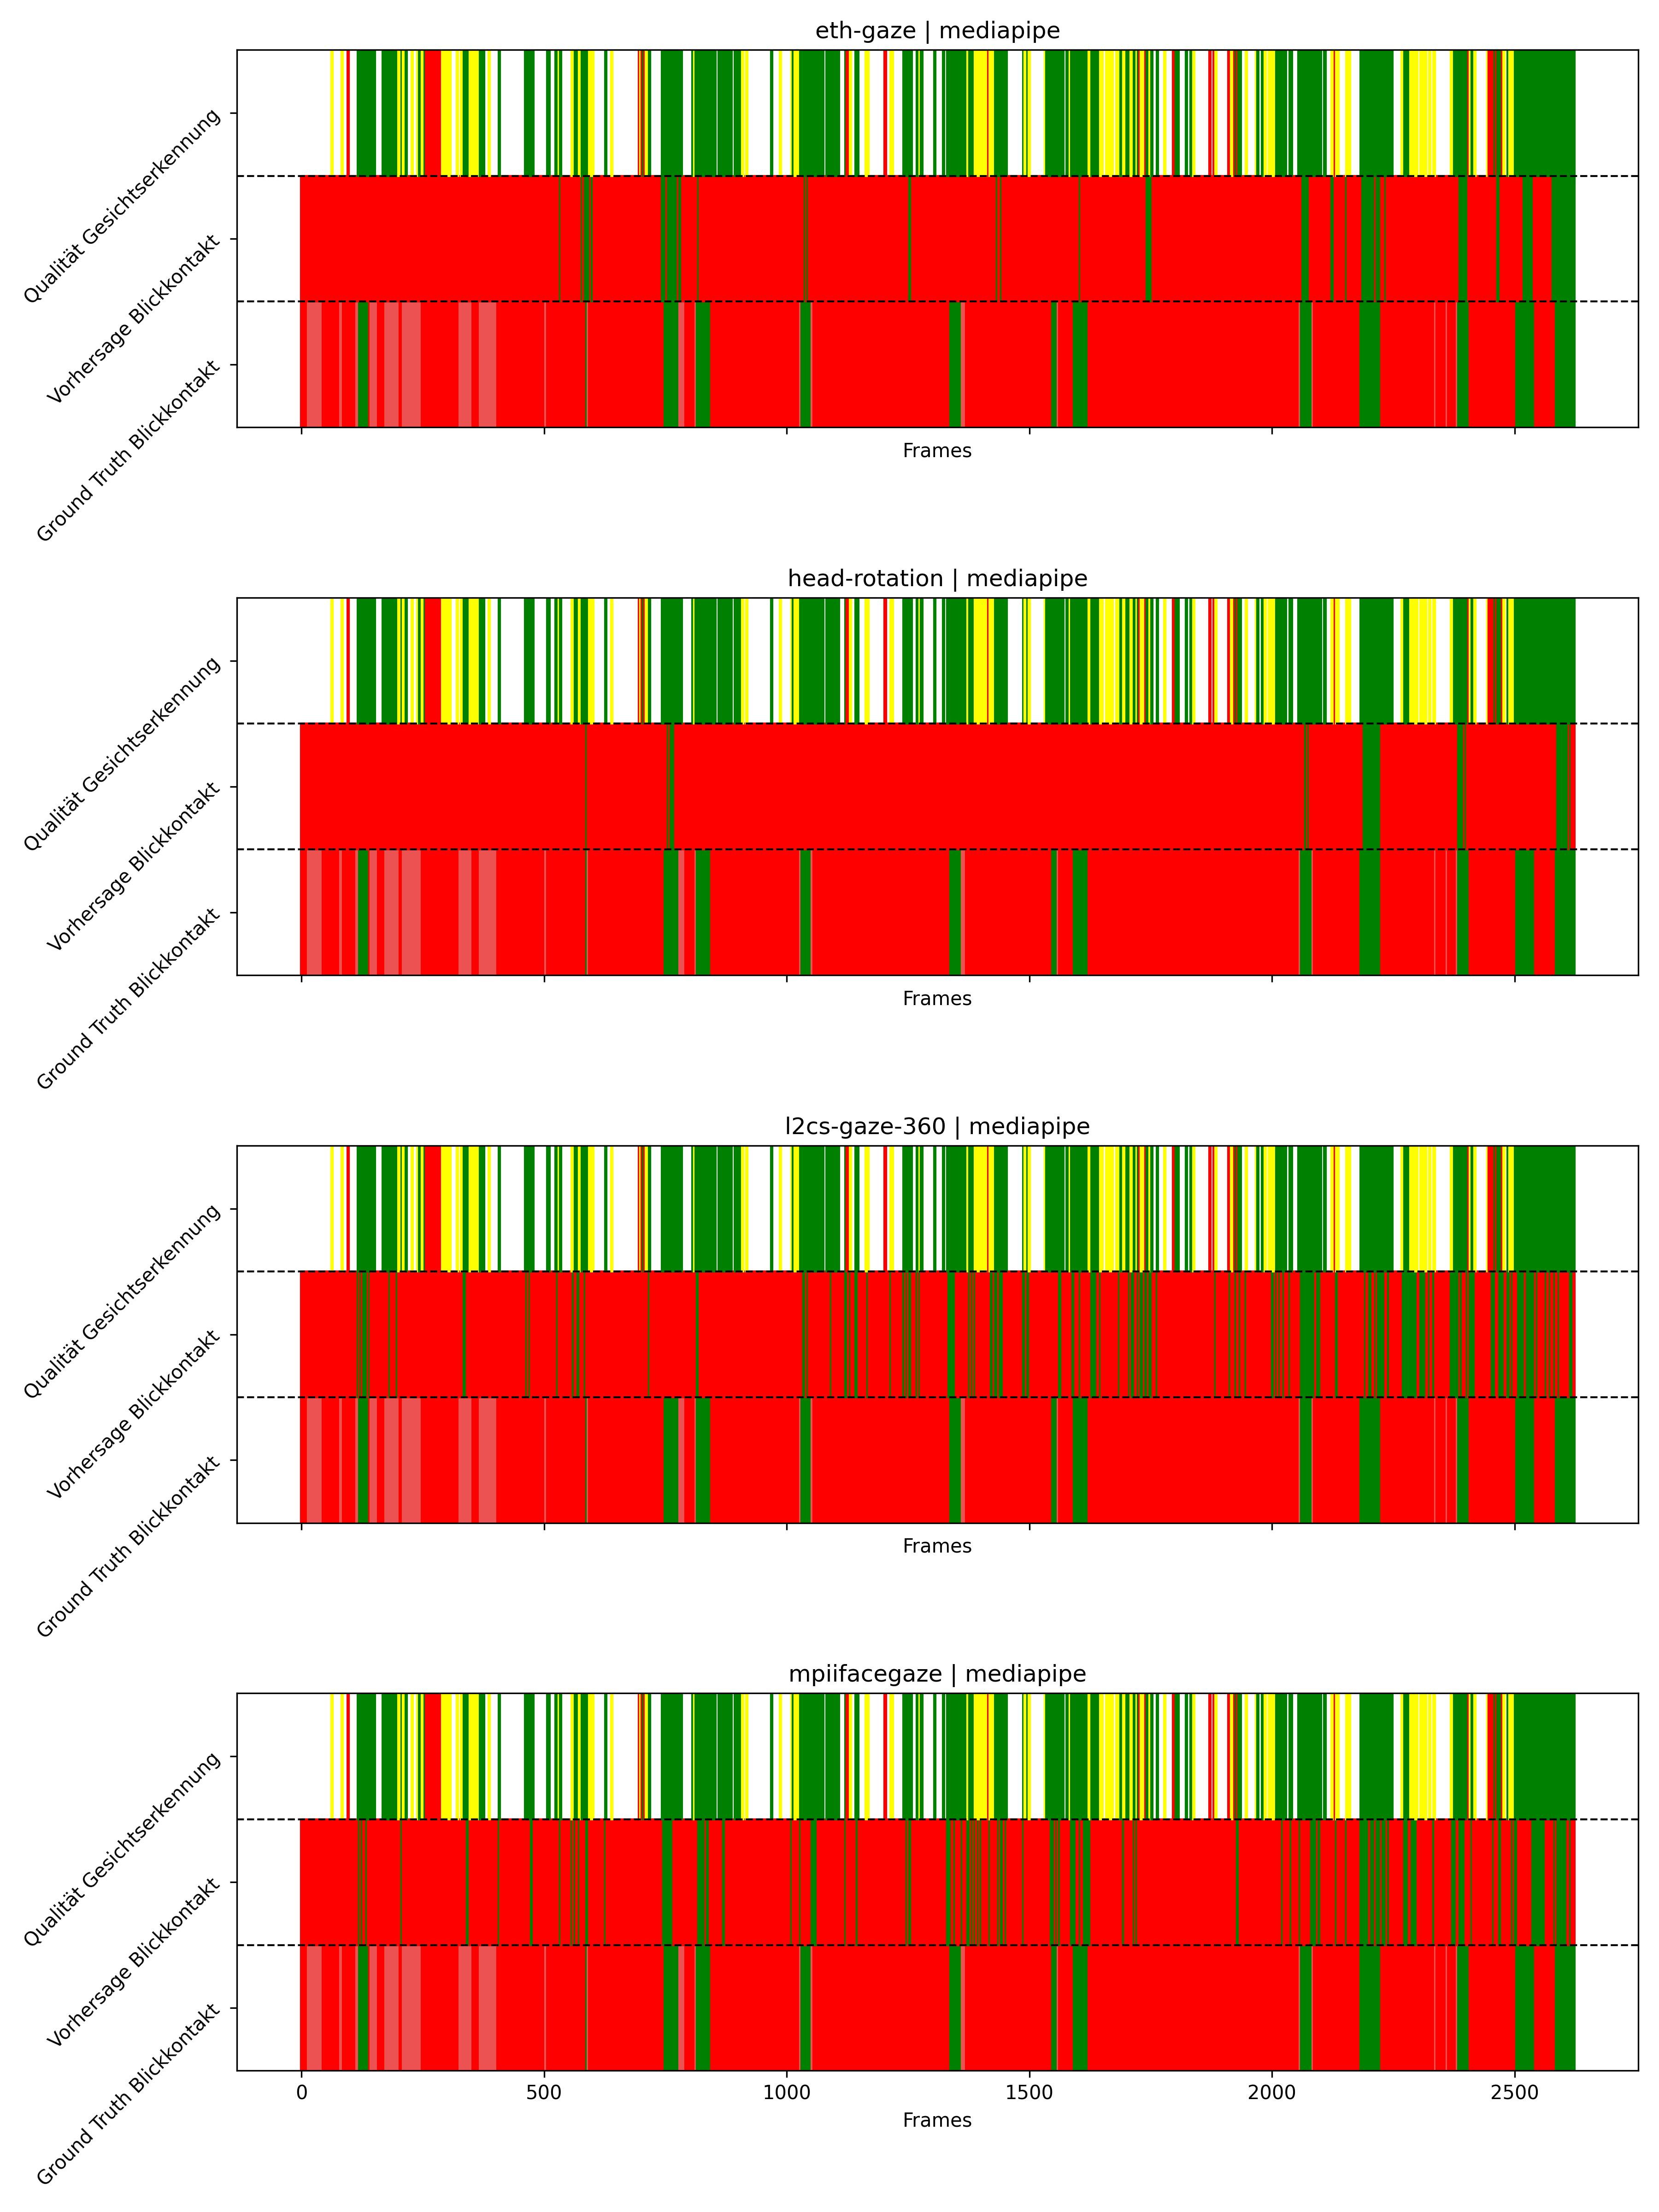
\includegraphics[width=1\linewidth]{appendix/07-mediapipe-overview-gaze.jpg}
\caption{Überblick über die Ground Truth des Blickkontakts, die Vorhersage des Blickkontakts und die Qualität der Gesichtserkennung mit \mediapipe. Die Bedeutung der Farben ist in Abbildung \ref{fig:evaluation:gaze:mpiifacegaze} erklärt.}
\end{figure}

\section{Video 08}
\begin{figure}[H]
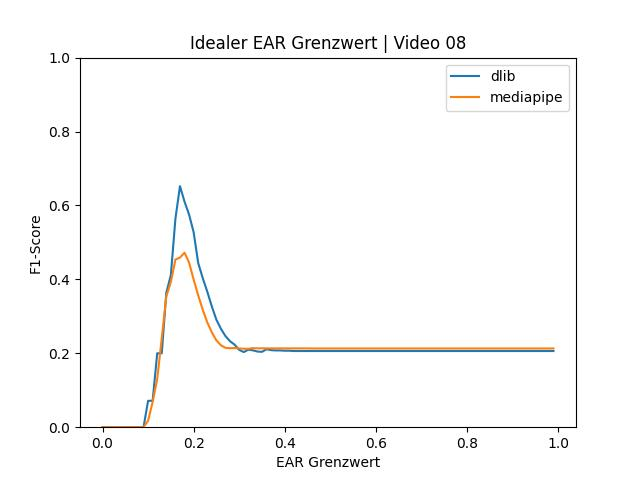
\includegraphics[width=0.7\linewidth]{appendix/08_f1-score-blink.jpg}
\caption{Ergebnisse der Bestimmung des idealen EAR-Grenzwerts für Video 08.}
\end{figure}

\begin{figure}[H]
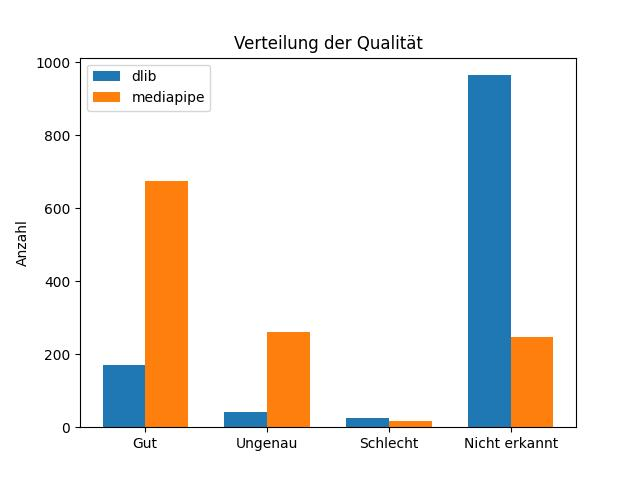
\includegraphics[width=0.7\linewidth]{appendix/08_bar-quality.jpg}
\caption{Aufteilung der Gesichtserkennungsqualität von Video 08.}
\end{figure}

\begin{table}[H]
\centering
\begin{tabular}{l|l|c c |c}
\toprule
\textbf{Gesichtserkennung} & \textbf{Blickrichtung} & \textbf{Seitenlänge} $\hitthresholdsize$ & \textbf{Verschiebung} $\hitthresholdposition$ & \textbf{F1-Score} \\ 
\midrule
\multirow{4}*{dlib}& ETH-XGaze & 0,133 & 0,084 & 0,722  \\ 
& Gaze360 & 0,398 & 0,108 & 0,704 \\ 
& MPIIFaceGaze & 0,041 & 0,01 & 0,516  \\ 
& Kopfrotation & 0,092 & 0,243 & 0,487  \\ 
\hline\multirow{4}*{MediaPipe}& ETH-XGaze & 0,224 & 0,047 & 0,835  \\ 
& Gaze360 & 0,398 & 0,108 & 0,847 \\ 
& MPIIFaceGaze & 0,041 & 0,022 & 0,52  \\ 
& Kopfrotation & 0,102 & 0,231 & 0,667  \\ 
\bottomrule\end{tabular}
\caption{Ergebnis des Hyperparameter-Tunings für die Zone speziell für Video 08.}
\label{tab:appendix:08:local}
\end{table}
\begin{table}[H]
\centering
\begin{tabular}{l|l|c c c c|c c|c}
\toprule
\textbf{Gesichtserkennung} & \textbf{Blickrichtung} & $TP$ & $TN$& $FP$ & $FN$ & \textbf{Precision} & \textbf{Recall} & \textbf{F1-Score} \\ 
\midrule
\multirow{4}*{dlib}& ETH-XGaze & 48 & 1108 & 3 & 39 & 0,941 & 0,552 & 0,696 \\ 
& Gaze360 & 32 & 1111 & 0 & 55 & 1,0 & 0,368 & 0,538 \\ 
& MPIIFaceGaze & 13 & 984 & 127 & 74 & 0,093 & 0,149 & 0,115 \\ 
& Kopfrotation & 28 & 1060 & 51 & 59 & 0,354 & 0,322 & 0,337 \\ 
\hline\multirow{4}*{MediaPipe}& ETH-XGaze & 45 & 1111 & 1 & 42 & 0,978 & 0,517 & 0,677 \\ 
& Gaze360 & 46 & 1110 & 2 & 41 & 0,958 & 0,529 & 0,681 \\ 
& MPIIFaceGaze & 12 & 608 & 504 & 75 & 0,023 & 0,138 & 0,04 \\ 
& Kopfrotation & 37 & 1101 & 11 & 50 & 0,771 & 0,425 & 0,548 \\ 
\bottomrule\end{tabular}
\caption{Zusammensetzung des F1-Scores unter Verwendung der in Kapitel \ref{sec:evaluation:results:gaze:threshold} bestimmten globalen Parameter $\hitthresholdsize$ und $\hitthresholdposition$.}
\label{tab:appendix:08:f1}
\end{table}
\begin{figure}[H]
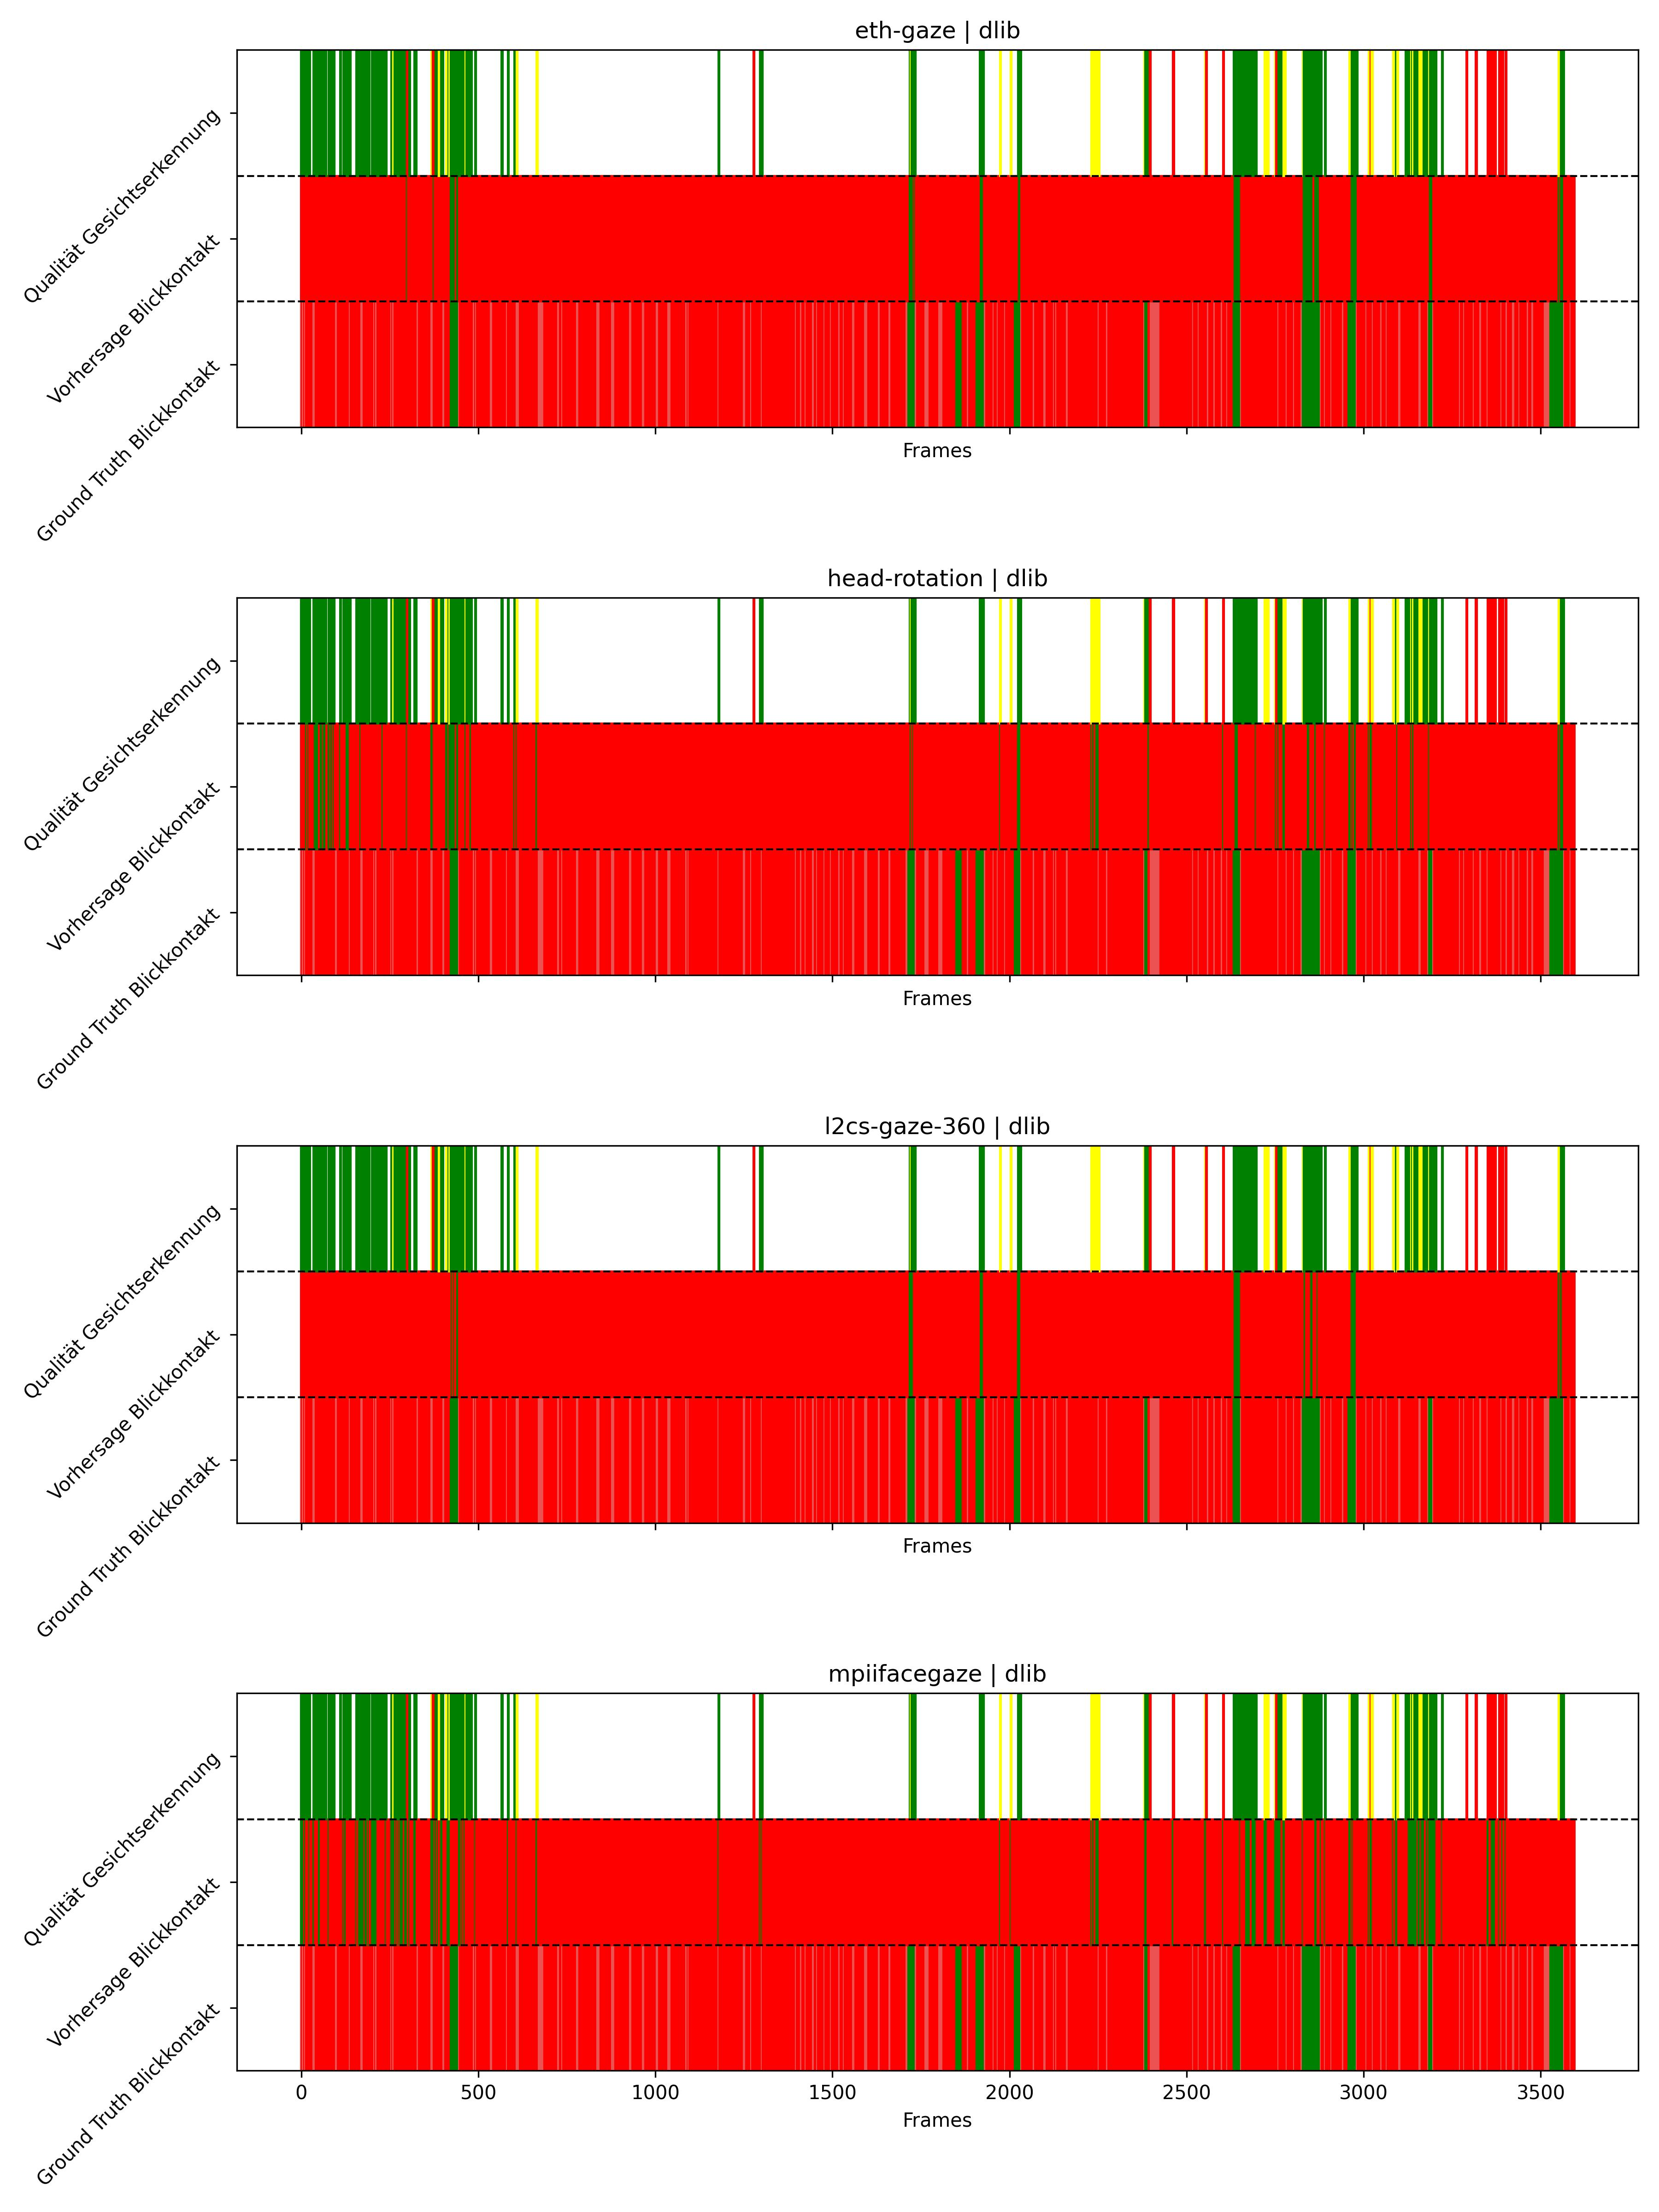
\includegraphics[width=1\linewidth]{appendix/08-dlib-overview-gaze.jpg}
\caption{Überblick über die Ground Truth des Blickkontakts, die Vorhersage des Blickkontakts und die Qualität der Gesichtserkennung mit \dlib. Die Bedeutung der Farben ist in Abbildung \ref{fig:evaluation:gaze:mpiifacegaze} erklärt.  }
\end{figure}

\begin{figure}[H]
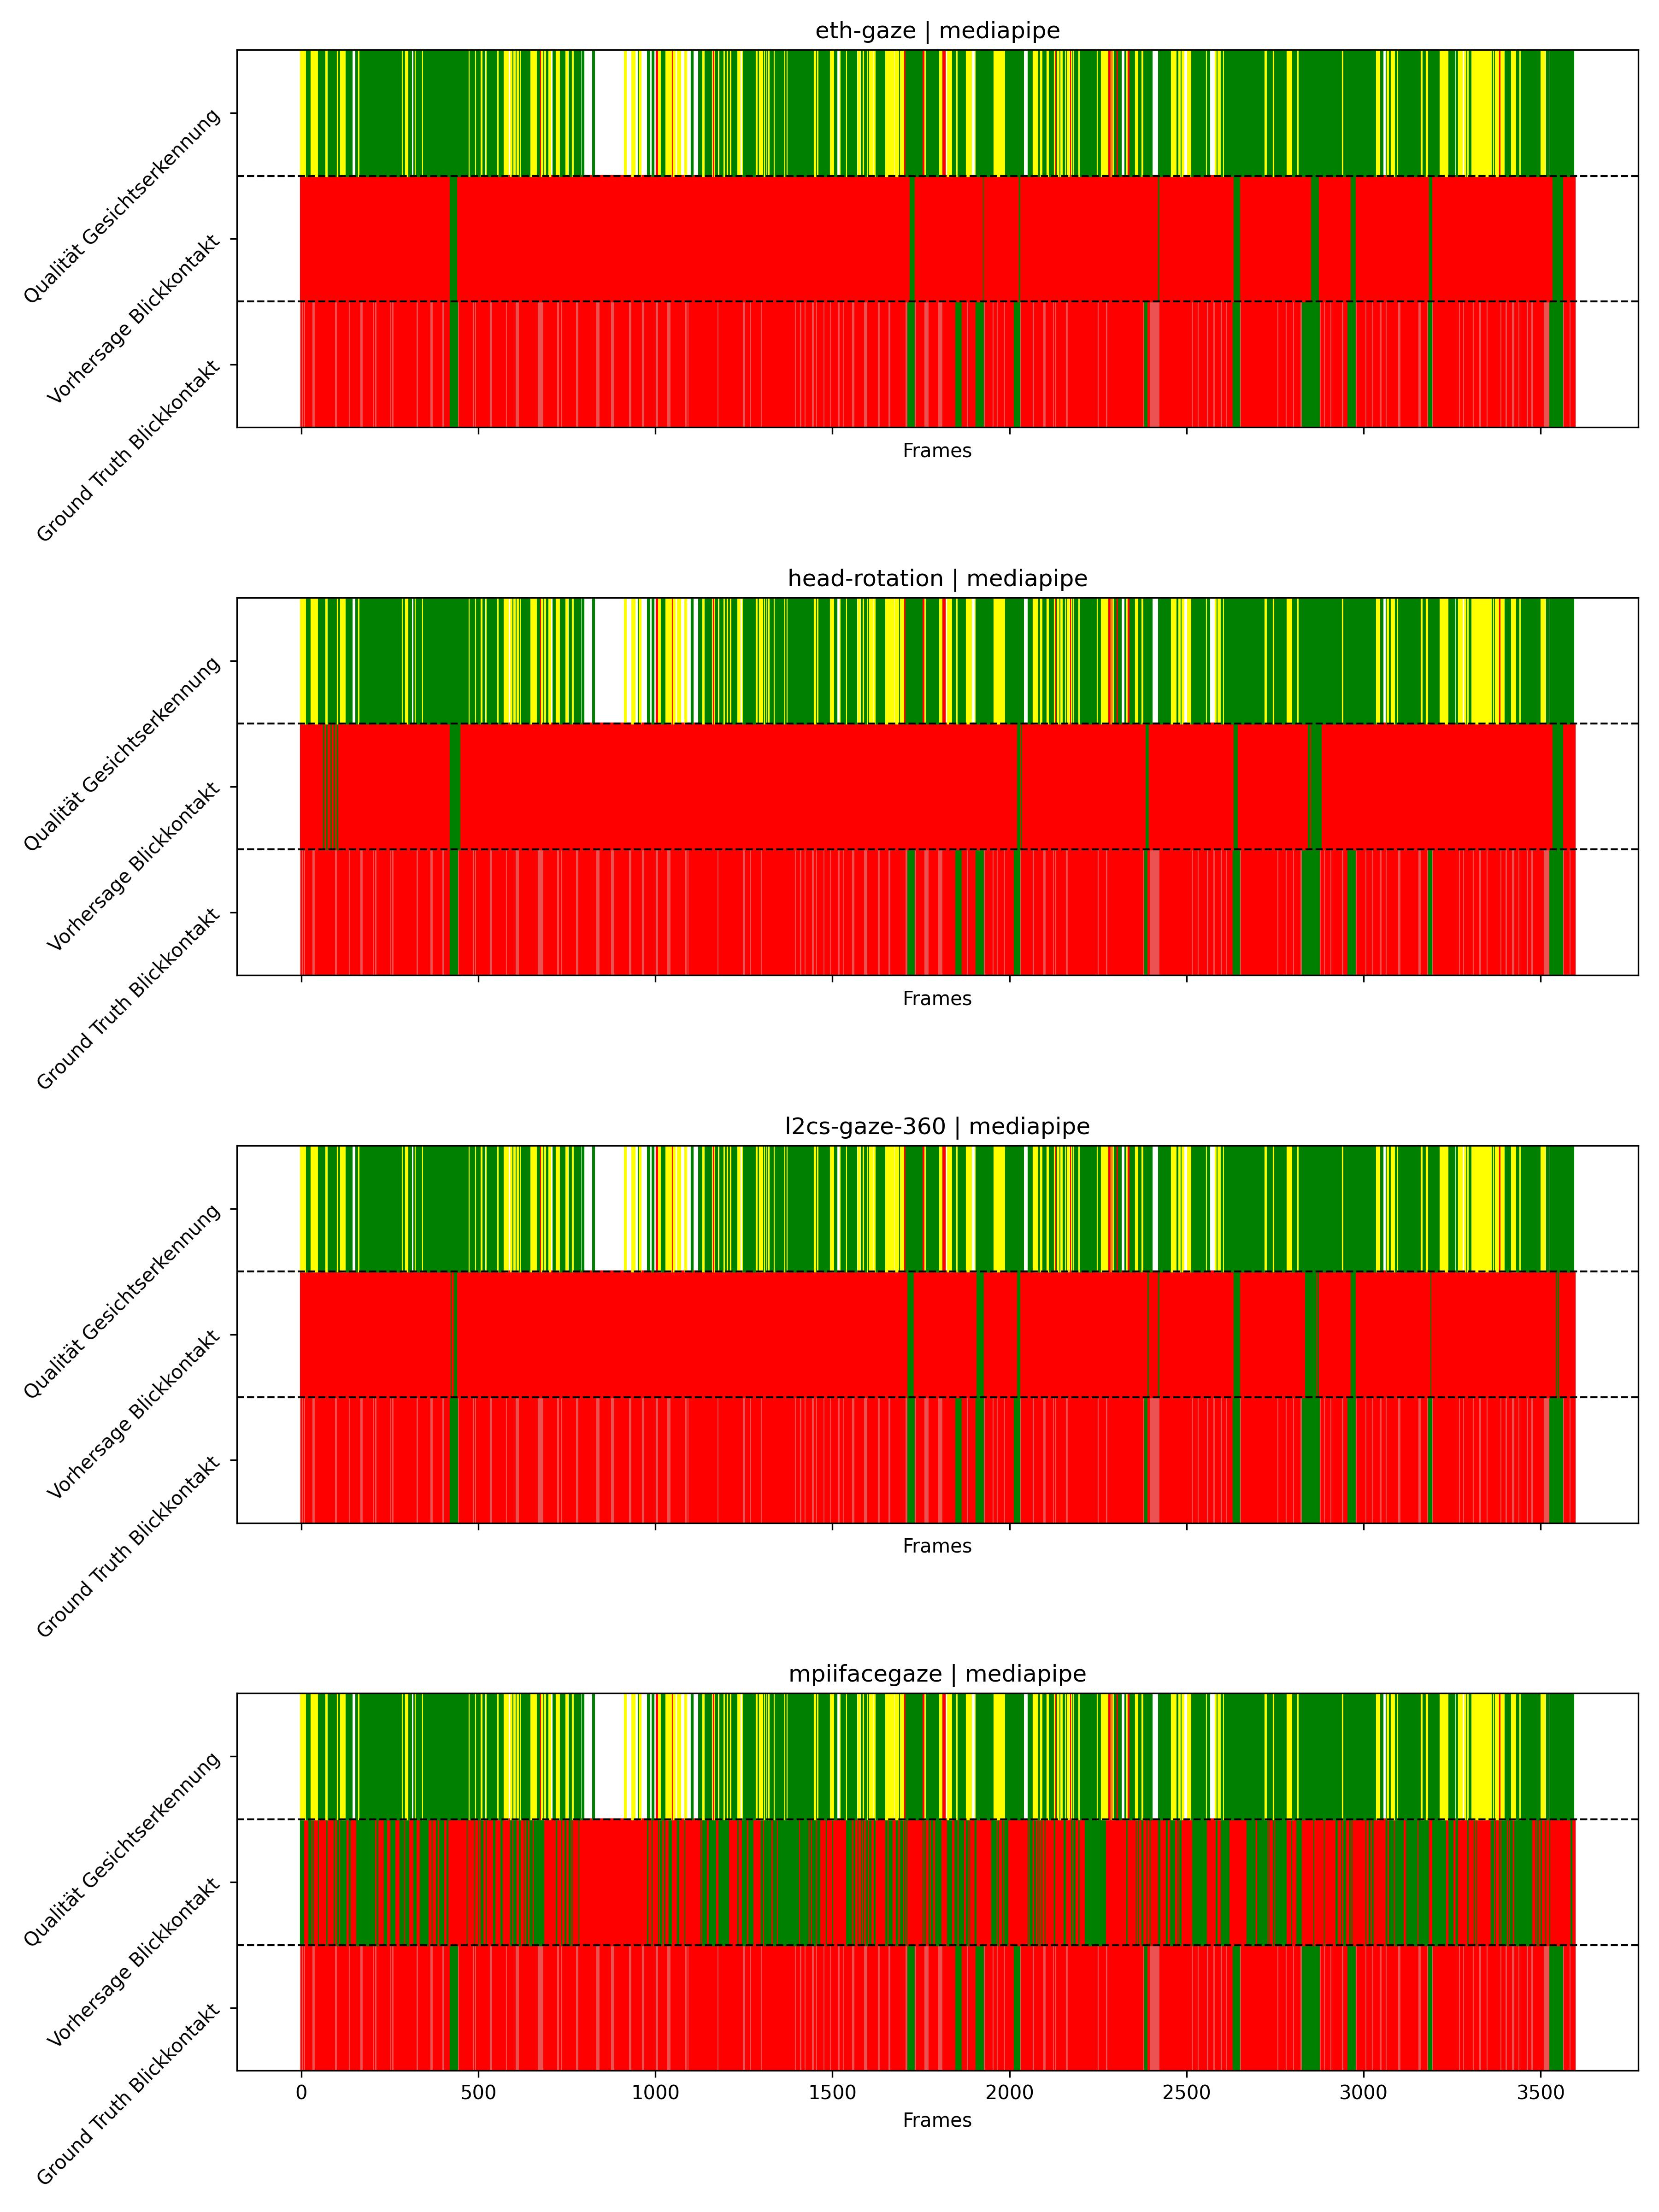
\includegraphics[width=1\linewidth]{appendix/08-mediapipe-overview-gaze.jpg}
\caption{Überblick über die Ground Truth des Blickkontakts, die Vorhersage des Blickkontakts und die Qualität der Gesichtserkennung mit \mediapipe. Die Bedeutung der Farben ist in Abbildung \ref{fig:evaluation:gaze:mpiifacegaze} erklärt.}
\end{figure}

\section{Video 09}\label{appendix:09}
\begin{figure}[H]
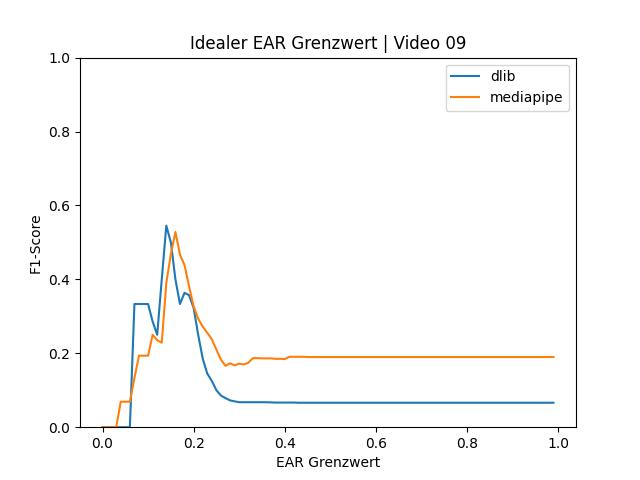
\includegraphics[width=0.7\linewidth]{appendix/09_f1-score-blink.jpg}
\caption{Ergebnisse der Bestimmung des idealen EAR-Grenzwerts für Video 09.}
\end{figure}

\begin{figure}[H]
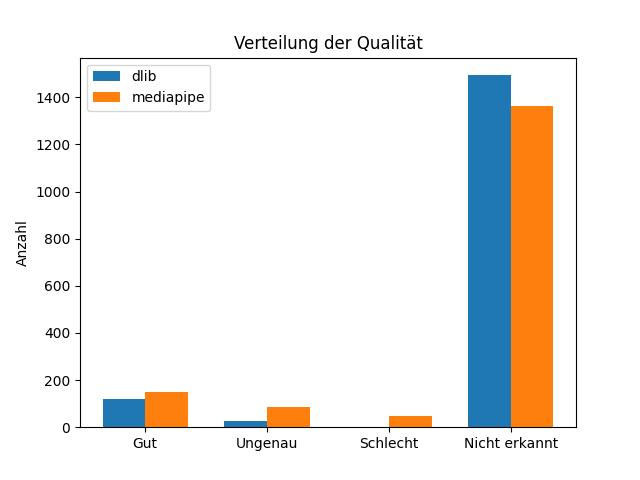
\includegraphics[width=0.7\linewidth]{appendix/09_bar-quality.jpg}
\caption{Aufteilung der Gesichtserkennungsqualität von Video 09.}
\end{figure}

\begin{table}[H]
\centering
\begin{tabular}{l|l|c c |c}
\toprule
\textbf{Gesichtserkennung} & \textbf{Blickrichtung} & \textbf{Seitenlänge} $\hitthresholdsize$ & \textbf{Verschiebung} $\hitthresholdposition$ & \textbf{F1-Score} \\ 
\midrule
\multirow{4}*{dlib}& ETH-XGaze & 0,163 & 0,047 & 0,949  \\ 
& Gaze360 & 0,214 & 0,084 & 0,949 \\ 
& MPIIFaceGaze & 0,051 & -0,039 & 0,939  \\ 
& Kopfrotation & 0,133 & 0,194 & 0,89  \\ 
\hline\multirow{4}*{MediaPipe}& ETH-XGaze & 0,143 & 0,022 & 0,882  \\ 
& Gaze360 & 0,459 & 0,047 & 0,963 \\ 
& MPIIFaceGaze & 0,051 & -0,027 & 0,724  \\ 
& Kopfrotation & 0,143 & 0,194 & 0,907  \\ 
\bottomrule\end{tabular}
\caption{Ergebnis des Hyperparameter-Tunings für die Zone speziell für Video 09.}
\label{tab:appendix:09:local}
\end{table}
\begin{table}[H]
\centering
\begin{tabular}{l|l|c c c c|c c|c}
\toprule
\textbf{Gesichtserkennung} & \textbf{Blickrichtung} & $TP$ & $TN$& $FP$ & $FN$ & \textbf{Precision} & \textbf{Recall} & \textbf{F1-Score} \\ 
\midrule
\multirow{4}*{dlib}& ETH-XGaze & 105 & 1514 & 7 & 14 & 0,938 & 0,882 & 0,909 \\ 
& Gaze360 & 113 & 1513 & 8 & 6 & 0,934 & 0,95 & 0,942 \\ 
& MPIIFaceGaze & 114 & 1503 & 18 & 5 & 0,864 & 0,958 & 0,908 \\ 
& Kopfrotation & 110 & 1499 & 22 & 9 & 0,833 & 0,924 & 0,876 \\ 
\hline\multirow{4}*{MediaPipe}& ETH-XGaze & 107 & 1490 & 32 & 12 & 0,77 & 0,899 & 0,829 \\ 
& Gaze360 & 116 & 1514 & 8 & 3 & 0,935 & 0,975 & 0,955 \\ 
& MPIIFaceGaze & 105 & 1456 & 66 & 14 & 0,614 & 0,882 & 0,724 \\ 
& Kopfrotation & 107 & 1505 & 17 & 12 & 0,863 & 0,899 & 0,881 \\ 
\bottomrule\end{tabular}
\caption{Zusammensetzung des F1-Scores unter Verwendung der in Kapitel \ref{sec:evaluation:results:gaze:threshold} bestimmten globalen Parameter $\hitthresholdsize$ und $\hitthresholdposition$.}
\label{tab:appendix:09:f1}
\end{table}
\begin{figure}[H]
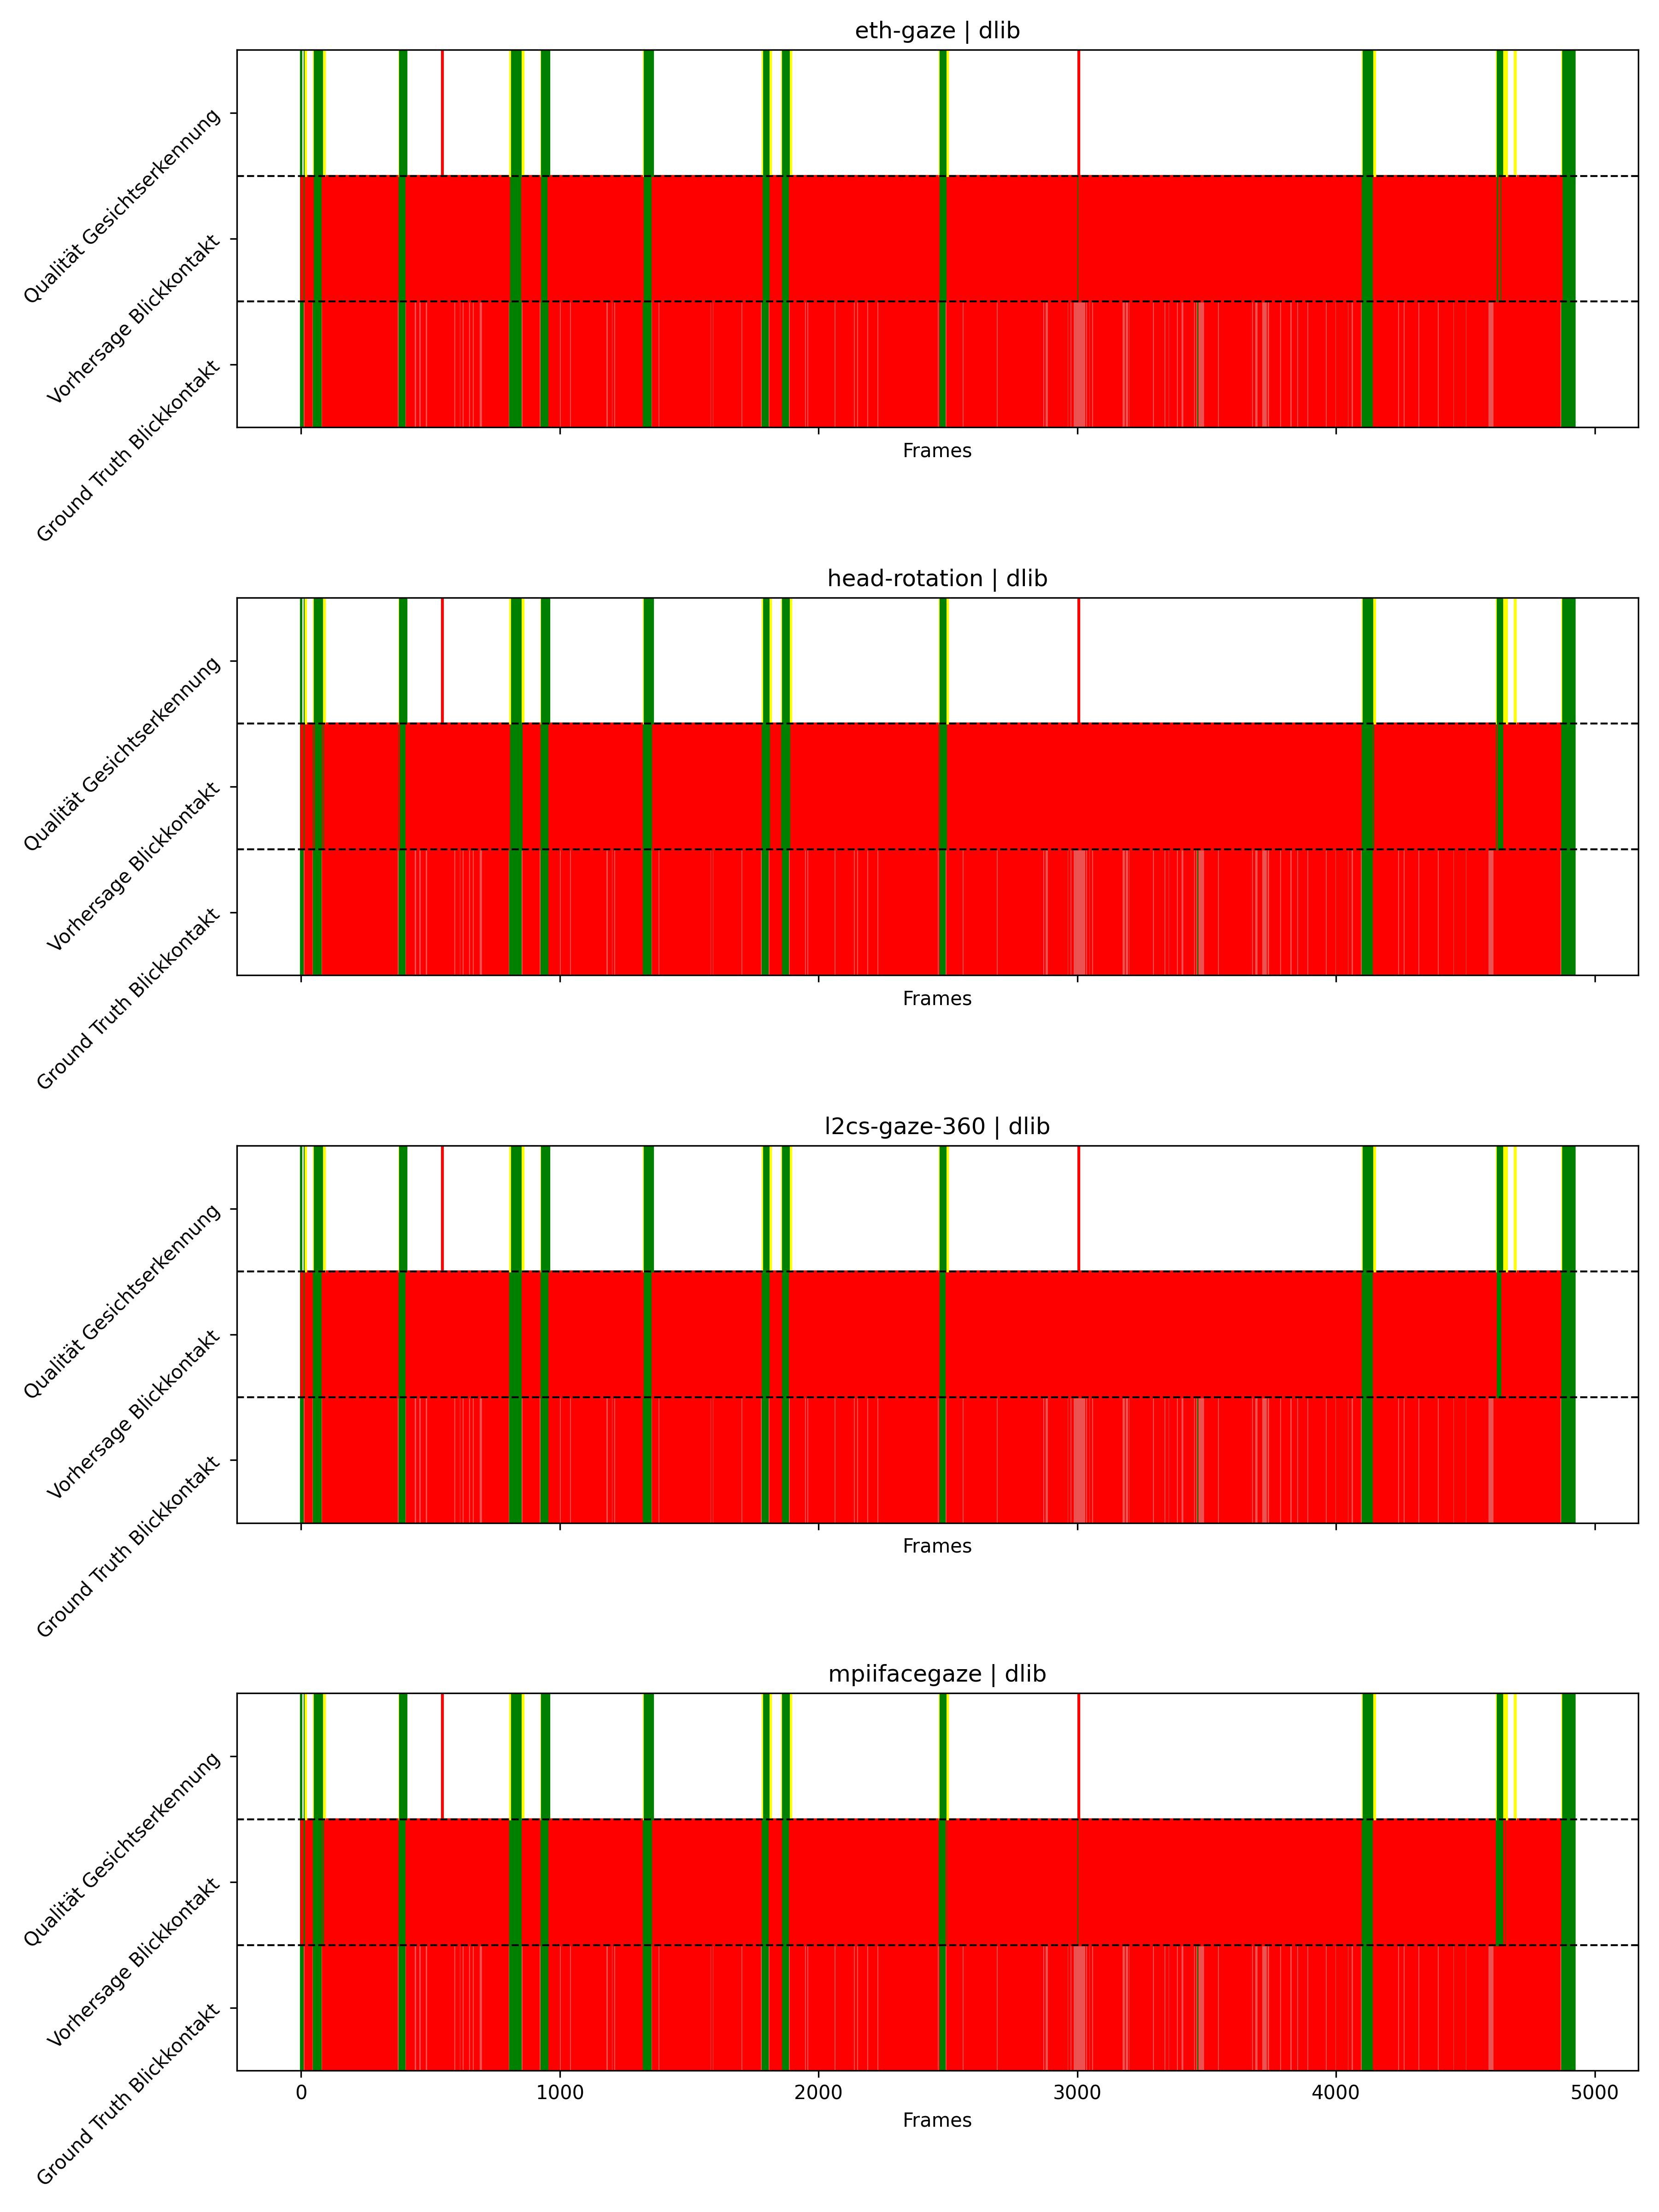
\includegraphics[width=1\linewidth]{appendix/09-dlib-overview-gaze.jpg}
\caption{Überblick über die Ground Truth des Blickkontakts, die Vorhersage des Blickkontakts und die Qualität der Gesichtserkennung mit \dlib. Die Bedeutung der Farben ist in Abbildung \ref{fig:evaluation:gaze:mpiifacegaze} erklärt.   }
\label{fig:appendix:09:dlib}
\end{figure}

\begin{figure}[H]
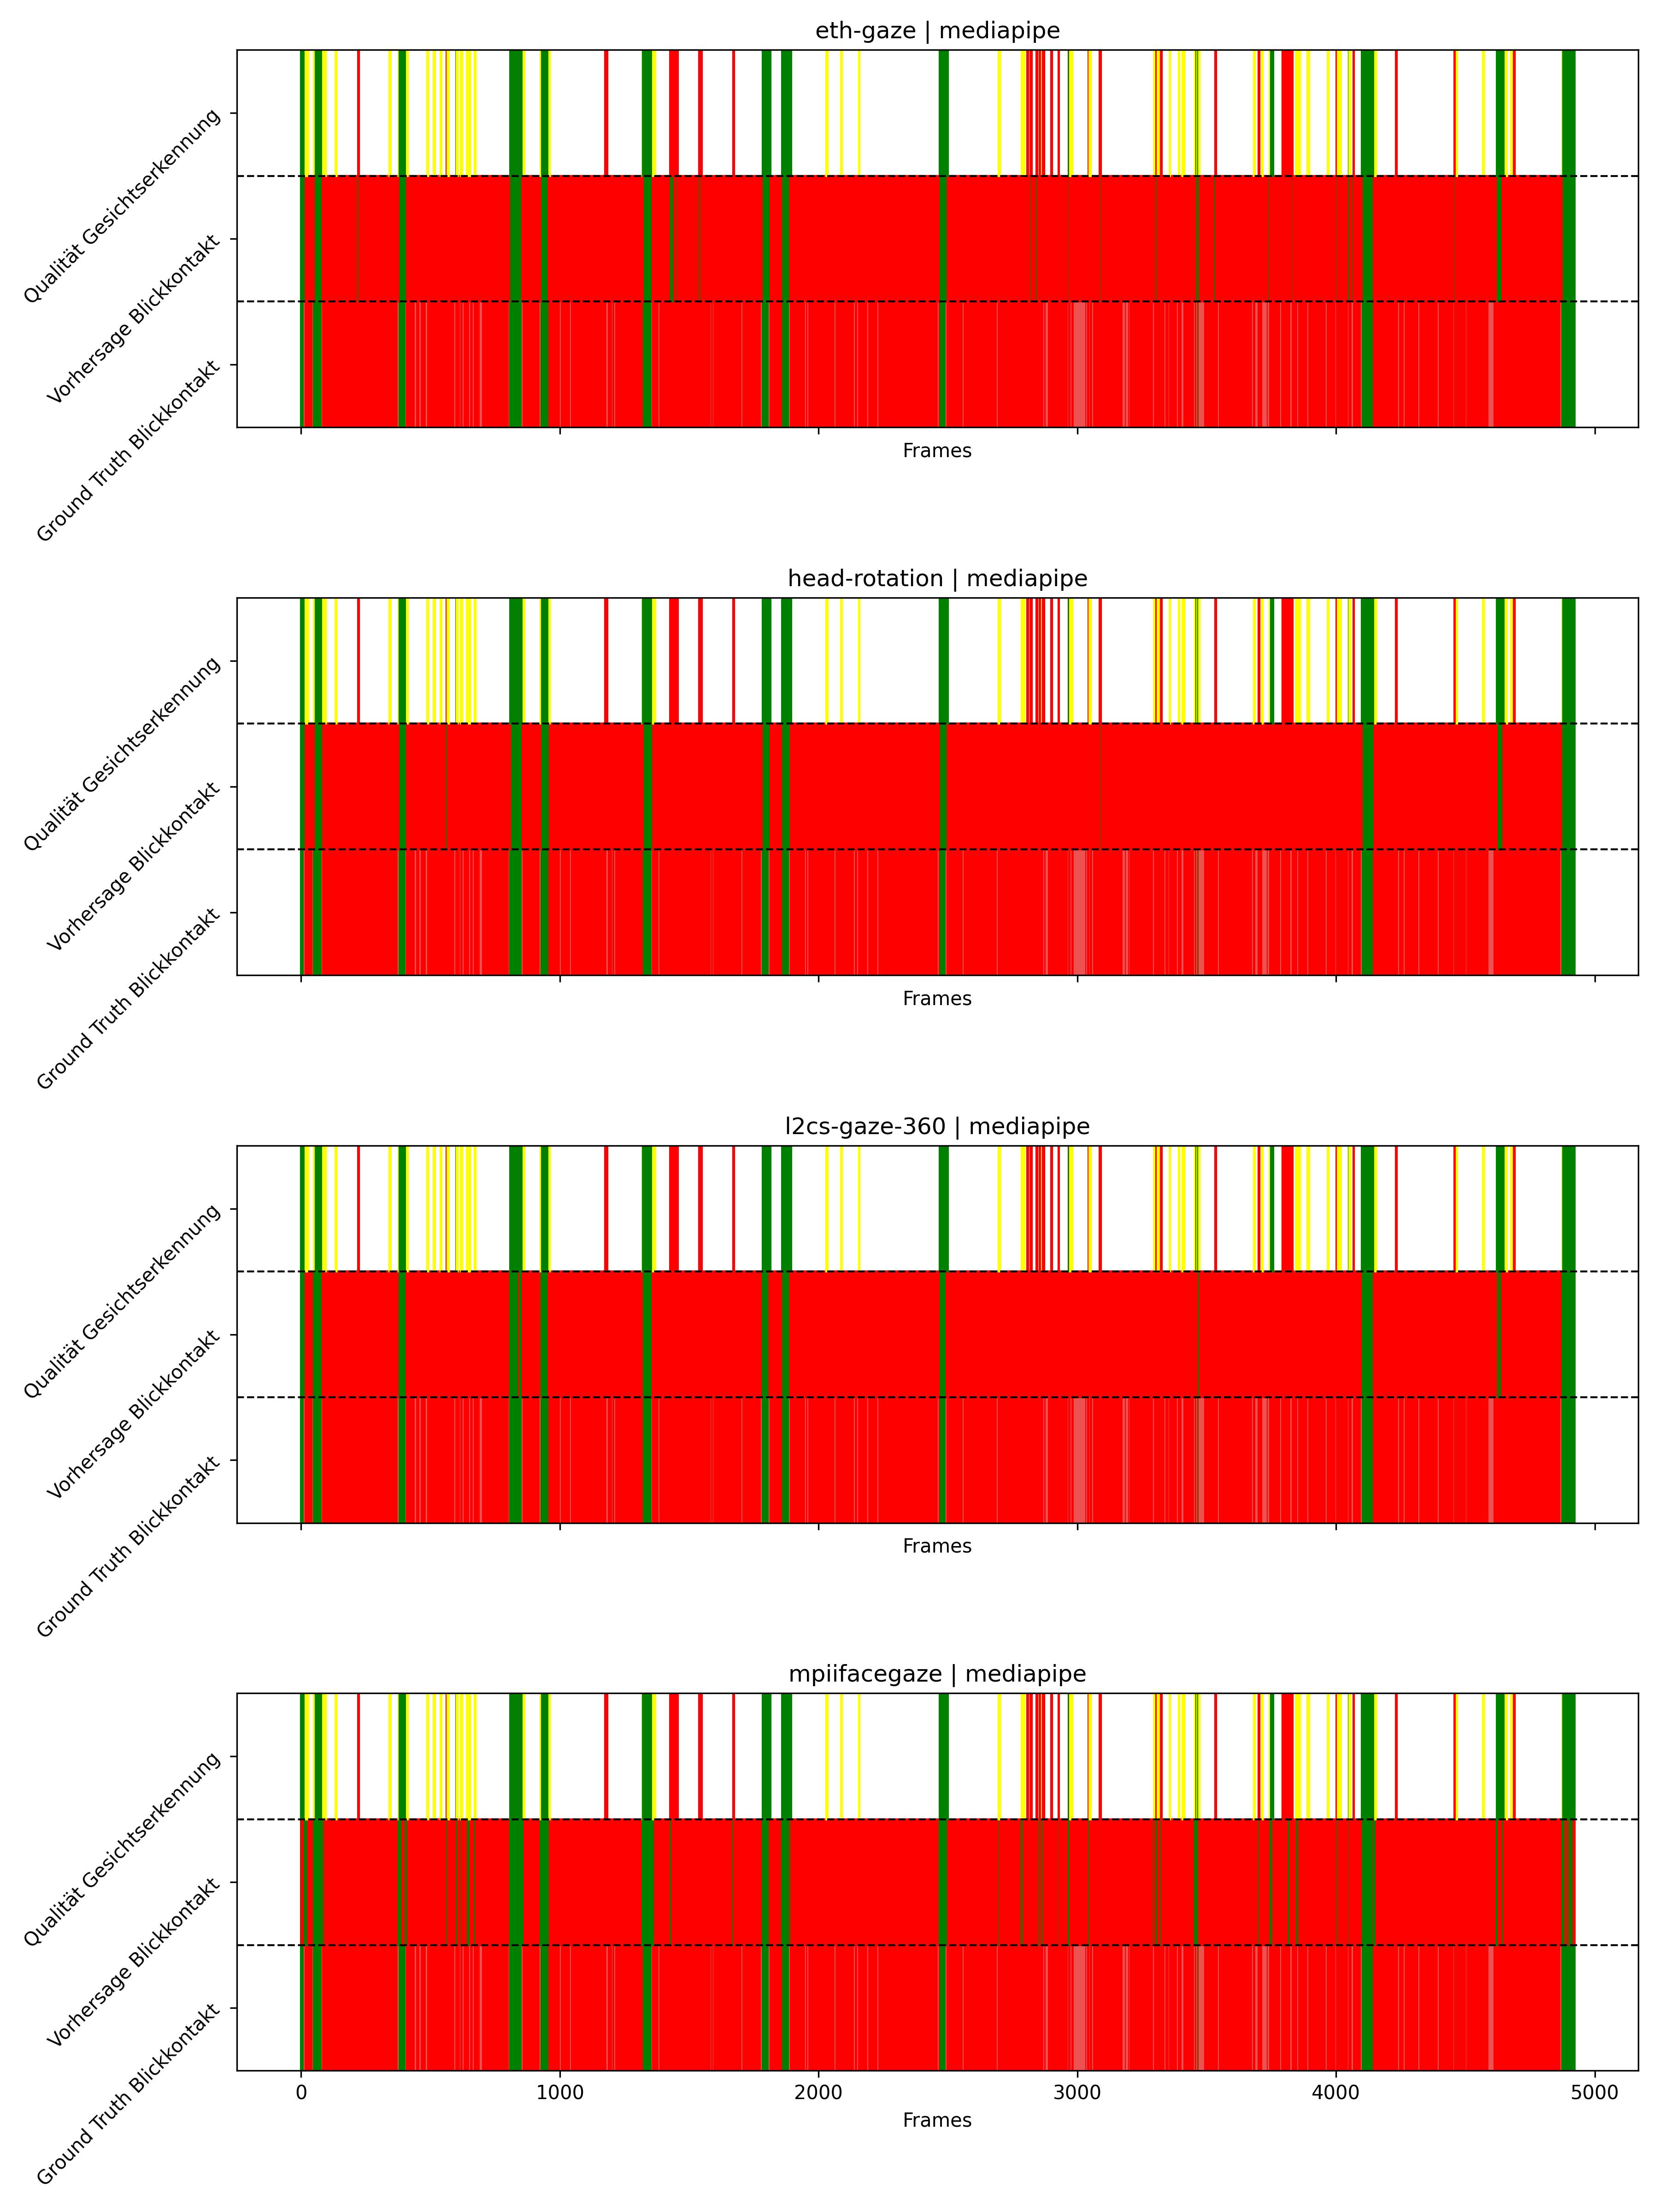
\includegraphics[width=1\linewidth]{appendix/09-mediapipe-overview-gaze.jpg}
\caption{Überblick über die Ground Truth des Blickkontakts, die Vorhersage des Blickkontakts und die Qualität der Gesichtserkennung mit \mediapipe. Die Bedeutung der Farben ist in Abbildung \ref{fig:evaluation:gaze:mpiifacegaze} erklärt.}
\label{fig:appendix:09:mediapipe}
\end{figure}

\section{Video 10}
\begin{figure}[H]
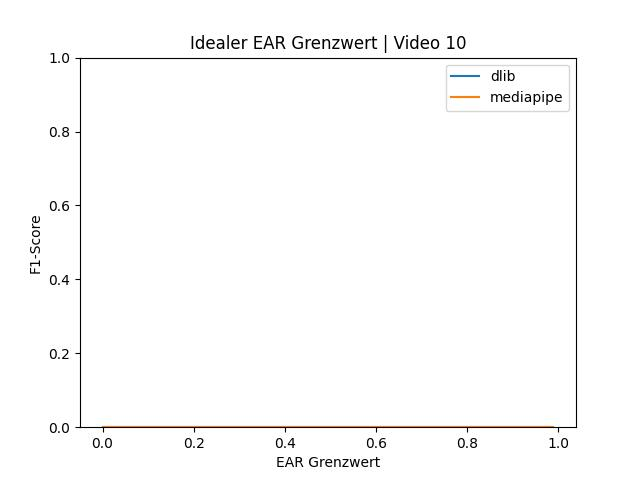
\includegraphics[width=0.7\linewidth]{appendix/10_f1-score-blink.jpg}
\caption{Ergebnisse der Bestimmung des idealen EAR-Grenzwerts für Video 10. Durch die Sonnenbrille von \philipp waren die Augen in keinem der Bilder zu sehen.}
\end{figure}

\begin{figure}[H]
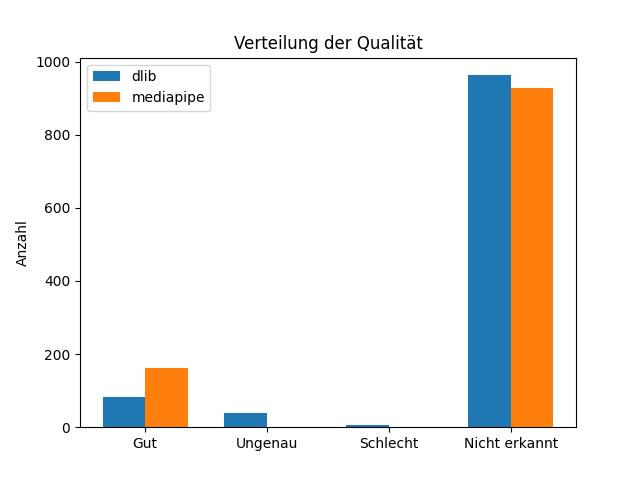
\includegraphics[width=0.7\linewidth]{appendix/10_bar-quality.jpg}
\caption{Aufteilung der Gesichtserkennungsqualität von Video 10.}
\end{figure}

\begin{table}[H]
\centering
\begin{tabular}{l|l|c c |c}
\toprule
\textbf{Gesichtserkennung} & \textbf{Blickrichtung} & \textbf{Seitenlänge} $\hitthresholdsize$ & \textbf{Verschiebung} $\hitthresholdposition$ & \textbf{F1-Score} \\ 
\midrule
\multirow{4}*{dlib}& ETH-XGaze & 0,276 & 0,133 & 0,891  \\ 
& Gaze360 & 0,49 & 0,145 & 0,63 \\ 
& MPIIFaceGaze & 0,092 & 0,022 & 0,891  \\ 
& Kopfrotation & 0,265 & 0,218 & 0,891  \\ 
\hline\multirow{4}*{MediaPipe}& ETH-XGaze & 0,245 & 0,133 & 0,963  \\ 
& Gaze360 & 0,5 & 0,133 & 0,667 \\ 
& MPIIFaceGaze & 0,092 & 0,022 & 0,952  \\ 
& Kopfrotation & 0,214 & 0,255 & 0,977  \\ 
\bottomrule\end{tabular}
\caption{Ergebnis des Hyperparameter-Tunings für die Zone speziell für Video 10.}
\label{tab:appendix:10:local}
\end{table}
\begin{table}[H]
\centering
\begin{tabular}{l|l|c c c c|c c|c}
\toprule
\textbf{Gesichtserkennung} & \textbf{Blickrichtung} & $TP$ & $TN$& $FP$ & $FN$ & \textbf{Precision} & \textbf{Recall} & \textbf{F1-Score} \\ 
\midrule
\multirow{4}*{dlib}& ETH-XGaze & 71 & 941 & 1 & 77 & 0,986 & 0,48 & 0,645 \\ 
& Gaze360 & 47 & 942 & 0 & 101 & 1,0 & 0,318 & 0,482 \\ 
& MPIIFaceGaze & 40 & 942 & 0 & 108 & 1,0 & 0,27 & 0,426 \\ 
& Kopfrotation & 121 & 938 & 4 & 27 & 0,968 & 0,818 & 0,886 \\ 
\hline\multirow{4}*{MediaPipe}& ETH-XGaze & 64 & 942 & 0 & 84 & 1,0 & 0,432 & 0,604 \\ 
& Gaze360 & 45 & 942 & 0 & 103 & 1,0 & 0,304 & 0,466 \\ 
& MPIIFaceGaze & 52 & 931 & 11 & 96 & 0,825 & 0,351 & 0,493 \\ 
& Kopfrotation & 130 & 942 & 0 & 18 & 1,0 & 0,878 & 0,935 \\ 
\bottomrule\end{tabular}
\caption{Zusammensetzung des F1-Scores unter Verwendung der in Kapitel \ref{sec:evaluation:results:gaze:threshold} bestimmten globalen Parameter $\hitthresholdsize$ und $\hitthresholdposition$.}
\label{tab:appendix:10:f1}
\end{table}

\begin{figure}[H]
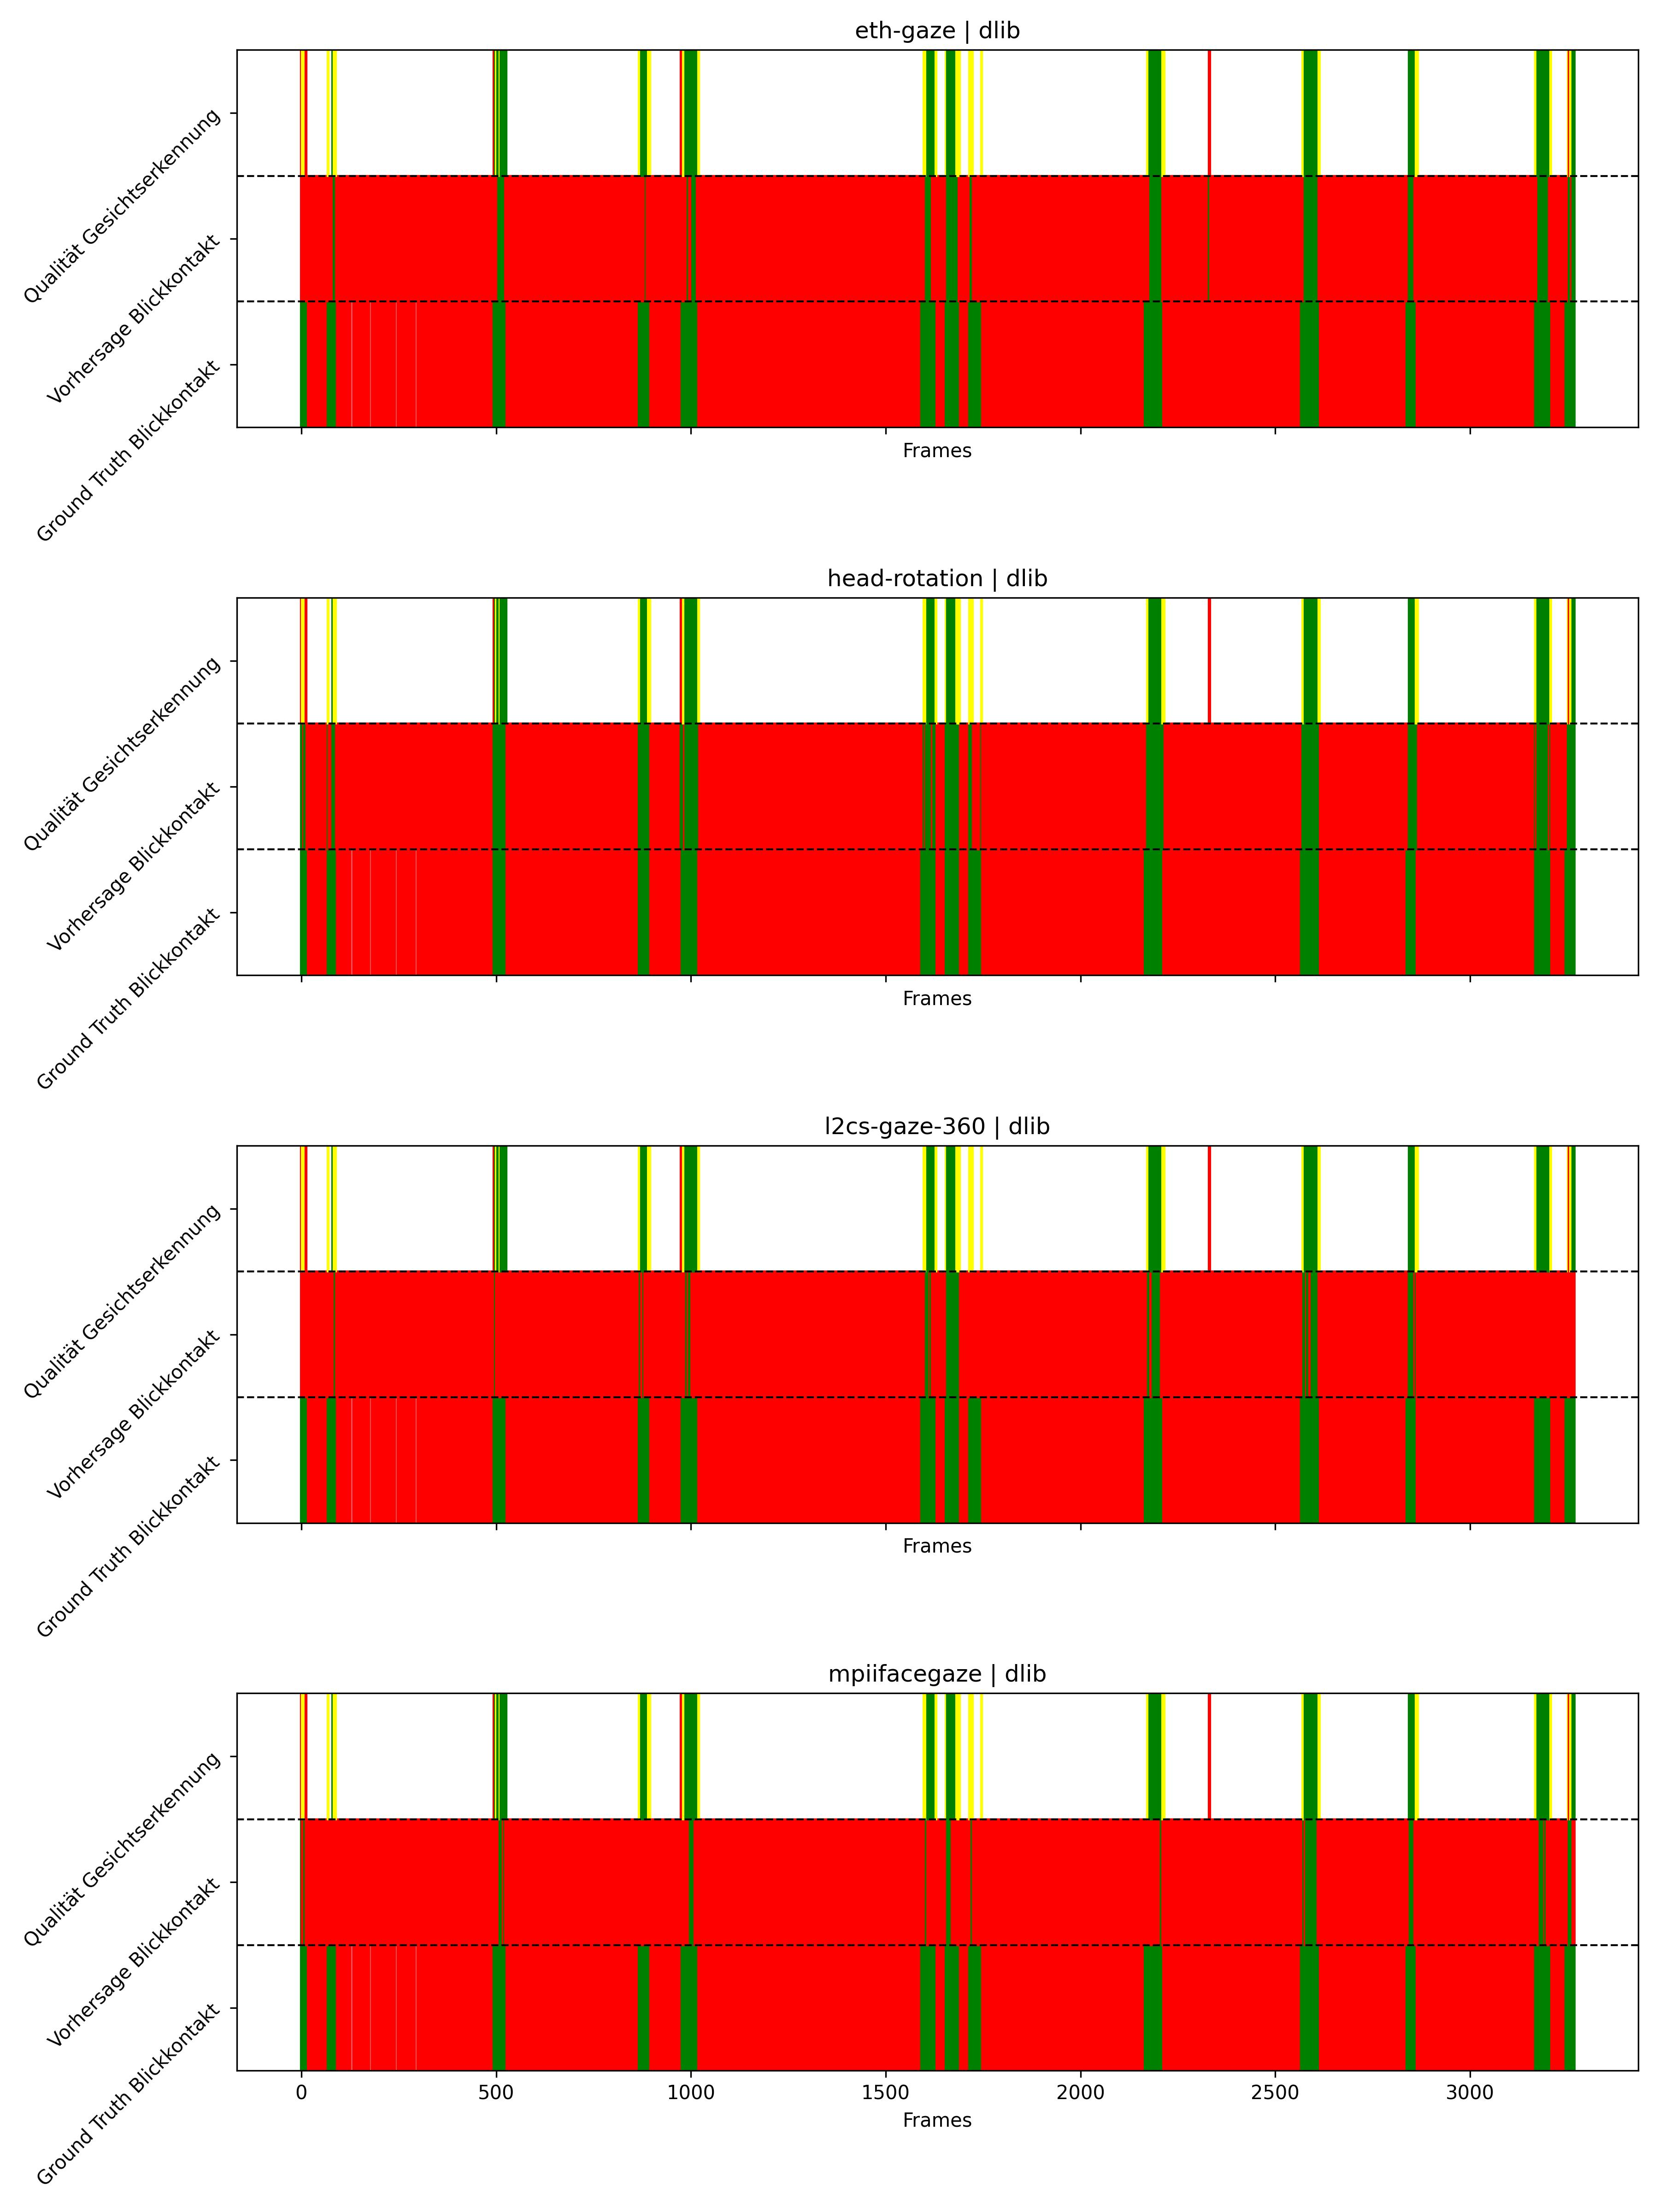
\includegraphics[width=1\linewidth]{appendix/10-dlib-overview-gaze.jpg}
\caption{Überblick über die Ground Truth des Blickkontakts, die Vorhersage des Blickkontakts und die Qualität der Gesichtserkennung mit \dlib. Die Bedeutung der Farben ist in Abbildung \ref{fig:evaluation:gaze:mpiifacegaze} erklärt.   }
\end{figure}

\begin{figure}[H]
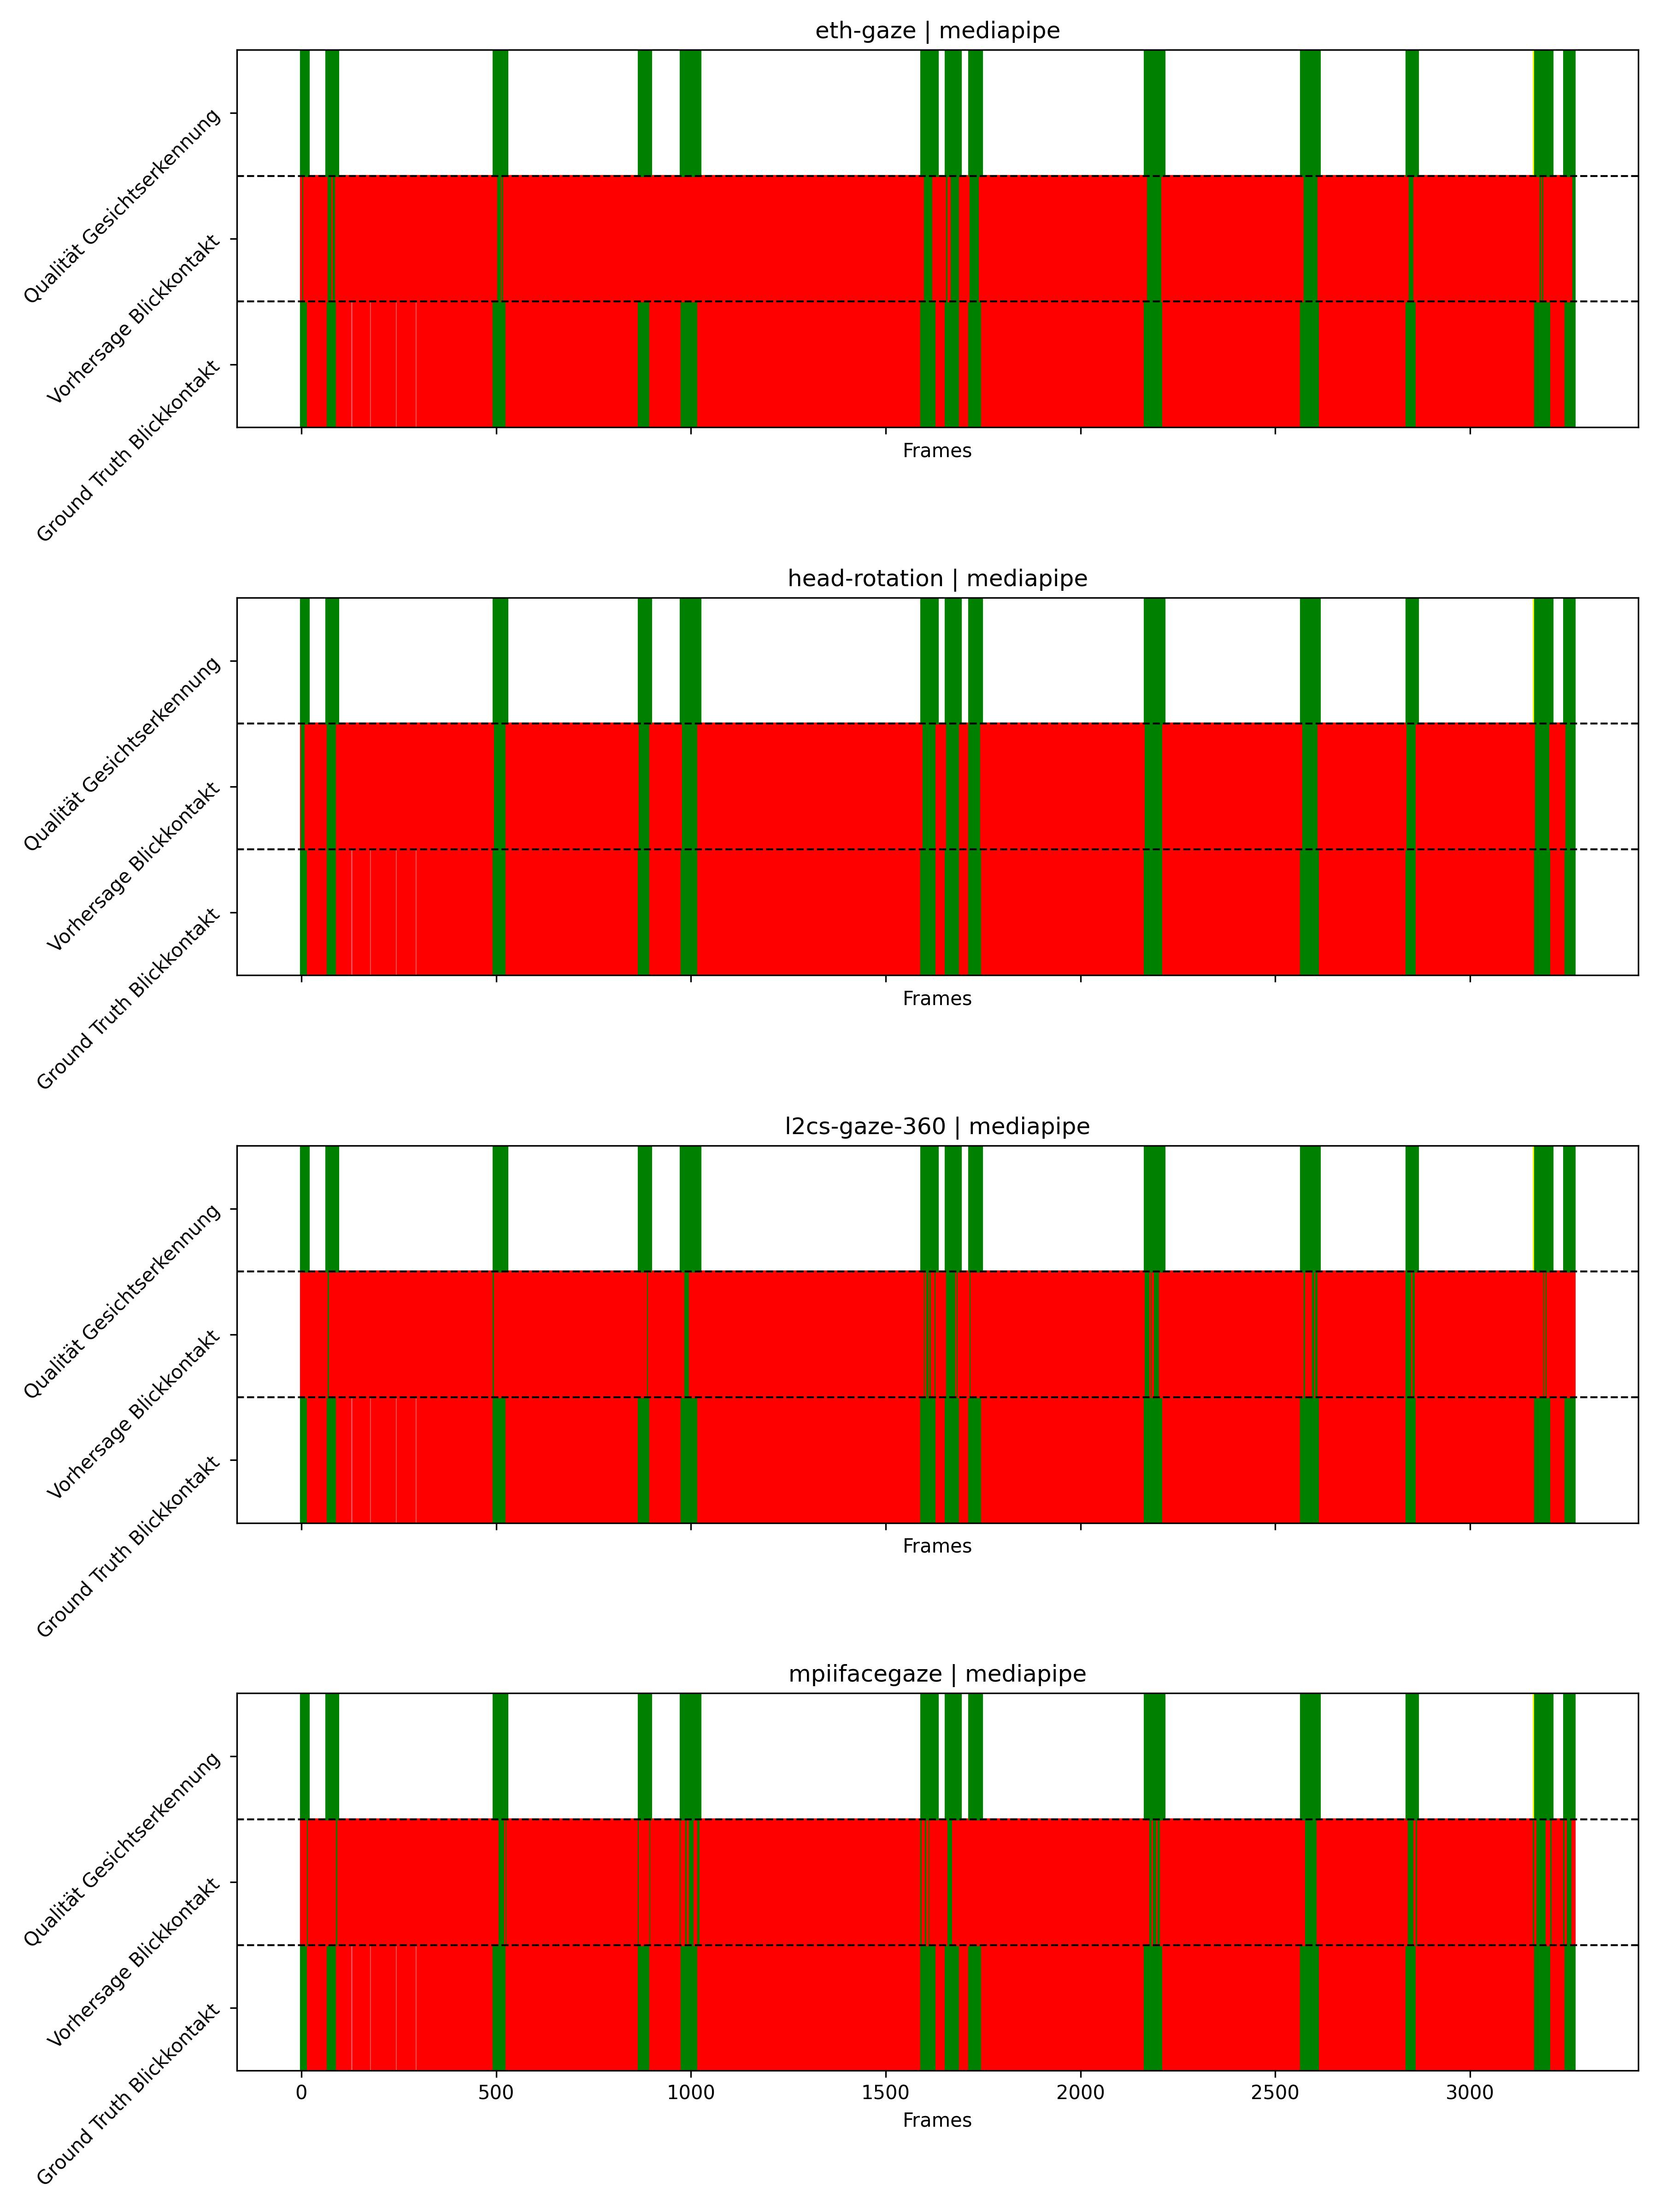
\includegraphics[width=1\linewidth]{appendix/10-mediapipe-overview-gaze.jpg}
\caption{Überblick über die Ground Truth des Blickkontakts, die Vorhersage des Blickkontakts und die Qualität der Gesichtserkennung mit \mediapipe. Die Bedeutung der Farben ist in Abbildung \ref{fig:evaluation:gaze:mpiifacegaze} erklärt.}
\end{figure}

\section{Video 11}
\begin{figure}[H]
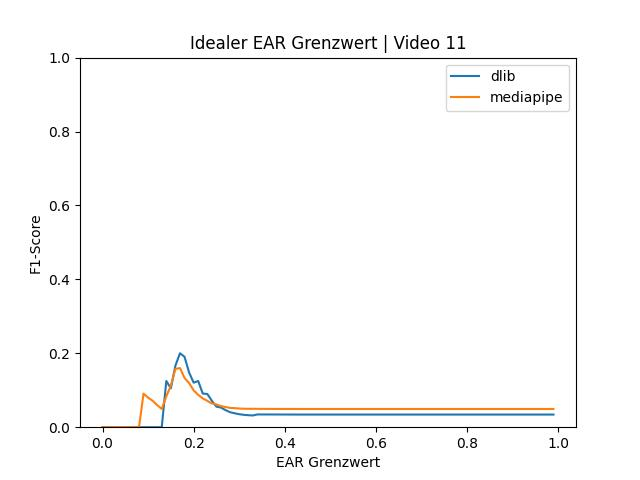
\includegraphics[width=0.7\linewidth]{appendix/11_f1-score-blink.jpg}
\caption{Ergebnisse der Bestimmung des idealen EAR-Grenzwerts für Video 11.}
\end{figure}

\begin{figure}[H]
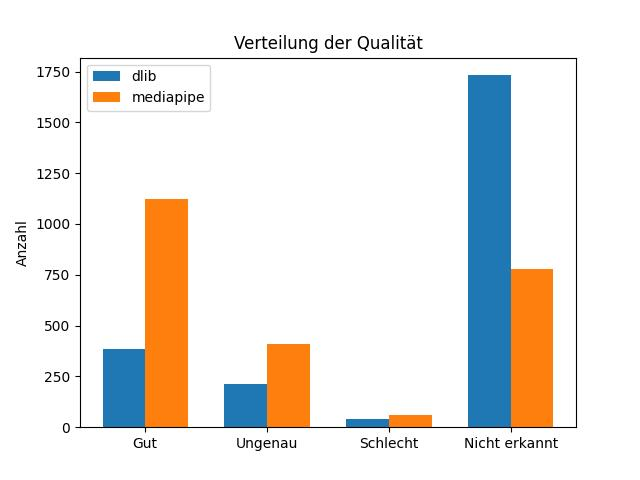
\includegraphics[width=0.7\linewidth]{appendix/11_bar-quality.jpg}
\caption{Aufteilung der Gesichtserkennungsqualität von Video 11.}
\end{figure}

\begin{table}[H]
\centering
\begin{tabular}{l|l|c c |c}
\toprule
\textbf{Gesichtserkennung} & \textbf{Blickrichtung} & \textbf{Seitenlänge} $\hitthresholdsize$ & \textbf{Verschiebung} $\hitthresholdposition$ & \textbf{F1-Score} \\ 
\midrule
\multirow{4}*{dlib}& ETH-XGaze & 0,286 & 0,01 & 0,912  \\ 
& Gaze360 & 0,49 & 0,047 & 0,843 \\ 
& MPIIFaceGaze & 0,112 & -0,002 & 0,721  \\ 
& Kopfrotation & 0,398 & 0,182 & 0,772  \\ 
\hline\multirow{4}*{MediaPipe}& ETH-XGaze & 0,408 & 0,01 & 0,957  \\ 
& Gaze360 & 0,49 & 0,047 & 0,822 \\ 
& MPIIFaceGaze & 0,173 & -0,027 & 0,442  \\ 
& Kopfrotation & 0,5 & 0,218 & 0,865  \\ 
\bottomrule\end{tabular}
\caption{Ergebnis des Hyperparameter-Tunings für die Zone speziell für Video 11.}
\label{tab:appendix:11:local}
\end{table}
\begin{table}[H]
\centering
\begin{tabular}{l|l|c c c c|c c|c}
\toprule
\textbf{Gesichtserkennung} & \textbf{Blickrichtung} & $TP$ & $TN$& $FP$ & $FN$ & \textbf{Precision} & \textbf{Recall} & \textbf{F1-Score} \\ 
\midrule
\multirow{4}*{dlib}& ETH-XGaze & 356 & 1909 & 11 & 85 & 0,97 & 0,807 & 0,881 \\ 
& Gaze360 & 342 & 1892 & 28 & 99 & 0,924 & 0,776 & 0,843 \\ 
& MPIIFaceGaze & 354 & 1726 & 194 & 87 & 0,646 & 0,803 & 0,716 \\ 
& Kopfrotation & 326 & 1785 & 135 & 115 & 0,707 & 0,739 & 0,723 \\ 
\hline\multirow{4}*{MediaPipe}& ETH-XGaze & 404 & 1910 & 15 & 37 & 0,964 & 0,916 & 0,94 \\ 
& Gaze360 & 348 & 1863 & 62 & 93 & 0,849 & 0,789 & 0,818 \\ 
& MPIIFaceGaze & 256 & 1295 & 630 & 185 & 0,289 & 0,58 & 0,386 \\ 
& Kopfrotation & 323 & 1892 & 33 & 118 & 0,907 & 0,732 & 0,811 \\ 
\bottomrule\end{tabular}
\caption{Zusammensetzung des F1-Scores unter Verwendung der in Kapitel \ref{sec:evaluation:results:gaze:threshold} bestimmten globalen Parameter $\hitthresholdsize$ und $\hitthresholdposition$.}
\label{tab:appendix:11:f1}
\end{table}
\begin{figure}[H]
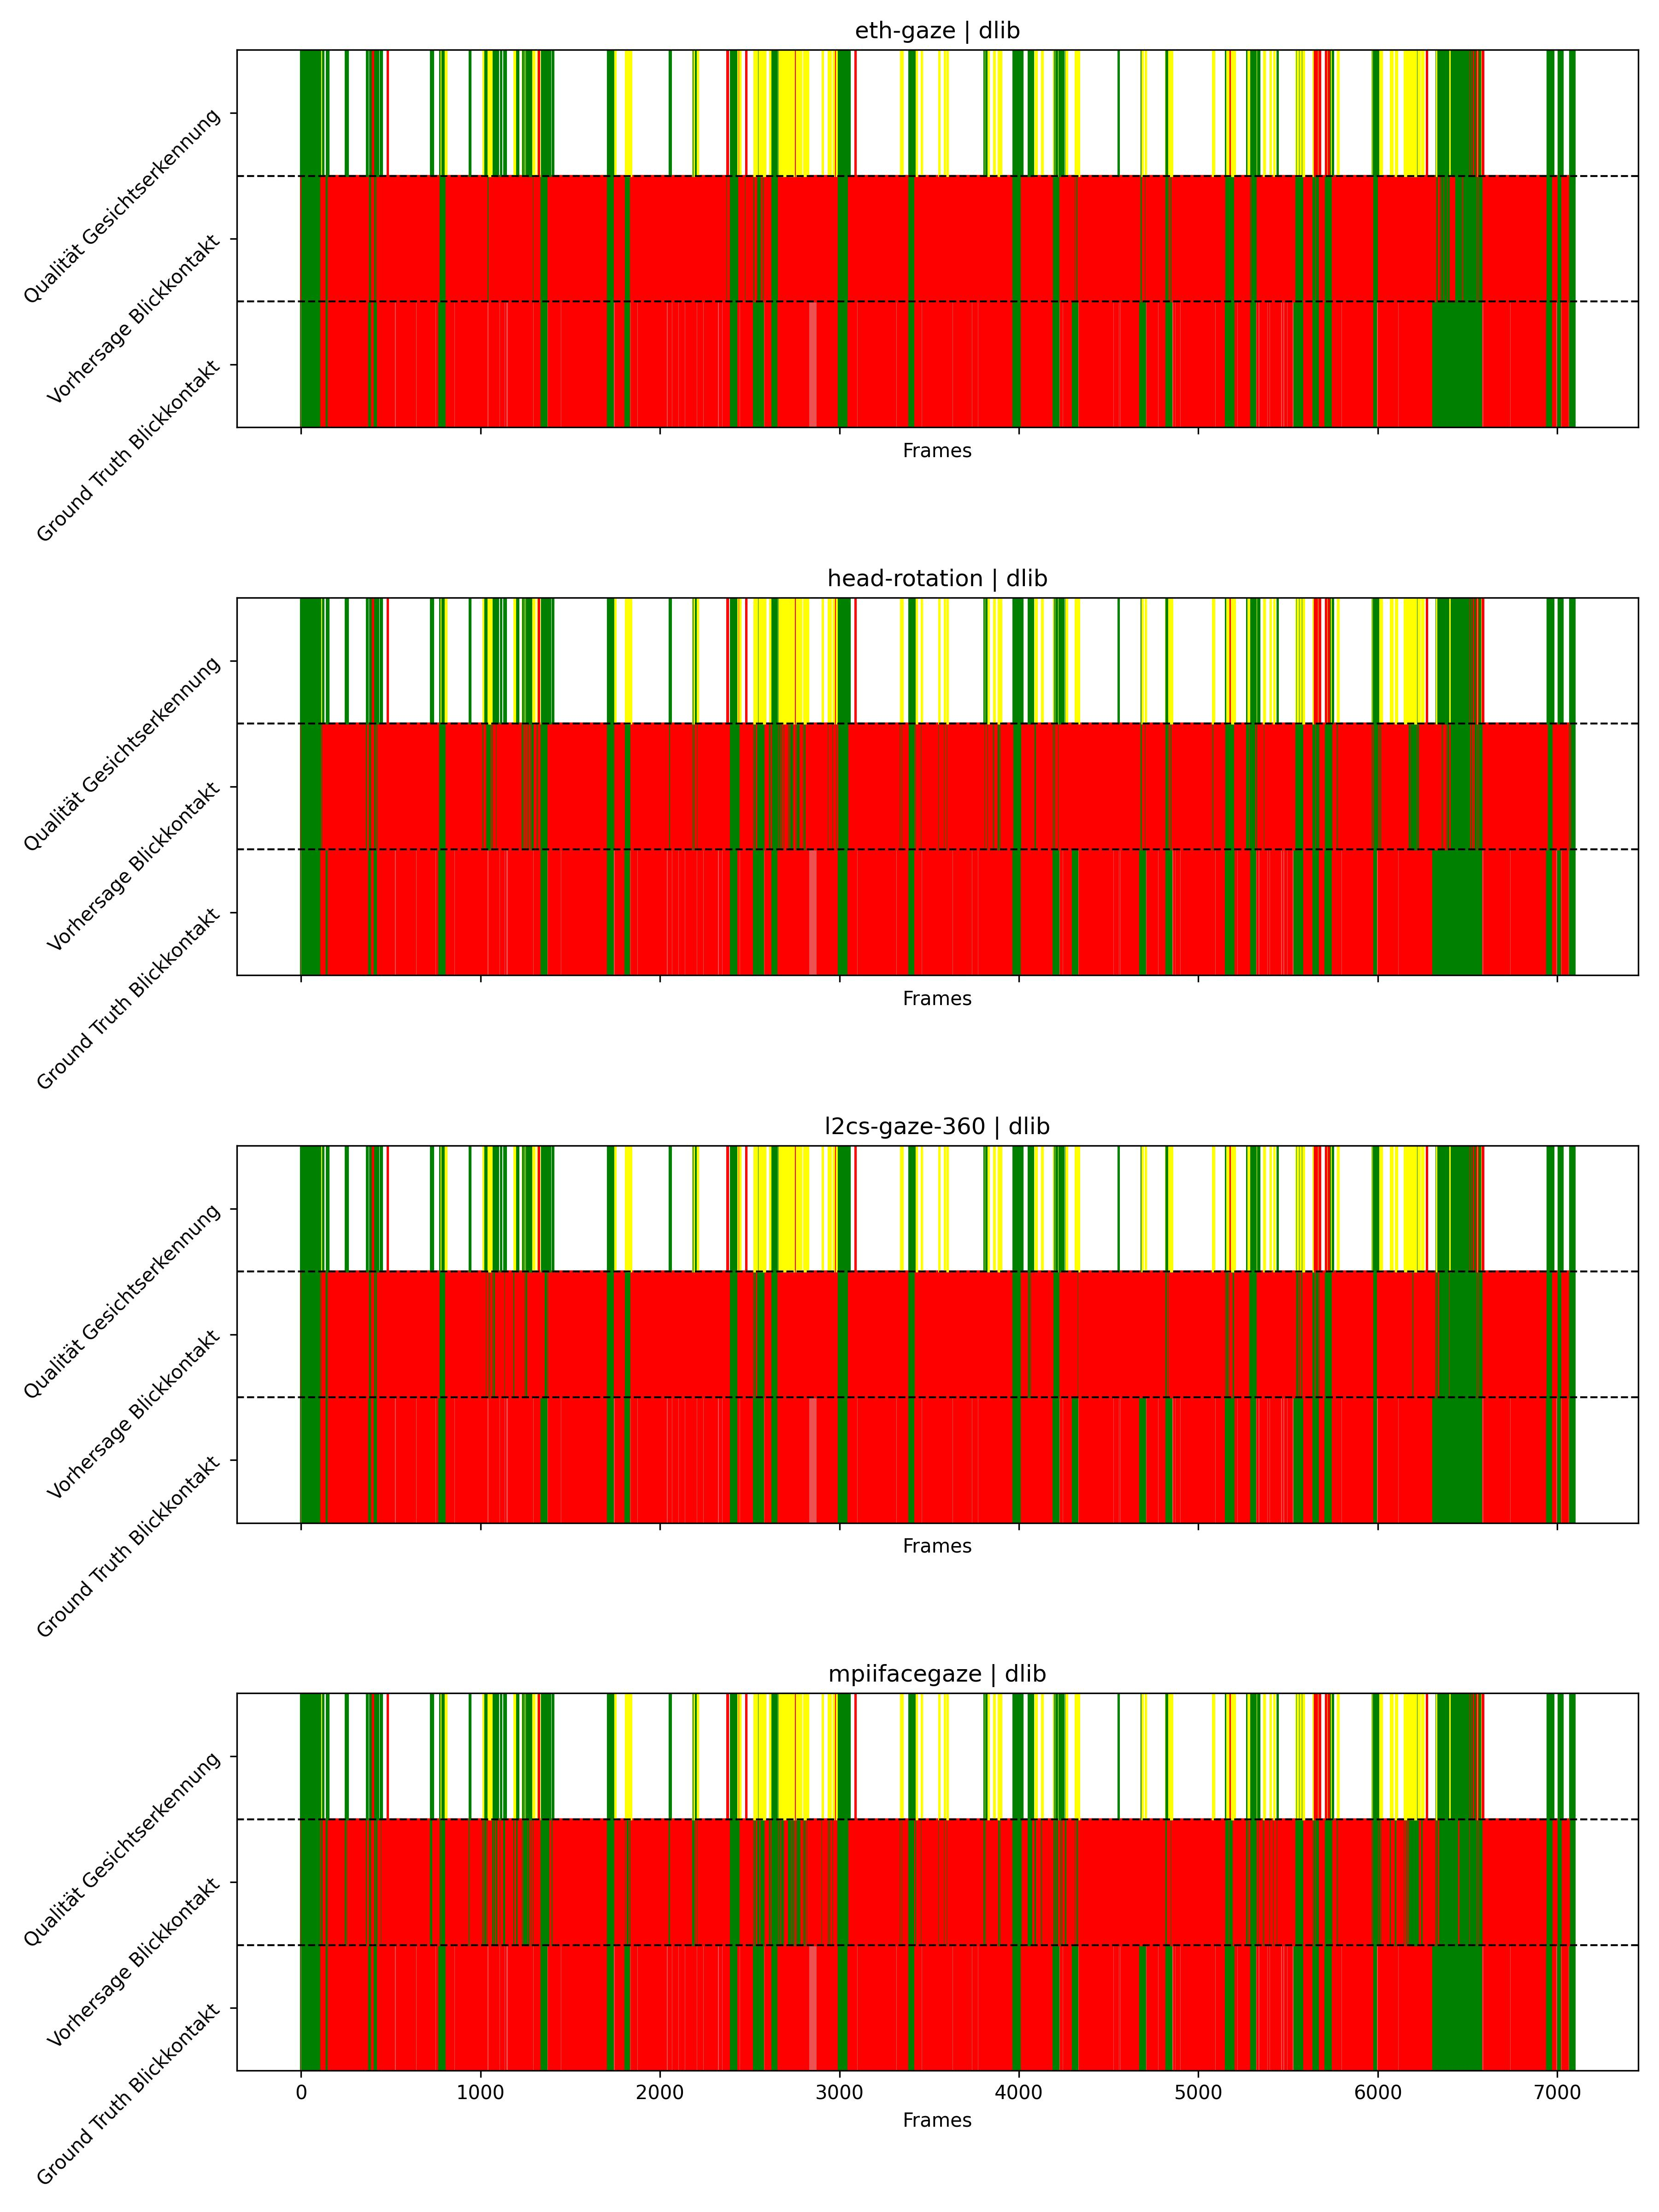
\includegraphics[width=1\linewidth]{appendix/11-dlib-overview-gaze.jpg}
\caption{Überblick über die Ground Truth des Blickkontakts, die Vorhersage des Blickkontakts und die Qualität der Gesichtserkennung mit \dlib. Die Bedeutung der Farben ist in Abbildung \ref{fig:evaluation:gaze:mpiifacegaze} erklärt.  }
\end{figure}

\begin{figure}[H]
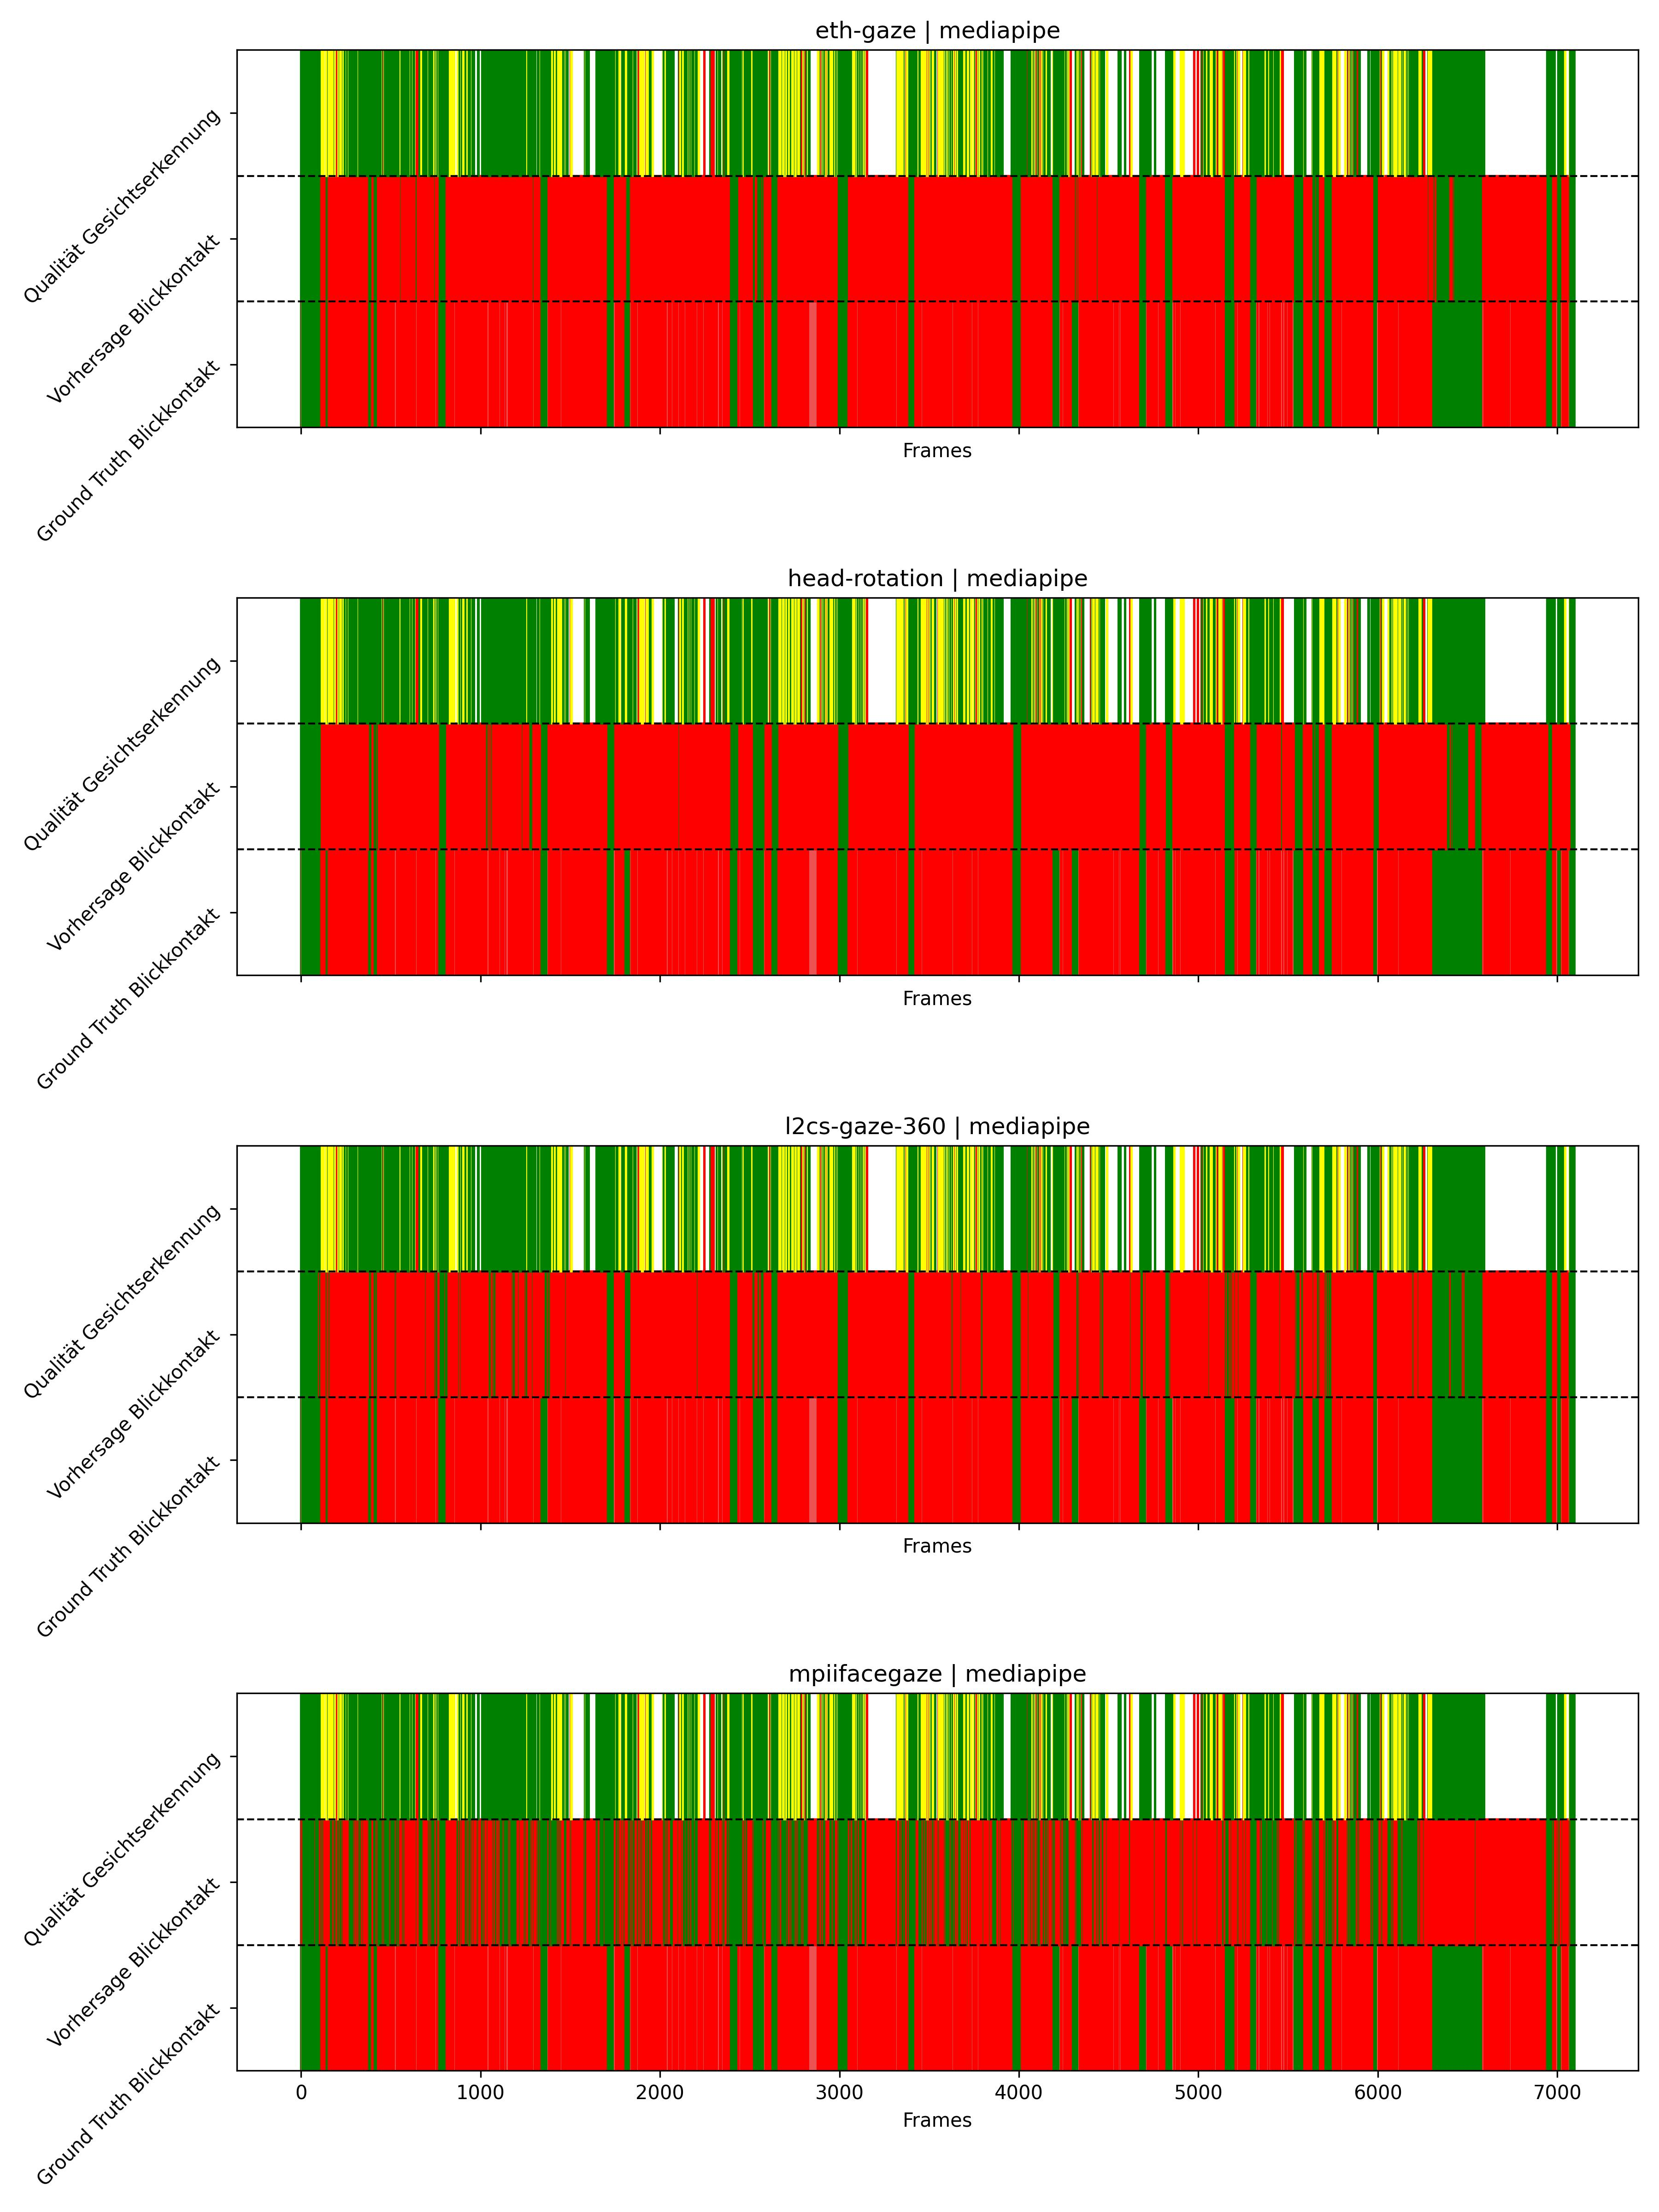
\includegraphics[width=1\linewidth]{appendix/11-mediapipe-overview-gaze.jpg}
\caption{Überblick über die Ground Truth des Blickkontakts, die Vorhersage des Blickkontakts und die Qualität der Gesichtserkennung mit \mediapipe. Die Bedeutung der Farben ist in Abbildung \ref{fig:evaluation:gaze:mpiifacegaze} erklärt.}
\end{figure}

\section{Video 12}
\begin{figure}[H]
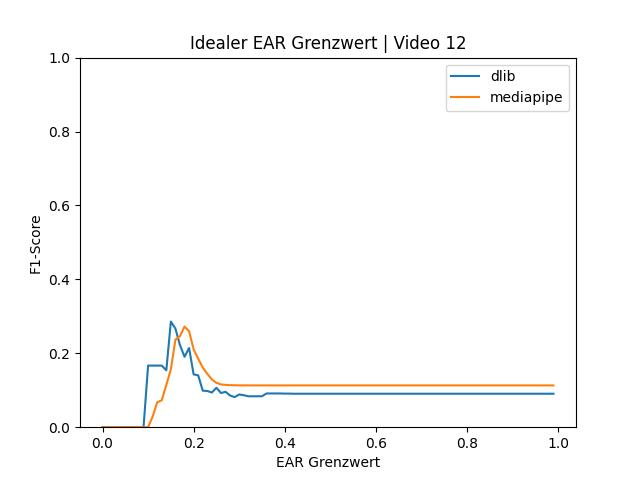
\includegraphics[width=0.7\linewidth]{appendix/12_f1-score-blink.jpg}
\caption{Ergebnisse der Bestimmung des idealen EAR-Grenzwerts für Video 12.}
\end{figure}

\begin{figure}[H]
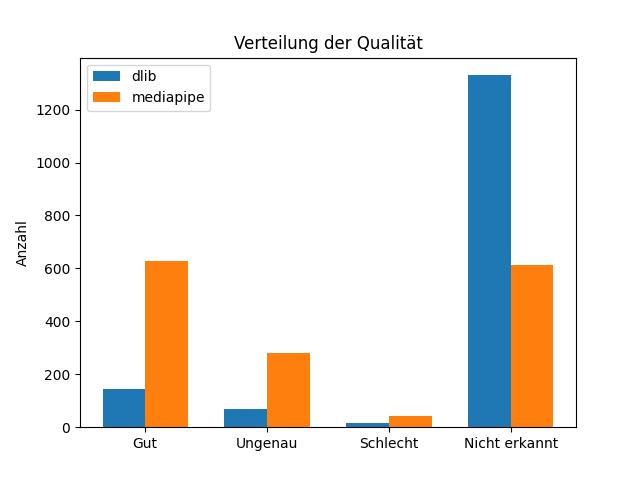
\includegraphics[width=0.7\linewidth]{appendix/12_bar-quality.jpg}
\caption{Aufteilung der Gesichtserkennungsqualität von Video 12.}
\end{figure}

\begin{table}[H]
\centering
\begin{tabular}{l|l|c c |c}
\toprule
\textbf{Gesichtserkennung} & \textbf{Blickrichtung} & \textbf{Seitenlänge} $\hitthresholdsize$ & \textbf{Verschiebung} $\hitthresholdposition$ & \textbf{F1-Score} \\ 
\midrule
\multirow{4}*{dlib}& ETH-XGaze & 0,224 & -0,002 & 0,966  \\ 
& Gaze360 & 0,306 & 0,035 & 0,917 \\ 
& MPIIFaceGaze & 0,051 & -0,027 & 0,774  \\ 
& Kopfrotation & 0,255 & 0,194 & 0,787  \\ 
\hline\multirow{4}*{MediaPipe}& ETH-XGaze & 0,255 & -0,002 & 0,981  \\ 
& Gaze360 & 0,367 & 0,035 & 0,815 \\ 
& MPIIFaceGaze & 0,02 & -0,039 & 0,428  \\ 
& Kopfrotation & 0,194 & 0,194 & 0,899  \\ 
\bottomrule\end{tabular}
\caption{Ergebnis des Hyperparameter-Tunings für die Zone speziell für Video 12.}
\label{tab:appendix:12:local}
\end{table}
\begin{table}[H]
\centering
\begin{tabular}{l|l|c c c c|c c|c}
\toprule
\textbf{Gesichtserkennung} & \textbf{Blickrichtung} & $TP$ & $TN$& $FP$ & $FN$ & \textbf{Precision} & \textbf{Recall} & \textbf{F1-Score} \\ 
\midrule
\multirow{4}*{dlib}& ETH-XGaze & 125 & 1424 & 6 & 7 & 0,954 & 0,947 & 0,951 \\ 
& Gaze360 & 120 & 1417 & 13 & 12 & 0,902 & 0,909 & 0,906 \\ 
& MPIIFaceGaze & 123 & 1362 & 68 & 9 & 0,644 & 0,932 & 0,762 \\ 
& Kopfrotation & 126 & 1360 & 70 & 6 & 0,643 & 0,955 & 0,768 \\ 
\hline\multirow{4}*{MediaPipe}& ETH-XGaze & 132 & 1424 & 6 & 0 & 0,957 & 1,0 & 0,978 \\ 
& Gaze360 & 113 & 1387 & 43 & 19 & 0,724 & 0,856 & 0,785 \\ 
& MPIIFaceGaze & 125 & 888 & 542 & 7 & 0,187 & 0,947 & 0,313 \\ 
& Kopfrotation & 123 & 1408 & 22 & 9 & 0,848 & 0,932 & 0,888 \\ 
\bottomrule\end{tabular}
\caption{Zusammensetzung des F1-Scores unter Verwendung der in Kapitel \ref{sec:evaluation:results:gaze:threshold} bestimmten globalen Parameter $\hitthresholdsize$ und $\hitthresholdposition$.}
\label{tab:appendix:12:f1}
\end{table}
\begin{figure}[H]
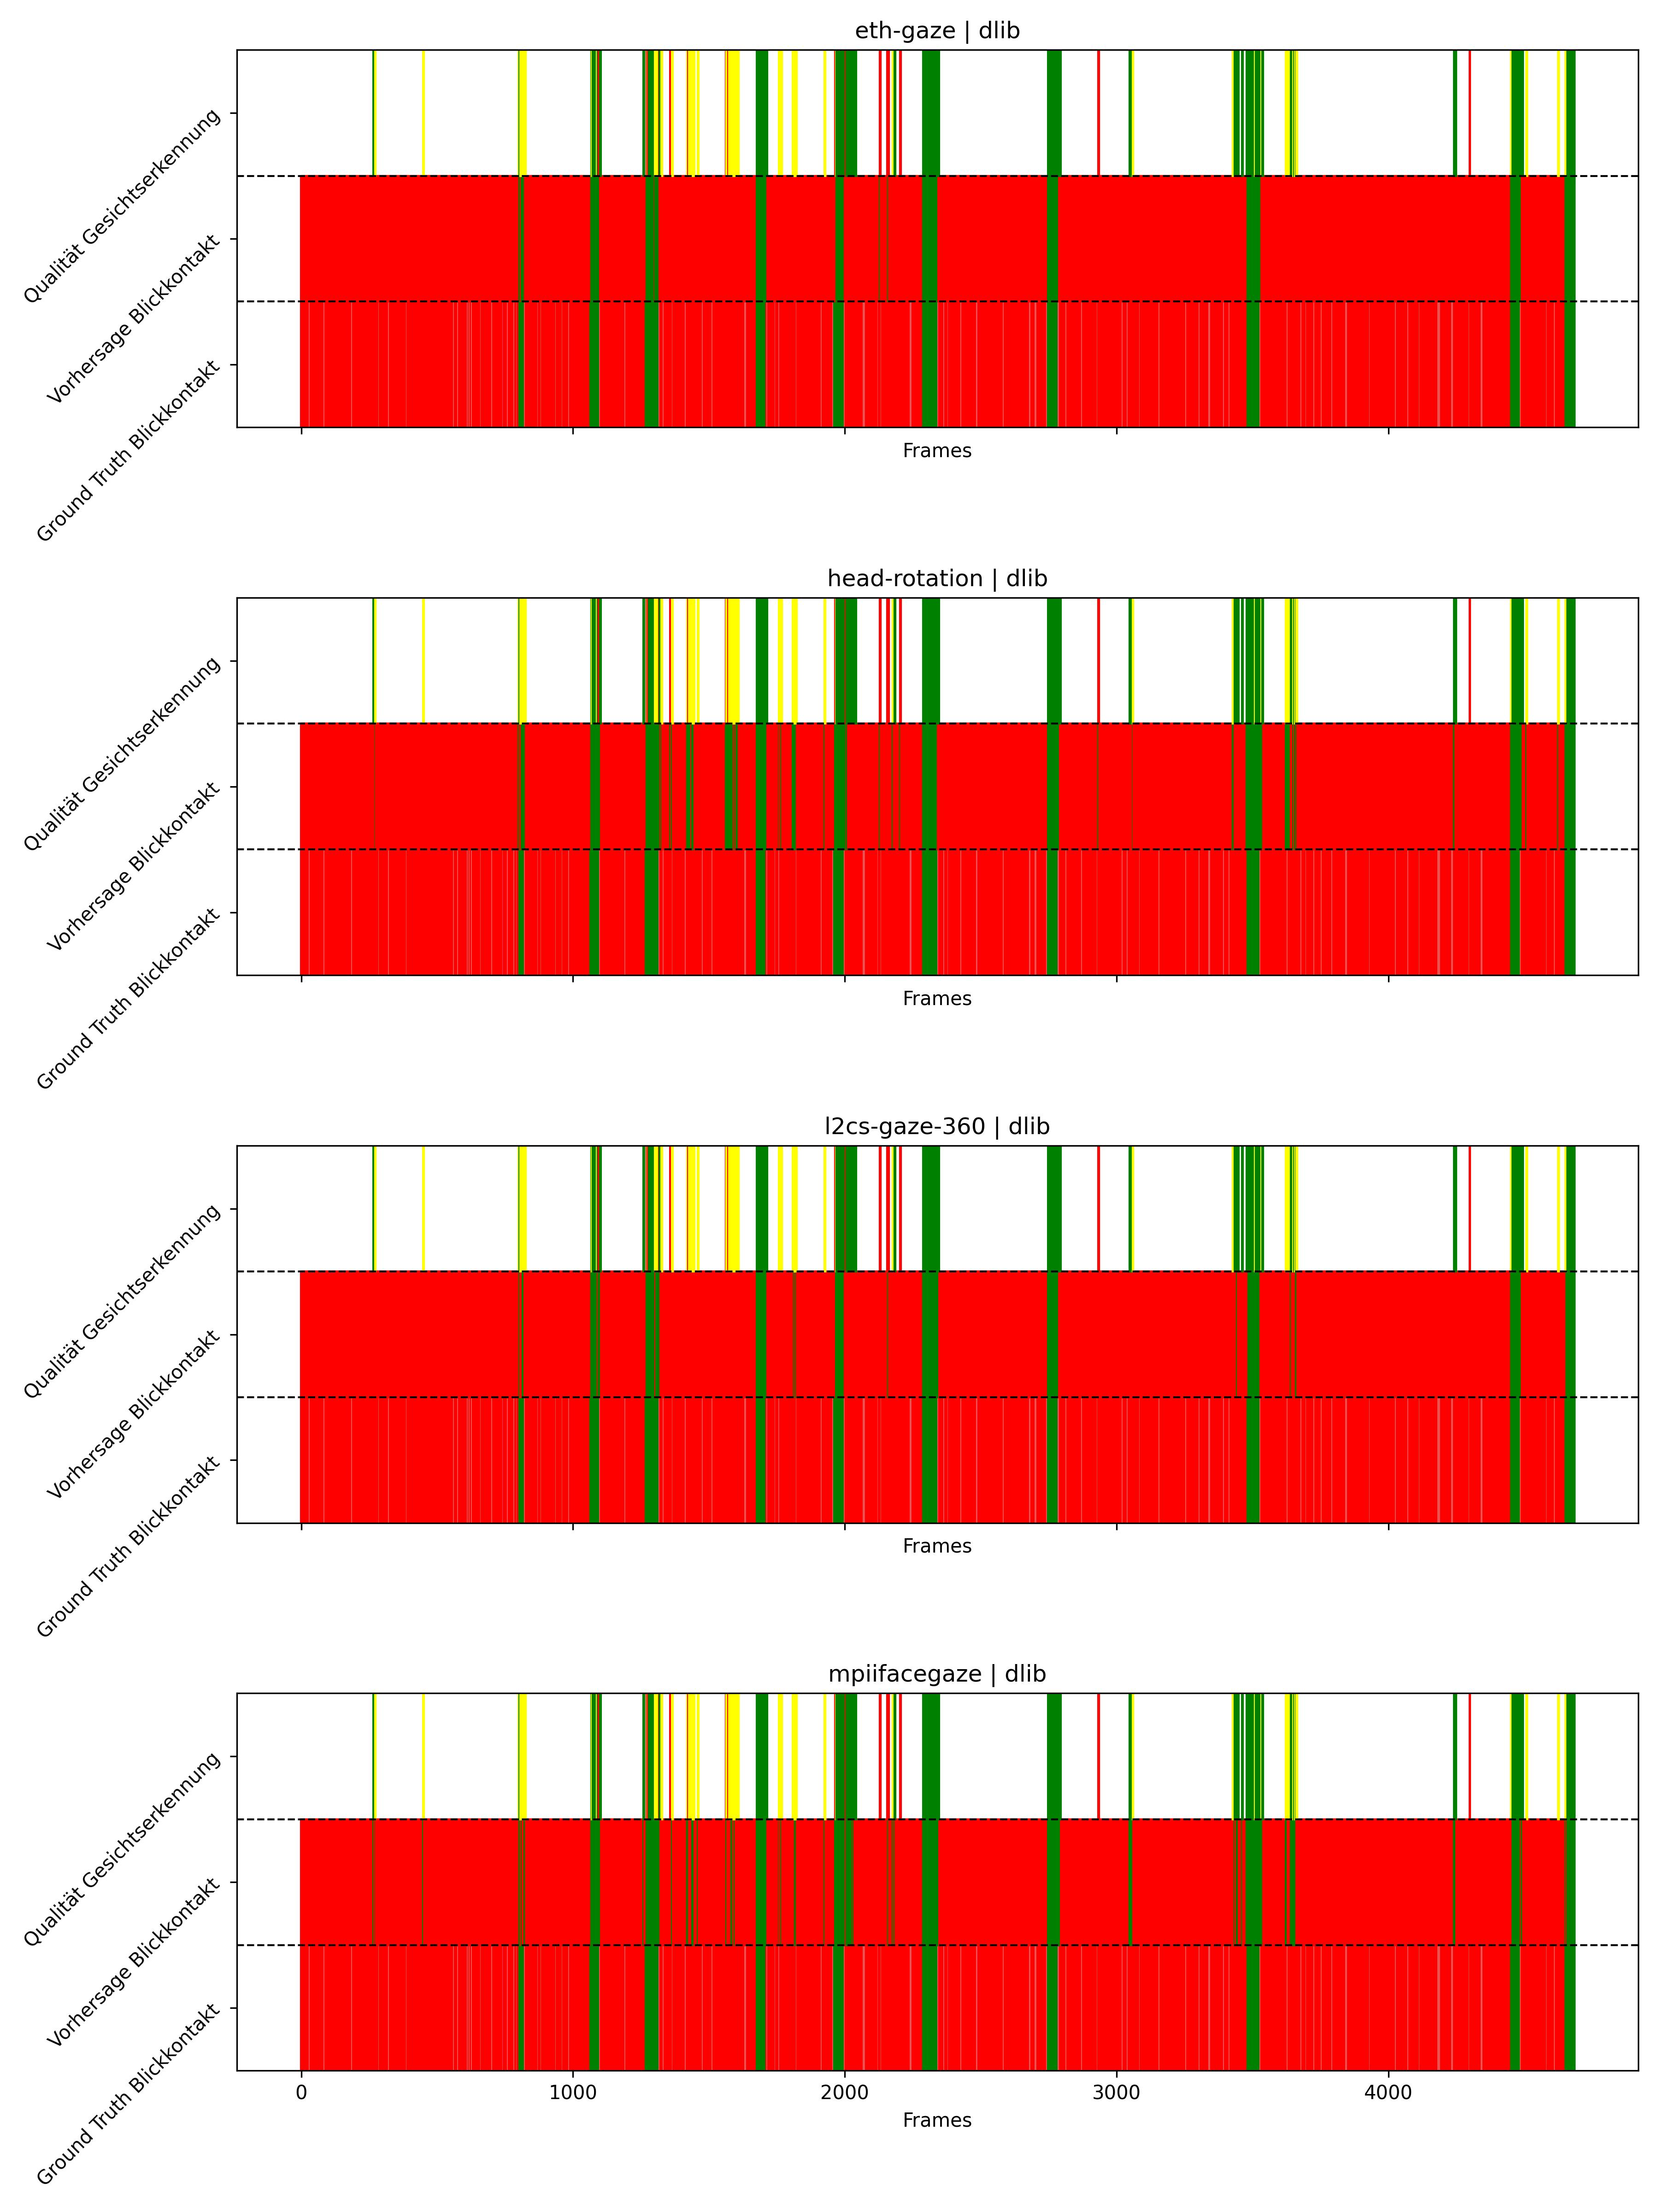
\includegraphics[width=1\linewidth]{appendix/12-dlib-overview-gaze.jpg}
\caption{Überblick über die Ground Truth des Blickkontakts, die Vorhersage des Blickkontakts und die Qualität der Gesichtserkennung mit \dlib. Die Bedeutung der Farben ist in Abbildung \ref{fig:evaluation:gaze:mpiifacegaze} erklärt.  }
\end{figure}

\begin{figure}[H]
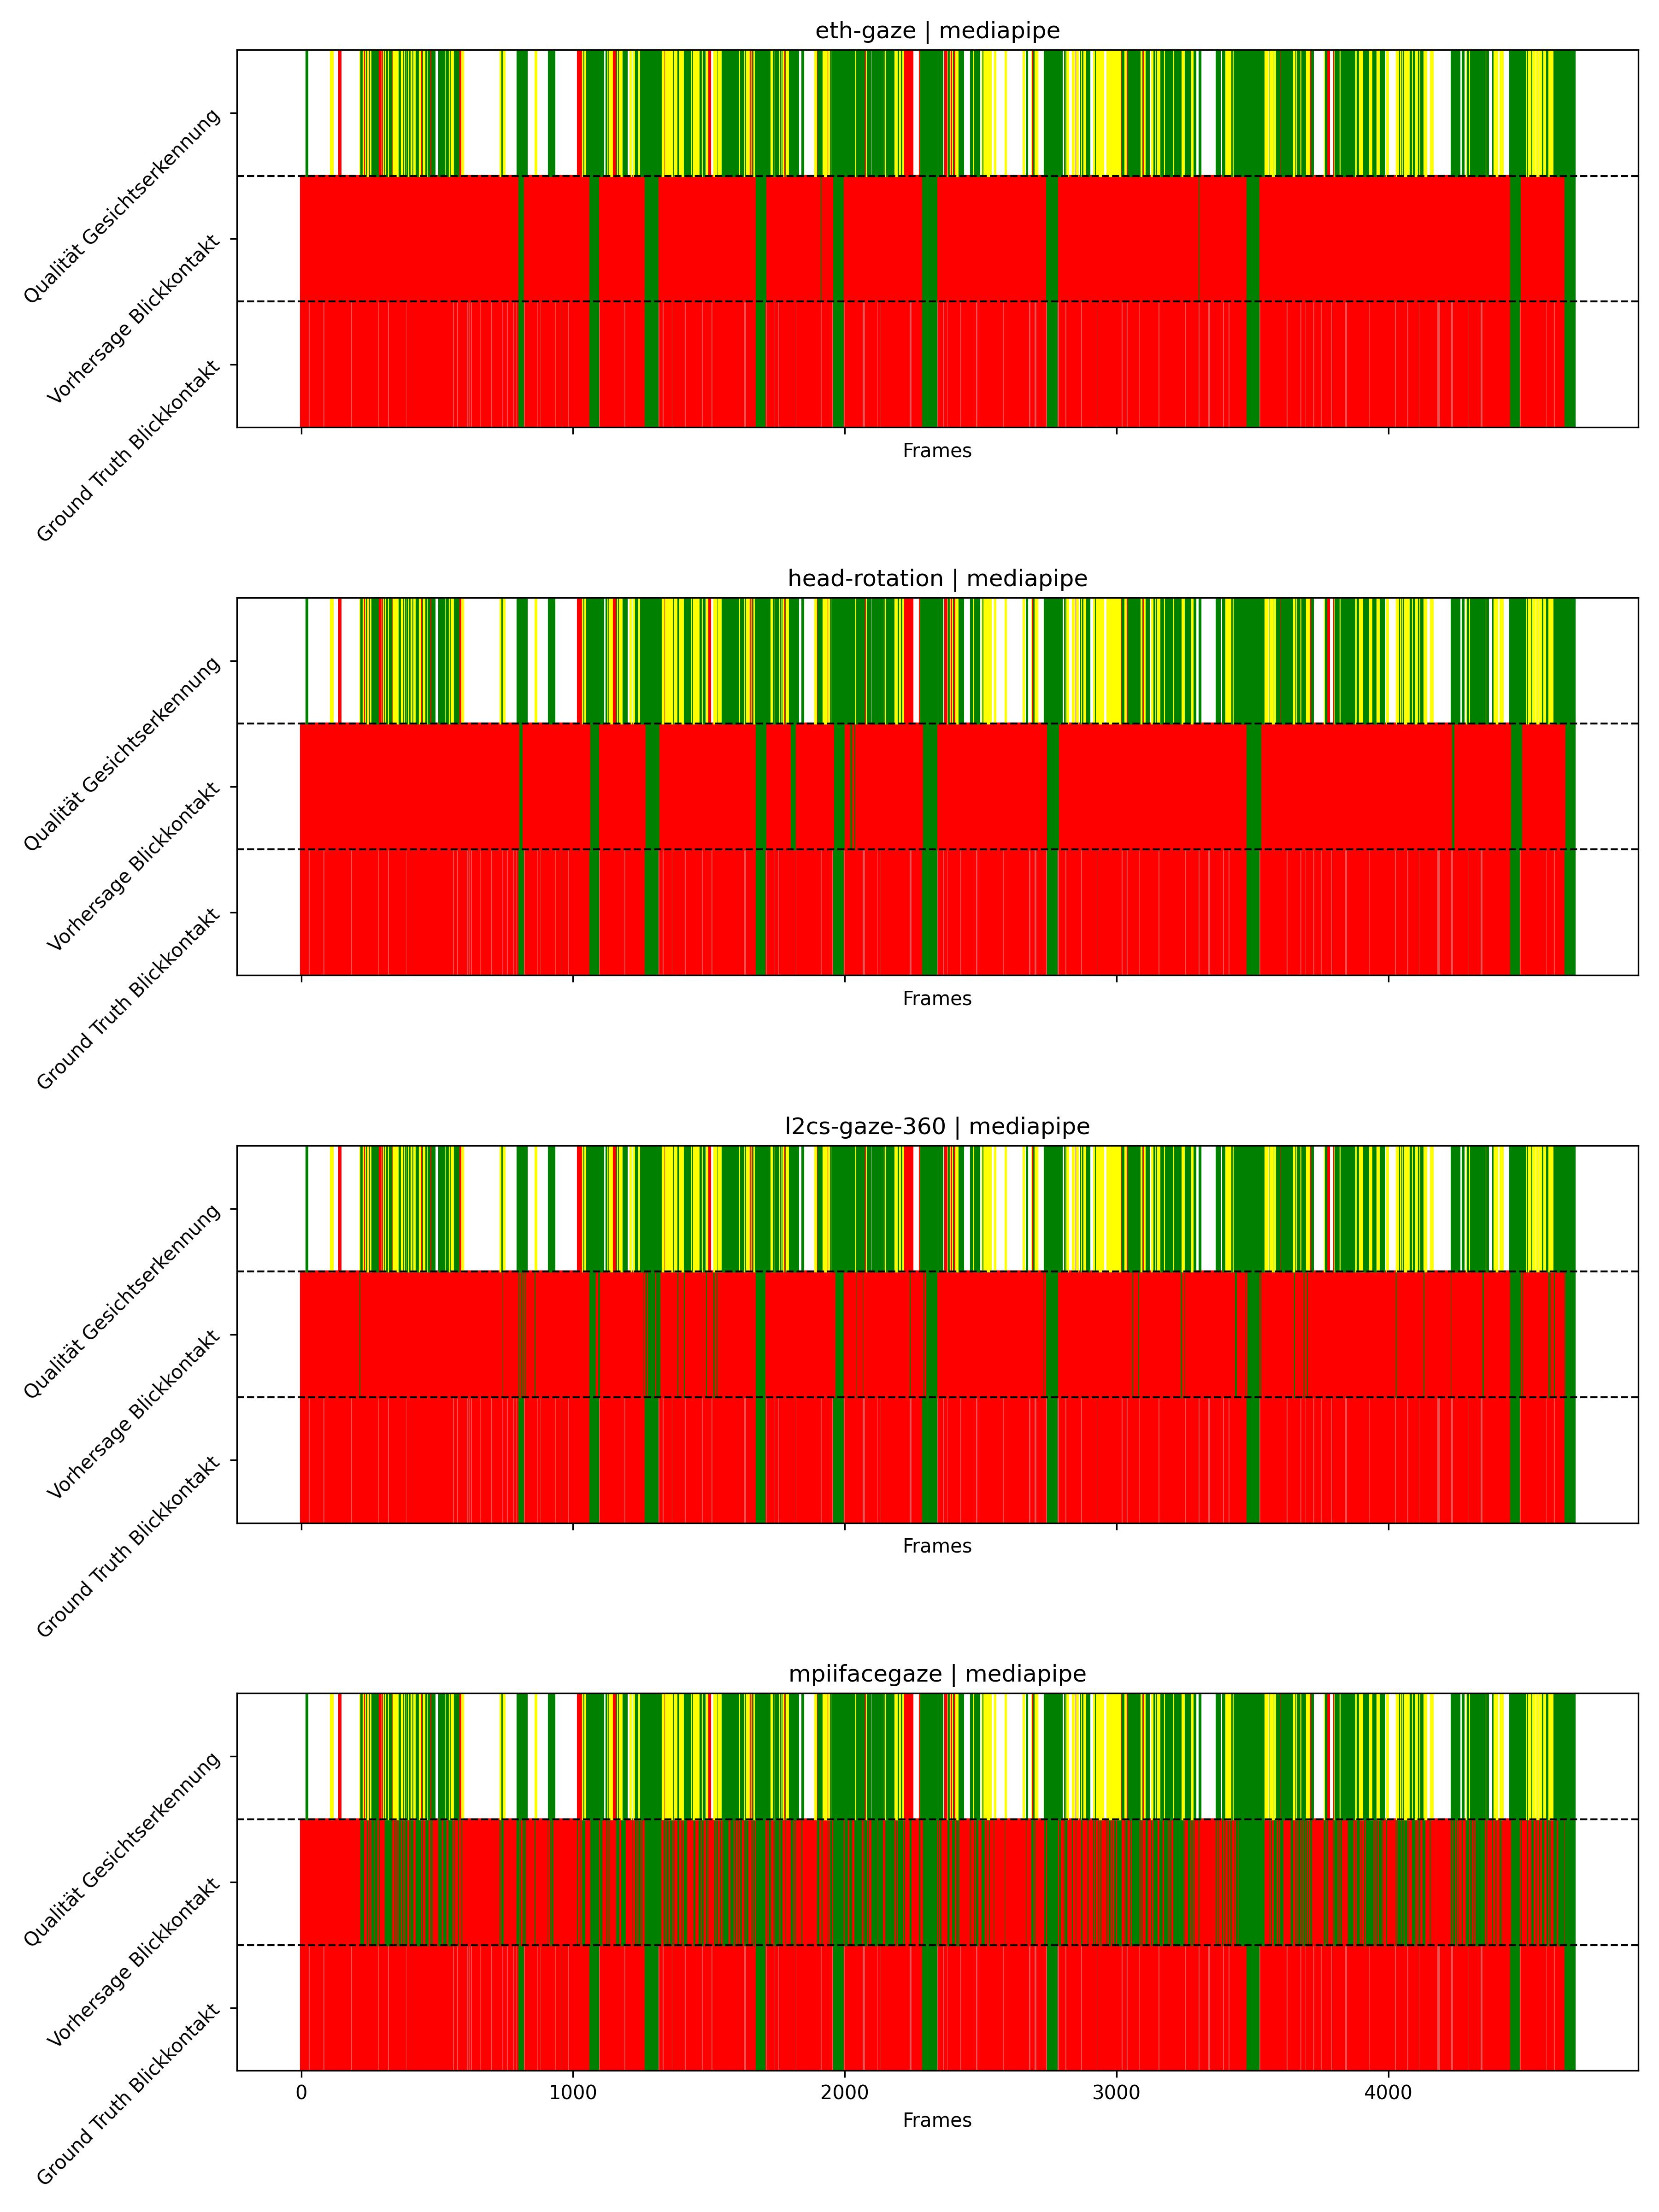
\includegraphics[width=1\linewidth]{appendix/12-mediapipe-overview-gaze.jpg}
\caption{Überblick über die Ground Truth des Blickkontakts, die Vorhersage des Blickkontakts und die Qualität der Gesichtserkennung mit \mediapipe. Die Bedeutung der Farben ist in Abbildung \ref{fig:evaluation:gaze:mpiifacegaze} erklärt.}
\end{figure}

\section{Video 13}
\begin{figure}[H]
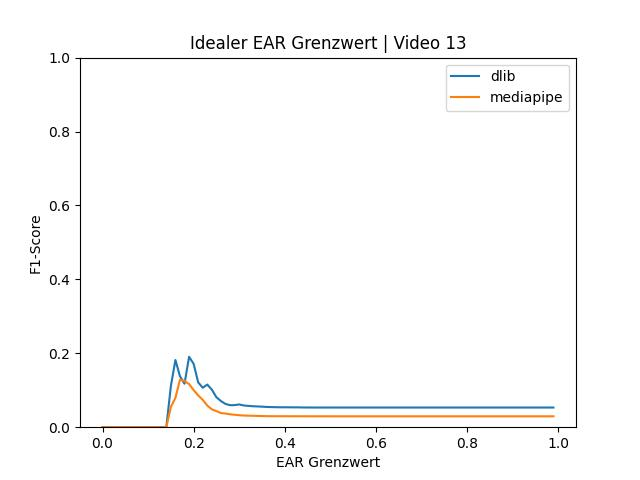
\includegraphics[width=0.7\linewidth]{appendix/13_f1-score-blink.jpg}
\caption{Ergebnisse der Bestimmung des idealen EAR-Grenzwerts für Video 13.}
\end{figure}

\begin{figure}[H]
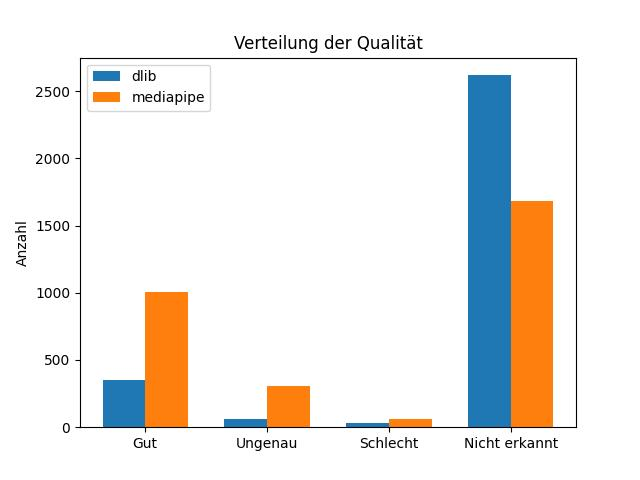
\includegraphics[width=0.7\linewidth]{appendix/13_bar-quality.jpg}
\caption{Aufteilung der Gesichtserkennungsqualität von Video 13.}
\end{figure}

\begin{table}[H]
\centering
\begin{tabular}{l|l|c c |c}
\toprule
\textbf{Gesichtserkennung} & \textbf{Blickrichtung} & \textbf{Seitenlänge} $\hitthresholdsize$ & \textbf{Verschiebung} $\hitthresholdposition$ & \textbf{F1-Score} \\ 
\midrule
\multirow{4}*{dlib}& ETH-XGaze & 0,194 & -0,002 & 0,929  \\ 
& Gaze360 & 0,224 & 0,071 & 0,885 \\ 
& MPIIFaceGaze & 0,082 & -0,027 & 0,827  \\ 
& Kopfrotation & 0,316 & 0,206 & 0,84  \\ 
\hline\multirow{4}*{MediaPipe}& ETH-XGaze & 0,184 & -0,002 & 0,977  \\ 
& Gaze360 & 0,378 & 0,047 & 0,875 \\ 
& MPIIFaceGaze & 0,041 & -0,027 & 0,478  \\ 
& Kopfrotation & 0,357 & 0,206 & 0,932  \\ 
\bottomrule\end{tabular}
\caption{Ergebnis des Hyperparameter-Tunings für die Zone speziell für Video 13.}
\label{tab:appendix:13:local}
\end{table}
\begin{table}[H]
\centering
\begin{tabular}{l|l|c c c c|c c|c}
\toprule
\textbf{Gesichtserkennung} & \textbf{Blickrichtung} & $TP$ & $TN$& $FP$ & $FN$ & \textbf{Precision} & \textbf{Recall} & \textbf{F1-Score} \\ 
\midrule
\multirow{4}*{dlib}& ETH-XGaze & 321 & 2680 & 9 & 45 & 0,973 & 0,877 & 0,922 \\ 
& Gaze360 & 314 & 2658 & 31 & 52 & 0,91 & 0,858 & 0,883 \\ 
& MPIIFaceGaze & 317 & 2604 & 85 & 49 & 0,789 & 0,866 & 0,826 \\ 
& Kopfrotation & 307 & 2621 & 68 & 59 & 0,819 & 0,839 & 0,829 \\ 
\hline\multirow{4}*{MediaPipe}& ETH-XGaze & 363 & 2660 & 32 & 3 & 0,919 & 0,992 & 0,954 \\ 
& Gaze360 & 348 & 2610 & 82 & 18 & 0,809 & 0,951 & 0,874 \\ 
& MPIIFaceGaze & 290 & 2091 & 601 & 76 & 0,325 & 0,792 & 0,461 \\ 
& Kopfrotation & 316 & 2659 & 33 & 50 & 0,905 & 0,863 & 0,884 \\ 
\bottomrule\end{tabular}
\caption{Zusammensetzung des F1-Scores unter Verwendung der in Kapitel \ref{sec:evaluation:results:gaze:threshold} bestimmten globalen Parameter $\hitthresholdsize$ und $\hitthresholdposition$.}
\label{tab:appendix:13:f1}
\end{table}
\begin{figure}[H]
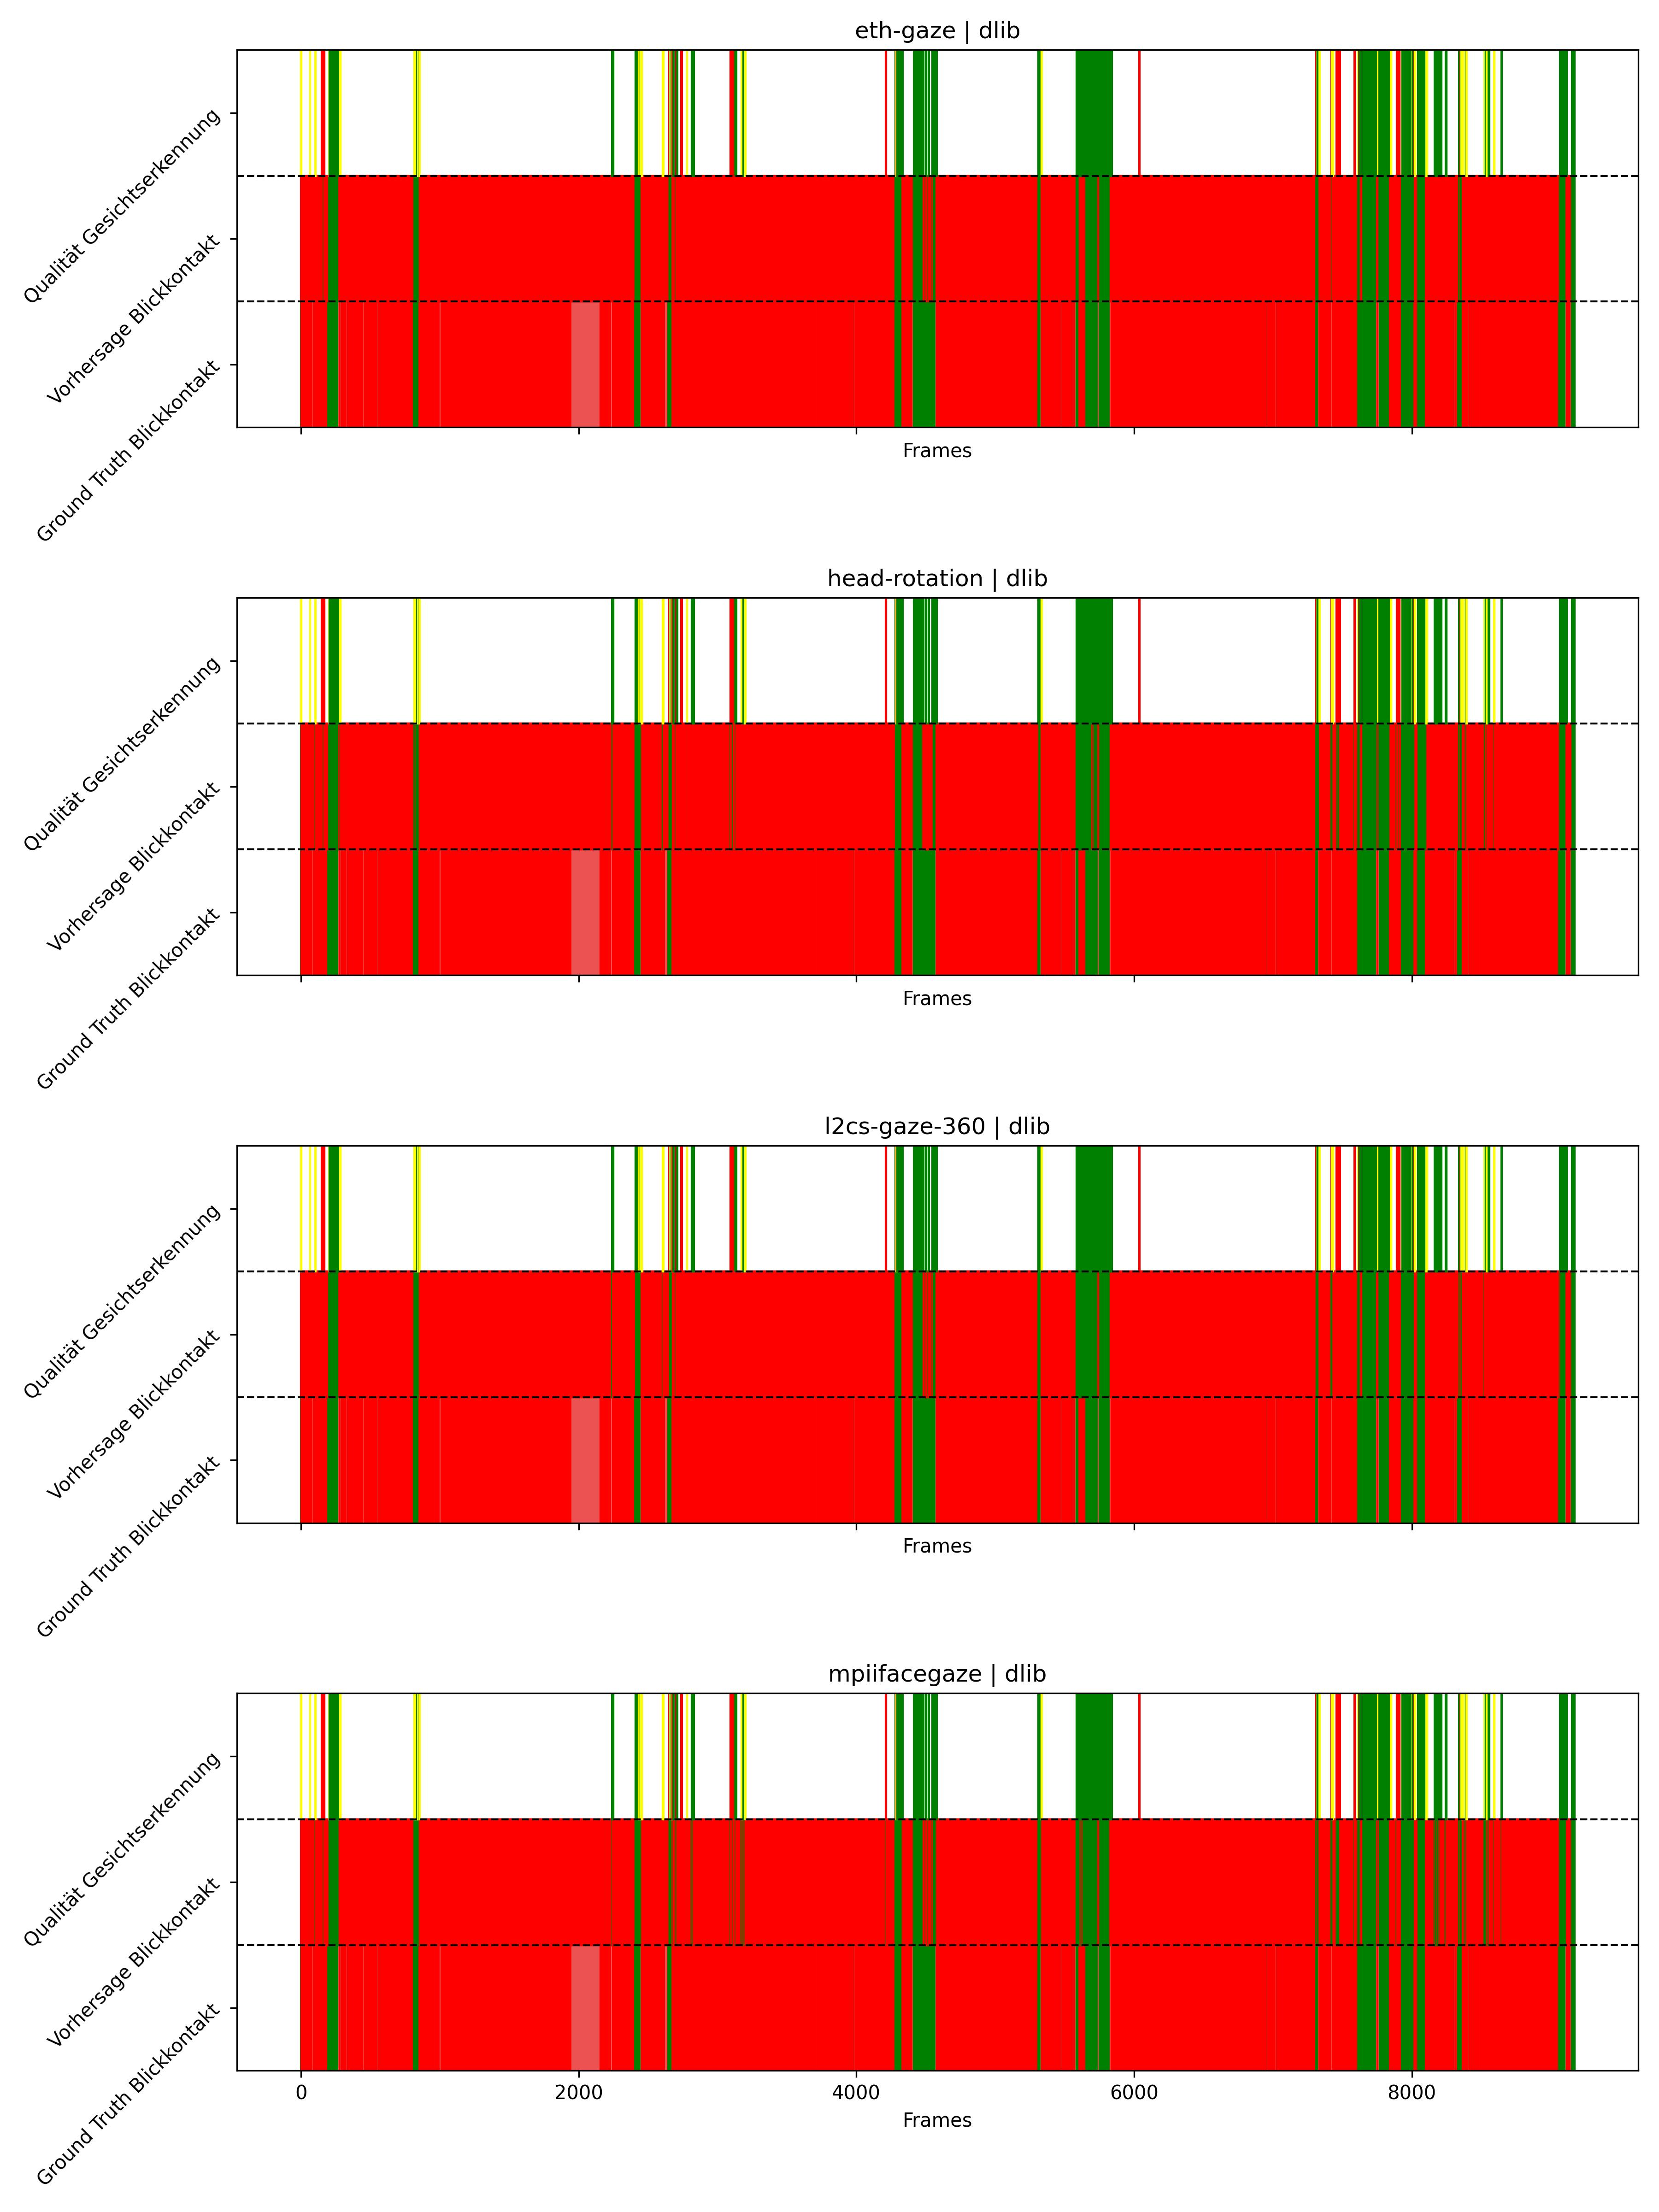
\includegraphics[width=1\linewidth]{appendix/13-dlib-overview-gaze.jpg}
\caption{Überblick über die Ground Truth des Blickkontakts, die Vorhersage des Blickkontakts und die Qualität der Gesichtserkennung mit \dlib. Die Bedeutung der Farben ist in Abbildung \ref{fig:evaluation:gaze:mpiifacegaze} erklärt.  }
\end{figure}

\begin{figure}[H]
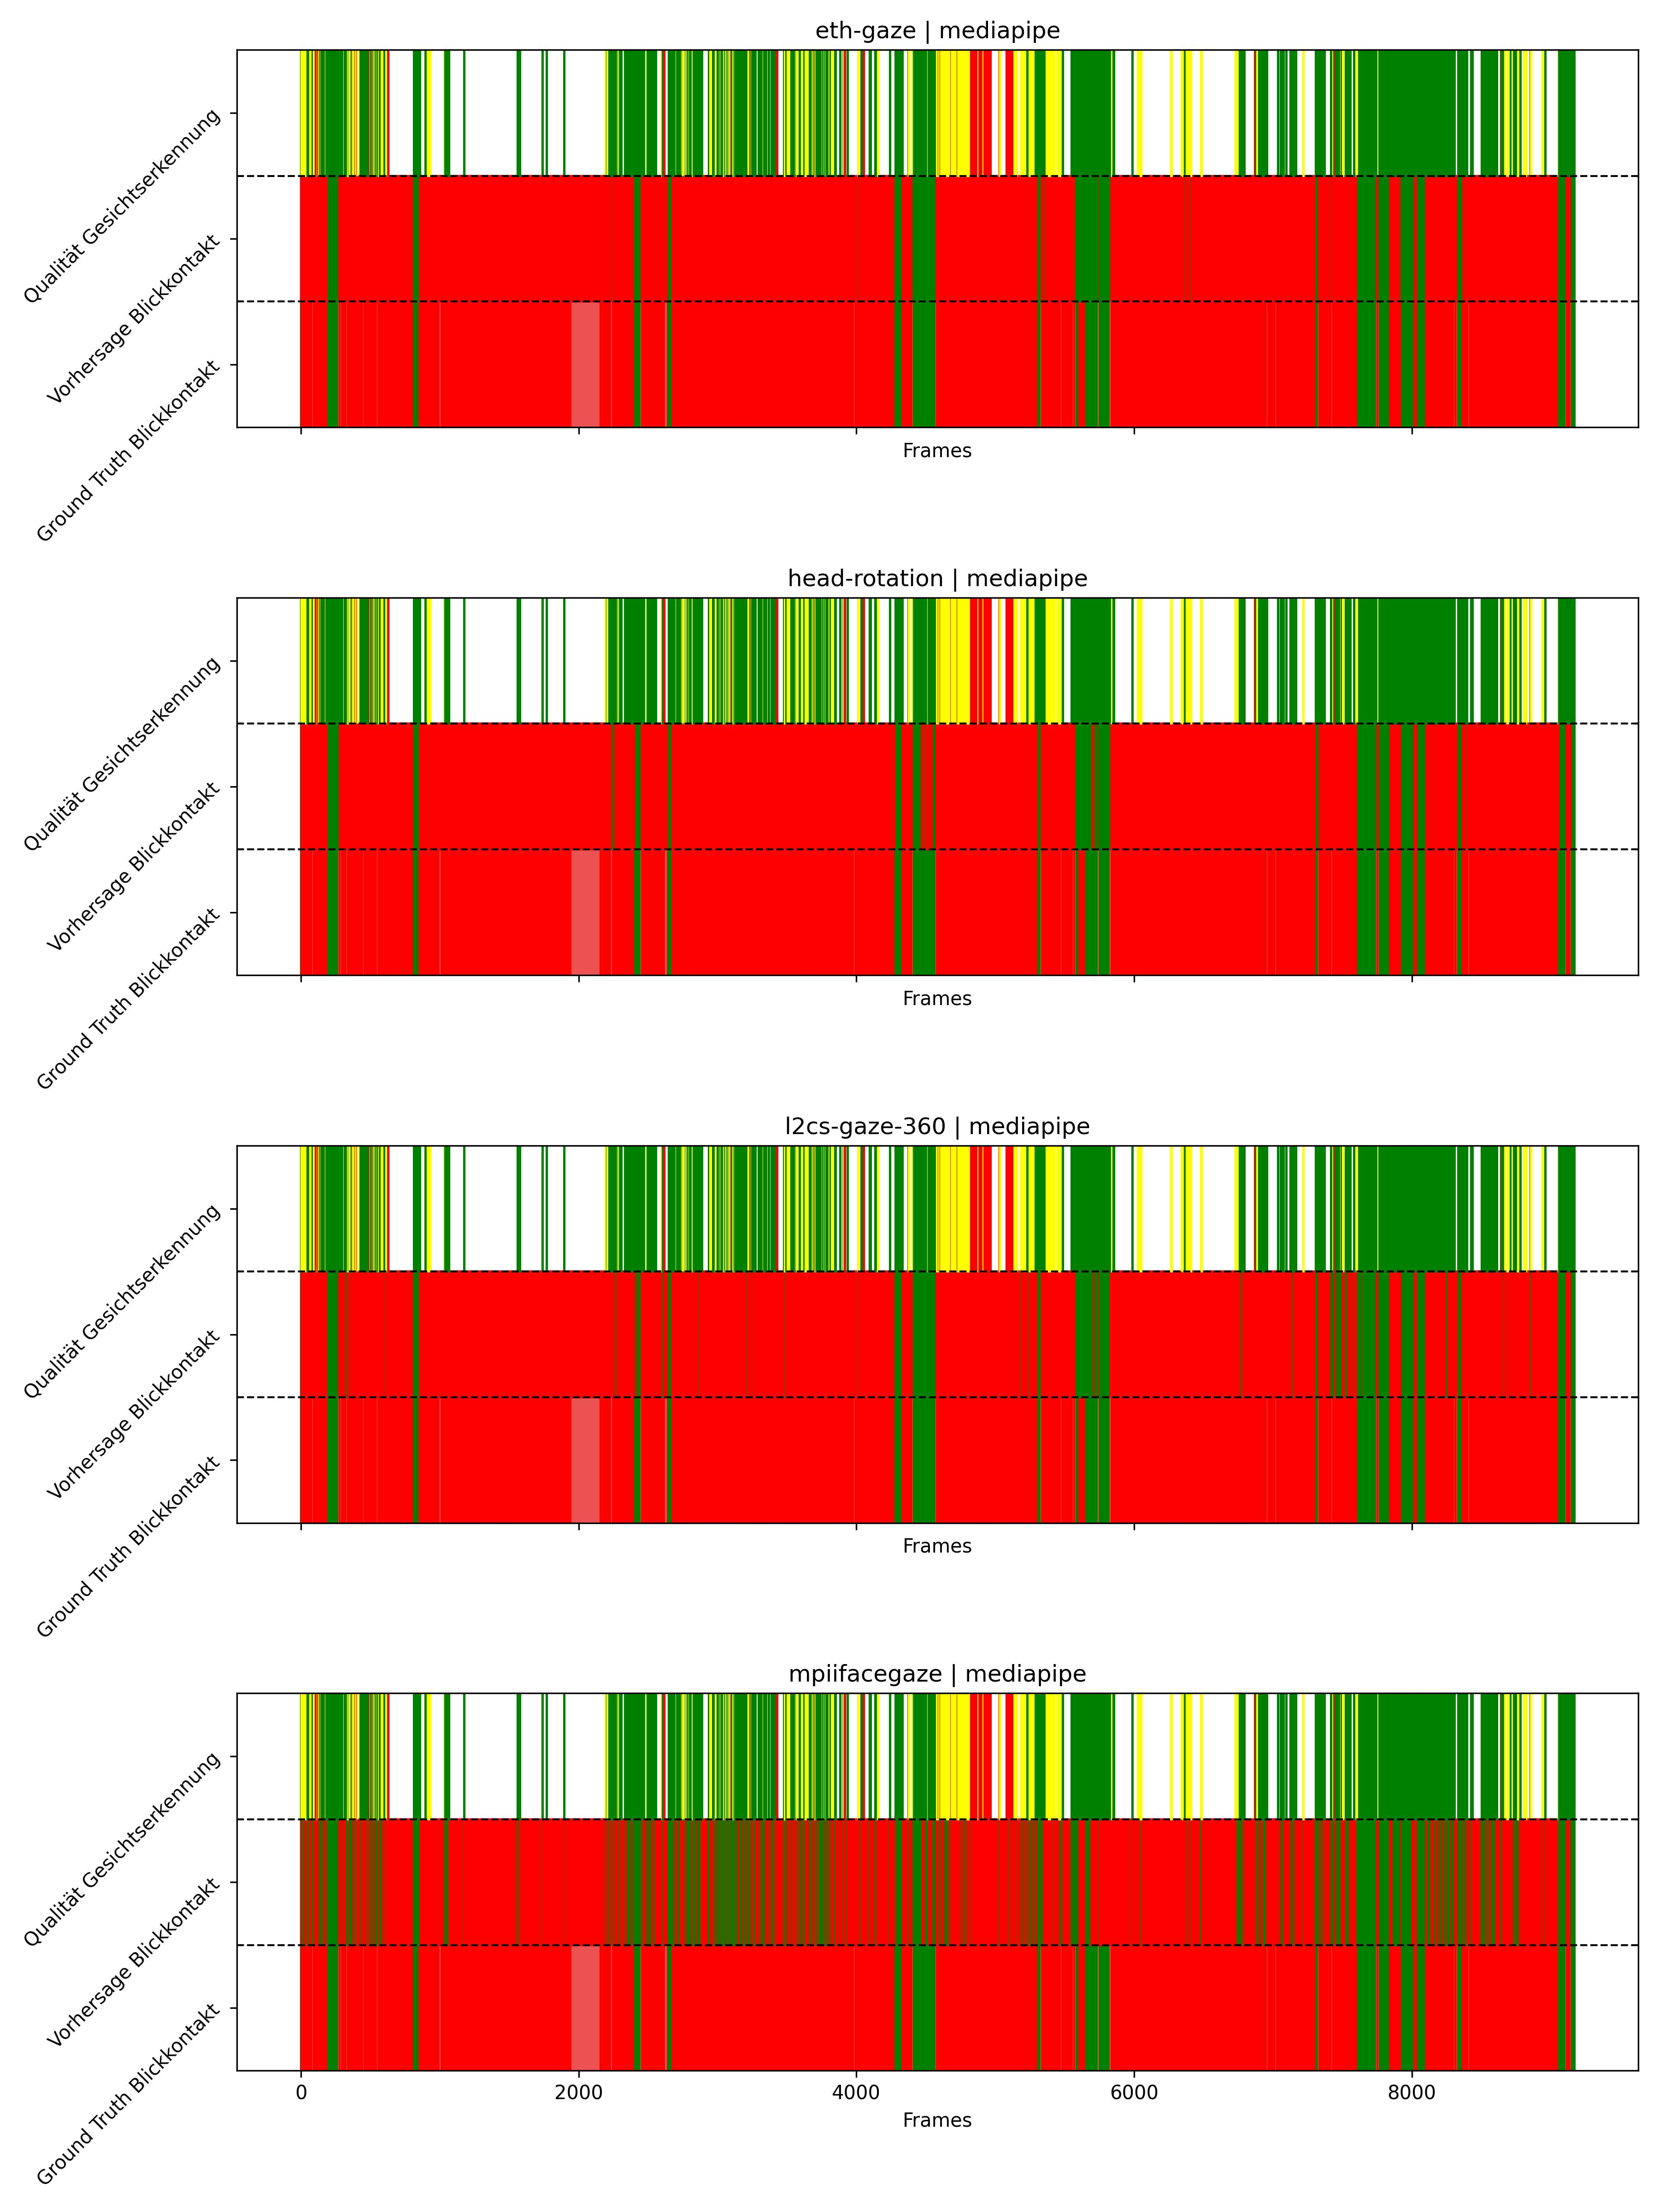
\includegraphics[width=1\linewidth]{appendix/13-mediapipe-overview-gaze.jpg}
\caption{Überblick über die Ground Truth des Blickkontakts, die Vorhersage des Blickkontakts und die Qualität der Gesichtserkennung mit \mediapipe. Die Bedeutung der Farben ist in Abbildung \ref{fig:evaluation:gaze:mpiifacegaze} erklärt.}
\end{figure}

\section{Video 14}
\begin{figure}[H]
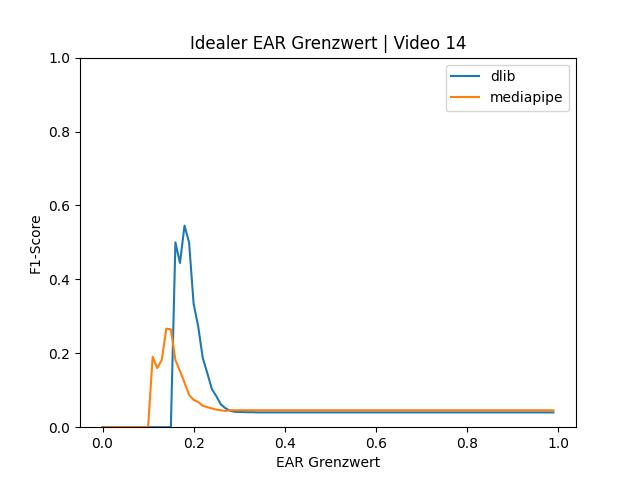
\includegraphics[width=0.7\linewidth]{appendix/14_f1-score-blink.jpg}
\caption{Ergebnisse der Bestimmung des idealen EAR-Grenzwerts für Video 14.}
\end{figure}

\begin{figure}[H]
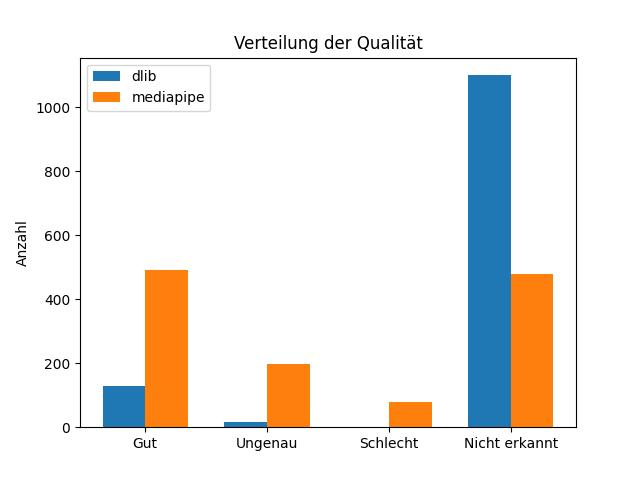
\includegraphics[width=0.7\linewidth]{appendix/14_bar-quality.jpg}
\caption{Aufteilung der Gesichtserkennungsqualität von Video 14.}
\end{figure}

\begin{table}[H]
\centering
\begin{tabular}{l|l|c c |c}
\toprule
\textbf{Gesichtserkennung} & \textbf{Blickrichtung} & \textbf{Seitenlänge} $\hitthresholdsize$ & \textbf{Verschiebung} $\hitthresholdposition$ & \textbf{F1-Score} \\ 
\midrule
\multirow{4}*{dlib}& ETH-XGaze & 0,204 & 0,01 & 0,756  \\ 
& Gaze360 & 0,347 & 0,047 & 0,75 \\ 
& MPIIFaceGaze & 0,061 & -0,014 & 0,709  \\ 
& Kopfrotation & 0,306 & 0,206 & 0,723  \\ 
\hline\multirow{4}*{MediaPipe}& ETH-XGaze & 0,163 & 0,047 & 0,925  \\ 
& Gaze360 & 0,48 & 0,035 & 0,737 \\ 
& MPIIFaceGaze & 0,092 & 0,035 & 0,458  \\ 
& Kopfrotation & 0,224 & 0,218 & 0,881  \\ 
\bottomrule\end{tabular}
\caption{Ergebnis des Hyperparameter-Tunings für die Zone speziell für Video 14.}
\label{tab:appendix:14:local}
\end{table}
\begin{table}[H]
\centering
\begin{tabular}{l|l|c c c c|c c|c}
\toprule
\textbf{Gesichtserkennung} & \textbf{Blickrichtung} & $TP$ & $TN$& $FP$ & $FN$ & \textbf{Precision} & \textbf{Recall} & \textbf{F1-Score} \\ 
\midrule
\multirow{4}*{dlib}& ETH-XGaze & 121 & 1046 & 1 & 78 & 0,992 & 0,608 & 0,754 \\ 
& Gaze360 & 120 & 1046 & 1 & 79 & 0,992 & 0,603 & 0,75 \\ 
& MPIIFaceGaze & 118 & 1026 & 21 & 81 & 0,849 & 0,593 & 0,698 \\ 
& Kopfrotation & 119 & 1034 & 13 & 80 & 0,902 & 0,598 & 0,719 \\ 
\hline\multirow{4}*{MediaPipe}& ETH-XGaze & 172 & 1048 & 1 & 27 & 0,994 & 0,864 & 0,925 \\ 
& Gaze360 & 122 & 1031 & 18 & 77 & 0,871 & 0,613 & 0,72 \\ 
& MPIIFaceGaze & 152 & 632 & 417 & 47 & 0,267 & 0,764 & 0,396 \\ 
& Kopfrotation & 164 & 1037 & 12 & 35 & 0,932 & 0,824 & 0,875 \\ 
\bottomrule\end{tabular}
\caption{Zusammensetzung des F1-Scores unter Verwendung der in Kapitel \ref{sec:evaluation:results:gaze:threshold} bestimmten globalen Parameter $\hitthresholdsize$ und $\hitthresholdposition$.}
\label{tab:appendix:14:f1}
\end{table}
\begin{figure}[H]
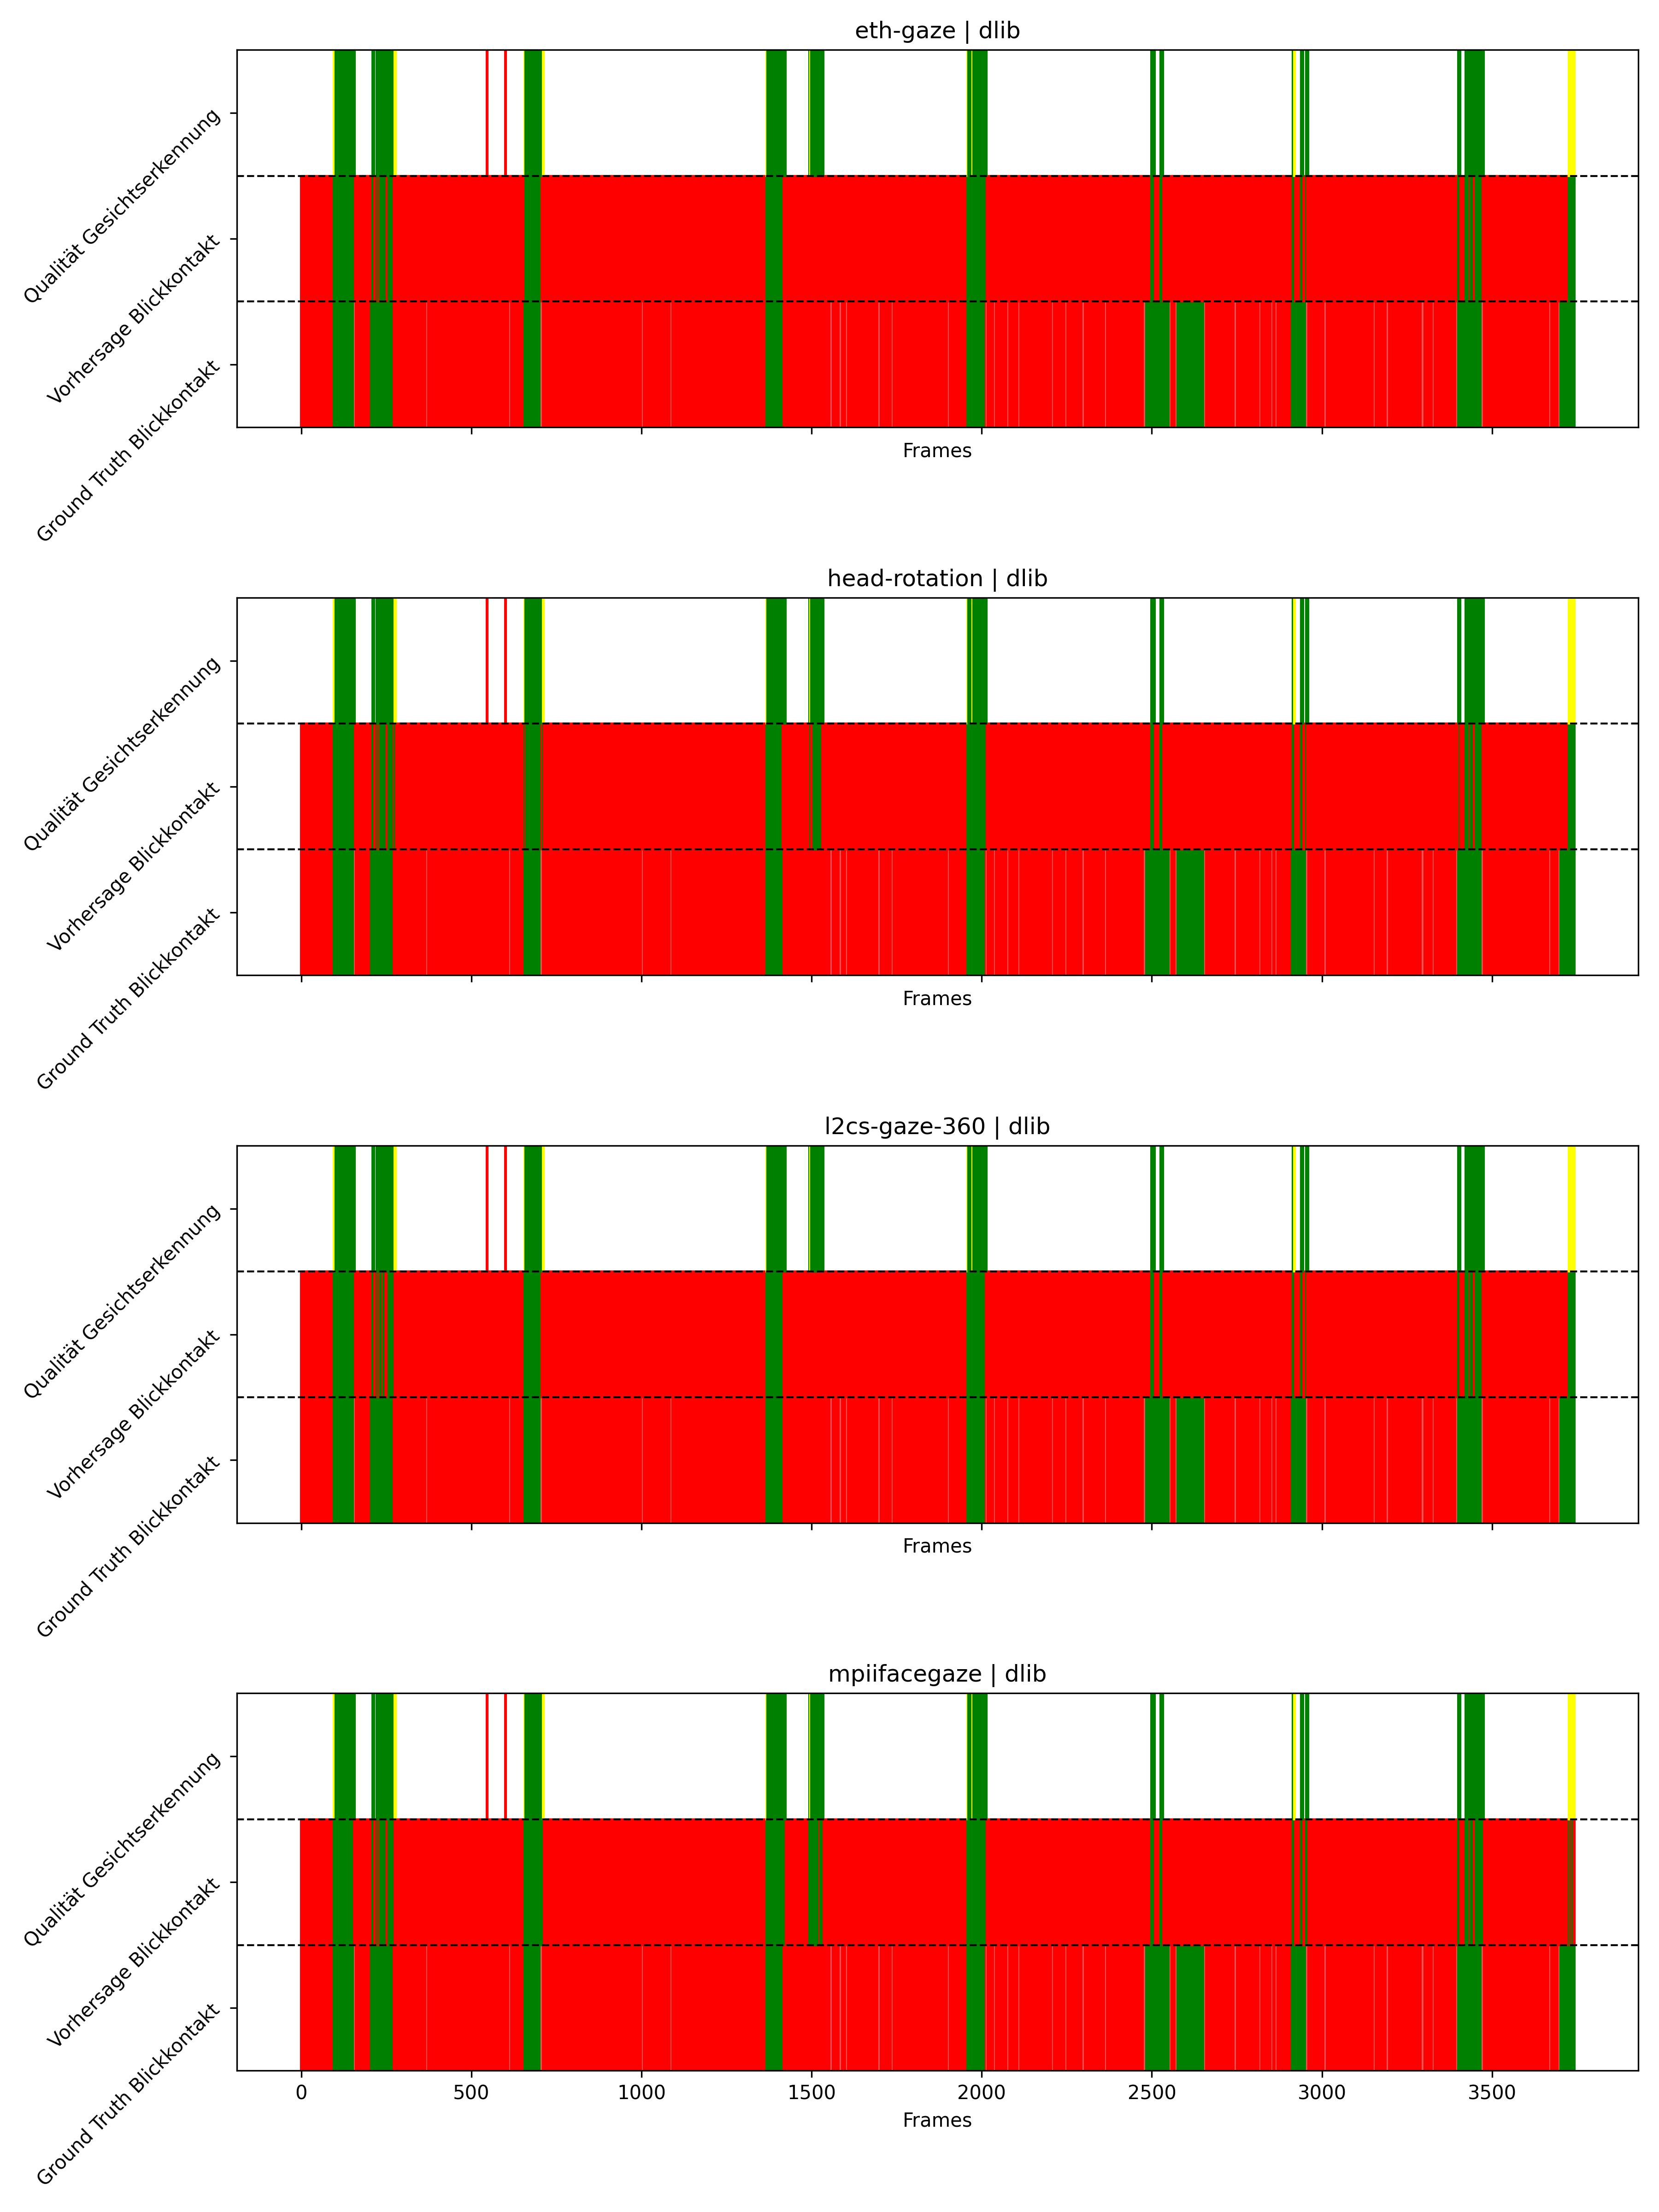
\includegraphics[width=1\linewidth]{appendix/14-dlib-overview-gaze.jpg}
\caption{Überblick über die Ground Truth des Blickkontakts, die Vorhersage des Blickkontakts und die Qualität der Gesichtserkennung mit \dlib. Die Bedeutung der Farben ist in Abbildung \ref{fig:evaluation:gaze:mpiifacegaze} erklärt.  }
\end{figure}

\begin{figure}[H]
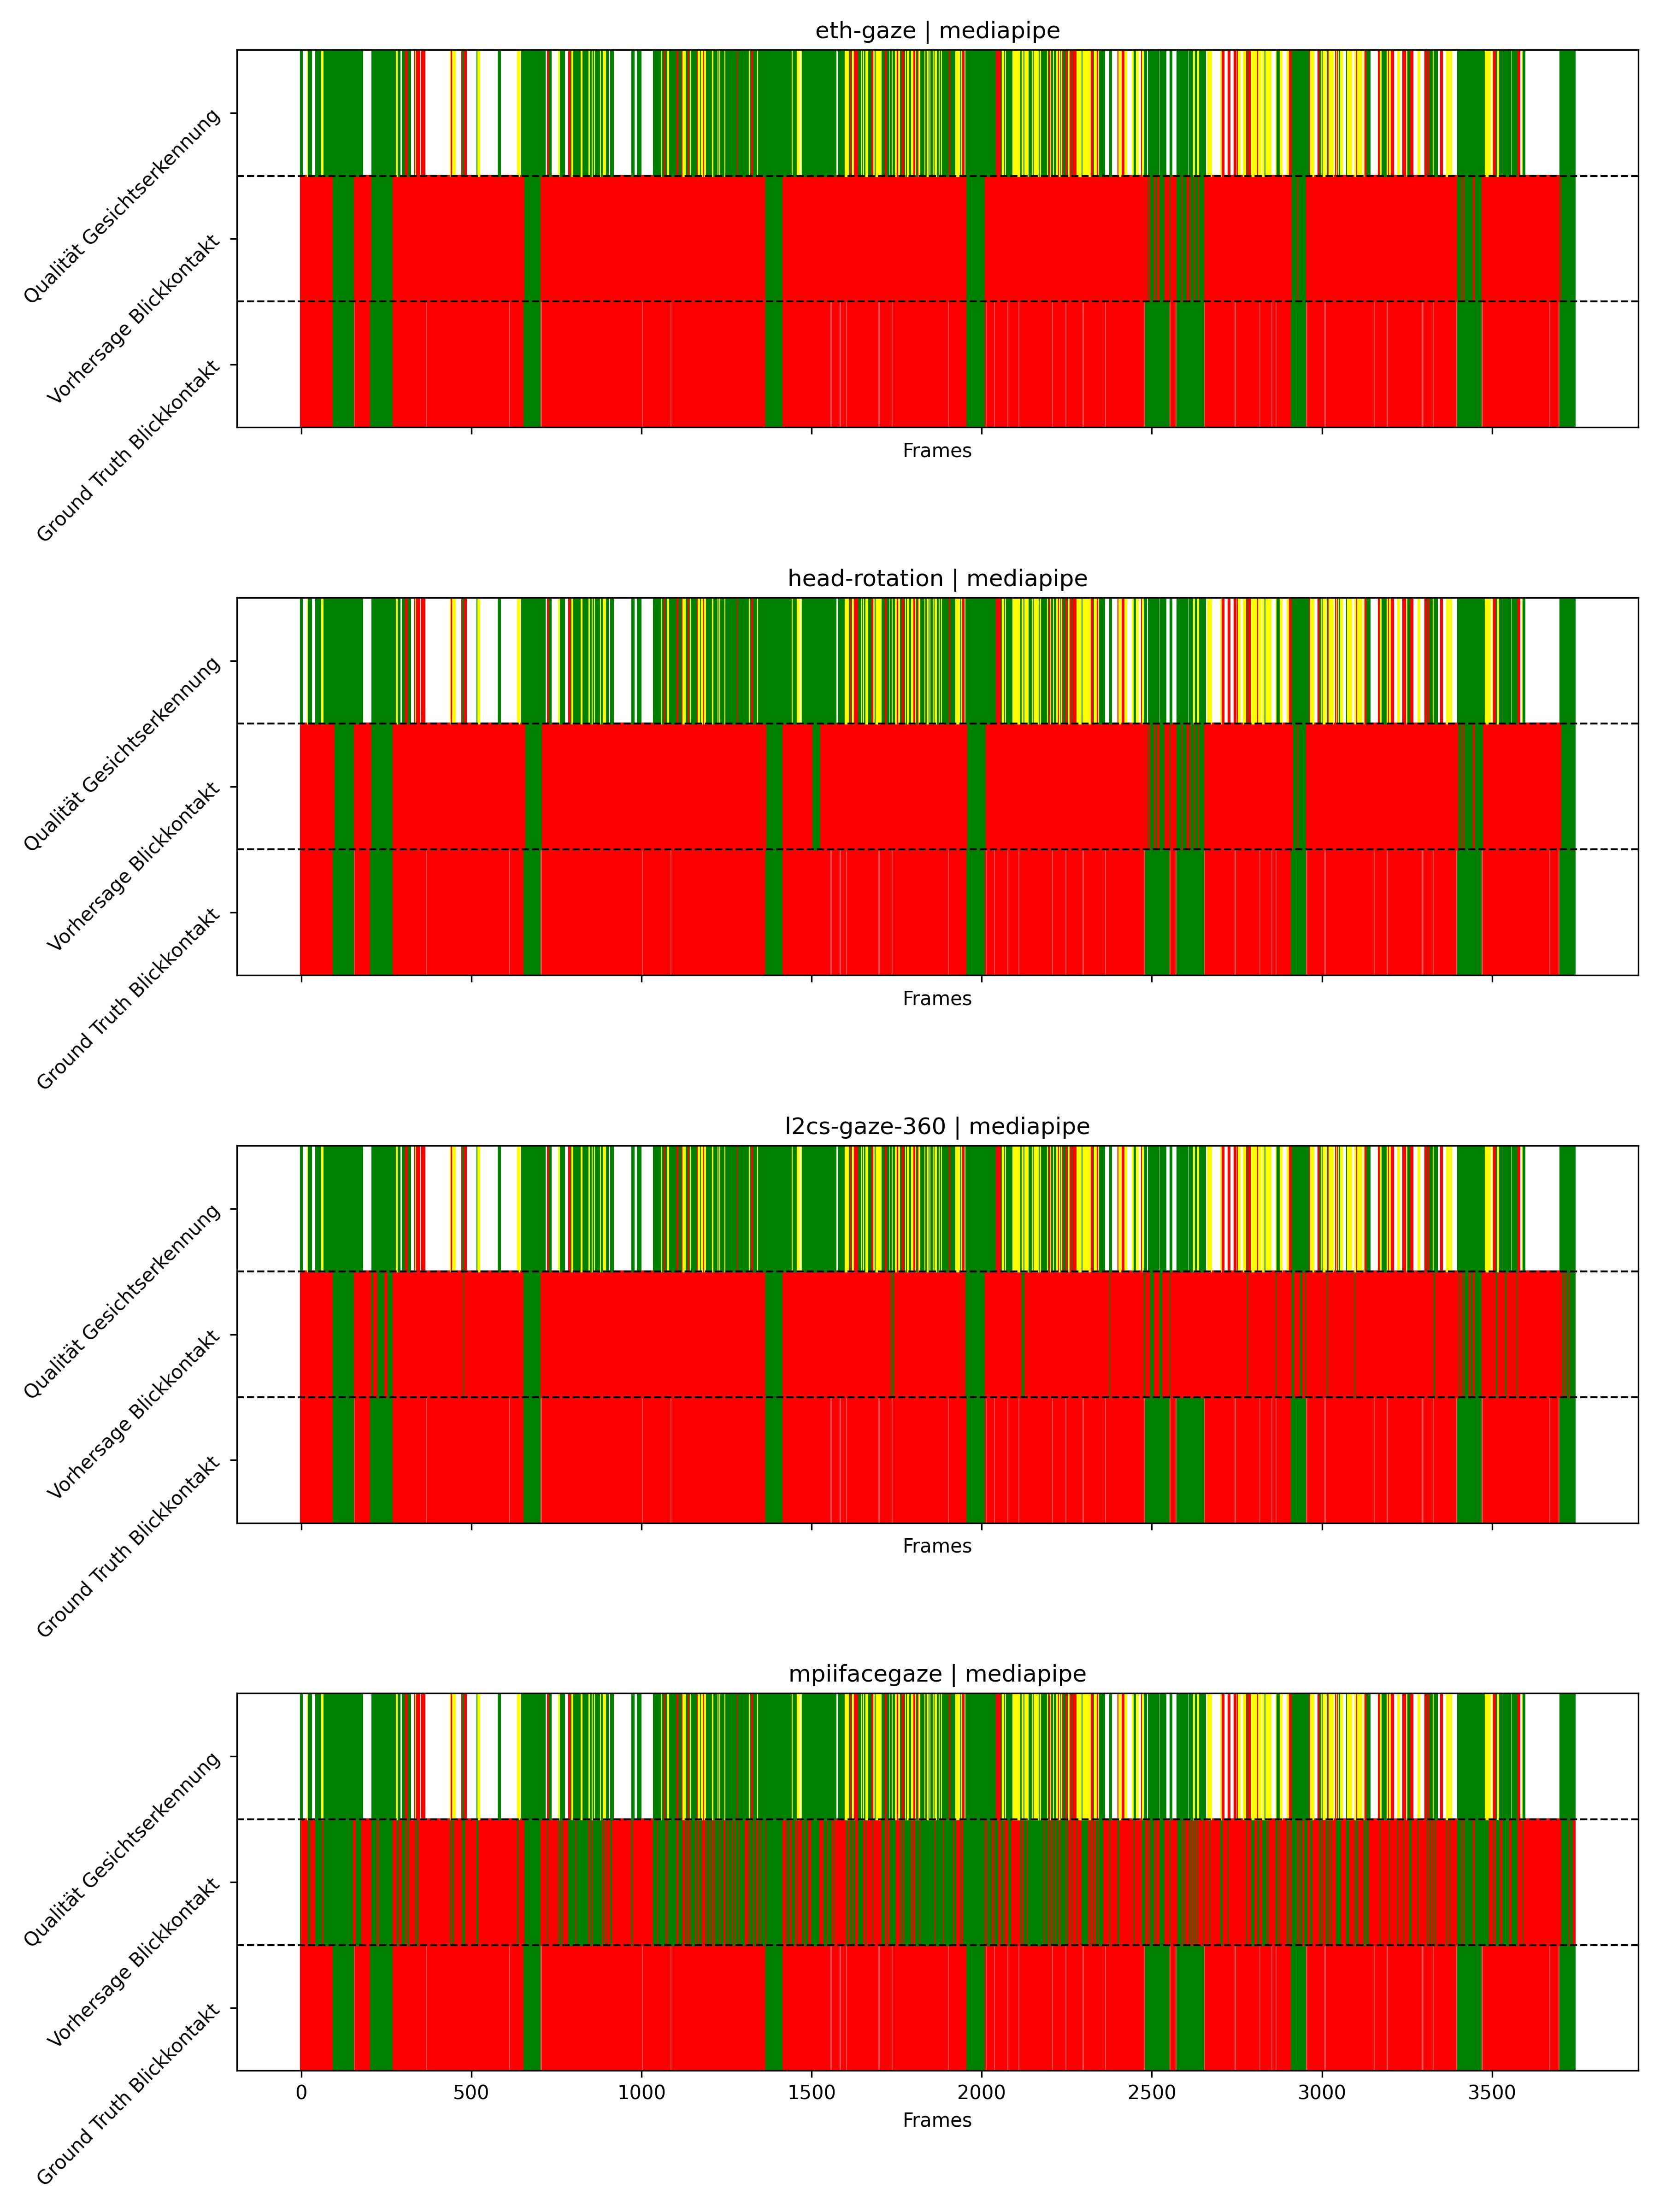
\includegraphics[width=1\linewidth]{appendix/14-mediapipe-overview-gaze.jpg}
\caption{Überblick über die Ground Truth des Blickkontakts, die Vorhersage des Blickkontakts und die Qualität der Gesichtserkennung mit \mediapipe. Die Bedeutung der Farben ist in Abbildung \ref{fig:evaluation:gaze:mpiifacegaze} erklärt.}
\end{figure}

\section{Video 15}
\begin{figure}[H]
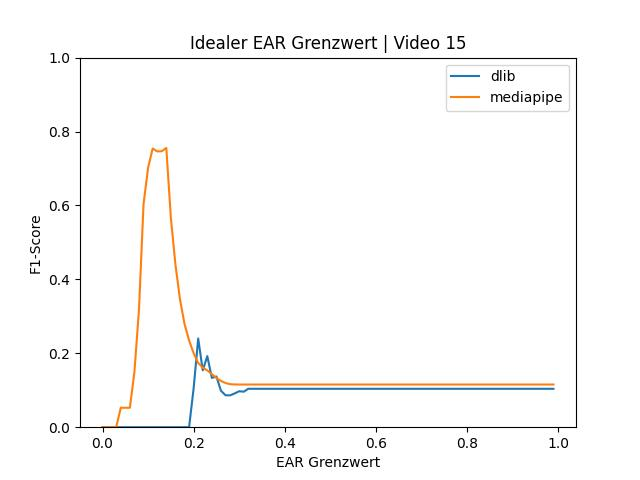
\includegraphics[width=0.7\linewidth]{appendix/15_f1-score-blink.jpg}
\caption{Ergebnisse der Bestimmung des idealen EAR-Grenzwerts für Video 15.}
\end{figure}

\begin{figure}[H]
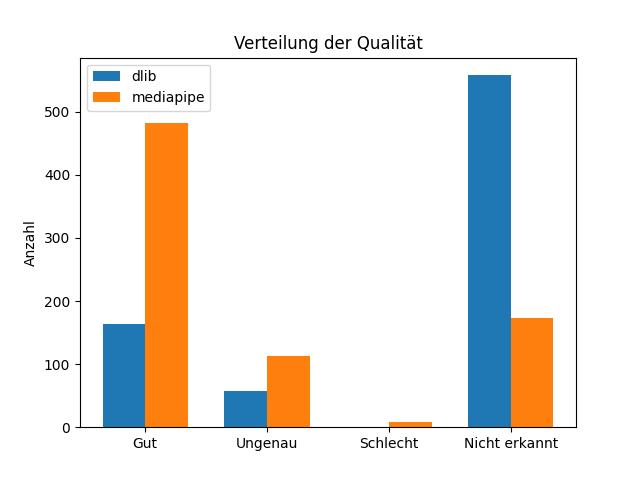
\includegraphics[width=0.7\linewidth]{appendix/15_bar-quality.jpg}
\caption{Aufteilung der Gesichtserkennungsqualität von Video 15.}
\end{figure}

\begin{table}[H]
\centering
\begin{tabular}{l|l|c c |c}
\toprule
\textbf{Gesichtserkennung} & \textbf{Blickrichtung} & \textbf{Seitenlänge} $\hitthresholdsize$ & \textbf{Verschiebung} $\hitthresholdposition$ & \textbf{F1-Score} \\ 
\midrule
\multirow{4}*{dlib}& ETH-XGaze & 0,133 & 0,01 & 0,988  \\ 
& Gaze360 & 0,5 & 0,047 & 0,945 \\ 
& MPIIFaceGaze & 0,102 & -0,027 & 0,893  \\ 
& Kopfrotation & 0,214 & 0,231 & 0,863  \\ 
\hline\multirow{4}*{MediaPipe}& ETH-XGaze & 0,133 & 0,01 & 0,988  \\ 
& Gaze360 & 0,5 & 0,047 & 0,929 \\ 
& MPIIFaceGaze & 0,071 & -0,039 & 0,62  \\ 
& Kopfrotation & 0,133 & 0,194 & 0,961  \\ 
\bottomrule\end{tabular}
\caption{Ergebnis des Hyperparameter-Tunings für die Zone speziell für Video 15.}
\label{tab:appendix:15:local}
\end{table}
\begin{table}[H]
\centering
\begin{tabular}{l|l|c c c c|c c|c}
\toprule
\textbf{Gesichtserkennung} & \textbf{Blickrichtung} & $TP$ & $TN$& $FP$ & $FN$ & \textbf{Precision} & \textbf{Recall} & \textbf{F1-Score} \\ 
\midrule
\multirow{4}*{dlib}& ETH-XGaze & 167 & 606 & 5 & 0 & 0,971 & 1,0 & 0,985 \\ 
& Gaze360 & 155 & 605 & 6 & 12 & 0,963 & 0,928 & 0,945 \\ 
& MPIIFaceGaze & 156 & 584 & 27 & 11 & 0,852 & 0,934 & 0,891 \\ 
& Kopfrotation & 166 & 558 & 53 & 1 & 0,758 & 0,994 & 0,86 \\ 
\hline\multirow{4}*{MediaPipe}& ETH-XGaze & 167 & 606 & 5 & 0 & 0,971 & 1,0 & 0,985 \\ 
& Gaze360 & 143 & 605 & 6 & 24 & 0,96 & 0,856 & 0,905 \\ 
& MPIIFaceGaze & 99 & 396 & 215 & 68 & 0,315 & 0,593 & 0,412 \\ 
& Kopfrotation & 162 & 600 & 11 & 5 & 0,936 & 0,97 & 0,953 \\ 
\bottomrule\end{tabular}
\caption{Zusammensetzung des F1-Scores unter Verwendung der in Kapitel \ref{sec:evaluation:results:gaze:threshold} bestimmten globalen Parameter $\hitthresholdsize$ und $\hitthresholdposition$.}
\label{tab:appendix:15:f1}
\end{table}
\begin{figure}[H]
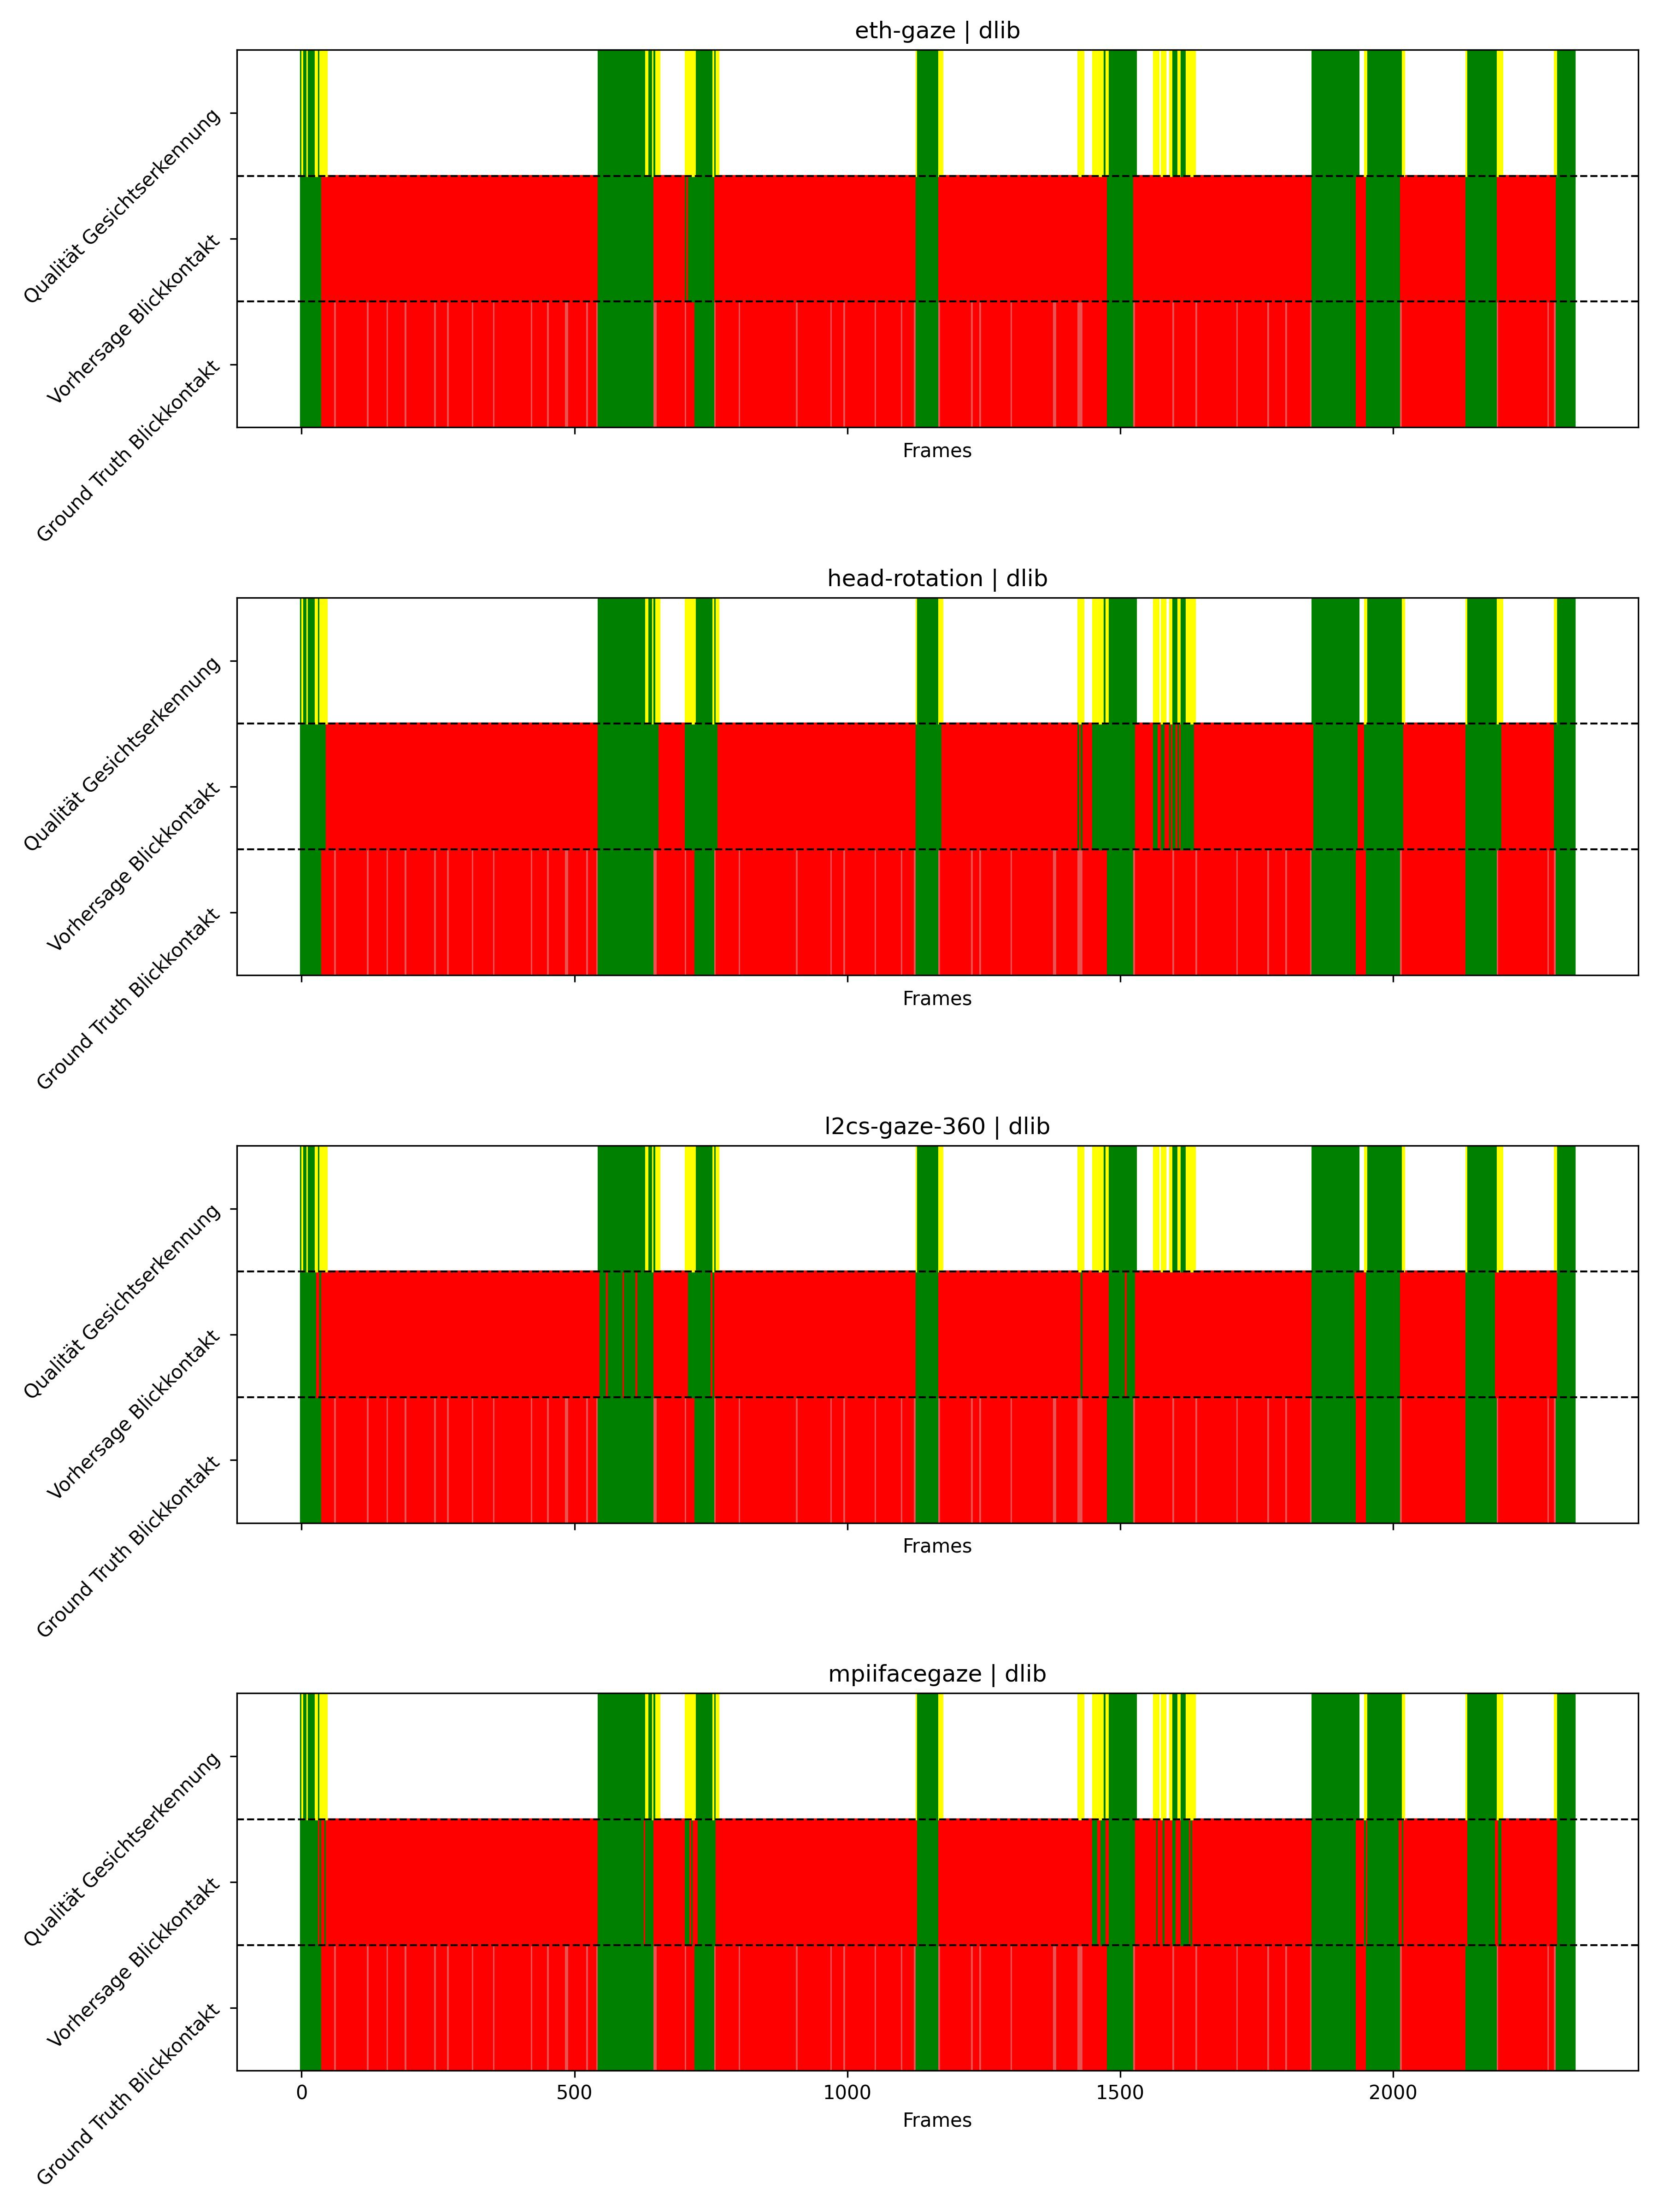
\includegraphics[width=1\linewidth]{appendix/15-dlib-overview-gaze.jpg}
\caption{Überblick über die Ground Truth des Blickkontakts, die Vorhersage des Blickkontakts und die Qualität der Gesichtserkennung mit \dlib. Die Bedeutung der Farben ist in Abbildung \ref{fig:evaluation:gaze:mpiifacegaze} erklärt.  }
\end{figure}

\begin{figure}[H]
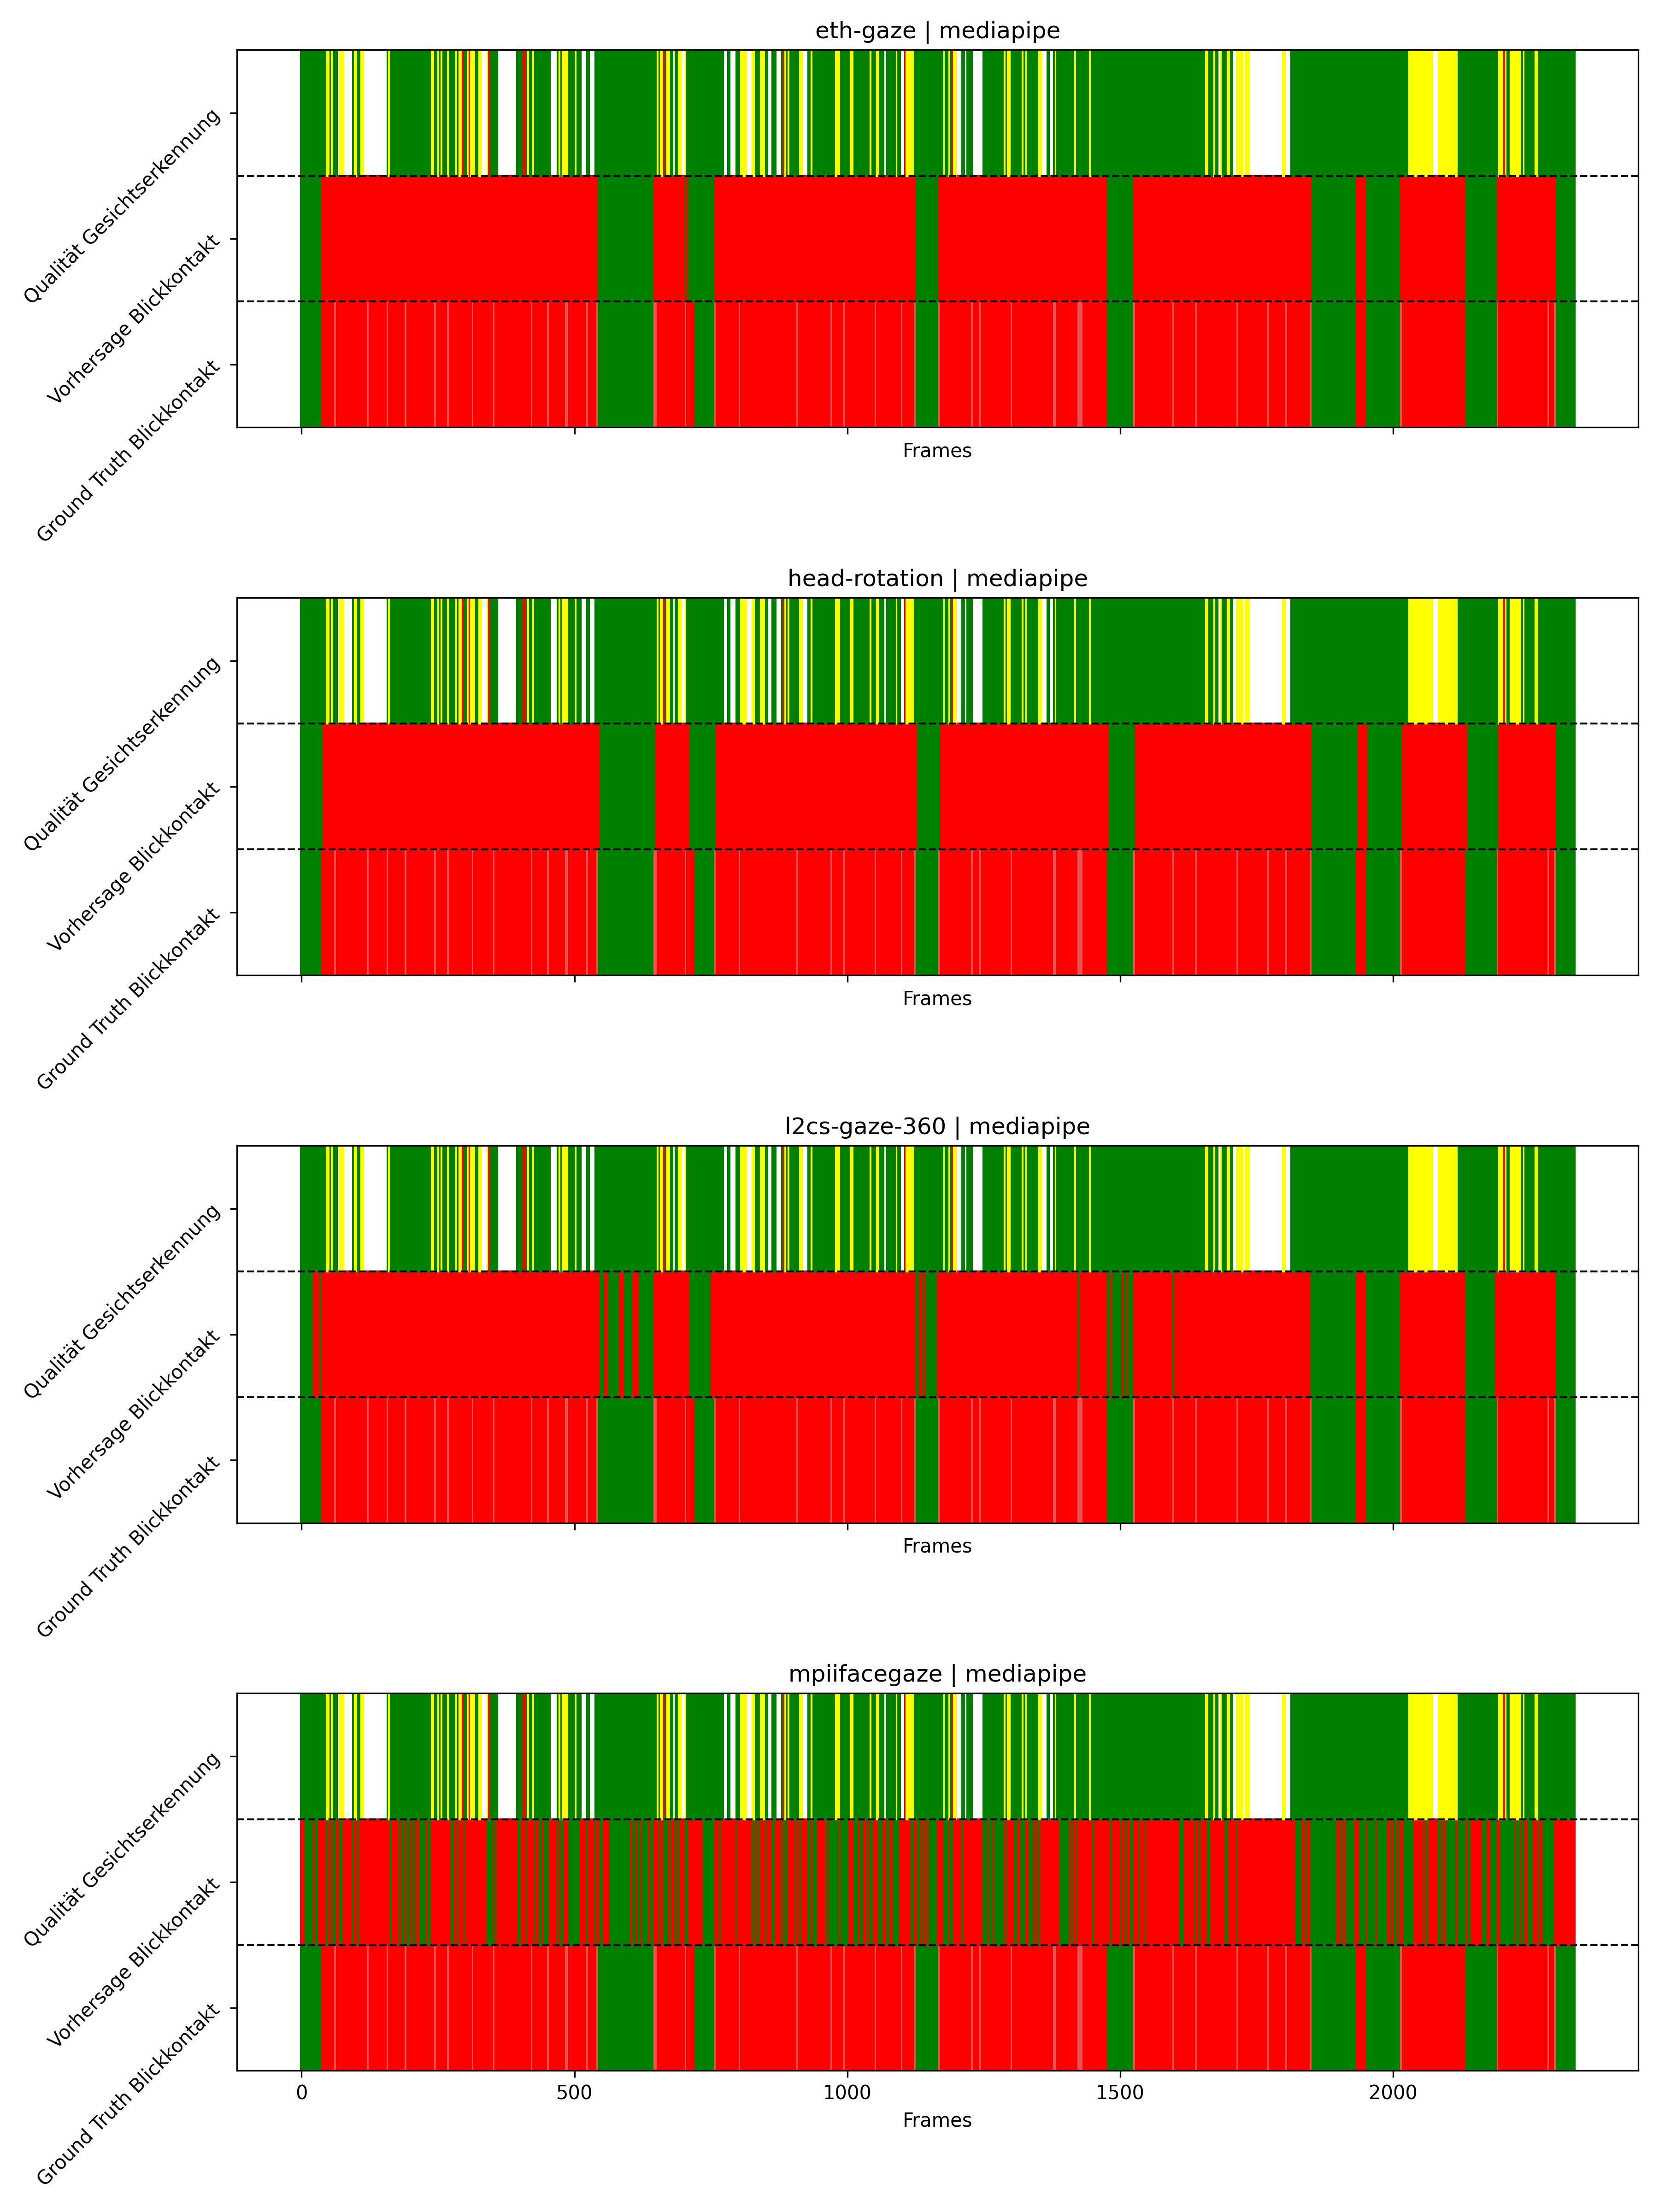
\includegraphics[width=1\linewidth]{appendix/15-mediapipe-overview-gaze.jpg}
\caption{Überblick über die Ground Truth des Blickkontakts, die Vorhersage des Blickkontakts und die Qualität der Gesichtserkennung mit \mediapipe. Die Bedeutung der Farben ist in Abbildung \ref{fig:evaluation:gaze:mpiifacegaze} erklärt.}
\end{figure}

\section{Video 16}
\begin{figure}[H]
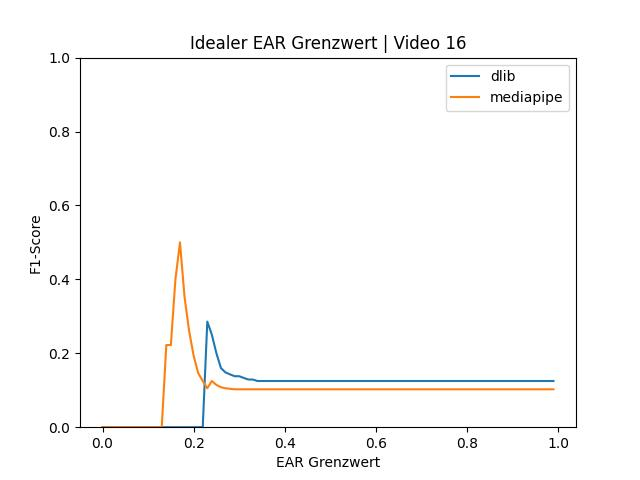
\includegraphics[width=0.7\linewidth]{appendix/16_f1-score-blink.jpg}
\caption{Ergebnisse der Bestimmung des idealen EAR-Grenzwerts für Video 16.}
\end{figure}

\begin{figure}[H]
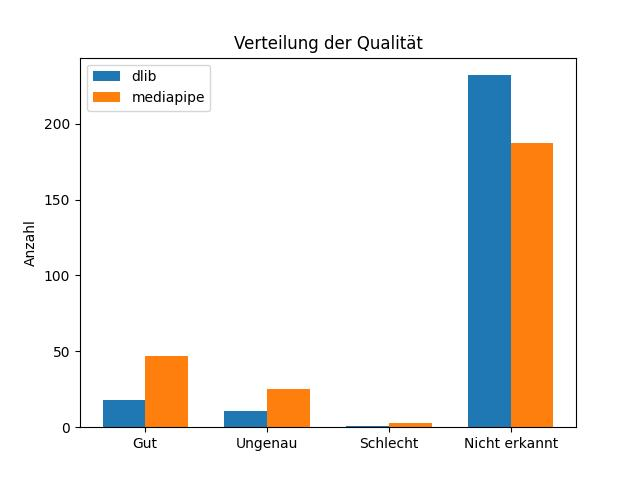
\includegraphics[width=0.7\linewidth]{appendix/16_bar-quality.jpg}
\caption{Aufteilung der Gesichtserkennungsqualität von Video 16.}
\end{figure}

\begin{table}[H]
\centering
\begin{tabular}{l|l|c c |c}
\toprule
\textbf{Gesichtserkennung} & \textbf{Blickrichtung} & \textbf{Seitenlänge} $\hitthresholdsize$ & \textbf{Verschiebung} $\hitthresholdposition$ & \textbf{F1-Score} \\ 
\midrule
\multirow{4}*{dlib}& ETH-XGaze & 0,133 & -0,002 & 1,0  \\ 
& Gaze360 & 0,245 & 0,059 & 0,976 \\ 
& MPIIFaceGaze & 0,071 & -0,014 & 0,864  \\ 
& Kopfrotation & 0,184 & 0,169 & 0,864  \\ 
\hline\multirow{4}*{MediaPipe}& ETH-XGaze & 0,112 & -0,014 & 1,0  \\ 
& Gaze360 & 0,347 & 0,059 & 0,952 \\ 
& MPIIFaceGaze & 0,102 & 0,047 & 0,507  \\ 
& Kopfrotation & 0,276 & 0,194 & 0,974  \\ 
\bottomrule\end{tabular}
\caption{Ergebnis des Hyperparameter-Tunings für die Zone speziell für Video 16.}
\label{tab:appendix:16:local}
\end{table}
\begin{table}[H]
\centering
\begin{tabular}{l|l|c c c c|c c|c}
\toprule
\textbf{Gesichtserkennung} & \textbf{Blickrichtung} & $TP$ & $TN$& $FP$ & $FN$ & \textbf{Precision} & \textbf{Recall} & \textbf{F1-Score} \\ 
\midrule
\multirow{4}*{dlib}& ETH-XGaze & 20 & 240 & 1 & 0 & 0,952 & 1,0 & 0,976 \\ 
& Gaze360 & 19 & 238 & 3 & 1 & 0,864 & 0,95 & 0,905 \\ 
& MPIIFaceGaze & 18 & 236 & 5 & 2 & 0,783 & 0,9 & 0,837 \\ 
& Kopfrotation & 20 & 234 & 7 & 0 & 0,741 & 1,0 & 0,851 \\ 
\hline\multirow{4}*{MediaPipe}& ETH-XGaze & 20 & 240 & 2 & 0 & 0,909 & 1,0 & 0,952 \\ 
& Gaze360 & 19 & 240 & 2 & 1 & 0,905 & 0,95 & 0,927 \\ 
& MPIIFaceGaze & 16 & 209 & 33 & 4 & 0,327 & 0,8 & 0,464 \\ 
& Kopfrotation & 20 & 240 & 2 & 0 & 0,909 & 1,0 & 0,952 \\ 
\bottomrule\end{tabular}
\caption{Zusammensetzung des F1-Scores unter Verwendung der in Kapitel \ref{sec:evaluation:results:gaze:threshold} bestimmten globalen Parameter $\hitthresholdsize$ und $\hitthresholdposition$.}
\label{tab:appendix:16:f1}
\end{table}
\begin{figure}[H]
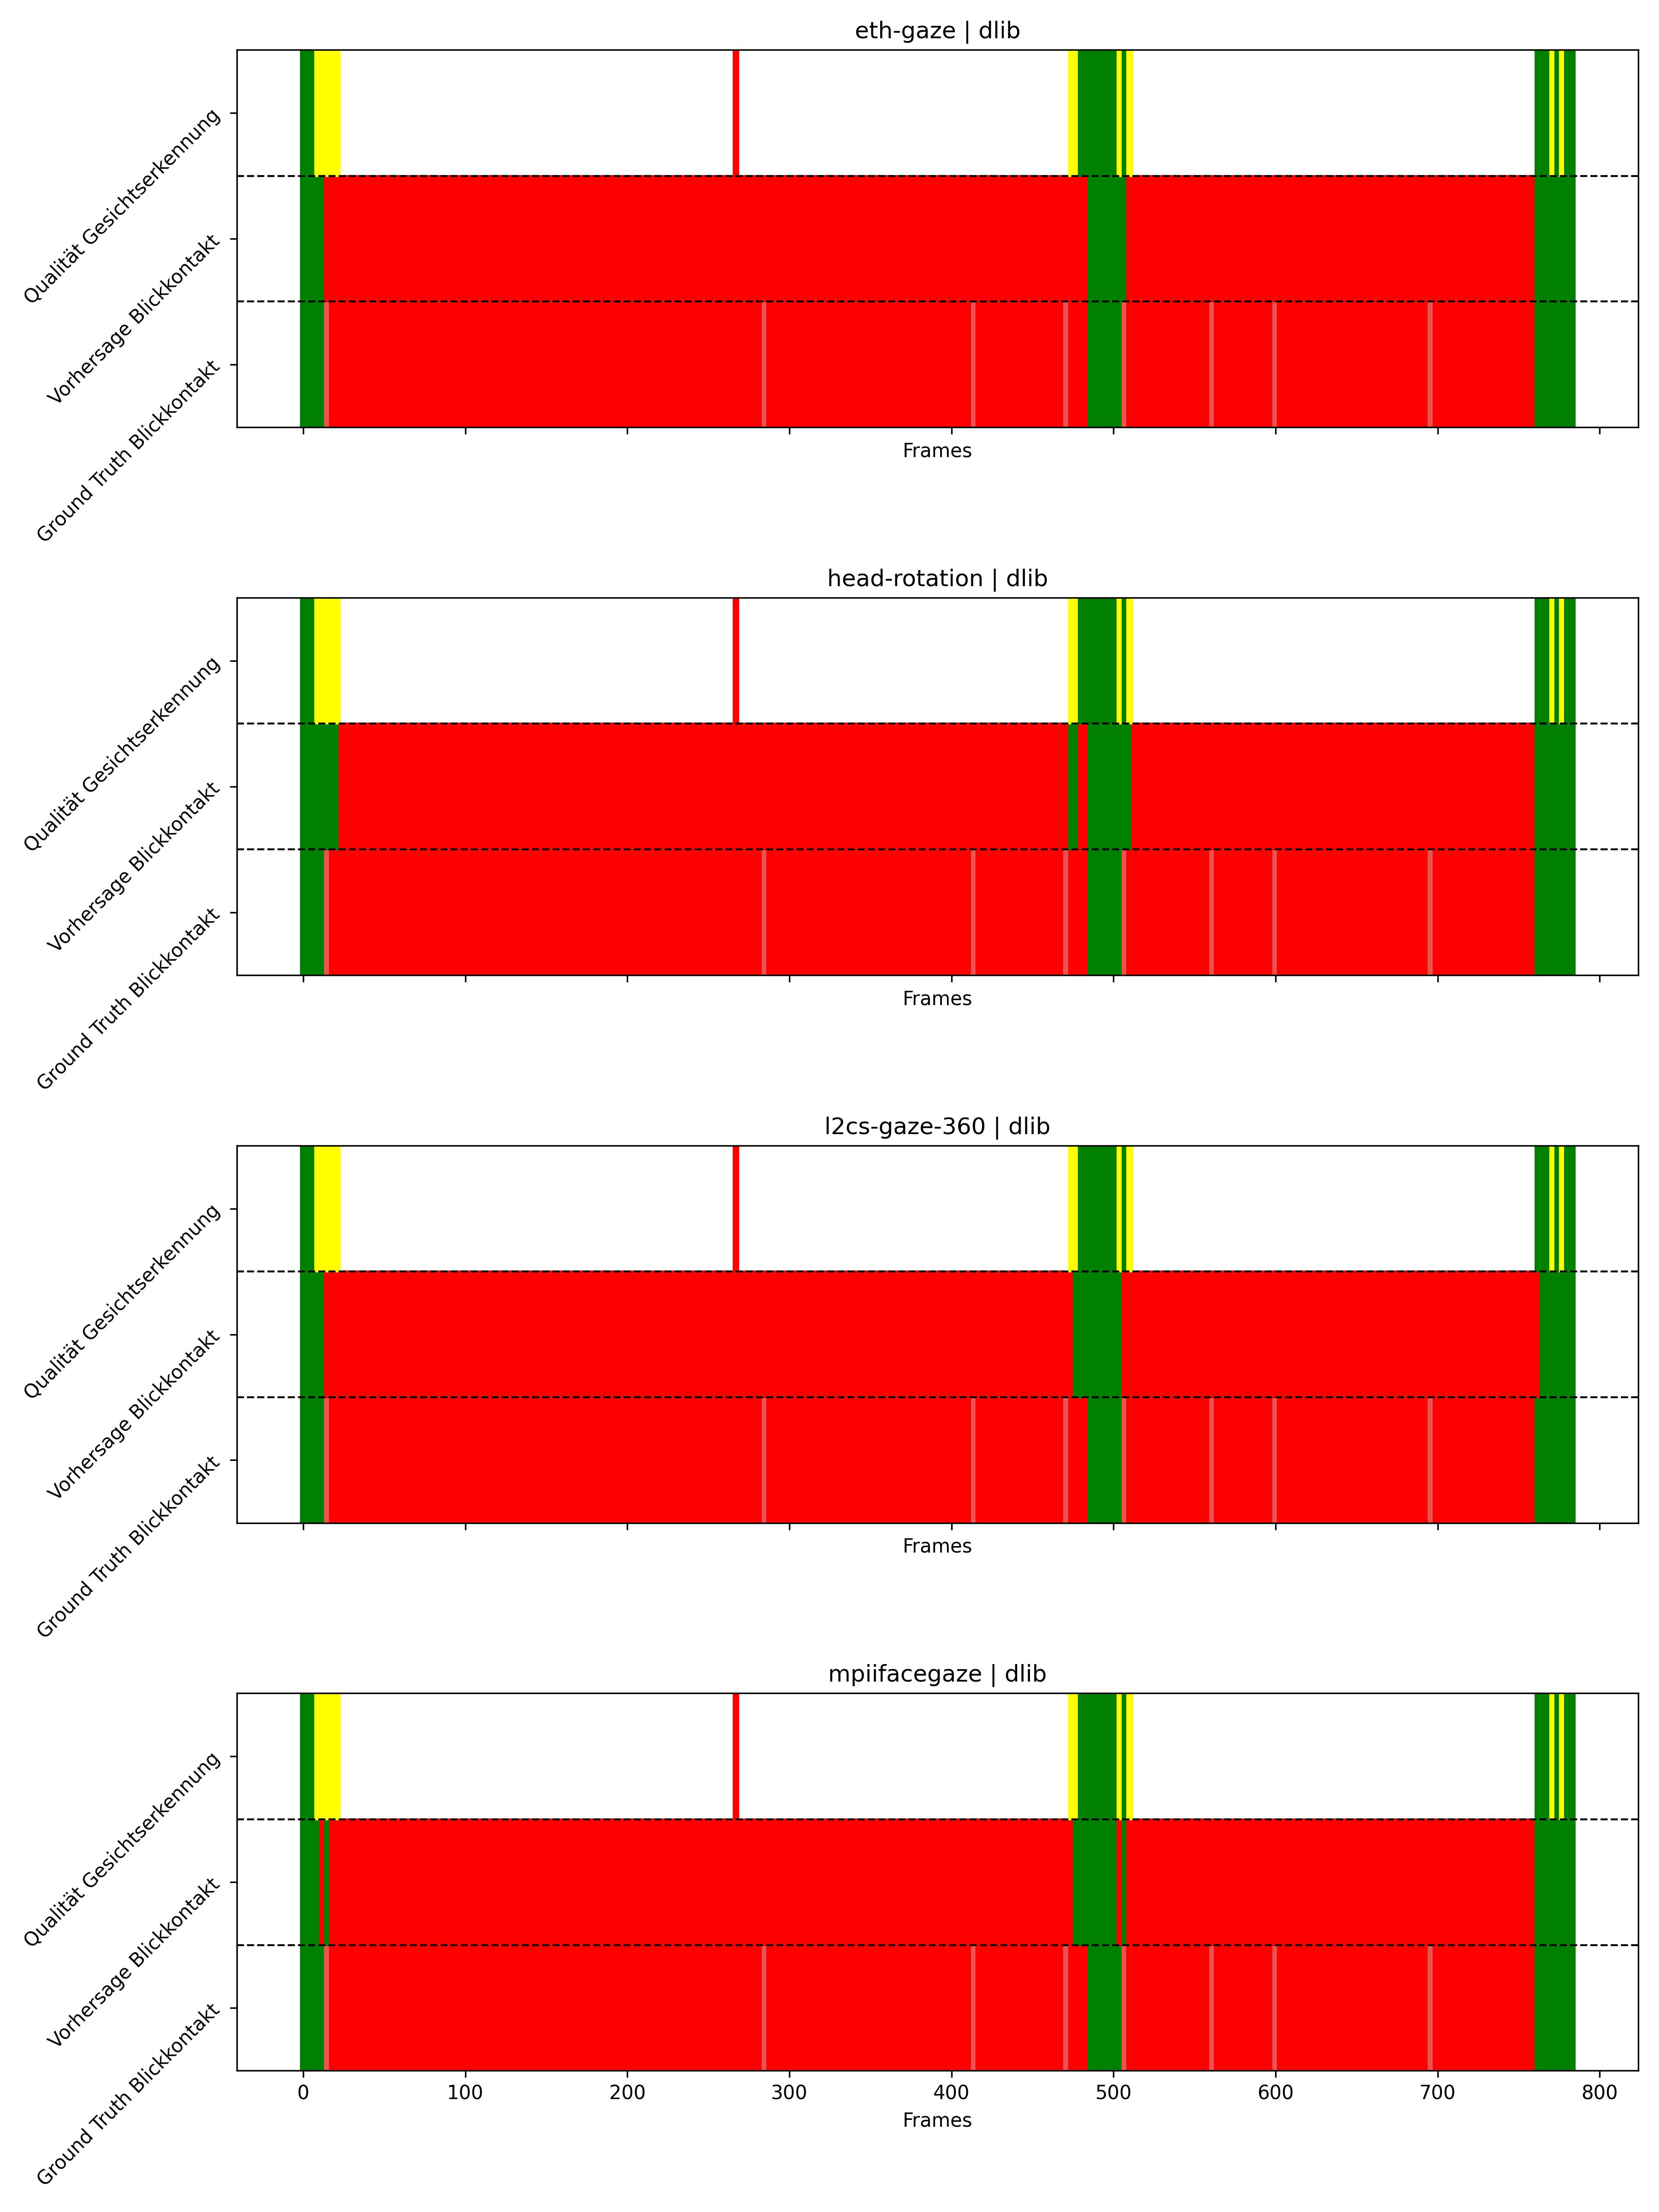
\includegraphics[width=1\linewidth]{appendix/16-dlib-overview-gaze.jpg}
\caption{Überblick über die Ground Truth des Blickkontakts, die Vorhersage des Blickkontakts und die Qualität der Gesichtserkennung mit \dlib. Die Bedeutung der Farben ist in Abbildung \ref{fig:evaluation:gaze:mpiifacegaze} erklärt.  }
\end{figure}

\begin{figure}[H]
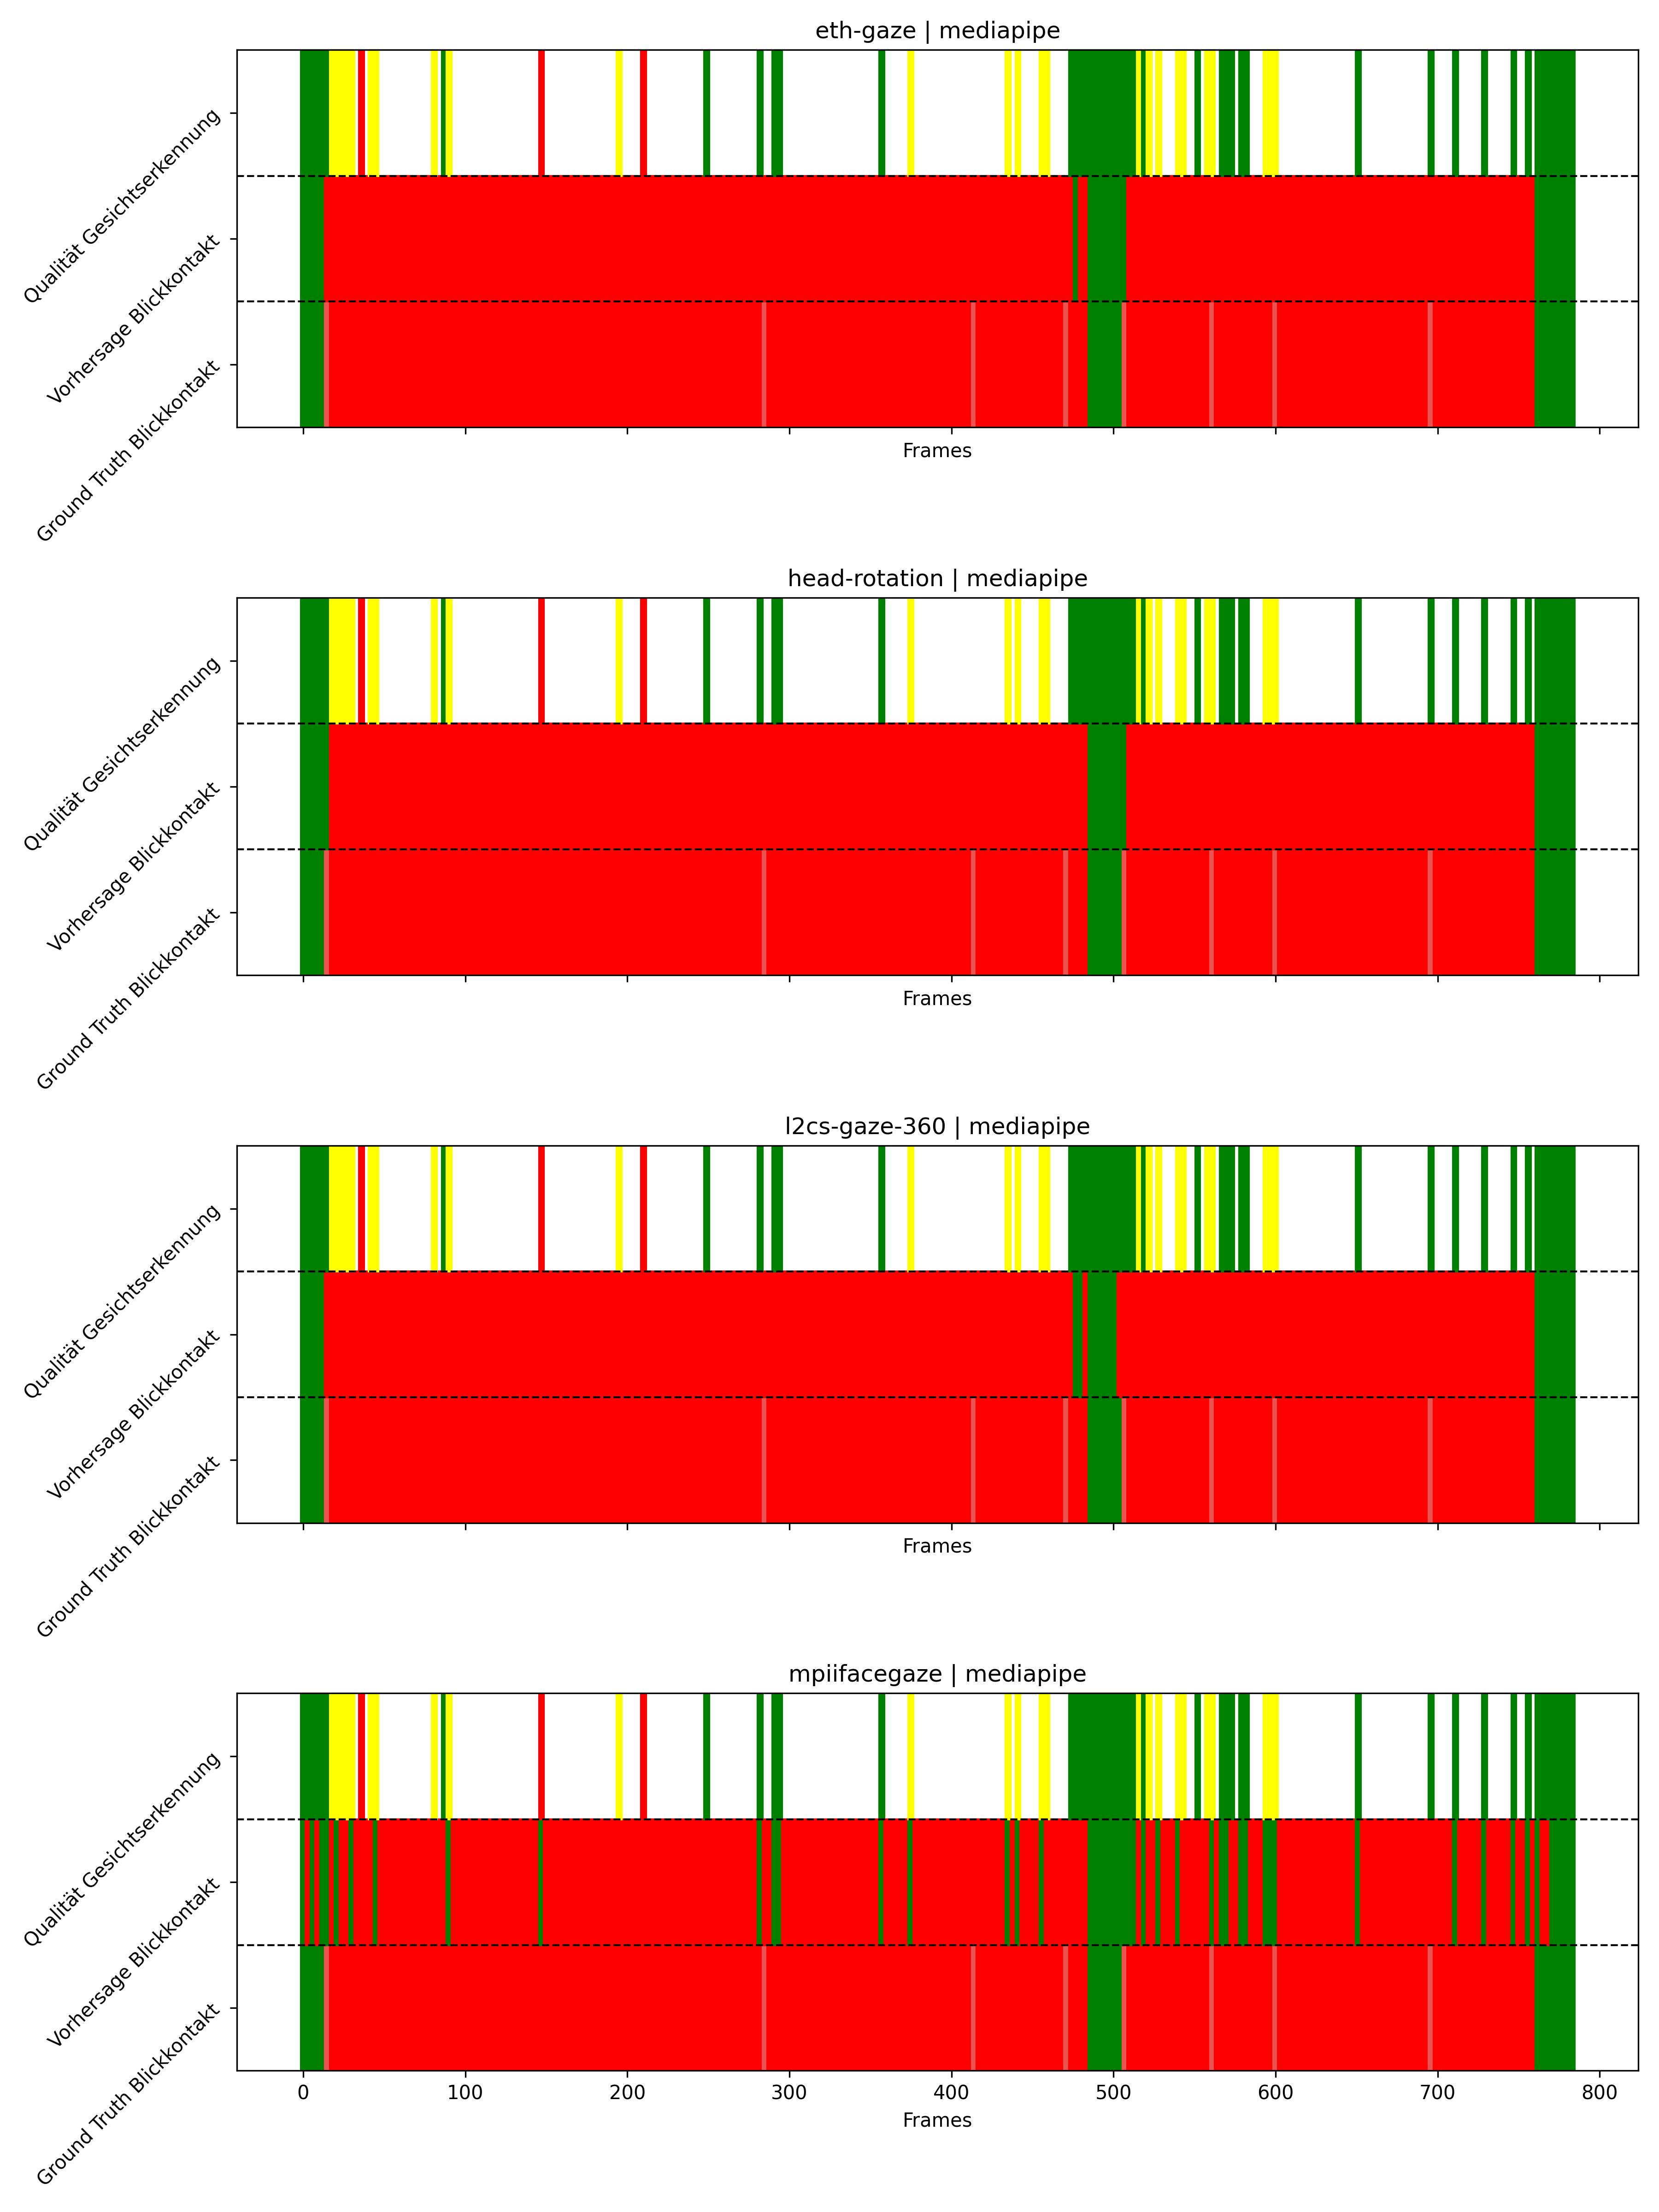
\includegraphics[width=1\linewidth]{appendix/16-mediapipe-overview-gaze.jpg}
\caption{Überblick über die Ground Truth des Blickkontakts, die Vorhersage des Blickkontakts und die Qualität der Gesichtserkennung mit \mediapipe. Die Bedeutung der Farben ist in Abbildung \ref{fig:evaluation:gaze:mpiifacegaze} erklärt.}
\end{figure}

\section{Video 17}
\begin{figure}[H]
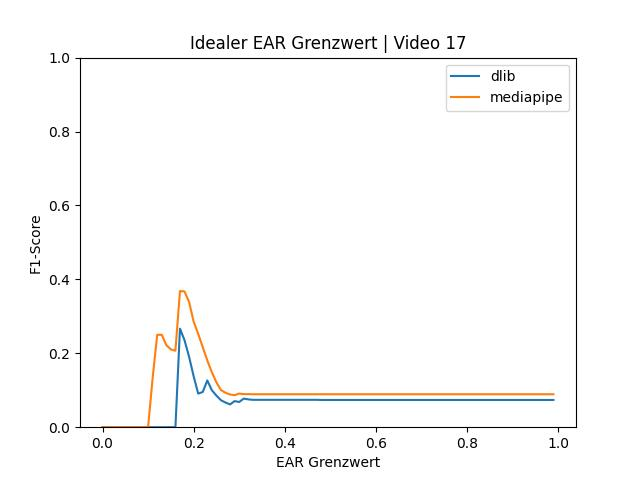
\includegraphics[width=0.7\linewidth]{appendix/17_f1-score-blink.jpg}
\caption{Ergebnisse der Bestimmung des idealen EAR-Grenzwerts für Video 17.}
\end{figure}

\begin{figure}[H]
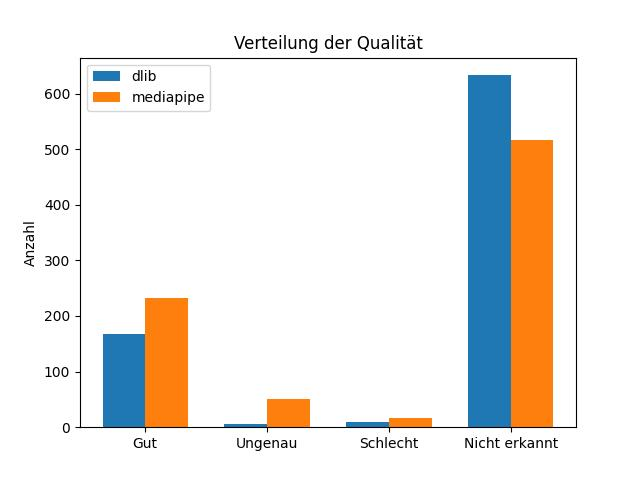
\includegraphics[width=0.7\linewidth]{appendix/17_bar-quality.jpg}
\caption{Aufteilung der Gesichtserkennungsqualität von Video 17.}
\end{figure}

\begin{table}[H]
\centering
\begin{tabular}{l|l|c c |c}
\toprule
\textbf{Gesichtserkennung} & \textbf{Blickrichtung} & \textbf{Seitenlänge} $\hitthresholdsize$ & \textbf{Verschiebung} $\hitthresholdposition$ & \textbf{F1-Score} \\ 
\midrule
\multirow{4}*{dlib}& ETH-XGaze & 0,173 & 0,047 & 0,869  \\ 
& Gaze360 & 0,48 & 0,427 & 0,838 \\ 
& MPIIFaceGaze & 0,051 & -0,027 & 0,881  \\ 
& Kopfrotation & 0,204 & 0,243 & 0,865  \\ 
\hline\multirow{4}*{MediaPipe}& ETH-XGaze & 0,153 & -0,002 & 0,918  \\ 
& Gaze360 & 0,49 & 0,451 & 0,804 \\ 
& MPIIFaceGaze & 0,051 & -0,039 & 0,838  \\ 
& Kopfrotation & 0,245 & 0,28 & 0,911  \\ 
\bottomrule\end{tabular}
\caption{Ergebnis des Hyperparameter-Tunings für die Zone speziell für Video 17.}
\label{tab:appendix:17:local}
\end{table}
\begin{table}[H]
\centering
\begin{tabular}{l|l|c c c c|c c|c}
\toprule
\textbf{Gesichtserkennung} & \textbf{Blickrichtung} & $TP$ & $TN$& $FP$ & $FN$ & \textbf{Precision} & \textbf{Recall} & \textbf{F1-Score} \\ 
\midrule
\multirow{4}*{dlib}& ETH-XGaze & 142 & 619 & 28 & 25 & 0,835 & 0,85 & 0,843 \\ 
& Gaze360 & 116 & 615 & 32 & 51 & 0,784 & 0,695 & 0,737 \\ 
& MPIIFaceGaze & 143 & 614 & 33 & 24 & 0,812 & 0,856 & 0,834 \\ 
& Kopfrotation & 134 & 616 & 31 & 33 & 0,812 & 0,802 & 0,807 \\ 
\hline\multirow{4}*{MediaPipe}& ETH-XGaze & 164 & 615 & 34 & 3 & 0,828 & 0,982 & 0,899 \\ 
& Gaze360 & 94 & 593 & 56 & 73 & 0,627 & 0,563 & 0,593 \\ 
& MPIIFaceGaze & 147 & 595 & 54 & 20 & 0,731 & 0,88 & 0,799 \\ 
& Kopfrotation & 136 & 618 & 31 & 31 & 0,814 & 0,814 & 0,814 \\ 
\bottomrule\end{tabular}
\caption{Zusammensetzung des F1-Scores unter Verwendung der in Kapitel \ref{sec:evaluation:results:gaze:threshold} bestimmten globalen Parameter $\hitthresholdsize$ und $\hitthresholdposition$.}
\label{tab:appendix:17:f1}
\end{table}
\begin{figure}[H]
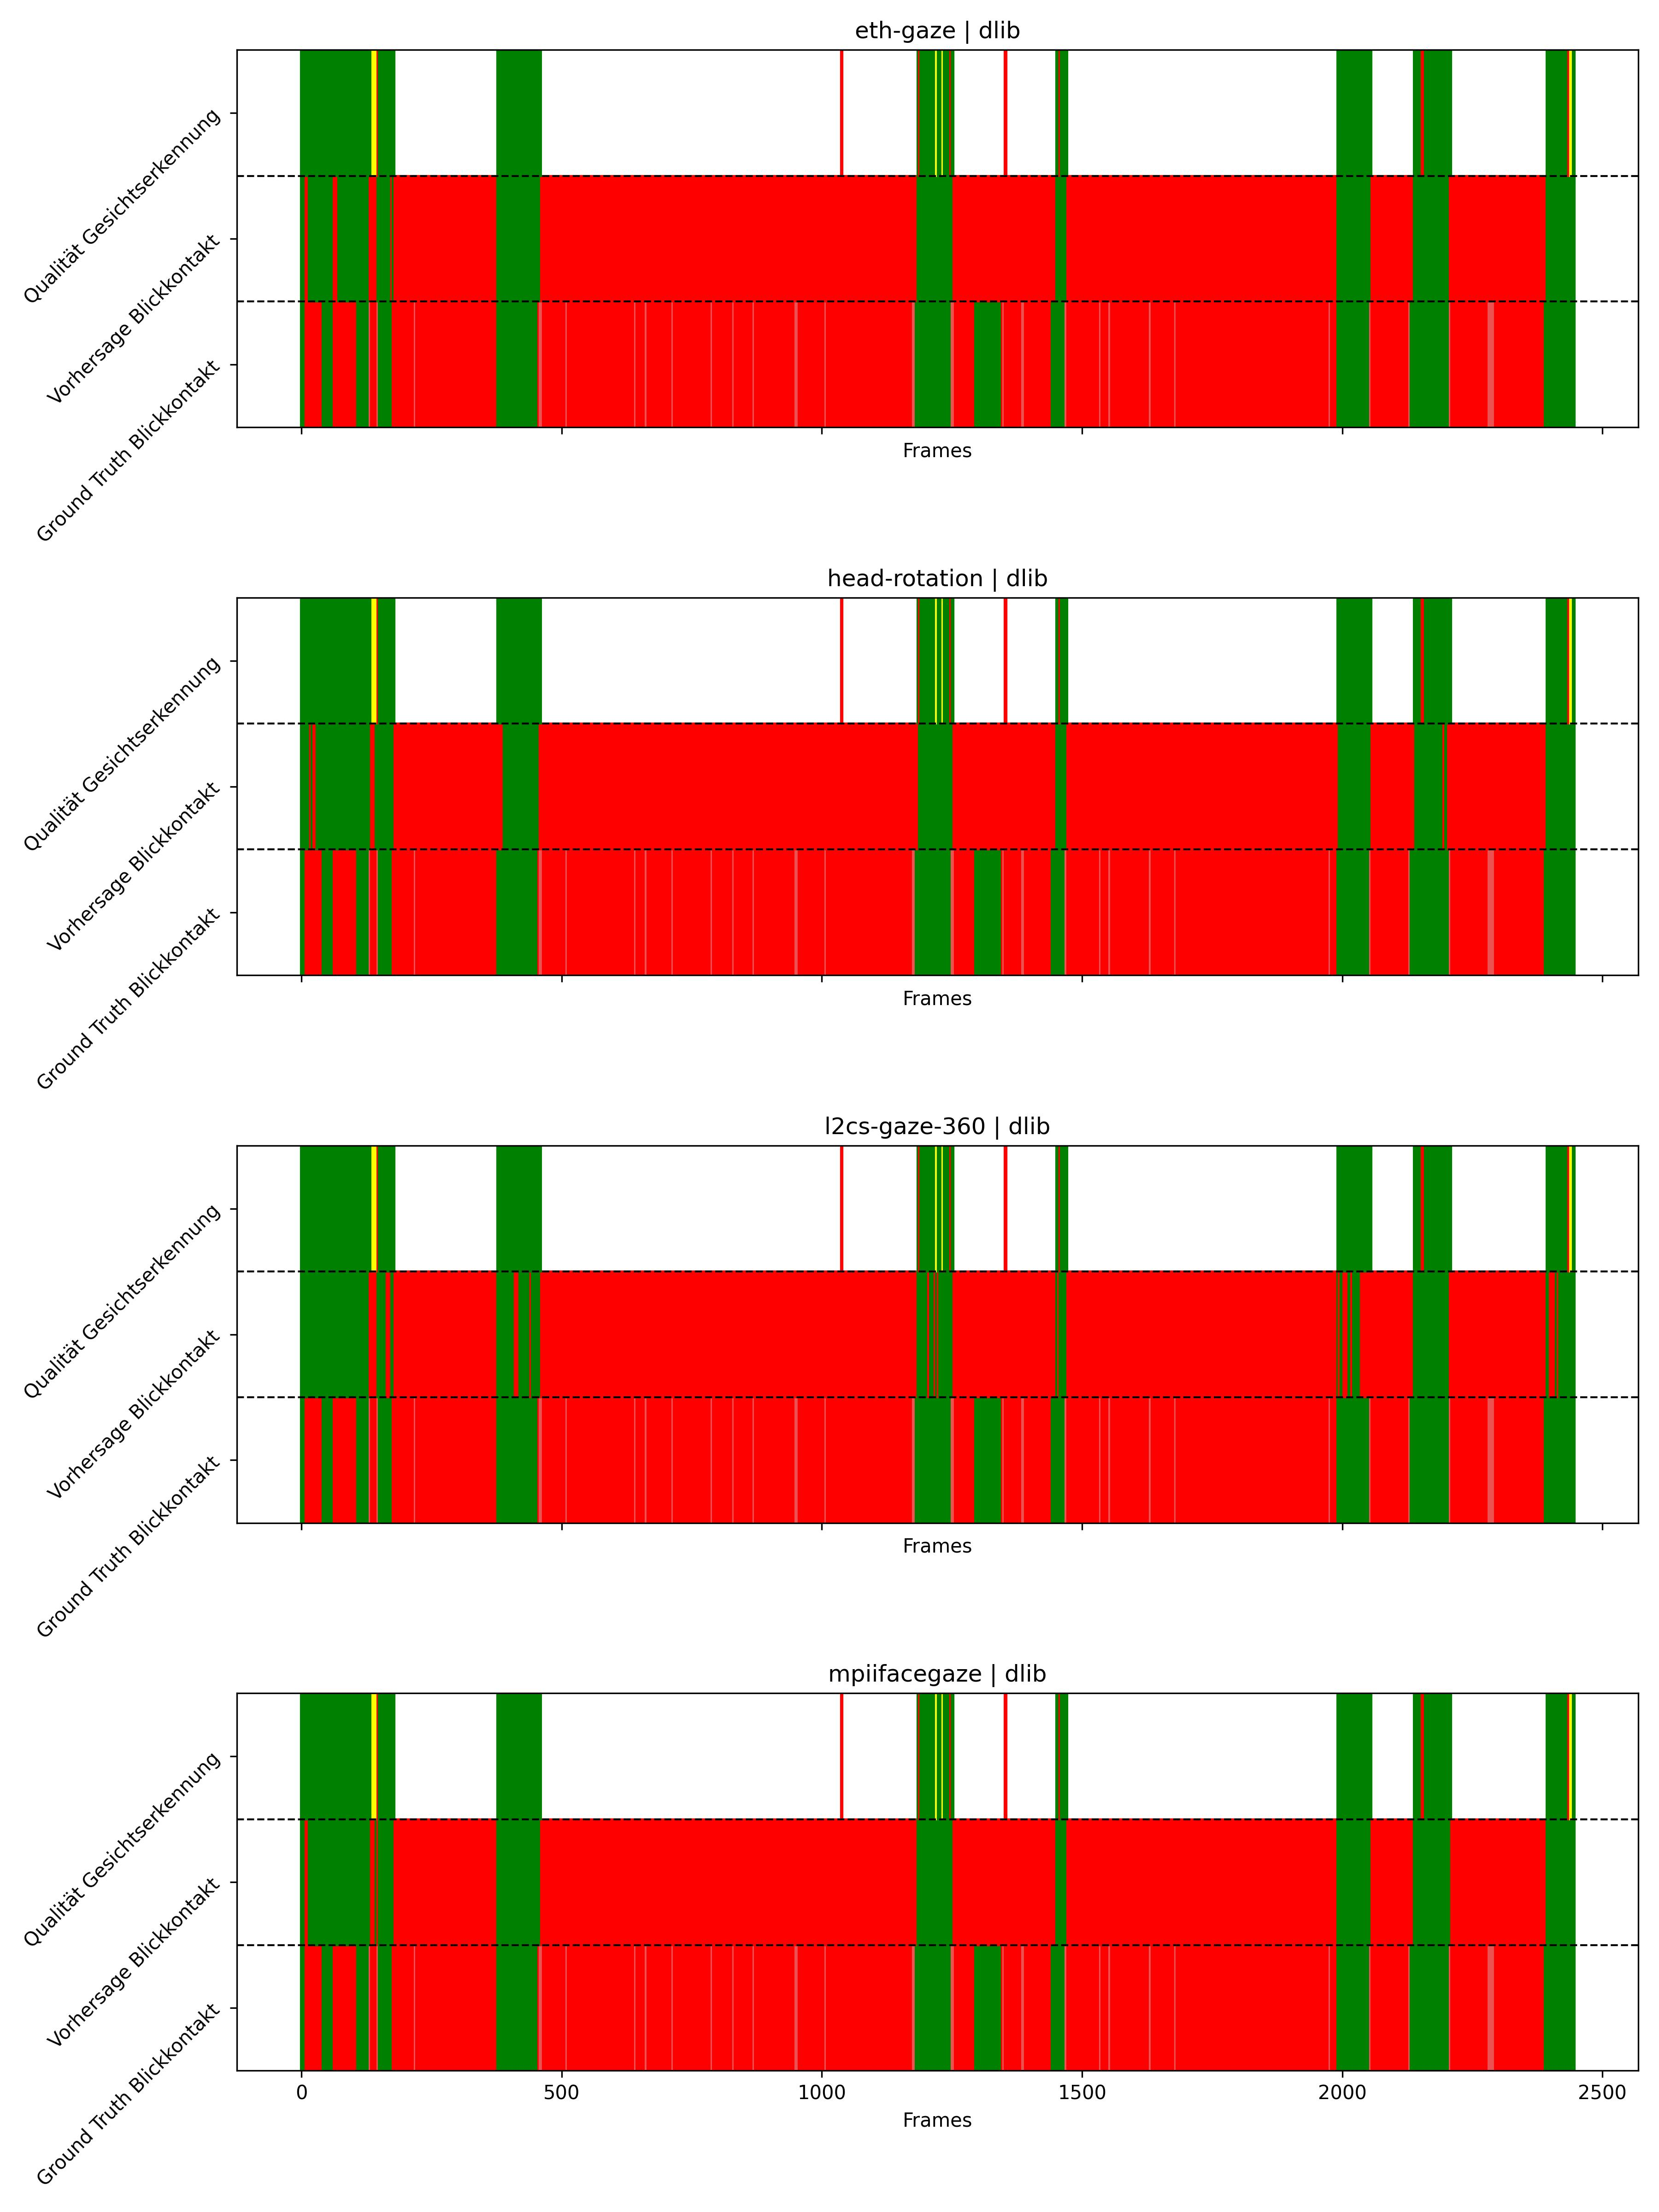
\includegraphics[width=1\linewidth]{appendix/17-dlib-overview-gaze.jpg}
\caption{Überblick über die Ground Truth des Blickkontakts, die Vorhersage des Blickkontakts und die Qualität der Gesichtserkennung mit \dlib. Die Bedeutung der Farben ist in Abbildung \ref{fig:evaluation:gaze:mpiifacegaze} erklärt.  }
\end{figure}

\begin{figure}[H]
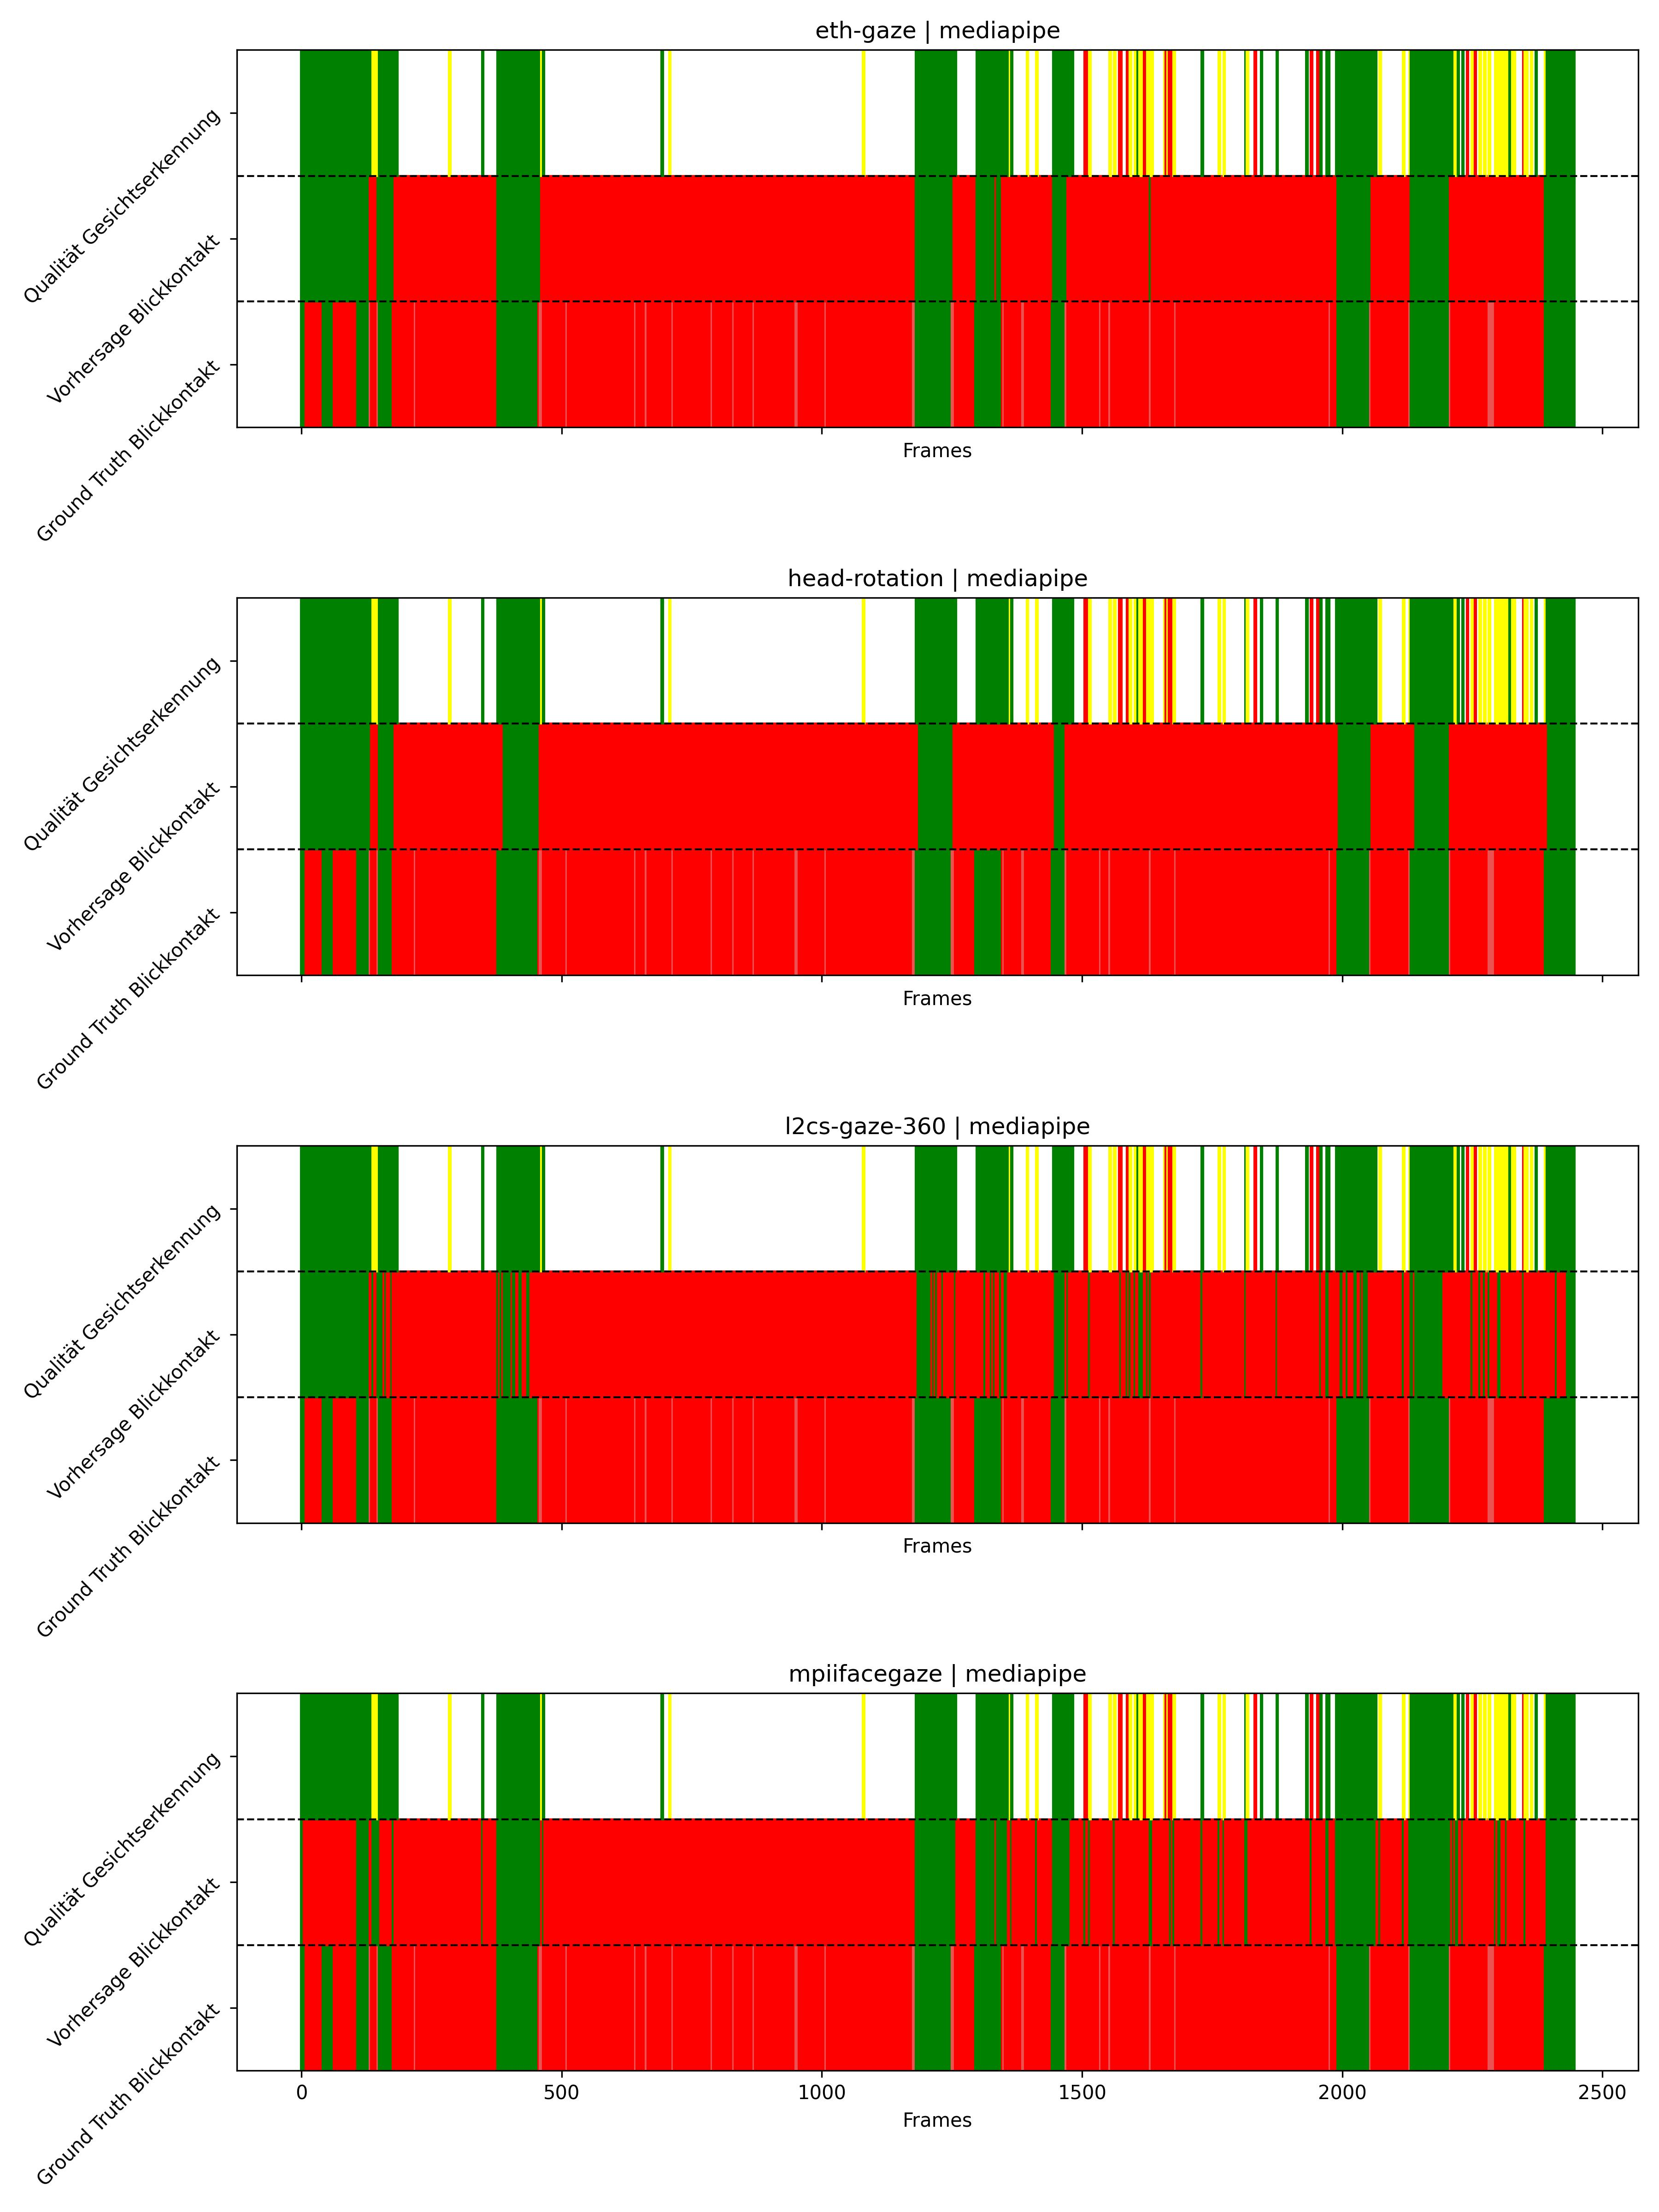
\includegraphics[width=1\linewidth]{appendix/17-mediapipe-overview-gaze.jpg}
\caption{Überblick über die Ground Truth des Blickkontakts, die Vorhersage des Blickkontakts und die Qualität der Gesichtserkennung mit \mediapipe. Die Bedeutung der Farben ist in Abbildung \ref{fig:evaluation:gaze:mpiifacegaze} erklärt.}
\end{figure}

\section{Video 18}
\begin{figure}[H]
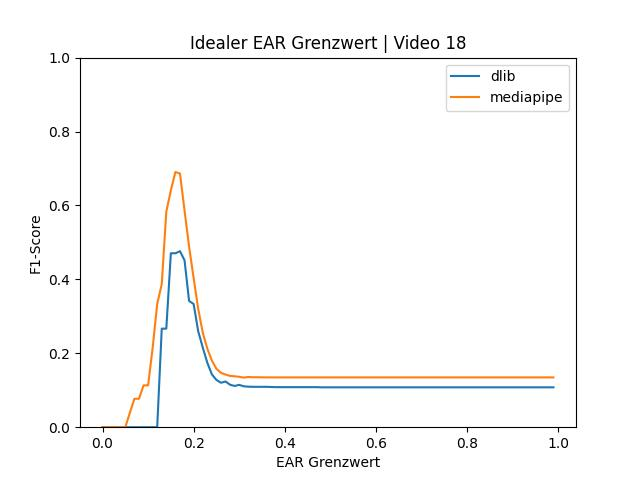
\includegraphics[width=0.7\linewidth]{appendix/18_f1-score-blink.jpg}
\caption{Ergebnisse der Bestimmung des idealen EAR-Grenzwerts für Video 18.}
\end{figure}

\begin{figure}[H]
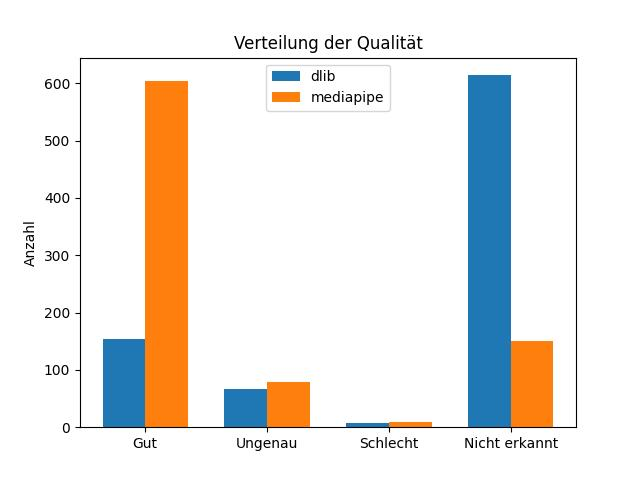
\includegraphics[width=0.7\linewidth]{appendix/18_bar-quality.jpg}
\caption{Aufteilung der Gesichtserkennungsqualität von Video 18.}
\end{figure}

\begin{table}[H]
\centering
\begin{tabular}{l|l|c c |c}
\toprule
\textbf{Gesichtserkennung} & \textbf{Blickrichtung} & \textbf{Seitenlänge} $\hitthresholdsize$ & \textbf{Verschiebung} $\hitthresholdposition$ & \textbf{F1-Score} \\ 
\midrule
\multirow{4}*{dlib}& ETH-XGaze & 0,143 & 0,01 & 0,936  \\ 
& Gaze360 & 0,48 & 0,059 & 0,895 \\ 
& MPIIFaceGaze & 0,071 & 0,022 & 0,615  \\ 
& Kopfrotation & 0,143 & 0,231 & 0,726  \\ 
\hline\multirow{4}*{MediaPipe}& ETH-XGaze & 0,122 & -0,002 & 0,952  \\ 
& Gaze360 & 0,418 & 0,047 & 0,88 \\ 
& MPIIFaceGaze & 0,051 & -0,002 & 0,354  \\ 
& Kopfrotation & 0,133 & 0,231 & 0,921  \\ 
\bottomrule\end{tabular}
\caption{Ergebnis des Hyperparameter-Tunings für die Zone speziell für Video 18.}
\label{tab:appendix:18:local}
\end{table}
\begin{table}[H]
\centering
\begin{tabular}{l|l|c c c c|c c|c}
\toprule
\textbf{Gesichtserkennung} & \textbf{Blickrichtung} & $TP$ & $TN$& $FP$ & $FN$ & \textbf{Precision} & \textbf{Recall} & \textbf{F1-Score} \\ 
\midrule
\multirow{4}*{dlib}& ETH-XGaze & 89 & 729 & 12 & 7 & 0,881 & 0,927 & 0,904 \\ 
& Gaze360 & 82 & 730 & 11 & 14 & 0,882 & 0,854 & 0,868 \\ 
& MPIIFaceGaze & 81 & 635 & 106 & 15 & 0,433 & 0,844 & 0,572 \\ 
& Kopfrotation & 72 & 692 & 49 & 24 & 0,595 & 0,75 & 0,664 \\ 
\hline\multirow{4}*{MediaPipe}& ETH-XGaze & 93 & 733 & 13 & 3 & 0,877 & 0,969 & 0,921 \\ 
& Gaze360 & 79 & 740 & 6 & 17 & 0,929 & 0,823 & 0,873 \\ 
& MPIIFaceGaze & 84 & 340 & 406 & 12 & 0,171 & 0,875 & 0,287 \\ 
& Kopfrotation & 81 & 737 & 9 & 15 & 0,9 & 0,844 & 0,871 \\ 
\bottomrule\end{tabular}
\caption{Zusammensetzung des F1-Scores unter Verwendung der in Kapitel \ref{sec:evaluation:results:gaze:threshold} bestimmten globalen Parameter $\hitthresholdsize$ und $\hitthresholdposition$.}
\label{tab:appendix:18:f1}
\end{table}
\begin{figure}[H]
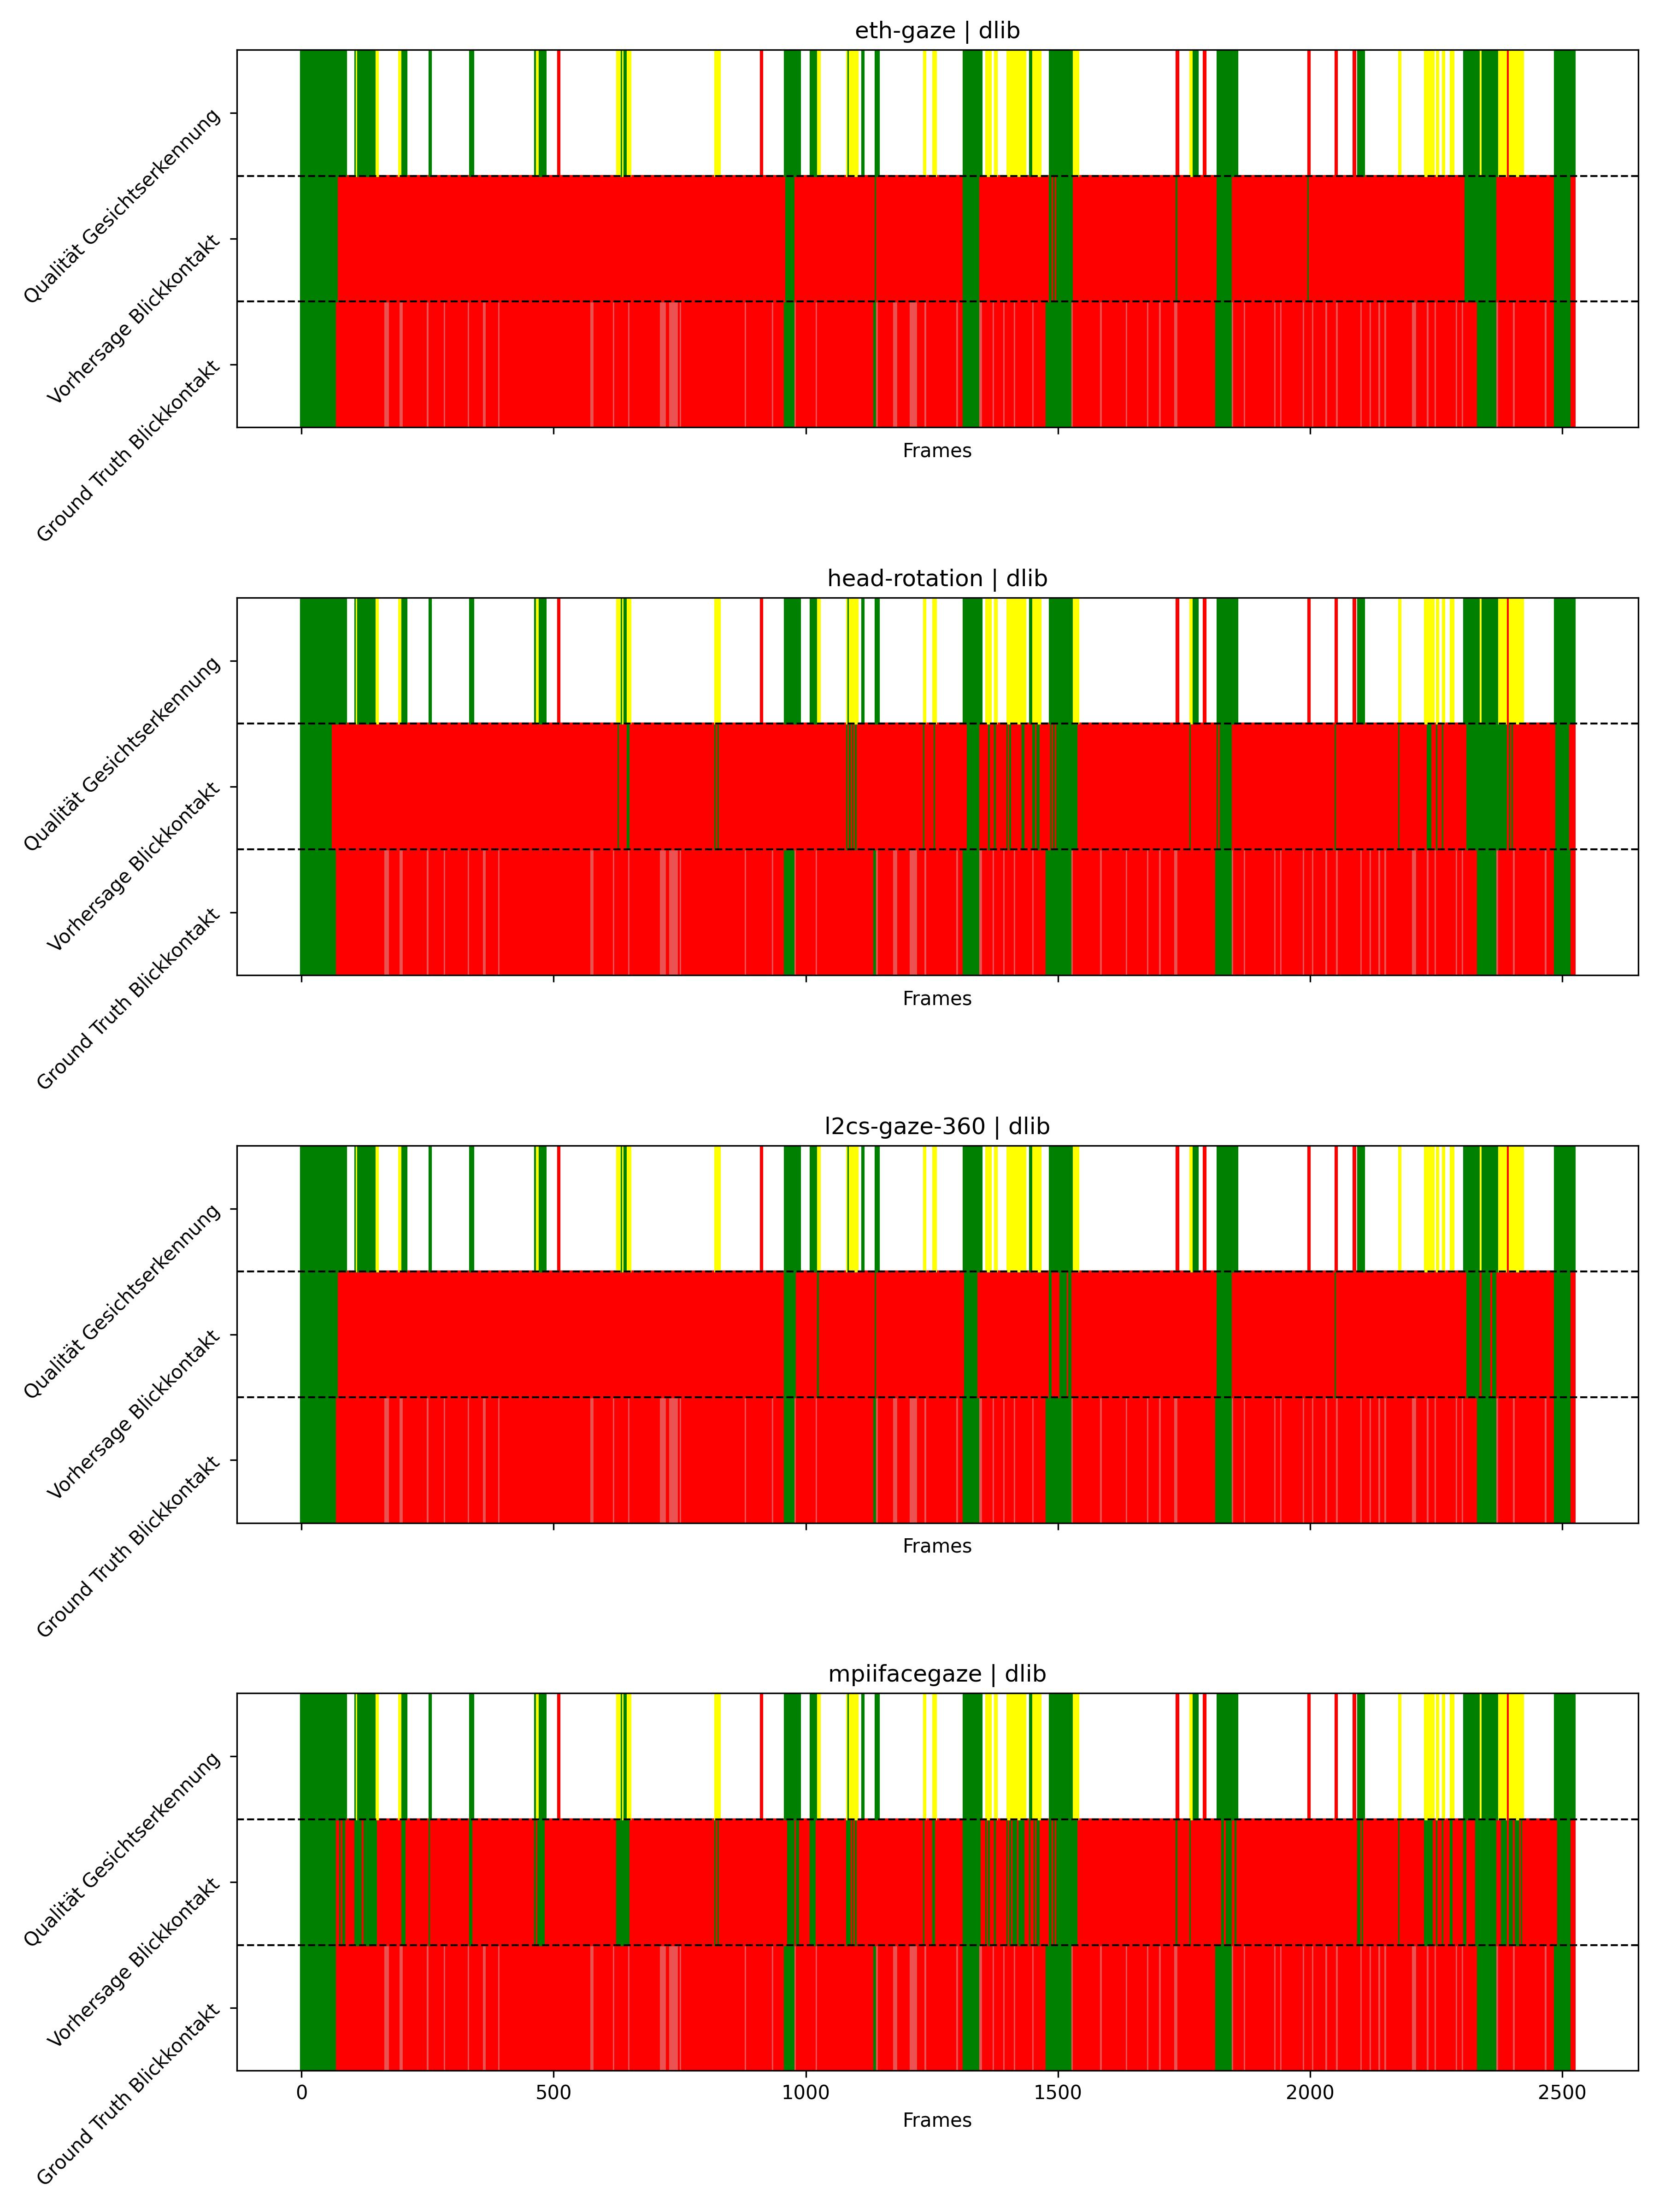
\includegraphics[width=1\linewidth]{appendix/18-dlib-overview-gaze.jpg}
\caption{Überblick über die Ground Truth des Blickkontakts, die Vorhersage des Blickkontakts und die Qualität der Gesichtserkennung mit \dlib. Die Bedeutung der Farben ist in Abbildung \ref{fig:evaluation:gaze:mpiifacegaze} erklärt.  }
\end{figure}

\begin{figure}[H]
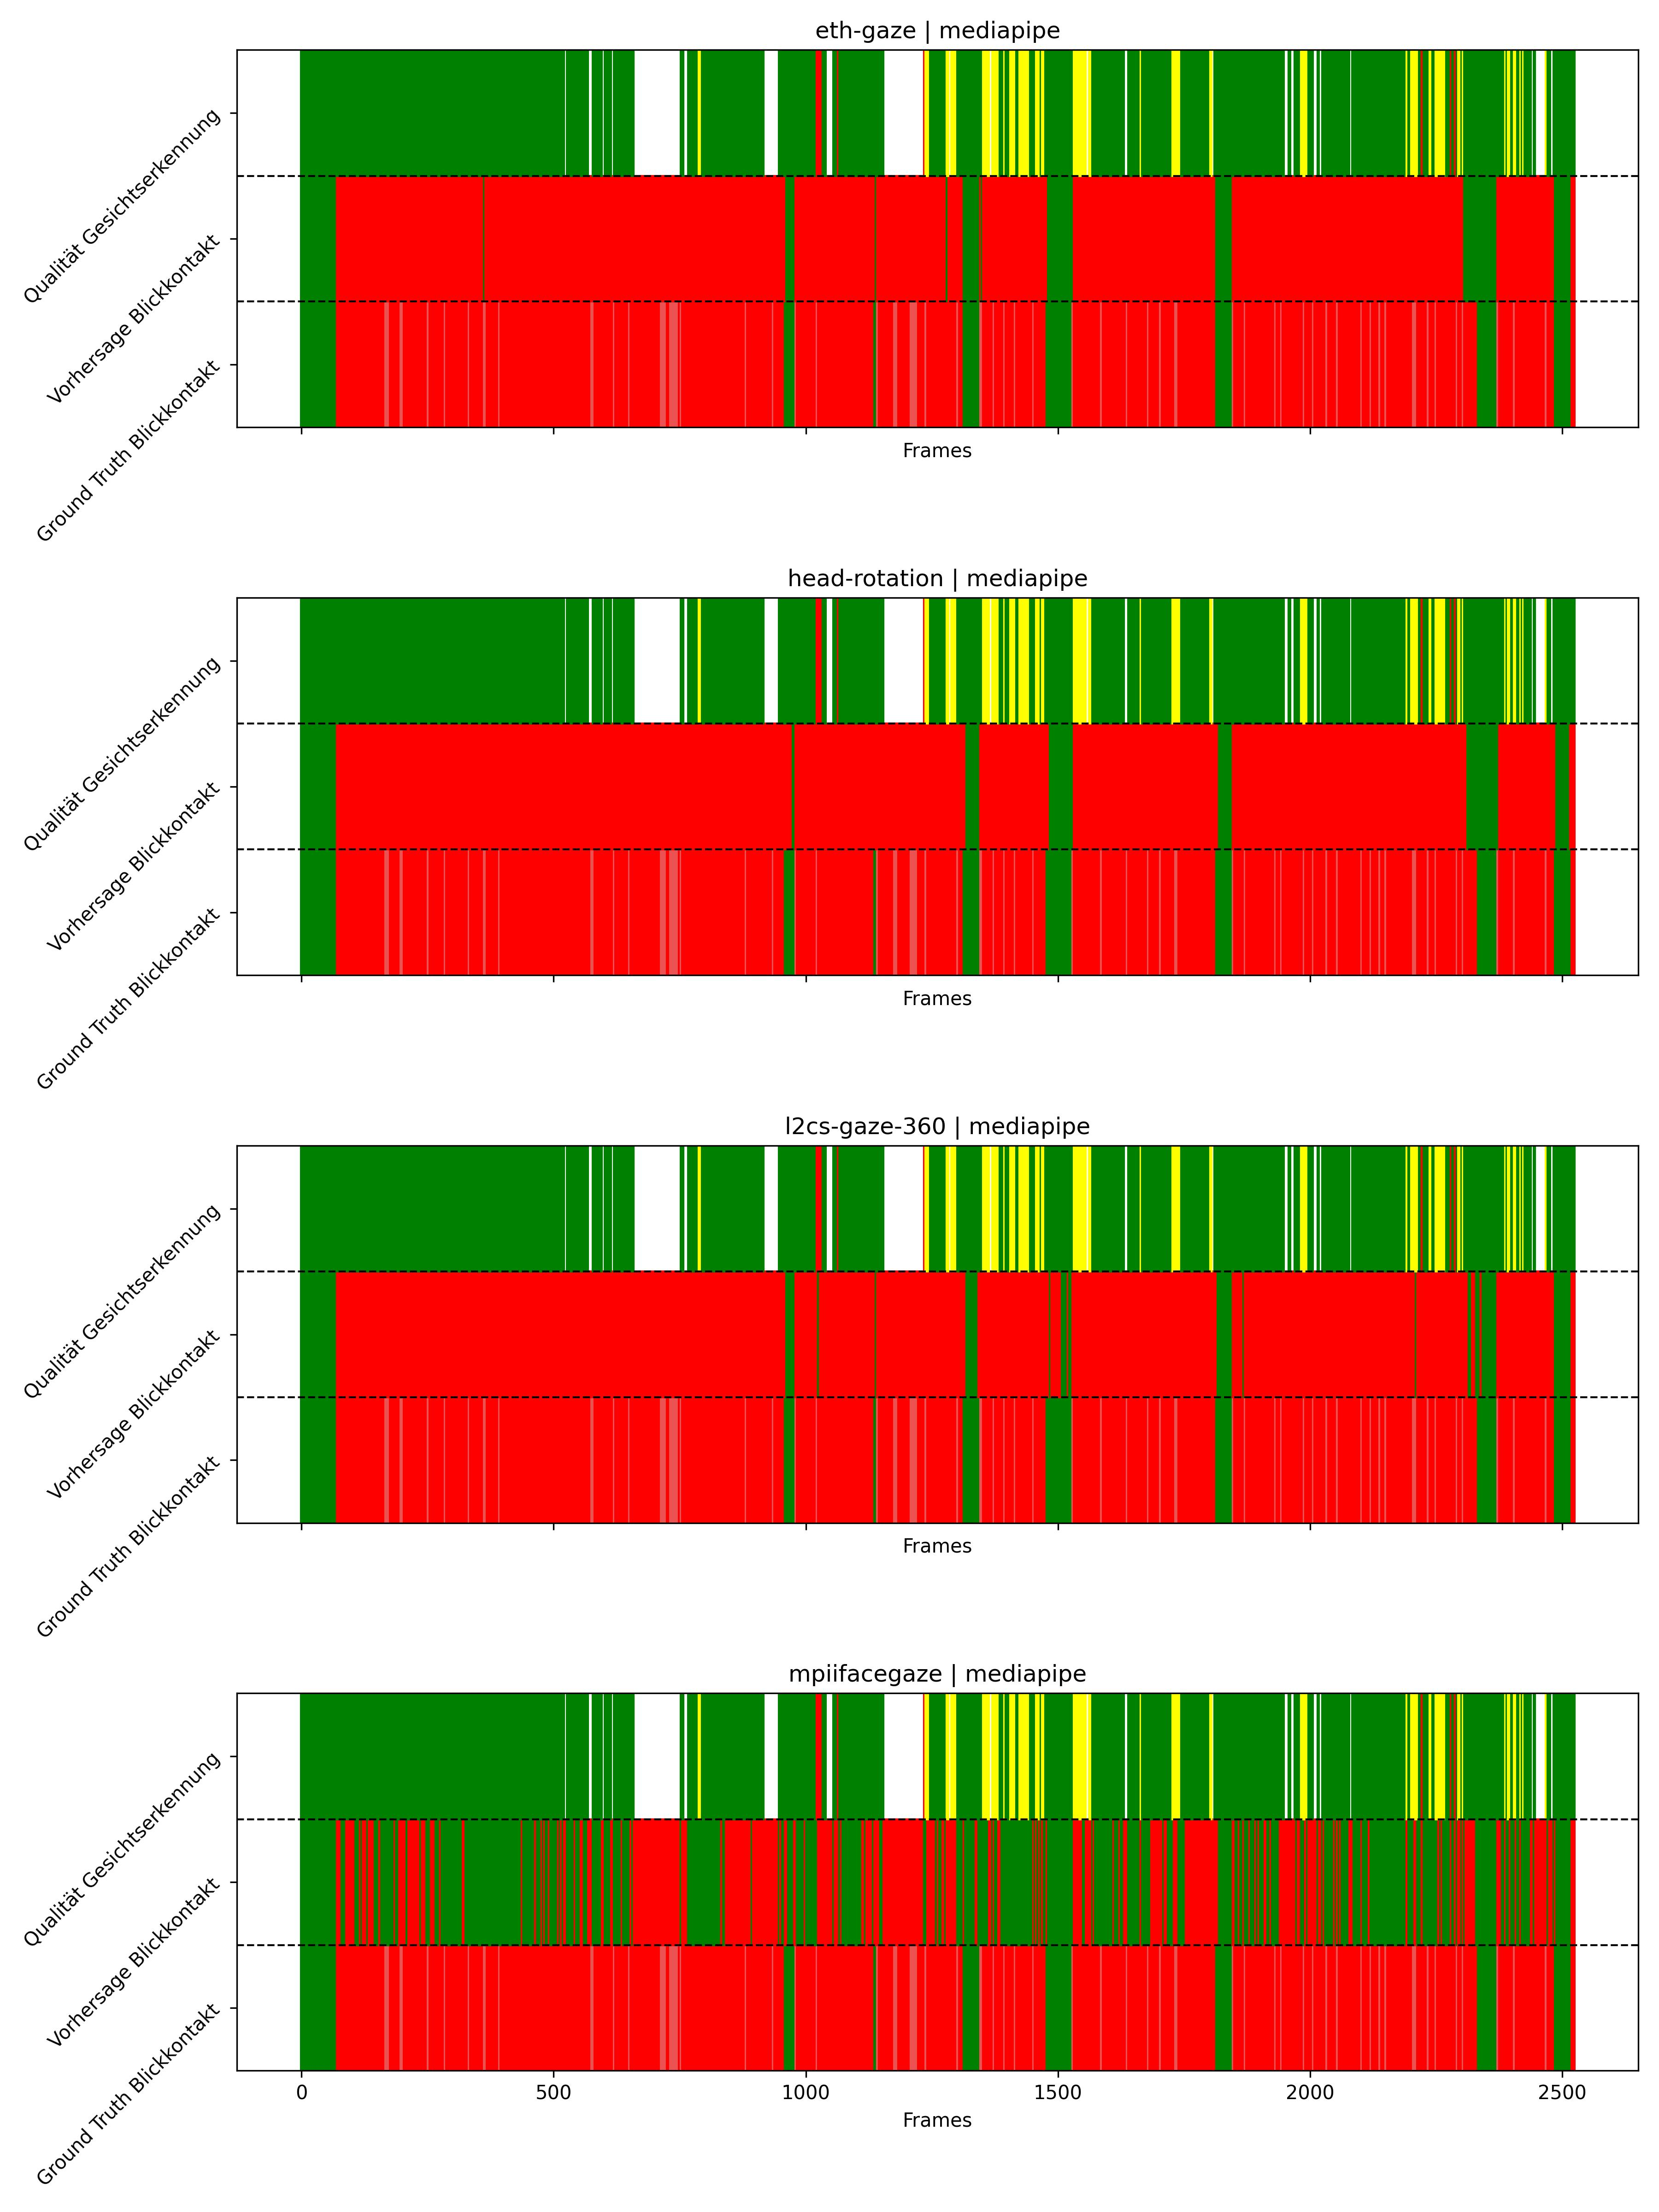
\includegraphics[width=1\linewidth]{appendix/18-mediapipe-overview-gaze.jpg}
\caption{Überblick über die Ground Truth des Blickkontakts, die Vorhersage des Blickkontakts und die Qualität der Gesichtserkennung mit \mediapipe. Die Bedeutung der Farben ist in Abbildung \ref{fig:evaluation:gaze:mpiifacegaze} erklärt.}
\end{figure}

\section{Video 19}
\begin{figure}[H]
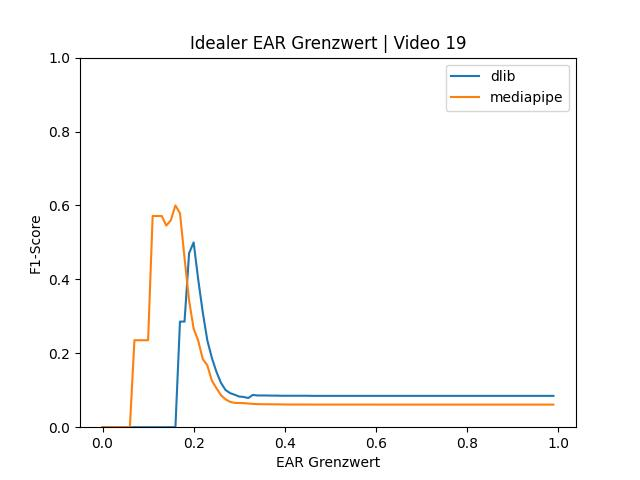
\includegraphics[width=0.7\linewidth]{appendix/19_f1-score-blink.jpg}
\caption{Ergebnisse der Bestimmung des idealen EAR-Grenzwerts für Video 19.}
\end{figure}

\begin{figure}[H]
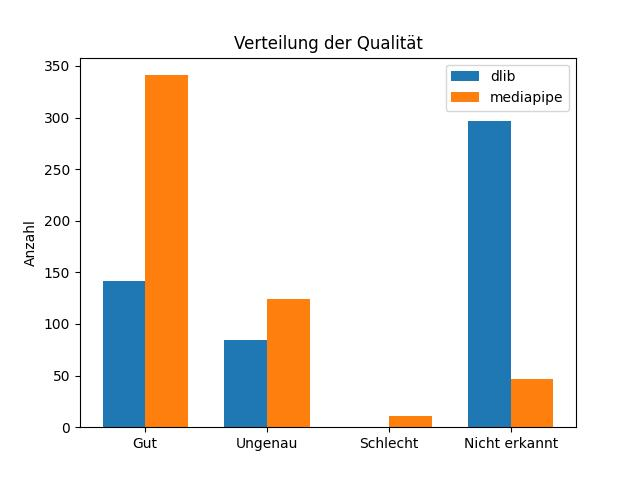
\includegraphics[width=0.7\linewidth]{appendix/19_bar-quality.jpg}
\caption{Aufteilung der Gesichtserkennungsqualität von Video 19.}
\end{figure}

\begin{table}[H]
\centering
\begin{tabular}{l|l|c c |c}
\toprule
\textbf{Gesichtserkennung} & \textbf{Blickrichtung} & \textbf{Seitenlänge} $\hitthresholdsize$ & \textbf{Verschiebung} $\hitthresholdposition$ & \textbf{F1-Score} \\ 
\midrule
\multirow{4}*{dlib}& ETH-XGaze & 0,153 & -0,002 & 0,972  \\ 
& Gaze360 & 0,398 & 0,01 & 0,961 \\ 
& MPIIFaceGaze & 0,112 & 0,059 & 0,678  \\ 
& Kopfrotation & 0,163 & 0,194 & 0,74  \\ 
\hline\multirow{4}*{MediaPipe}& ETH-XGaze & 0,143 & -0,002 & 0,971  \\ 
& Gaze360 & 0,398 & 0,022 & 0,956 \\ 
& MPIIFaceGaze & 0,031 & -0,027 & 0,56  \\ 
& Kopfrotation & 0,122 & 0,194 & 0,87  \\ 
\bottomrule\end{tabular}
\caption{Ergebnis des Hyperparameter-Tunings für die Zone speziell für Video 19.}
\label{tab:appendix:19:local}
\end{table}
\begin{table}[H]
\centering
\begin{tabular}{l|l|c c c c|c c|c}
\toprule
\textbf{Gesichtserkennung} & \textbf{Blickrichtung} & $TP$ & $TN$& $FP$ & $FN$ & \textbf{Precision} & \textbf{Recall} & \textbf{F1-Score} \\ 
\midrule
\multirow{4}*{dlib}& ETH-XGaze & 87 & 428 & 7 & 1 & 0,926 & 0,989 & 0,956 \\ 
& Gaze360 & 87 & 424 & 11 & 1 & 0,888 & 0,989 & 0,935 \\ 
& MPIIFaceGaze & 79 & 316 & 119 & 9 & 0,399 & 0,898 & 0,552 \\ 
& Kopfrotation & 81 & 384 & 51 & 7 & 0,614 & 0,92 & 0,736 \\ 
\hline\multirow{4}*{MediaPipe}& ETH-XGaze & 87 & 426 & 9 & 1 & 0,906 & 0,989 & 0,946 \\ 
& Gaze360 & 87 & 424 & 11 & 1 & 0,888 & 0,989 & 0,935 \\ 
& MPIIFaceGaze & 81 & 223 & 212 & 7 & 0,276 & 0,92 & 0,425 \\ 
& Kopfrotation & 84 & 408 & 27 & 4 & 0,757 & 0,955 & 0,844 \\ 
\bottomrule\end{tabular}
\caption{Zusammensetzung des F1-Scores unter Verwendung der in Kapitel \ref{sec:evaluation:results:gaze:threshold} bestimmten globalen Parameter $\hitthresholdsize$ und $\hitthresholdposition$.}
\label{tab:appendix:19:f1}
\end{table}
\begin{figure}[H]
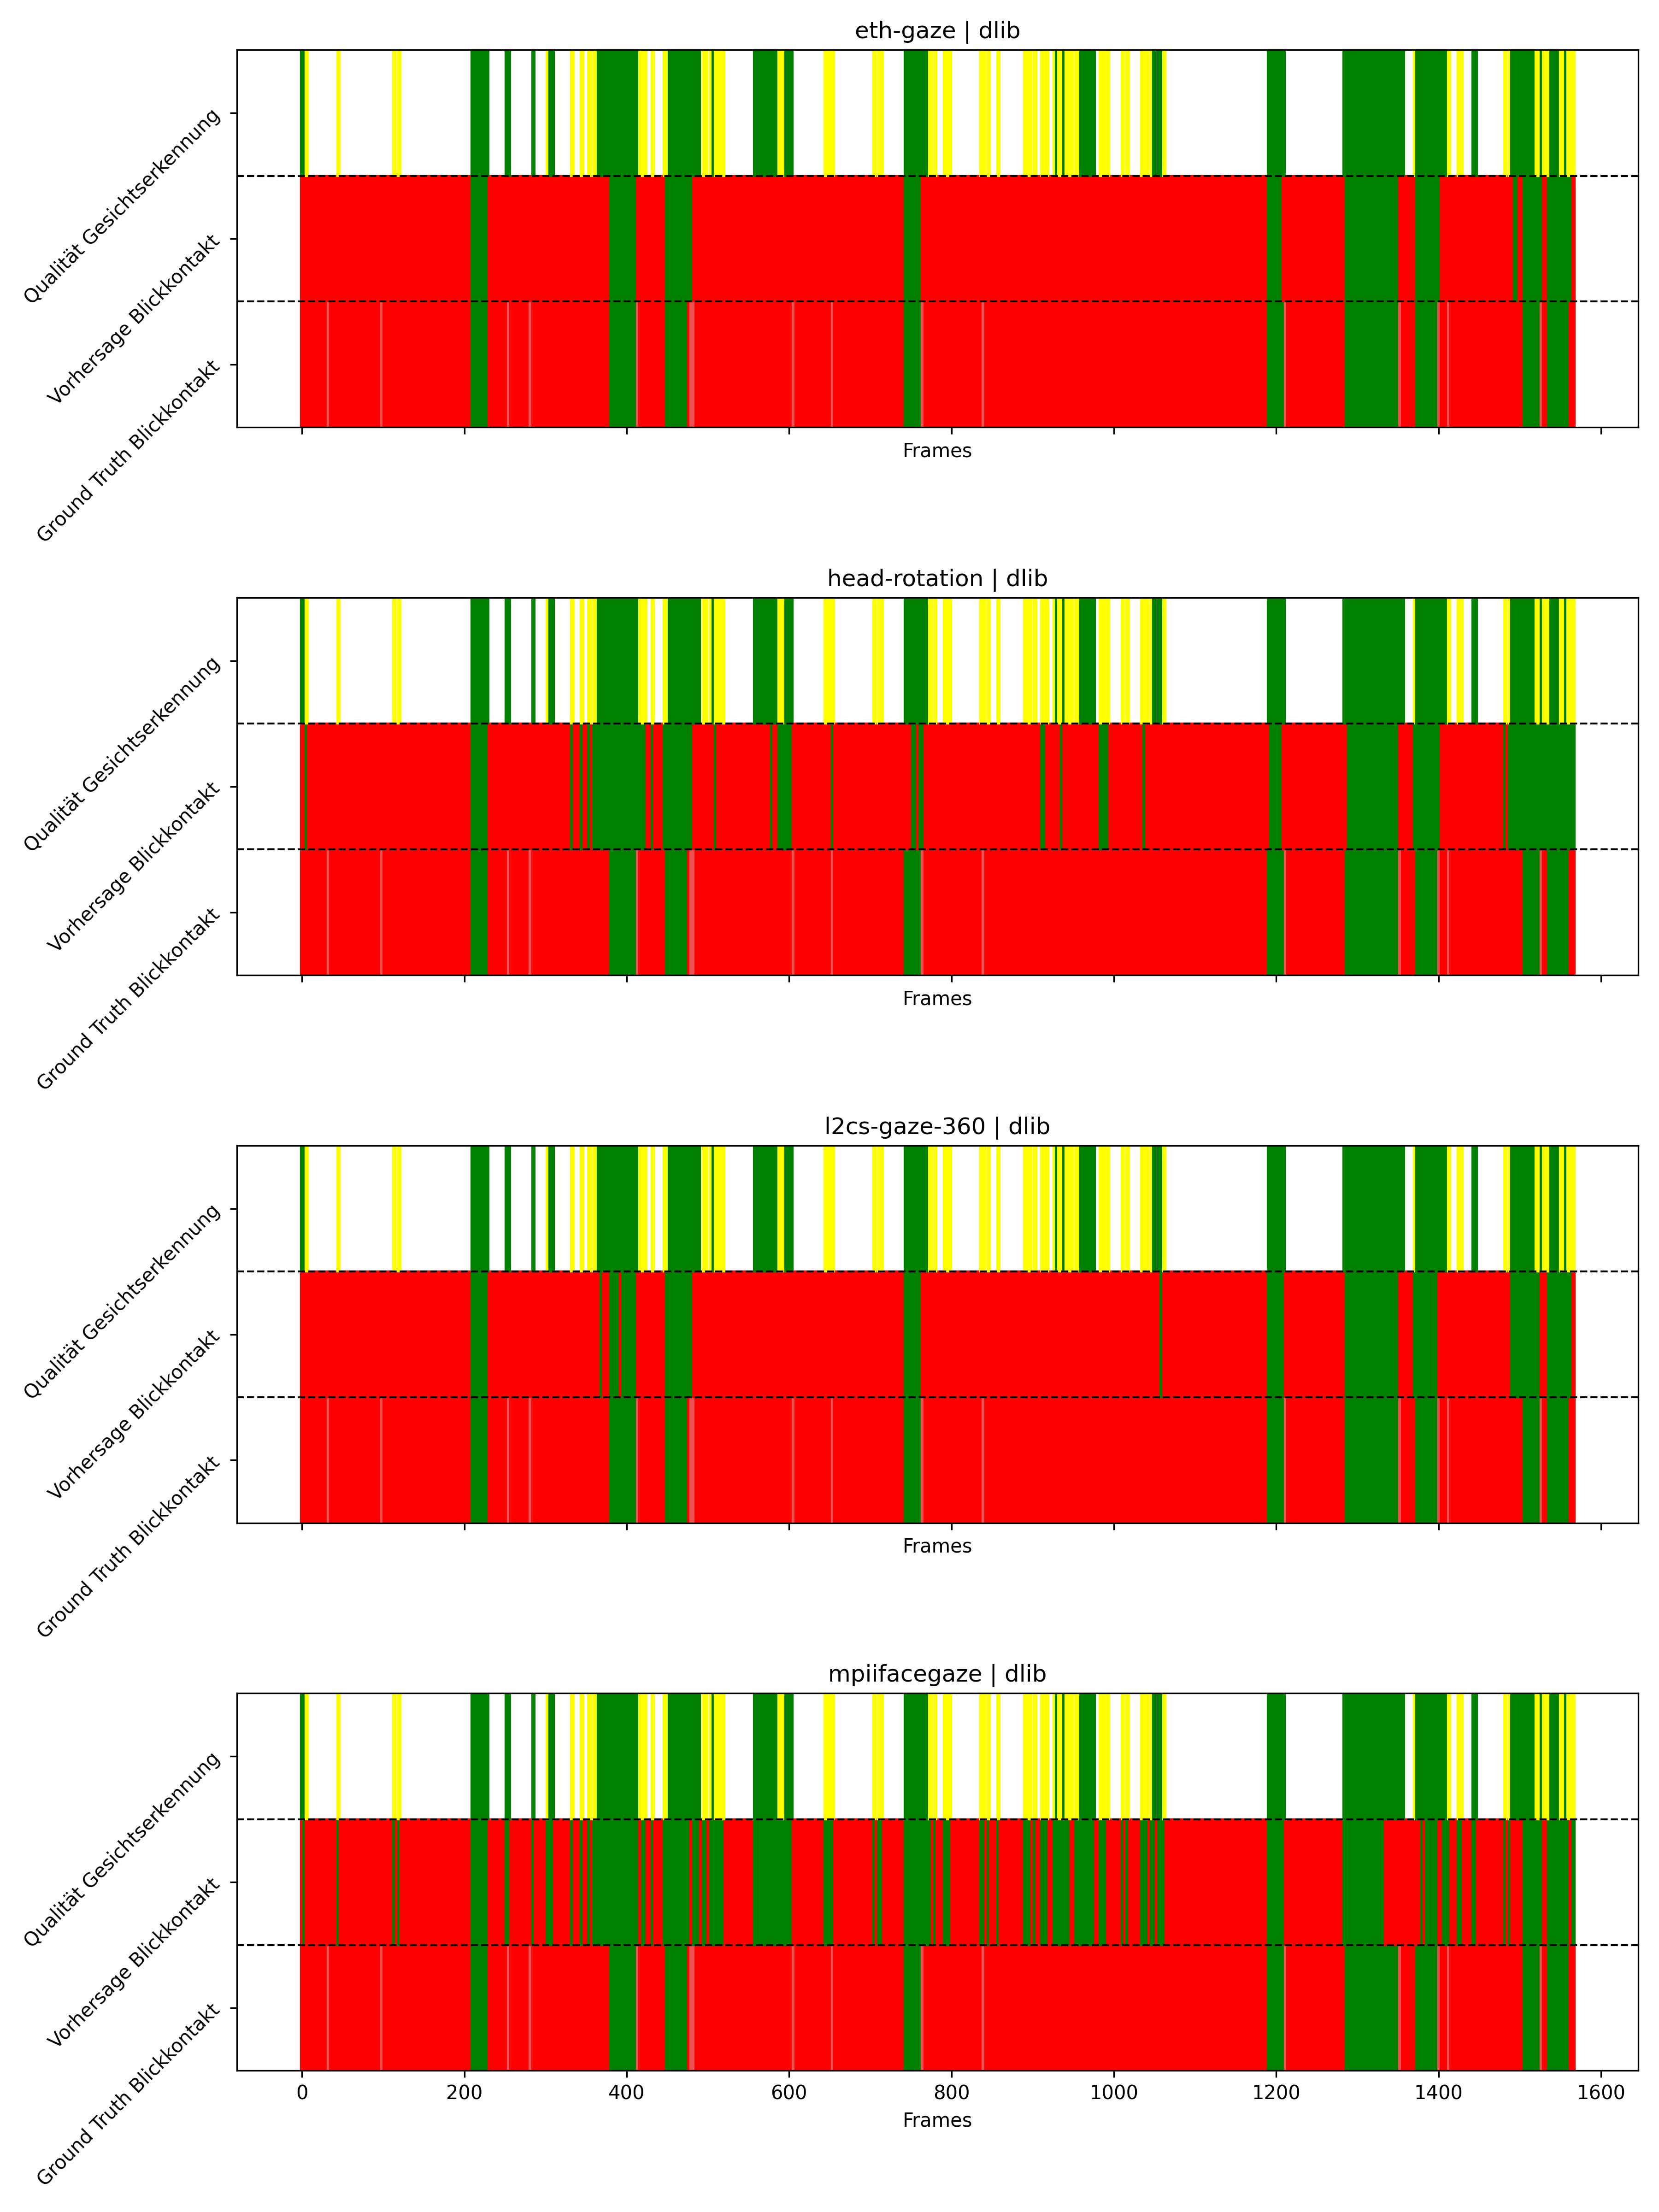
\includegraphics[width=1\linewidth]{appendix/19-dlib-overview-gaze.jpg}
\caption{Überblick über die Ground Truth des Blickkontakts, die Vorhersage des Blickkontakts und die Qualität der Gesichtserkennung mit \dlib. Die Bedeutung der Farben ist in Abbildung \ref{fig:evaluation:gaze:mpiifacegaze} erklärt.  }
\end{figure}

\begin{figure}[H]
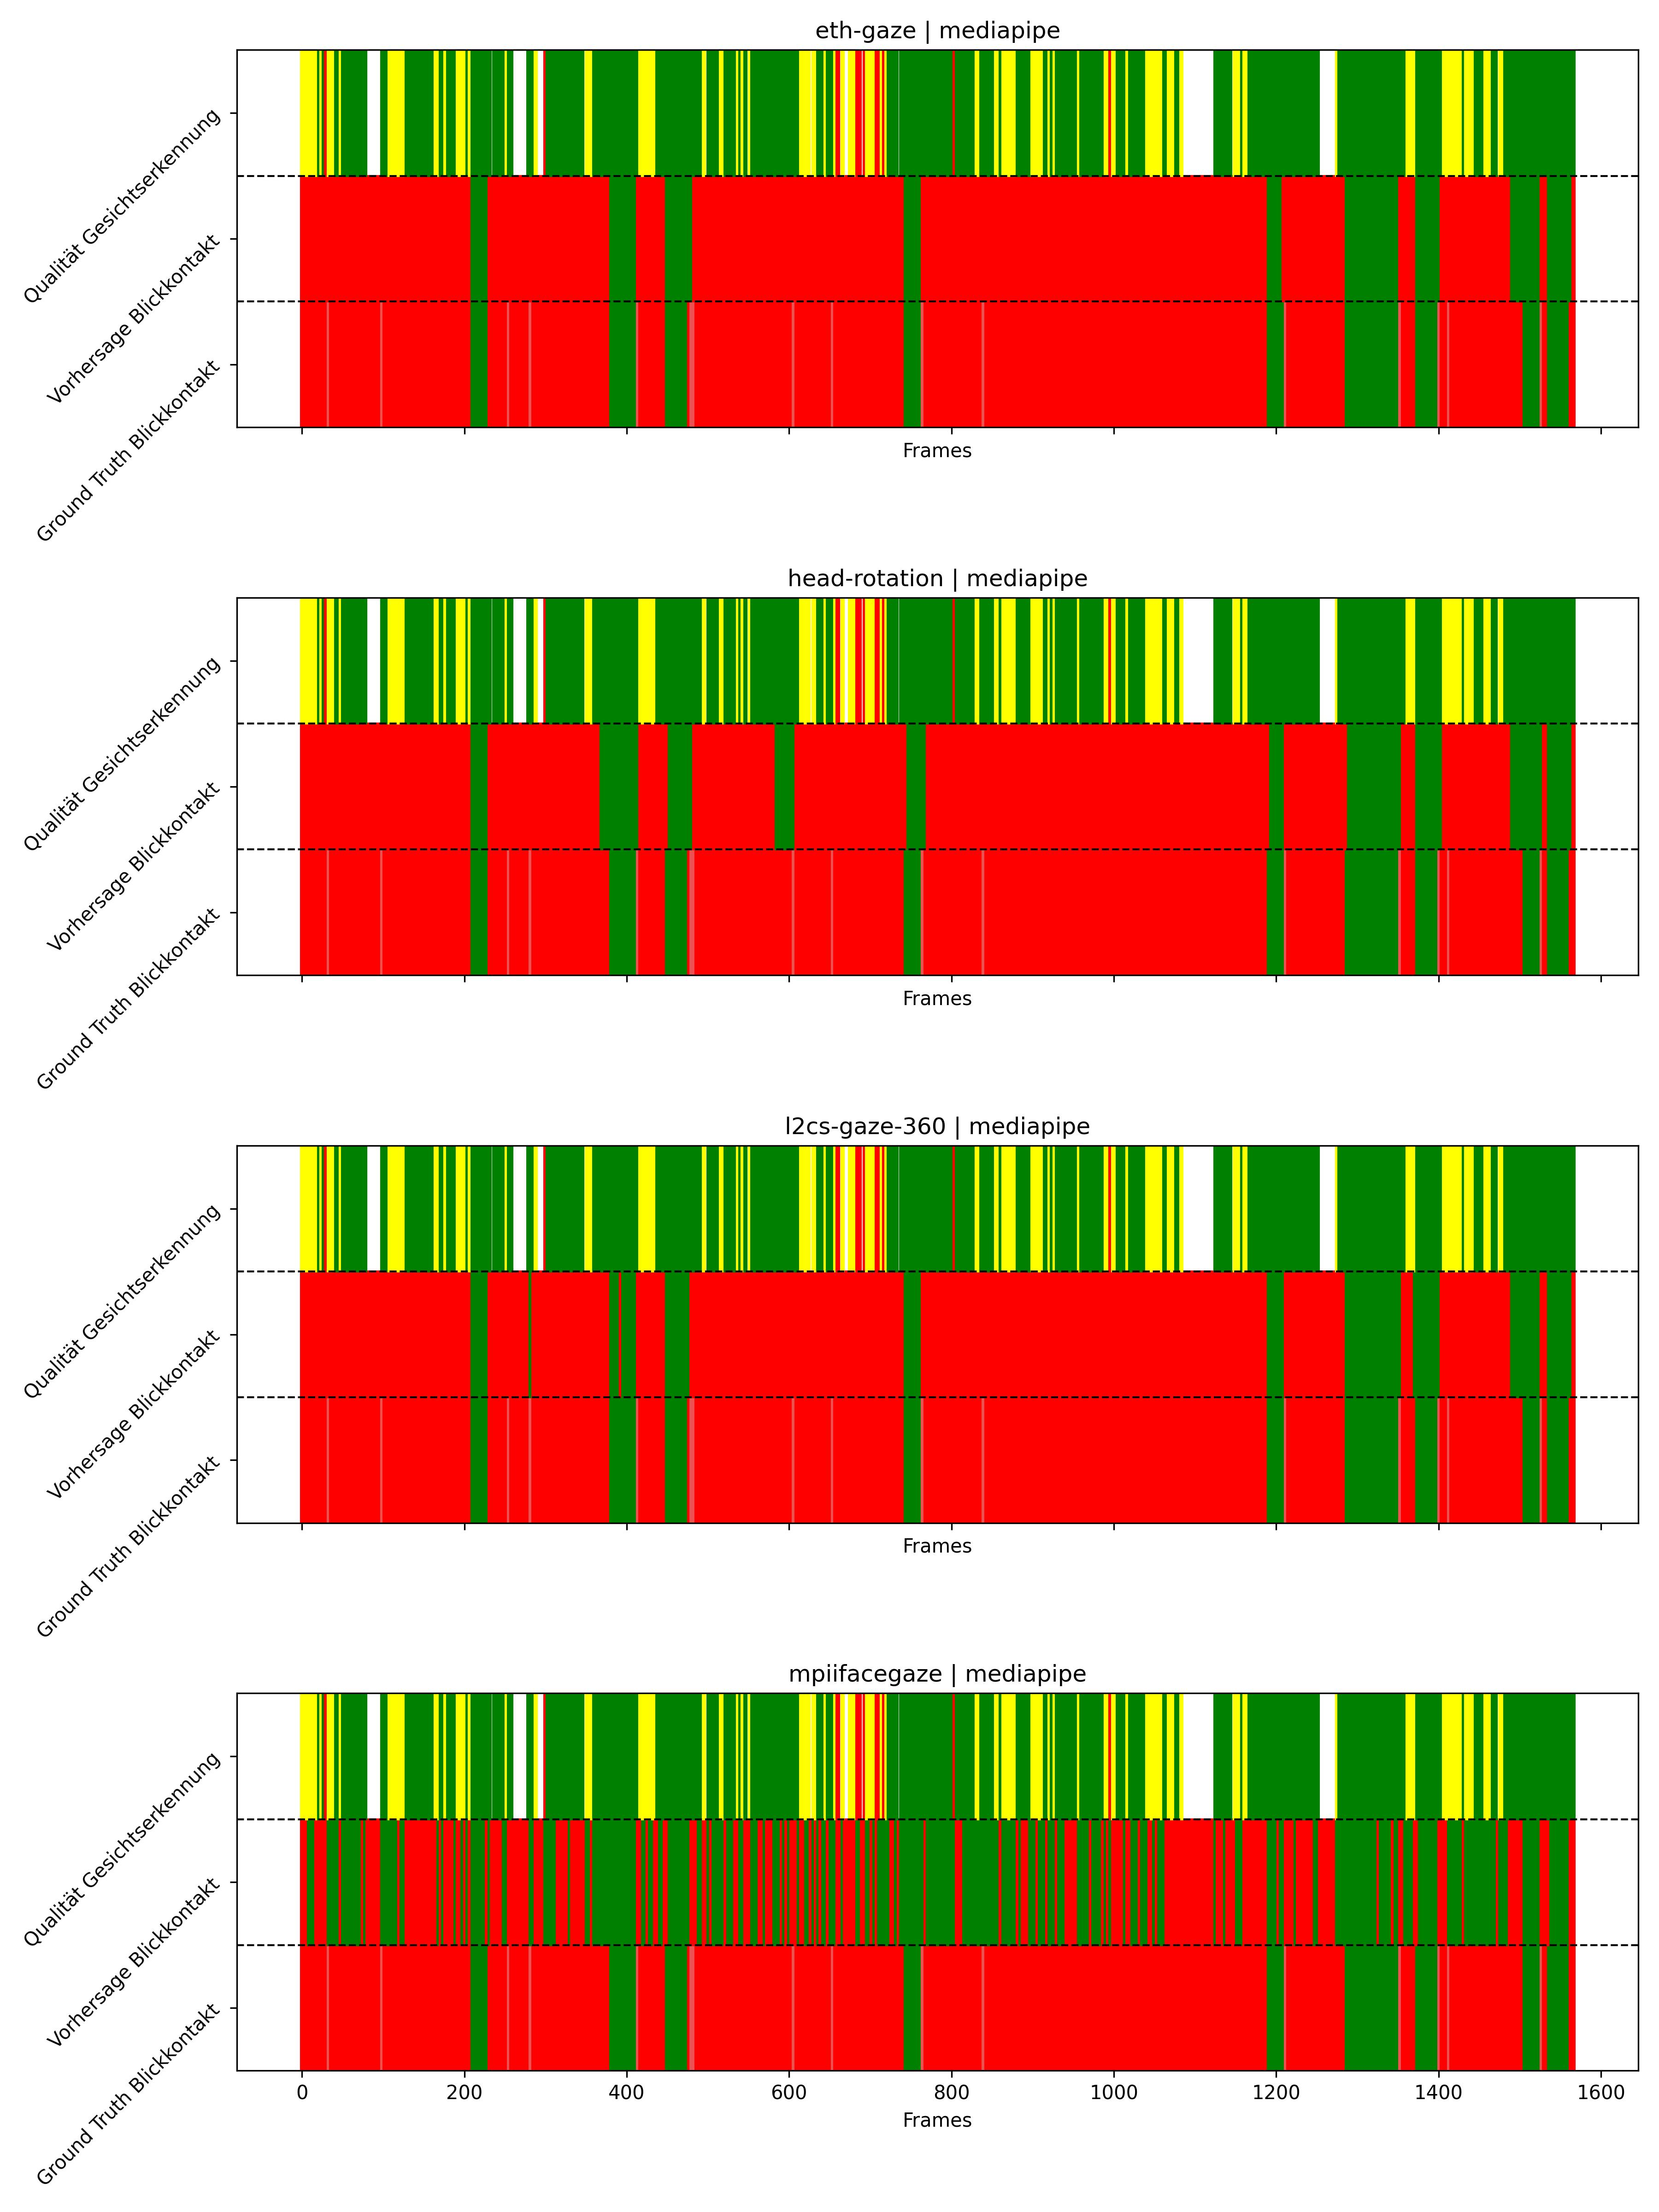
\includegraphics[width=1\linewidth]{appendix/19-mediapipe-overview-gaze.jpg}
\caption{Überblick über die Ground Truth des Blickkontakts, die Vorhersage des Blickkontakts und die Qualität der Gesichtserkennung mit \mediapipe. Die Bedeutung der Farben ist in Abbildung \ref{fig:evaluation:gaze:mpiifacegaze} erklärt.}
\end{figure}

\section{Video 20}
\begin{figure}[H]
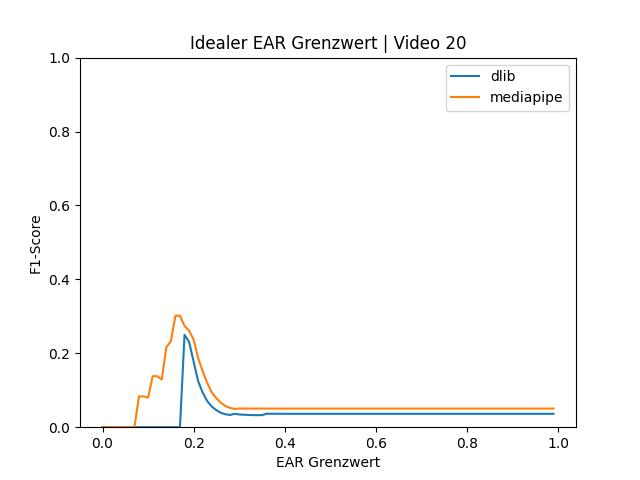
\includegraphics[width=0.7\linewidth]{appendix/20_f1-score-blink.jpg}
\caption{Ergebnisse der Bestimmung des idealen EAR-Grenzwerts für Video 20.}
\end{figure}

\begin{figure}[H]
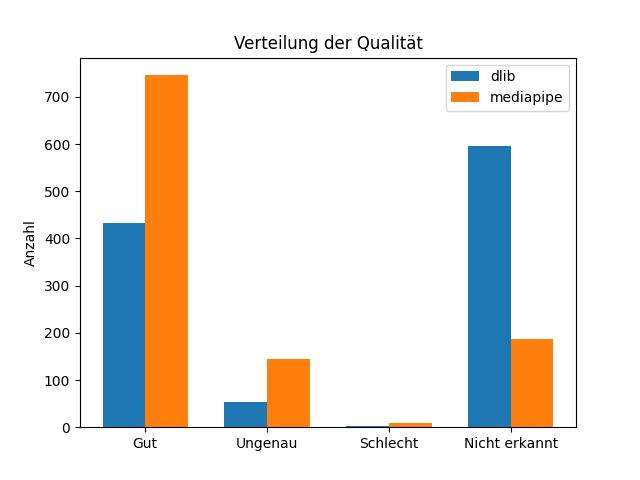
\includegraphics[width=0.7\linewidth]{appendix/20_bar-quality.jpg}
\caption{Aufteilung der Gesichtserkennungsqualität von Video 20.}
\end{figure}

\begin{table}[H]
\centering
\begin{tabular}{l|l|c c |c}
\toprule
\textbf{Gesichtserkennung} & \textbf{Blickrichtung} & \textbf{Seitenlänge} $\hitthresholdsize$ & \textbf{Verschiebung} $\hitthresholdposition$ & \textbf{F1-Score} \\ 
\midrule
\multirow{4}*{dlib}& ETH-XGaze & 0,173 & -0,002 & 0,945  \\ 
& Gaze360 & 0,49 & 0,035 & 0,895 \\ 
& MPIIFaceGaze & 0,051 & -0,027 & 0,795  \\ 
& Kopfrotation & 0,173 & 0,218 & 0,78  \\ 
\hline\multirow{4}*{MediaPipe}& ETH-XGaze & 0,173 & -0,014 & 0,961  \\ 
& Gaze360 & 0,296 & 0,035 & 0,895 \\ 
& MPIIFaceGaze & 0,041 & -0,039 & 0,596  \\ 
& Kopfrotation & 0,163 & 0,194 & 0,803  \\ 
\bottomrule\end{tabular}
\caption{Ergebnis des Hyperparameter-Tunings für die Zone speziell für Video 20.}
\label{tab:appendix:20:local}
\end{table}
\begin{table}[H]
\centering
\begin{tabular}{l|l|c c c c|c c|c}
\toprule
\textbf{Gesichtserkennung} & \textbf{Blickrichtung} & $TP$ & $TN$& $FP$ & $FN$ & \textbf{Precision} & \textbf{Recall} & \textbf{F1-Score} \\ 
\midrule
\multirow{4}*{dlib}& ETH-XGaze & 294 & 745 & 20 & 23 & 0,936 & 0,927 & 0,932 \\ 
& Gaze360 & 290 & 716 & 49 & 27 & 0,855 & 0,915 & 0,884 \\ 
& MPIIFaceGaze & 299 & 624 & 141 & 18 & 0,68 & 0,943 & 0,79 \\ 
& Kopfrotation & 264 & 654 & 111 & 53 & 0,704 & 0,833 & 0,763 \\ 
\hline\multirow{4}*{MediaPipe}& ETH-XGaze & 314 & 725 & 41 & 4 & 0,885 & 0,987 & 0,933 \\ 
& Gaze360 & 305 & 696 & 70 & 13 & 0,813 & 0,959 & 0,88 \\ 
& MPIIFaceGaze & 304 & 354 & 412 & 14 & 0,425 & 0,956 & 0,588 \\ 
& Kopfrotation & 291 & 638 & 128 & 27 & 0,695 & 0,915 & 0,79 \\ 
\bottomrule\end{tabular}
\caption{Zusammensetzung des F1-Scores unter Verwendung der in Kapitel \ref{sec:evaluation:results:gaze:threshold} bestimmten globalen Parameter $\hitthresholdsize$ und $\hitthresholdposition$.}
\label{tab:appendix:20:f1}
\end{table}
\begin{figure}[H]
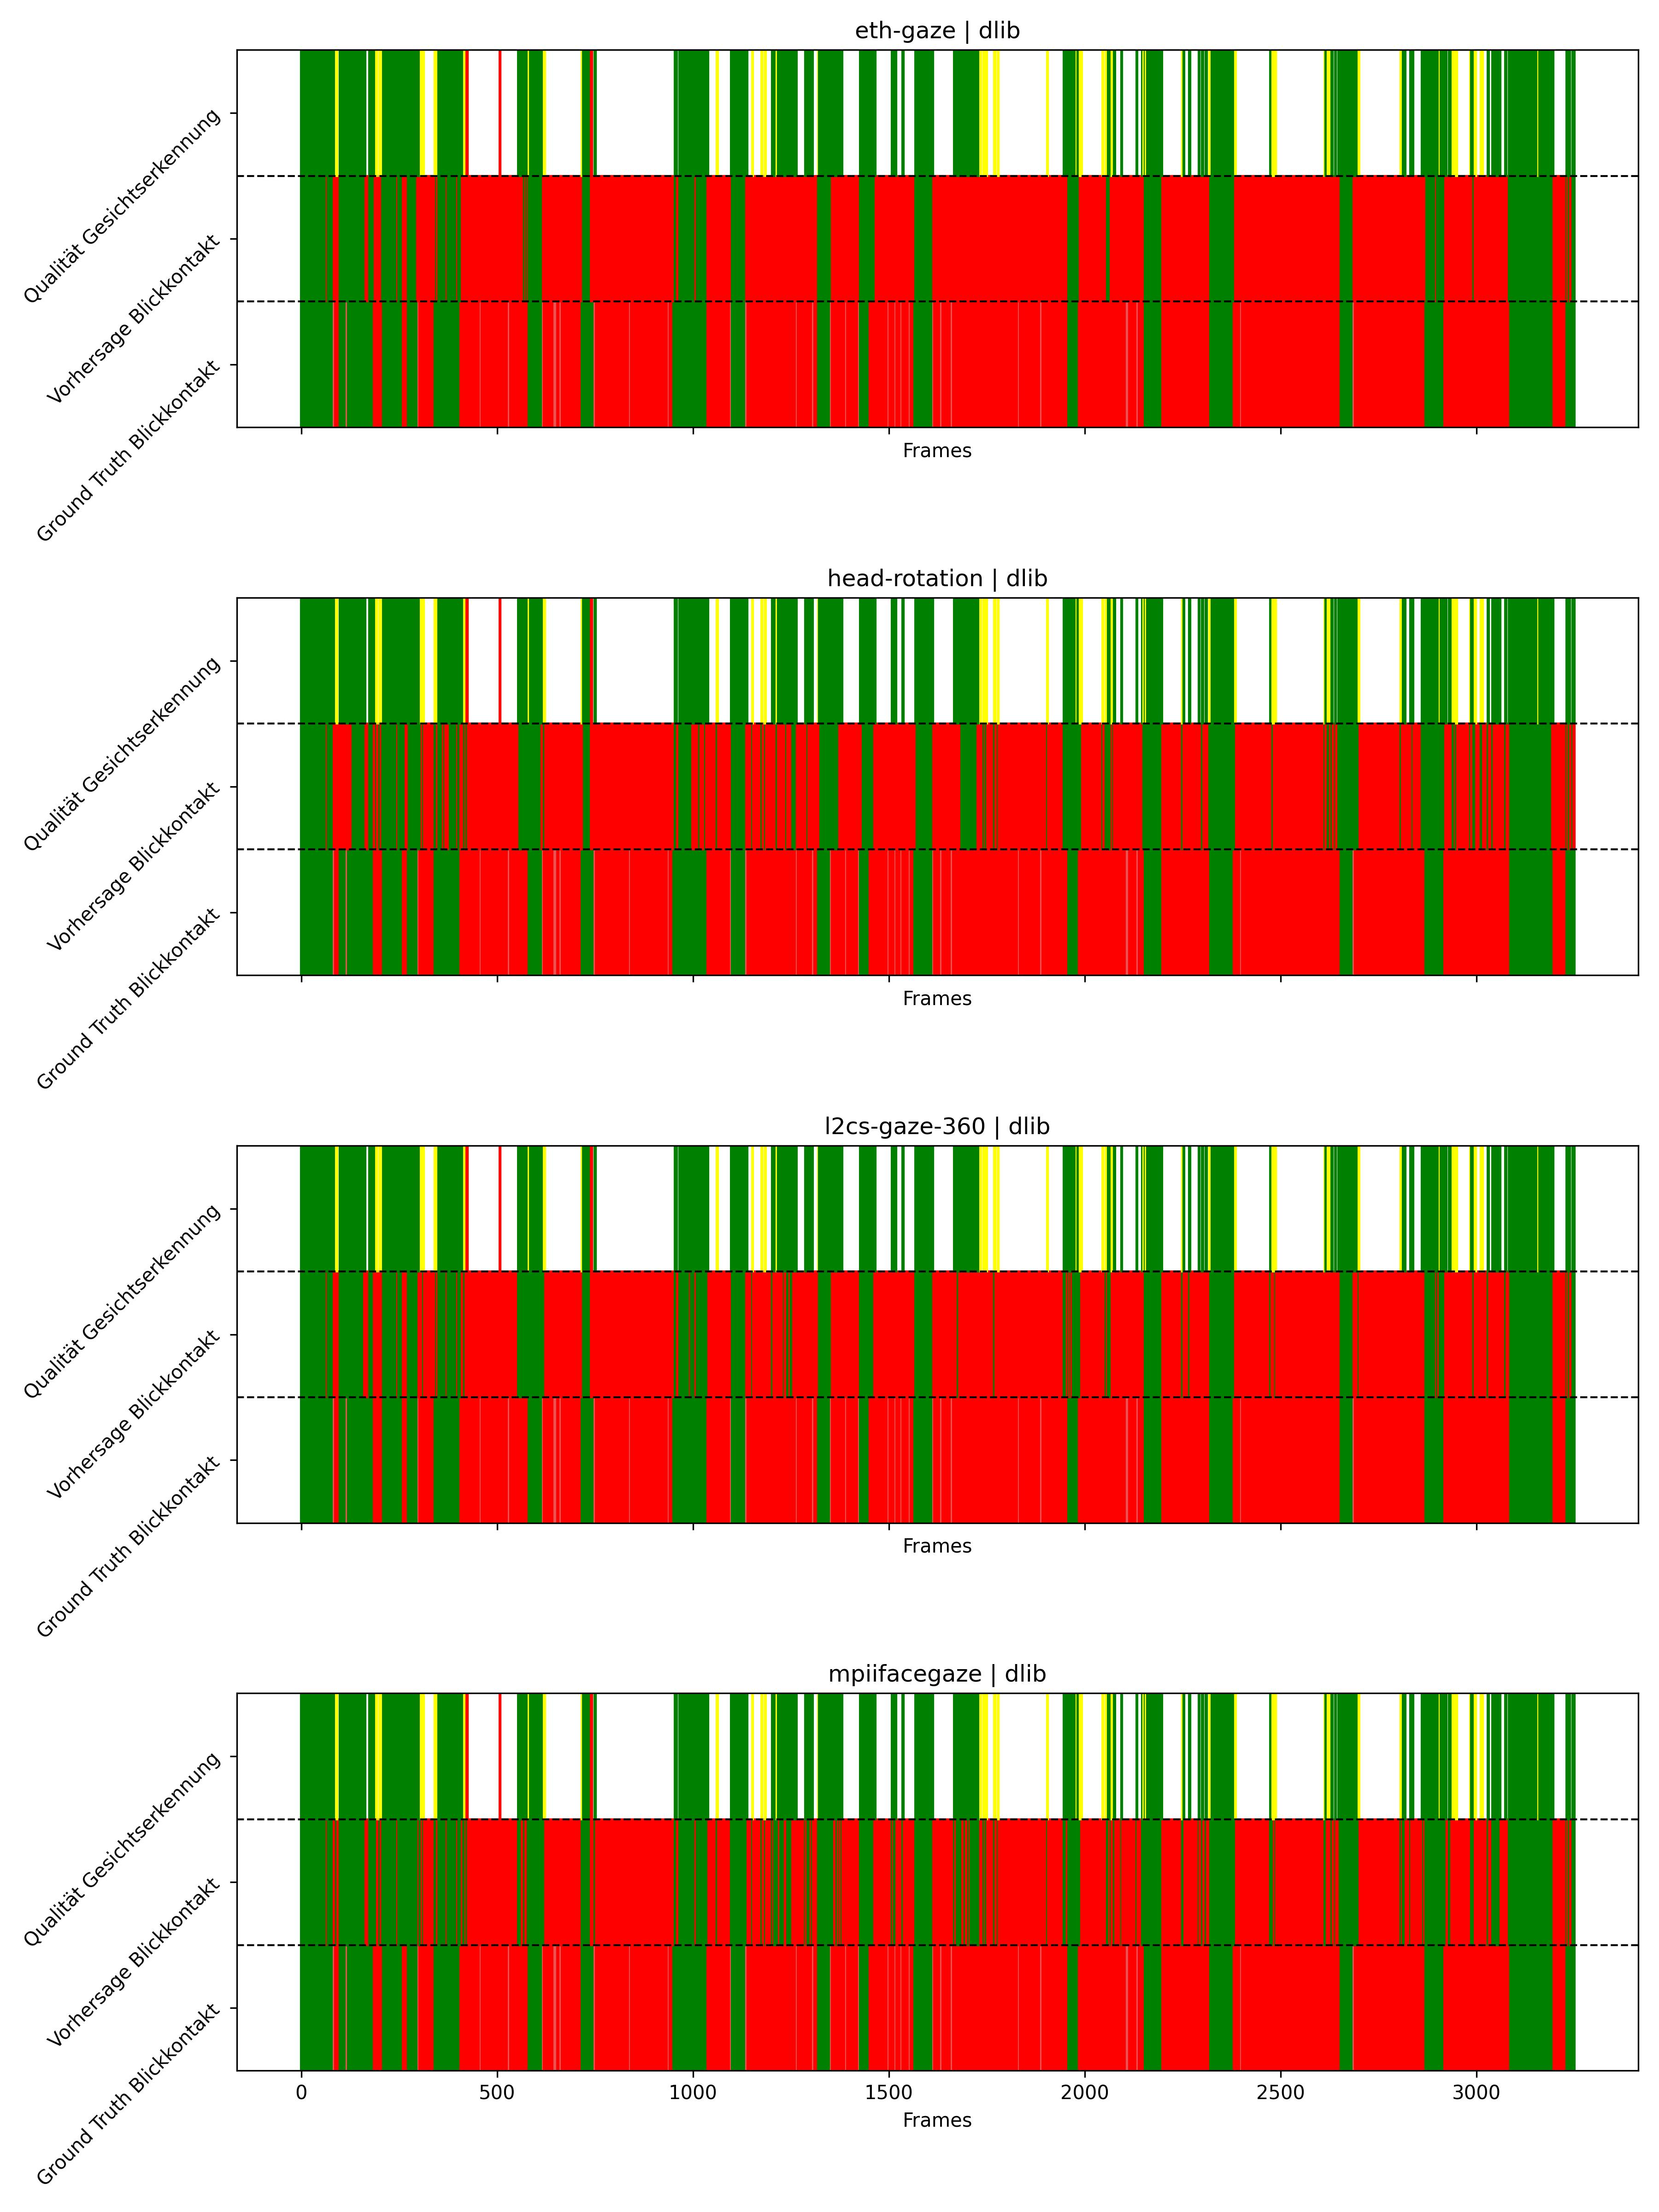
\includegraphics[width=1\linewidth]{appendix/20-dlib-overview-gaze.jpg}
\caption{Überblick über die Ground Truth des Blickkontakts, die Vorhersage des Blickkontakts und die Qualität der Gesichtserkennung mit \dlib. Die Bedeutung der Farben ist in Abbildung \ref{fig:evaluation:gaze:mpiifacegaze} erklärt.  }
\end{figure}

\begin{figure}[H]
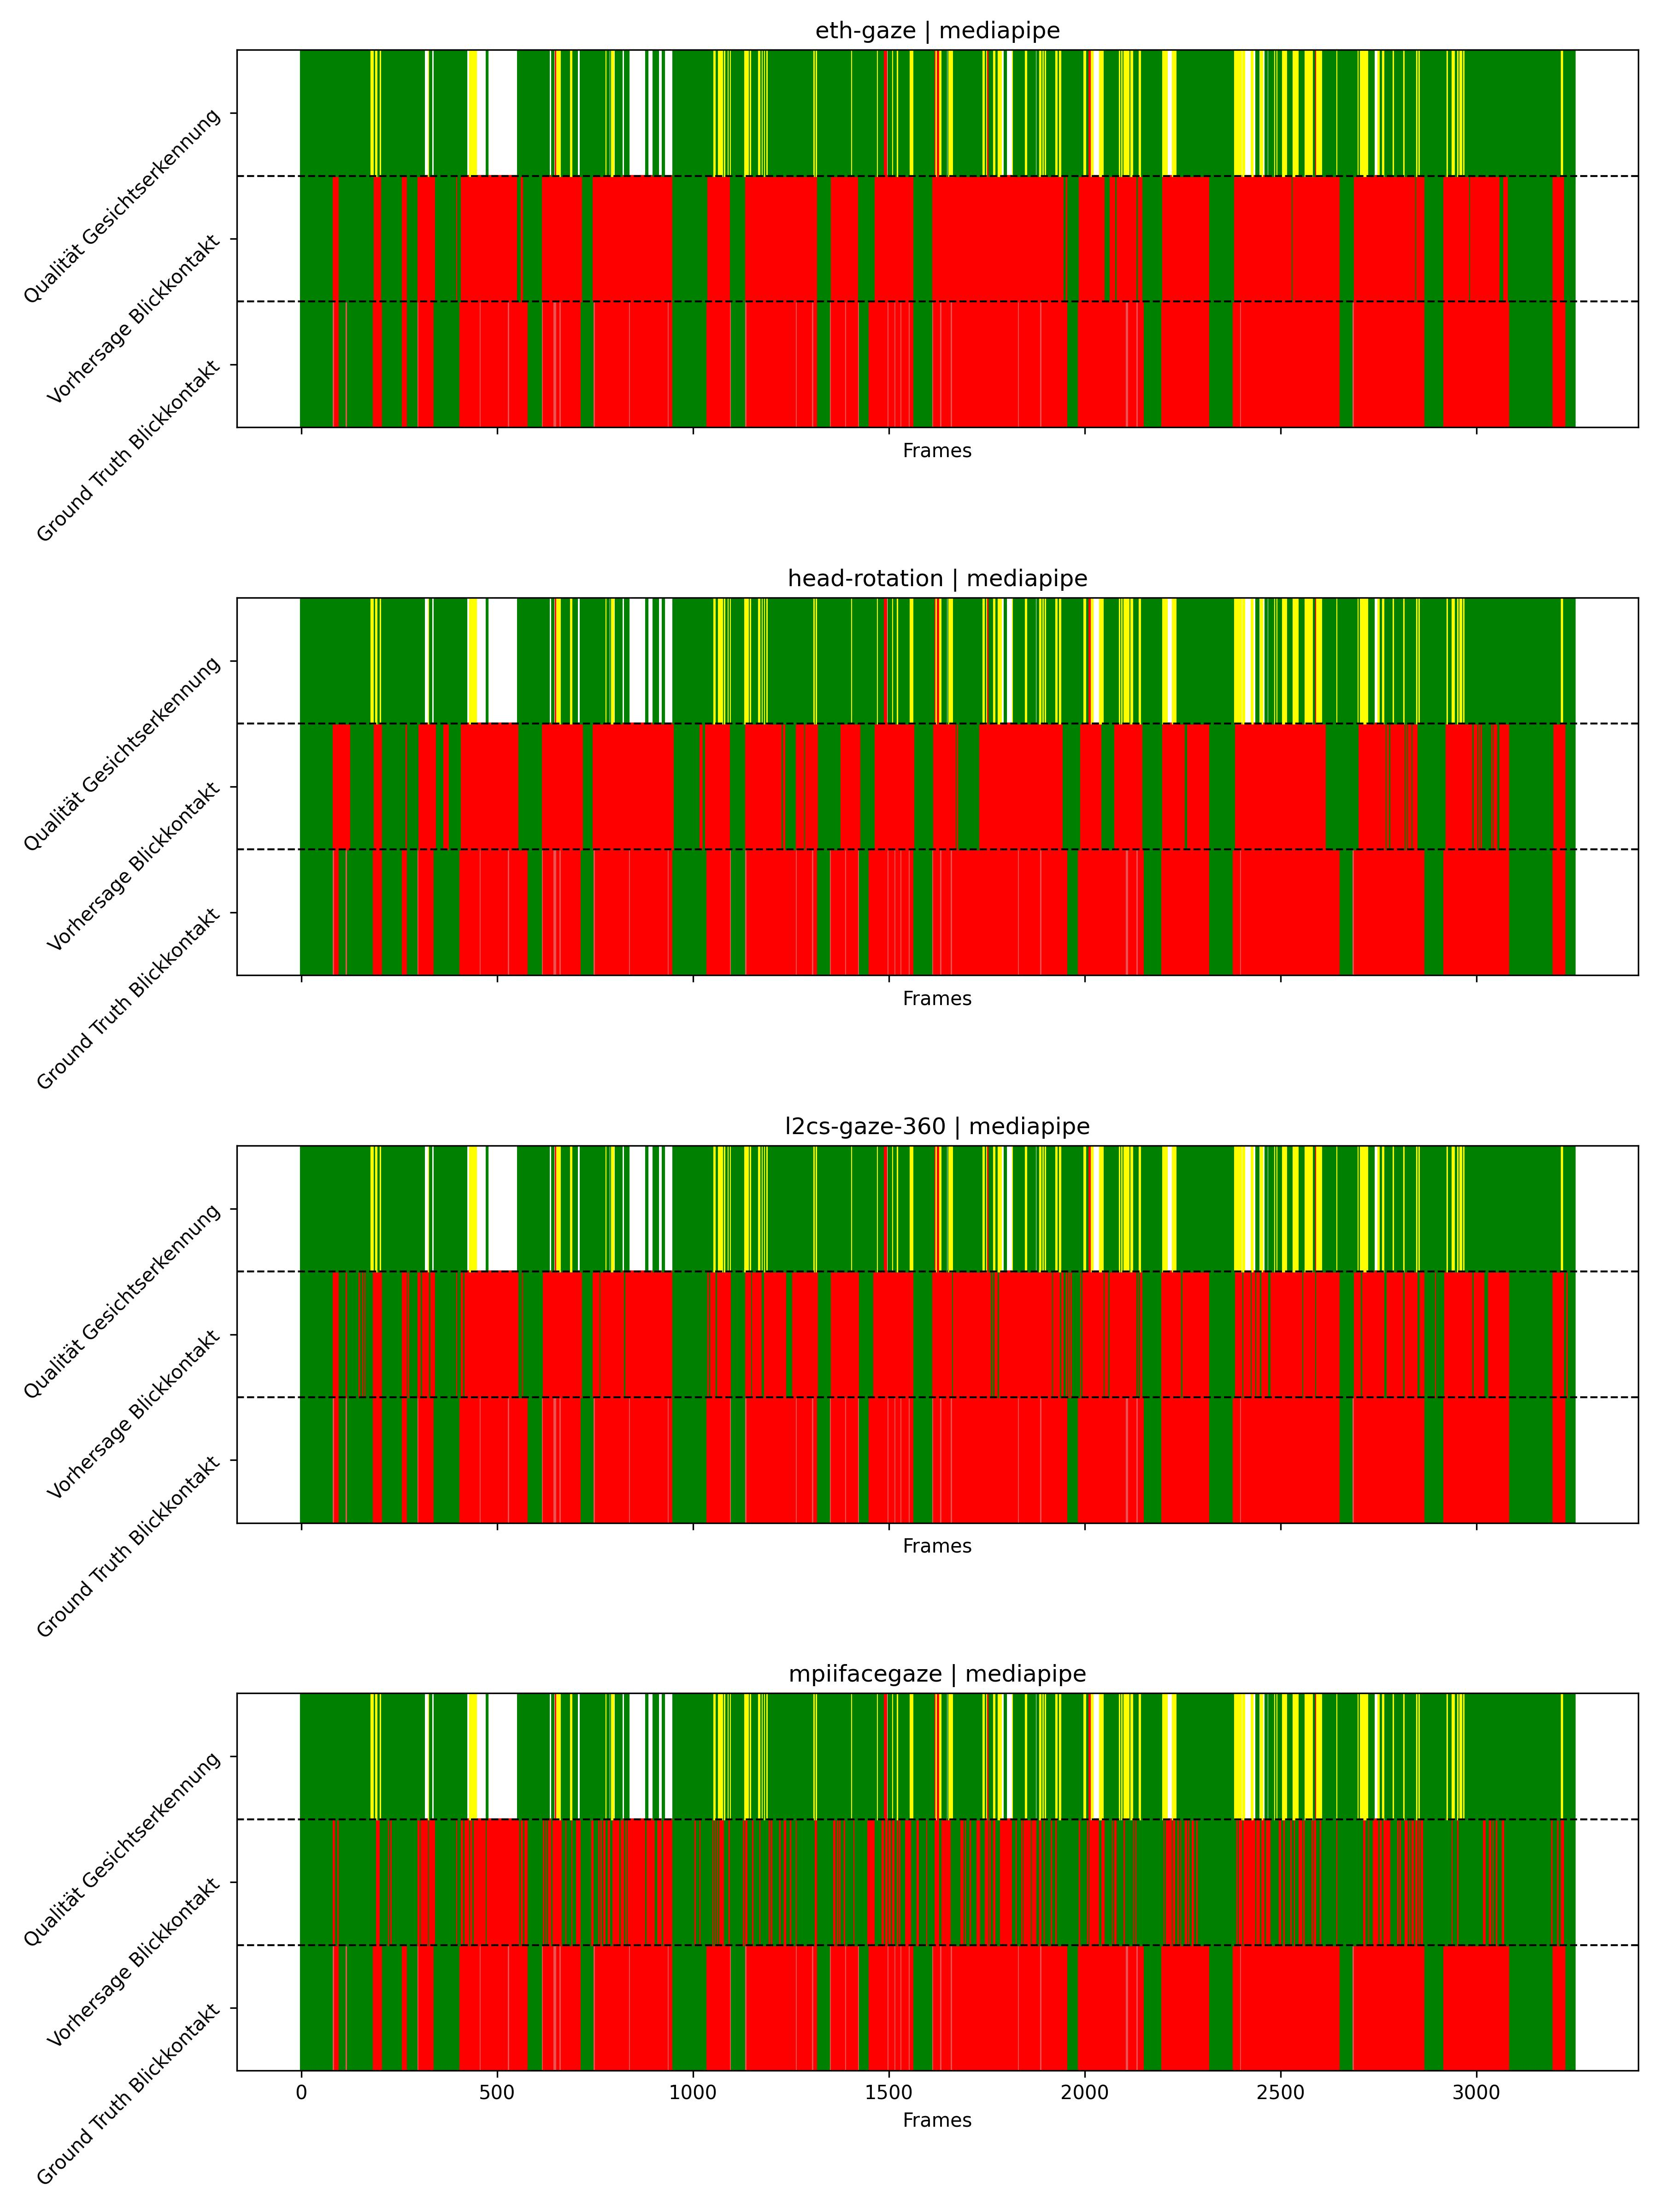
\includegraphics[width=1\linewidth]{appendix/20-mediapipe-overview-gaze.jpg}
\caption{Überblick über die Ground Truth des Blickkontakts, die Vorhersage des Blickkontakts und die Qualität der Gesichtserkennung mit \mediapipe. Die Bedeutung der Farben ist in Abbildung \ref{fig:evaluation:gaze:mpiifacegaze} erklärt.}
\end{figure}

\section{Video 21}
\begin{figure}[H]
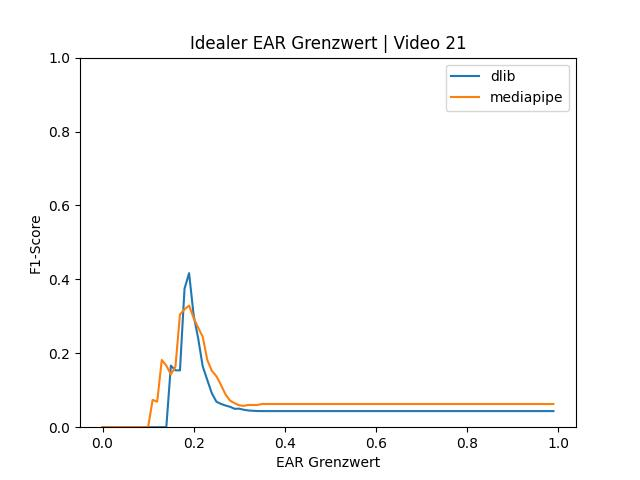
\includegraphics[width=0.7\linewidth]{appendix/21_f1-score-blink.jpg}
\caption{Ergebnisse der Bestimmung des idealen EAR-Grenzwerts für Video 21.}
\end{figure}

\begin{figure}[H]
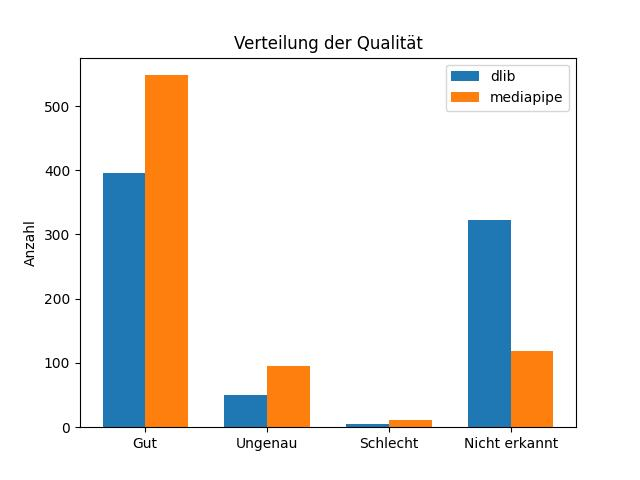
\includegraphics[width=0.7\linewidth]{appendix/21_bar-quality.jpg}
\caption{Aufteilung der Gesichtserkennungsqualität von Video 21.}
\end{figure}

\begin{table}[H]
\centering
\begin{tabular}{l|l|c c |c}
\toprule
\textbf{Gesichtserkennung} & \textbf{Blickrichtung} & \textbf{Seitenlänge} $\hitthresholdsize$ & \textbf{Verschiebung} $\hitthresholdposition$ & \textbf{F1-Score} \\ 
\midrule
\multirow{4}*{dlib}& ETH-XGaze & 0,214 & -0,002 & 0,951  \\ 
& Gaze360 & 0,5 & 0,035 & 0,896 \\ 
& MPIIFaceGaze & 0,082 & -0,039 & 0,872  \\ 
& Kopfrotation & 0,133 & 0,182 & 0,82  \\ 
\hline\multirow{4}*{MediaPipe}& ETH-XGaze & 0,255 & -0,027 & 0,964  \\ 
& Gaze360 & 0,49 & 0,035 & 0,858 \\ 
& MPIIFaceGaze & 0,061 & -0,039 & 0,739  \\ 
& Kopfrotation & 0,122 & 0,157 & 0,874  \\ 
\bottomrule\end{tabular}
\caption{Ergebnis des Hyperparameter-Tunings für die Zone speziell für Video 21.}
\label{tab:appendix:21:local}
\end{table}
\begin{table}[H]
\centering
\begin{tabular}{l|l|c c c c|c c|c}
\toprule
\textbf{Gesichtserkennung} & \textbf{Blickrichtung} & $TP$ & $TN$& $FP$ & $FN$ & \textbf{Precision} & \textbf{Recall} & \textbf{F1-Score} \\ 
\midrule
\multirow{4}*{dlib}& ETH-XGaze & 264 & 473 & 19 & 12 & 0,933 & 0,957 & 0,945 \\ 
& Gaze360 & 252 & 452 & 40 & 24 & 0,863 & 0,913 & 0,887 \\ 
& MPIIFaceGaze & 265 & 370 & 122 & 11 & 0,685 & 0,96 & 0,799 \\ 
& Kopfrotation & 261 & 353 & 139 & 15 & 0,652 & 0,946 & 0,772 \\ 
\hline\multirow{4}*{MediaPipe}& ETH-XGaze & 276 & 464 & 32 & 0 & 0,896 & 1,0 & 0,945 \\ 
& Gaze360 & 225 & 449 & 47 & 51 & 0,827 & 0,815 & 0,821 \\ 
& MPIIFaceGaze & 228 & 280 & 216 & 48 & 0,514 & 0,826 & 0,633 \\ 
& Kopfrotation & 274 & 340 & 156 & 2 & 0,637 & 0,993 & 0,776 \\ 
\bottomrule\end{tabular}
\caption{Zusammensetzung des F1-Scores unter Verwendung der in Kapitel \ref{sec:evaluation:results:gaze:threshold} bestimmten globalen Parameter $\hitthresholdsize$ und $\hitthresholdposition$.}
\label{tab:appendix:21:f1}
\end{table}
\begin{figure}[H]
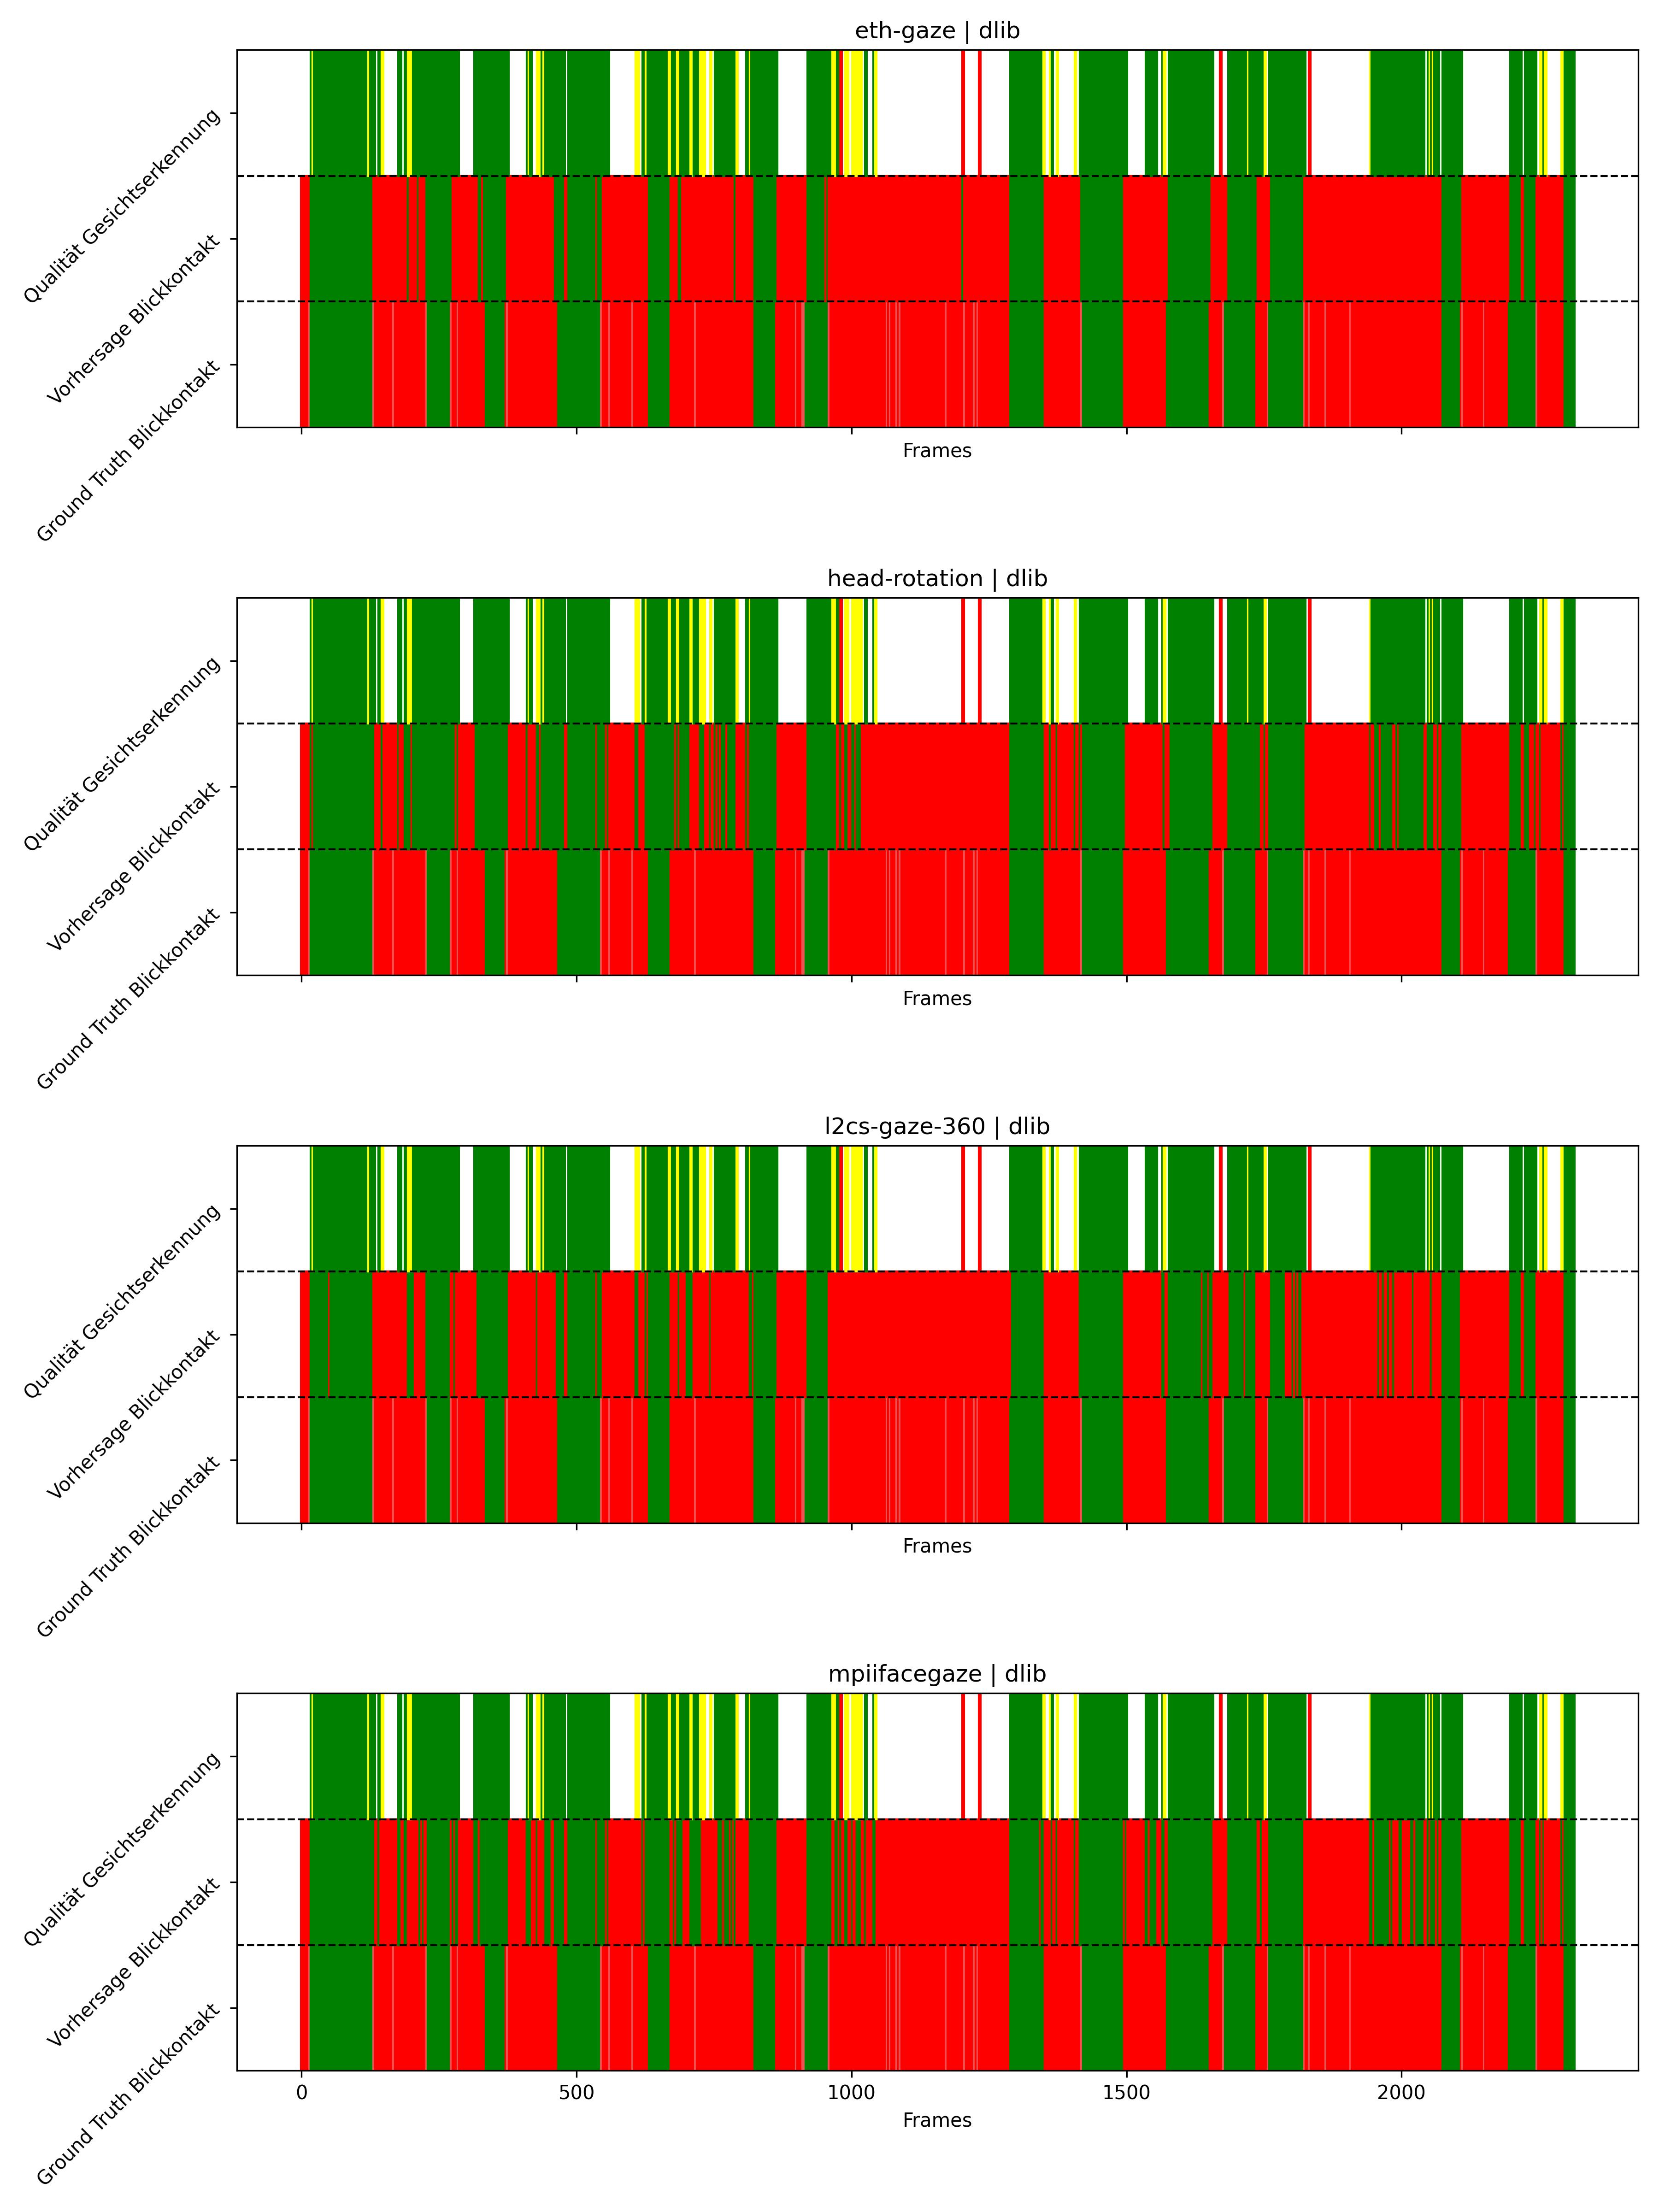
\includegraphics[width=1\linewidth]{appendix/21-dlib-overview-gaze.jpg}
\caption{Überblick über die Ground Truth des Blickkontakts, die Vorhersage des Blickkontakts und die Qualität der Gesichtserkennung mit \dlib. Die Bedeutung der Farben ist in Abbildung \ref{fig:evaluation:gaze:mpiifacegaze} erklärt.  }
\end{figure}

\begin{figure}[H]
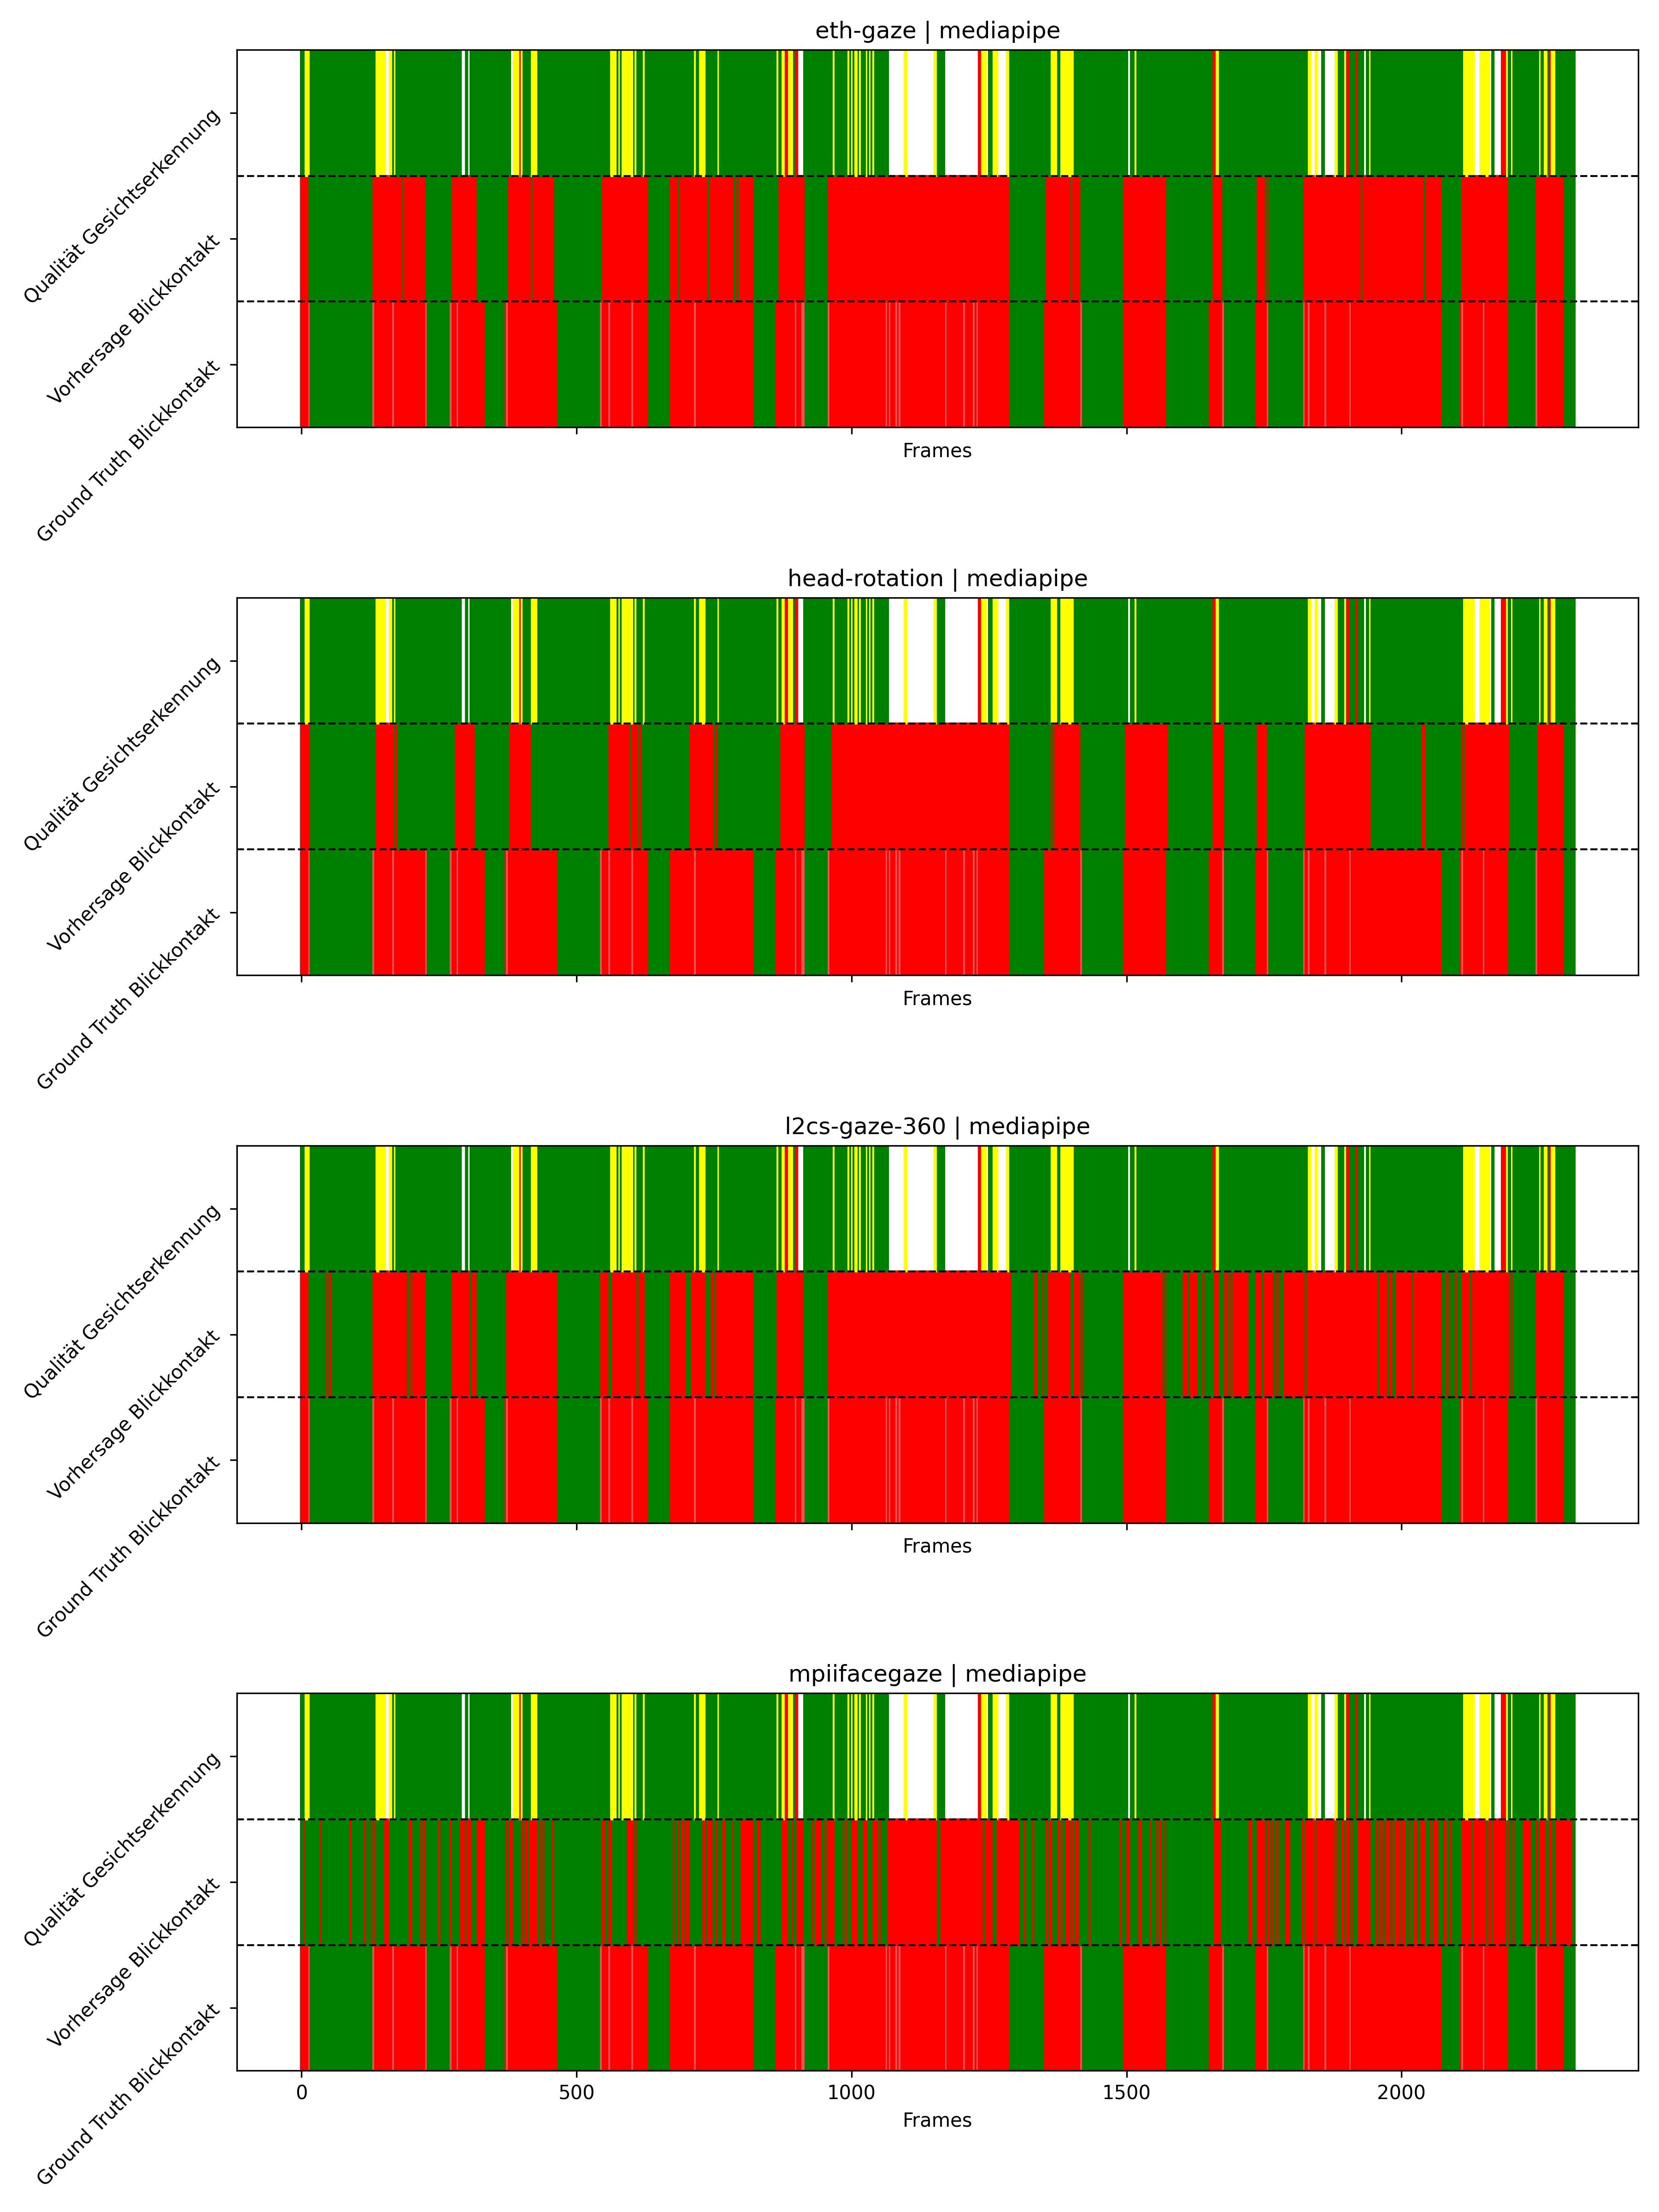
\includegraphics[width=1\linewidth]{appendix/21-mediapipe-overview-gaze.jpg}
\caption{Überblick über die Ground Truth des Blickkontakts, die Vorhersage des Blickkontakts und die Qualität der Gesichtserkennung mit \mediapipe. Die Bedeutung der Farben ist in Abbildung \ref{fig:evaluation:gaze:mpiifacegaze} erklärt.}
\end{figure}

\section{Video 22}
\begin{figure}[H]
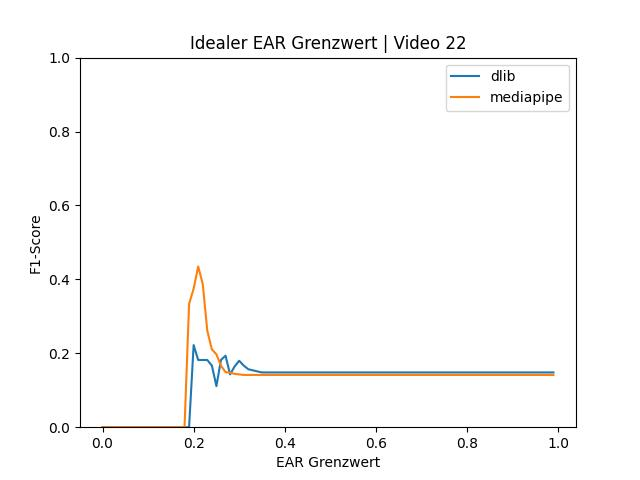
\includegraphics[width=0.7\linewidth]{appendix/22_f1-score-blink.jpg}
\caption{Ergebnisse der Bestimmung des idealen EAR-Grenzwerts für Video 22.}
\end{figure}

\begin{figure}[H]
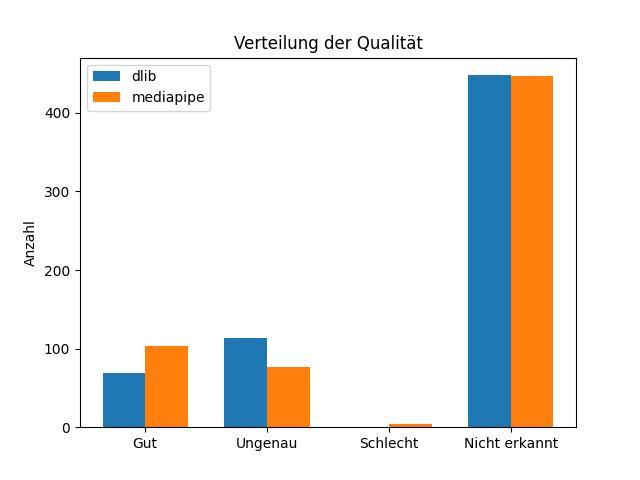
\includegraphics[width=0.7\linewidth]{appendix/22_bar-quality.jpg}
\caption{Aufteilung der Gesichtserkennungsqualität von Video 22.}
\end{figure}

\begin{table}[H]
\centering
\begin{tabular}{l|l|c c |c}
\toprule
\textbf{Gesichtserkennung} & \textbf{Blickrichtung} & \textbf{Seitenlänge} $\hitthresholdsize$ & \textbf{Verschiebung} $\hitthresholdposition$ & \textbf{F1-Score} \\ 
\midrule
\multirow{4}*{dlib}& ETH-XGaze & 0,337 & 0,059 & 0,569  \\ 
& Gaze360 & 0 & 0 & 0 \\ 
& MPIIFaceGaze & 0,112 & 0,059 & 0,51  \\ 
& Kopfrotation & 0,286 & 0,157 & 0,528  \\ 
\hline\multirow{4}*{MediaPipe}& ETH-XGaze & 0,388 & 0,071 & 0,576  \\ 
& Gaze360 & 0 & 0 & 0 \\ 
& MPIIFaceGaze & 0,112 & 0,059 & 0,527  \\ 
& Kopfrotation & 0,245 & 0,133 & 0,625  \\ 
\bottomrule\end{tabular}
\caption{Ergebnis des Hyperparameter-Tunings für die Zone speziell für Video 22.}
\label{tab:appendix:22:local}
\end{table}
\begin{table}[H]
\centering
\begin{tabular}{l|l|c c c c|c c|c}
\toprule
\textbf{Gesichtserkennung} & \textbf{Blickrichtung} & $TP$ & $TN$& $FP$ & $FN$ & \textbf{Precision} & \textbf{Recall} & \textbf{F1-Score} \\ 
\midrule
\multirow{4}*{dlib}& ETH-XGaze & 58 & 462 & 17 & 94 & 0,773 & 0,382 & 0,511 \\ 
& Gaze360 & 0 & 478 & 1 & 152 & 0,0 & 0,0 & 0,0 \\ 
& MPIIFaceGaze & 66 & 390 & 89 & 86 & 0,426 & 0,434 & 0,43 \\ 
& Kopfrotation & 79 & 393 & 86 & 73 & 0,479 & 0,52 & 0,498 \\ 
\hline\multirow{4}*{MediaPipe}& ETH-XGaze & 51 & 462 & 17 & 101 & 0,75 & 0,336 & 0,464 \\ 
& Gaze360 & 0 & 479 & 0 & 152 & 0 & 0,0 & 0,0 \\ 
& MPIIFaceGaze & 49 & 406 & 73 & 103 & 0,402 & 0,322 & 0,358 \\ 
& Kopfrotation & 83 & 434 & 45 & 69 & 0,648 & 0,546 & 0,593 \\ 
\bottomrule\end{tabular}
\caption{Zusammensetzung des F1-Scores unter Verwendung der in Kapitel \ref{sec:evaluation:results:gaze:threshold} bestimmten globalen Parameter $\hitthresholdsize$ und $\hitthresholdposition$.}
\label{tab:appendix:22:f1}
\end{table}
\begin{figure}[H]
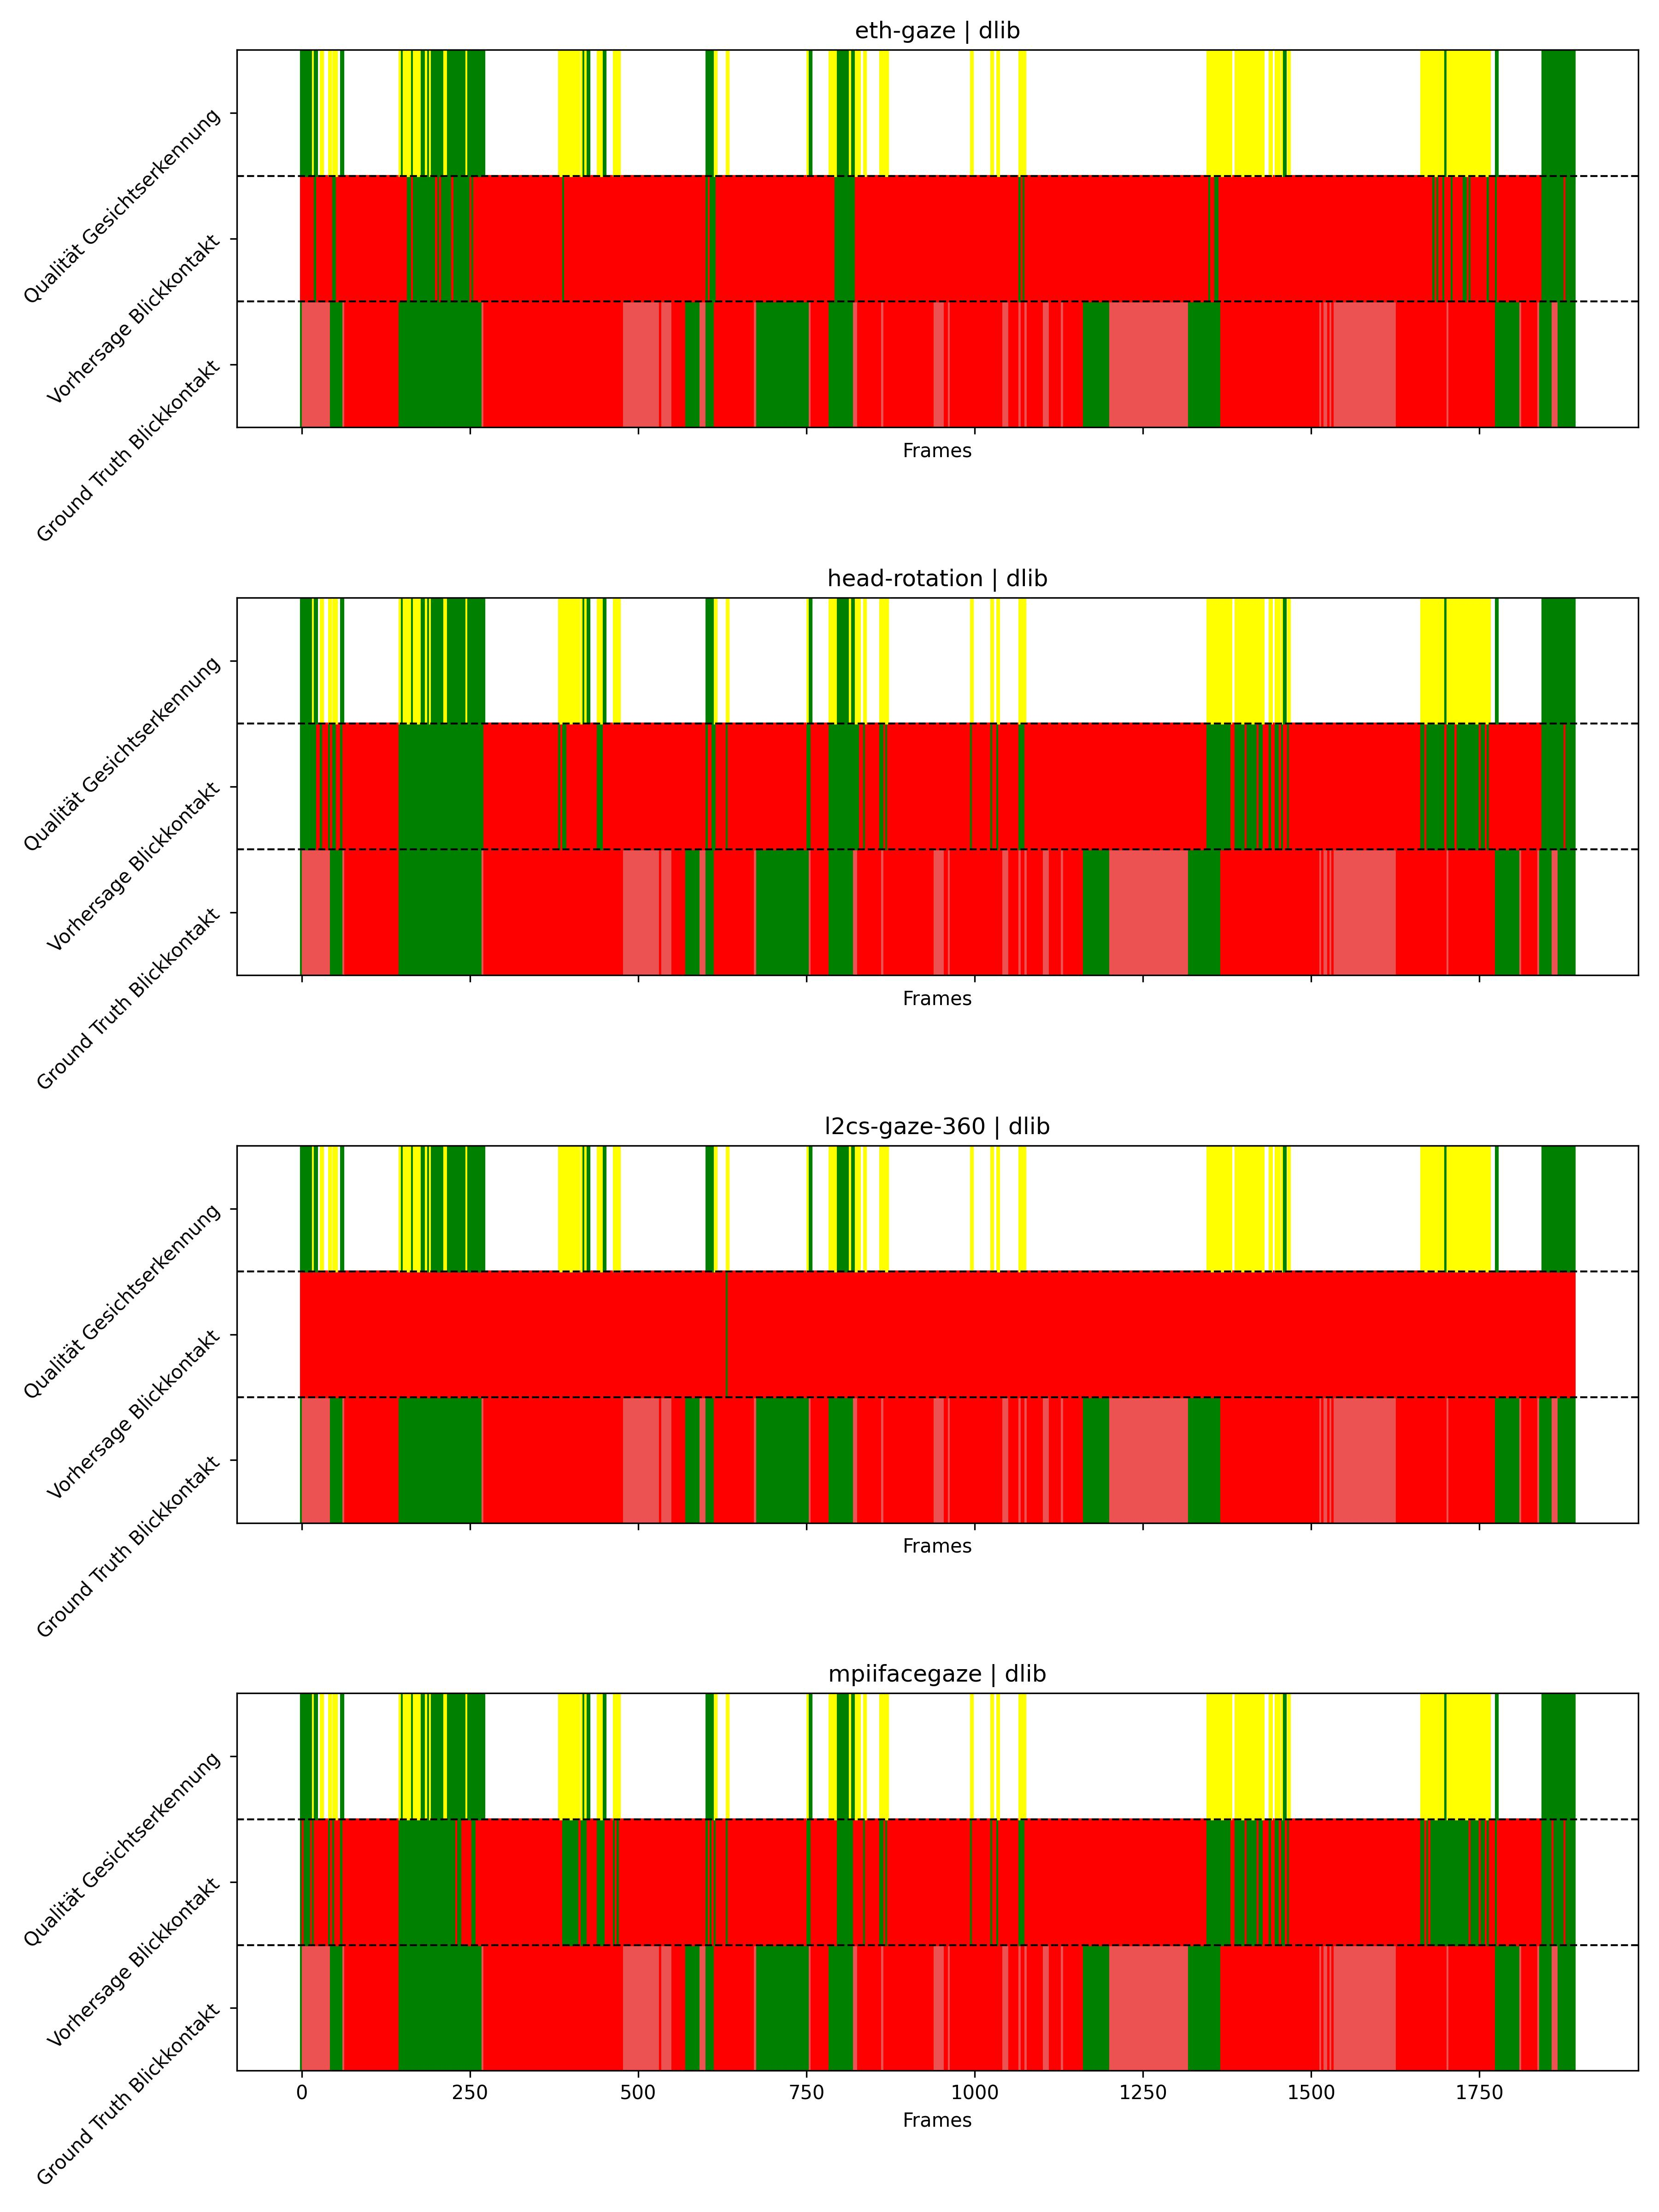
\includegraphics[width=1\linewidth]{appendix/22-dlib-overview-gaze.jpg}
\caption{Überblick über die Ground Truth des Blickkontakts, die Vorhersage des Blickkontakts und die Qualität der Gesichtserkennung mit \dlib. Die Bedeutung der Farben ist in Abbildung \ref{fig:evaluation:gaze:mpiifacegaze} erklärt.  }
\end{figure}

\begin{figure}[H]
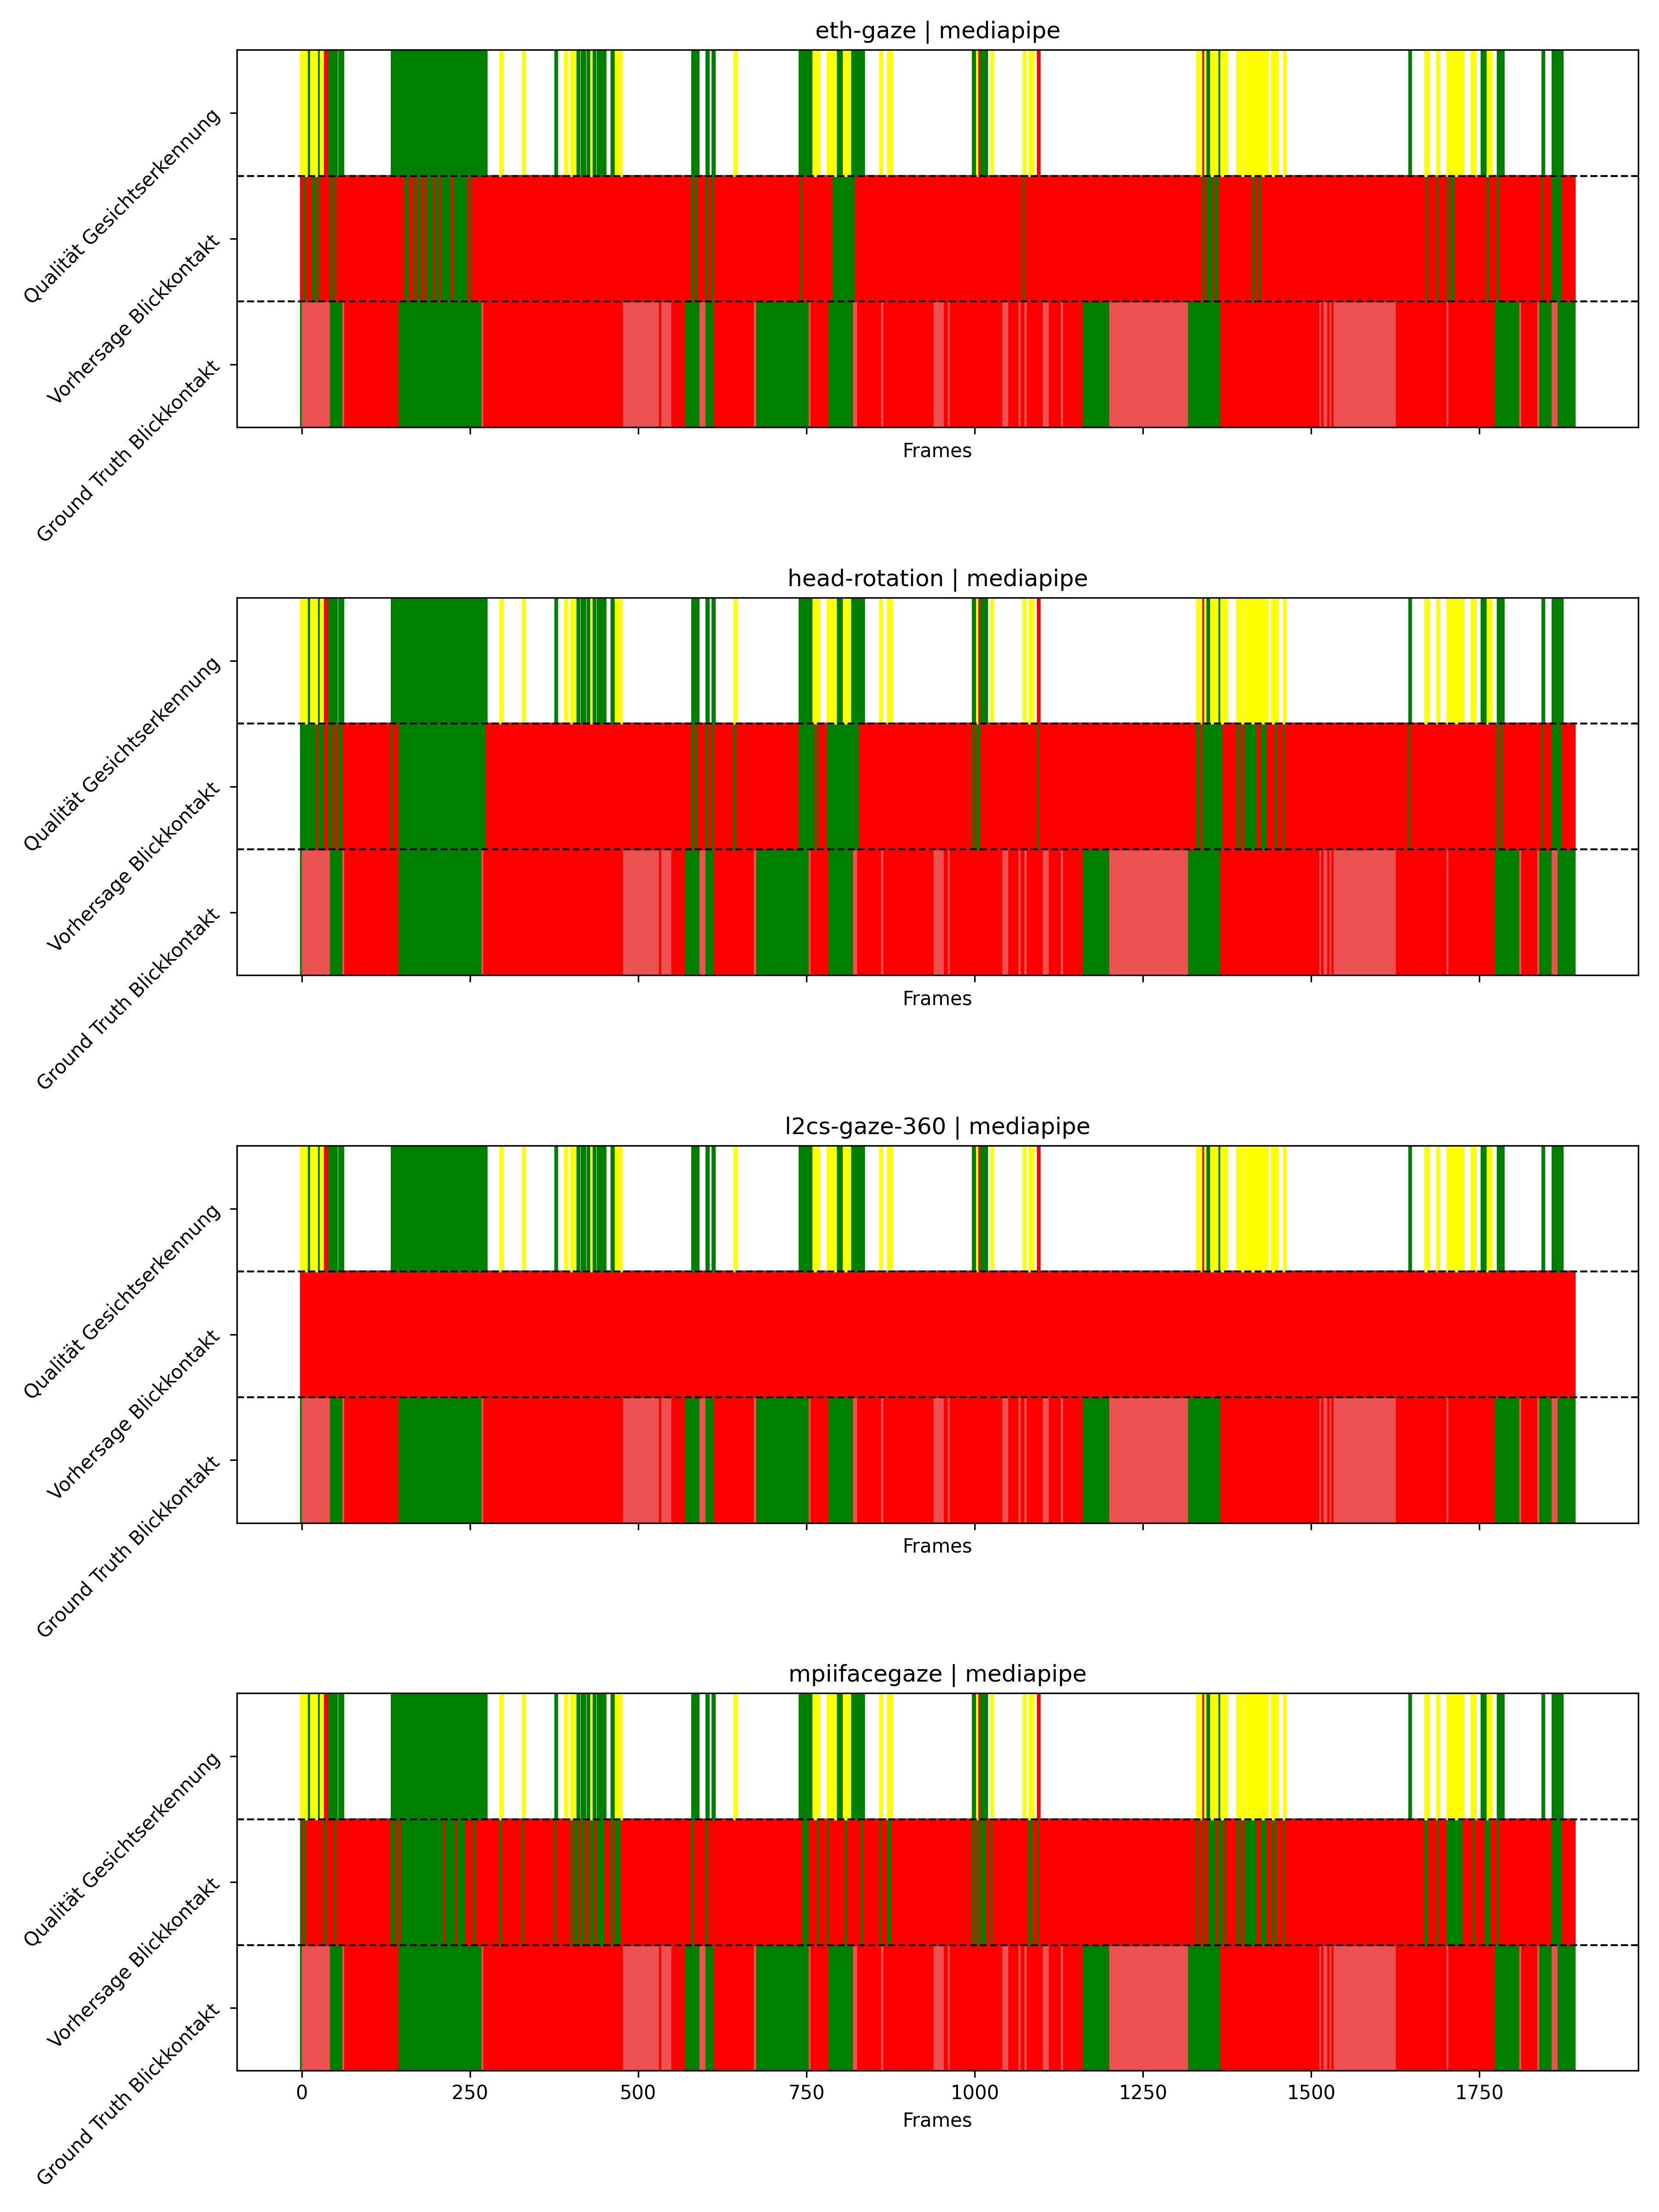
\includegraphics[width=1\linewidth]{appendix/22-mediapipe-overview-gaze.jpg}
\caption{Überblick über die Ground Truth des Blickkontakts, die Vorhersage des Blickkontakts und die Qualität der Gesichtserkennung mit \mediapipe. Die Bedeutung der Farben ist in Abbildung \ref{fig:evaluation:gaze:mpiifacegaze} erklärt.}
\end{figure}

\section{Video 23}
\begin{figure}[H]
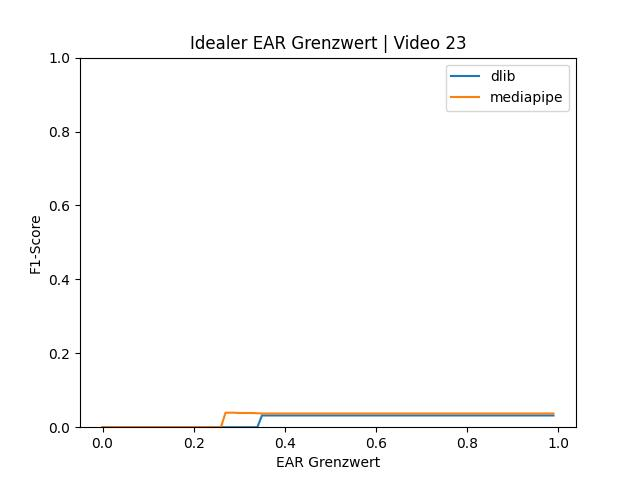
\includegraphics[width=0.7\linewidth]{appendix/23_f1-score-blink.jpg}
\caption{Ergebnisse der Bestimmung des idealen EAR-Grenzwerts für Video 23.}
\end{figure}

\begin{figure}[H]
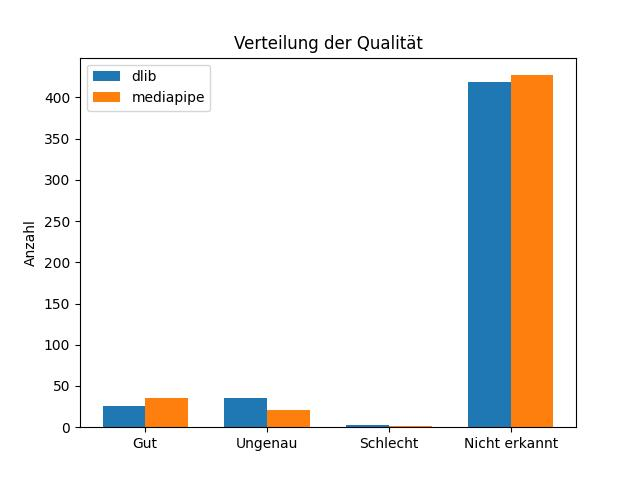
\includegraphics[width=0.7\linewidth]{appendix/23_bar-quality.jpg}
\caption{Aufteilung der Gesichtserkennungsqualität von Video 23.}
\end{figure}

\begin{table}[H]
\centering
\begin{tabular}{l|l|c c |c}
\toprule
\textbf{Gesichtserkennung} & \textbf{Blickrichtung} & \textbf{Seitenlänge} $\hitthresholdsize$ & \textbf{Verschiebung} $\hitthresholdposition$ & \textbf{F1-Score} \\ 
\midrule
\multirow{4}*{dlib}& ETH-XGaze & 0,276 & 0,035 & 0,81  \\ 
& Gaze360 & 0,112 & -0,014 & 0,049 \\ 
& MPIIFaceGaze & 0,163 & 0,12 & 0,783  \\ 
& Kopfrotation & 0,276 & 0,231 & 0,686  \\ 
\hline\multirow{4}*{MediaPipe}& ETH-XGaze & 0,255 & 0,047 & 0,843  \\ 
& Gaze360 & 0,408 & 0,047 & 0,385 \\ 
& MPIIFaceGaze & 0,092 & 0,047 & 0,864  \\ 
& Kopfrotation & 0,122 & 0,243 & 0,864  \\ 
\bottomrule\end{tabular}
\caption{Ergebnis des Hyperparameter-Tunings für die Zone speziell für Video 23.}
\label{tab:appendix:23:local}
\end{table}
\begin{table}[H]
\centering
\begin{tabular}{l|l|c c c c|c c|c}
\toprule
\textbf{Gesichtserkennung} & \textbf{Blickrichtung} & $TP$ & $TN$& $FP$ & $FN$ & \textbf{Precision} & \textbf{Recall} & \textbf{F1-Score} \\ 
\midrule
\multirow{4}*{dlib}& ETH-XGaze & 28 & 436 & 8 & 12 & 0,778 & 0,7 & 0,737 \\ 
& Gaze360 & 1 & 443 & 1 & 39 & 0,5 & 0,025 & 0,048 \\ 
& MPIIFaceGaze & 18 & 420 & 24 & 22 & 0,429 & 0,45 & 0,439 \\ 
& Kopfrotation & 32 & 415 & 29 & 8 & 0,525 & 0,8 & 0,634 \\ 
\hline\multirow{4}*{MediaPipe}& ETH-XGaze & 31 & 439 & 5 & 9 & 0,861 & 0,775 & 0,816 \\ 
& Gaze360 & 9 & 442 & 2 & 31 & 0,818 & 0,225 & 0,353 \\ 
& MPIIFaceGaze & 16 & 427 & 17 & 24 & 0,485 & 0,4 & 0,438 \\ 
& Kopfrotation & 33 & 437 & 7 & 7 & 0,825 & 0,825 & 0,825 \\ 
\bottomrule\end{tabular}
\caption{Zusammensetzung des F1-Scores unter Verwendung der in Kapitel \ref{sec:evaluation:results:gaze:threshold} bestimmten globalen Parameter $\hitthresholdsize$ und $\hitthresholdposition$.}
\label{tab:appendix:23:f1}
\end{table}
\begin{figure}[H]
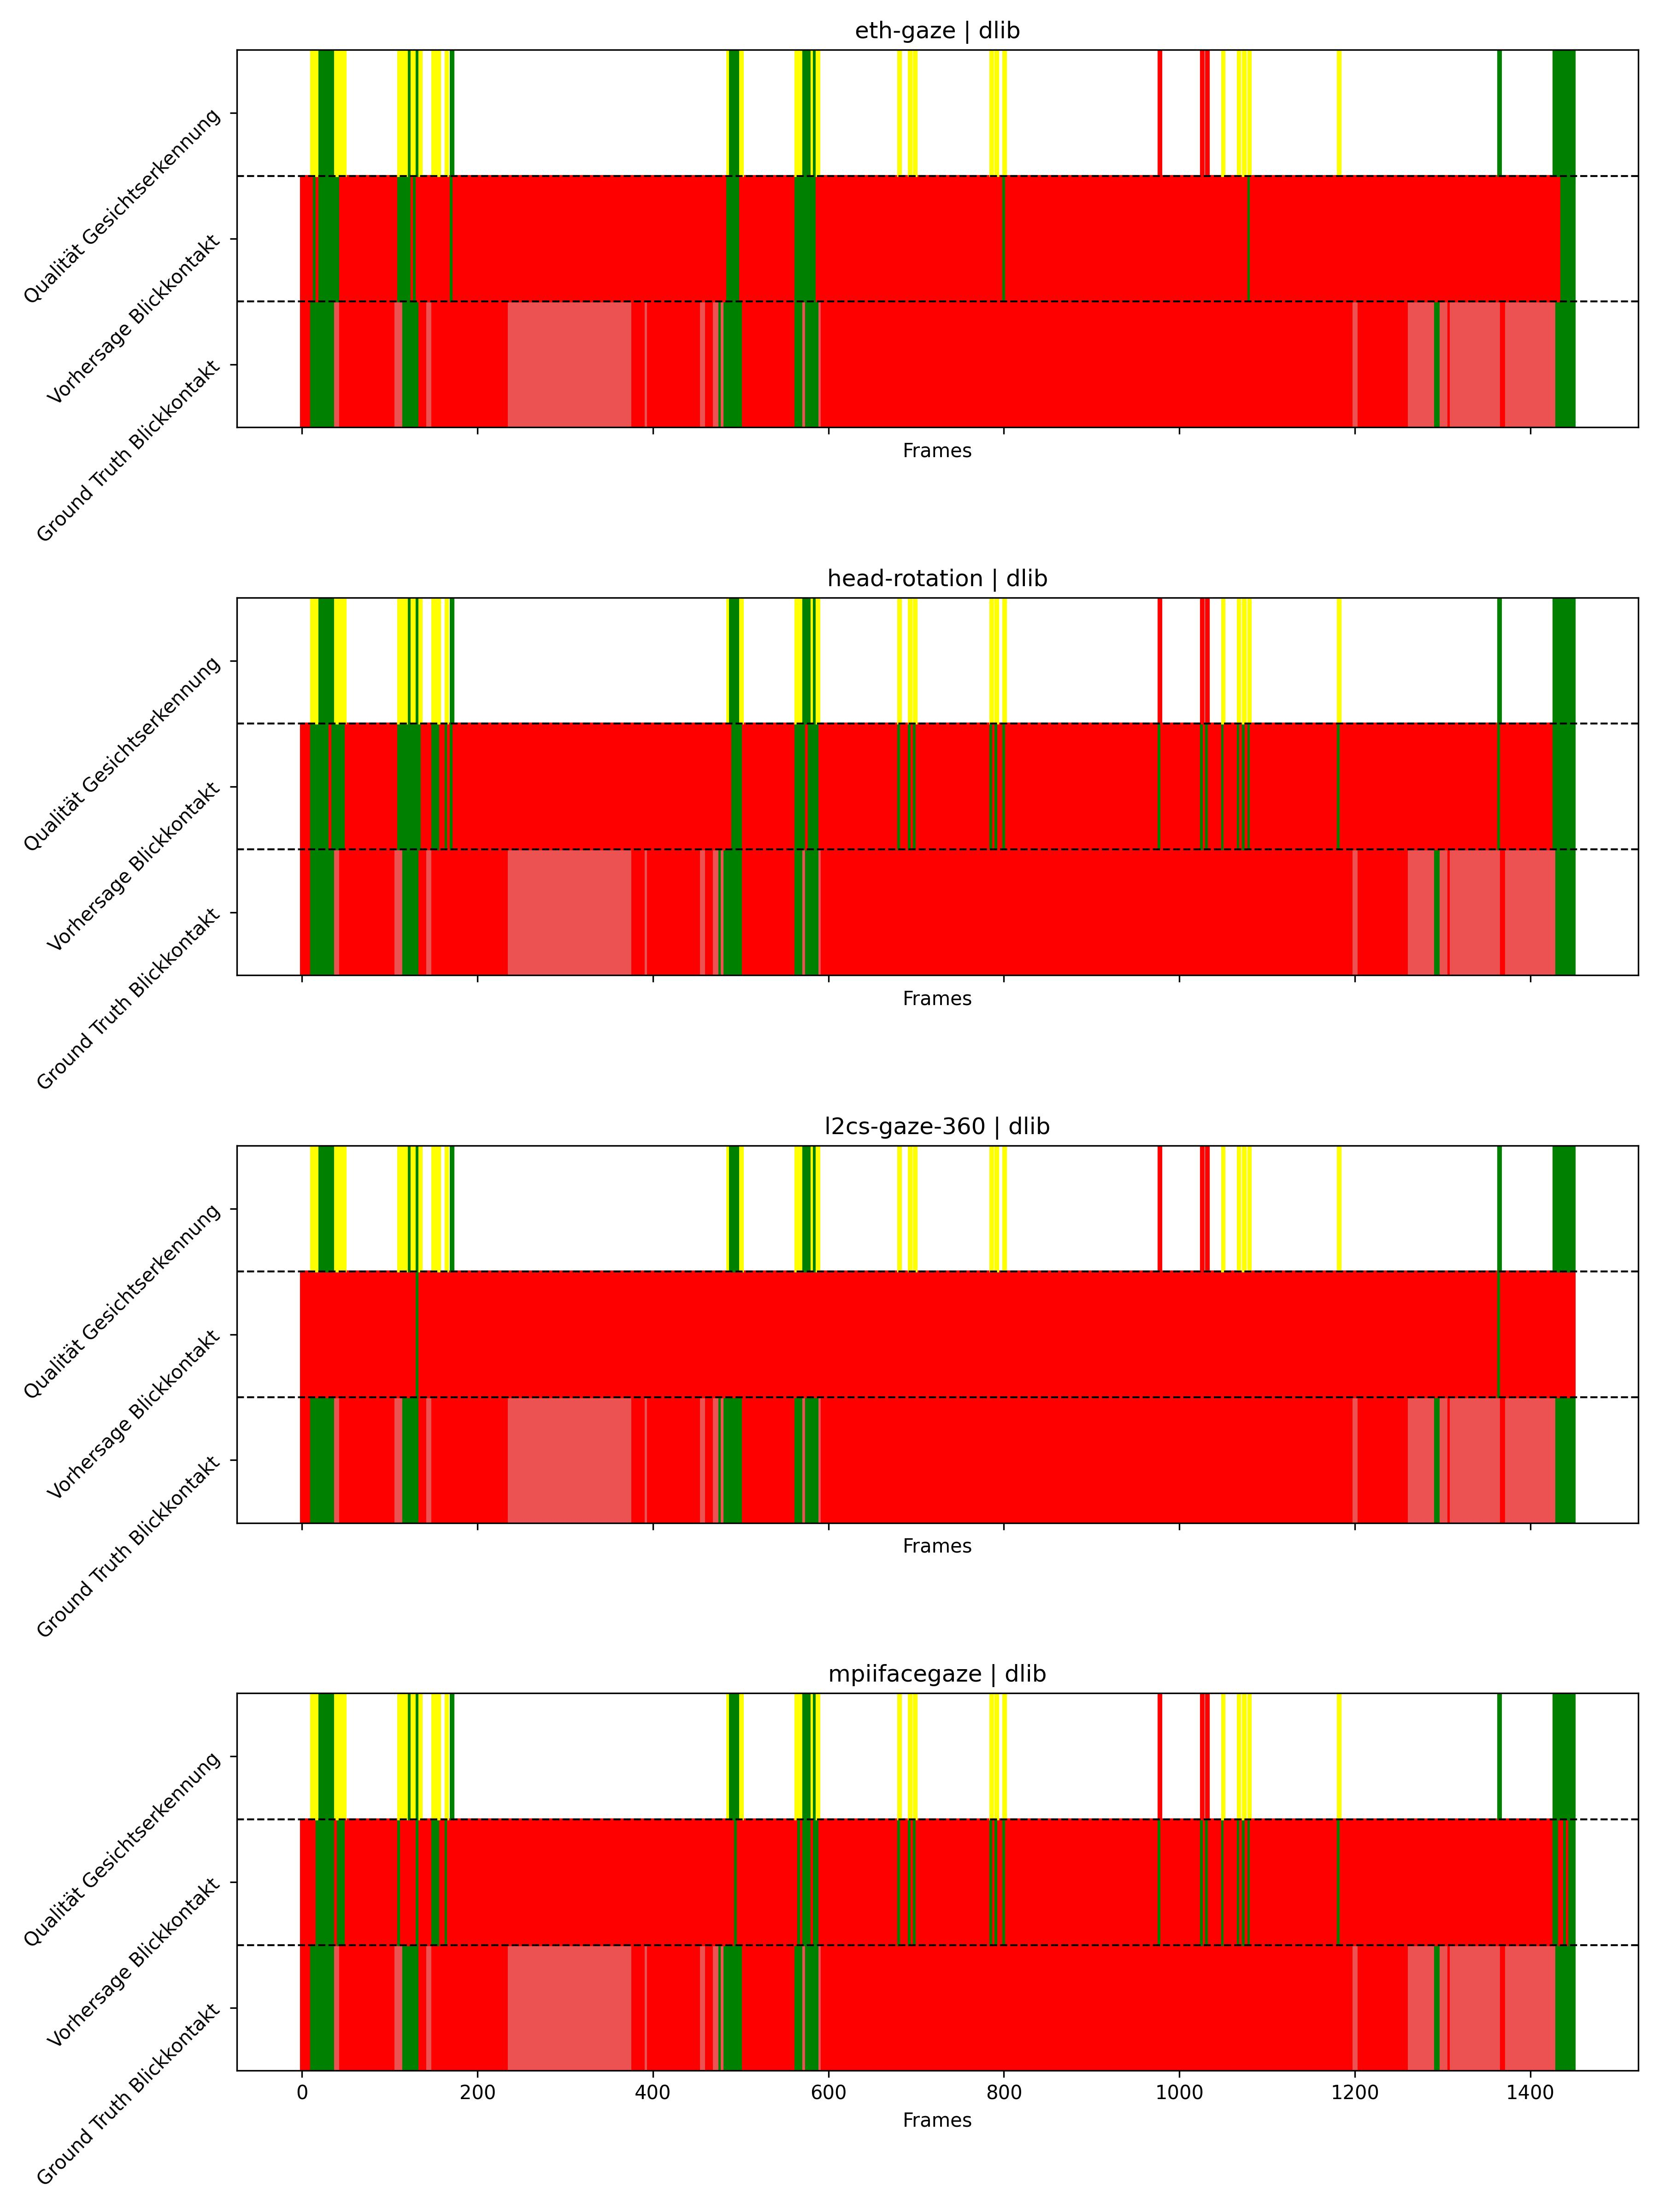
\includegraphics[width=1\linewidth]{appendix/23-dlib-overview-gaze.jpg}
\caption{Überblick über die Ground Truth des Blickkontakts, die Vorhersage des Blickkontakts und die Qualität der Gesichtserkennung mit \dlib. Die Bedeutung der Farben ist in Abbildung \ref{fig:evaluation:gaze:mpiifacegaze} erklärt.  }
\end{figure}

\begin{figure}[H]
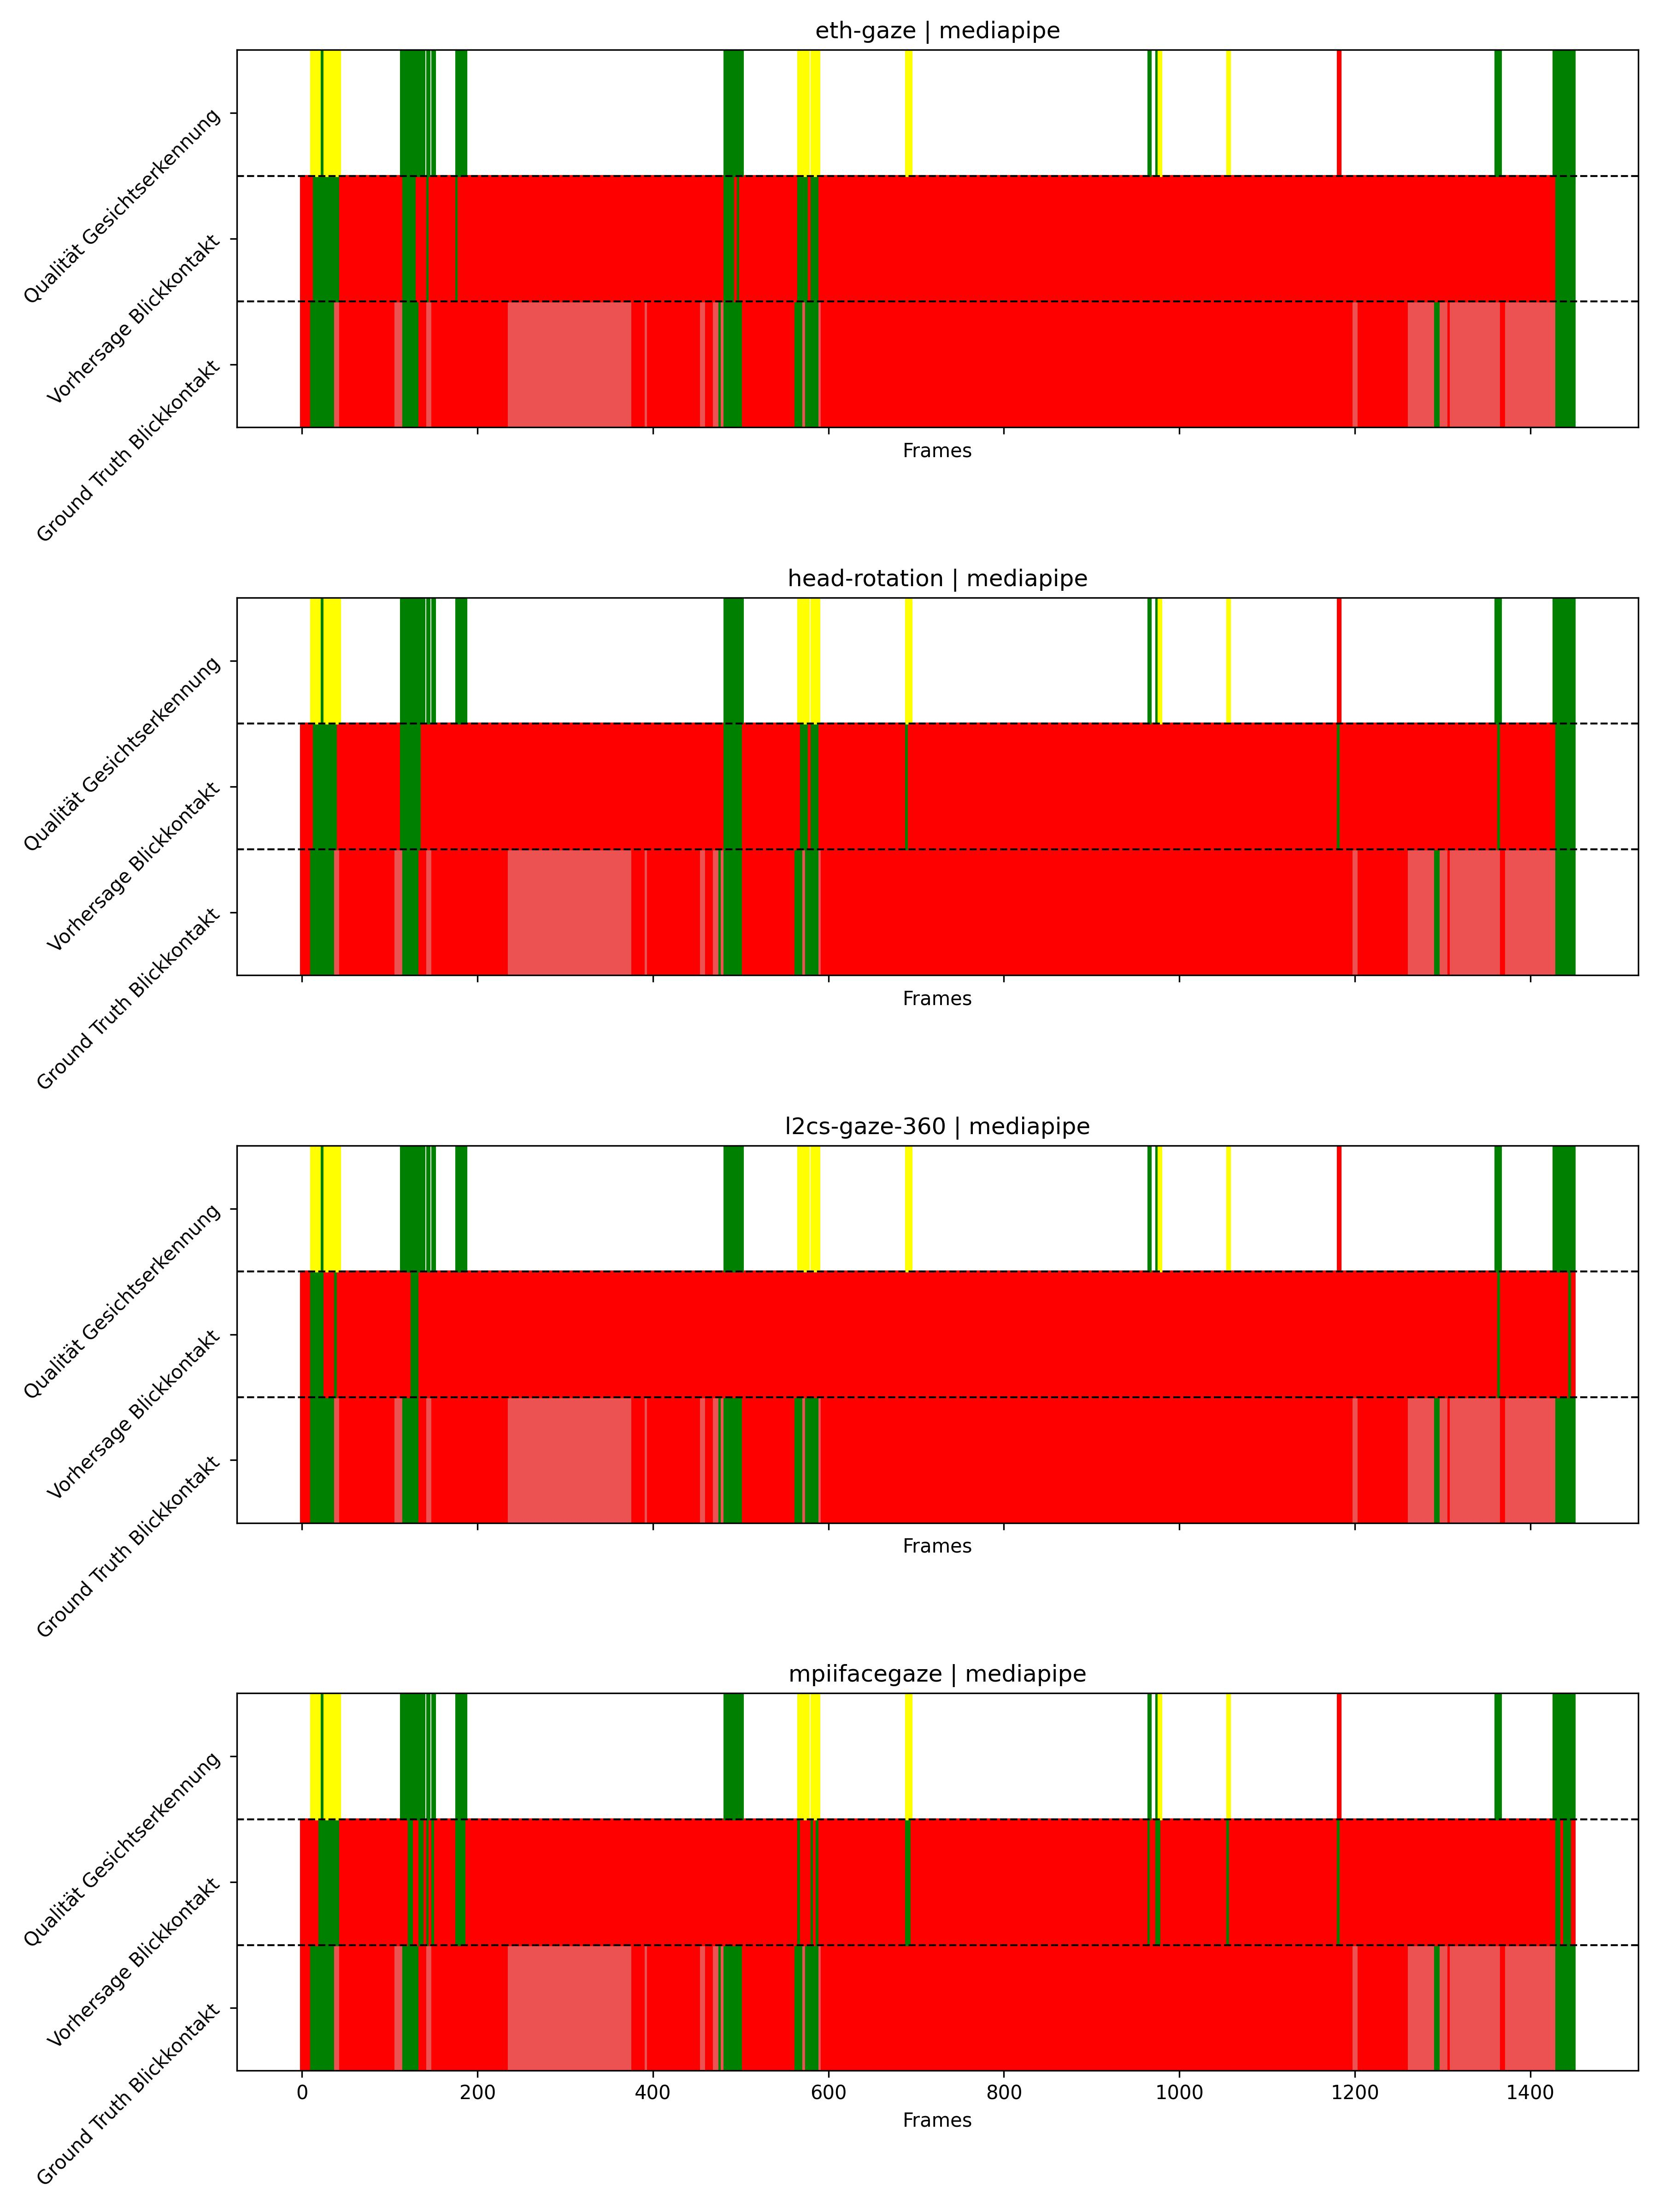
\includegraphics[width=1\linewidth]{appendix/23-mediapipe-overview-gaze.jpg}
\caption{Überblick über die Ground Truth des Blickkontakts, die Vorhersage des Blickkontakts und die Qualität der Gesichtserkennung mit \mediapipe. Die Bedeutung der Farben ist in Abbildung \ref{fig:evaluation:gaze:mpiifacegaze} erklärt.}
\end{figure}

\section{Video 24}
\begin{figure}[H]
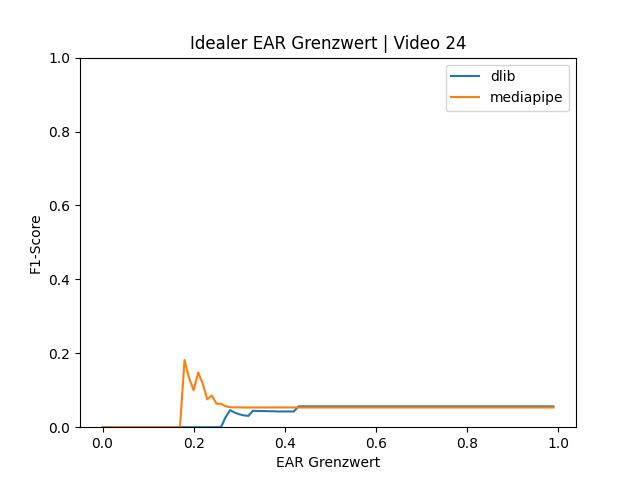
\includegraphics[width=0.7\linewidth]{appendix/24_f1-score-blink.jpg}
\caption{Ergebnisse der Bestimmung des idealen EAR-Grenzwerts für Video 24.}
\end{figure}

\begin{figure}[H]
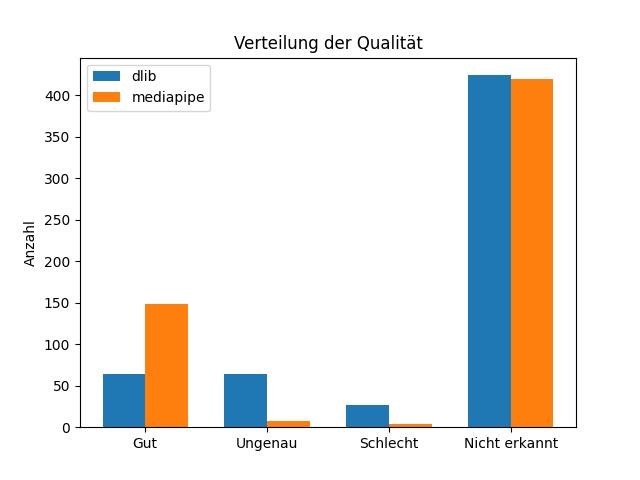
\includegraphics[width=0.7\linewidth]{appendix/24_bar-quality.jpg}
\caption{Aufteilung der Gesichtserkennungsqualität von Video 24.}
\end{figure}

\begin{table}[H]
\centering
\begin{tabular}{l|l|c c |c}
\toprule
\textbf{Gesichtserkennung} & \textbf{Blickrichtung} & \textbf{Seitenlänge} $\hitthresholdsize$ & \textbf{Verschiebung} $\hitthresholdposition$ & \textbf{F1-Score} \\ 
\midrule
\multirow{4}*{dlib}& ETH-XGaze & 0,418 & 0,071 & 0,899  \\ 
& Gaze360 & 0,5 & 0,047 & 0,782 \\ 
& MPIIFaceGaze & 0,122 & 0,071 & 0,8  \\ 
& Kopfrotation & 0,255 & 0,206 & 0,817  \\ 
\hline\multirow{4}*{MediaPipe}& ETH-XGaze & 0,449 & 0,047 & 0,839  \\ 
& Gaze360 & 0,5 & 0,035 & 0,601 \\ 
& MPIIFaceGaze & 0,092 & 0,047 & 0,759  \\ 
& Kopfrotation & 0,122 & 0,218 & 0,834  \\ 
\bottomrule\end{tabular}
\caption{Ergebnis des Hyperparameter-Tunings für die Zone speziell für Video 24.}
\label{tab:appendix:24:local}
\end{table}
\begin{table}[H]
\centering
\begin{tabular}{l|l|c c c c|c c|c}
\toprule
\textbf{Gesichtserkennung} & \textbf{Blickrichtung} & $TP$ & $TN$& $FP$ & $FN$ & \textbf{Precision} & \textbf{Recall} & \textbf{F1-Score} \\ 
\midrule
\multirow{4}*{dlib}& ETH-XGaze & 92 & 455 & 10 & 22 & 0,902 & 0,807 & 0,852 \\ 
& Gaze360 & 77 & 459 & 6 & 37 & 0,928 & 0,675 & 0,782 \\ 
& MPIIFaceGaze & 62 & 429 & 36 & 52 & 0,633 & 0,544 & 0,585 \\ 
& Kopfrotation & 107 & 424 & 41 & 7 & 0,723 & 0,939 & 0,817 \\ 
\hline\multirow{4}*{MediaPipe}& ETH-XGaze & 83 & 455 & 10 & 31 & 0,892 & 0,728 & 0,802 \\ 
& Gaze360 & 49 & 459 & 6 & 65 & 0,891 & 0,43 & 0,58 \\ 
& MPIIFaceGaze & 45 & 421 & 44 & 69 & 0,506 & 0,395 & 0,443 \\ 
& Kopfrotation & 88 & 453 & 12 & 26 & 0,88 & 0,772 & 0,822 \\ 
\bottomrule\end{tabular}
\caption{Zusammensetzung des F1-Scores unter Verwendung der in Kapitel \ref{sec:evaluation:results:gaze:threshold} bestimmten globalen Parameter $\hitthresholdsize$ und $\hitthresholdposition$.}
\label{tab:appendix:24:f1}
\end{table}
\begin{figure}[H]
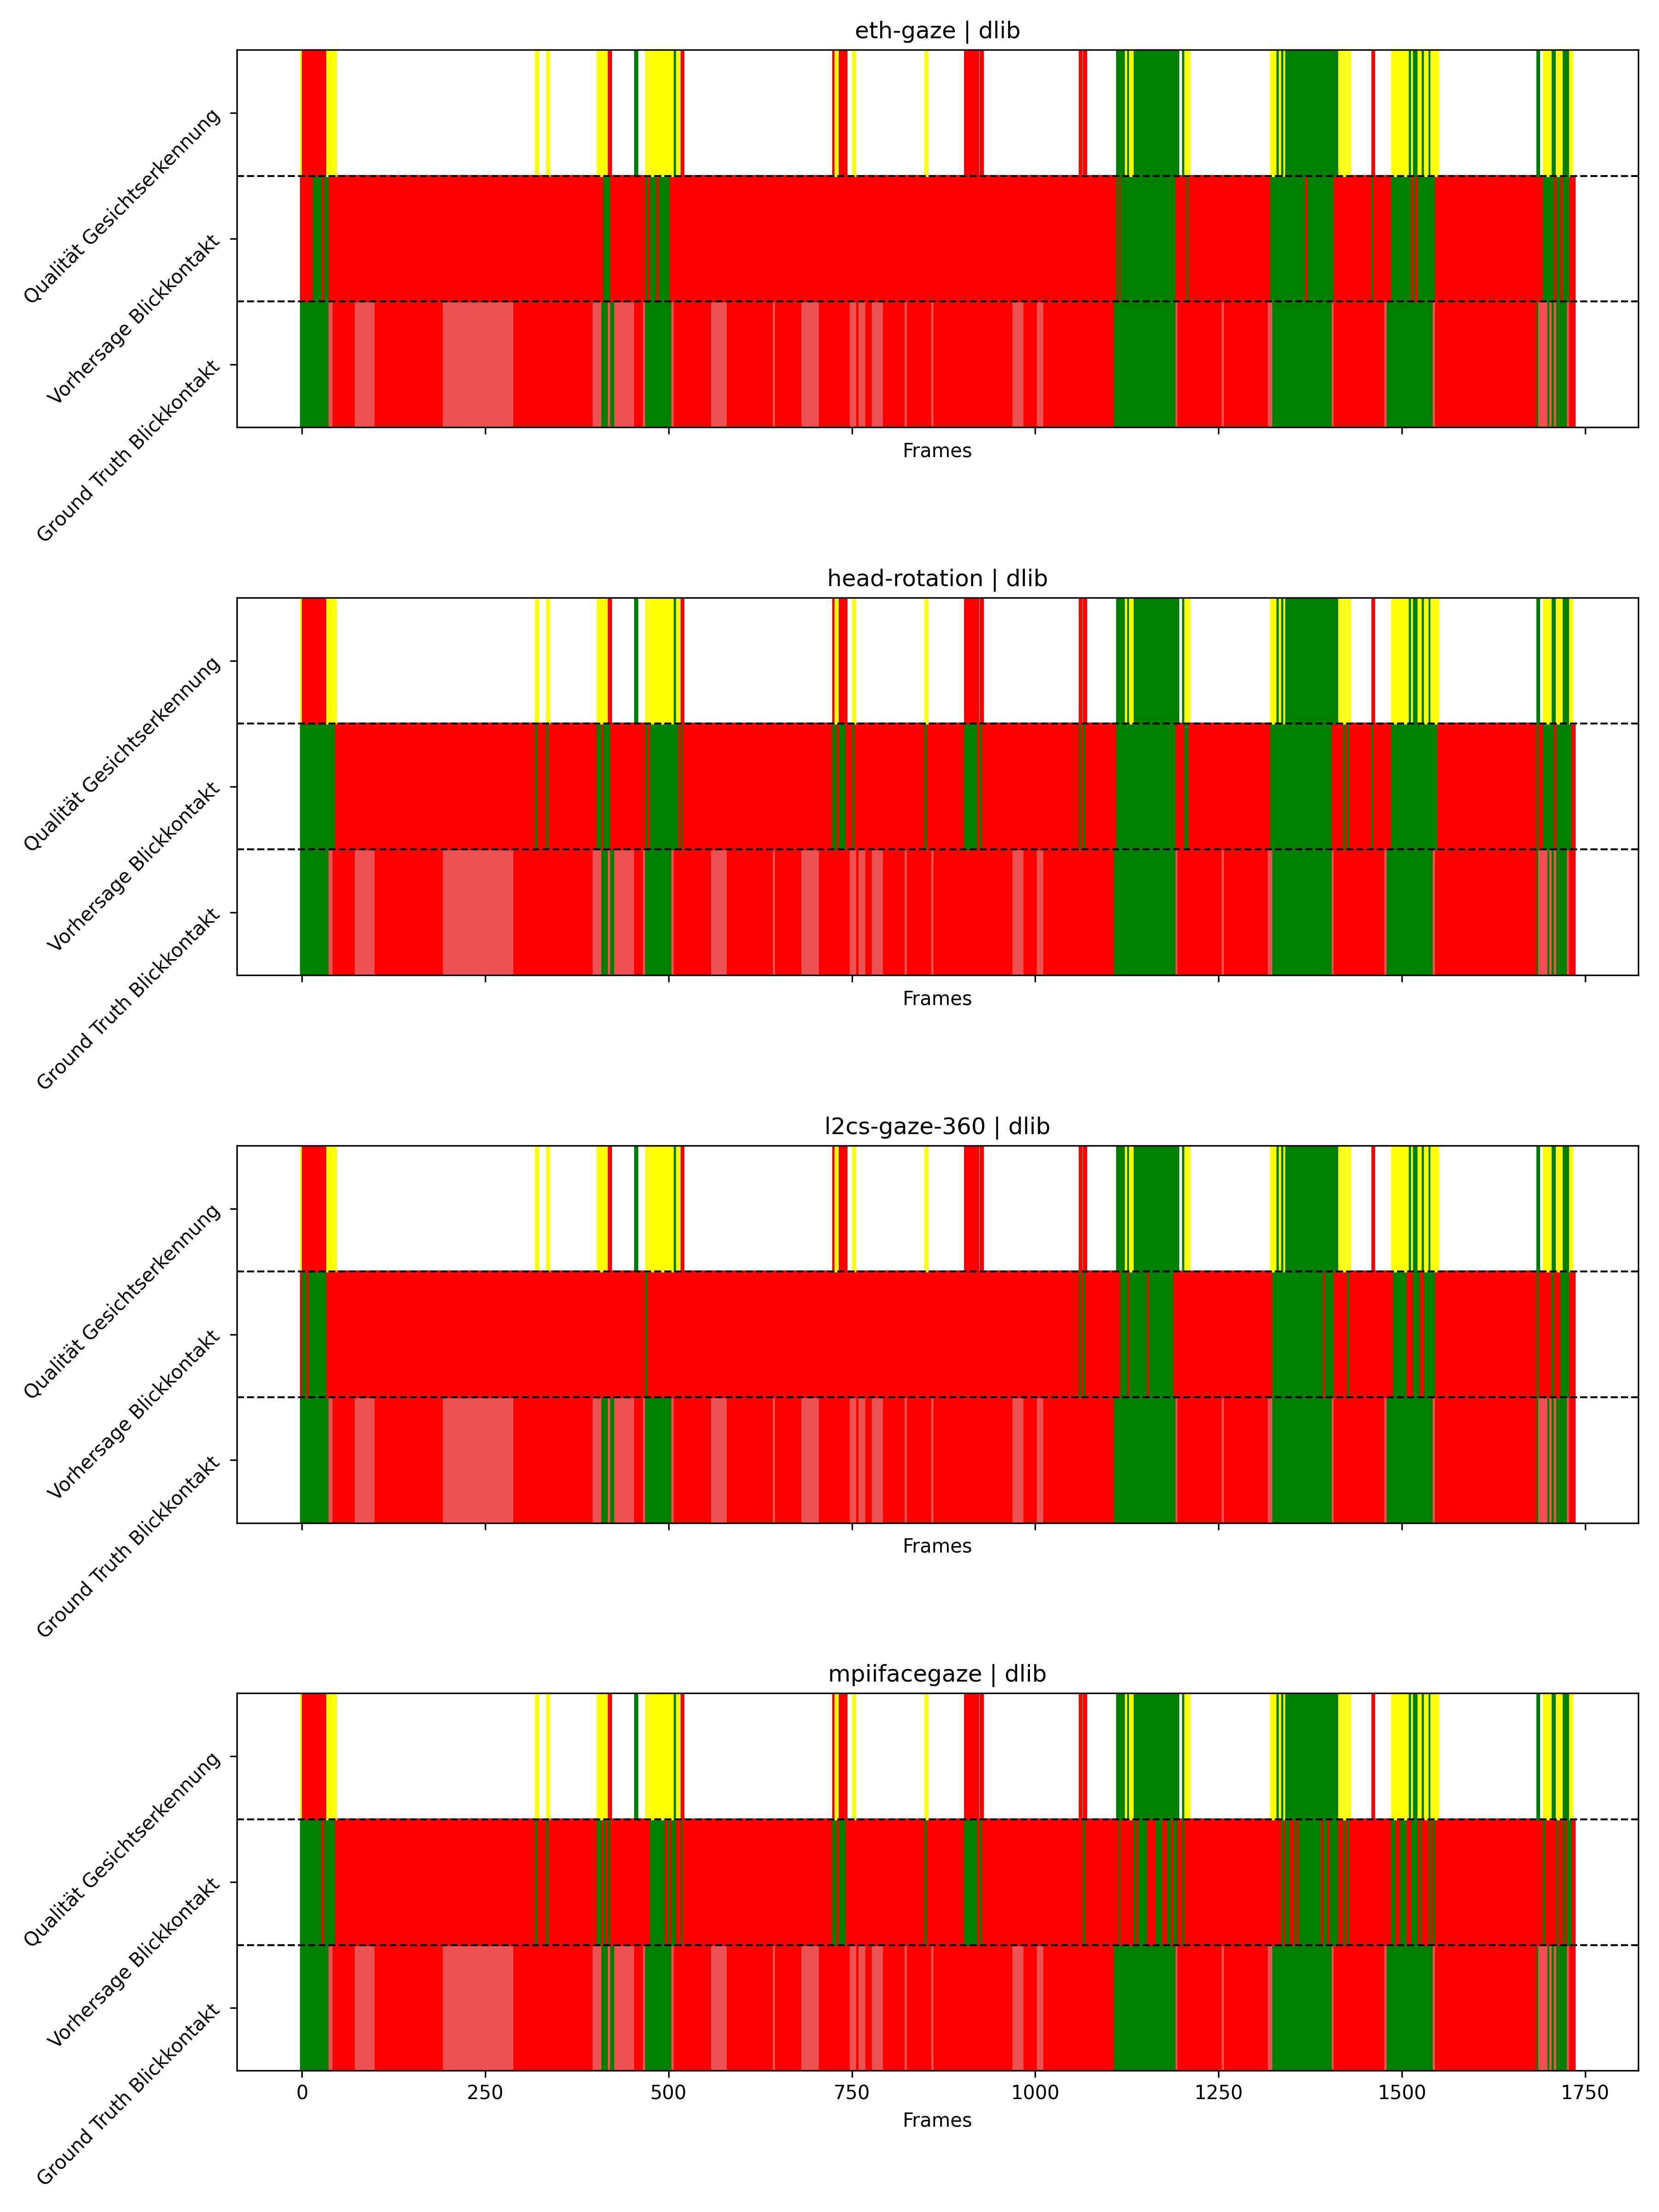
\includegraphics[width=1\linewidth]{appendix/24-dlib-overview-gaze.jpg}
\caption{Überblick über die Ground Truth des Blickkontakts, die Vorhersage des Blickkontakts und die Qualität der Gesichtserkennung mit \dlib. Die Bedeutung der Farben ist in Abbildung \ref{fig:evaluation:gaze:mpiifacegaze} erklärt.  }
\end{figure}

\begin{figure}[H]
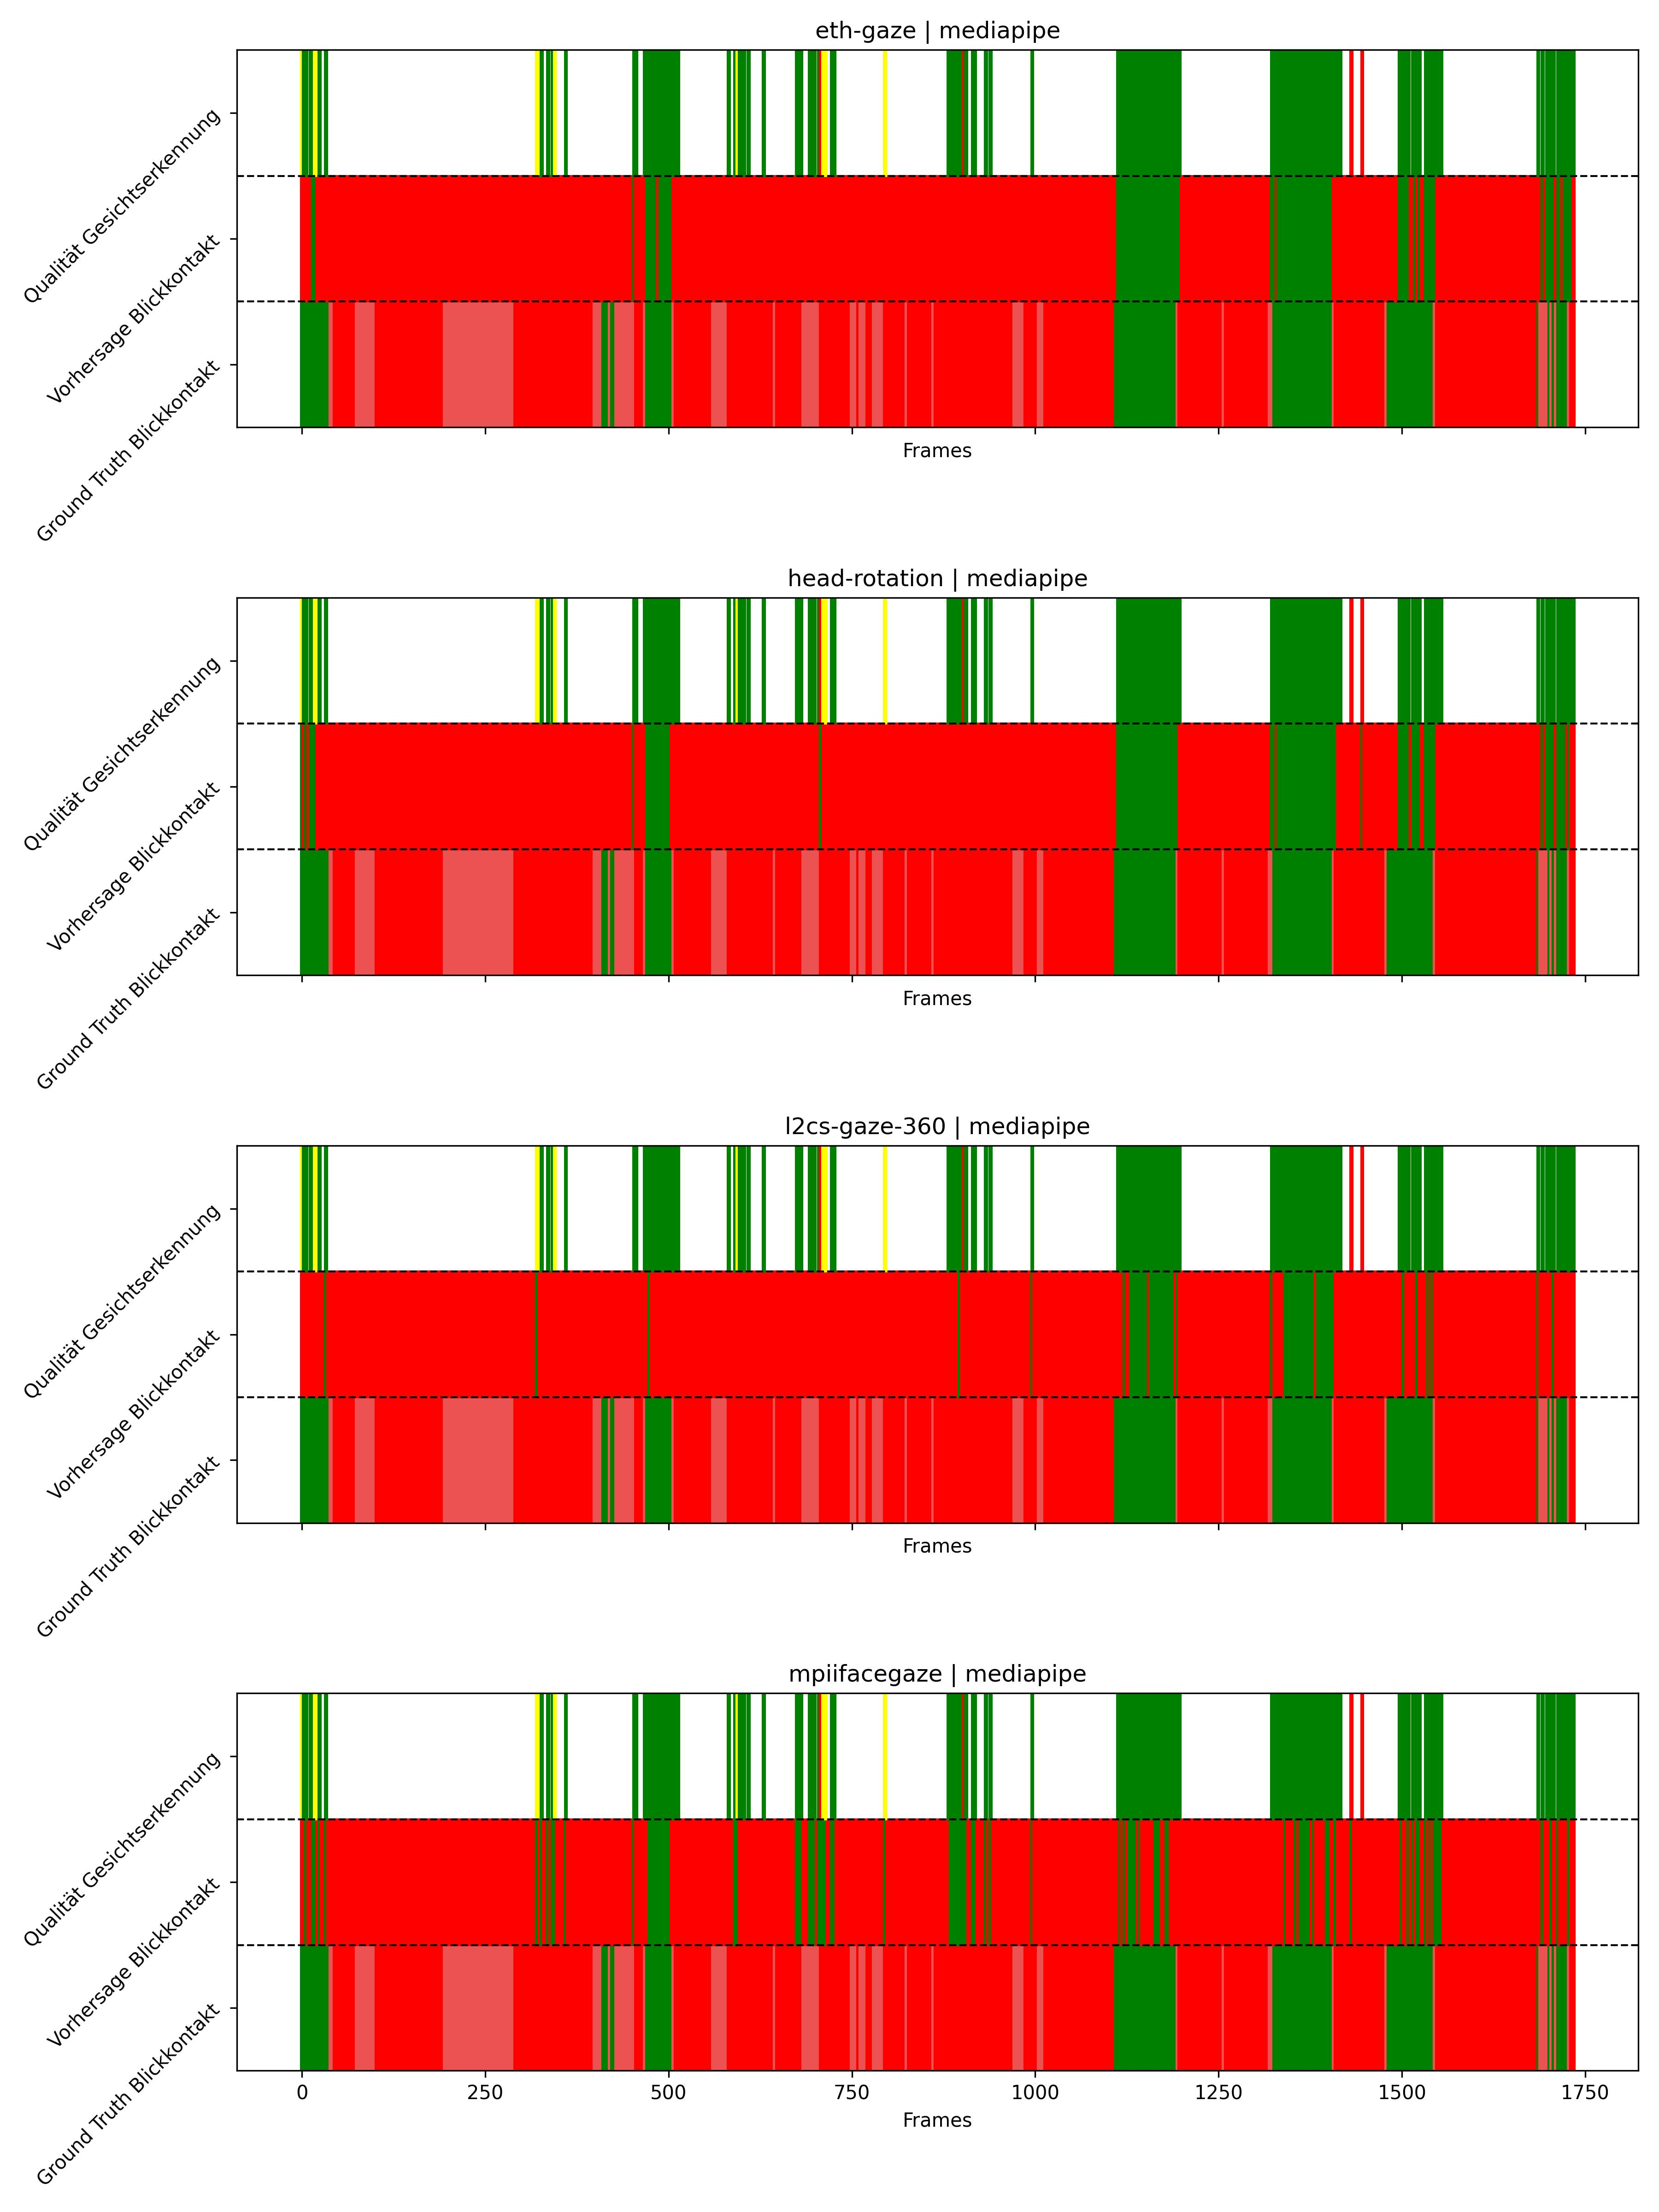
\includegraphics[width=1\linewidth]{appendix/24-mediapipe-overview-gaze.jpg}
\caption{Überblick über die Ground Truth des Blickkontakts, die Vorhersage des Blickkontakts und die Qualität der Gesichtserkennung mit \mediapipe. Die Bedeutung der Farben ist in Abbildung \ref{fig:evaluation:gaze:mpiifacegaze} erklärt.}
\end{figure}


  \end{appendices}

\end{document}
